%\pdfoutput=1
% Uncomment line above if submitting to arXiv and using pdflatex
% ============================================================================
% Purpose: Template for LHCb documents
% Authors: Tomasz Skwarnicki, Roger Forty, Ulrik Egede, Patrick Koppenburg
% Created on: 2010-09-24
% ============================================================================
\documentclass[12pt,a4paper]{article}
%%\documentclass[12pt,letter]{article}
% For two column text, add "twocolumn" as an option to the document
% class. Also uncomment the two "onecolumn" and "twocolumn" lines
% around the title page below.
% Variables that controls behaviour
\usepackage[page,toc,titletoc,title]{appendix}
\usepackage{ifthen} % for conditional statements
\newboolean{pdflatex}
\setboolean{pdflatex}{true} % False for eps figures 
\newboolean{articletitles}
\setboolean{articletitles}{true} % False removes titles in references
\newboolean{uprightparticles}
\setboolean{uprightparticles}{false} %True for upright particle symbols
%\newboolean{inbibliography}
%\setboolean{inbibliography}{false} %True once you enter the bibliography
% Define titles and authors here. It will then be used both in metadata and in
% what is printed on the front page.
\def\paperauthors{Xianglei Zhu, Youen Kang, Li Xu, Chenzhi Dong} % Leave as is for PAPER, CONF and FIGURE
\def\paperasciititle{Multiplicity Dependence of ratio of production of psi(2S) over J/psi in pp collision at center of mass energy 13 TeV} % Set ASCII title here !! MAKE sure it's only ASCII characters !! 
\def\papertitle{Multiplicity Dependence of $\sigma_{\psitwos}/\sigma_{\jpsi}$ in $pp$ collision at $\sqrt{s}=13$ TeV} % Latex formatted title
\def\paperkeywords{{High Energy Physics}, {LHCb}} % Comma separated list
%\def\papercopyright{CERN on behalf of the LHCb collaboration}
\def\papercopyright{\the\year\ CERN for the benefit of the LHCb collaboration} % new since 9/Apr/2018
\def\paperlicence{CC BY 4.0 licence}
\def\paperlicenceurl{https://creativecommons.org/licenses/by/4.0/}
%%%%%%%%%%%%%%%%%%%%%%%%%%%%%%%%%%%%%%%%%%%%%%%%%%%%%%%%%%%%%%%%%%%%%%
%                                                                    %
% !!!!!!!!!!!!!!!!!!! DO NOT EDIT THIS FILE !!!!!!!!!!!!!!!!!!!!!!!! %
%                                                                    %
% THE EB MAY OVERWRITE IT TO REFLECT LATEST CHANGES IN THE TEMPLATE  %
%                                                                    %
% You may define your own macros and packages in main.tex or add     %
% additional local files                                             %
%%%%%%%%%%%%%%%%%%%%%%%%%%%%%%%%%%%%%%%%%%%%%%%%%%%%%%%%%%%%%%%%%%%%%%
% THis file contains all the default packages and modifications for
% LHCb formatting

%% %%%%%%%%%%%%%%%%%%
%%  Page formatting
%% %%%%%%%%%%%%%%%%%%
%%\usepackage[margin=1in]{geometry}
\usepackage[top=1in, bottom=1.25in, left=1in, right=1in]{geometry}

% fallback for manual settings... uncomment if the geometry package is not available
%
%\voffset=-11mm
%\textheight=220mm
%\textwidth=160mm
%\oddsidemargin=0mm
%\evensidemargin=0mm

\columnsep=5mm
\addtolength{\belowcaptionskip}{0.5em}

\renewcommand{\textfraction}{0.01}
\renewcommand{\floatpagefraction}{0.8} % changed from 0.99
\renewcommand{\topfraction}{0.9}
\renewcommand{\bottomfraction}{0.9}

% Allow the page size to vary a bit ...
\raggedbottom
% To avoid Latex to be too fussy with line breaking ...
\sloppy

%% %%%%%%%%%%%%%%%%%%%%%%%
%% Packages to be used
%% %%%%%%%%%%%%%%%%%%%%%%% 
\usepackage{microtype}
\usepackage{lineno}  % for line numbering during review
\usepackage{xspace} % To avoid problems with missing or double spaces after
                    % predefined symbold
\usepackage{caption} %these three command get the figure and table captions automatically small
\renewcommand{\captionfont}{\small}
\renewcommand{\captionlabelfont}{\small}

%% Graphics
\usepackage{graphicx}  % to include figures (can also use other packages)
\usepackage{color}
\usepackage{colortbl}
\graphicspath{{./figs/}} % Make Latex search fig subdir for figures
% \DeclareGraphicsExtensions{.pdf,.PDF,.png,.PNG}   % not needed

%% Math
\usepackage{amsmath} % Adds a large collection of math symbols
\usepackage{amssymb}
\usepackage{amsfonts}
\usepackage{upgreek} % Adds in support for greek letters in roman typeset

%% fix to allow peaceful coexistence of line numbering and
%% mathematical objects
%% http://www.latex-community.org/forum/viewtopic.php?f=5&t=163
%%
\newcommand*\patchAmsMathEnvironmentForLineno[1]{%
\expandafter\let\csname old#1\expandafter\endcsname\csname #1\endcsname
\expandafter\let\csname oldend#1\expandafter\endcsname\csname
end#1\endcsname
 \renewenvironment{#1}%
   {\linenomath\csname old#1\endcsname}%
   {\csname oldend#1\endcsname\endlinenomath}%
}
\newcommand*\patchBothAmsMathEnvironmentsForLineno[1]{%
  \patchAmsMathEnvironmentForLineno{#1}%
  \patchAmsMathEnvironmentForLineno{#1*}%
}
\AtBeginDocument{%
\patchBothAmsMathEnvironmentsForLineno{equation}%
\patchBothAmsMathEnvironmentsForLineno{align}%
\patchBothAmsMathEnvironmentsForLineno{flalign}%
\patchBothAmsMathEnvironmentsForLineno{alignat}%
\patchBothAmsMathEnvironmentsForLineno{gather}%
\patchBothAmsMathEnvironmentsForLineno{multline}%
\patchBothAmsMathEnvironmentsForLineno{eqnarray}%
}

% Get hyperlinks to captions and in references.
% These do not work with revtex. Use "hypertext" as class option instead.

\usepackage{hyperxmp}

\usepackage[pdftex,
            pdfauthor={\paperauthors},
            pdftitle={\paperasciititle},
            pdfkeywords={\paperkeywords},
            pdfcopyright={Copyright (C) \papercopyright},
            pdflicenseurl={\paperlicenceurl}]{hyperref}
% if you have a mysterious compilation error at this line, check there are only ascii characters in \paperasciititle (main.tex)

% overleaf comments
\usepackage[colorinlistoftodos,textsize=scriptsize]{todonotes}

% get footnotes below floats
\usepackage[bottom,flushmargin,hang,multiple]{footmisc}

\usepackage[all]{hypcap} % Internal hyperlinks to floats.

%%%%%%%%%%%%%%%%%%%%%%%%%%%%%%%%%%%%%%%%%%%%%%%%%%%%%%%%%%%%%%%%%%%%%%%%
%%%                                                                    %
%%% !!!!!!!!!!!!!!!!!!! DO NOT EDIT THIS FILE !!!!!!!!!!!!!!!!!!!!!!!! %
%%%                                                                    %
%%% THE EB MAY OVERWRITE IT TO REFLECT LATEST CHANGES IN THE TEMPLATE  %
%%%                                                                    %
%%% You may define your own macros and packages in main.tex or add     %
%%% additional local files                                             %
%%%%%%%%%%%%%%%%%%%%%%%%%%%%%%%%%%%%%%%%%%%%%%%%%%%%%%%%%%%%%%%%%%%%%%%%
%%% ======================================================================
%%% Purpose: Standard LHCb aliases
%%% Author: Originally Ulrik Egede, adapted by Tomasz Skwarnicki for templates,
%%% rewritten by Chris Parkes
%%% Maintainer : Ulrik Egede (2010 - 2012)
%%% Maintainer : Rolf Oldeman (2012 - 2014)
%%% Maintainer : Patrick Koppenburg (2018--2020)
%%% =======================================================================
%%% To use this file outside the normal LHCb document environment, the
%%% following should be added in a preamble (before \begin{document}
%%%
%%%\usepackage{ifthen} 
%%%\newboolean{uprightparticles}
%%%\setboolean{uprightparticles}{false} %Set true for upright particle symbols
\usepackage{xspace} 
\usepackage{upgreek}


%%%%%%%%%%%%%%%%%%%%%%%%%%%%%%%%%%%%%%%%%%%%%%%%%%%%%%%%%%%%
%%%
%%% The following is to ensure that the template automatically can process
%%% this file.
%%%
%%% Add comments with at least three %%% preceding.
%%% Add new sections with one % preceding
%%% Add new subsections with two %% preceding
%%%
%%% For upper greek letters, Xires and Xiresbar will be the particles without the charge
%%% States with charge are called Xiz and Xim  
%%%
%%%%%%%%%%%%%%%%%%%%%%%%%%%%%%%%%%%%%%%%%%%%%%%%%%%%%%%%%%%%

%%%%%%%%%%%%%
% Experiments
%%%%%%%%%%%%%
\def\lhcb   {\mbox{LHCb}\xspace}
\def\atlas  {\mbox{ATLAS}\xspace}
\def\cms    {\mbox{CMS}\xspace}
\def\alice  {\mbox{ALICE}\xspace}
\def\babar  {\mbox{BaBar}\xspace}
\def\belle  {\mbox{Belle}\xspace}
\def\belletwo {\mbox{Belle~II}\xspace}
\def\besiii {\mbox{BESIII}\xspace}
\def\cleo   {\mbox{CLEO}\xspace}
\def\cdf    {\mbox{CDF}\xspace}
\def\dzero  {\mbox{D0}\xspace}
\def\aleph  {\mbox{ALEPH}\xspace}
\def\delphi {\mbox{DELPHI}\xspace}
\def\opal   {\mbox{OPAL}\xspace}
\def\lthree {\mbox{L3}\xspace}
\def\sld    {\mbox{SLD}\xspace}
%%%\def\argus  {\mbox{ARGUS}\xspace}
%%%\def\uaone  {\mbox{UA1}\xspace}
%%%\def\uatwo  {\mbox{UA2}\xspace}
%%%\def\ux85 {\mbox{UX85}\xspace}
\def\cern {\mbox{CERN}\xspace}
\def\lhc    {\mbox{LHC}\xspace}
\def\lep    {\mbox{LEP}\xspace}
\def\tevatron {Tevatron\xspace}
\def\bfactories {\mbox{\B Factories}\xspace}
\def\bfactory   {\mbox{\B Factory}\xspace}
\def\upgradeone {\mbox{Upgrade~I}\xspace}
\def\upgradetwo {\mbox{Upgrade~II}\xspace}

%% LHCb sub-detectors and sub-systems

%%%\def\pu     {PU\xspace}
\def\velo   {VELO\xspace}
\def\rich   {RICH\xspace}
\def\richone {RICH1\xspace}
\def\richtwo {RICH2\xspace}
\def\ttracker {TT\xspace}
\def\intr   {IT\xspace}
\def\st     {ST\xspace}
\def\ot     {OT\xspace}
\def\herschel {\mbox{\textsc{HeRSCheL}}\xspace}
%%%\def\Tone   {T1\xspace}
%%%\def\Ttwo   {T2\xspace}
%%%\def\Tthree {T3\xspace}
%%%\def\Mone   {M1\xspace}
%%%\def\Mtwo   {M2\xspace}
%%%\def\Mthree {M3\xspace}
%%%\def\Mfour  {M4\xspace}
%%%\def\Mfive  {M5\xspace}
\def\spd    {SPD\xspace}
\def\presh  {PS\xspace}
\def\ecal   {ECAL\xspace}
\def\hcal   {HCAL\xspace}
%%%\def\bcm    {BCM\xspace}
\def\MagUp {\mbox{\em Mag\kern -0.05em Up}\xspace}
\def\MagDown {\mbox{\em MagDown}\xspace}

\def\ode    {ODE\xspace}
\def\daq    {DAQ\xspace}
\def\tfc    {TFC\xspace}
\def\ecs    {ECS\xspace}
\def\lone   {L0\xspace}
\def\hlt    {HLT\xspace}
\def\hltone {HLT1\xspace}
\def\hlttwo {HLT2\xspace}

%%% Upright (not slanted) Particles

\ifthenelse{\boolean{uprightparticles}}%
{\def\Palpha      {\ensuremath{\upalpha}\xspace}
 \def\Pbeta       {\ensuremath{\upbeta}\xspace}
 \def\Pgamma      {\ensuremath{\upgamma}\xspace}                 
 \def\Pdelta      {\ensuremath{\updelta}\xspace}                 
 \def\Pepsilon    {\ensuremath{\upepsilon}\xspace}                 
 \def\Pvarepsilon {\ensuremath{\upvarepsilon}\xspace}                 
 \def\Pzeta       {\ensuremath{\upzeta}\xspace}                 
 \def\Peta        {\ensuremath{\upeta}\xspace}
 \def\Ptheta      {\ensuremath{\uptheta}\xspace}                 
 \def\Pvartheta   {\ensuremath{\upvartheta}\xspace}                 
 \def\Piota       {\ensuremath{\upiota}\xspace}                 
 \def\Pkappa      {\ensuremath{\upkappa}\xspace}                 
 \def\Plambda     {\ensuremath{\uplambda}\xspace}                 
 \def\Pmu         {\ensuremath{\upmu}\xspace}                 
 \def\Pnu         {\ensuremath{\upnu}\xspace}                 
 \def\Pxi         {\ensuremath{\upxi}\xspace}                 
 \def\Ppi         {\ensuremath{\uppi}\xspace}                 
 \def\Pvarpi      {\ensuremath{\upvarpi}\xspace}                 
 \def\Prho        {\ensuremath{\uprho}\xspace}                 
 \def\Pvarrho     {\ensuremath{\upvarrho}\xspace}                 
 \def\Ptau        {\ensuremath{\uptau}\xspace}                 
 \def\Pupsilon    {\ensuremath{\upupsilon}\xspace}                 
 \def\Pphi        {\ensuremath{\upphi}\xspace}                 
 \def\Pvarphi     {\ensuremath{\upvarphi}\xspace}                 
 \def\Pchi        {\ensuremath{\upchi}\xspace}                 
 \def\Ppsi        {\ensuremath{\uppsi}\xspace}                 
 \def\Pomega      {\ensuremath{\upomega}\xspace}                 

 \def\PDelta      {\ensuremath{\Delta}\xspace}                 
 \def\PXi         {\ensuremath{\Xi}\xspace}                 
 \def\PLambda     {\ensuremath{\Lambda}\xspace}                 
 \def\PSigma      {\ensuremath{\Sigma}\xspace}                 
 \def\POmega      {\ensuremath{\Omega}\xspace}                 
 \def\PUpsilon    {\ensuremath{\Upsilon}\xspace}
 \let\oldPi\Pi
 \def\PPi         {\ensuremath{\oldPi}\xspace}                 
               

 \def\PA      {\ensuremath{\mathrm{A}}\xspace}                 
 \def\PB      {\ensuremath{\mathrm{B}}\xspace}                 
 \def\PC      {\ensuremath{\mathrm{C}}\xspace}                 
 \def\PD      {\ensuremath{\mathrm{D}}\xspace}                 
 \def\PE      {\ensuremath{\mathrm{E}}\xspace}                 
 \def\PF      {\ensuremath{\mathrm{F}}\xspace}                 
 \def\PG      {\ensuremath{\mathrm{G}}\xspace}                 
 \def\PH      {\ensuremath{\mathrm{H}}\xspace}                 
 \def\PI      {\ensuremath{\mathrm{I}}\xspace}                 
 \def\PJ      {\ensuremath{\mathrm{J}}\xspace}                 
 \def\PK      {\ensuremath{\mathrm{K}}\xspace}                 
 \def\PL      {\ensuremath{\mathrm{L}}\xspace}                 
 \def\PM      {\ensuremath{\mathrm{M}}\xspace}                 
 \def\PN      {\ensuremath{\mathrm{N}}\xspace}                 
 \def\PO      {\ensuremath{\mathrm{O}}\xspace}                 
 \def\PP      {\ensuremath{\mathrm{P}}\xspace}                 
 \def\PQ      {\ensuremath{\mathrm{Q}}\xspace}                 
 \def\PR      {\ensuremath{\mathrm{R}}\xspace}                 
 \def\PS      {\ensuremath{\mathrm{S}}\xspace}                 
 \def\PT      {\ensuremath{\mathrm{T}}\xspace}                 
 \def\PU      {\ensuremath{\mathrm{U}}\xspace}                 
 \def\PV      {\ensuremath{\mathrm{V}}\xspace}                 
 \def\PW      {\ensuremath{\mathrm{W}}\xspace}                 
 \def\PX      {\ensuremath{\mathrm{X}}\xspace}                 
 \def\PY      {\ensuremath{\mathrm{Y}}\xspace}                 
 \def\PZ      {\ensuremath{\mathrm{Z}}\xspace}                 
 \def\Pa      {\ensuremath{\mathrm{a}}\xspace}                 
 \def\Pb      {\ensuremath{\mathrm{b}}\xspace}                 
 \def\Pc      {\ensuremath{\mathrm{c}}\xspace}                 
 \def\Pd      {\ensuremath{\mathrm{d}}\xspace}                 
 \def\Pe      {\ensuremath{\mathrm{e}}\xspace}                 
 \def\Pf      {\ensuremath{\mathrm{f}}\xspace}                 
 \def\Pg      {\ensuremath{\mathrm{g}}\xspace}                 
 \def\Ph      {\ensuremath{\mathrm{h}}\xspace}                 
 \def\Pi      {\ensuremath{\mathrm{i}}\xspace}                 
 \def\Pj      {\ensuremath{\mathrm{j}}\xspace}                 
 \def\Pk      {\ensuremath{\mathrm{k}}\xspace}                 
 \def\Pl      {\ensuremath{\mathrm{l}}\xspace}                 
 \def\Pm      {\ensuremath{\mathrm{m}}\xspace}                 
 \def\Pn      {\ensuremath{\mathrm{n}}\xspace}                 
 \def\Po      {\ensuremath{\mathrm{o}}\xspace}                 
 \def\Pp      {\ensuremath{\mathrm{p}}\xspace}                 
 \def\Pq      {\ensuremath{\mathrm{q}}\xspace}                 
 \def\Pr      {\ensuremath{\mathrm{r}}\xspace}                 
 \def\Ps      {\ensuremath{\mathrm{s}}\xspace}                 
 \def\Pt      {\ensuremath{\mathrm{t}}\xspace}                 
 \def\Pu      {\ensuremath{\mathrm{u}}\xspace}                 
 \def\Pv      {\ensuremath{\mathrm{v}}\xspace}                 
 \def\Pw      {\ensuremath{\mathrm{w}}\xspace}                 
 \def\Px      {\ensuremath{\mathrm{x}}\xspace}                 
 \def\Py      {\ensuremath{\mathrm{y}}\xspace}                 
 \def\Pz      {\ensuremath{\mathrm{z}}\xspace}                 
 \def\thebaroffset{0.0em}
}
{\def\Palpha      {\ensuremath{\alpha}\xspace}
 \def\Pbeta       {\ensuremath{\beta}\xspace}
 \def\Pgamma      {\ensuremath{\gamma}\xspace}                 
 \def\Pdelta      {\ensuremath{\delta}\xspace}                 
 \def\Pepsilon    {\ensuremath{\epsilon}\xspace}                 
 \def\Pvarepsilon {\ensuremath{\varepsilon}\xspace}                 
 \def\Pzeta       {\ensuremath{\zeta}\xspace}                 
 \def\Peta        {\ensuremath{\eta}\xspace}                 
 \def\Ptheta      {\ensuremath{\theta}\xspace}                 
 \def\Pvartheta   {\ensuremath{\vartheta}\xspace}                 
 \def\Piota       {\ensuremath{\iota}\xspace}                 
 \def\Pkappa      {\ensuremath{\kappa}\xspace}                 
 \def\Plambda     {\ensuremath{\lambda}\xspace}                 
 \def\Pmu         {\ensuremath{\mu}\xspace}                 
 \def\Pnu         {\ensuremath{\nu}\xspace}                 
 \def\Pxi         {\ensuremath{\xi}\xspace}                 
 \def\Ppi         {\ensuremath{\pi}\xspace}                 
 \def\Pvarpi      {\ensuremath{\varpi}\xspace}                 
 \def\Prho        {\ensuremath{\rho}\xspace}                 
 \def\Pvarrho     {\ensuremath{\varrho}\xspace}                 
 \def\Ptau        {\ensuremath{\tau}\xspace}                 
 \def\Pupsilon    {\ensuremath{\upsilon}\xspace}                 
 \def\Pphi        {\ensuremath{\phi}\xspace}                 
 \def\Pvarphi     {\ensuremath{\varphi}\xspace}                 
 \def\Pchi        {\ensuremath{\chi}\xspace}                 
 \def\Ppsi        {\ensuremath{\psi}\xspace}                 
 \def\Pomega      {\ensuremath{\omega}\xspace}                 
 \mathchardef\PDelta="7101
 \mathchardef\PXi="7104
 \mathchardef\PLambda="7103
 \mathchardef\PSigma="7106
 \mathchardef\POmega="710A
 \mathchardef\PUpsilon="7107
 \mathchardef\PPi="7105
 \def\PA      {\ensuremath{A}\xspace}                 
 \def\PB      {\ensuremath{B}\xspace}                 
 \def\PC      {\ensuremath{C}\xspace}                 
 \def\PD      {\ensuremath{D}\xspace}                 
 \def\PE      {\ensuremath{E}\xspace}                 
 \def\PF      {\ensuremath{F}\xspace}                 
 \def\PG      {\ensuremath{G}\xspace}                 
 \def\PH      {\ensuremath{H}\xspace}                 
 \def\PI      {\ensuremath{I}\xspace}                 
 \def\PJ      {\ensuremath{J}\xspace}                 
 \def\PK      {\ensuremath{K}\xspace}                 
 \def\PL      {\ensuremath{L}\xspace}                 
 \def\PM      {\ensuremath{M}\xspace}                 
 \def\PN      {\ensuremath{N}\xspace}                 
 \def\PO      {\ensuremath{O}\xspace}                 
 \def\PP      {\ensuremath{P}\xspace}                 
 \def\PQ      {\ensuremath{Q}\xspace}                 
 \def\PR      {\ensuremath{R}\xspace}                 
 \def\PS      {\ensuremath{S}\xspace}                 
 \def\PT      {\ensuremath{T}\xspace}                 
 \def\PU      {\ensuremath{U}\xspace}                 
 \def\PV      {\ensuremath{V}\xspace}                 
 \def\PW      {\ensuremath{W}\xspace}                 
 \def\PX      {\ensuremath{X}\xspace}                 
 \def\PY      {\ensuremath{Y}\xspace}                 
 \def\PZ      {\ensuremath{Z}\xspace}                 
 \def\Pa      {\ensuremath{a}\xspace}                 
 \def\Pb      {\ensuremath{b}\xspace}                 
 \def\Pc      {\ensuremath{c}\xspace}                 
 \def\Pd      {\ensuremath{d}\xspace}                 
 \def\Pe      {\ensuremath{e}\xspace}                 
 \def\Pf      {\ensuremath{f}\xspace}                 
 \def\Pg      {\ensuremath{g}\xspace}                 
 \def\Ph      {\ensuremath{h}\xspace}                 
 \def\Pi      {\ensuremath{i}\xspace}                 
 \def\Pj      {\ensuremath{j}\xspace}                 
 \def\Pk      {\ensuremath{k}\xspace}                 
 \def\Pl      {\ensuremath{l}\xspace}                 
 \def\Pm      {\ensuremath{m}\xspace}                 
 \def\Pn      {\ensuremath{n}\xspace}                 
 \def\Po      {\ensuremath{o}\xspace}                 
 \def\Pp      {\ensuremath{p}\xspace}                 
 \def\Pq      {\ensuremath{q}\xspace}                 
 \def\Pr      {\ensuremath{r}\xspace}                 
 \def\Ps      {\ensuremath{s}\xspace}                 
 \def\Pt      {\ensuremath{t}\xspace}                 
 \def\Pu      {\ensuremath{u}\xspace}                 
 \def\Pv      {\ensuremath{v}\xspace}                 
 \def\Pw      {\ensuremath{w}\xspace}                 
 \def\Px      {\ensuremath{x}\xspace}                 
 \def\Py      {\ensuremath{y}\xspace}                 
 \def\Pz      {\ensuremath{z}\xspace}
 \def\thebaroffset{0.18em}
}
\newcommand{\offsetoverline}[2][\thebaroffset]{\kern #1\overline{\kern -#1 #2}}%

%%%%%%%%%%%%%%%%%%%%%%%%%%%%%%%%%%%%%%%%%%%%%%%
% Particles
\makeatletter
\ifcase \@ptsize \relax% 10pt
  \newcommand{\miniscule}{\@setfontsize\miniscule{4}{5}}% \tiny: 5/6
\or% 11pt
  \newcommand{\miniscule}{\@setfontsize\miniscule{5}{6}}% \tiny: 6/7
\or% 12pt
  \newcommand{\miniscule}{\@setfontsize\miniscule{5}{6}}% \tiny: 6/7
\fi
\makeatother


\DeclareRobustCommand{\optbar}[1]{\shortstack{{\miniscule (\rule[.5ex]{1.25em}{.18mm})}
  \\ [-.7ex] $#1$}}


%% Leptons

\let\emi\en
\def\electron   {{\ensuremath{\Pe}}\xspace}
\def\en         {{\ensuremath{\Pe^-}}\xspace}   % electron negative (\em is taken)
\def\ep         {{\ensuremath{\Pe^+}}\xspace}
\def\epm        {{\ensuremath{\Pe^\pm}}\xspace} 
\def\emp        {{\ensuremath{\Pe^\mp}}\xspace} 
\def\epem       {{\ensuremath{\Pe^+\Pe^-}}\xspace}
%%%\def\ee         {\ensuremath{\Pe^-\Pe^-}\xspace}

\def\muon       {{\ensuremath{\Pmu}}\xspace}
\def\mup        {{\ensuremath{\Pmu^+}}\xspace}
\def\mun        {{\ensuremath{\Pmu^-}}\xspace} % muon negative (\mum is taken)
\def\mupm       {{\ensuremath{\Pmu^\pm}}\xspace} 
\def\mump       {{\ensuremath{\Pmu^\mp}}\xspace} 
\def\mumu       {{\ensuremath{\Pmu^+\Pmu^-}}\xspace}

\def\tauon      {{\ensuremath{\Ptau}}\xspace}
\def\taup       {{\ensuremath{\Ptau^+}}\xspace}
\def\taum       {{\ensuremath{\Ptau^-}}\xspace}
\def\taupm      {{\ensuremath{\Ptau^\pm}}\xspace}
\def\taump      {{\ensuremath{\Ptau^\mp}}\xspace}
\def\tautau     {{\ensuremath{\Ptau^+\Ptau^-}}\xspace}

\def\lepton     {{\ensuremath{\ell}}\xspace}
\def\ellm       {{\ensuremath{\ell^-}}\xspace}
\def\ellp       {{\ensuremath{\ell^+}}\xspace}
\def\ellpm      {{\ensuremath{\ell^\pm}}\xspace}
\def\ellmp      {{\ensuremath{\ell^\mp}}\xspace}
\def\ellell     {\ensuremath{\ell^+ \ell^-}\xspace}

\def\neu        {{\ensuremath{\Pnu}}\xspace}
\def\neub       {{\ensuremath{\overline{\Pnu}}}\xspace}
%%%\def\nuenueb    {\ensuremath{\neu\neub}\xspace}
\def\neue       {{\ensuremath{\neu_e}}\xspace}
\def\neueb      {{\ensuremath{\neub_e}}\xspace}
%%%\def\neueneueb  {\ensuremath{\neue\neueb}\xspace}
\def\neum       {{\ensuremath{\neu_\mu}}\xspace}
\def\neumb      {{\ensuremath{\neub_\mu}}\xspace}
%%%\def\neumneumb  {\ensuremath{\neum\neumb}\xspace}
\def\neut       {{\ensuremath{\neu_\tau}}\xspace}
\def\neutb      {{\ensuremath{\neub_\tau}}\xspace}
%%%\def\neutneutb  {\ensuremath{\neut\neutb}\xspace}
\def\neul       {{\ensuremath{\neu_\ell}}\xspace}
\def\neulb      {{\ensuremath{\neub_\ell}}\xspace}
%%%\def\neulneulb  {\ensuremath{\neul\neulb}\xspace}

%% Gauge bosons and scalars

\def\g      {{\ensuremath{\Pgamma}}\xspace}
\def\H      {{\ensuremath{\PH^0}}\xspace}
\def\Hp     {{\ensuremath{\PH^+}}\xspace}
\def\Hm     {{\ensuremath{\PH^-}}\xspace}
\def\Hpm    {{\ensuremath{\PH^\pm}}\xspace}
\def\W      {{\ensuremath{\PW}}\xspace}
\def\Wp     {{\ensuremath{\PW^+}}\xspace}
\def\Wm     {{\ensuremath{\PW^-}}\xspace}
\def\Wpm    {{\ensuremath{\PW^\pm}}\xspace}
\def\Z      {{\ensuremath{\PZ}}\xspace}

%% Quarks

\def\quark     {{\ensuremath{\Pq}}\xspace}
\def\quarkbar  {{\ensuremath{\overline \quark}}\xspace}
\def\qqbar     {{\ensuremath{\quark\quarkbar}}\xspace}
\def\uquark    {{\ensuremath{\Pu}}\xspace}
\def\uquarkbar {{\ensuremath{\overline \uquark}}\xspace}
\def\uubar     {{\ensuremath{\uquark\uquarkbar}}\xspace}
\def\dquark    {{\ensuremath{\Pd}}\xspace}
\def\dquarkbar {{\ensuremath{\overline \dquark}}\xspace}
\def\ddbar     {{\ensuremath{\dquark\dquarkbar}}\xspace}
\def\squark    {{\ensuremath{\Ps}}\xspace}
\def\squarkbar {{\ensuremath{\overline \squark}}\xspace}
\def\ssbar     {{\ensuremath{\squark\squarkbar}}\xspace}
\def\cquark    {{\ensuremath{\Pc}}\xspace}
\def\cquarkbar {{\ensuremath{\overline \cquark}}\xspace}
\def\ccbar     {{\ensuremath{\cquark\cquarkbar}}\xspace}
\def\bquark    {{\ensuremath{\Pb}}\xspace}
\def\bquarkbar {{\ensuremath{\overline \bquark}}\xspace}
\def\bbbar     {{\ensuremath{\bquark\bquarkbar}}\xspace}
\def\tquark    {{\ensuremath{\Pt}}\xspace}
\def\tquarkbar {{\ensuremath{\overline \tquark}}\xspace}
\def\ttbar     {{\ensuremath{\tquark\tquarkbar}}\xspace}

%% Light mesons

\def\hadron {{\ensuremath{\Ph}}\xspace}
\def\pion   {{\ensuremath{\Ppi}}\xspace}
\def\piz    {{\ensuremath{\pion^0}}\xspace}
\def\pip    {{\ensuremath{\pion^+}}\xspace}
\def\pim    {{\ensuremath{\pion^-}}\xspace}
\def\pipm   {{\ensuremath{\pion^\pm}}\xspace}
\def\pimp   {{\ensuremath{\pion^\mp}}\xspace}

\def\rhomeson {{\ensuremath{\Prho}}\xspace}
\def\rhoz     {{\ensuremath{\rhomeson^0}}\xspace}
\def\rhop     {{\ensuremath{\rhomeson^+}}\xspace}
\def\rhom     {{\ensuremath{\rhomeson^-}}\xspace}
\def\rhopm    {{\ensuremath{\rhomeson^\pm}}\xspace}
\def\rhomp    {{\ensuremath{\rhomeson^\mp}}\xspace}

\def\kaon    {{\ensuremath{\PK}}\xspace}
%%% do NOT use ensuremath here, and keep indent
\def\Kbar    {{\ensuremath{\offsetoverline{\PK}}}\xspace}
\def\Kb      {{\ensuremath{\Kbar}}\xspace}
\def\KorKbar {\kern \thebaroffset\optbar{\kern -\thebaroffset \PK}{}\xspace}
\def\Kz      {{\ensuremath{\kaon^0}}\xspace}
\def\Kzb     {{\ensuremath{\Kbar{}^0}}\xspace}
\def\Kp      {{\ensuremath{\kaon^+}}\xspace}
\def\Km      {{\ensuremath{\kaon^-}}\xspace}
\def\Kpm     {{\ensuremath{\kaon^\pm}}\xspace}
\def\Kmp     {{\ensuremath{\kaon^\mp}}\xspace}
\def\KS      {{\ensuremath{\kaon^0_{\mathrm{S}}}}\xspace}
\def\Vzero   {{\ensuremath{V^0}}\xspace}
\def\KL      {{\ensuremath{\kaon^0_{\mathrm{L}}}}\xspace}
\def\Kstarz  {{\ensuremath{\kaon^{*0}}}\xspace}
\def\Kstarzb {{\ensuremath{\Kbar{}^{*0}}}\xspace}
\def\Kstar   {{\ensuremath{\kaon^*}}\xspace}
\def\Kstarb  {{\ensuremath{\Kbar{}^*}}\xspace}
\def\Kstarp  {{\ensuremath{\kaon^{*+}}}\xspace}
\def\Kstarm  {{\ensuremath{\kaon^{*-}}}\xspace}
\def\Kstarpm {{\ensuremath{\kaon^{*\pm}}}\xspace}
\def\Kstarmp {{\ensuremath{\kaon^{*\mp}}}\xspace}
\def\KorKbarz {\ensuremath{\KorKbar^0}\xspace}

\newcommand{\etaz}{\ensuremath{\Peta}\xspace}
\newcommand{\etapr}{\ensuremath{\Peta^{\prime}}\xspace}
\newcommand{\phiz}{\ensuremath{\Pphi}\xspace}
\newcommand{\omegaz}{\ensuremath{\Pomega}\xspace}

%% Charmed mesons

%%% do NOT use ensuremath here (and keep indent)
\def\Dbar    {{\ensuremath{\offsetoverline{\PD}}}\xspace}
\def\D       {{\ensuremath{\PD}}\xspace}
\def\Db      {{\ensuremath{\Dbar}}\xspace}
\def\DorDbar {\kern \thebaroffset\optbar{\kern -\thebaroffset \PD}\xspace}
\def\Dz      {{\ensuremath{\D^0}}\xspace}
\def\Dzb     {{\ensuremath{\Dbar{}^0}}\xspace}
\def\Dp      {{\ensuremath{\D^+}}\xspace}
\def\Dm      {{\ensuremath{\D^-}}\xspace}
\def\Dpm     {{\ensuremath{\D^\pm}}\xspace}
\def\Dmp     {{\ensuremath{\D^\mp}}\xspace}
\def\DpDm    {\ensuremath{\Dp {\kern -0.16em \Dm}}\xspace}
\def\Dstar   {{\ensuremath{\D^*}}\xspace}
\def\Dstarb  {{\ensuremath{\Dbar{}^*}}\xspace}
\def\Dstarz  {{\ensuremath{\D^{*0}}}\xspace}
\def\Dstarzb {{\ensuremath{\Dbar{}^{*0}}}\xspace}
\def\theDstarz{{\ensuremath{\D^{*}(2007)^{0}}}\xspace}
\def\theDstarzb{{\ensuremath{\Dbar^{*}(2007)^{0}}}\xspace}
\def\Dstarp  {{\ensuremath{\D^{*+}}}\xspace}
\def\Dstarm  {{\ensuremath{\D^{*-}}}\xspace}
\def\Dstarpm {{\ensuremath{\D^{*\pm}}}\xspace}
\def\Dstarmp {{\ensuremath{\D^{*\mp}}}\xspace}
\def\theDstarp{{\ensuremath{\D^{*}(2010)^{+}}}\xspace}
\def\theDstarm{{\ensuremath{\D^{*}(2010)^{-}}}\xspace}
\def\theDstarpm{{\ensuremath{\D^{*}(2010)^{\pm}}}\xspace}
\def\theDstarmp{{\ensuremath{\D^{*}(2010)^{\mp}}}\xspace}
\def\Ds      {{\ensuremath{\D^+_\squark}}\xspace}
\def\Dsp     {{\ensuremath{\D^+_\squark}}\xspace}
\def\Dsm     {{\ensuremath{\D^-_\squark}}\xspace}
\def\Dspm    {{\ensuremath{\D^{\pm}_\squark}}\xspace}
\def\Dsmp    {{\ensuremath{\D^{\mp}_\squark}}\xspace}
\def\Dss     {{\ensuremath{\D^{*+}_\squark}}\xspace}
\def\Dssp    {{\ensuremath{\D^{*+}_\squark}}\xspace}
\def\Dssm    {{\ensuremath{\D^{*-}_\squark}}\xspace}
\def\Dsspm   {{\ensuremath{\D^{*\pm}_\squark}}\xspace}
\def\Dssmp   {{\ensuremath{\D^{*\mp}_\squark}}\xspace}
\def\DporDsp {{\ensuremath{\D_{(\squark)}^+}}\xspace}
\def\DmorDsm {{\ensuremath{\D{}_{(\squark)}^-}}\xspace}
\def\DpmorDspm {{\ensuremath{\D{}_{(\squark)}^\pm}}\xspace}

%% Beauty mesons
\def\B       {{\ensuremath{\PB}}\xspace}
\def\Bbar    {{\ensuremath{\offsetoverline{\PB}}}\xspace}
\def\Bb      {{\ensuremath{\Bbar}}\xspace}
\def\BorBbar {\kern \thebaroffset\optbar{\kern -\thebaroffset \PB}\xspace}
\def\Bz      {{\ensuremath{\B^0}}\xspace}
\def\Bzb     {{\ensuremath{\Bbar{}^0}}\xspace}
\def\Bd      {{\ensuremath{\B^0}}\xspace}
\def\Bdb     {{\ensuremath{\Bbar{}^0}}\xspace}
\def\BdorBdbar {\kern \thebaroffset\optbar{\kern -\thebaroffset \Bd}\xspace}
\def\Bu      {{\ensuremath{\B^+}}\xspace}
\def\Bub     {{\ensuremath{\B^-}}\xspace}
\def\Bp      {{\ensuremath{\Bu}}\xspace}
\def\Bm      {{\ensuremath{\Bub}}\xspace}
\def\Bpm     {{\ensuremath{\B^\pm}}\xspace}
\def\Bmp     {{\ensuremath{\B^\mp}}\xspace}
\def\Bs      {{\ensuremath{\B^0_\squark}}\xspace}
\def\Bsb     {{\ensuremath{\Bbar{}^0_\squark}}\xspace}
\def\BsorBsbar {\kern \thebaroffset\optbar{\kern -\thebaroffset \Bs}\xspace}
\def\Bc      {{\ensuremath{\B_\cquark^+}}\xspace}
\def\Bcp     {{\ensuremath{\B_\cquark^+}}\xspace}
\def\Bcm     {{\ensuremath{\B_\cquark^-}}\xspace}
\def\Bcpm    {{\ensuremath{\B_\cquark^\pm}}\xspace}
\def\Bds     {{\ensuremath{\B_{(\squark)}^0}}\xspace}
\def\Bdsb    {{\ensuremath{\Bbar{}_{(\squark)}^0}}\xspace}
\def\BdorBs  {\Bds}
\def\BdorBsbar  {\Bdsb}

%% Onia

\def\jpsi     {{\ensuremath{{\PJ\mskip -3mu/\mskip -2mu\Ppsi}}}\xspace}
\def\psitwos  {{\ensuremath{\Ppsi{(2S)}}}\xspace}
\def\psiprpr  {{\ensuremath{\Ppsi(3770)}}\xspace}
\def\etac     {{\ensuremath{\Peta_\cquark}}\xspace}
\def\psires  {{\ensuremath{\Ppsi}}\xspace}
\def\chic     {{\ensuremath{\Pchi_\cquark}}\xspace}
\def\chiczero {{\ensuremath{\Pchi_{\cquark 0}}}\xspace}
\def\chicone  {{\ensuremath{\Pchi_{\cquark 1}}}\xspace}
\def\chictwo  {{\ensuremath{\Pchi_{\cquark 2}}}\xspace}
\def\chicJ    {{\ensuremath{\Pchi_{\cquark J}}}\xspace}
\def\Upsilonres  {{\ensuremath{\PUpsilon}}\xspace}
\def\Y#1S{\ensuremath{\PUpsilon{(#1S)}}\xspace}
\def\OneS  {{\Y1S}\xspace}
\def\TwoS  {{\Y2S}\xspace}
\def\ThreeS{{\Y3S}\xspace}
\def\FourS {{\Y4S}\xspace}
\def\FiveS {{\Y5S}\xspace}
\def\chib     {{\ensuremath{\Pchi_{b}}}\xspace}
\def\chibzero {{\ensuremath{\Pchi_{\bquark 0}}}\xspace}
\def\chibone  {{\ensuremath{\Pchi_{\bquark 1}}}\xspace}
\def\chibtwo  {{\ensuremath{\Pchi_{\bquark 2}}}\xspace}
\def\chibJ    {{\ensuremath{\Pchi_{\bquark J}}}\xspace}
\def\theX     {{\ensuremath{\Pchi_{c1}(3872)}}\xspace}

%% Light Baryons

\def\proton      {{\ensuremath{\Pp}}\xspace}
\def\antiproton  {{\ensuremath{\overline \proton}}\xspace}
\def\neutron     {{\ensuremath{\Pn}}\xspace}
\def\antineutron {{\ensuremath{\overline \neutron}}\xspace}
\def\Deltares    {{\ensuremath{\PDelta}}\xspace}
\def\Deltaresbar {{\ensuremath{\overline \Deltares}}\xspace}
%%% uds singlet
\def\Lz          {{\ensuremath{\PLambda}}\xspace}
\def\Lbar        {{\ensuremath{\offsetoverline{\PLambda}}}\xspace}
\def\LorLbar     {\kern \thebaroffset\optbar{\kern -\thebaroffset \PLambda}\xspace}
\def\Lambdares   {{\ensuremath{\PLambda}}\xspace}
\def\Lambdaresbar{{\ensuremath{\Lbar}}\xspace}
%%% uus, uds, dds
\def\Sigmares    {{\ensuremath{\PSigma}}\xspace}
\def\Sigmaz      {{\ensuremath{\Sigmares{}^0}}\xspace}
\def\Sigmap      {{\ensuremath{\Sigmares{}^+}}\xspace}
\def\Sigmam      {{\ensuremath{\Sigmares{}^-}}\xspace}
\def\Sigmaresbar {{\ensuremath{\offsetoverline{\Sigmares}}}\xspace}
\def\Sigmabarz   {{\ensuremath{\Sigmaresbar{}^0}}\xspace}
\def\Sigmabarp   {{\ensuremath{\Sigmaresbar{}^+}}\xspace}
\def\Sigmabarm   {{\ensuremath{\Sigmaresbar{}^-}}\xspace}
%%%  uss, dss
\def\Xires       {{\ensuremath{\PXi}}\xspace}
\def\Xiz         {{\ensuremath{\Xires^0}}\xspace}
\def\Xim         {{\ensuremath{\Xires^-}}\xspace}
\def\Xiresbar       {{\ensuremath{\offsetoverline{\Xires}}}\xspace}
\def\Xibarz      {{\ensuremath{\Xiresbar^0}}\xspace}
\def\Xibarp      {{\ensuremath{\Xiresbar^+}}\xspace}
%%%  sss
\def\Omegares    {{\ensuremath{\POmega}}\xspace}
\def\Omegaresbar {{\ensuremath{\offsetoverline{\POmega}}}\xspace}
\def\Omegam      {{\ensuremath{\Omegares^-}}\xspace}
\def\Omegabarp   {{\ensuremath{\Omegaresbar^+}}\xspace}

%% Charmed Baryons
\def\Lc          {{\ensuremath{\Lz^+_\cquark}}\xspace}
\def\Lcbar       {{\ensuremath{\Lbar{}^-_\cquark}}\xspace}
\def\Xic         {{\ensuremath{\Xires_\cquark}}\xspace}
\def\Xicz        {{\ensuremath{\Xires^0_\cquark}}\xspace}
\def\Xicp        {{\ensuremath{\Xires^+_\cquark}}\xspace}
\def\Xicbar      {{\ensuremath{\Xiresbar{}_\cquark}}\xspace}
\def\Xicbarz     {{\ensuremath{\Xiresbar{}_\cquark^0}}\xspace}
\def\Xicbarm     {{\ensuremath{\Xiresbar{}_\cquark^-}}\xspace}
\def\Omegac      {{\ensuremath{\Omegares^0_\cquark}}\xspace}
\def\Omegacbar   {{\ensuremath{\Omegaresbar{}_\cquark^0}}\xspace}
\def\Xicc        {{\ensuremath{\Xires_{\cquark\cquark}}}\xspace}
\def\Xiccbar     {{\ensuremath{\Xiresbar{}_{\cquark\cquark}}}\xspace}
\def\Xiccp       {{\ensuremath{\Xires^+_{\cquark\cquark}}}\xspace}
\def\Xiccpp      {{\ensuremath{\Xires^{++}_{\cquark\cquark}}}\xspace}
\def\Xiccbarm    {{\ensuremath{\Xiresbar{}_{\cquark\cquark}^-}}\xspace}
\def\Xiccbarmm   {{\ensuremath{\Xiresbar{}_{\cquark\cquark}^{--}}}\xspace}
\def\Omegacc     {{\ensuremath{\Omegares^+_{\cquark\cquark}}}\xspace}
\def\Omegaccbar  {{\ensuremath{\Omegaresbar{}_{\cquark\cquark}^-}}\xspace}
\def\Omegaccc    {{\ensuremath{\Omegares^{++}_{\cquark\cquark\cquark}}}\xspace}
\def\Omegacccbar {{\ensuremath{\Omegaresbar{}_{\cquark\cquark\cquark}^{--}}}\xspace}
%% Beauty Baryons

\def\Lb           {{\ensuremath{\Lz^0_\bquark}}\xspace}
\def\Lbbar        {{\ensuremath{\Lbar{}^0_\bquark}}\xspace}
\def\Sigmab       {{\ensuremath{\Sigmares_\bquark}}\xspace}
\def\Sigmabp      {{\ensuremath{\Sigmares_\bquark^+}}\xspace}
\def\Sigmabz      {{\ensuremath{\Sigmares_\bquark^0}}\xspace}
\def\Sigmabm      {{\ensuremath{\Sigmares_\bquark^-}}\xspace}
\def\Sigmabpm     {{\ensuremath{\Sigmares_\bquark^\pm}}\xspace}
\def\Sigmabbar    {{\ensuremath{\Sigmaresbar_\bquark}}\xspace}
\def\Sigmabbarp   {{\ensuremath{\Sigmaresbar_\bquark^+}}\xspace}
\def\Sigmabbarz   {{\ensuremath{\Sigmaresbar_\bquark^0}}\xspace}
\def\Sigmabbarm   {{\ensuremath{\Sigmaresbar_\bquark^-}}\xspace}
\def\Sigmabbarpm  {{\ensuremath{\Sigmaresbar_\bquark^-}}\xspace}
\def\Xib          {{\ensuremath{\Xires_\bquark}}\xspace}
\def\Xibz         {{\ensuremath{\Xires^0_\bquark}}\xspace}
\def\Xibm         {{\ensuremath{\Xires^-_\bquark}}\xspace}
\def\Xibbar       {{\ensuremath{\Xiresbar{}_\bquark}}\xspace}
\def\Xibbarz      {{\ensuremath{\Xiresbar{}_\bquark^0}}\xspace}
\def\Xibbarp      {{\ensuremath{\Xiresbar{}_\bquark^+}}\xspace}
\def\Omegab       {{\ensuremath{\Omegares^-_\bquark}}\xspace}
\def\Omegabbar    {{\ensuremath{\Omegaresbar{}_\bquark^+}}\xspace}

%%%%%%%%%%%%%%%%%%
% Physics symbols
%%%%%%%%%%%%%%%%%

%% Decays
\def\BF         {{\ensuremath{\mathcal{B}}}\xspace}
\def\BR         {\BF}
\def\BRvis      {{\ensuremath{\BR_{\mathrm{{vis}}}}}}
\newcommand{\decay}[2]{\ensuremath{#1\!\to #2}\xspace} 
\def\ra                 {\ensuremath{\rightarrow}\xspace}
\def\to                 {\ensuremath{\rightarrow}\xspace}

%% Lifetimes
\newcommand{\tauBs}{{\ensuremath{\tau_{\Bs}}}\xspace}
\newcommand{\tauBd}{{\ensuremath{\tau_{\Bd}}}\xspace}
\newcommand{\tauBz}{{\ensuremath{\tau_{\Bz}}}\xspace}
\newcommand{\tauBu}{{\ensuremath{\tau_{\Bp}}}\xspace}
\newcommand{\tauDp}{{\ensuremath{\tau_{\Dp}}}\xspace}
\newcommand{\tauDz}{{\ensuremath{\tau_{\Dz}}}\xspace}
\newcommand{\tauL}{{\ensuremath{\tau_{\mathrm{ L}}}}\xspace}
\newcommand{\tauH}{{\ensuremath{\tau_{\mathrm{ H}}}}\xspace}

%% Masses
\newcommand{\mBd}{{\ensuremath{m_{\Bd}}}\xspace}
\newcommand{\mBp}{{\ensuremath{m_{\Bp}}}\xspace}
\newcommand{\mBs}{{\ensuremath{m_{\Bs}}}\xspace}
\newcommand{\mBc}{{\ensuremath{m_{\Bc}}}\xspace}
\newcommand{\mLb}{{\ensuremath{m_{\Lb}}}\xspace}

%% EW theory, groups
\def\grpsuthree {{\ensuremath{\mathrm{SU}(3)}}\xspace}
\def\grpsutw    {{\ensuremath{\mathrm{SU}(2)}}\xspace}
\def\grpuone    {{\ensuremath{\mathrm{U}(1)}}\xspace}

\def\ssqtw   {{\ensuremath{\sin^{2}\!\theta_{\mathrm{W}}}}\xspace}
\def\csqtw   {{\ensuremath{\cos^{2}\!\theta_{\mathrm{W}}}}\xspace}
\def\stw     {{\ensuremath{\sin\theta_{\mathrm{W}}}}\xspace}
\def\ctw     {{\ensuremath{\cos\theta_{\mathrm{W}}}}\xspace}
\def\ssqtwef {{\ensuremath{{\sin}^{2}\theta_{\mathrm{W}}^{\mathrm{eff}}}}\xspace}
\def\csqtwef {{\ensuremath{{\cos}^{2}\theta_{\mathrm{W}}^{\mathrm{eff}}}}\xspace}
\def\stwef   {{\ensuremath{\sin\theta_{\mathrm{W}}^{\mathrm{eff}}}}\xspace}
\def\ctwef   {{\ensuremath{\cos\theta_{\mathrm{W}}^{\mathrm{eff}}}}\xspace}
\def\gv      {{\ensuremath{g_{\mbox{\tiny V}}}}\xspace}
\def\ga      {{\ensuremath{g_{\mbox{\tiny A}}}}\xspace}

\def\order   {{\ensuremath{\mathcal{O}}}\xspace}
\def\ordalph {{\ensuremath{\mathcal{O}(\alpha)}}\xspace}
\def\ordalsq {{\ensuremath{\mathcal{O}(\alpha^{2})}}\xspace}
\def\ordalcb {{\ensuremath{\mathcal{O}(\alpha^{3})}}\xspace}

%% QCD parameters
\newcommand{\as}{{\ensuremath{\alpha_s}}\xspace}
\newcommand{\MSb}{{\ensuremath{\overline{\mathrm{MS}}}}\xspace}
\newcommand{\lqcd}{{\ensuremath{\Lambda_{\mathrm{QCD}}}}\xspace}
\def\qsq       {{\ensuremath{q^2}}\xspace}

%% CKM, \boldmath \CP violation

\def\eps   {{\ensuremath{\varepsilon}}\xspace}
\def\epsK  {{\ensuremath{\varepsilon_K}}\xspace}
\def\epsB  {{\ensuremath{\varepsilon_B}}\xspace}
\def\epsp  {{\ensuremath{\varepsilon^\prime_K}}\xspace}

\def\CP                {{\ensuremath{C\!P}}\xspace}
\def\CPT               {{\ensuremath{C\!PT}}\xspace}
\def\T                 {{\ensuremath{T}}\xspace}

\def\rhobar {{\ensuremath{\overline \rho}}\xspace}
\def\etabar {{\ensuremath{\overline \eta}}\xspace}

\def\Vud  {{\ensuremath{V_{\uquark\dquark}^{\phantom{\ast}}}}\xspace}
\def\Vcd  {{\ensuremath{V_{\cquark\dquark}^{\phantom{\ast}}}}\xspace}
\def\Vtd  {{\ensuremath{V_{\tquark\dquark}^{\phantom{\ast}}}}\xspace}
\def\Vus  {{\ensuremath{V_{\uquark\squark}^{\phantom{\ast}}}}\xspace}
\def\Vcs  {{\ensuremath{V_{\cquark\squark}^{\phantom{\ast}}}}\xspace}
\def\Vts  {{\ensuremath{V_{\tquark\squark}^{\phantom{\ast}}}}\xspace}
\def\Vub  {{\ensuremath{V_{\uquark\bquark}^{\phantom{\ast}}}}\xspace}
\def\Vcb  {{\ensuremath{V_{\cquark\bquark}^{\phantom{\ast}}}}\xspace}
\def\Vtb  {{\ensuremath{V_{\tquark\bquark}^{\phantom{\ast}}}}\xspace}
\def\Vuds  {{\ensuremath{V_{\uquark\dquark}^\ast}}\xspace}
\def\Vcds  {{\ensuremath{V_{\cquark\dquark}^\ast}}\xspace}
\def\Vtds  {{\ensuremath{V_{\tquark\dquark}^\ast}}\xspace}
\def\Vuss  {{\ensuremath{V_{\uquark\squark}^\ast}}\xspace}
\def\Vcss  {{\ensuremath{V_{\cquark\squark}^\ast}}\xspace}
\def\Vtss  {{\ensuremath{V_{\tquark\squark}^\ast}}\xspace}
\def\Vubs  {{\ensuremath{V_{\uquark\bquark}^\ast}}\xspace}
\def\Vcbs  {{\ensuremath{V_{\cquark\bquark}^\ast}}\xspace}
\def\Vtbs  {{\ensuremath{V_{\tquark\bquark}^\ast}}\xspace}

%% Oscillations

\newcommand{\dm}{{\ensuremath{\Delta m}}\xspace}
\newcommand{\dms}{{\ensuremath{\Delta m_{\squark}}}\xspace}
\newcommand{\dmd}{{\ensuremath{\Delta m_{\dquark}}}\xspace}
\newcommand{\DG}{{\ensuremath{\Delta\Gamma}}\xspace}
\newcommand{\DGs}{{\ensuremath{\Delta\Gamma_{\squark}}}\xspace}
\newcommand{\DGd}{{\ensuremath{\Delta\Gamma_{\dquark}}}\xspace}
\newcommand{\Gs}{{\ensuremath{\Gamma_{\squark}}}\xspace}
\newcommand{\Gd}{{\ensuremath{\Gamma_{\dquark}}}\xspace}
\newcommand{\MBq}{{\ensuremath{M_{\B_\quark}}}\xspace}
\newcommand{\DGq}{{\ensuremath{\Delta\Gamma_{\quark}}}\xspace}
\newcommand{\Gq}{{\ensuremath{\Gamma_{\quark}}}\xspace}
\newcommand{\dmq}{{\ensuremath{\Delta m_{\quark}}}\xspace}
\newcommand{\GL}{{\ensuremath{\Gamma_{\mathrm{ L}}}}\xspace}
\newcommand{\GH}{{\ensuremath{\Gamma_{\mathrm{ H}}}}\xspace}
\newcommand{\DGsGs}{{\ensuremath{\Delta\Gamma_{\squark}/\Gamma_{\squark}}}\xspace}
\newcommand{\Delm}{{\mbox{$\Delta m $}}\xspace}
\newcommand{\ACP}{{\ensuremath{{\mathcal{A}}^{\CP}}}\xspace}
\newcommand{\Adir}{{\ensuremath{{\mathcal{A}}^{\mathrm{ dir}}}}\xspace}
\newcommand{\Amix}{{\ensuremath{{\mathcal{A}}^{\mathrm{ mix}}}}\xspace}
\newcommand{\ADelta}{{\ensuremath{{\mathcal{A}}^\Delta}}\xspace}
\newcommand{\phid}{{\ensuremath{\phi_{\dquark}}}\xspace}
\newcommand{\sinphid}{{\ensuremath{\sin\!\phid}}\xspace}
\newcommand{\phis}{{\ensuremath{\phi_{\squark}}}\xspace}
\newcommand{\betas}{{\ensuremath{\beta_{\squark}}}\xspace}
\newcommand{\sbetas}{{\ensuremath{\sigma(\beta_{\squark})}}\xspace}
\newcommand{\stbetas}{{\ensuremath{\sigma(2\beta_{\squark})}}\xspace}
\newcommand{\stphis}{{\ensuremath{\sigma(\phi_{\squark})}}\xspace}
\newcommand{\sinphis}{{\ensuremath{\sin\!\phis}}\xspace}

%% Tagging
\newcommand{\edet}{{\ensuremath{\varepsilon_{\mathrm{ det}}}}\xspace}
\newcommand{\erec}{{\ensuremath{\varepsilon_{\mathrm{ rec/det}}}}\xspace}
\newcommand{\esel}{{\ensuremath{\varepsilon_{\mathrm{ sel/rec}}}}\xspace}
\newcommand{\etrg}{{\ensuremath{\varepsilon_{\mathrm{ trg/sel}}}}\xspace}
\newcommand{\etot}{{\ensuremath{\varepsilon_{\mathrm{ tot}}}}\xspace}

\newcommand{\mistag}{\ensuremath{\omega}\xspace}
\newcommand{\wcomb}{\ensuremath{\omega^{\mathrm{comb}}}\xspace}
\newcommand{\etag}{{\ensuremath{\varepsilon_{\mathrm{tag}}}}\xspace}
\newcommand{\etagcomb}{{\ensuremath{\varepsilon_{\mathrm{tag}}^{\mathrm{comb}}}}\xspace}
\newcommand{\effeff}{\ensuremath{\varepsilon_{\mathrm{eff}}}\xspace}
\newcommand{\effeffcomb}{\ensuremath{\varepsilon_{\mathrm{eff}}^{\mathrm{comb}}}\xspace}
\newcommand{\efftag}{{\ensuremath{\etag(1-2\omega)^2}}\xspace}
\newcommand{\effD}{{\ensuremath{\etag D^2}}\xspace}

\newcommand{\etagprompt}{{\ensuremath{\varepsilon_{\mathrm{ tag}}^{\mathrm{Pr}}}}\xspace}
\newcommand{\etagLL}{{\ensuremath{\varepsilon_{\mathrm{ tag}}^{\mathrm{LL}}}}\xspace}

%% Key decay channels

\def\BdToKstmm    {\decay{\Bd}{\Kstarz\mup\mun}}
\def\BdbToKstmm   {\decay{\Bdb}{\Kstarzb\mup\mun}}

\def\BsToJPsiPhi  {\decay{\Bs}{\jpsi\phi}}
\def\BdToJPsiKst  {\decay{\Bd}{\jpsi\Kstarz}}
\def\BdbToJPsiKst {\decay{\Bdb}{\jpsi\Kstarzb}}

\def\BsPhiGam     {\decay{\Bs}{\phi \g}}
\def\BdKstGam     {\decay{\Bd}{\Kstarz \g}}

\def\BTohh        {\decay{\B}{\Ph^+ \Ph'^-}}
\def\BdTopipi     {\decay{\Bd}{\pip\pim}}
\def\BdToKpi      {\decay{\Bd}{\Kp\pim}}
\def\BsToKK       {\decay{\Bs}{\Kp\Km}}
\def\BsTopiK      {\decay{\Bs}{\pip\Km}}
\def\Cpipi        {\ensuremath{C_{\pip\pim}}\xspace}
\def\Spipi        {\ensuremath{S_{\pip\pim}}\xspace}
\def\CKK          {\ensuremath{C_{\Kp\Km}}\xspace}
\def\SKK          {\ensuremath{S_{\Kp\Km}}\xspace}
\def\ADGKK        {\ensuremath{A^{\DG}_{\Kp\Km}}\xspace}

%% Rare decays
\def\BdKstee  {\decay{\Bd}{\Kstarz\epem}}
\def\BdbKstee {\decay{\Bdb}{\Kstarzb\epem}}
\def\bsll     {\decay{\bquark}{\squark \ell^+ \ell^-}}
\def\AFB      {\ensuremath{A_{\mathrm{FB}}}\xspace}
\def\FL       {\ensuremath{F_{\mathrm{L}}}\xspace}
\def\AT#1     {\ensuremath{A_{\mathrm{T}}^{#1}}\xspace}           % 2
\def\btosgam  {\decay{\bquark}{\squark \g}}
\def\btodgam  {\decay{\bquark}{\dquark \g}}
\def\Bsmm     {\decay{\Bs}{\mup\mun}}
\def\Bdmm     {\decay{\Bd}{\mup\mun}}
\def\Bsee     {\decay{\Bs}{\epem}}
\def\Bdee     {\decay{\Bd}{\epem}}
\def\ctl       {\ensuremath{\cos{\theta_\ell}}\xspace}
\def\ctk       {\ensuremath{\cos{\theta_K}}\xspace}

%% Wilson coefficients and operators
\def\C#1      {\ensuremath{\mathcal{C}_{#1}}\xspace}                       % 9
\def\Cp#1     {\ensuremath{\mathcal{C}_{#1}^{'}}\xspace}                    % 7
\def\Ceff#1   {\ensuremath{\mathcal{C}_{#1}^{\mathrm{(eff)}}}\xspace}        % 9  
\def\Cpeff#1  {\ensuremath{\mathcal{C}_{#1}^{'\mathrm{(eff)}}}\xspace}       % 7
\def\Ope#1    {\ensuremath{\mathcal{O}_{#1}}\xspace}                       % 2
\def\Opep#1   {\ensuremath{\mathcal{O}_{#1}^{'}}\xspace}                    % 7

%% Charm

\def\xprime     {\ensuremath{x^{\prime}}\xspace}
\def\yprime     {\ensuremath{y^{\prime}}\xspace}
\def\ycp        {\ensuremath{y_{\CP}}\xspace}
\def\agamma     {\ensuremath{A_{\Gamma}}\xspace}
%%%\def\kpi        {\ensuremath{\PK\Ppi}\xspace}
%%%\def\kk         {\ensuremath{\PK\PK}\xspace}
%%%\def\dkpi       {\decay{\PD}{\PK\Ppi}}
%%%\def\dkk        {\decay{\PD}{\PK\PK}}
\def\dkpicf     {\decay{\Dz}{\Km\pip}}

%% QM
\newcommand{\bra}[1]{\ensuremath{\langle #1|}}             % {a}
\newcommand{\ket}[1]{\ensuremath{|#1\rangle}}              % {b}
\newcommand{\braket}[2]{\ensuremath{\langle #1|#2\rangle}} % {a}{b}

%%%%%%%%%%%%%%%%%%%%%%%%%%%%%%%%%%%%%%%%%%%%%%%%%%
% Units (these macros add a small space in front)
%%%%%%%%%%%%%%%%%%%%%%%%%%%%%%%%%%%%%%%%%%%%%%%%%%
\newcommand{\nospaceunit}[1]{\ensuremath{\text{#1}}}       
\newcommand{\aunit}[1]{\ensuremath{\text{\,#1}}}       
\newcommand{\unit}[1]{\aunit{#1}\xspace}                   % {kg}   

%% Energy and momentum 
\newcommand{\tev}{\aunit{Te\kern -0.1em V}\xspace}
\newcommand{\gev}{\aunit{Ge\kern -0.1em V}\xspace}
\newcommand{\mev}{\aunit{Me\kern -0.1em V}\xspace}
\newcommand{\kev}{\aunit{ke\kern -0.1em V}\xspace}
\newcommand{\ev}{\aunit{e\kern -0.1em V}\xspace}
\newcommand{\gevgev}{\ensuremath{\gev^2}\xspace} 
\newcommand{\mevc}{\ensuremath{\aunit{Me\kern -0.1em V\!/}c}\xspace}
\newcommand{\gevc}{\ensuremath{\aunit{Ge\kern -0.1em V\!/}c}\xspace}
\newcommand{\mevcc}{\ensuremath{\aunit{Me\kern -0.1em V\!/}c^2}\xspace}
\newcommand{\gevcc}{\ensuremath{\aunit{Ge\kern -0.1em V\!/}c^2}\xspace}
\newcommand{\gevgevcc}{\ensuremath{\gev^2\!/c^2}\xspace} % for \pt^2 in CEP
\newcommand{\gevgevcccc}{\ensuremath{\gev^2\!/c^4}\xspace} % for q^2

%% Distance and area (these macros add a small space)
\def\km   {\aunit{km}\xspace}
\def\m    {\aunit{m}\xspace}
\def\ma   {\ensuremath{\aunit{m}^2}\xspace}
\def\cm   {\aunit{cm}\xspace}
\def\cma  {\ensuremath{\aunit{cm}^2}\xspace}
\def\mm   {\aunit{mm}\xspace}
\def\mma  {\ensuremath{\aunit{mm}^2}\xspace}
\def\mum  {\ensuremath{\,\upmu\nospaceunit{m}}\xspace}
\def\muma {\ensuremath{\,\upmu\nospaceunit{m}^2}\xspace}
\def\nm   {\aunit{nm}\xspace}
\def\fm   {\aunit{fm}\xspace}
\def\barn{\aunit{b}\xspace}
%%%\def\barnhyph{\ensuremath{\mathrm{ -b}}
\def\mbarn{\aunit{mb}\xspace}
\def\mub{\ensuremath{\,\upmu\nospaceunit{b}}\xspace}
%%%\def\mbarnhyph{\ensuremath{\mathrm{ -mb}}
\def\nb {\aunit{nb}\xspace}
\def\invnb {\ensuremath{\nb^{-1}}\xspace}
\def\pb {\aunit{pb}\xspace}
\def\invpb {\ensuremath{\pb^{-1}}\xspace}
\def\fb   {\ensuremath{\aunit{fb}}\xspace}
\def\invfb   {\ensuremath{\fb^{-1}}\xspace}
\def\ab   {\ensuremath{\aunit{ab}}\xspace}
\def\invab   {\ensuremath{\ab^{-1}}\xspace}

%% Time 
\def\sec  {\ensuremath{\aunit{s}}\xspace}
\def\ms   {\ensuremath{\aunit{ms}}\xspace}
\def\mus  {\ensuremath{\,\upmu\nospaceunit{s}}\xspace}
\def\ns   {\ensuremath{\aunit{ns}}\xspace}
\def\ps   {\ensuremath{\aunit{ps}}\xspace}
\def\fs   {\aunit{fs}}

\def\mhz  {\ensuremath{\aunit{MHz}}\xspace}
\def\khz  {\ensuremath{\aunit{kHz}}\xspace}
\def\hz   {\ensuremath{\aunit{Hz}}\xspace}

\def\invps{\ensuremath{\ps^{-1}}\xspace}
\def\invns{\ensuremath{\ns^{-1}}\xspace}

\def\yr   {\aunit{yr}\xspace}
\def\hr   {\aunit{hr}\xspace}

%% Temperature
\def\degc {\ensuremath{^\circ}{\text{C}}\xspace}
\def\degk {\aunit{K}\xspace}

%% Material lengths, radiation
\def\Xrad {\ensuremath{X_0}\xspace}
\def\NIL{\ensuremath{\lambda_{\rm int}}\xspace}
\def\mip {MIP\xspace}
\def\neutroneq {\ensuremath{n_\nospaceunit{eq}}\xspace}
\def\neqcmcm {\ensuremath{\neutroneq/\nospaceunit{cm}^2}\xspace}
\def\kRad {\aunit{kRad}\xspace}
\def\MRad {\aunit{MRad}\xspace}
\def\ci {\aunit{Ci}\xspace}
\def\mci {\aunit{mCi}\xspace}

%% Uncertainties
\def\sx    {\ensuremath{\sigma_x}\xspace}    
\def\sy    {\ensuremath{\sigma_y}\xspace}   
\def\sz    {\ensuremath{\sigma_z}\xspace}    

\newcommand{\stat}{\aunit{(stat)}\xspace}
\newcommand{\syst}{\aunit{(syst)}\xspace}
\newcommand{\lumi}{\aunit{(lumi)}\xspace}

%% Maths

\def\order{{\ensuremath{\mathcal{O}}}\xspace}
\newcommand{\chisq}{\ensuremath{\chi^2}\xspace}
\newcommand{\chisqndf}{\ensuremath{\chi^2/\mathrm{ndf}}\xspace}
\newcommand{\chisqip}{\ensuremath{\chi^2_{\text{IP}}}\xspace}
\newcommand{\chisqfd}{\ensuremath{\chi^2_{\text{FD}}}\xspace}
\newcommand{\chisqvs}{\ensuremath{\chi^2_{\text{VS}}}\xspace}
\newcommand{\chisqvtx}{\ensuremath{\chi^2_{\text{vtx}}}\xspace}
\newcommand{\chisqvtxndf}{\ensuremath{\chi^2_{\text{vtx}}/\mathrm{ndf}}\xspace}

\def\deriv {\ensuremath{\mathrm{d}}}

\def\gsim{{~\raise.15em\hbox{$>$}\kern-.85em
          \lower.35em\hbox{$\sim$}~}\xspace}
\def\lsim{{~\raise.15em\hbox{$<$}\kern-.85em
          \lower.35em\hbox{$\sim$}~}\xspace}

\newcommand{\mean}[1]{\ensuremath{\left\langle #1 \right\rangle}} % {x}
\newcommand{\abs}[1]{\ensuremath{\left\|#1\right\|}} % {x}
\newcommand{\Real}{\ensuremath{\mathcal{R}e}\xspace}
\newcommand{\Imag}{\ensuremath{\mathcal{I}m}\xspace}

\def\PDF {PDF\xspace}

\def\sPlot{\mbox{\em sPlot}\xspace}
\def\sFit{\mbox{\em sFit}\xspace}
%%%\def\sWeight{\mbox{\em sWeight}\xspace}

%%%%%%%%%%%%%%%%%%%%%%%%%%%%%%%%%%%%%%%%%%%%%%%%%%
% Kinematics
%%%%%%%%%%%%%%%%%%%%%%%%%%%%%%%%%%%%%%%%%%%%%%%%%%

%% Energy, Momenta
\def\Ebeam {\ensuremath{E_{\mbox{\tiny BEAM}}}\xspace}
\def\sqs   {\ensuremath{\protect\sqrt{s}}\xspace}
\def\sqsnn {\ensuremath{\protect\sqrt{s_{\scriptscriptstyle\text{NN}}}}\xspace}
\def\pt         {\ensuremath{p_{\mathrm{T}}}\xspace}
\def\ptsq       {\ensuremath{p_{\mathrm{T}}^2}\xspace}
\def\ptot       {\ensuremath{p}\xspace}
\def\et         {\ensuremath{E_{\mathrm{T}}}\xspace}
\def\mt         {\ensuremath{M_{\mathrm{T}}}\xspace}
\def\dpp        {\ensuremath{\Delta p/p}\xspace}
\def\msq        {\ensuremath{m^2}\xspace}
\newcommand{\dedx}{\ensuremath{\mathrm{d}\hspace{-0.1em}E/\mathrm{d}x}\xspace}
%% PID
\def\dllkpi     {\ensuremath{\mathrm{DLL}_{\kaon\pion}}\xspace}
\def\dllppi     {\ensuremath{\mathrm{DLL}_{\proton\pion}}\xspace}
\def\dllepi     {\ensuremath{\mathrm{DLL}_{\electron\pion}}\xspace}
\def\dllmupi    {\ensuremath{\mathrm{DLL}_{\muon\pi}}\xspace}
%% Geometry
%%%\def\mphi       {\mbox{$\phi$}\xspace}
%%%\def\mtheta     {\mbox{$\theta$}\xspace}
%%%\def\ctheta     {\mbox{$\cos\theta$}\xspace}
%%%\def\stheta     {\mbox{$\sin\theta$}\xspace}
%%%\def\ttheta     {\mbox{$\tan\theta$}\xspace}

\def\degrees{\ensuremath{^{\circ}}\xspace}
\def\murad{\ensuremath{\,\upmu\nospaceunit{rad}}\xspace}
\def\mrad{\aunit{mrad}\xspace}
\def\rad{\aunit{rad}\xspace}

%% Accelerator
\def\betastar {\ensuremath{\beta^*}}
\newcommand{\lum} {\ensuremath{\mathcal{L}}\xspace}
\newcommand{\intlum}[1]{\ensuremath{\int\lum=#1}\xspace}  % {2 \,\invfb}

%%%%%%%%%%%%%%%%%%%%%%%%%%%%%%%%%%%%%%%%%%%%%%%%%%%%%%%%%%%%%%%%%%%%
% Software
%%%%%%%%%%%%%%%%%%%%%%%%%%%%%%%%%%%%%%%%%%%%%%%%%%%%%%%%%%%%%%%%%%%%

%% Programs
%%%\def\ansys      {\mbox{\textsc{Ansys}}\xspace}
\def\bcvegpy    {\mbox{\textsc{Bcvegpy}}\xspace}
\def\boole      {\mbox{\textsc{Boole}}\xspace}
\def\brunel     {\mbox{\textsc{Brunel}}\xspace}
\def\davinci    {\mbox{\textsc{DaVinci}}\xspace}
\def\dirac      {\mbox{\textsc{Dirac}}\xspace}
%%%\def\erasmus    {\mbox{\textsc{Erasmus}}\xspace}
\def\evtgen     {\mbox{\textsc{EvtGen}}\xspace}
\def\fewz       {\mbox{\textsc{Fewz}}\xspace}
\def\fluka      {\mbox{\textsc{Fluka}}\xspace}
\def\ganga      {\mbox{\textsc{Ganga}}\xspace}
%%%\def\garfield   {\mbox{\textsc{Garfield}}\xspace}
\def\gaudi      {\mbox{\textsc{Gaudi}}\xspace}
\def\gauss      {\mbox{\textsc{Gauss}}\xspace}
\def\geant      {\mbox{\textsc{Geant4}}\xspace}
\def\hepmc      {\mbox{\textsc{HepMC}}\xspace}
\def\herwig     {\mbox{\textsc{Herwig}}\xspace}
\def\moore      {\mbox{\textsc{Moore}}\xspace}
\def\neurobayes {\mbox{\textsc{NeuroBayes}}\xspace}
\def\photos     {\mbox{\textsc{Photos}}\xspace}
\def\powheg     {\mbox{\textsc{Powheg}}\xspace}
%%%\def\pyroot     {\mbox{\textsc{PyRoot}}\xspace}
\def\pythia     {\mbox{\textsc{Pythia}}\xspace}
\def\resbos     {\mbox{\textsc{ResBos}}\xspace}
\def\roofit     {\mbox{\textsc{RooFit}}\xspace}
\def\root       {\mbox{\textsc{Root}}\xspace}
\def\spice      {\mbox{\textsc{Spice}}\xspace}
%%%\def\tosca      {\mbox{\textsc{Tosca}}\xspace}
\def\tensorflow {\mbox{\textsc{TensorFlow}}\xspace}
\def\urania     {\mbox{\textsc{Urania}}\xspace}

%% Languages
\def\cpp        {\mbox{\textsc{C\raisebox{0.1em}{{\footnotesize{++}}}}}\xspace}
%%%\def\python     {\mbox{\textsc{Python}}\xspace}
\def\ruby       {\mbox{\textsc{Ruby}}\xspace}
\def\fortran    {\mbox{\textsc{Fortran}}\xspace}
\def\svn        {\mbox{\textsc{svn}}\xspace}
\def\git        {\mbox{\textsc{git}}\xspace}
\def\latex      {\mbox{\LaTeX}\xspace}

%% Data processing
\def\kbit          {\aunit{kbit}\xspace}
\def\kbps        {\aunit{kbit/s}\xspace}
\def\kbytes     {\aunit{kB}\xspace}
\def\kbyps      {\aunit{kB/s}\xspace}
\def\mbit          {\aunit{Mbit}\xspace}
\def\mbps        {\aunit{Mbit/s}\xspace}
\def\mbytes     {\aunit{MB}\xspace}
\def\mbyps      {\aunit{MB/s}\xspace}
\def\gbit          {\aunit{Gbit}\xspace}
\def\gbps        {\aunit{Gbit/s}\xspace}
\def\gbytes     {\aunit{GB}\xspace}
\def\gbyps      {\aunit{GB/s}\xspace}
\def\tbit          {\aunit{Tbit}\xspace}
\def\tbps        {\aunit{Tbit/s}\xspace}
\def\tbytes     {\aunit{TB}\xspace}
\def\tbyps      {\aunit{TB/s}\xspace}
\def\dst        {DST\xspace}

%%%%%%%%%%%%%%%%%%%%%%%%%%%
% Detector related
%%%%%%%%%%%%%%%%%%%%%%%%%%%

%% Detector technologies
\def\nonn {\ensuremath{\mathrm{{ \mathit{n^+}} \mbox{-} on\mbox{-}{ \mathit{n}}}}\xspace}
\def\ponn {\ensuremath{\mathrm{{ \mathit{p^+}} \mbox{-} on\mbox{-}{ \mathit{n}}}}\xspace}
\def\nonp {\ensuremath{\mathrm{{ \mathit{n^+}} \mbox{-} on\mbox{-}{ \mathit{p}}}}\xspace}
\def\cvd  {CVD\xspace}
\def\mwpc {MWPC\xspace}
\def\gem  {GEM\xspace}

%% Detector components, electronics
\def\tell1  {TELL1\xspace}
\def\ukl1   {UKL1\xspace}
\def\beetle {Beetle\xspace}
\def\otis   {OTIS\xspace}
\def\croc   {CROC\xspace}
\def\carioca {CARIOCA\xspace}
\def\dialog {DIALOG\xspace}
\def\sync   {SYNC\xspace}
\def\cardiac {CARDIAC\xspace}
\def\gol    {GOL\xspace}
\def\vcsel  {VCSEL\xspace}
\def\ttc    {TTC\xspace}
\def\ttcrx  {TTCrx\xspace}
\def\hpd    {HPD\xspace}
\def\pmt    {PMT\xspace}
\def\specs  {SPECS\xspace}
\def\elmb   {ELMB\xspace}
\def\fpga   {FPGA\xspace}
\def\plc    {PLC\xspace}
\def\rasnik {RASNIK\xspace}
\def\elmb   {ELMB\xspace}
\def\can    {CAN\xspace}
\def\lvds   {LVDS\xspace}
\def\ntc    {NTC\xspace}
\def\adc    {ADC\xspace}
\def\led    {LED\xspace}
\def\ccd    {CCD\xspace}
\def\hv     {HV\xspace}
\def\lv     {LV\xspace}
\def\pvss   {PVSS\xspace}
\def\cmos   {CMOS\xspace}
\def\fifo   {FIFO\xspace}
\def\ccpc   {CCPC\xspace}

%% Chemical symbols
\def\cfourften     {\ensuremath{\mathrm{ C_4 F_{10}}}\xspace}
\def\cffour        {\ensuremath{\mathrm{ CF_4}}\xspace}
\def\cotwo         {\ensuremath{\mathrm{ CO_2}}\xspace} 
\def\csixffouteen  {\ensuremath{\mathrm{ C_6 F_{14}}}\xspace} 
\def\mgftwo     {\ensuremath{\mathrm{ Mg F_2}}\xspace} 
\def\siotwo     {\ensuremath{\mathrm{ SiO_2}}\xspace} 

%%%%%%%%%%%%%%%
% Special Text 
%%%%%%%%%%%%%%%
\newcommand{\eg}{\mbox{\itshape e.g.}\xspace}
\newcommand{\ie}{\mbox{\itshape i.e.}\xspace}
\newcommand{\etal}{\mbox{\itshape et al.}\xspace}
\newcommand{\etc}{\mbox{\itshape etc.}\xspace}
\newcommand{\cf}{\mbox{\itshape cf.}\xspace}
\newcommand{\ffp}{\mbox{\itshape ff.}\xspace}
\newcommand{\vs}{\mbox{\itshape vs.}\xspace}
%%%%%%%%%%%%%%%
%% Helpful to align numbers in tables
%%%%%%%%%%%%%%%
\newcommand{\phz}{\phantom{0}}
%%%%%%%%%%%%%%%%%%%%%%%%%%%%%%%%%%%%%%%%%%%%%%%%%%%%%%%%%%%%%%%%%%%%%%%%
%%%                                                                    %
%%% !!!!!!!!!!!!!!!!!!! DO NOT EDIT THIS FILE !!!!!!!!!!!!!!!!!!!!!!!! %
%%%                                                                    %
%%% THE EB MAY OVERWRITE IT TO REFLECT LATEST CHANGES IN THE TEMPLATE  %
%%%                                                                    %
%%% You may define your own macros and packages in main.tex or add     %
%%% additional local files                                             %
%%%%%%%%%%%%%%%%%%%%%%%%%%%%%%%%%%%%%%%%%%%%%%%%%%%%%%%%%%%%%%%%%%%%%%%%
 % Add in the predefined LHCb symbols

% Make this the last packages you include before the \begin{document}
\usepackage{cite} % Allows for ranges in citations
\usepackage{mciteplus}
%%%%%%%%%%%%%%%%%%%%%%%%%%%%%%%%%%%%%%%%%%%%%%%%%%%%%%%%%%%%%%%%%%%%%%
%                                                                    %
% !!!!!!!!!!!!!!!!!!! DO NOT EDIT THIS FILE !!!!!!!!!!!!!!!!!!!!!!!! %
%                                                                    %
% THE EB MAY OVERWRITE IT TO REFLECT LATEST CHANGES IN THE TEMPLATE  %
%                                                                    %
% You may define your own macros and packages in main.tex or add     %
% additional local files                                             %
%%%%%%%%%%%%%%%%%%%%%%%%%%%%%%%%%%%%%%%%%%%%%%%%%%%%%%%%%%%%%%%%%%%%%%

\usepackage{longtable} % only for template; not usually to be used in PAPERs
\usepackage{multirow}
\usepackage{float}
\begin{document}
%%%%%%%%%%%%%%%%%%%%%%%%%
%%%%% Title     %%%%%%%%%
%%%%%%%%%%%%%%%%%%%%%%%%%
\renewcommand{\thefootnote}{\fnsymbol{footnote}}
\setcounter{footnote}{1}
% %%%%%%% CHOOSE TITLE PAGE--------
%\onecolumn
%% ===============================================================================
% Purpose: LHCb-INT Note title page template
% Author: P. Koppenburg
% Created on: 2015-05-18
% ===============================================================================

%%%%%%%%%%%%%%%%%%%%%%%%%
%%%%%  TITLE PAGE  %%%%%%
%%%%%%%%%%%%%%%%%%%%%%%%%
\begin{titlepage}

% Header ---------------------------------------------------
\vspace*{-1.5cm}

\noindent
\begin{tabular*}{\linewidth}{lc@{\extracolsep{\fill}}r@{\extracolsep{0pt}}}
\ifthenelse{\boolean{pdflatex}}% Logo format choice
{\vspace*{-1.2cm}\mbox{\!\!\!
\includegraphics[width=.14\textwidth]{figs/lhcb-logo.pdf}} & &}%
{\vspace*{-1.2cm}\mbox{\!\!\!
\includegraphics[width=.12\textwidth]{figs/lhcb-logo.eps}} & &}
 \\
 & & LHCb-INT-20XX-YYY \\  % ID 
 & & \today \\ % Date - Can also hardwire e.g.: 23 March 2010
 & & \\
\hline
\end{tabular*}

\vspace*{4.0cm}

% Title --------------------------------------------------
{\normalfont\bfseries\boldmath\huge
\begin{center}
% DO NOT EDIT HERE. Instead edit macro in main.tex to keep metadata correct
  \papertitle
\end{center}
}

\vspace*{2.0cm}

% Authors -------------------------------------------------
\begin{center}
% If changing to list here, make pdfauthors in main.tex a comma
% separated list with the same names. Otherwise metadata in file will be wrong.
\paperauthors$^1$.
\bigskip\\
{\normalfont\itshape\footnotesize
$ ^1$Imperial College London, London, United Kingdom\\
}
\end{center}

\vspace{\fill}

% Abstract -----------------------------------------------
\begin{abstract}
  \noindent Abstract
\end{abstract}

\vspace*{2.0cm}
\vspace{\fill}

\end{titlepage}


\pagestyle{empty}  % no page number for the title 

%%%%%%%%%%%%%%%%%%%%%%%%%%%%%%%%
%%%%%  EOD OF TITLE PAGE  %%%%%%
%%%%%%%%%%%%%%%%%%%%%%%%%%%%%%%%

%  empty page follows the title page ----
\newpage
\setcounter{page}{2}
\mbox{~}



% ===============================================================================
% Purpose: LHCb-ANA Note title page template
% Author: 
% Created on: 2010-10-05
% ===============================================================================

%%%%%%%%%%%%%%%%%%%%%%%%%
%%%%%  TITLE PAGE  %%%%%%
%%%%%%%%%%%%%%%%%%%%%%%%%
\begin{titlepage}

% Header ---------------------------------------------------
\vspace*{-1.5cm}

\noindent
\begin{tabular*}{\linewidth}{lc@{\extracolsep{\fill}}r@{\extracolsep{0pt}}}
\ifthenelse{\boolean{pdflatex}}% Logo format choice
{\vspace*{-1.2cm}\mbox{\!\!\!
\includegraphics[width=.14\textwidth]{figs/lhcb-logo.pdf}} & &}%
{\vspace*{-1.2cm}\mbox{\!\!\!
\includegraphics[width=.12\textwidth]{figs/lhcb-logo.eps}} & &}
 \\
 & & LHCb-ANA-XXX-XXX \\  % ID 
 & & \today \\ % Date - Can also hardwire e.g.: 23 March 2010
 & & \\
\hline
\end{tabular*}

\vspace*{4.0cm}

% Title --------------------------------------------------
{\normalfont\bfseries\boldmath\huge
\begin{center}
% DO NOT EDIT HERE. Instead edit macro in main.tex to keep metadata correct
  \papertitle
\end{center}
}

\vspace*{2.0cm}

% Authors -------------------------------------------------
\begin{center}
% If changing to list here, make pdfauthors in main.tex a comma
% separated list with the same names. Otherwise metadata in file will be wrong.
\paperauthors.
\bigskip\\
{\normalfont\itshape\footnotesize
  Tsinghua University\\
}
\end{center}

\vspace{\fill}

% Abstract -----------------------------------------------
\begin{abstract}
  \noindent
	Using a data sample with an integrated luminosity of 13.6 nb$^{-1}$ for $p$Pb collisions and 20.8 nb$^{-1}$ for Pb$p$ collisions collected by the LHCb detector in the LHC operations in 2016, ratio of production cross section of $\psi(2S)$ over $J/\psi$ as a function of multiplicity was measured at a centre-of-mass energy $\sqrt{s_{NN}}=8.16$ TeV. 
	A multiplicity-dependent modification of the ratio has been observed for prompt mesons in $p$Pb collisions when there is an overlap between the rapidity ranges where the multiplicity and the charmonia production are measured. No evident modification of same significance for that of non-prompt component is observed. In Pb$p$ collisions, there is a overall reduction in the ratio compared to that in $p$Pb collisions, but no obvious decreasing trend on the ratio is observed for both prompt and non-prompt mesons.
    The result in $pp$, $p$Pb (Pb$p$) and PbPb collisions are compared. A transition behaviour from small systems to large systems is observed. 
	
\end{abstract}

\vspace*{2.0cm}
\vspace{\fill}

\end{titlepage}


\pagestyle{empty}  % no page number for the title 

%%%%%%%%%%%%%%%%%%%%%%%%%%%%%%%%
%%%%%  EOD OF TITLE PAGE  %%%%%%
%%%%%%%%%%%%%%%%%%%%%%%%%%%%%%%%

%  empty page follows the title page ----
\newpage
\setcounter{page}{2}
\mbox{~}



%% ===============================================================================
% Purpose: LHCb-CONF Note title page template
% Author: 
% Created on: 2010-09-25
% ===============================================================================

%%%%%%%%%%%%%%%%%%%%%%%%%
%%%%%  TITLE PAGE  %%%%%%
%%%%%%%%%%%%%%%%%%%%%%%%%
\begin{titlepage}

% Header ---------------------------------------------------
\vspace*{-1.5cm}

\noindent
\begin{tabular*}{\linewidth}{lc@{\extracolsep{\fill}}r@{\extracolsep{0pt}}}
\ifthenelse{\boolean{pdflatex}}% Logo format choice
{\vspace*{-1.2cm}\mbox{\!\!\!
\includegraphics[width=.14\textwidth]{figs/lhcb-logo.pdf}} & &}%
{\vspace*{-1.2cm}\mbox{\!\!\!
\includegraphics[width=.12\textwidth]{figs/lhcb-logo.eps}} & &}
 \\
 & & LHCb-CONF-20XX-YYY \\  % ID 
 & & \today \\ % Date - Can also hardwire e.g.: 23 March 2010
 & & \\
\hline
\end{tabular*}

\vspace*{4.0cm}

% Title --------------------------------------------------
{\normalfont\bfseries\boldmath\huge
\begin{center}
% DO NOT EDIT HERE. Instead edit macro in main.tex to keep metadata correct
  \papertitle
\end{center}
}

\vspace*{2.0cm}

% Authors -------------------------------------------------
\begin{center}
\paperauthors % Edit macro in main.tex to keep metadata correct
   % Identify conference in the footnote
   \footnote{Conference report prepared for the 11th international conference on template editing, Aasiaat, Greenland, 1--3 June 2011.
   % Edit to contain the names of the one or two proponents
   Contact authors: Ulrik Egede, 
   \href{mailto:U.Egede@imperial.ac.uk}{U.Egede@imperial.ac.uk} and
   Raluca Muresan, 
   \href{mailto:raluca.muresan@cern.ch}{raluca.muresan@cern.ch}.
 }
\end{center}

\vspace{\fill}

% Abstract -----------------------------------------------
\begin{abstract}
  \noindent Abstract
\end{abstract}

\vspace*{2.0cm}
\vspace{\fill}
{\footnotesize
% Edit macro in main.tex to keep metadata correct
\centerline{\copyright~\papercopyright. \href{\paperlicenceurl}{\paperlicence}.}}
\vspace*{2mm}


\end{titlepage}


\pagestyle{empty}  % no page number for the title 

%%%%%%%%%%%%%%%%%%%%%%%%%%%%%%%%
%%%%%  EOD OF TITLE PAGE  %%%%%%
%%%%%%%%%%%%%%%%%%%%%%%%%%%%%%%%

%  empty page follows the title page ----
\newpage
\setcounter{page}{2}
\mbox{~}



%% ===============================================================================                               
% Purpose: LHCb-FIGURE Note title page template                                                                 
% Author:                                                                                                       
% Created on: 2019-03-25                                                                                        
% ===============================================================================                               

%%%%%%%%%%%%%%%%%%%%%%%%%                                                                                       
%%%%%  TITLE PAGE  %%%%%%                                                                                       
%%%%%%%%%%%%%%%%%%%%%%%%%                                                                                       
\begin{titlepage}

% Header ---------------------------------------------------                                                    
\vspace*{-1.5cm}

\noindent
\begin{tabular*}{\linewidth}{lc@{\extracolsep{\fill}}r@{\extracolsep{0pt}}}
\ifthenelse{\boolean{pdflatex}}% Logo format choice                                                             
{\vspace*{-1.2cm}\mbox{\!\!\!
\includegraphics[width=.14\textwidth]{figs/lhcb-logo.pdf}} & &}%                   
{\vspace*{-1.2cm}\mbox{\!\!\!
\includegraphics[width=.12\textwidth]{figs/lhcb-logo.eps}} & &}
 \\
 & & LHCb-FIGURE-20XX-YYY \\  % ID                                                                              
 & & \today \\ % Date - Can also hardwire e.g.: 23 March 2019                                                   
 & & \\
\hline
\end{tabular*}

\vspace*{4.0cm}

% Title --------------------------------------------------                                                      
{\normalfont\bfseries\boldmath\huge                                                                             
\begin{center}                                                                                                  
% DO NOT EDIT HERE. Instead edit macro in main.tex to keep metadata correct                                     
  \papertitle
\end{center}
}

\vspace*{2.0cm}

% Authors -------------------------------------------------                                                     
\begin{center}
\paperauthors % Edit macro in main.tex to keep metadata correct                                                 
%The authorship for public FIGURE should be ``The LHCb                                                         \
%  collaboration'', with no contact author(s) and without the                                                   
%  full list of collaboration names.                                                                            
\end{center}

\vspace{\fill}

% Abstract -----------------------------------------------                                                      
\begin{abstract}
  \noindent Abstract
\end{abstract}

\vspace*{2.0cm}
\vspace{\fill}
{\footnotesize
% Edit macro in main.tex to keep metadata correct                                                               
\centerline{\copyright~\papercopyright. \href{\paperlicenceurl}{\paperlicence}.}}
\vspace*{2mm}


\end{titlepage}


\pagestyle{empty}  % no page number for the title                                                               

%%%%%%%%%%%%%%%%%%%%%%%%%%%%%%%%                                                                                
%%%%%  EOD OF TITLE PAGE  %%%%%%                                                                                
%%%%%%%%%%%%%%%%%%%%%%%%%%%%%%%%                                                                                

%  empty page follows the title page ----                                                                       
\newpage
\setcounter{page}{2}
\mbox{~}


%% ===============================================================================
% Purpose: LHCb-PAPER journal paper title page template
% Author: 
% Created on: 2010-09-25
% ===============================================================================

%%%%%%%%%%%%%%%%%%%%%%%%%
%%%%%  TITLE PAGE  %%%%%%
%%%%%%%%%%%%%%%%%%%%%%%%%
\begin{titlepage}
\pagenumbering{roman}

% Header ---------------------------------------------------
\vspace*{-1.5cm}
\centerline{\large EUROPEAN ORGANIZATION FOR NUCLEAR RESEARCH (CERN)}
\vspace*{1.5cm}
\noindent
\begin{tabular*}{\linewidth}{lc@{\extracolsep{\fill}}r@{\extracolsep{0pt}}}
\ifthenelse{\boolean{pdflatex}}% Logo format choice
{\vspace*{-1.5cm}\mbox{\!\!\!
\includegraphics[width=.14\textwidth]{figs/lhcb-logo.pdf}} & &}%
{\vspace*{-1.2cm}\mbox{\!\!\!
\includegraphics[width=.12\textwidth]{figs/lhcb-logo.eps}} & &}%
\\
 & & CERN-EP-20XX-ZZZ \\  % ID 
 & & LHCb-PAPER-20XX-YYY \\  % ID 
 & & \today \\ % Date - Can also hardwire e.g.: 23 March 2010
 & & \\
% not in paper \hline
\end{tabular*}

\vspace*{4.0cm}

% Title --------------------------------------------------
{\normalfont\bfseries\boldmath\huge
\begin{center}
% DO NOT EDIT HERE. Instead edit macro in main.tex to keep metadata correct
  \papertitle 
\end{center}
}

\vspace*{2.0cm}

% Authors -------------------------------------------------
\begin{center}
%In the footnote, replace 'paper' by 'Letter' in case of submission to PRL or PLB 
% Edit macro in main.tex to keep metadata correct
\paperauthors\footnote{Authors are listed at the end of this paper.}
\end{center}

\vspace{\fill}

% Abstract -----------------------------------------------
\begin{abstract}
  \noindent
  Guidelines for the preparation of LHCb documents are given. This is
  a ``living'' document that should reflect our current practice. It
  is expected that these guidelines are implemented for papers
  before they go into the first collaboration wide review. Please
  contact the Editorial Board chair if you have suggestions for
  modifications.
  This is the title page for journal publications (PAPER).
  For a CONF note or ANA note, switch to the appropriate template 
  by uncommenting the corresponding line in the file \verb!main.tex!.  
  
\end{abstract}

\vspace*{2.0cm}

\begin{center}
  Submitted to
  JHEP /
  Phys.~Rev.~D /
  Phys.~Rev.~Lett. /
%  Phys.~Lett.~B /
  Eur.~Phys.~J.~C /
  %  Nucl.~Phys.~B /
  Chin.~Phys.~C /
  Nature~Physics /
  sciPost~Physics /
  J. Instr. /
  Instruments 
\end{center}

\vspace{\fill}

{\footnotesize 
% Edit macro in main.tex to keep metadata correct
\centerline{\copyright~\papercopyright. \href{\paperlicenceurl}{\paperlicence}.}}
\vspace*{2mm}

\end{titlepage}


%%%%%%%%%%%%%%%%%%%%%%%%%%%%%%%%
%%%%%  EOD OF TITLE PAGE  %%%%%%
%%%%%%%%%%%%%%%%%%%%%%%%%%%%%%%%

%  empty page follows the title page ----
\newpage
\setcounter{page}{2}
\mbox{~}
%\newpage
%
%% Author List ----------------------------
%%  You need to get a new author list!
%\input{LHCb_authorlist.tex}
%
%The author list for journal publications is provided by the Membership Committee shortly after 'approval to go to paper' has been given.
%%It will be made available on the page
%%\verb!http://www.physik.uzh.ch/~strauman/forMemCo/LHCb-PAPER-XXXX-XXX/! .
%It will be sent to you by email shortly after a paper number has beens assigned.
%The author list should be included already at first circulation, 
%to allow new members of the collaboration to verify whether they have been included correctly.
%Occasionally a misspelled name is corrected or associated institutions become full members.
%In that case, a new author list will be sent to you.
%In case line numbering doesn't work well after including the authorlist, try moving the \verb!\bigskip! after the last author to a separate line.
%
%
%The authorship for Conference Reports should be ``The LHCb
%  collaboration'', with a footnote giving the name(s) of the contact
%  author(s), but without the full list of collaboration names.












%\twocolumn
% %%%%%%%%%%%%% ---------
\renewcommand{\thefootnote}{\arabic{footnote}}
\setcounter{footnote}{0}
%%%%%%%%%%%%%%%%%%%%%%%%%%%%%%%%
%%%%%  Table of Content   %%%%%%
%%%%%%%%%%%%%%%%%%%%%%%%%%%%%%%%
%%%% Uncomment if desired
%\tableofcontents
\cleardoublepage
%%%%%%%%%%%%%%%%%%%%%%%%%
%%%%% Main text %%%%%%%%%
%%%%%%%%%%%%%%%%%%%%%%%%%
\pagestyle{plain} % restore page numbers for the main text
\setcounter{page}{1}
\pagenumbering{arabic}
%% Uncomment during review phase. 
%% Comment before a final submission.
\linenumbers
%% This is the main body
%% It is useful to have a single file so comemnts are not missed in overleaf.
\tableofcontents
\newpage
\section{Introduction}
\label{sec:Introduction}
Heavy quarkonium has long served as a probe for quantum chromodynamics (QCD). The production of heavy quarkonium can be separated into two steps: First, quark and anti-quark pairs $q\bar{q}$ with certain color and spin are produced in hard collisions, which can be calculated perturbatively Then, the produced $q\bar{q}$ hadronize into quarkonium at a momentum scale smaller than the mass of quarkonium. The second step is non-perturbative. Different treatments are proposed to solve the non-perturbative process, leading to differnt models like Color-Singlet Model (CSM), Color-Octet Model~\cite{Bodwin:1992qr}, Color-Evaporation Model (CEM)~\cite{Halzen:1977rs}, non-relavatistic QCD (NRQCD)~\cite{Bodwin:1994jh} and so on. 

Quarkonium production is influenced by various mechanisms. In the very beginning stage of collisions, the color and momentum distributions of partons, which governed by the nuclear parton distribution function (nPDF)~\cite{AtashbarTehrani:2017mzi} will affect the quarkonium production. Geometric of the colliding nucleus also take part in the modification due to the resulting energy loss by multi-particle scattering~\cite{Arleo:2014oha}. These effects function ahead of the quarkonium production in the initial stage is called initial-state effects. After heavy quarkonium is produced, it may also go through break-up and recombination, resulting in enhancement or suppression due to different effects. For example, quarkonium may break up via the multi-scattering in hot and dense quark-gluon plasma (QGP)~\cite{Wu:2010ze}. The Debye color screening~\cite{Quigg:1979vr} from the extremely dense color charge will also lead to the dissociation of heavy quarkonium. The dissociation due to the interaction with colliding nucleus is called nuclear absorption~\cite{Gavin:1990gm}. Luckily, in the rest frame of target nucleus at high LHC energy, the formation time of
quarkonium will boost to be larger than the radii of nucleus. In this case, the nuclear absorption becomes negligible. The produced quarkonium will also interact with the comoving particles in the similar rapidity ranges, named comover effect~\cite{Ferreiro:2012rq}. These effects, function after the quarkonium is produced, are final-state effects. 

By studying the $\psitwos-to-\jpsi$ ratio, the initial-state effects cancel. Due to the larger radius of \psitwos, it will dissociate more easily in QGP and in the interaction with comoving particles. Therefore, both QGP and comover effect are multiplicity-dependent. Research on the multiplicity dependence of $\psitwos-to-\jpsi$ ratio help to throw lights on the effects by the potentially existing QGP and verify the effectiveness of the comover model. The co-mover model has been successful at describing suppression of charmonia, bottomonia, and $X(3872)$ hadrons in various collision systems ~\cite{Gavin:1996yd,Ferreiro:2018wbd,Esposito:2020ywk,Braaten:2020iqw}. 


Another mechanism that affects the quarkonium production is the co-mover effect~\cite{Ferreiro:2012rq}, in which co-moving particles can modify quarkonium properties, resulting in the suppression of these states. Excited states of quarkonium are loosely bound with larger radii, and are more likely to dissociate in the interaction with co-moving particles, which manifests as relative suppression compared to ground states. The suppression by interaction with co-moving particles is correlated to the charged particle multiplicity since the latter influences the number of co-moving particles. The co-mover model has been successful at describing suppression of charmonia, bottomonia, and $X(3872)$ hadrons in various collision systems ~\cite{Gavin:1996yd,Ferreiro:2018wbd,Esposito:2020ywk,Braaten:2020iqw}. 

Multiplicity dependence of $\psitwos-to-\jpsi$ production ratio has also been studied by different experiments. First measurement is given by NA50 experiment PbPb collisions~\cite{NA50:2006yzz}. A decreasing trend for $\psitwos-to-\jpsi$ ratio with transverse energy, which is roughly proportional to the multiplicity, is found. However, ALICE did not find multiplicity dependence~\cite{Hushnud:2023kwf} in PbPb collisions. Then ALICE also measure the $\psitwos-to-\jpsi$ production ratio in $pp$ and $p$Pb collisions~\cite{ALICE:2022gpu}, which didn't find a multiplicity dependence, either. The different behaviours may arise from the different multiplicity schemes from ALICE and NA50 experiments. Meanwhile, the  $\psitwos-to-\jpsi$ ratio will also behave differently in different collision systems. 

This study uses $p$Pb collision data collected in 2016 by the LHCb detector at a center-of-mass energy of 8.16 TeV, corresponding to a luminosity of 13.6$\pm$0.3 pb$^{-1}$ (20.8$\pm$0.5 pb$^{-1}$ for Pb$p$), to measure and compare the production cross-sections of prompt and non-prompt (from $b-$hadron decay) \psitwos and \jpsi mesons.  The subsequent determination of cross-section ratios across different multiplicity regions help to understand the relation between charmonium production, QGP and the comover effect. 

To distinguish between the influence of the comover effect on the production and that of QGP, several types of multiplicity variables are needed. In this analysis, the \psitwos-to-\jpsi cross-section ratio is measured as a function of local multiplicity, which is the multiplicity close to PV, as well as forward (backward) multiplicity, which is measured in same (opposite) rapidity range over which the charmonia production is measured. The usage of backward multiplicity allows the co-mover effect to be removed so that the existence of QGP can be tested.
\section{Detector and data samples}
\label{Data and Monte Carlo samples}
\subsection{LHCb Detector}
The LHCb detector~\cite{LHCb-DP-2008-001,LHCb-DP-2014-002} is a single-arm forward spectrometer covering the pseudorapidity range $2 < \eta < 5$, designed for the study of particles containing $b$ or $c$ quarks. The detector includes a high-precision tracking system consisting of a silicon-strip vertex detector surrounding the $pp$ interaction region~\cite{LHCb-DP-2014-001}, a large-area silicon-strip detector located upstream of a dipole magnet with a bending power of about 4 Tm, and three stations of silicon-strip detectors and straw drift tubes~\cite{LHCb-DP-2013-003} placed downstream of the magnet. The tracking system provides a measurement of momentum, $p$, of charged particles with a relative uncertainty that varies from $0.5\%$ at low momentum to $1.0\%$ at 200 \gevc. The minimum distance of a track to a primary vertex, the impact parameter, is measured with a resolution of $(15 + 29/\pt) \mu m$, where \pt is expressed in \gevc. Different types of charged hadrons are distinguished using information from two ring-imaging Cherenkov detectors~\cite{LHCb-DP-2012-003}. Photons, electrons and hadrons are identified by a calorimeter system consisting of scintillating-pad (SPD) and preshower detectors, an electromagnetic calorimeter and a hadronic calorimeter. Muons are identified by a system composed of alternating layers of iron and multiwire proportional chambers~\cite{LHCb-DP-2012-002}.

\subsection{Data samples}
The study conducted here utilizes $p$Pb collision data from 2016, acquired by the LHCb detector at a center-of-mass energy of 8.16 TeV. The corresponding luminosity is 13.6 $\pm$ 0.3 nb$^{-1}$ for the $p$Pb configuration and 20.8 $\pm$ 0.5 nb$^{-1}$ for the Pb$p$ configuration.

To investigate efficiencies, Monte Carlo simulation samples for \jpsi and \psitwos are generated. Within this simulation, $p$Pb collisions are produced through Pythia~\cite{Ball:2006wn}, employing a specific LHCb configuration~\cite{LHCb:2011dpk}. For the description of hadronic particle decays, EvtGen~\cite{Lange:2001uf} is utilized, incorporating final-state radiation via Photos~\cite{Golonka:2005pn}. The interaction between the simulated particles and the detector, as well as the detector's response, are modeled using the Geant4 toolkit~\cite{GEANT4:2002zbu}, as outlined in Ref.~\cite{Clemencic:2011zza}.

Signal samples encompassing $\jpsi \rightarrow \mu^+\mu^-$ and $\psitwos \rightarrow \mu^+\mu^-$ are generated through an embedding technique: minimum bias events are created using the Pythia (version 8) generator, simulating proton beams colliding with momenta equivalent to the momenta per nucleon of the heavy ion beams or targets. Subsequently, the \jpsi (\psitwos) mesons are extracted from these minimum bias events, discarding all other particles within the events.Their decays are forced to the signal decay modes using the EvtGen package The resultant decay chain is then added to a single minimum bias Epos event generated with beam parameters identical to those seen in data.



\section{Candidate Reconstruction and selection}
\label{Candidate Reconstruction and selection}
\subsection{Trigger and Turbo stream selection}
The reconstruction and preselection of $\jpsi$ and $\psitwos$ candidates for real data 
were based on the Turbo stream. The LHCb trigger system consists of three levels. The first 
level (L0) is designed to retain the instreaming data rate from detector read-outs up to 1 MHz, 
at which the LHC bunch crossing rate is 40 MHz. The L0-triggered data is input to the first stage 
of the software trigger (HLT1), which then performs a partial event reconstruction to 
filter out potentially signals of interest in the inflow data. The second stage of the software 
trigger (HLT2) performs a full event reconstruction to further remove backgrounds. This analysis 
is based on {\it L0Dimuon} and {\it Hlt1DiMuonHighMass} for both $\jpsi$ and $\psitwos$. And {\it Hlt2DiMuonJPsiTrubo} 
for $\jpsi$ and {\it Hlt2DiMuonPsi2STurbo} for $\psitwos$. The online selections for the trigger 
are summarized in Table~\ref{Table31} for both $\jpsi$ and $\psitwos$. 
\begin{table}[h]
    \caption{Summary of Trigger Lines}
\begin{center}
    \begin{tabular}{ l | l }
        \hline
        trigger line & main cuts \\
        \hline
        {\it L0Dimuon}           & nSPDHits $<$ 900 \\
        \hline
        {\it Hlt1DiMuonHighMass} & track \pt $>$ 300 \mevc \\
                                           & track $p$ $>$ 6000 \mevc \\
                                           & $M_{\mu^+\mu^-}$ $>$ 2700 \mevcc\\
                                           & Muon ID: IsMuon \\
        \hline
        {\it Hlt2DiMuonJPsiTrubo} & $(3096.9-120)\mevc<m_{\jpsi}<(3096.9+120)\mevc$ \\
        {\it Hlt2DiMuonPsi2STrubo} & $(3686.09-120)\mevc<m_{\psitwos}<(3686.09+120)\mevc$ \\
										   & track $\chi^2$/ndf $<$ 4 \\
                                           & vertex $\chi^2$/ndf $<$ 25 \\
        \hline
    \end{tabular}
\end{center}
\label{Table31}
\end{table}
\subsection{Offline Selection}
The offline selections are applied to both $\jpsi$ and $\psitwos$ candidates to reduce the combinatorial background 
to a reasonable level and ensure the good quality of the signal-extraction fit. First, each event is required to 
have exactly one primary vertex (PV) reconstructed to avoid track contributions from multiple PVs that occur in the 
same beam crossing (pile-up). $\jpsi$ and $\psitwos$ candidates are formed from pairs of oppositely charged tracks 
reconstructed in the full tracking system (long tracks). We require the ghost probability for each track ($\mu^+$ and $\mu^-$) 
to be less than 0.3. Both two tracks must have a transverse momentum \pt above 1200 MeV/$c$, pass muon identification 
, and have a good quality of the track fit ($\chi^2$/ndf $<$ 3). The pseudo-rapidity of each muon is required to 
be in the range 2.0 $<$ $\eta$ $<$ 4.9. A Particle identification (PID) is performed to identify muon candidates (DLLmu $>$ 2). 
The two muons are required to form a good vertex by restricting the vertex fit quality Prob($\chi^2$/ndf) $>$ 0.5$\%$.
The pseudo-proper time is defined as
\begin{equation}
    \label{PseudoDecayTime}
    t_z = \frac{(z_{X}-z_{\mathrm{PV}}) \times{} m_X}{p_z}, 
\end{equation}
where $X$ is $\jpsi$ or $\psitwos$, $z_{X}$ is the z position of the decay vertex, $z_{\mathrm{PV}}$ that of the primary vertex, 
$p_z$ the measured momentum along the beam axis z, and $m_X$ the known mass for $\jpsi$ and $\psitwos$~\cite{Workman:2022ynf}. 
This variable was found to give a good approximation of the b-hadron decay proper time: given that b-hadrons are not fully reconstructed, 
the momentums of $\jpsi$ and $\psitwos$ are used instead of the exact b-hadron momentum. $t_z$ is calculated event by event with 
uncertainty no more than 0.3ps. In the analysis, it is required to be in the range -10 $<$ $t_z$ $<$ 10 ps. Prompt component and 
component-from-b can be separated by the different behaviors in the pseudo-proper time $t_z$. The full offline selection criteria are 
summarized in Table~\ref{Table32}. 
\begin{table}[h]
    \caption{Summary of Offline Selections}
\begin{center}
    \begin{tabular}{ l | c }
        \hline
        Quantity & Requirement \\
        \hline
        nPVs & $=$ 1 \\
        \hline
        $z_{\mathrm{PV}}$ & $>$ -60 mm (for PVNTRACKS as multiplicity variable)\\
                          & $>$ -30 mm (for nBackTracks as multiplicity variable)\\
        \hline
        vertex $\chi^2$/ndf & $<$ 7.8794 \\
        \hline
        mass window & $m_{\jpsi}\pm$ 120 \mevcc \\
                    & $m_{\psitwos}\pm$ 120 \mevcc \\
        \hline
        PID & IsMuon, DLLmu $>$ 2 \\
            & probNNmu $>$ 0.8 \\
        \hline
        muon $\eta$ & 2 $<$  $\eta$ $<$ 4.9 \\
        \hline
        track ghost prob. & $<$ 0.3 \\
        \hline
        $t_z$ & -10 ps $<$ $t_z$ $<$ 10 ps \\
        $t_z$ uncertainty & $<$ 0.3 ps \\
        \hline
    \end{tabular}
\end{center}
\label{Table32}
\end{table}
The restriction of vertex $\chi^2$/ndf $<$ 7.8794 is chosen so that the P-Value is exactly 0.005. For PID selection, we set $\mathrm{DLLmu}>2$ to reduce combinatorial background for both \jpsi and \psitwos. And $\mathrm{probNNmu}>0.8$ is further applied since it can largely reduce the combinatorial background for \psitwos at high multiplicity and low \pt bins. 
Here we restrict $z_{\mathrm{PV}}$ to be larger than -60 mm in order to maintain equivalent VELO acceptance. From Figure~\ref{PVZvsPVNTRACKS} 
we can see that for $z_{\mathrm{PV}}<$ -60 mm (as indicated by the black, red, and green points), there is a clear deviation from the other 
curves toward lower track multiplicity. This is due to events producing tracks that do not enter the VELO acceptance. Therefore, in this 
analysis, we restrict our primary vertex z range to $z_{\mathrm{PV}}>$-60 mm. If nBackTracks is used as multiplicity variables, the restriction is 
further modified to $z_{\mathrm{PV}}>$-30 mm, and no restriction needs to be made for nForwardTracks as multiplicity variable, which can be seen in Fig.~\ref{PVZvsPVNTRACKS}. 
\begin{figure}[!tbp]
    \begin{center}
      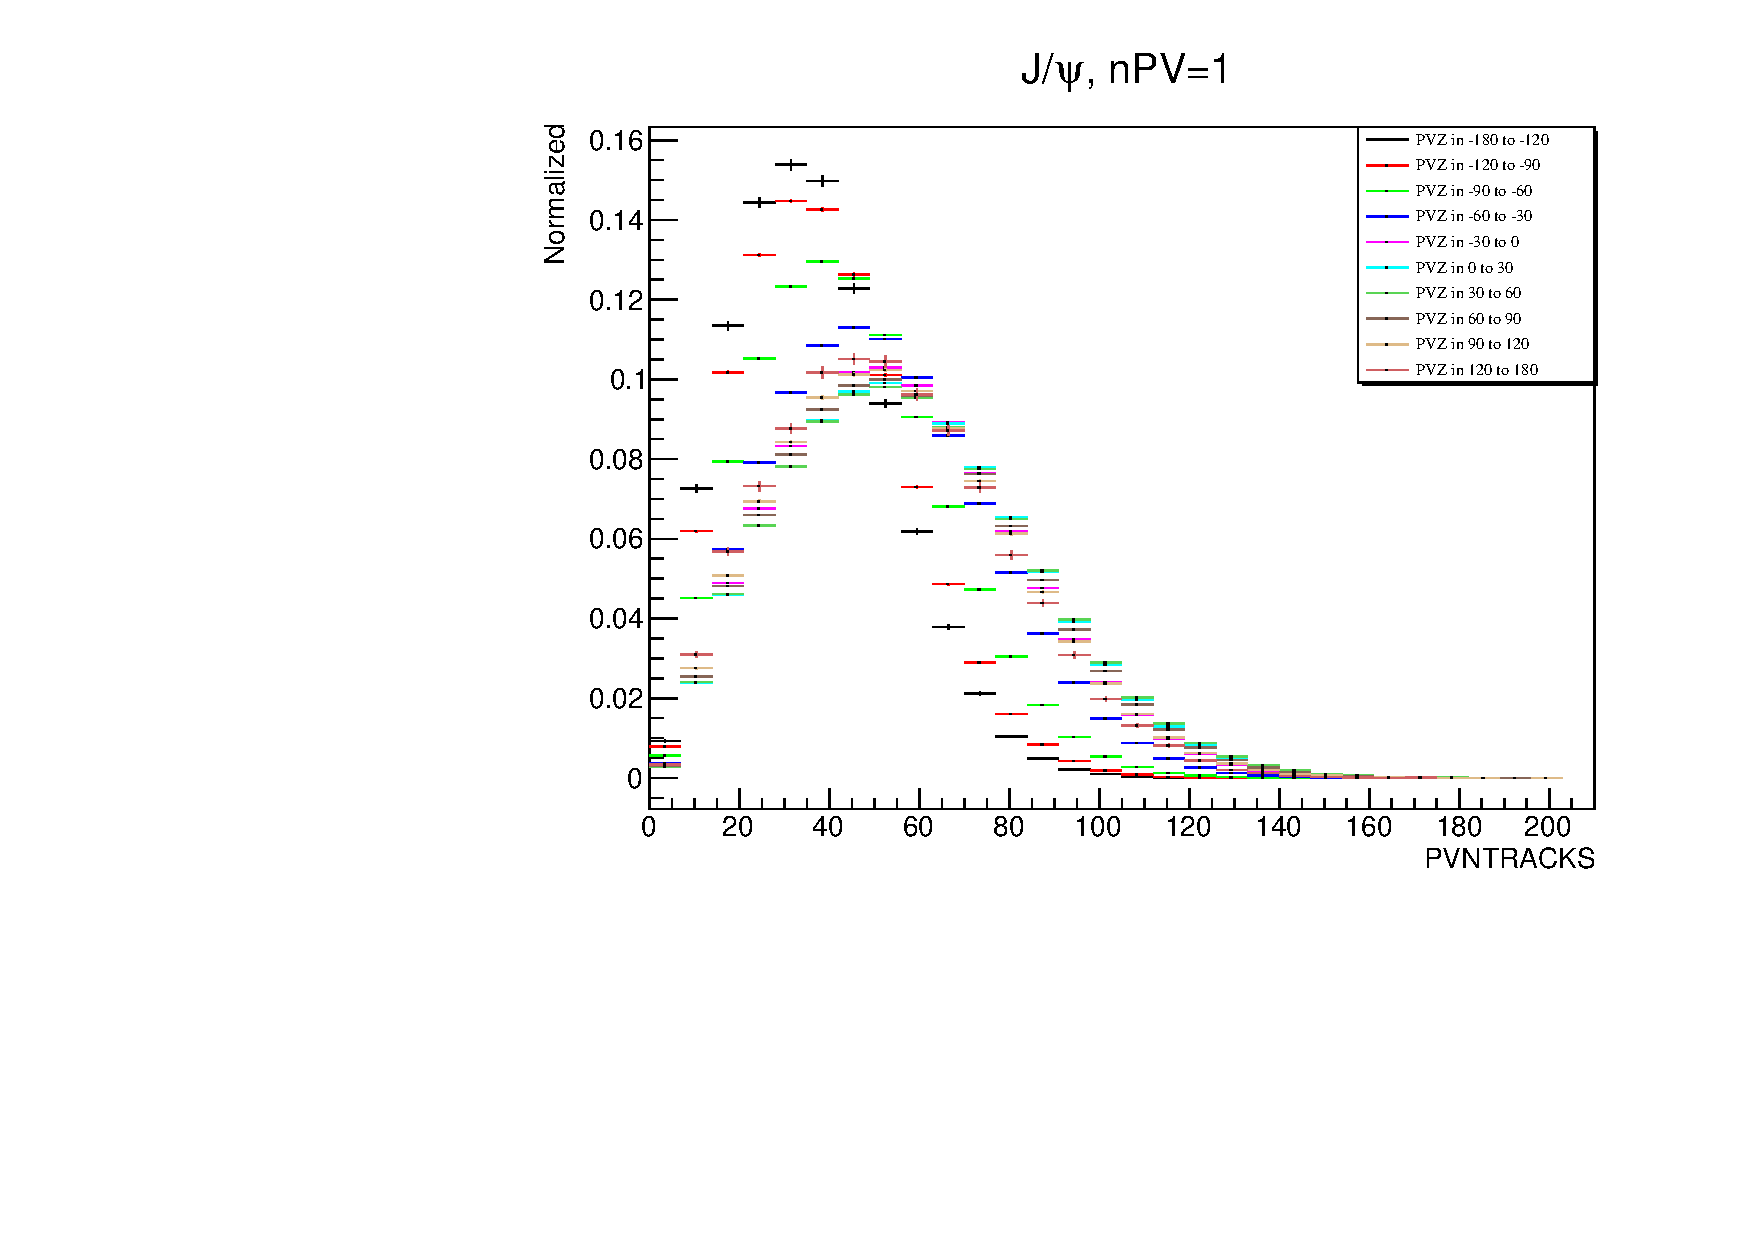
\includegraphics[width=0.49\linewidth]{Jpsi_PVZ_vs_PVNTRACKS}
      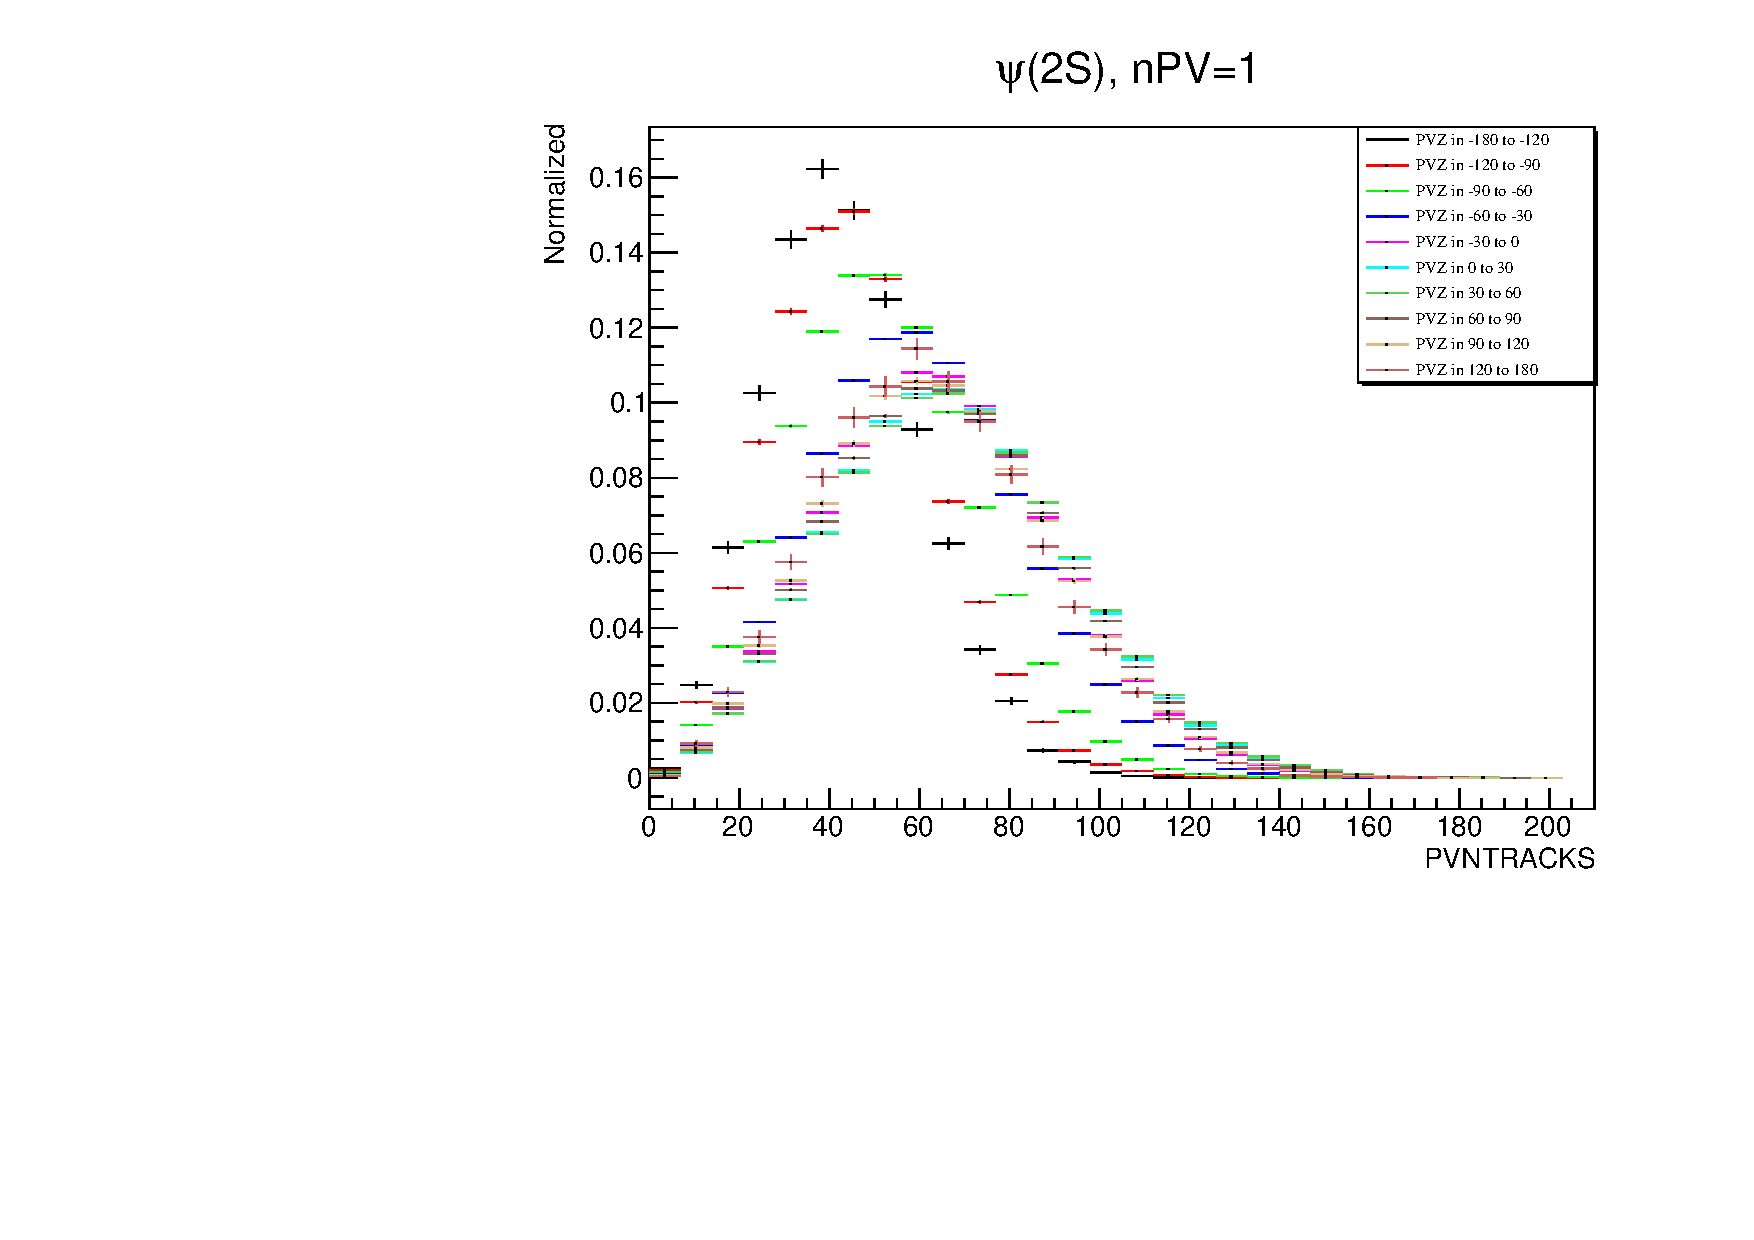
\includegraphics[width=0.49\linewidth]{Psi2S_PVZ_vs_PVNTRACKS}
      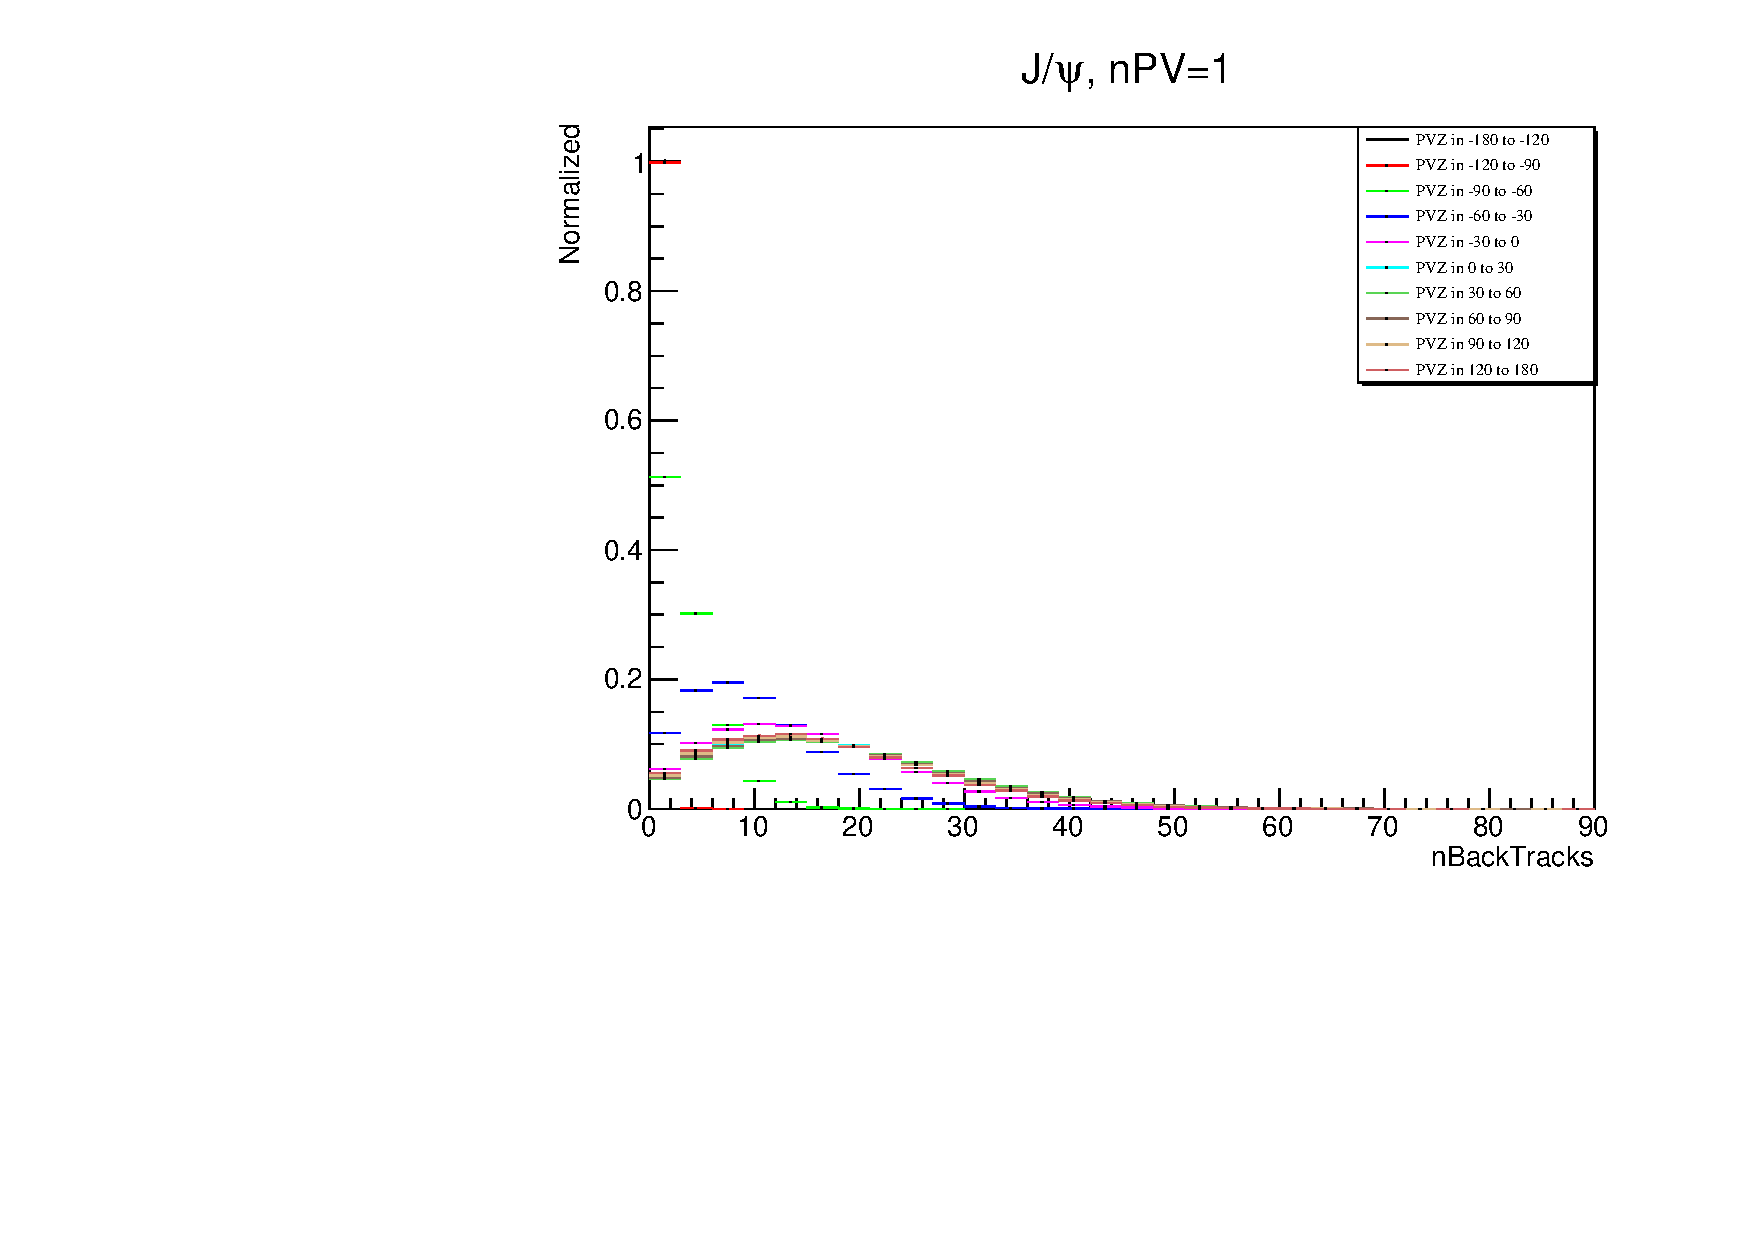
\includegraphics[width=0.49\linewidth]{Jpsi_PVZ_vs_nBackTracks}
      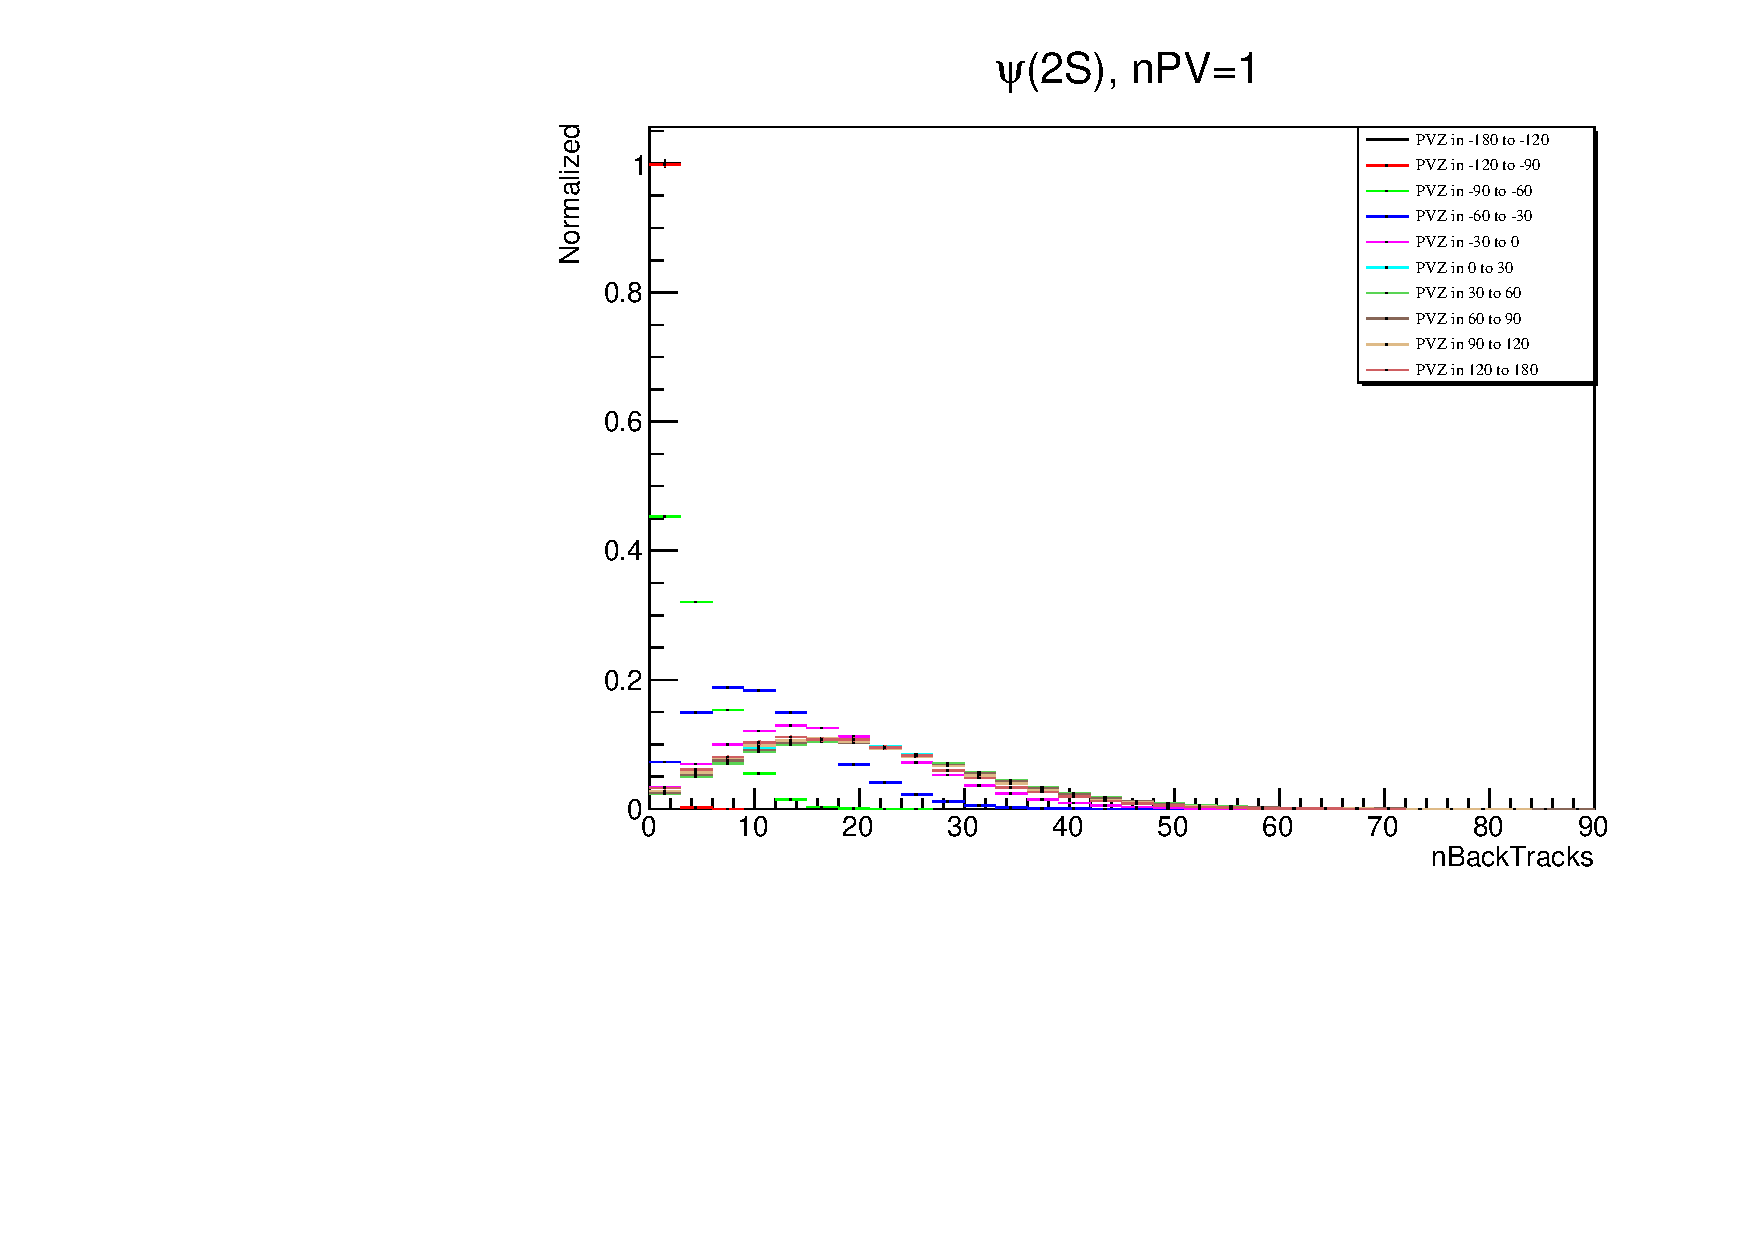
\includegraphics[width=0.49\linewidth]{Psi2S_PVZ_vs_nBackTracks}
      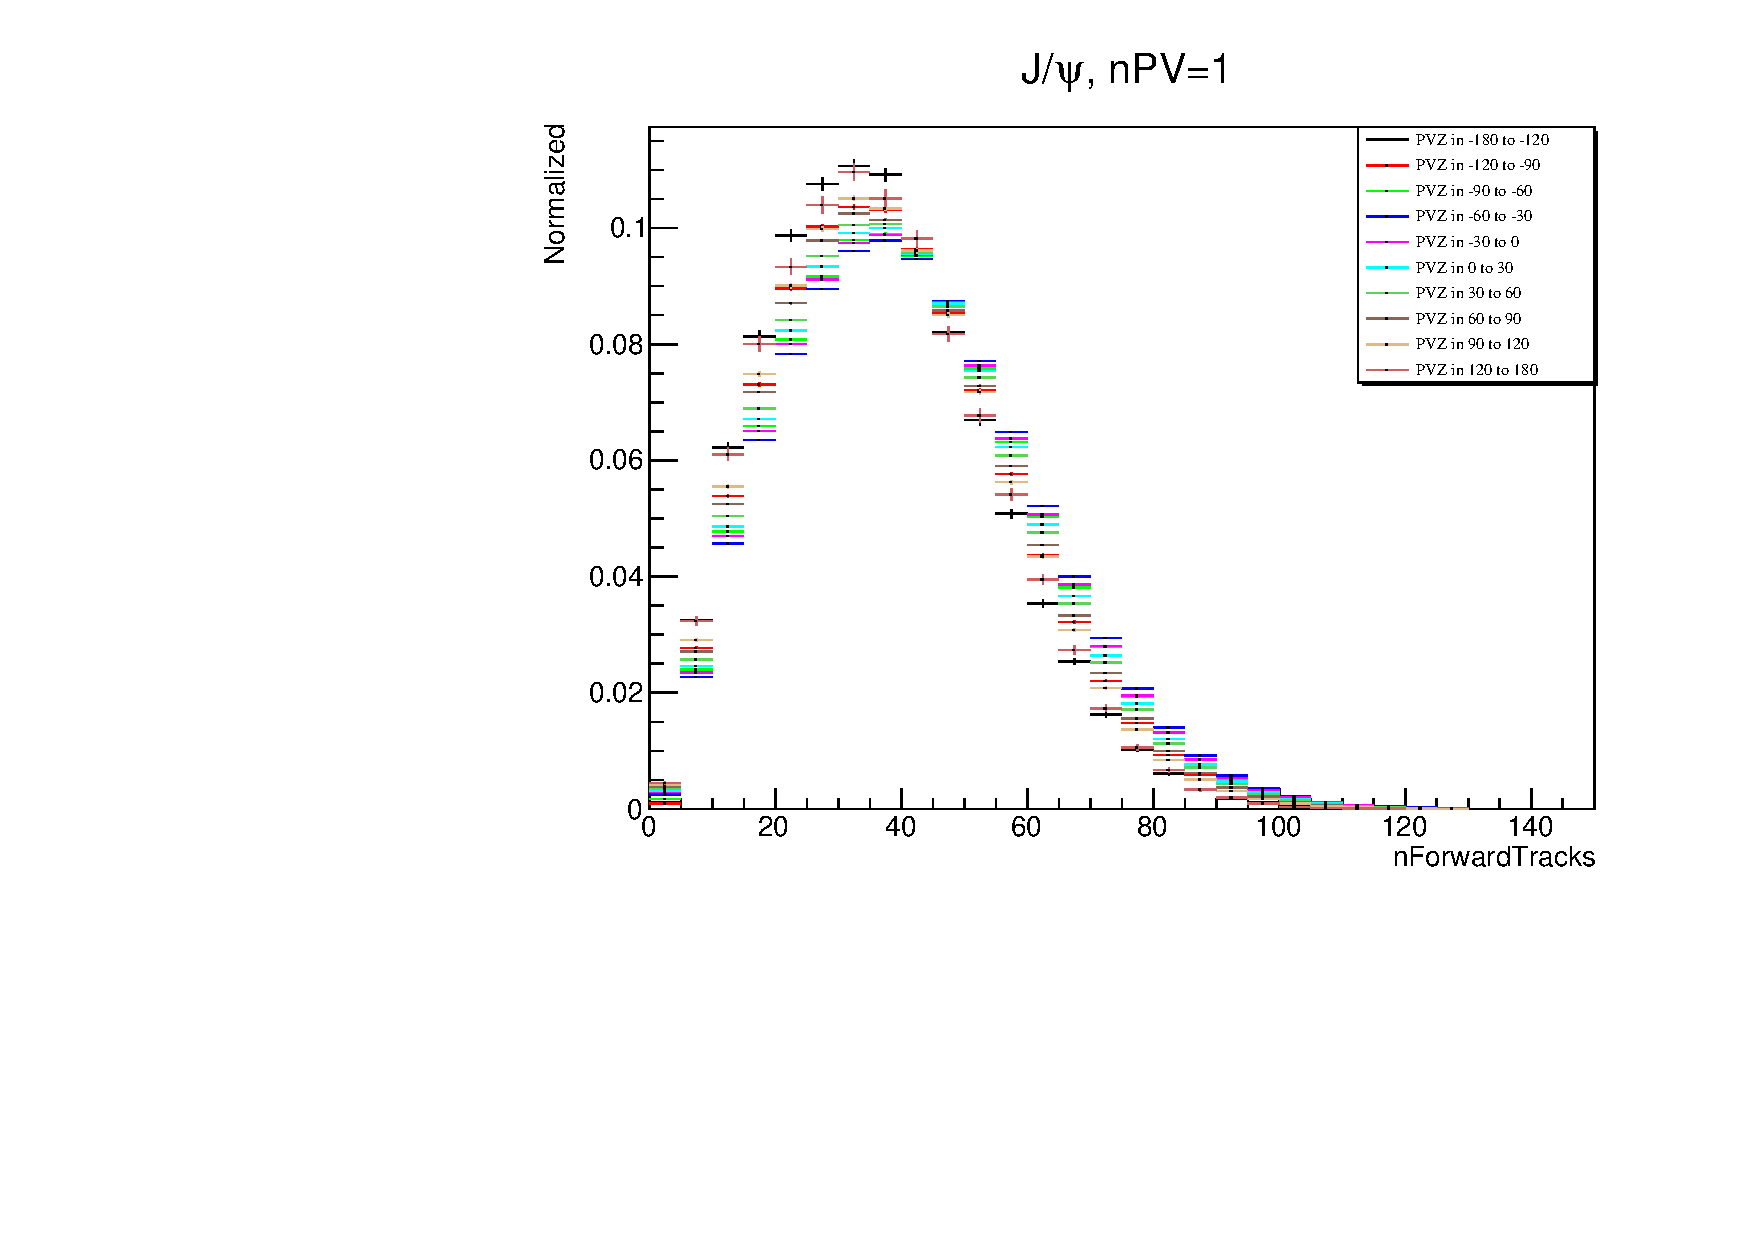
\includegraphics[width=0.49\linewidth]{Jpsi_PVZ_vs_nForwardTracks}
      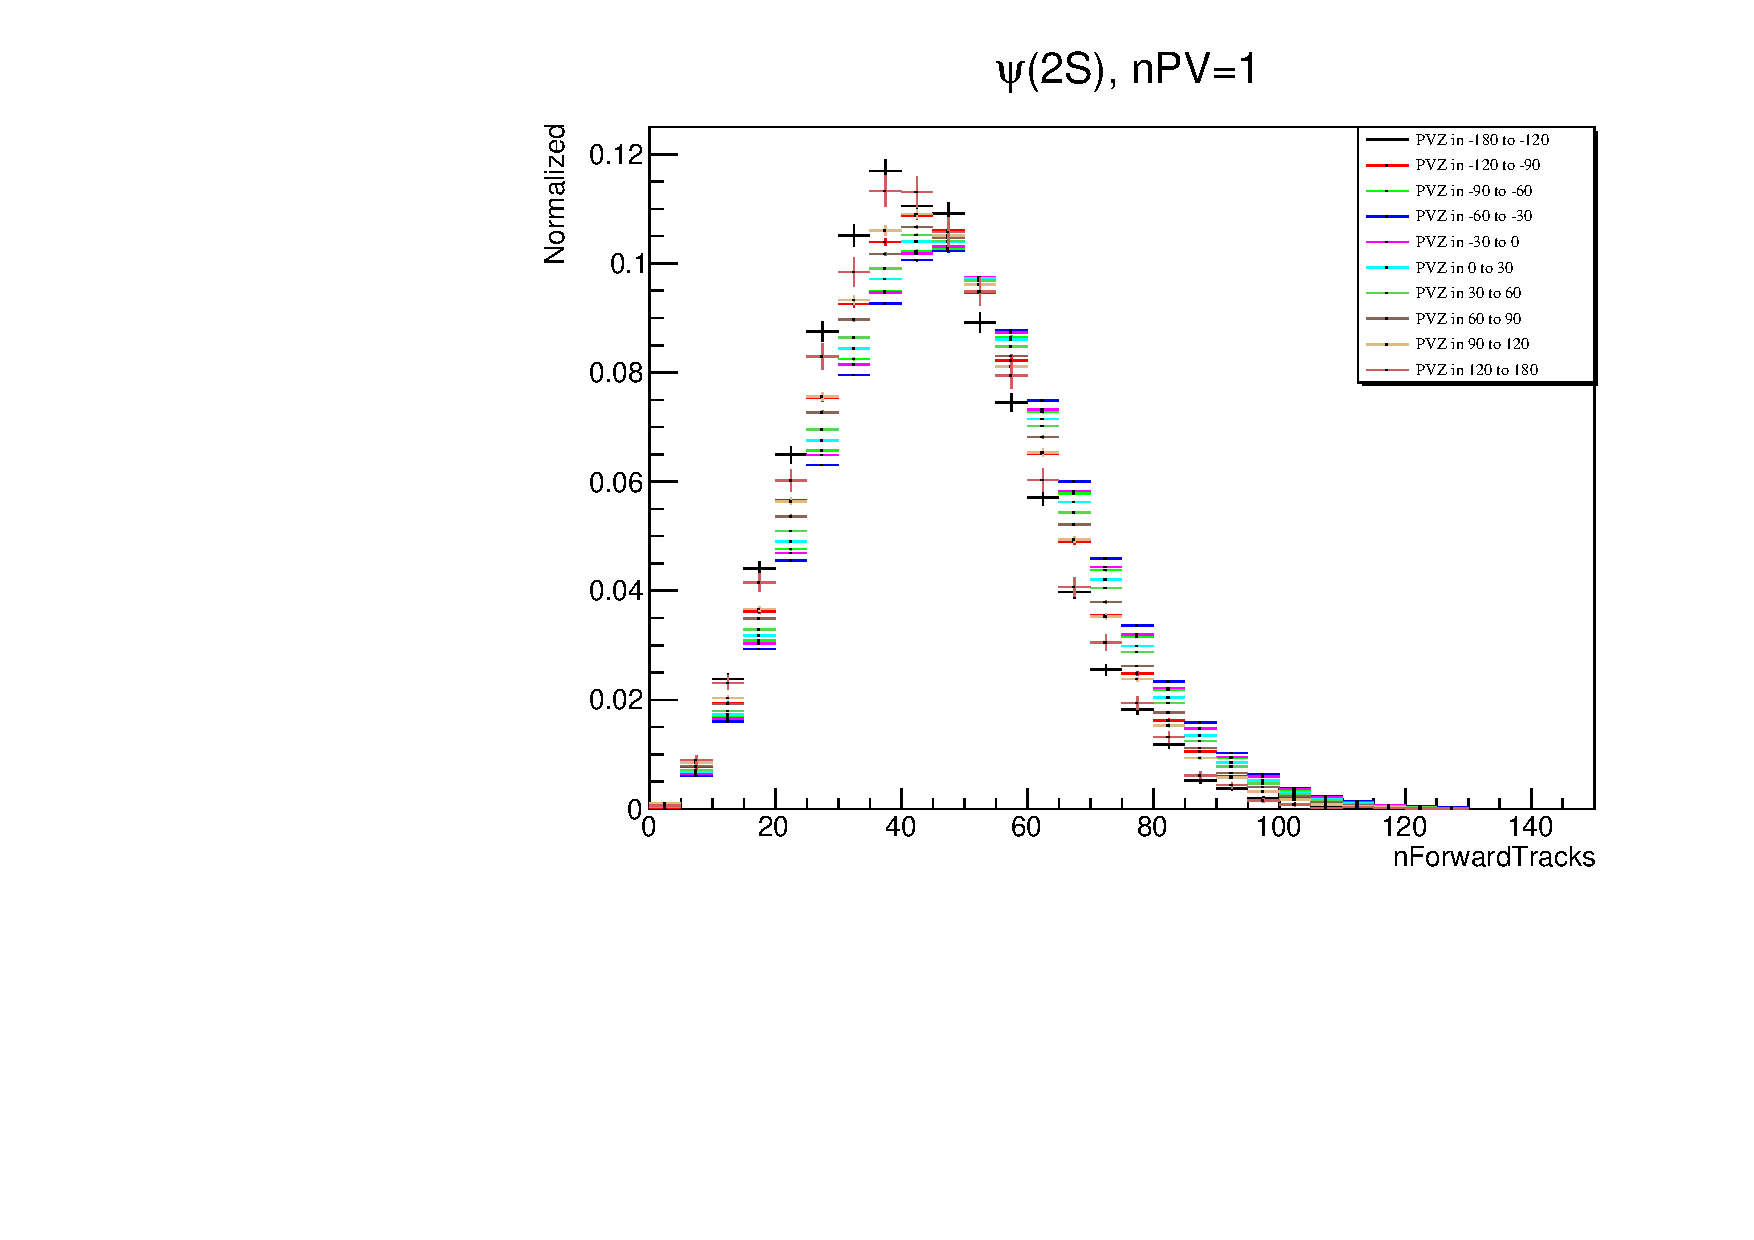
\includegraphics[width=0.49\linewidth]{Psi2S_PVZ_vs_nForwardTracks}
    \end{center}
    \caption{
    Distribution of PVNTRACKS, nBackTracks and nForwardTracks under nPVs $=1$ for $\jpsi$ (left) and $\psitwos$ (right). The clear deviation shows for $z_{\mathrm{PV}}$ smaller than a certain range so that we 
    subtract that part of data for equivalence of VELO acceptance.
      }
    \label{PVZvsPVNTRACKS}
  \end{figure}

\section{Ratio of Cross-Section Determination}
\label{Ratio of Cross-Section Determination}
\def\effTot{\ensuremath{\epsilon_{\mathrm{tot}}}\xspace}
\def\effTotJ{\ensuremath{\epsilon_{\mathrm{tot,\jpsi}}}\xspace}
\def\effTotP{\ensuremath{\epsilon_{\mathrm{tot,\psitwos}}}\xspace}
\subsection{Double Differential Cross-Section}
The determination of the double-differential production cross-section requires knowledge 
of the numbers of prompt and non-prompt signals of \jpsi and \psitwos in bins of the 
kinematic variables $y$ and $p_T$, and multiplicity bin. This is done by 
performing a simultaneous fit to the distributions of the dimuon invariant mass and the 
pseudo-proper time $t_z$ in each bin. The $t_z$ of promptly produced signals has 
zero lifetime, while the $t_z$ distribution for the non-prompt signal is 
approximately exponential as seen from the simulation. The pseudo-proper time $t_z$ allows us 
to statistically separate the prompt signal from that created in decays of b-hadrons.
The double differential cross-section for prompt $\jpsi$ and $\jpsi$ from-$b$ production in a given (\pt, y) 
bin with multiplicity in a certain range is defined as
\begin{equation}
    \frac{\deriv^2\sigma_{\jpsi}}{\deriv y\deriv \pt} 
    = \frac{N(\jpsi\rightarrow\mu^+\mu^-)}
           {\mathcal{L}\times\effTot\times \BR(\jpsi\rightarrow\mu^+\mu^-)\times\Delta y \times \Delta \pt}. 
  \label{CrossSecJ}
\end{equation}
And for $\psitwos$
\begin{equation}
    \frac{\deriv^2\sigma_{\psitwos}}{\deriv y\deriv \pt} 
    = \frac{N(\psitwos\rightarrow\mu^+\mu^-)}
           {\mathcal{L}\times\effTot\times k\cdot \BR(\psitwos\rightarrow e^+ e^-)\times\Delta y \times \Delta \pt}. 
  \label{CrossSecP}
\end{equation}  
where
\begin{itemize}
\item $N$ is either the number of prompt \psitwos or \psitwos from $b$-hadron signals of $\jpsi$ or $\psitwos$ reconstructed through the dimuon decay channel. They are obtained by the fits;
\item $\mathcal{L}$ is the integrated luminosity;
\item \effTot is the total efficiency in that particular $\pt-y$ bin with PVNTRACKS in a certain range, for both prompt and non-prompt and both  $\jpsi$ and $\psitwos$ respectively;
\item $k$ is the phase space factor which is assume to be unit under the assumption of lepton universality.
The lepton universality is a reasonable assumption under the current statistical precision;
\item $\BR(\jpsi\rightarrow\mu^+\mu^-)=(5.961\pm0.033)\%$ is the branching fraction of the decay $\jpsi\rightarrow \mu^+ \mu^-$, quoted from the PDG 2022 review~\cite{Workman:2022ynf}.
\item $\BR(\psitwos\rightarrow e^+e^-)=(7.93\pm0.17)\times10^{-3}$ is the branching fraction of the decay $\psitwos\rightarrow e^+ e^-$, quoted from the PDG 2022 review~\cite{Workman:2022ynf}. The dielectron branching fraction is used since it has a much smaller uncertainty than the dimuon one;
\item $\Delta\pt$ is the bin width of the transverse momentum;
\item $\Delta y$ is the bin width of the rapidity.
\end{itemize}
In the measurement of  modification of $b$ quark hadronization in high-multiplicity $pp$ collision at $\sqrt{s}=$ 13 TeV shows that, ratio of cross sections $\sigma_{B_s^0}/\sigma_{B^0}$ versus normalized multiplicity behaves differently according to the choices of multiplicity variable~\cite{LHCb:2022syj}. That motivates us to measure how the ratio changes with different multiplicity variables.
The following boundaries are used for the binning scheme of \pt, $y$ and different multiplicity variables. To remove the contribution from photon-production charmonium, we remove the production for $\pt<0.3\gevc$:
\begin{itemize}
\item $\pt$ boundaries [\gevc]: 0.3, 2, 4, 6, 8, 20; 
\item $y$ boundaries: 2.0, 2.8, 3.5, 4.5;
\item For multiplicity (each at a time)
\begin{itemize}
  \item PVNTRACKS: 4, 20, 45, 70, 95, 200. (At least 4 tracks required.)
  \item nBackTracks: 0, 8, 15, 22, 30, 80.
  \item nForwardTracks: 0, 12, 24, 36, 48, 130.
\end{itemize}  
\end{itemize}
There is a wider bin in high \pt and multiplicity region, and the scheme of $y$ is not exactly evenly distributed for the sake of significant signal numbers for fitting in each bin. And this binning scheme is common for both $\jpsi$ and $\psitwos$.
To see how charmonium suppression is affected by charged particle multiplicity, we normalize the ratio of production to see the trend. The multiplicity variables are normalized by their respective mean value from an unbiased data sample from the same year. Here we divide them by the mean values from NoBias data rather than just the mean values in their trigger lines is due to the fact that the trigger line may influence the distribution of charged particle multiplicity. So the x-coordinate represents 'how many times is the multiplicity to the mean value of multiplicity from NoBias data'. Since the multiplicity distributions in high-energy hadron collisions is a KNO variable~\cite {Koba:1972ng}, which is, after normalized, the distribution of a certain collision system has the same distribution of a certain multiplicity variable. By scaling we change the multiplicity variable as a scale of how many times the mean number of charged particle multiplicity, so that the results are compatible with other results.


\subsection{Ratio of Cross-Section}
In each multiplicity region, we have defined the double differential cross-section in kinetic bin $(\pt,y)$ above. 
Then the ratio of double differential cross-section is determined as follows
\begin{equation} 
    \frac{\sigma(\pt,y)_{\psitwos}}{\sigma(\pt,y,)_{\jpsi}} = 
    \frac{N_{\psitwos}(\pt,y,)}{N_{\jpsi}(\pt,y,)} \times
    \frac{\effTotJ(\pt,y)} {\effTotP(\pt,y)} \times 
    \frac{\mathcal{B}_{\jpsi \rightarrow \mu^+ \mu^-}}{k\times \mathcal{B}_{\psitwos\rightarrow e^+e^-}},
    \label{Rsingle}
    \end{equation}
where the bin widths for \pt and $y$ are canceled out, so as the luminosity term. While when calculating the ratio 
of differential cross-section, the bin widths of \pt and $y$ are no longer canceled out since the binning scheme 
is not uniform. Hence, the ratio of the cross-section is determined as follows,
\begin{equation} 
    \frac{\Sigma_{(\pt,y)}\sigma_{\psitwos}(\pt,y)}{\Sigma_{(\pt,y)}\sigma_{\jpsi}(\pt,y)} = 
    \frac{\Sigma_{(\pt,y)}(\Delta \pt \times \Delta y \times N_{\psitwos}(\pt,y) / \effTotP(\pt,y))}
    {\Sigma_{(\pt,y)}(\Delta \pt \times \Delta y \times N_{\jpsi}(\pt,y) / \effTotJ(\pt,y))} \times
    \frac{\mathcal{B}_{\jpsi \rightarrow \mu^+ \mu^-}}{k\times \mathcal{B}_{\psitwos\rightarrow e^+e^-}}.
\label{Rintegrated}
\end{equation}

In a small kinetic bin, the efficiency \effTot is assumed to be constant, and thus a single number with corresponding uncertainty is provided.
The efficiency for prompt non-prompt signals is calculated separately for $\jpsi$ and $\psitwos$. And since our scheme is not significantly small, a re-weight in \pt-$y$ spectrum is performed when calculating the efficiency.


\section{Signal Extraction}
\label{Signal Extraction}
The total number of $\jpsi$ and $\psitwos$ signals is determined from an extended unbinned maximum 
likelihood fit to the invariant mass distribution of the selected candidates. The fit models for both $\jpsi$ 
and $\psitwos$ are the same, which we consider the previous studies of $\jpsi$ production at 13 TeV~\cite{LHCb-PAPER-2015-037} 
and $\psitwos$ production at 13 TeV~\cite{LHCb:2019eaj}. The only strategy for both is as follows.

In the fit the component of the background is modelled with an exponential function
\begin{equation}
f_{\rm bkg}(m)=a_0e^{-p_0\cdot m}.
\end{equation}
The signal component is described by the sum of two Crystal Ball (CB) functions~\cite{Skwarnicki:1986xj}.
The CB function is defined as:
\begin{equation}
 f_{\mathrm{CB}}(m;\mu,\sigma,\alpha,n) = 
 \begin{cases} 
      %\frac{\Big(\frac{n}{|\alpha|}\Big)^n e^{-\frac{1}{2}\alpha^2}}{(\frac{n}{|\alpha|}-|\alpha|-\frac{m-\mu}{\sigma})^n} & \frac{m-\mu}{\sigma} < -|\alpha|\\
      \Big(\frac{n}{|\alpha|}\Big)^n e^{-\frac{1}{2}\alpha^2} (\frac{n}{|\alpha|}-|\alpha|-\frac{m-\mu}{\sigma})^{-n} & \frac{m-\mu}{\sigma} < -|\alpha|\\
   \exp\Bigg( -\frac{1}{2}\Big(\frac{m-\mu}{\sigma}\Big)^2\Bigg) & \frac{m-\mu}{\sigma}>-|\alpha|.
\end{cases},
\end{equation}
which combines a Gaussian core (described by the parameters $\mu$ and $\sigma$) and one tail on the left (described by the parameters $\alpha$ and $n$).
The tails in CB functions are used to model the radiative effects, which leads to more candidates with lower invariant masses.
Not all parameters of the CB functions are free when fitting data. 
Some parameters are fixed or parameterized.
For both $\jpsi$ and $\psitwos$, the two CB functions share one common mean value $\mu$ and have different widths $\sigma_1$ and $\sigma_2$, and $\alpha$ is parametrized from simulation as a function of the $\sigma$:
$\alpha=2.066\pm0.0085\sigma-0.00011\sigma^2$, which applies to both CB functions. Furthermore, for $\psitwos$ only, $\sigma_1$ and $\sigma_2$ are parameterized as a linear function: $\sigma_2=25.7+\sigma_1$ and the fraction of the narrower CB function is fixed at 0.96. 
For the tail parameters, $n$ is fixed to unity from physics~\cite{LefrancoisTalk}.
%is used for different kinematic bins of \psitwos.
Therefore, there are merely two free parameters for the signal shape, $\mu$ and $\sigma_1$. The strategy followed the previous study of $\jpsi$ and $\psitwos$ production at 13 TeV~\cite{LHCb-PAPER-2015-037,LHCb:2019eaj}.
The invariant mass fit is performed in each $\pt-y$ and PVNTRACKS bin of the candidate.

\subsection{Determination of the prompt and detached signal yields}
\label{sec:MassTzFit}
To determine the signal yields of prompt and from-\bquark components separately, the $t_z$ distribution is used.
In each kinematic and multiplicity bin, an unbinned extended maximum likelihood fit to the two-dimension distributions of invariant mass $m(\mumu)$ and $t_z$ is performed to separate prompt component from that from \bquark.

At the generator level, the $t_z$ distribution of the prompt component is a Dirac delta function, $\delta(t_z)$, while that from $\bquark$ follows an exponential function as seen from simulation. 
For \jpsi and \psitwos signals, the detector resolution is taken into account by convolving a resolution function, which is described by the sum of two Gaussian functions,
\begin{equation}
f_\mathrm{resolution}(t_z;\mu,S_1,S_2,\beta) = \frac{\beta}{\sqrt{2\pi}S_1\sigma} e^{-\frac{(t_z-\mu)^2}{2S_1^2\sigma^2}}
+\frac{1-\beta}{\sqrt{2\pi}S_2\sigma} e^{-\frac{(t_z-\mu)^2}{2S_2^2\sigma^2}}.
\end{equation}
The parameter $\sigma$ is the event-by-event uncertainty of $t_z$, calculated by combining the estimated uncertainties of the \jpsi and \psitwos decay vertex and the associated PV.
Besides,$S_1$ and $S_2$ are two scale factors to correct the non-perfect estimation of the $t_z$ uncertainty, the parameter $\mu$ is the bias of the $t_z$ measurement, and $\beta$ is the fraction of one of the two Gaussians. 
In the fitting procedure, all the resolution parameters are floated.
For some (\pt,$y$, PVNTRACKS) bin, the count for signal yield for \psitwos or \jpsi is significantly low that fit will fail for too many free parameters, and we may set $\beta=0$, which is, only one Gaussian function is used to describe the resolution. 

It is possible that the reconstructed candidate is associated with a "wrong" PV. 
This can happen either because the real PV that produces the candidate failed to be reconstructed, and the candidate was associated with the nearest reconstructed PV in the event, or because a wrong PV is accidentally close to the candidate.
For the latter case, the positions of the reconstructed and the true PV are correlated, which results in a Gaussian-like $t_z$ distribution with a width much larger than the detection resolution. 
This effect can be described by adding a third Gaussian with a much larger width than the resolution function. 
However, it is found from simulation that including the wide Gaussian in the resolution does not change the fitted parameters significantly because the fraction of this component is quite small, $\leq 1\%$ as seen from studies in Ref.\cite{LHCb-PAPER-2015-037}.
Therefore, the third wide Gaussian is not used in the fit function.
For the former case that the true PV is not reconstructed, the true PV and wrongly associated PV are not correlated, which results in a long tail in the $t_z$ distribution that can be modeled using the next-event method for both \jpsi and \psitwos. 
The next-event method is applied directly on data sample. 
The next-event pseudo-proper time, $t_z^\mathrm{next}$, for each candidate, is calculated combining the candidate with the closest PV of another (next) event as
\begin{equation}
t_z^\mathrm{next}=\frac{(z_{\mu\mu}-z_\mathrm{PV}^\mathrm{next})\times m_{\mu\mu}}{p_z},
\end{equation}
where $z_\mathrm{PV}^\mathrm{next}$ is the $z$-coordinate of the nearest PV of the next selected event. 
The tail distribution is extracted in each bin separately and not convolved with resolution functions since the distribution is much wider than the resolution and very smooth in the whole $t_z$ region.
It should be noted that since the requirement of PV reconstruction is loose, using at least 4 VELO tracks, the probability to reconstruct the true PV is very high ($>99\%$). 

The candidates in the mass sidebands, where $m_{\mumu}$ is at least 60 $\mevc$ away from the mass of $\jpsi$ and $\psitwos$, are used as the background control sample to model the $t_z$ distribution of the background.
The background control sample consists of random combinations of muons from semi-leptonic $\bquark$ and $\cquark$ decays, which tend to produce positive $t_z$ values, as well as mis-reconstructed tracks from decays-in-flight of kaons and pions, which contribute both to positive and negative $t_z$ values.
The $t_z$ distribution of the background is therefore modeled with an empirical function, composed of a Dirac delta function and five exponentials (three for positive $t_z$ and two for negative $t_z$, with one positive $t_z$ and one negative sharing the same slope parameter). 
This function is convolved with the sum of two Gaussian functions as a resolution function, which has different parameters as for signals,\footnote{The uncertainty on the background vertex is usually worse than that for the signal vertex. } ,
\begin{align}
f_\mathrm{background} &=
\left[(1-f_1-f_2-f_3-f_4)\delta(t_z)+\theta(t_z)(\frac{f_1}{\tau_1}e^{-t_z/\tau_1}+\frac{f_2}{\tau_2}e^{-t_z/\tau_2})\right.
\nonumber\\
&\left. +\theta(-t_z)\frac{f_3}{\tau_3}e^{t_z/\tau_3}+\frac{f_4}{2\tau_4}e^{-|t_z|/\tau_4}
\right]\ast \left(\frac{\beta'}{\sqrt{2\pi}S^{'}_1\sigma} e^{-\frac{(t_z-\mu)^2}{2S^{'2}_1\sigma^2}}
  +\frac{1-\beta'}{\sqrt{2\pi}S^{'}_2\sigma} e^{-\frac{(t_z-\mu)^2}{2S^{'2}_2\sigma^2}}\right). 
\label{eq:TzBKG}
\end{align}
The parameters in Eq.~\ref{eq:TzBKG} are determined by fitting the $t_z$ distribution of background control sample defined above (in each kinematical bin of \jpsi and \psitwos), and are fixed for the final fits. 
In Fig.~\ref{fig:TzBKG}, the $t_z$ distribution of the background in the kinematic range $\pt\in[2,4]\gevc$, $y\in[2.0,2.8]$ and PVNTRACKS $\in[20,40]$ is shown, superposed by a fit using Eq.~\ref{eq:TzBKG}. 
%In Tables \ref{tab:tzbkgFitResults0}, \ref{tab:tzbkgFitResults1}, \ref{tab:tzbkgFitResults2}, \ref{tab:tzbkgFitResults3} and \ref{tab:tzbkgFitResults4}, all the background parameters in $t_z$ fits are given in each kinematic bin. 
%%%%%%%%%%%%%%%%%%%%%%%%%%%%%%%%%%%%%%%%%%%%%%%%%%%%%%%%%%%
\begin{figure}[!tbp]
   \begin{center}
     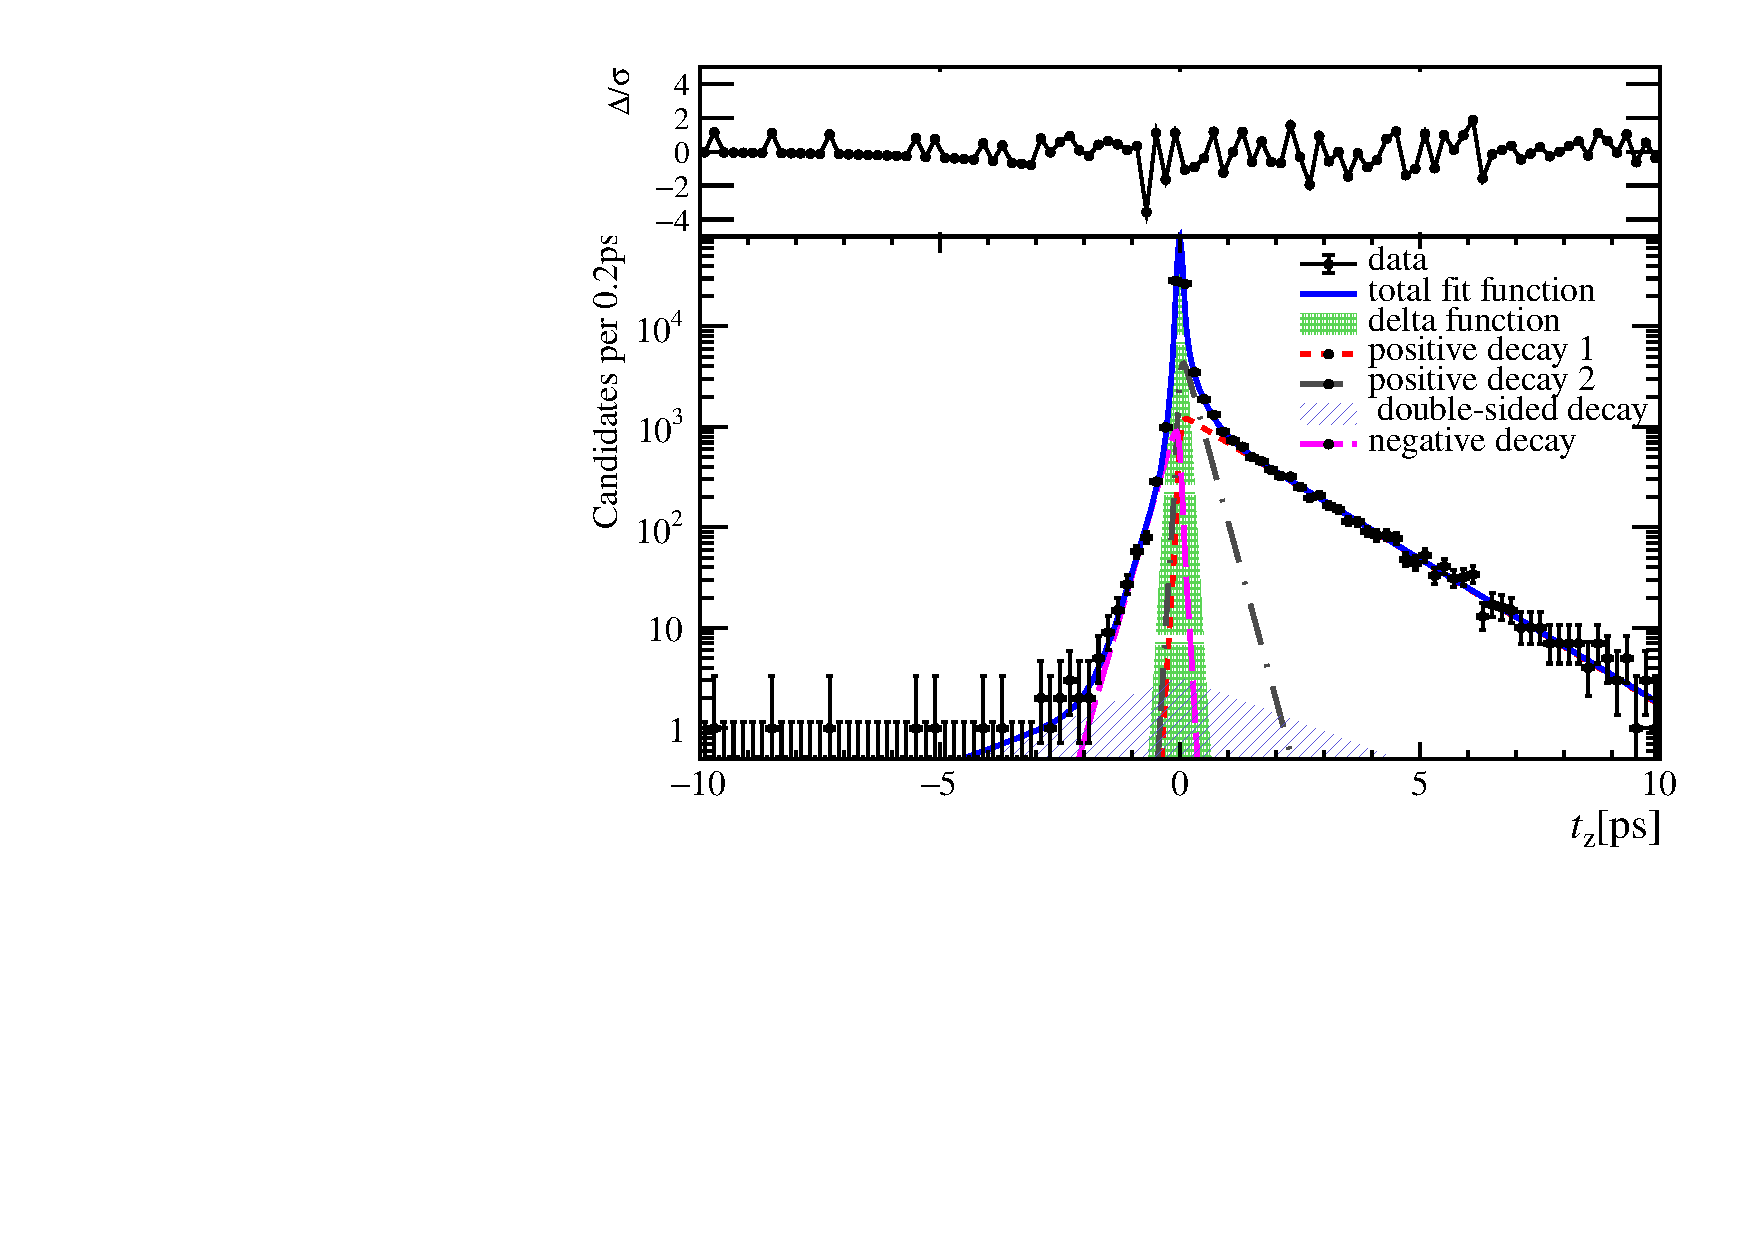
\includegraphics[width=0.49\linewidth]{pdf/Jpsi/Tzbkg/n2y1pt2}
     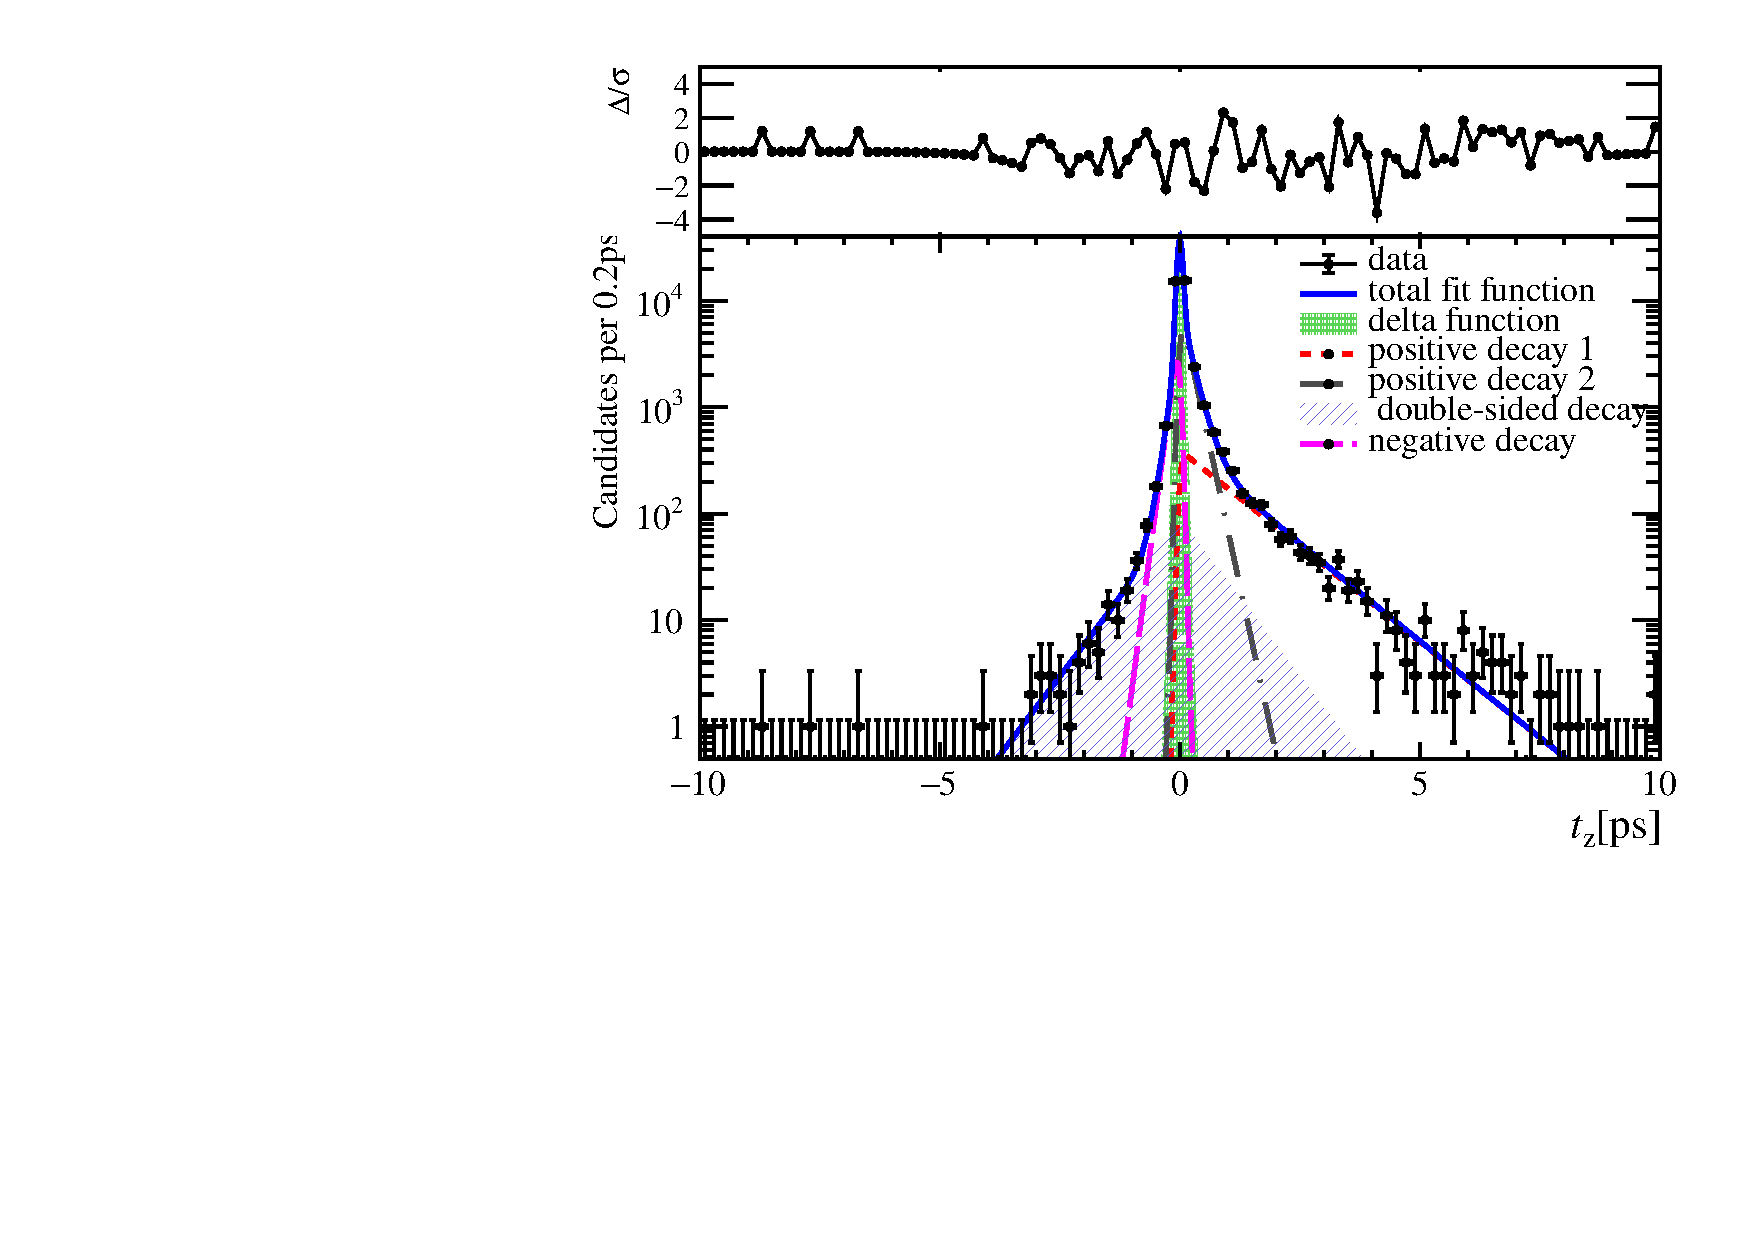
\includegraphics[width=0.49\linewidth]{pdf/Psi2S/Tzbkg/n2y1pt2}
     \vspace*{-0.5cm}
   \end{center}
   \caption{
     $t_z$ background fit for PVNTRACKS from 20 to 40, y from 2 to 2.8, and pt from 2$\gevc$ to 4 $\gevc$. The left is that of $\jpsi$ and the right is of $\psitwos$.
     }
   \label{fig:TzBKG}
 \end{figure}
%%%%%%%%%%%%%%%%%%%%%%%%%%%%%%%%%%%%%%%%%%%%%%%%%%%%%%%%%%
In total, the eventual function for the $t_z$ fit is:
\begin{align}
F_{t_z}(t_z;n_{\mathrm{prompt}},n_{tail},n_{\mathrm{bdecay}},n_\mathrm{bkg},\mu,S_1,S_2,\beta,\tau_b)&   \nonumber \\
      =\left(n_{\mathrm{prompt}}\delta(t_z)+\frac{n_{\mathrm{bdecay}}}{\tau_b}e^{-t_z/\tau_b}\right)\ast f_\mathrm{resolution}(t_z;\mu,S_1,S_2,\beta)
      &+n_{\mathrm{tail}} f_\mathrm{tail}(t_z)+n_\mathrm{bkg}f_\mathrm{background}(t_z), \label{eq:FinalTz}
\end{align}
where $n_\mathrm{bkg}$, $n_{\mathrm{prompt}}$, $n_{\mathrm{bdecay}}$ and $n_{\mathrm{tail}}$ are the number of background, prompt components, components from $\bquark$ and wrong PV events, respectively. 

Because the requirement of the PV reconstruction is loose, and the PV is not refitted by removing the VELO segments of the muon tracks, it is reasonable to assume that prompt components and components from $\bquark$ have equal probability to be assigned with a wrong PV.
Therefore, the fractions of the prompt and from $\bquark$ components in $n_{\mathrm{tail}}$ is equal to the fraction $\frac{n_{\mathrm{prompt}}}{n_{\mathrm{bdecay}}+n_{\mathrm{prompt}}}$ and $\frac{n_{\mathrm{bdecay}}}{n_{\mathrm{bdecay}}+n_{\mathrm{prompt}}}$. 
Even if the shape is extracted from data including the background candidate, the fit result $n_{\mathrm{tail}}$ should only contain prompt and non-prompt signals. First, the shape of the PDF due to the wrong-PV effect should be the same no matter from which sample we extract it. Then, 
the wrong-PV effect for background candidates should be merged in the background PDF, which means the $n_{\mathrm{tail}}$ part in the total PDF should be specifically for signal candidates.
And in this analysis, we only care about the ratio of prompt and from $\bquark$, where $n_{tail}$ in each kinetic bin and multiplicity bin accounts for about $0.1\%$ of $n_{\mathrm{bdecay}}+n_{\mathrm{prompt}}$, which results in an even more negligible influence on the ratio in Sec~\ref{Ratio of Cross-Section Determination}. 
In this case, we can ignore the subtle contribution to $n_{\mathrm{bdecay}}$ and $n_{\mathrm{prompt}}$ from $n_{tail}$. 

The two-dimensional fit to the invariant mass and the lifetime in the kinematic range $4\gevc<\pt<6\gevc$, $2.0<y<2.8$ 
and multiplicity bin 20$\leq$PVNTRACKS$<$40 is shown in Fig.~\ref{fig:2Dtz}, with the red shaded area being prompt components, and the cyan shaded area being components from $\bquark$, 
the dots with vertical error bar are data points, the violet dashed lines are the combinatorial background, the green dashed lines are the components by wrong PV (which are invisible in the graph of projection on mass) and 
the blue lines are the total fit functions.
During the $t_z$-mass combined fitting procedure, the parameters of mass signal shape ($\mu_{mass}$, $\sigma_{mass}$, $p_{0}$) are floated within a certain times of their uncertainties from the 1D mass fit for the final fits of \jpsi. While for \psitwos, due to the limitation of number of candidates, the parameters are fixed. According to the comparison of two fitting strategies upon \jpsi, no significant difference between errors of prompt and non-prompt signals are observed (~$0.1\%$).
%The $t_z$-mass combine fitted value $\beta$ (fraction of first Gaussian of signal resolution function),  $1000*\mu_{t_z}$ (bias of $t_z$ distribution), $S(1,2)_{t_z}$ ($\sigma_{1,2}$ of first/second Gaussian resolution function convolved with the $t_z$ function), $\tau_b$(effective $b$-hadron lifetime), $n_\mathrm{bkg}$, $n_{prompt}$ (number of prompt \psitwos), $n_{b-decay}$ (number of \psitwos-from-\bquark) and $n_{tail}$ (number of events in tail) are given in Tables\ref{tab:FitResults0}, \ref{tab:FitResults1}, \ref{tab:FitResults2}, \ref{tab:FitResults3} and \ref{tab:FitResults4}. 

 %%%%%%%%%%%%%%%%%%%%%%%%%%%%%%%%%%%%%%%%%%%%%%%%%%%%%%%%%%%
 \begin{figure}[!tbp]
   \begin{center}
     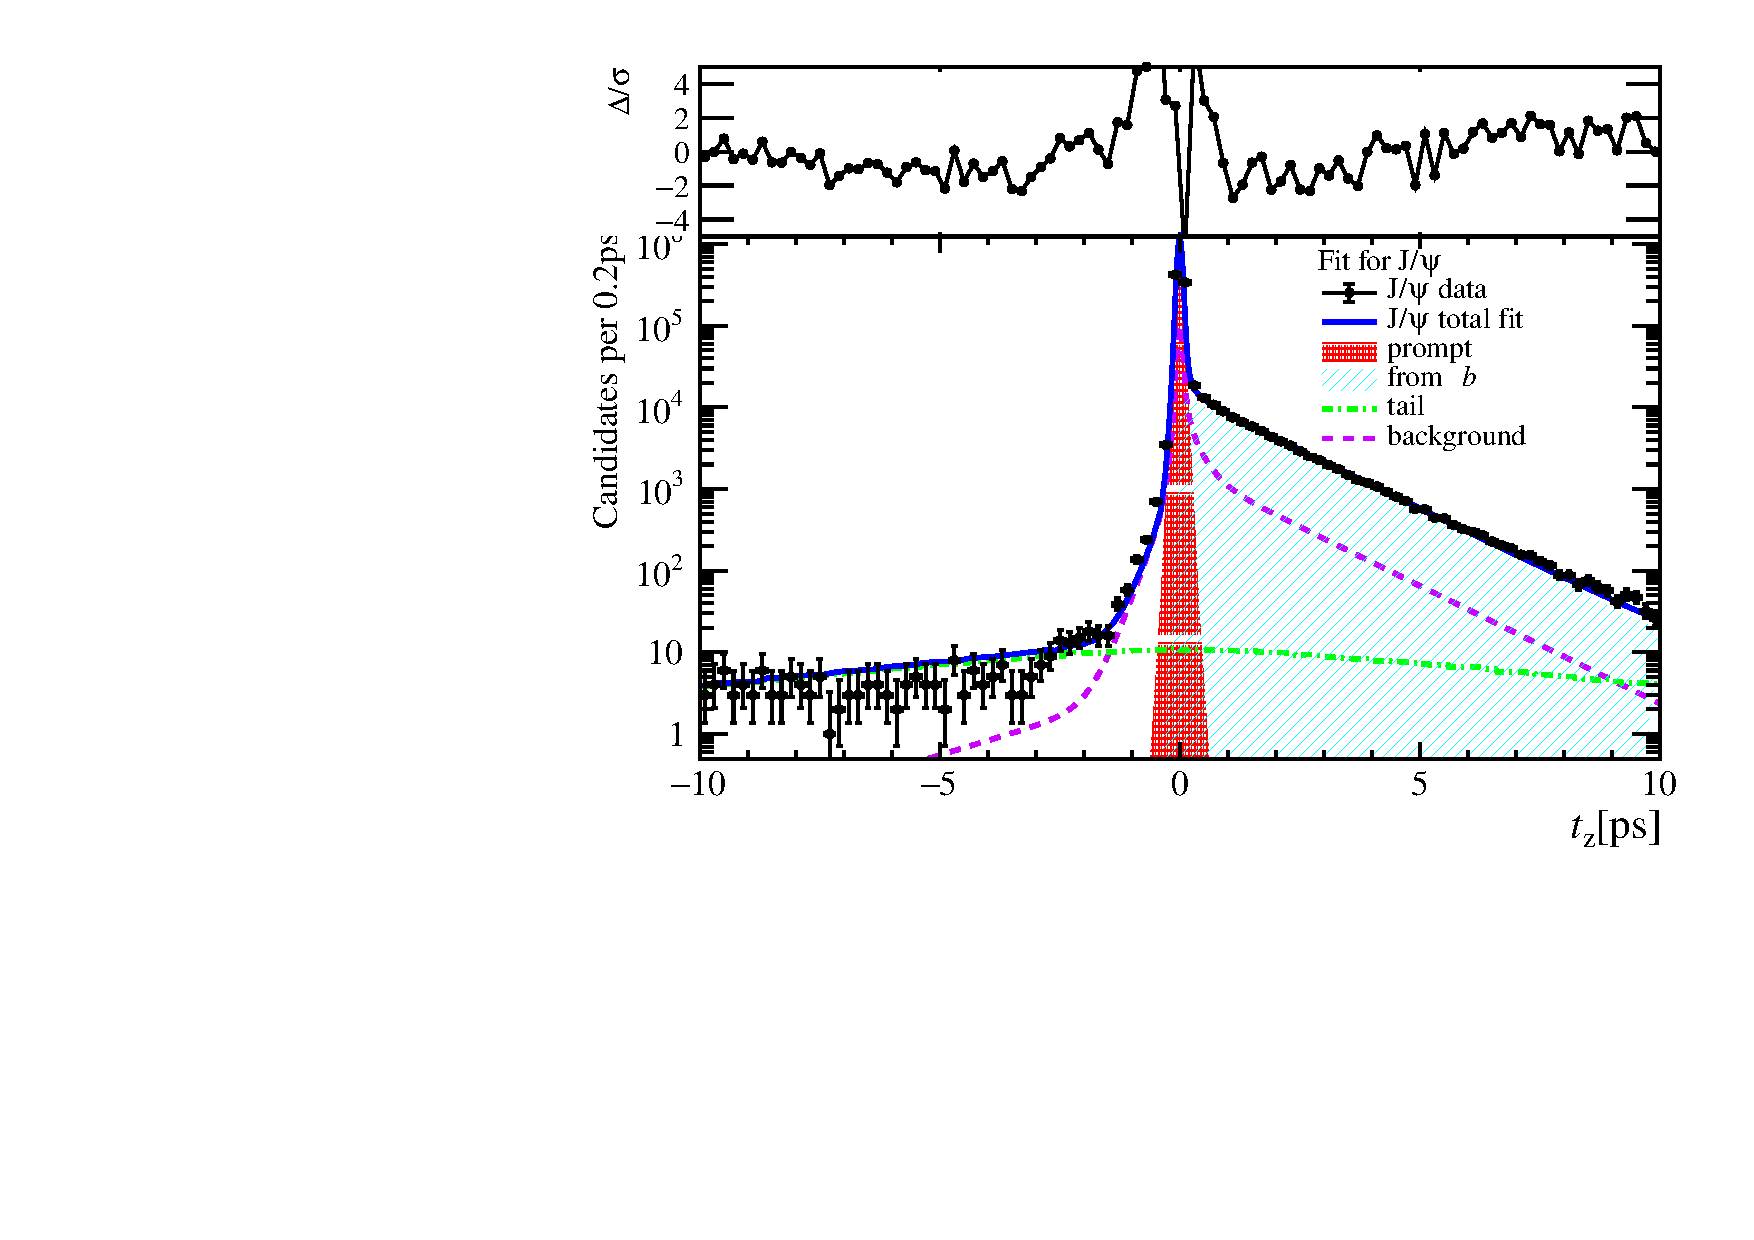
\includegraphics[width=0.49\linewidth]{pdf/Jpsi/2DFit/n2y1pt2.pdf}
     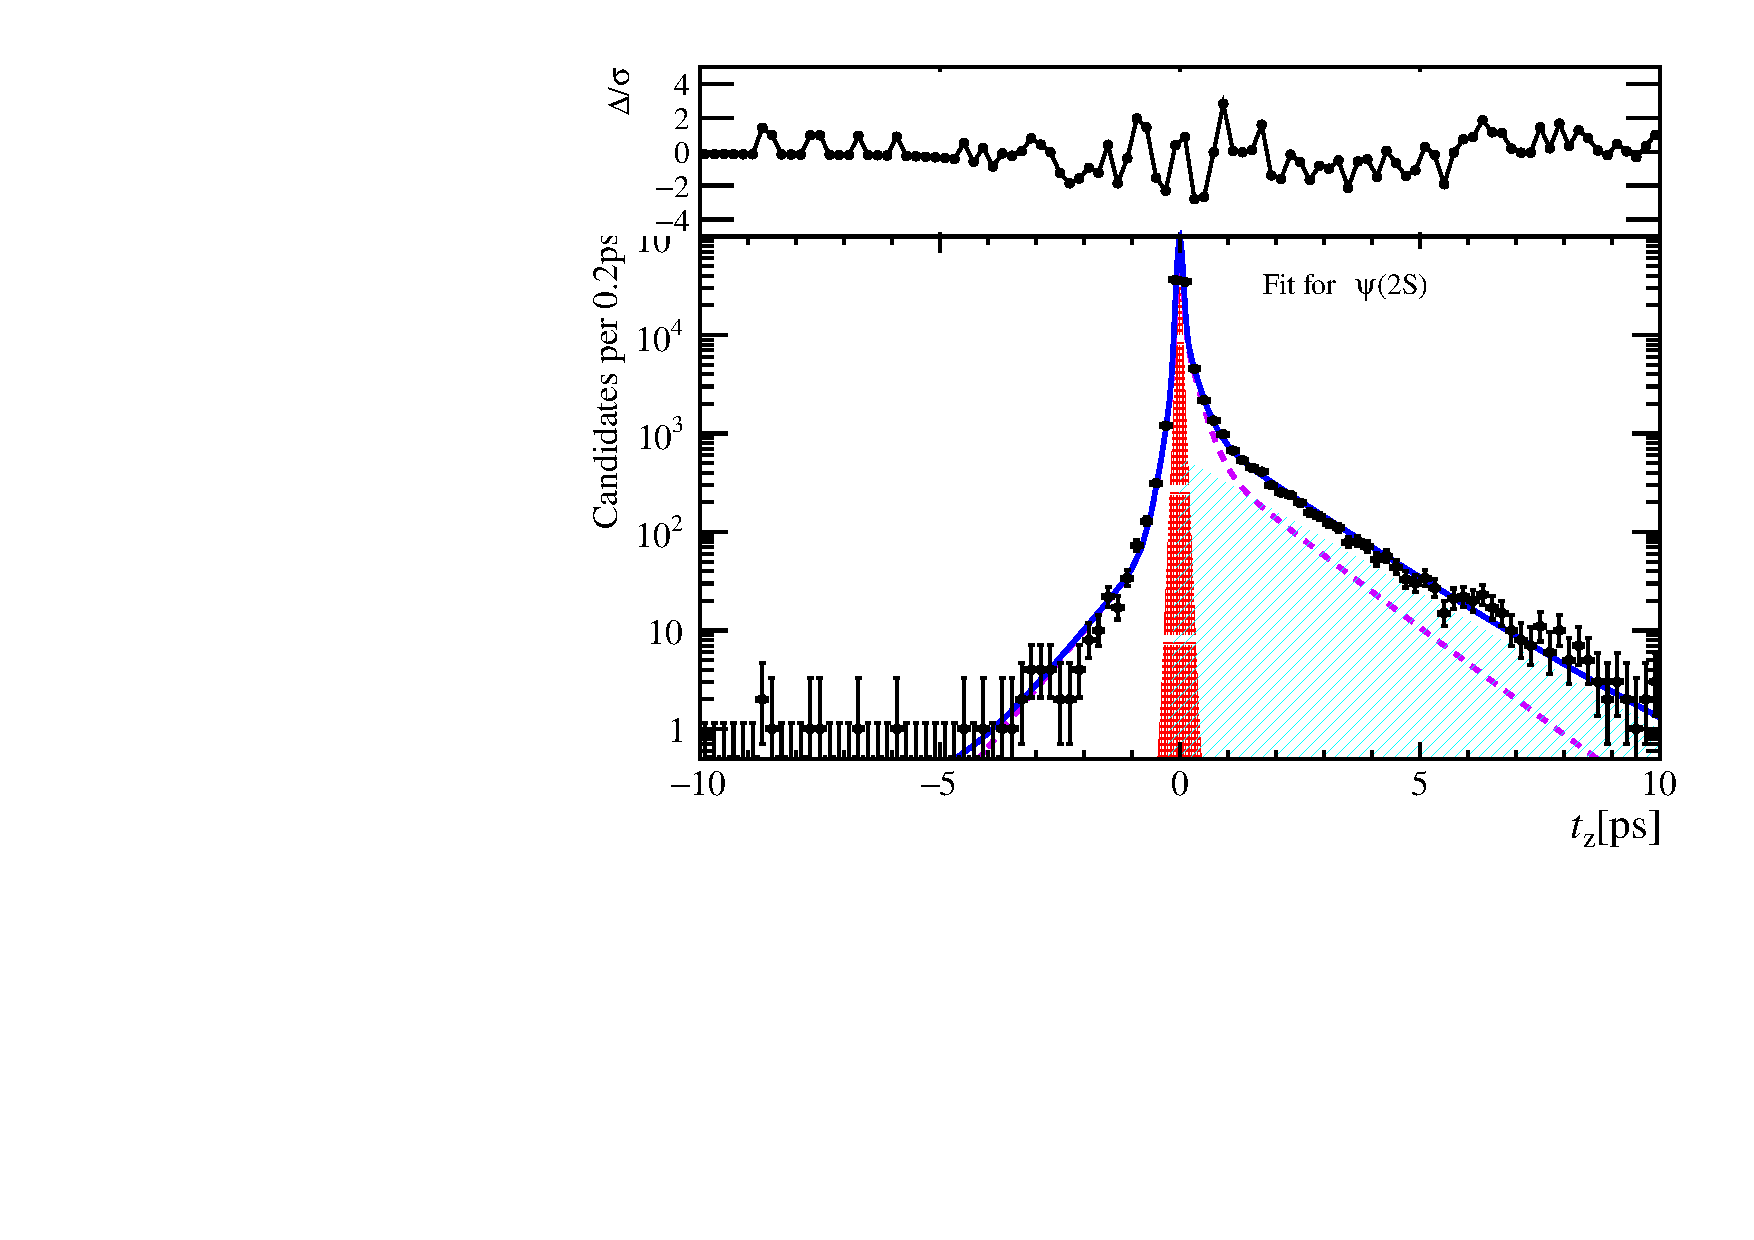
\includegraphics[width=0.49\linewidth]{pdf/Psi2S/2DFit/n2y1pt2.pdf}
     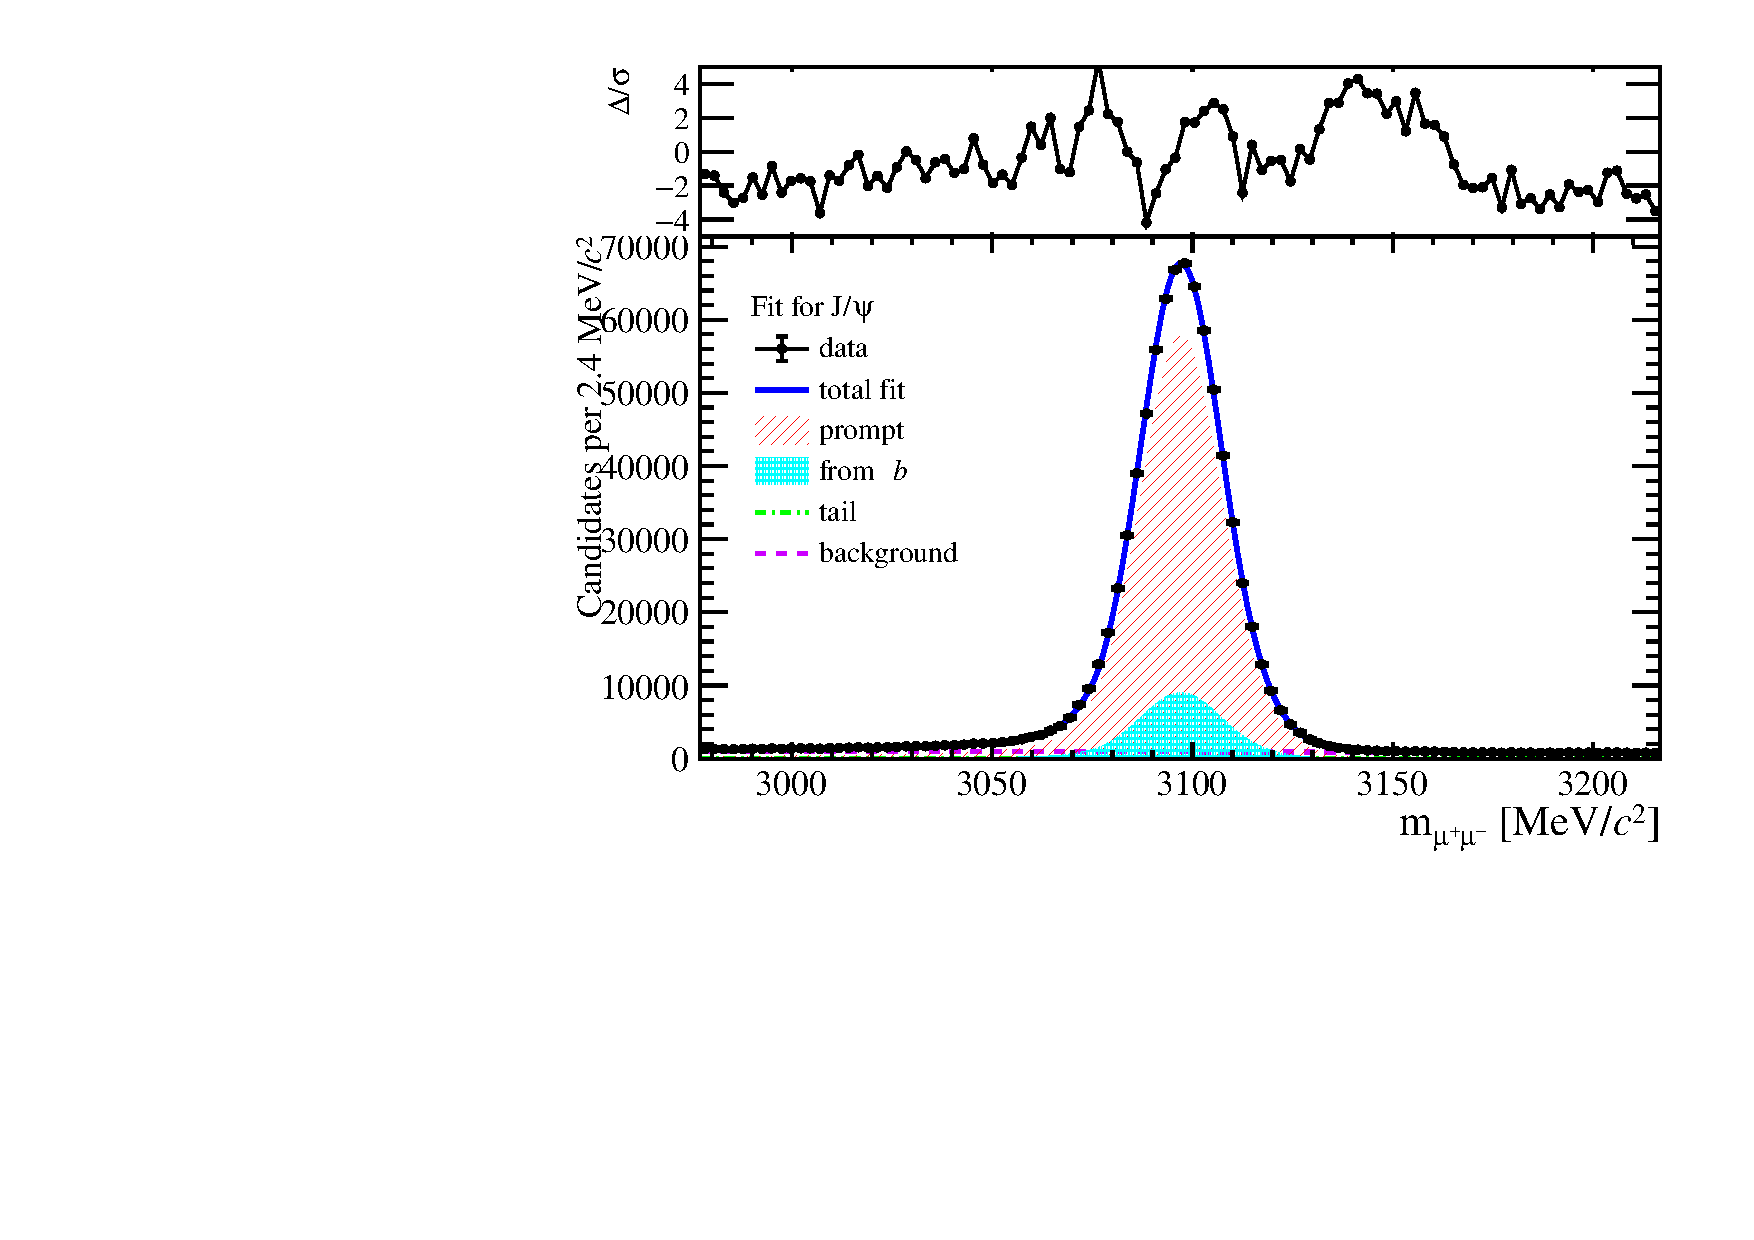
\includegraphics[width=0.49\linewidth]{pdf/Jpsi/drawmass/n2y1pt2.pdf}
     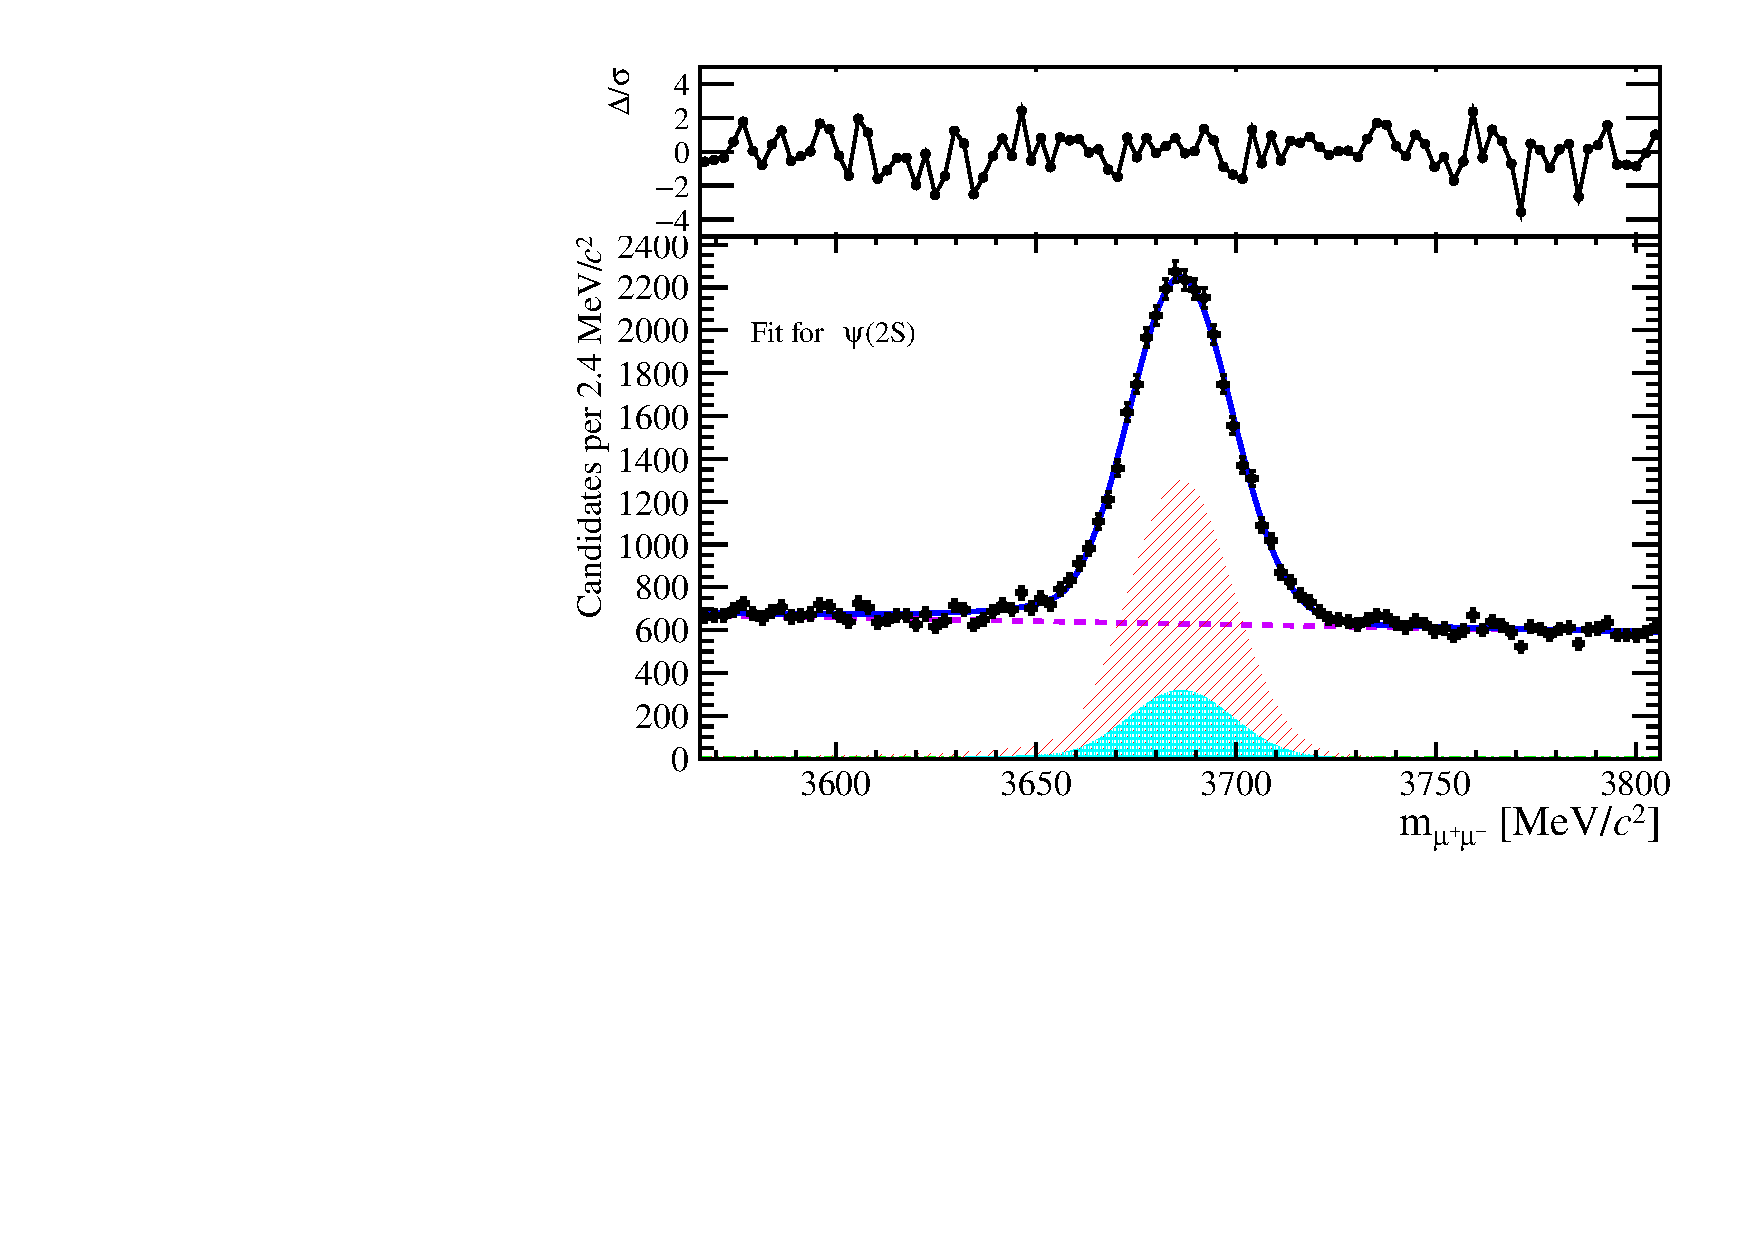
\includegraphics[width=0.49\linewidth]{pdf/Psi2S/drawmass/n2y1pt2.pdf}
   \end{center}
   \caption{
     Projection in $t_z$ and mass spectrum of $t_z$-mass fit for PVNTRACKS from 20 to 40, y from 2 to 2.8, and pt from 2$\gevc$ to 4 $\gevc$. The left is that of $\jpsi$ and the right is of $\psitwos$.
     }
   \label{fig:2Dtz}
 \end{figure}
%%%%%%%%%%%%%%%%%%%%%%%%%%%%%%%%%%%%%%%%%%%%%%%%%%%%%%%%%%%


\section{Efficiency determination}\label{sec:efficiency}
\def\effTot{\ensuremath{\epsilon_{\mathrm{tot}}}\xspace}
\def\effAcc{\ensuremath{\epsilon_{\mathrm{acc}}}\xspace}
\def\effReco{\ensuremath{\epsilon_{\mathrm{Reco\&Sel}}}\xspace}
\def\effID{\ensuremath{\epsilon_{\mathrm{MuonID}}}\xspace}
\def\effTrigger{\ensuremath{\epsilon_{\mathrm{Trigger}}}\xspace}
The total efficiency \effTot is determined independently in each kinetic bin and multiplicity 
bin. The expression is as follows,
\begin{equation}
    \effTot = \effAcc \times \effReco \times \effID \times \effTrigger.
\end{equation}
The Monte Carlo samples for both prompt and non-prompt signals of \jpsi and \psitwos are divided according to the multiplicity binning schemes in Sec.~\ref{Ratio of Cross-Section Determination}. 
For different multiplicity regions based on division upon different multiplicity variables, efficiencies are calculated in the same way as follows, which is calculated in the same binning scheme for kinematic variables \pt and $y$. 
The truth-matching fail rates for both \jpsi and \psitwos are around $0.4\%$, which is negligible compared to the statistical 
and systematic uncertainties after division to get the ratio. And in the simulated sample, the efficiency of prompt components 
and components from $b$-hadron decay is calculated separately. Since we have already separated 
the data and MC in a multiplicity bin, the bin width of \pt and $y$ is not significantly small 
that the efficiency can be treated as constant in a certain kinetic bin, hence, all the efficiencies 
are corrected by reweighting the distribution of \pt-$y$ spectrum of MC to that of s-weighted data 
which contains only signal by sPlot method~\cite{Pivk:2004ty}. Also, the effect due to the difference in the distribution of 
multiplicity is corrected by reweighting the distribution of multiplicity variables of MC to that of 
s-weighted data which contains only signal. Since there are differences in the distribution of \pt-$y$ spectrum and multiplicity variables for prompt and non-prompt signals, 
before calculating efficiencies, we reweight the \pt-$y$ and multiplicity distributions separately for prompt and non-prompt signals, as shown in Figs~\ref{reweight}.
\begin{figure}[H]
    \begin{center}
      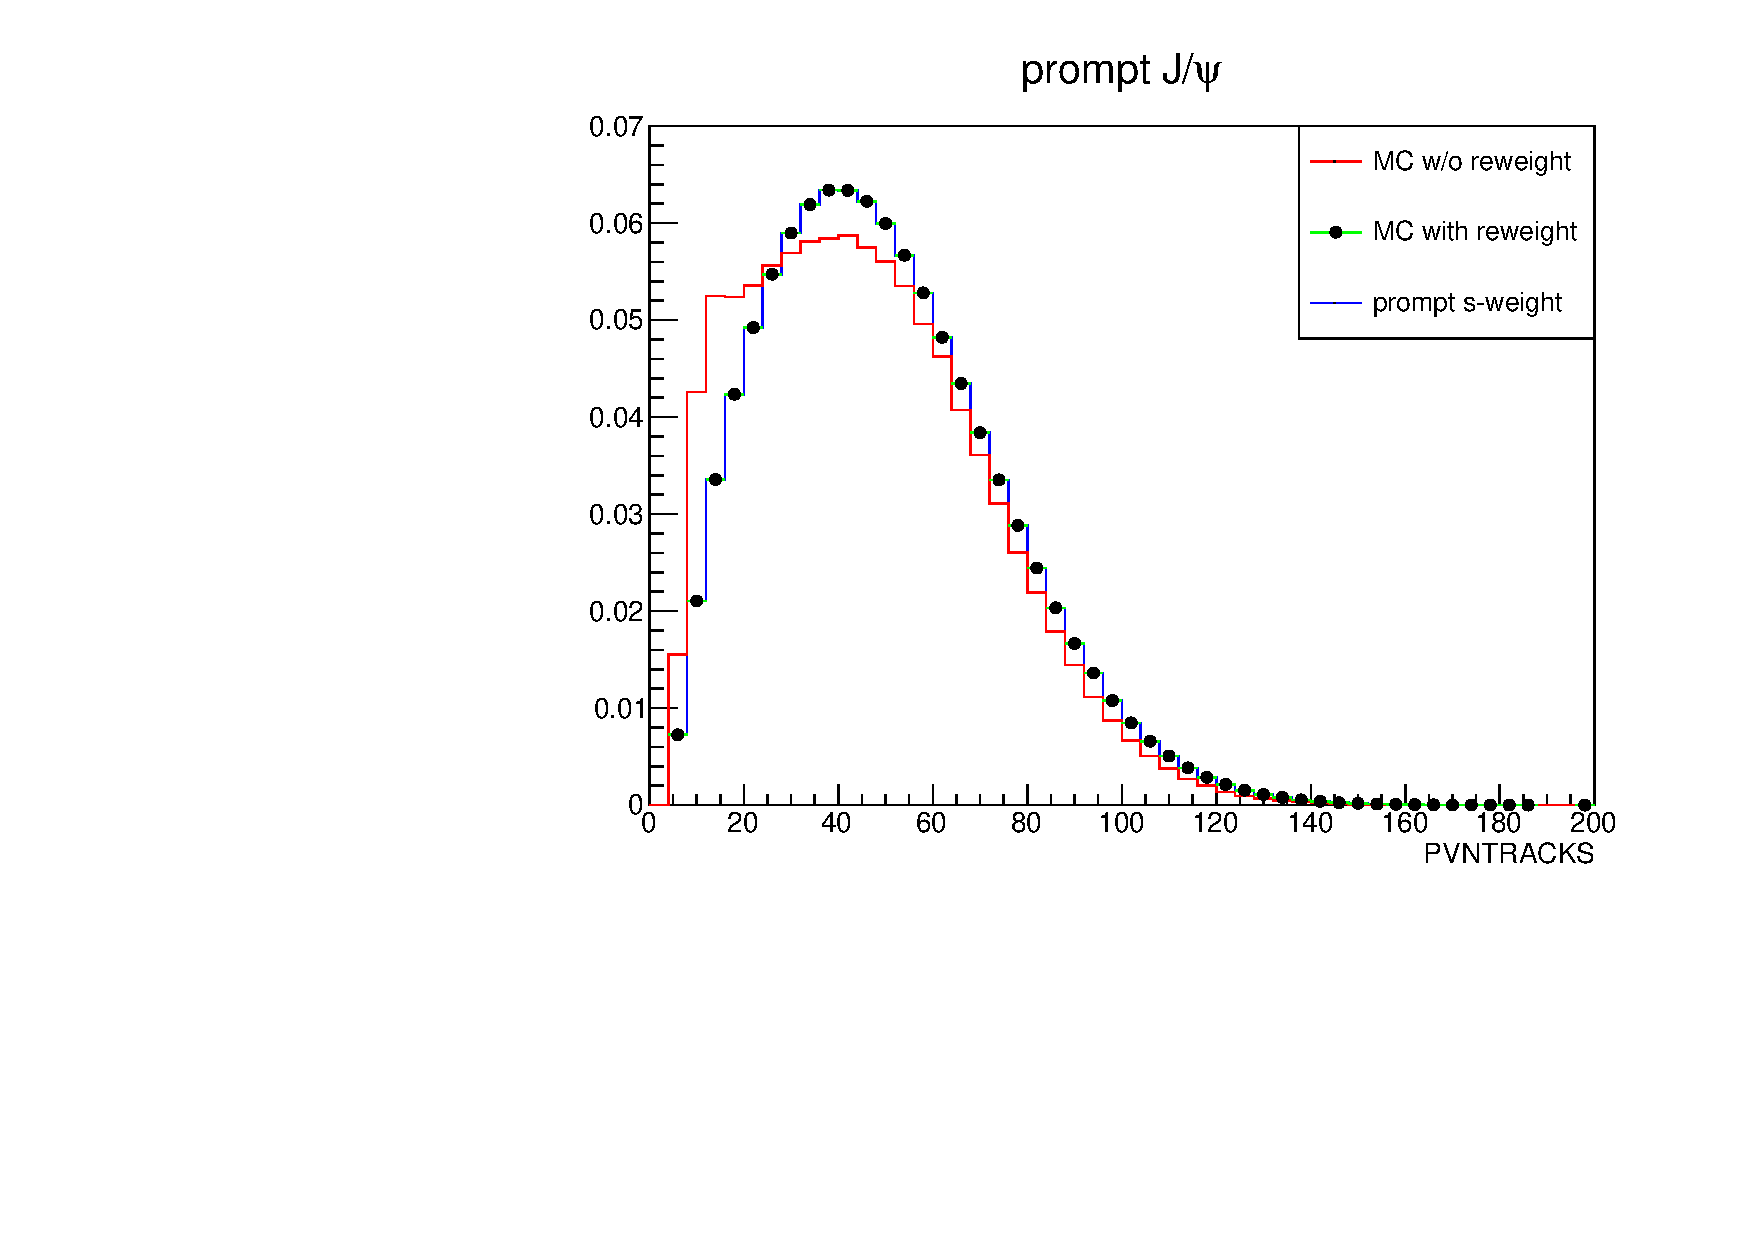
\includegraphics[width=0.25\linewidth]{pdf/Jpsi/reweight/np.pdf}
      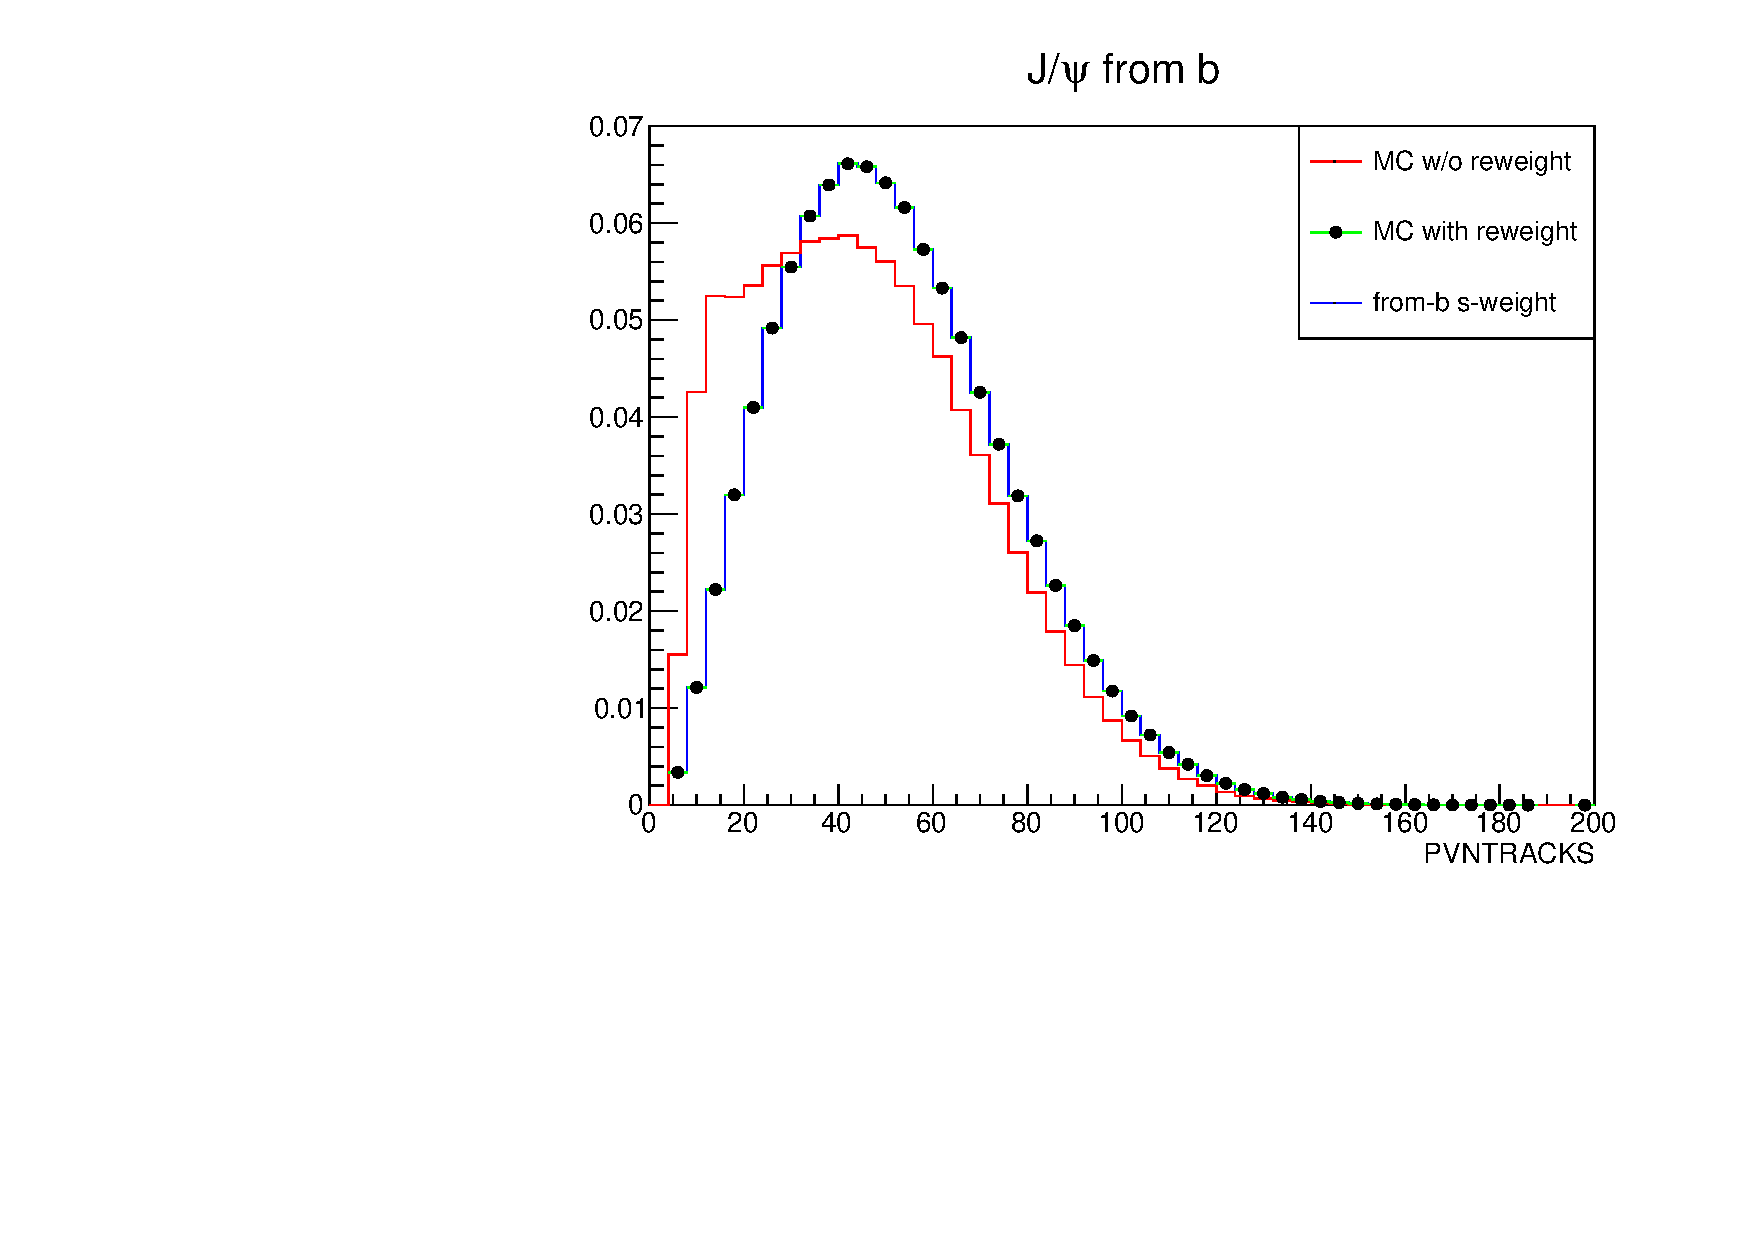
\includegraphics[width=0.25\linewidth]{pdf/Jpsi/reweight/nb.pdf}
      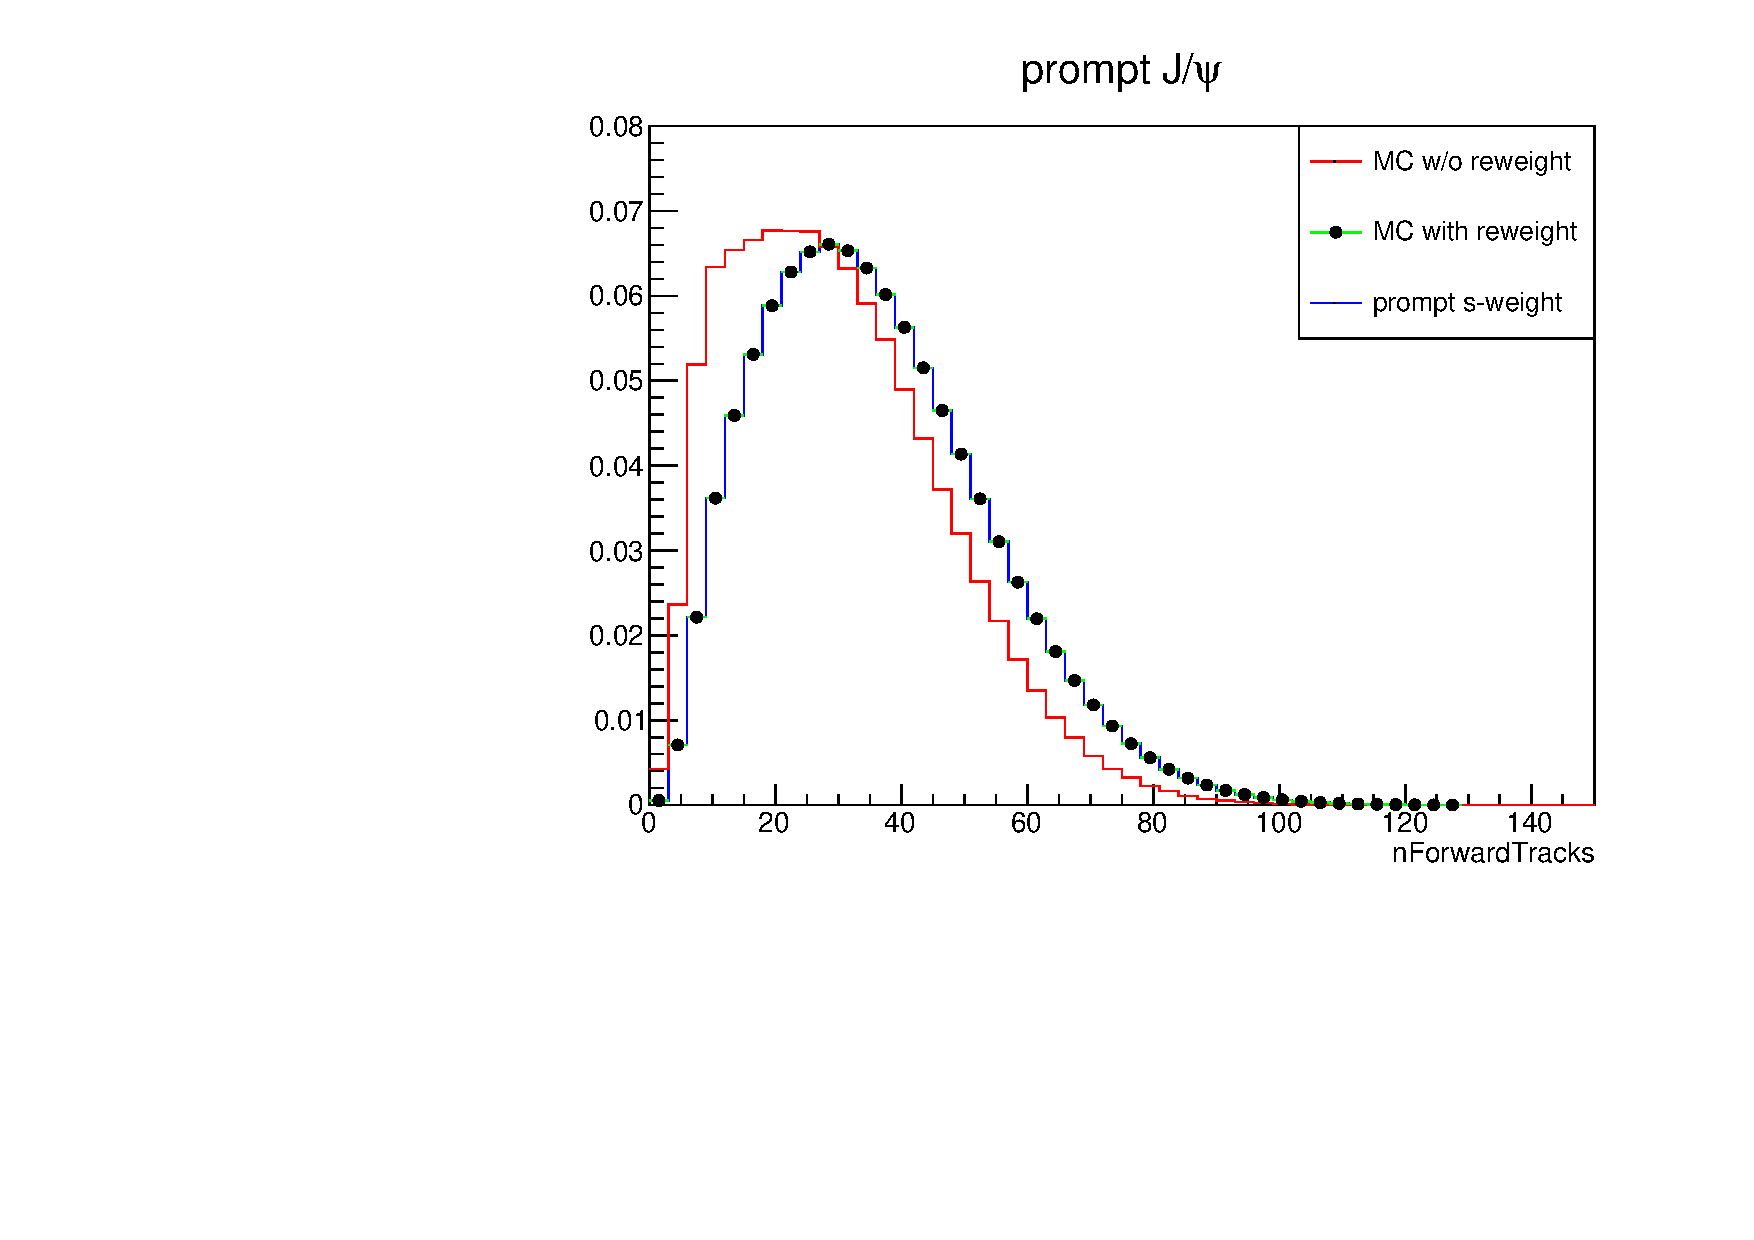
\includegraphics[width=0.25\linewidth]{pdf/Jpsi/reweight/npF.pdf}
      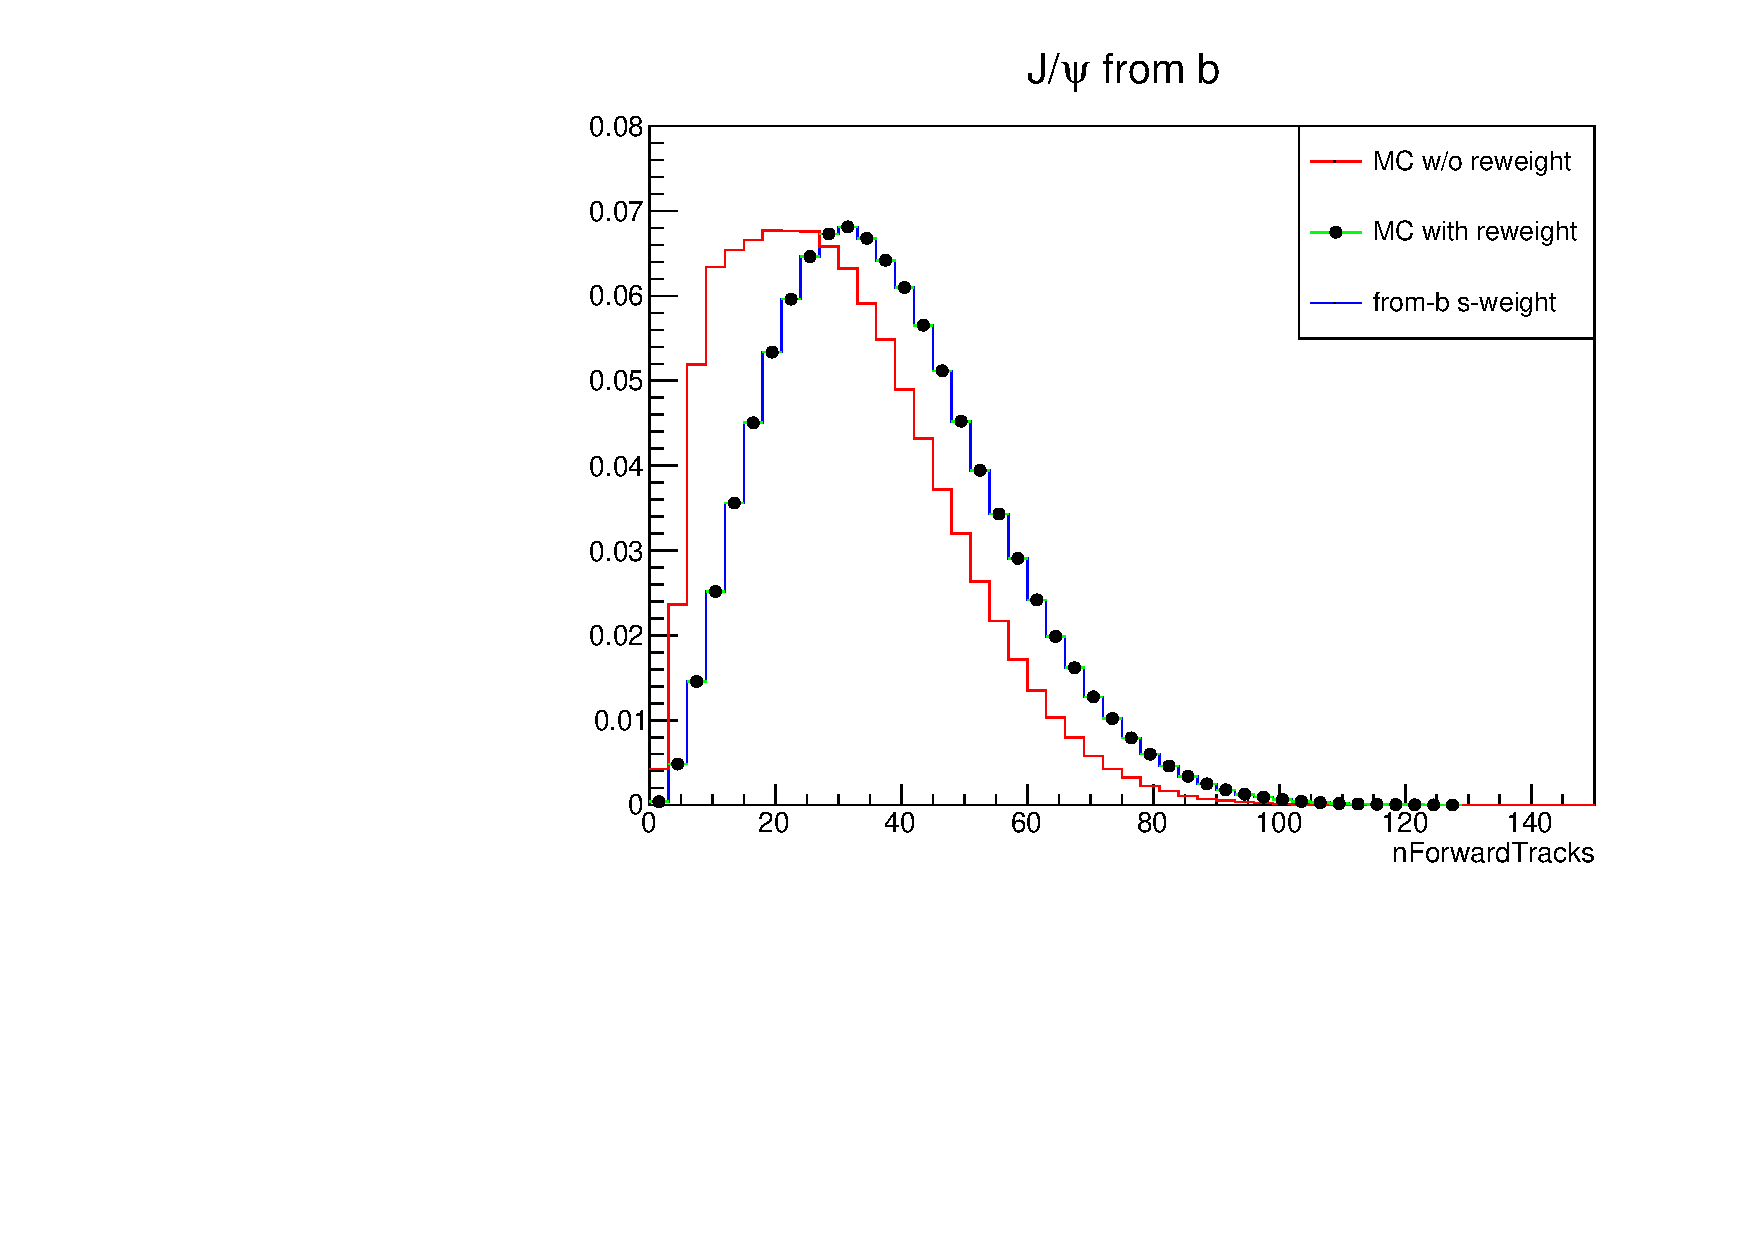
\includegraphics[width=0.25\linewidth]{pdf/Jpsi/reweight/nbF.pdf}
      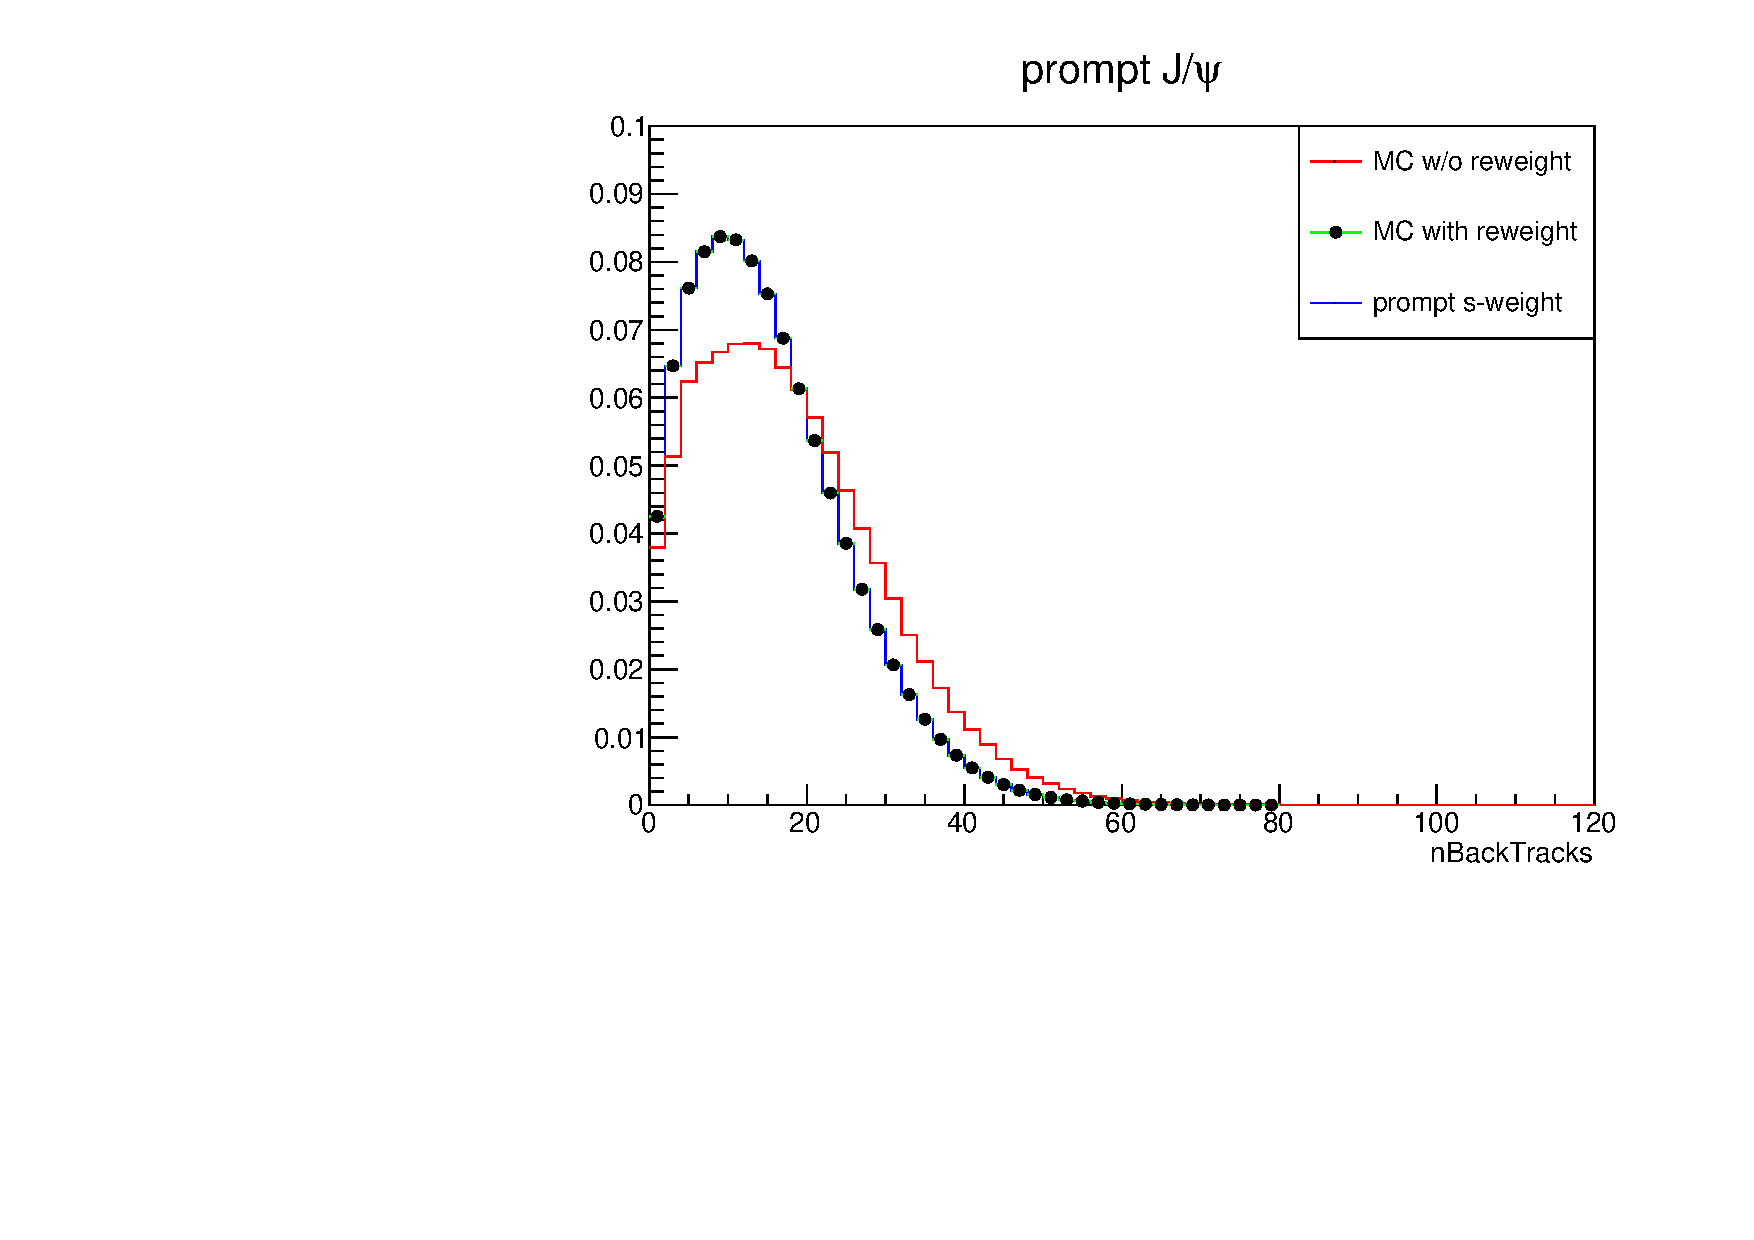
\includegraphics[width=0.25\linewidth]{pdf/Jpsi/reweight/npB.pdf}
      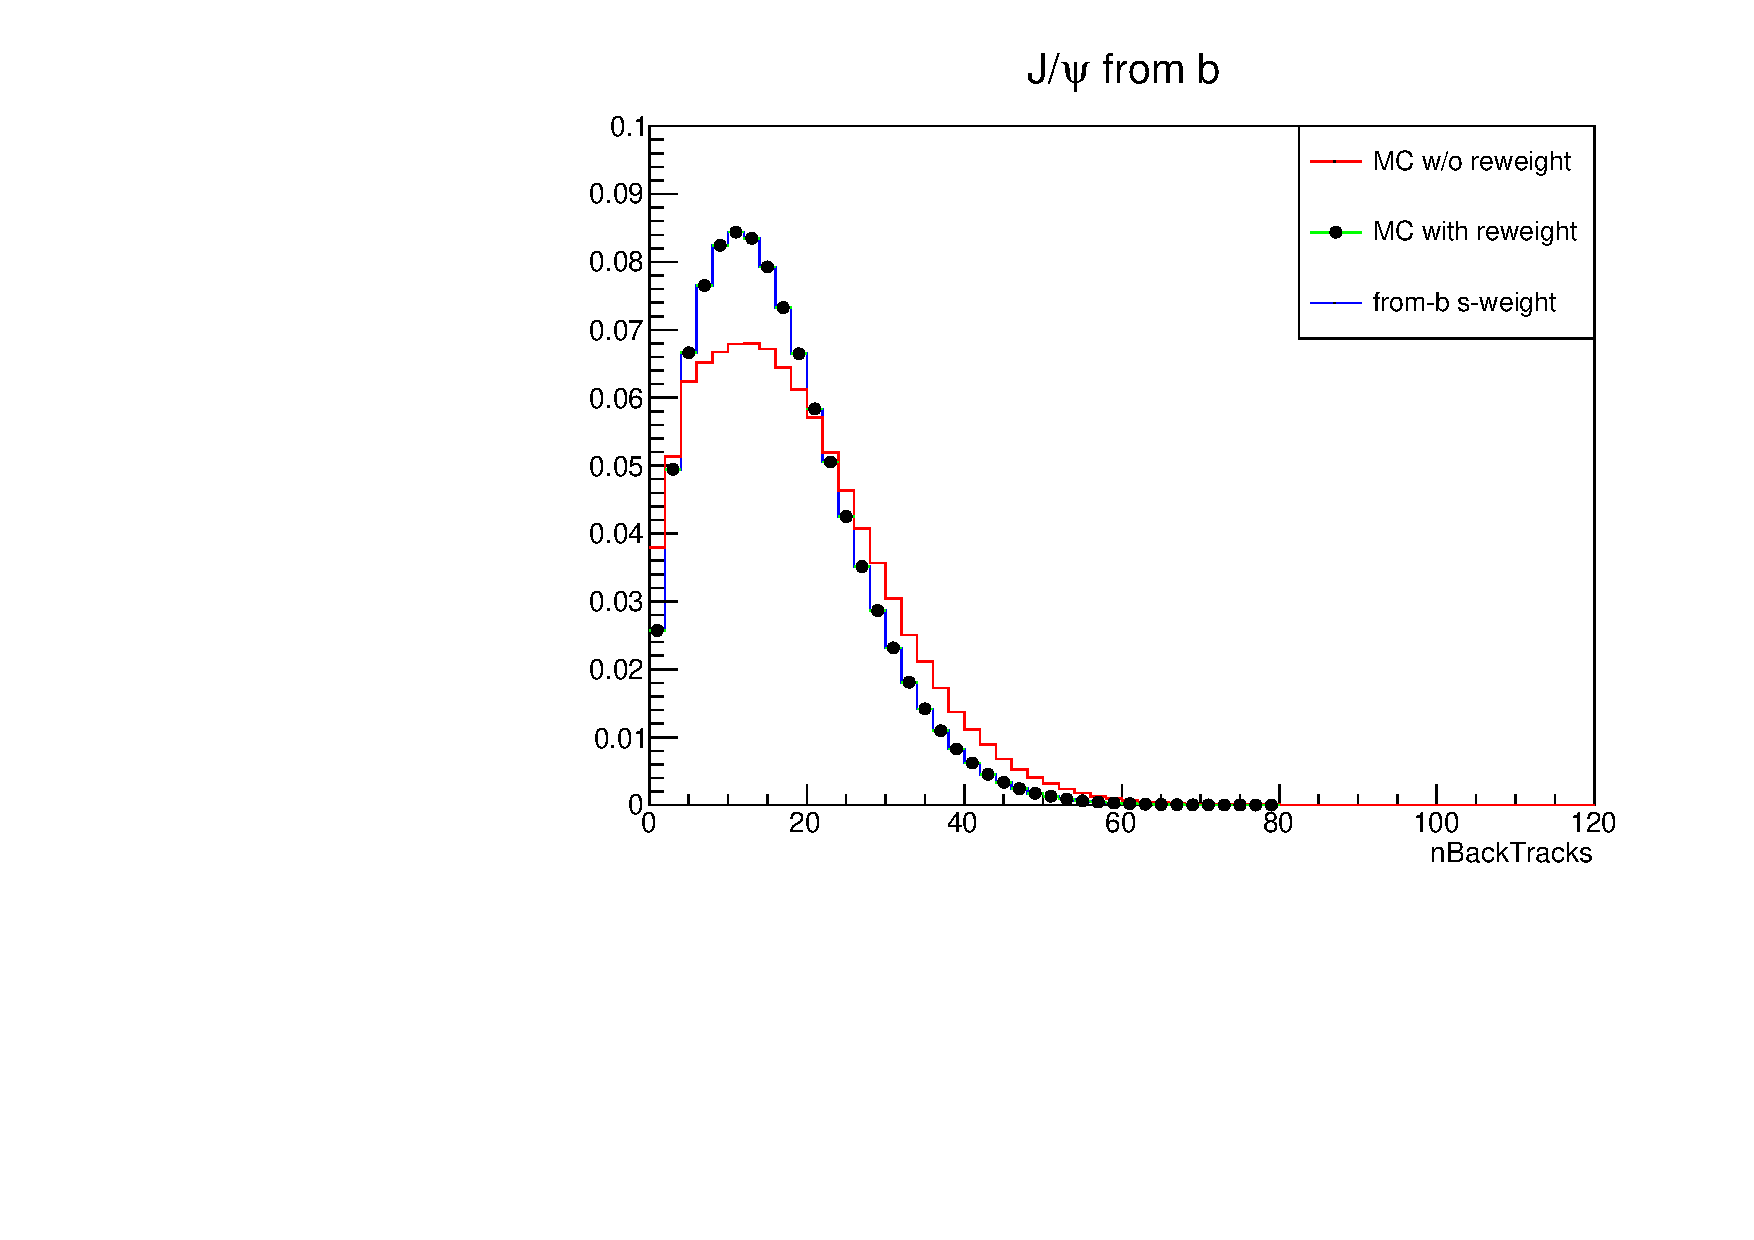
\includegraphics[width=0.25\linewidth]{pdf/Jpsi/reweight/nbB.pdf}
      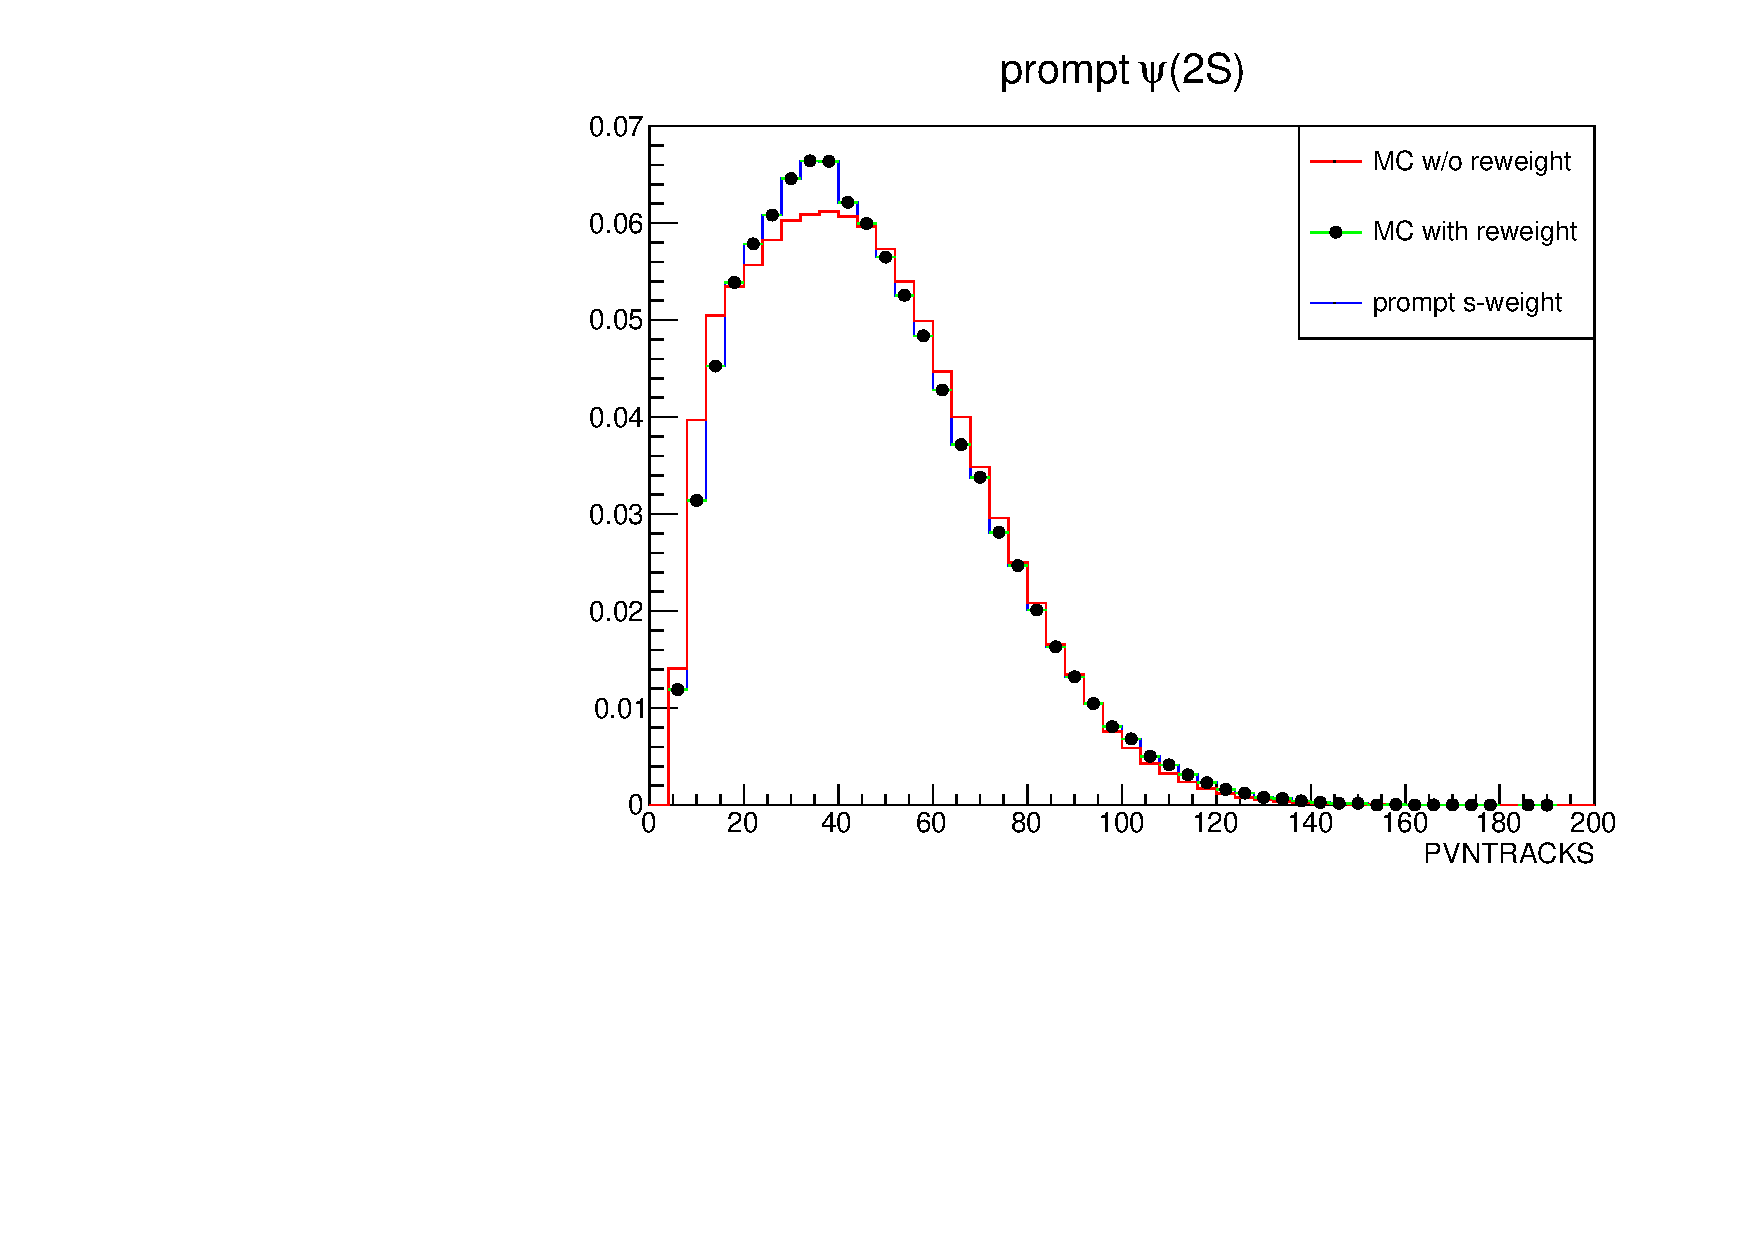
\includegraphics[width=0.25\linewidth]{pdf/Psi2S/reweight/np.pdf}
      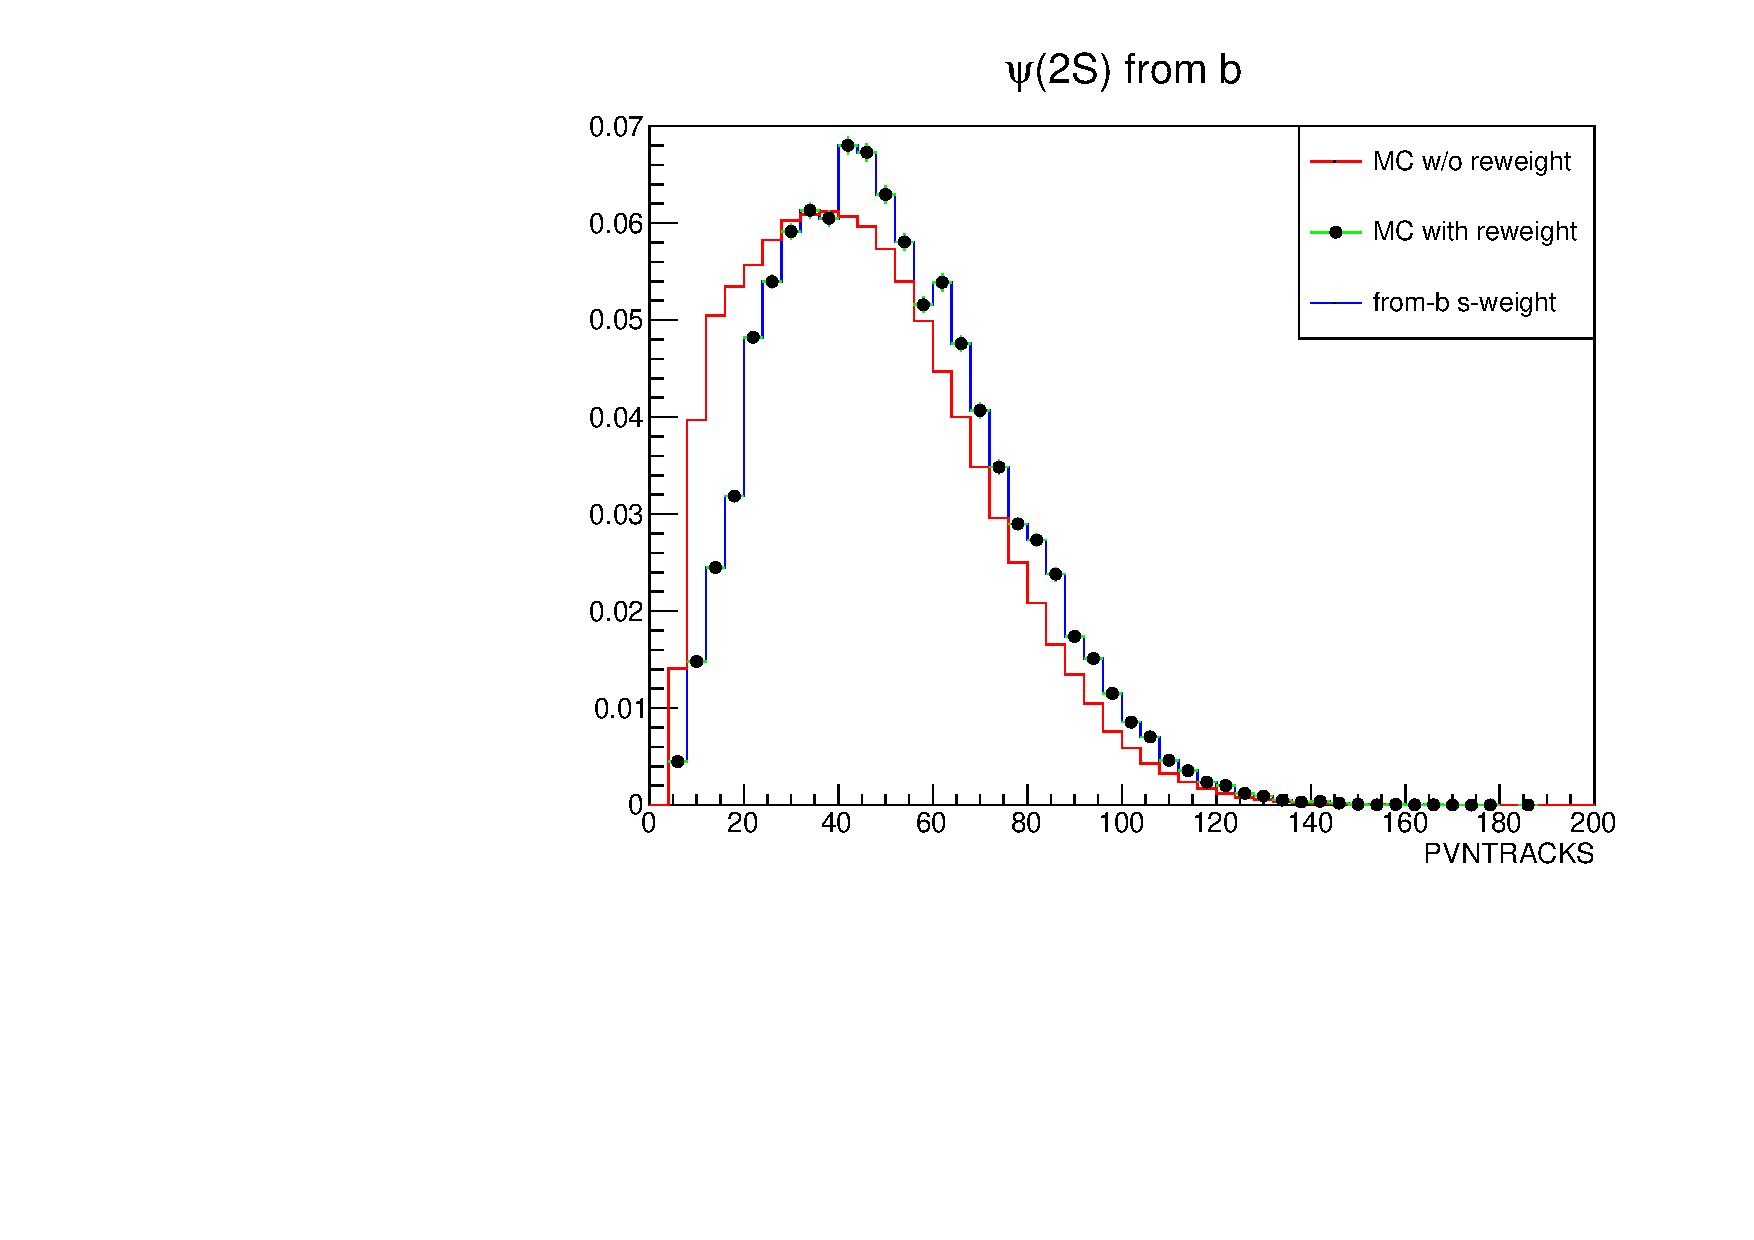
\includegraphics[width=0.25\linewidth]{pdf/Psi2S/reweight/nb.pdf}
      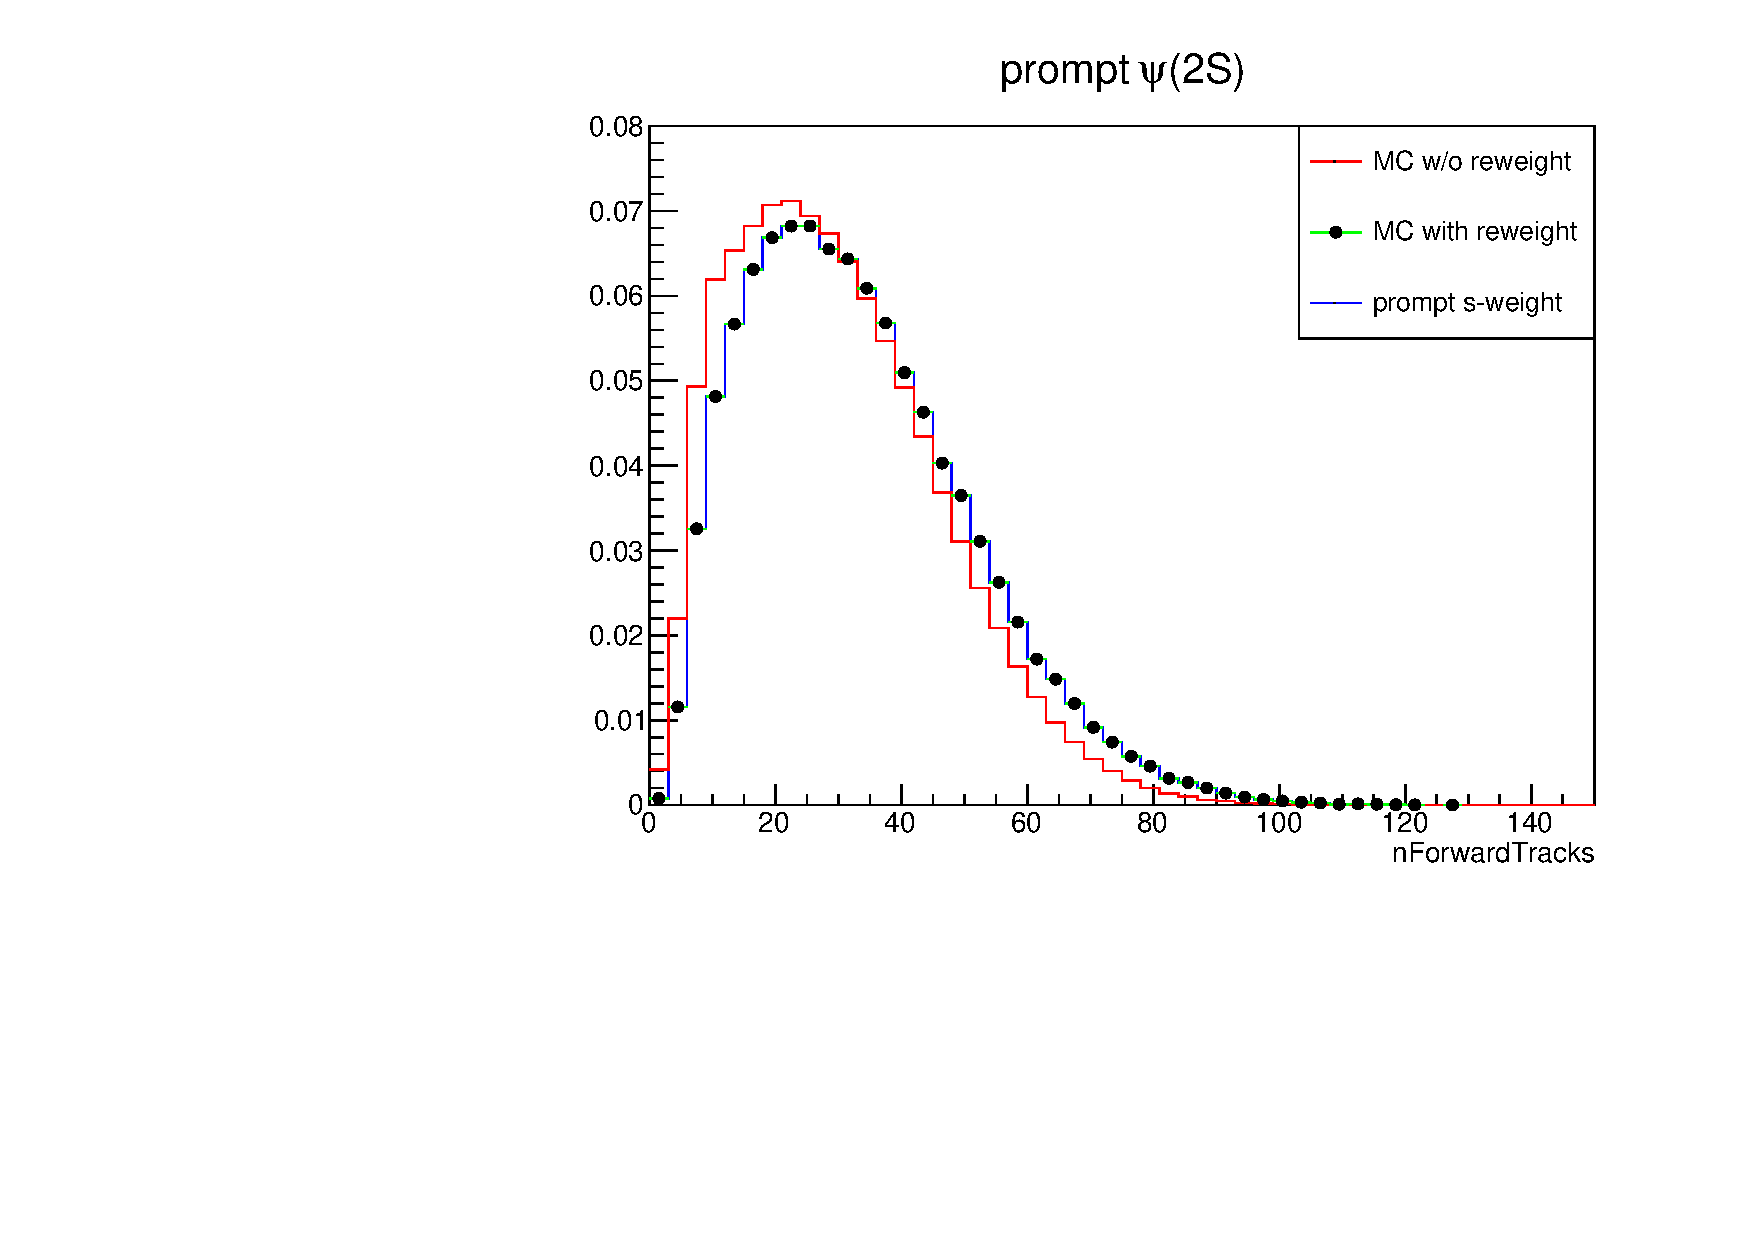
\includegraphics[width=0.25\linewidth]{pdf/Psi2S/reweight/npF.pdf}
      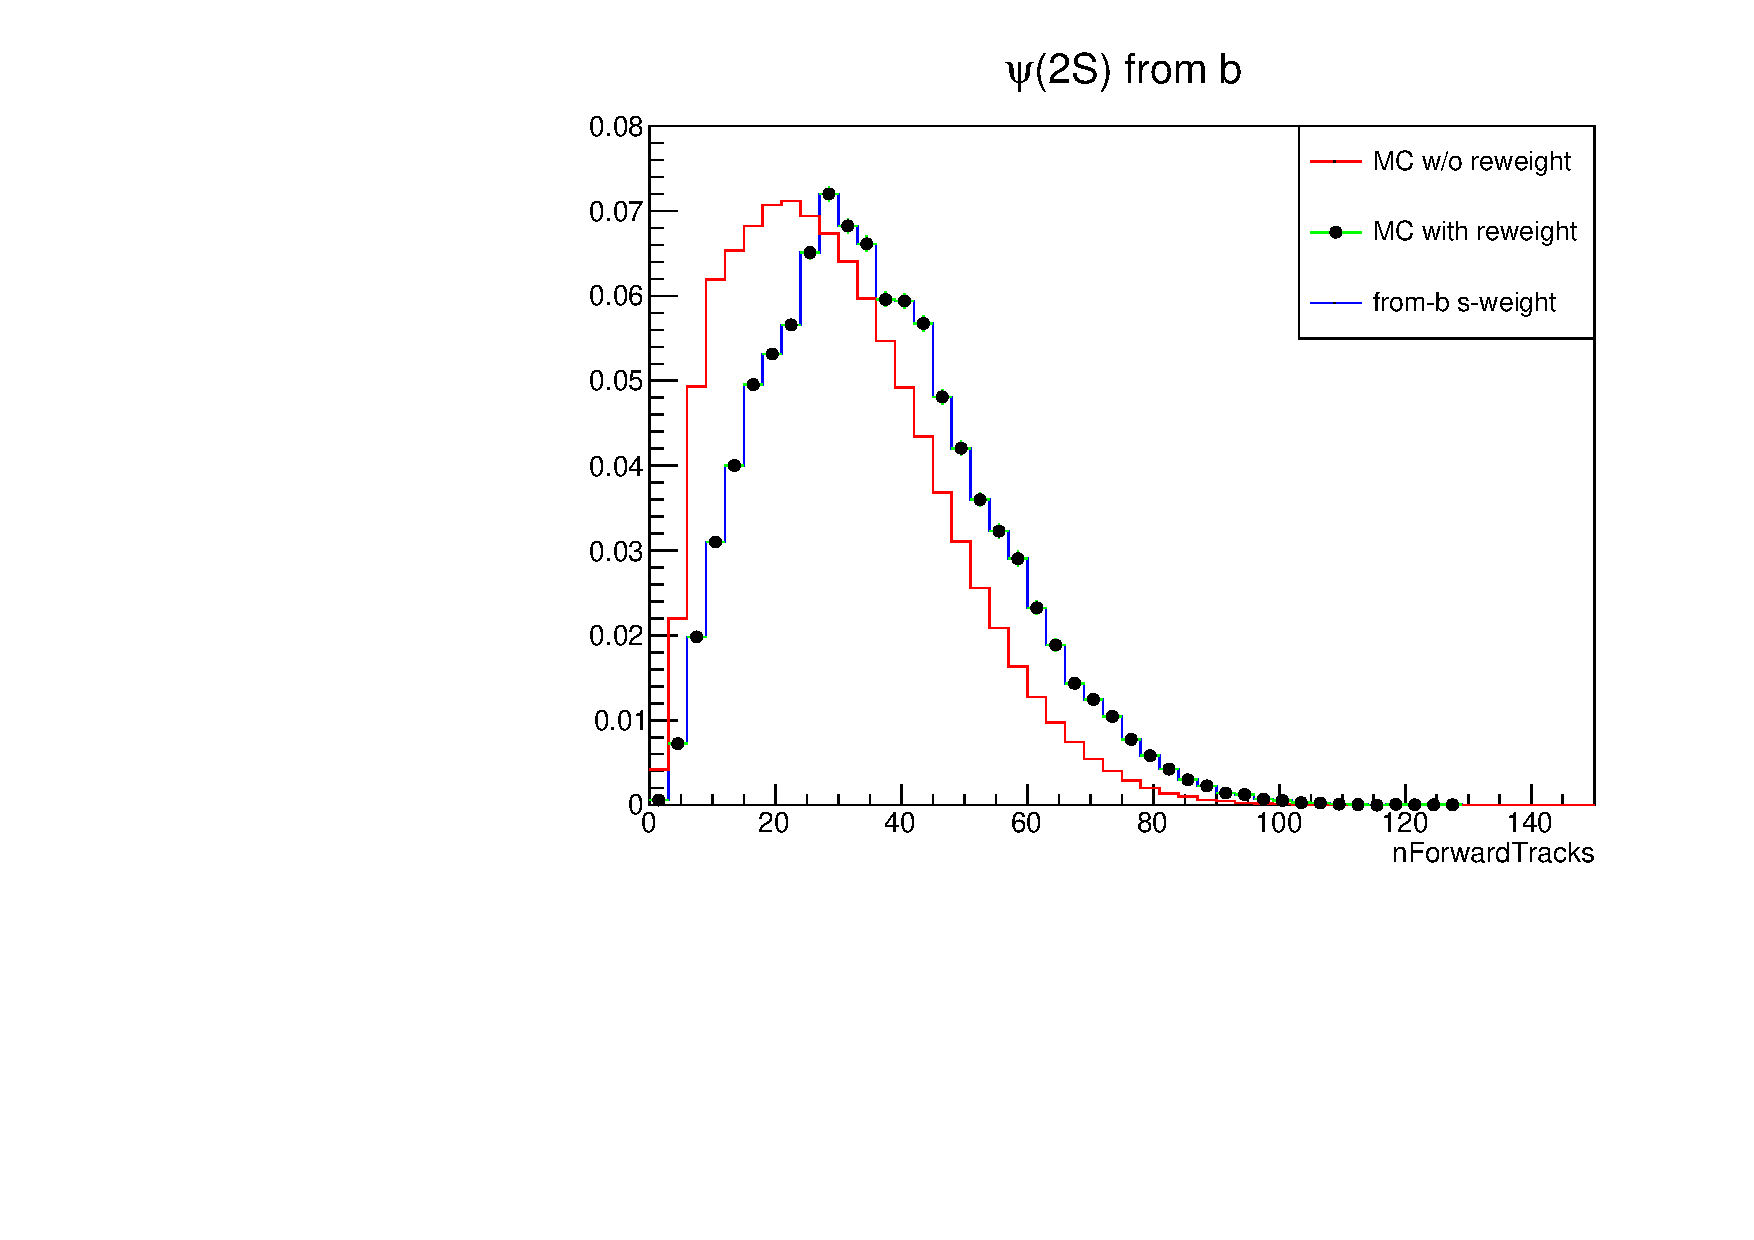
\includegraphics[width=0.25\linewidth]{pdf/Psi2S/reweight/nbF.pdf}
      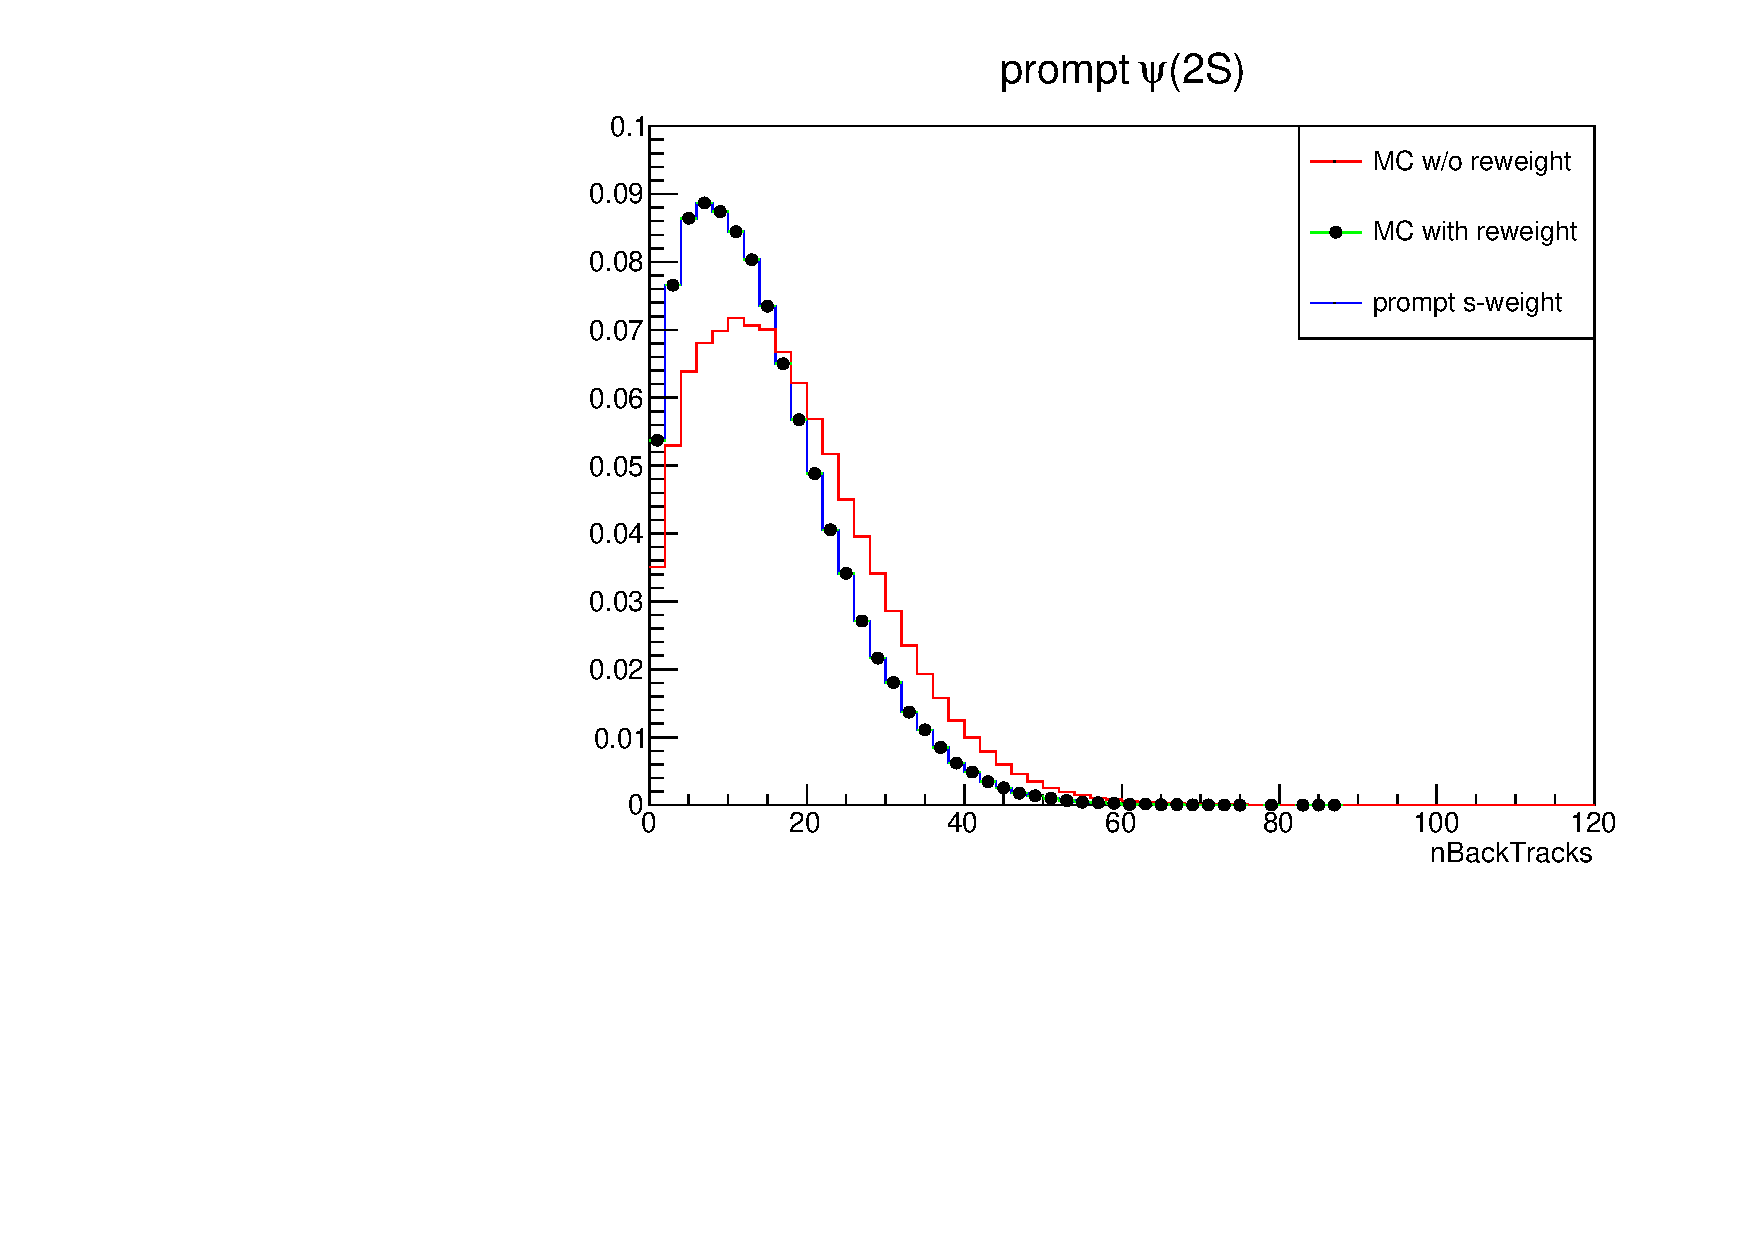
\includegraphics[width=0.25\linewidth]{pdf/Psi2S/reweight/npB.pdf}
      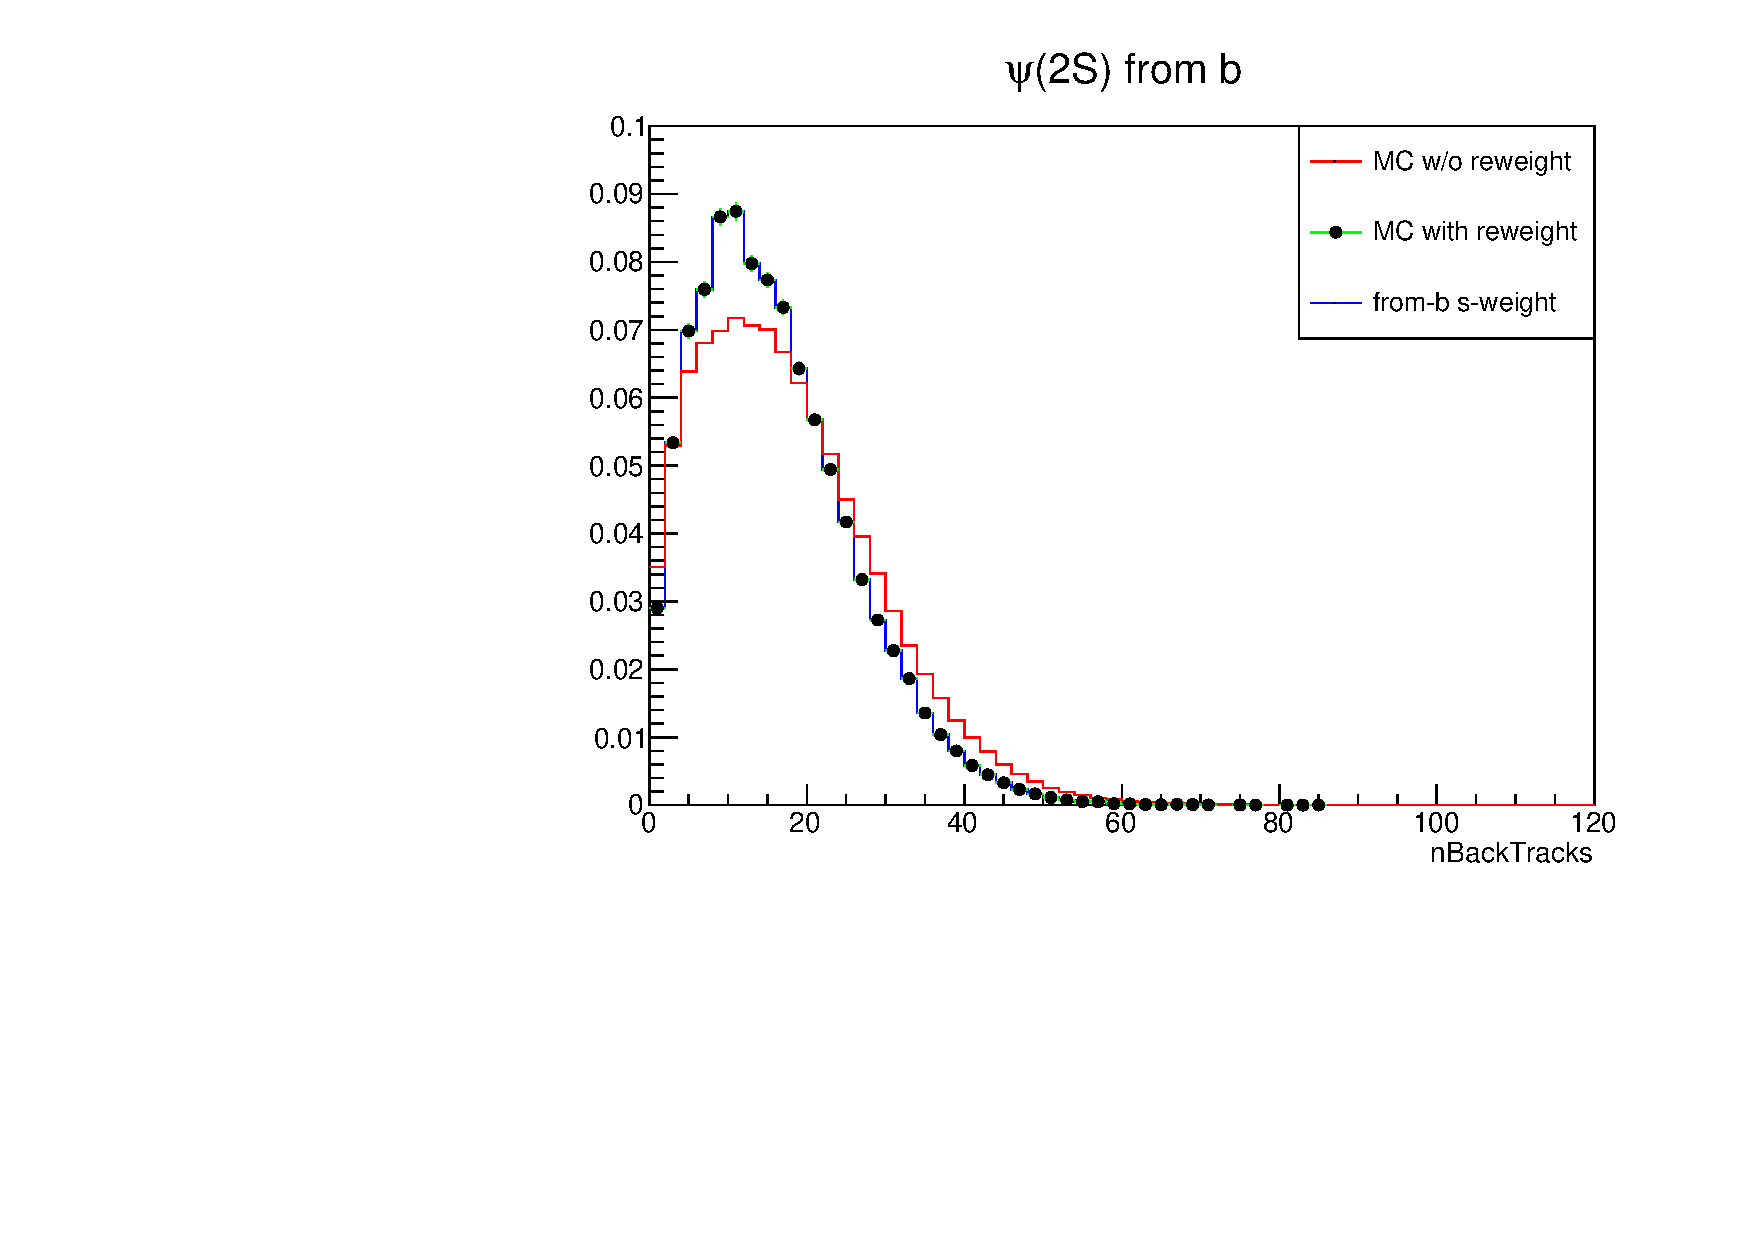
\includegraphics[width=0.25\linewidth]{pdf/Psi2S/reweight/nbB.pdf}
    \end{center}
    \caption{
      Reweight the multiplicity distribution to match MC to s-weighted data, the first two rows are reweight of \jpsi and the rest two rows are of $\psitwos$.}
    \label{reweight}
\end{figure}
For \jpsi \pt-$y$ reweight, the results cut in each $y$ region for $\jpsi$ is shown in Figs~\ref{JreweightPTY}. And the result for \psitwos is shown in Figs~\ref{PreweightPTY}.
\begin{figure}[h]
    \begin{center}
      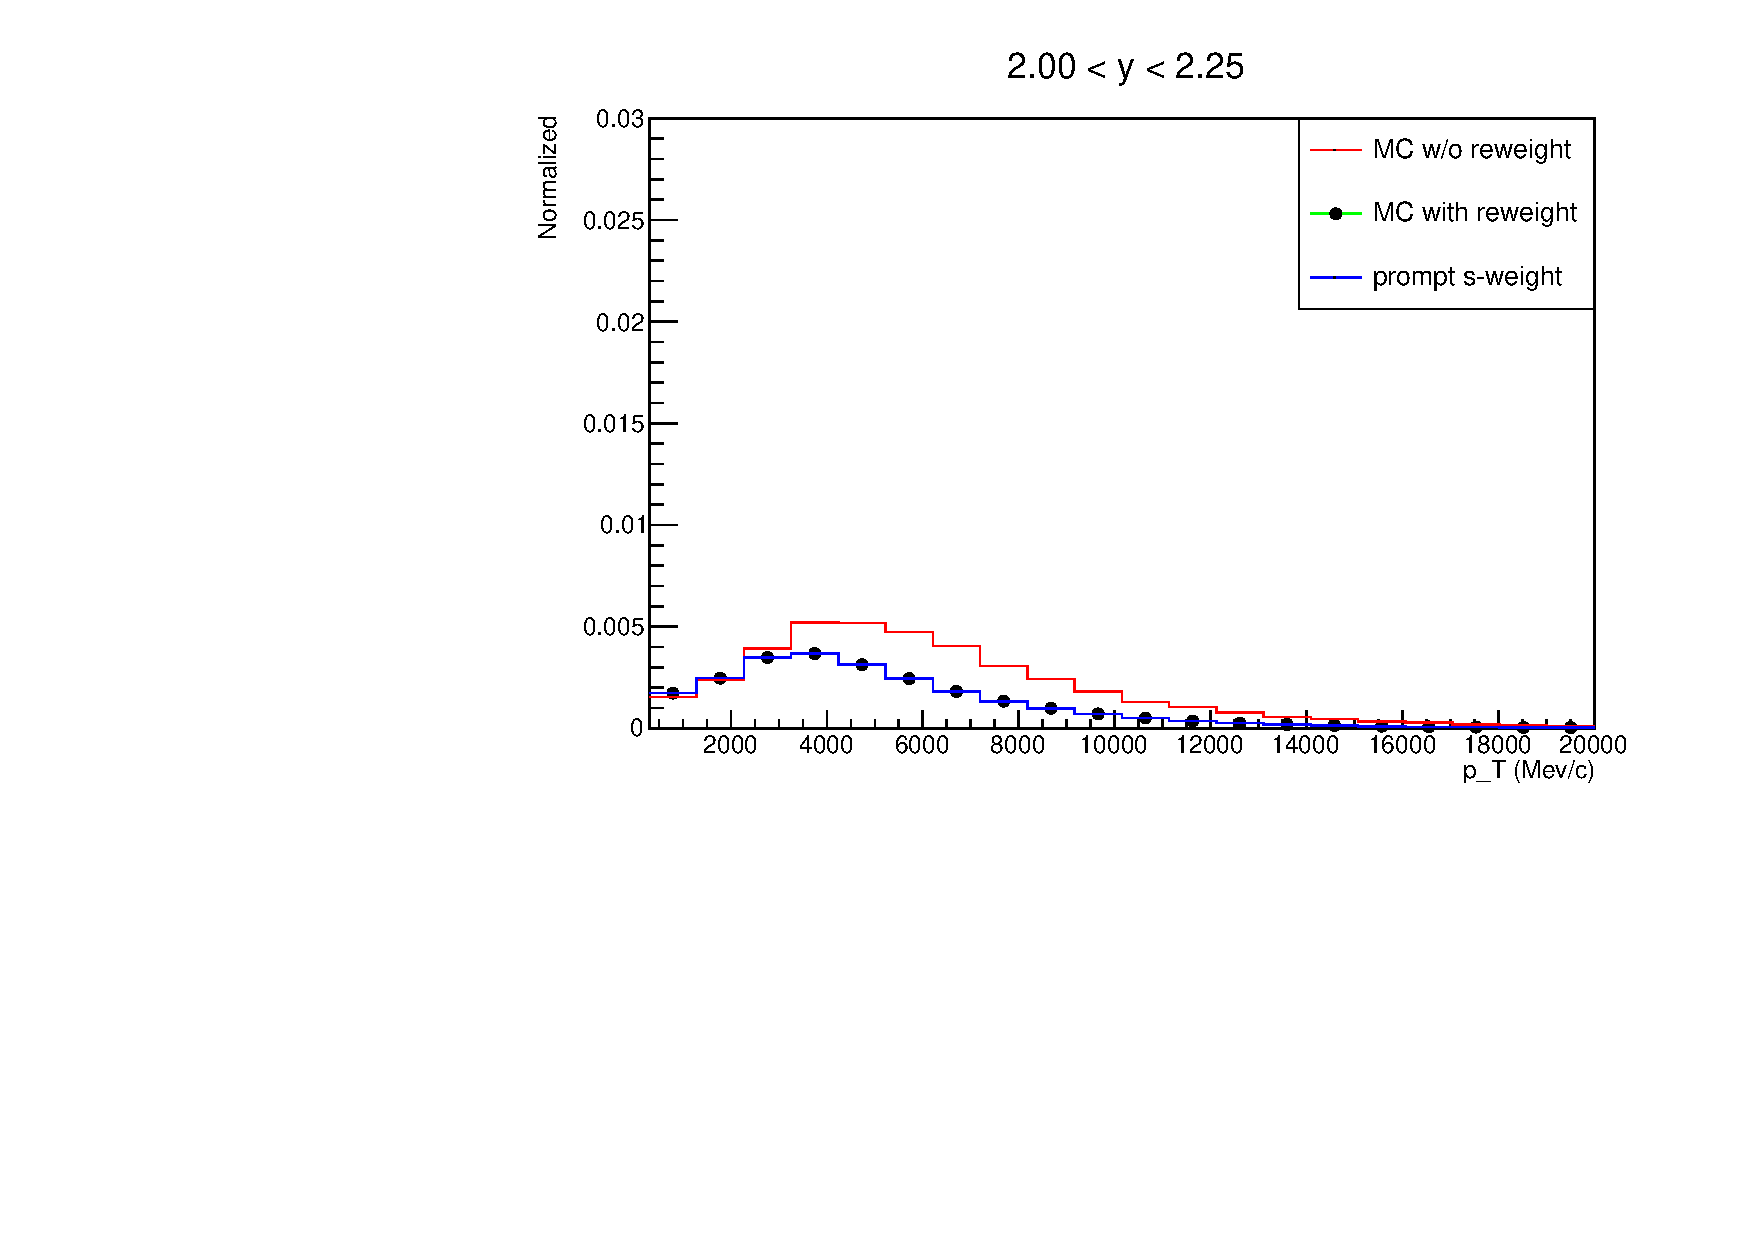
\includegraphics[width=0.19\linewidth]{pdf/Jpsi/reweight/Yp1.pdf}
      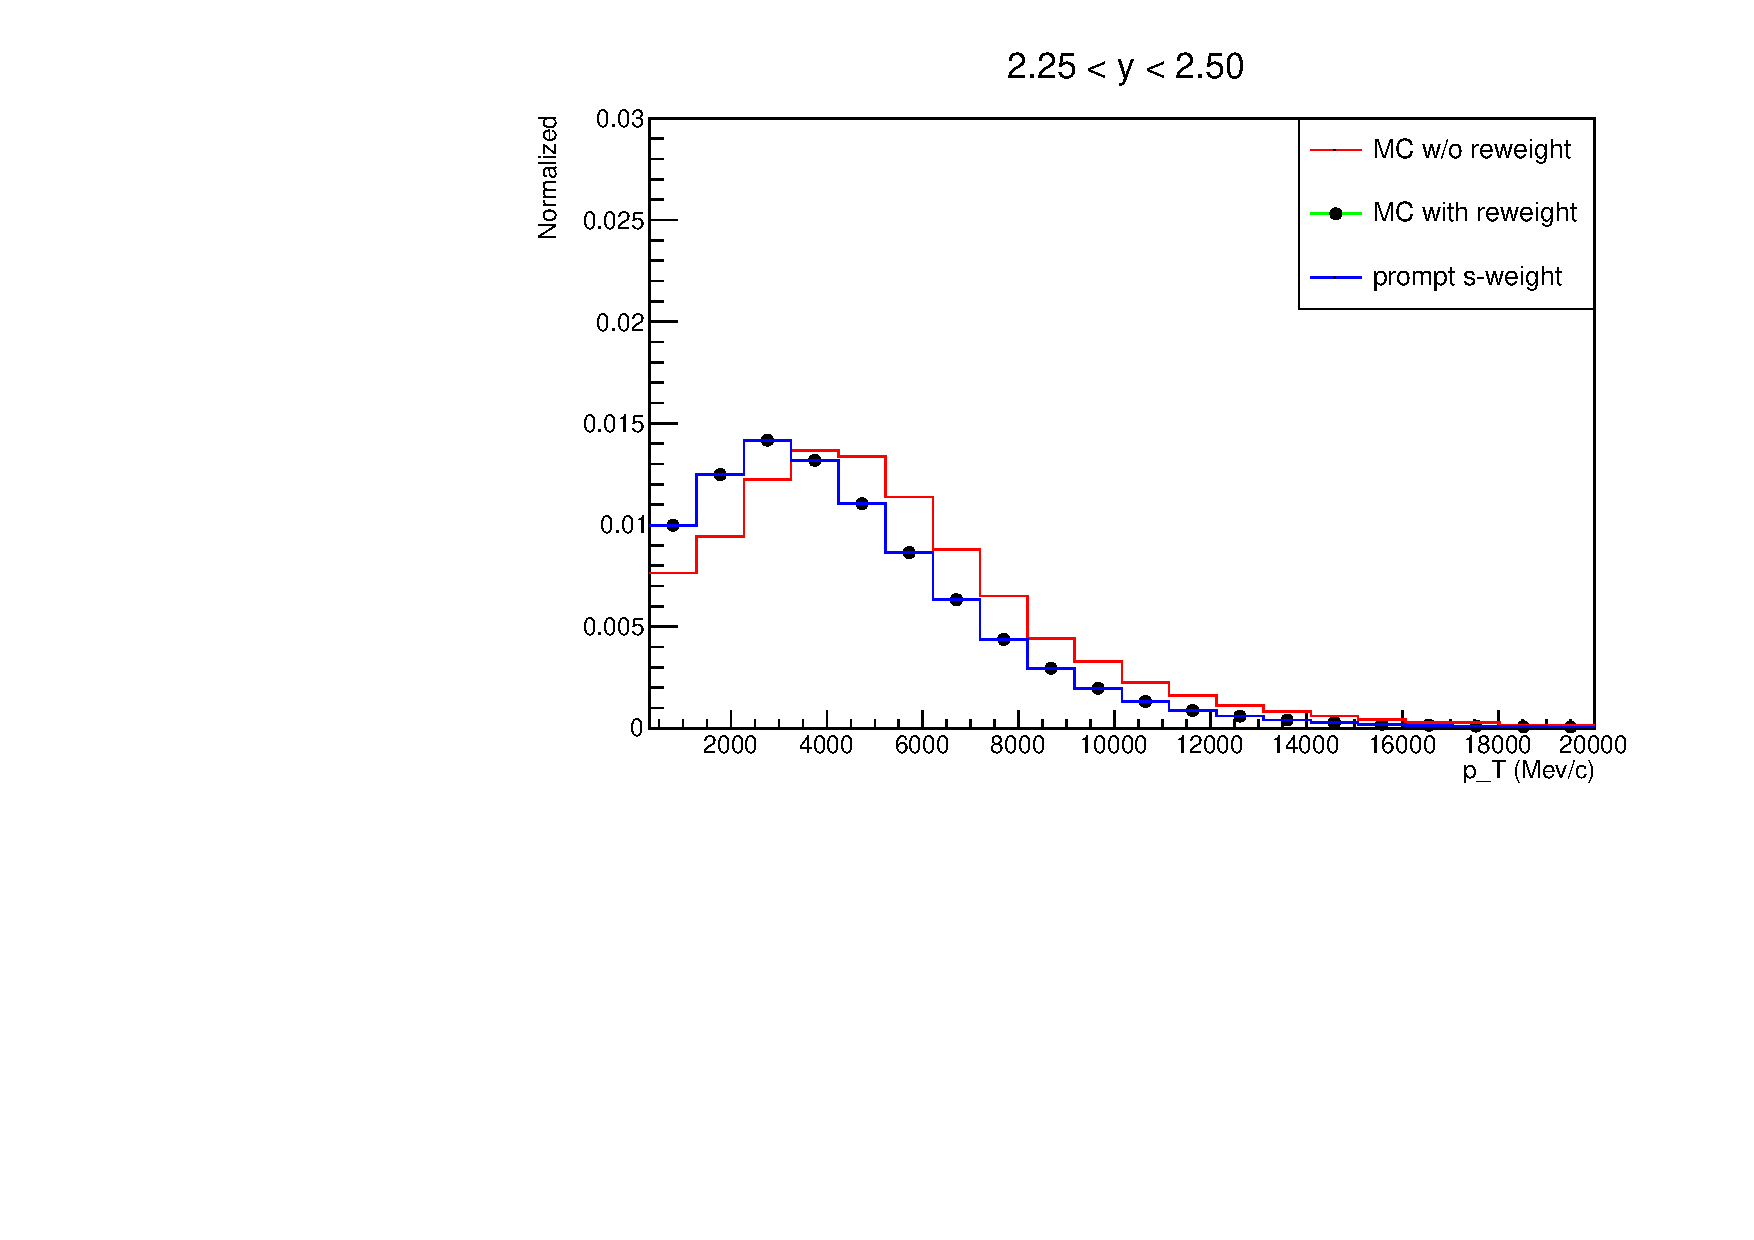
\includegraphics[width=0.19\linewidth]{pdf/Jpsi/reweight/Yp2.pdf} 
      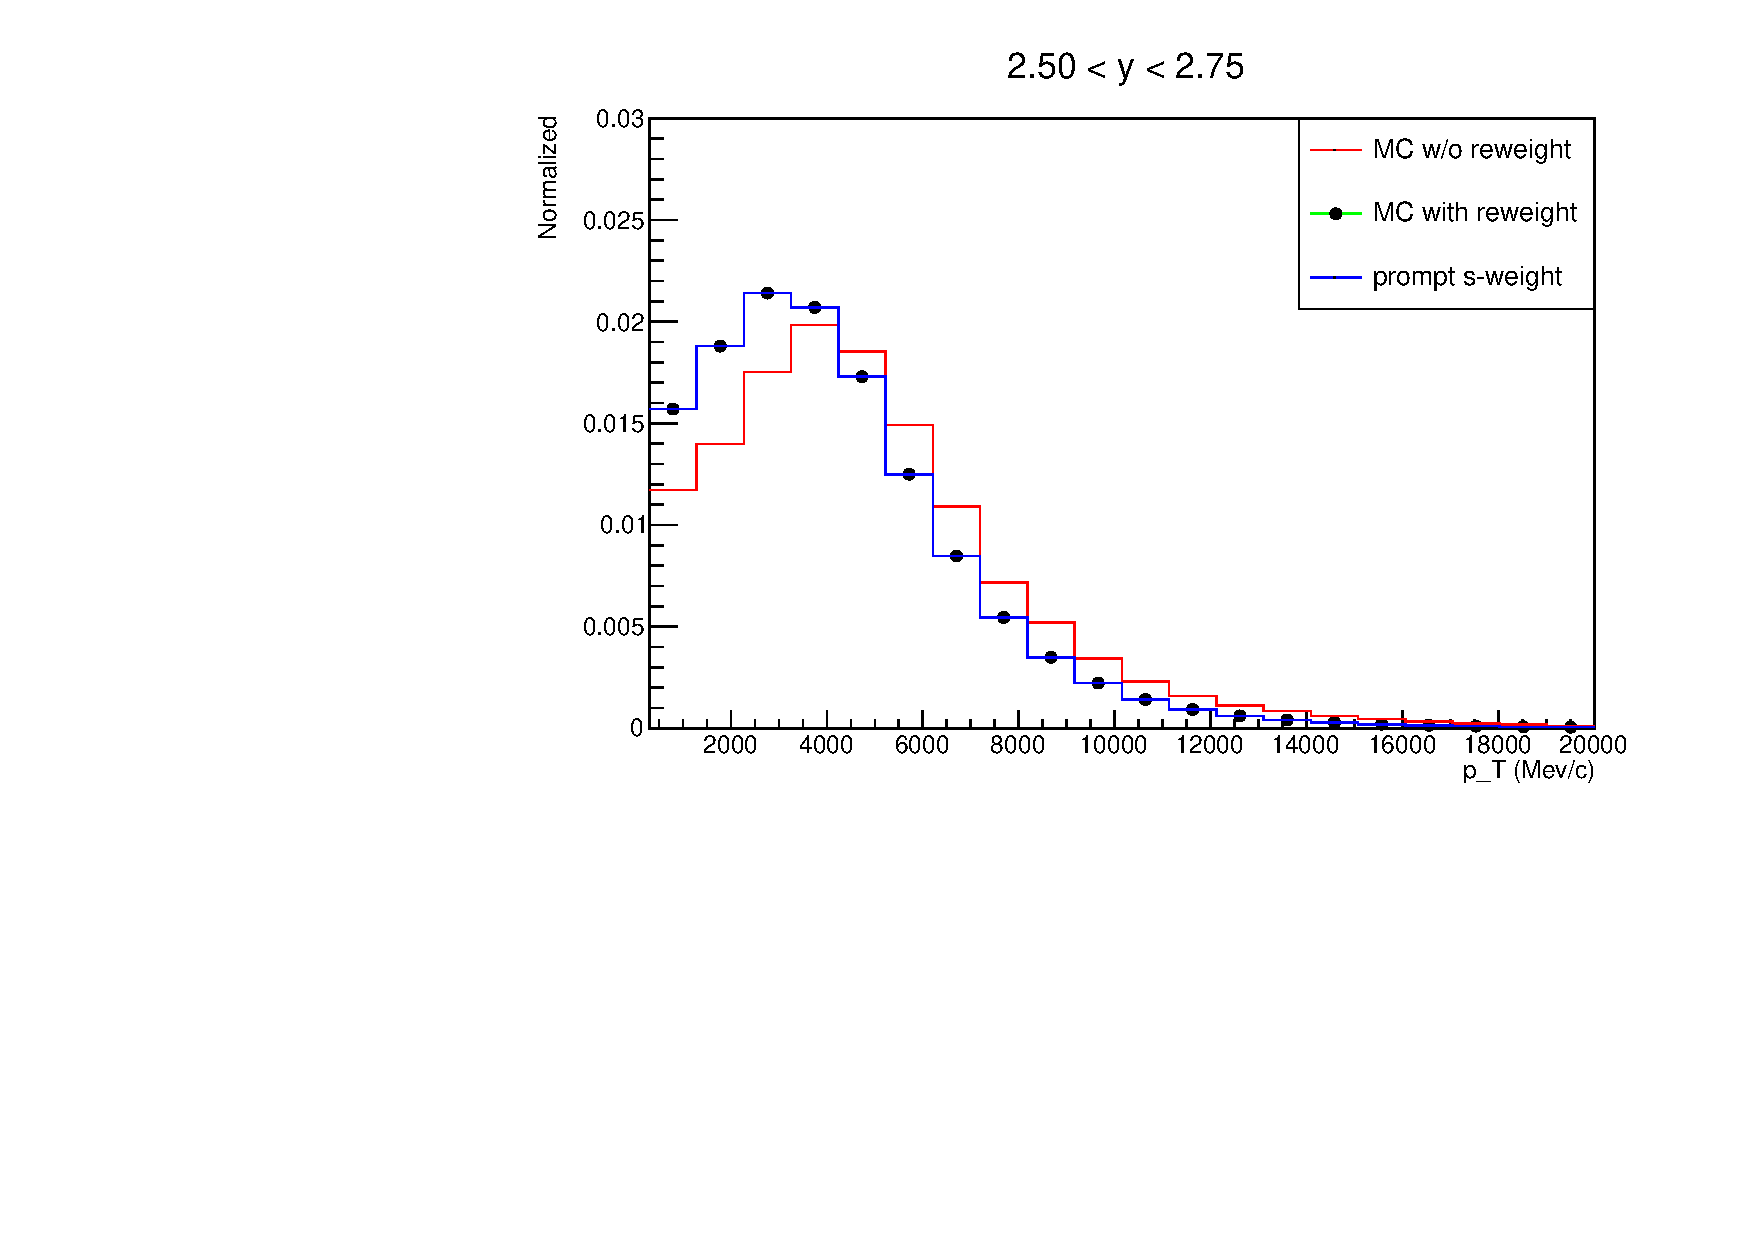
\includegraphics[width=0.19\linewidth]{pdf/Jpsi/reweight/Yp3.pdf}
      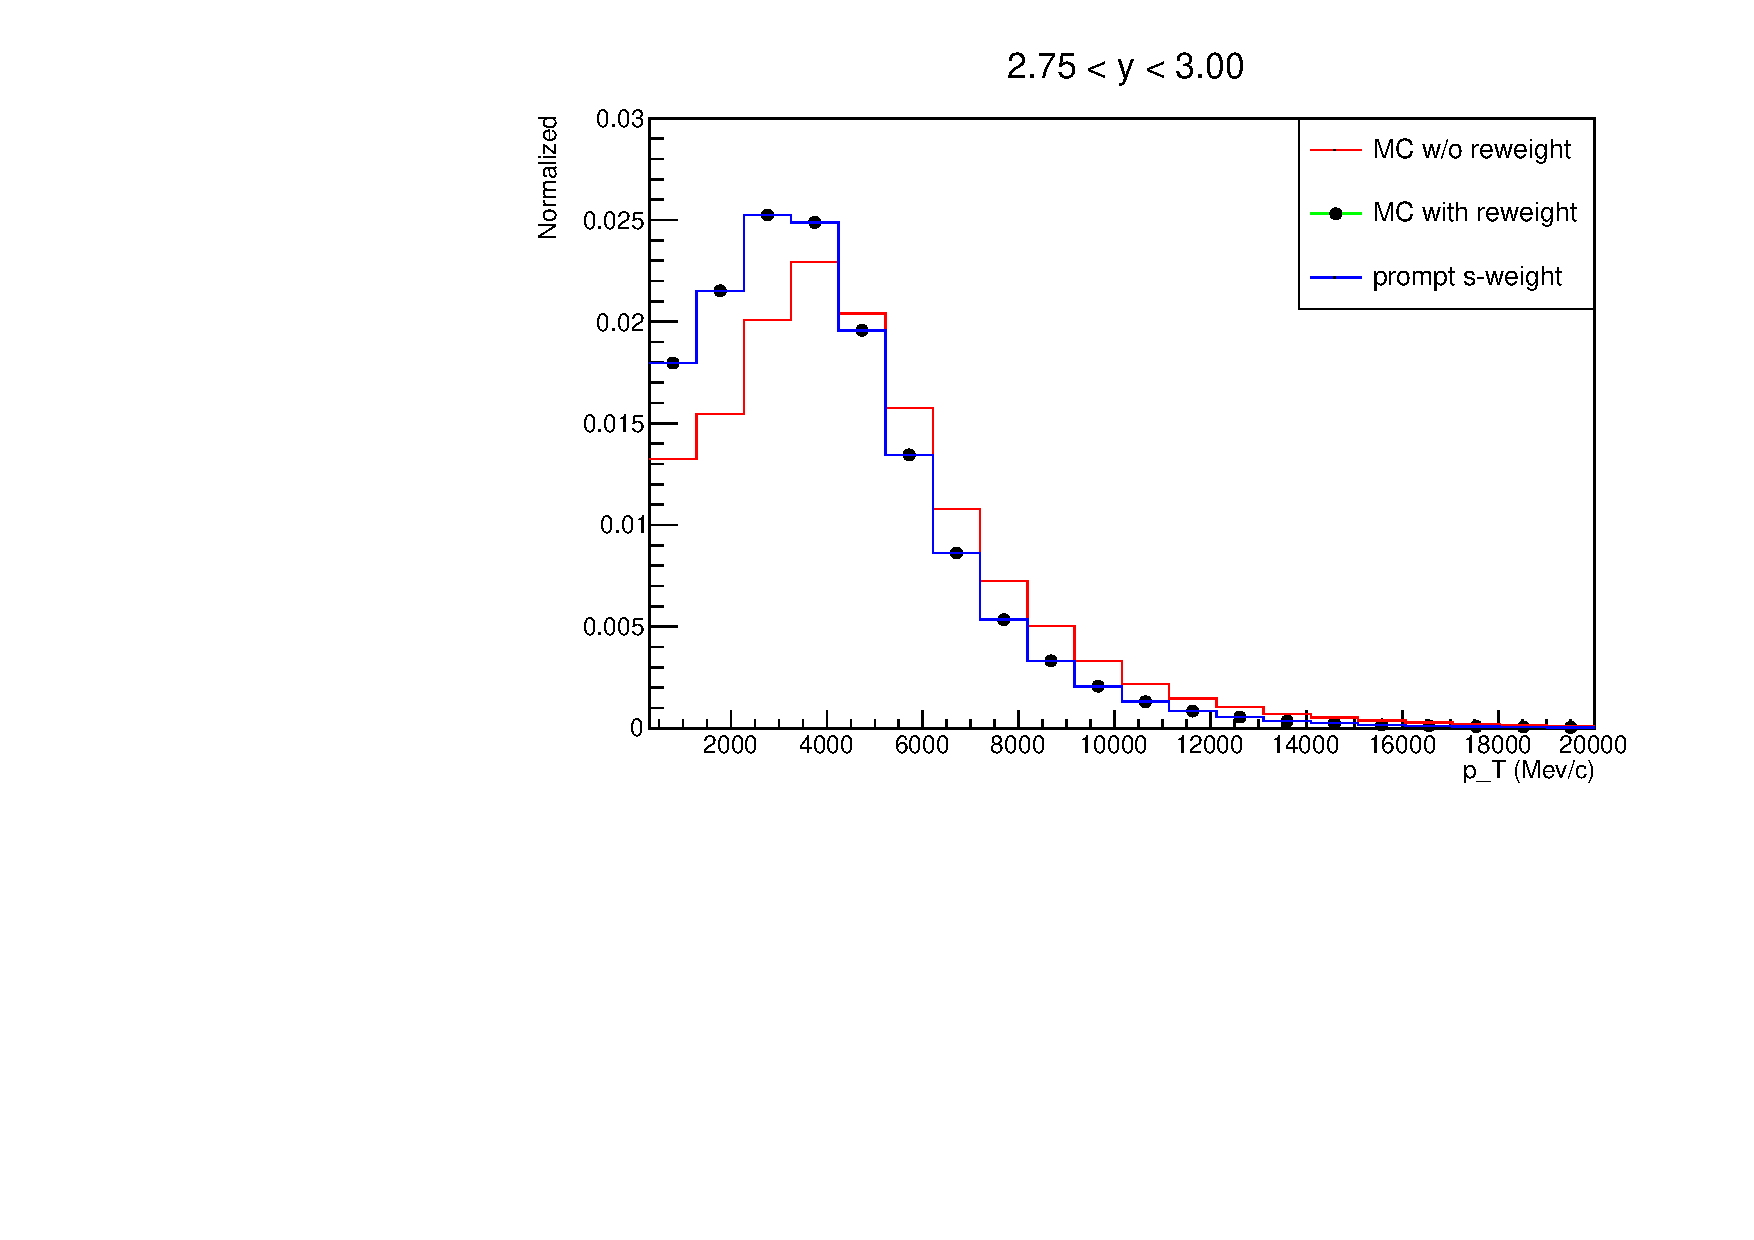
\includegraphics[width=0.19\linewidth]{pdf/Jpsi/reweight/Yp4.pdf}
      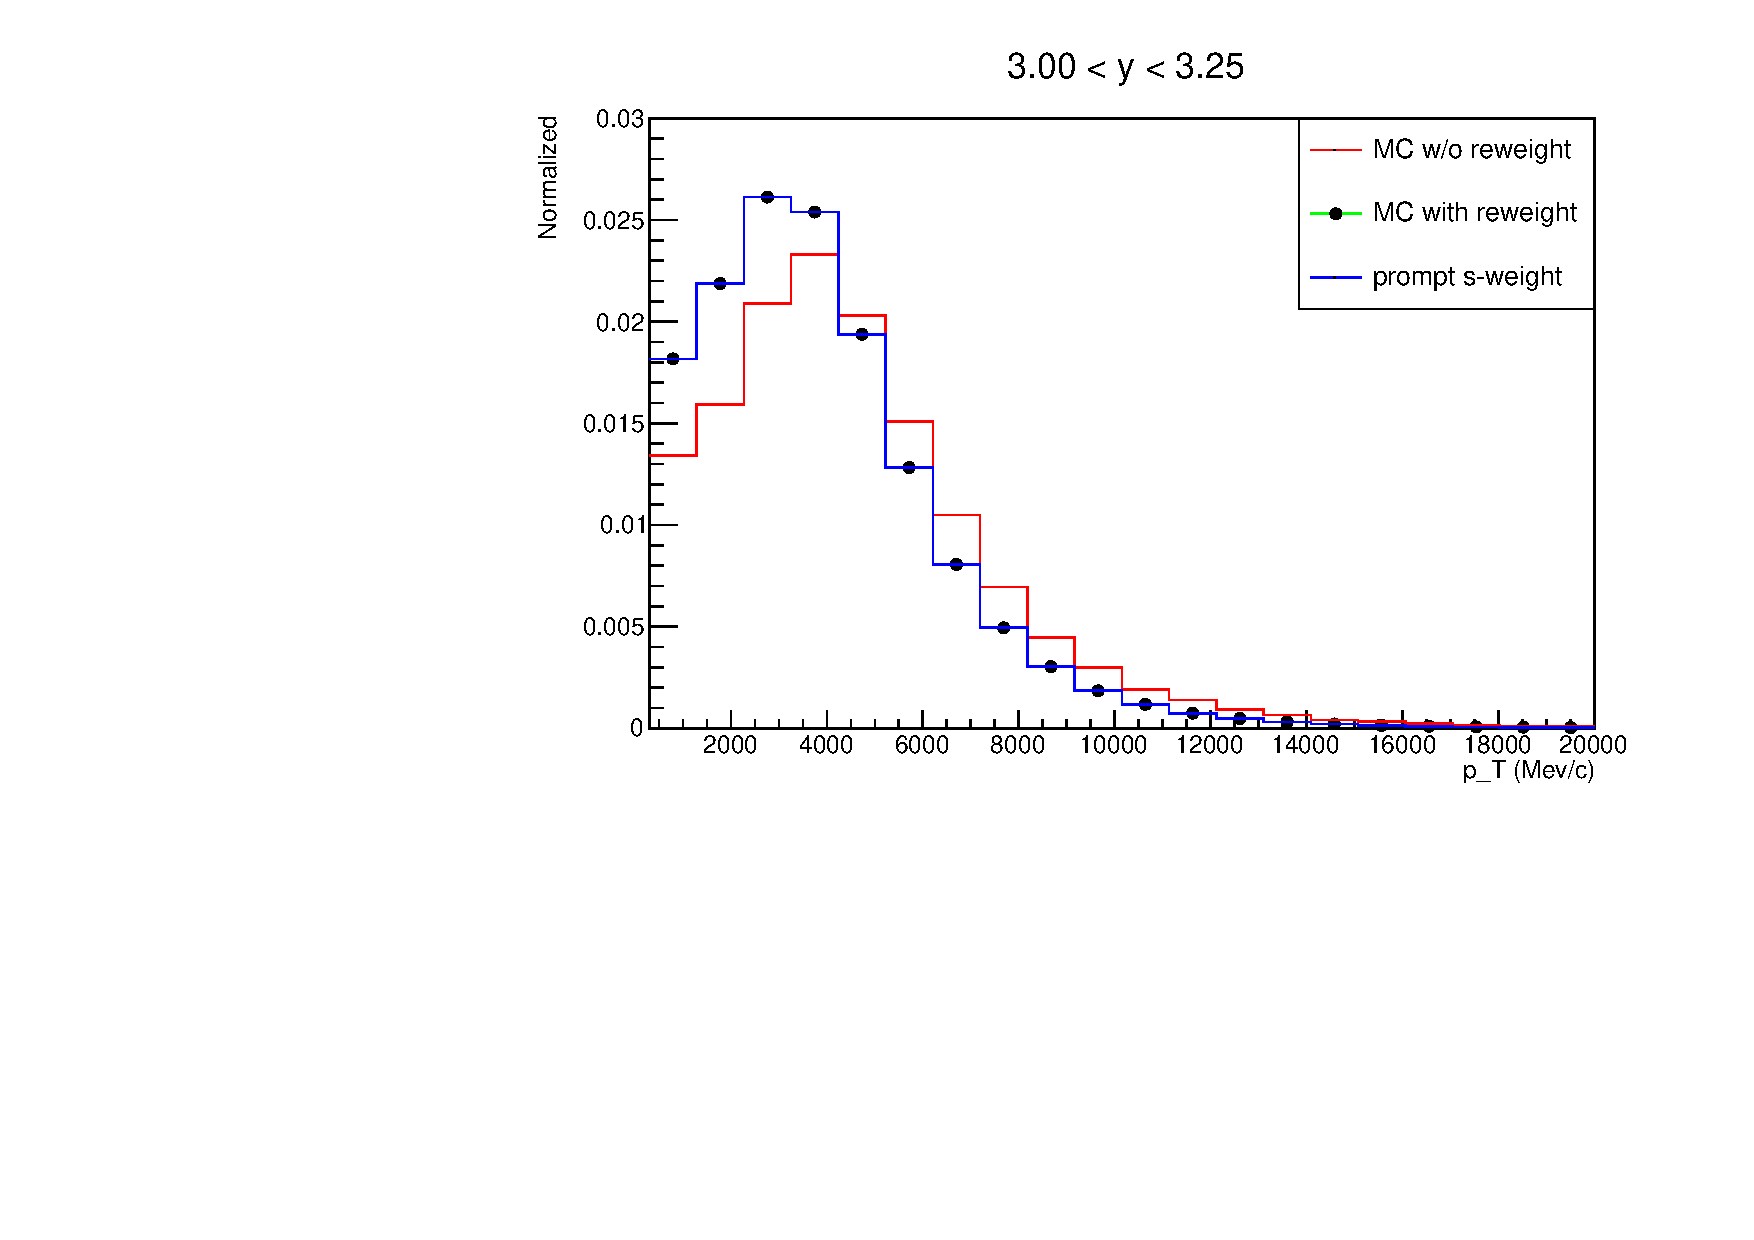
\includegraphics[width=0.19\linewidth]{pdf/Jpsi/reweight/Yp5.pdf}
      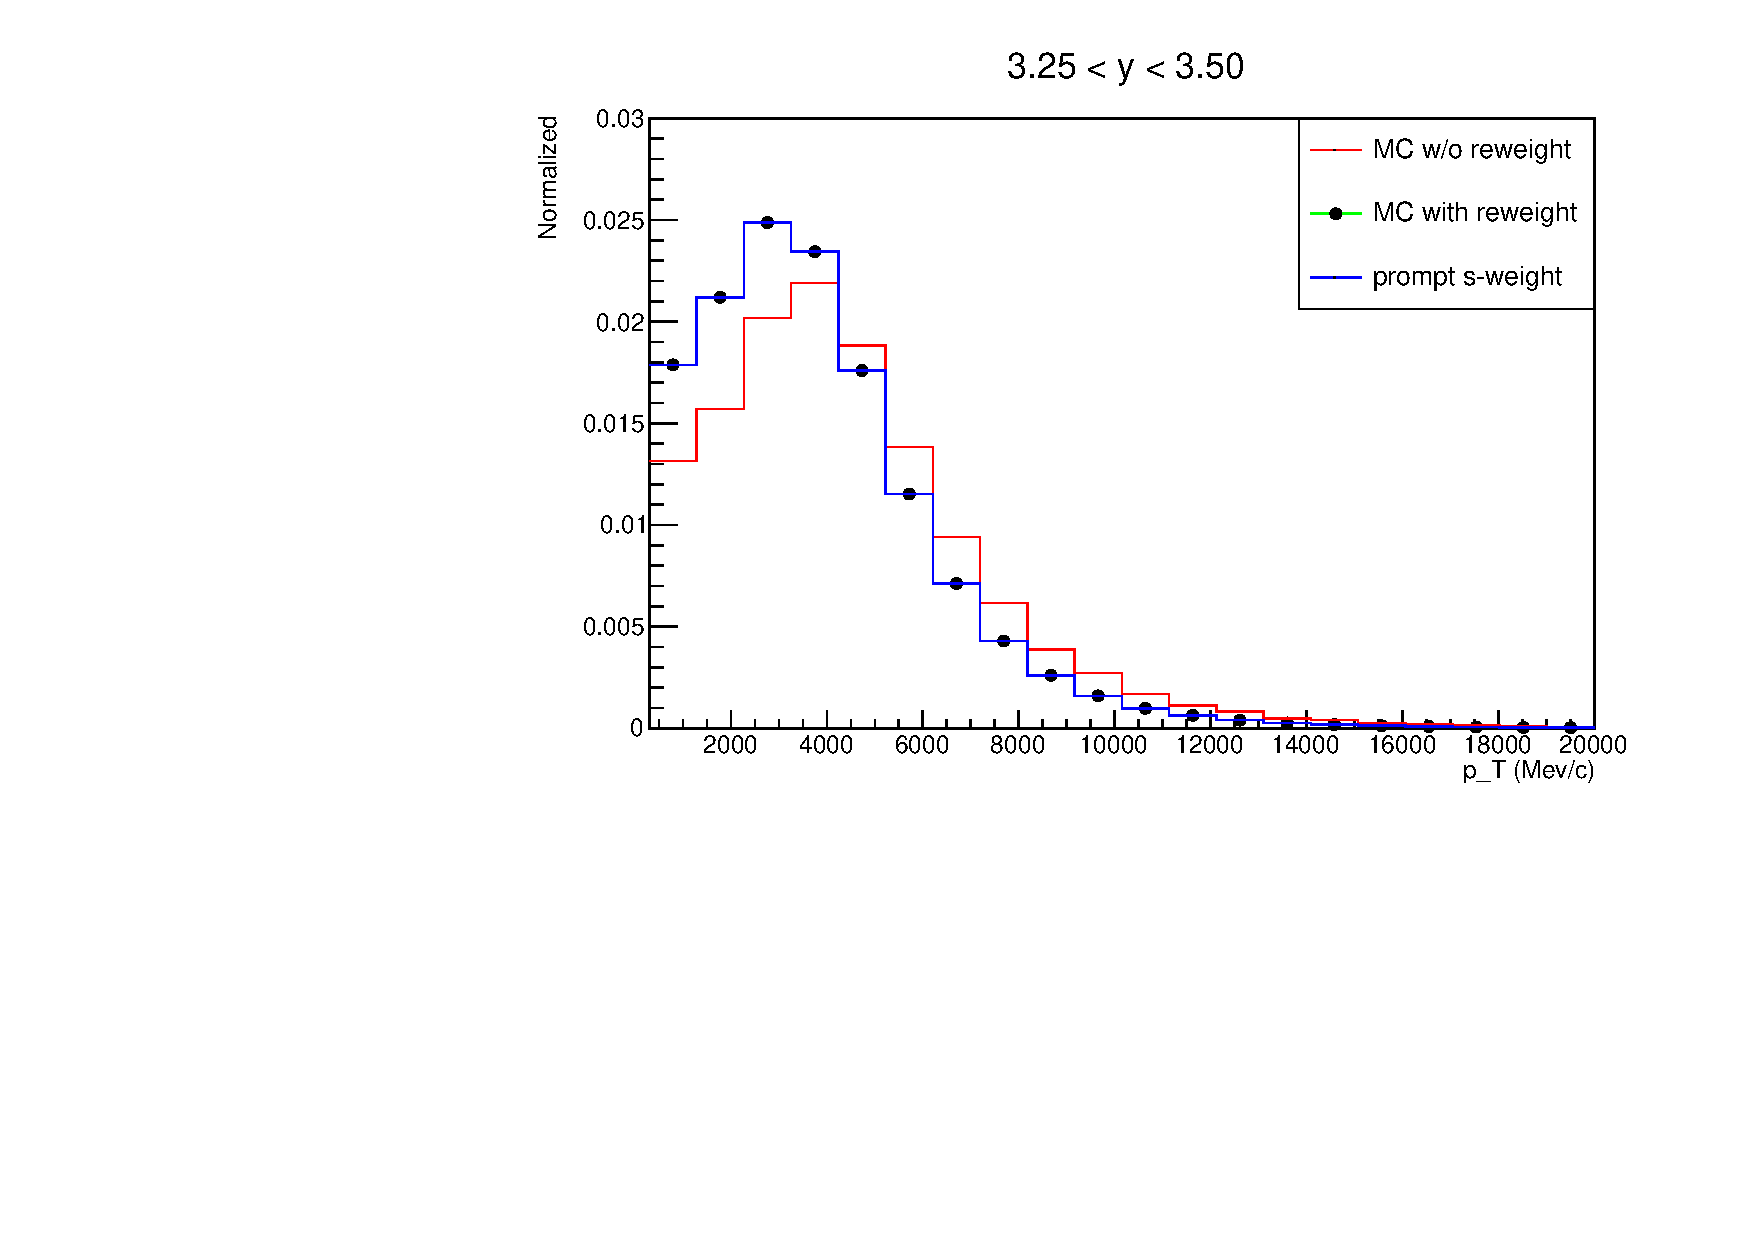
\includegraphics[width=0.19\linewidth]{pdf/Jpsi/reweight/Yp6.pdf}
      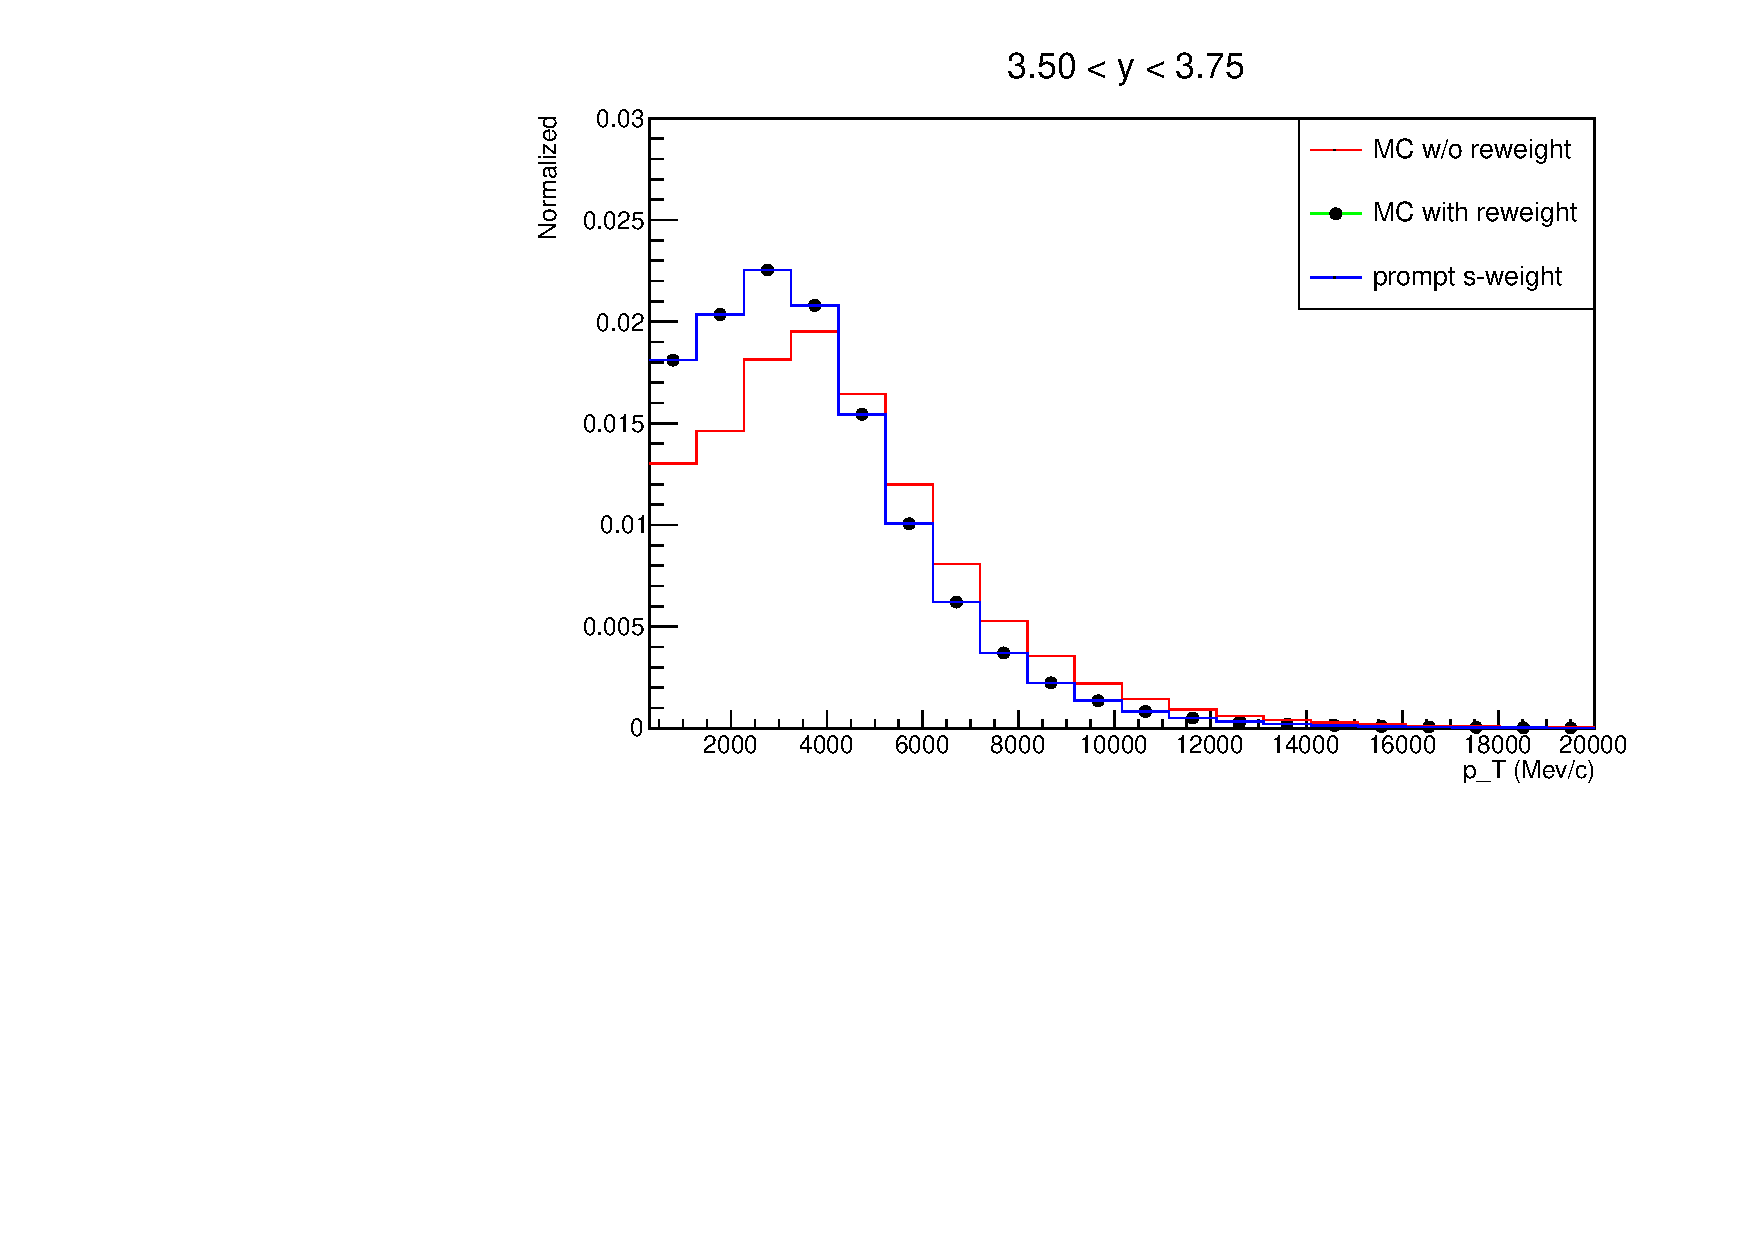
\includegraphics[width=0.19\linewidth]{pdf/Jpsi/reweight/Yp7.pdf}
	  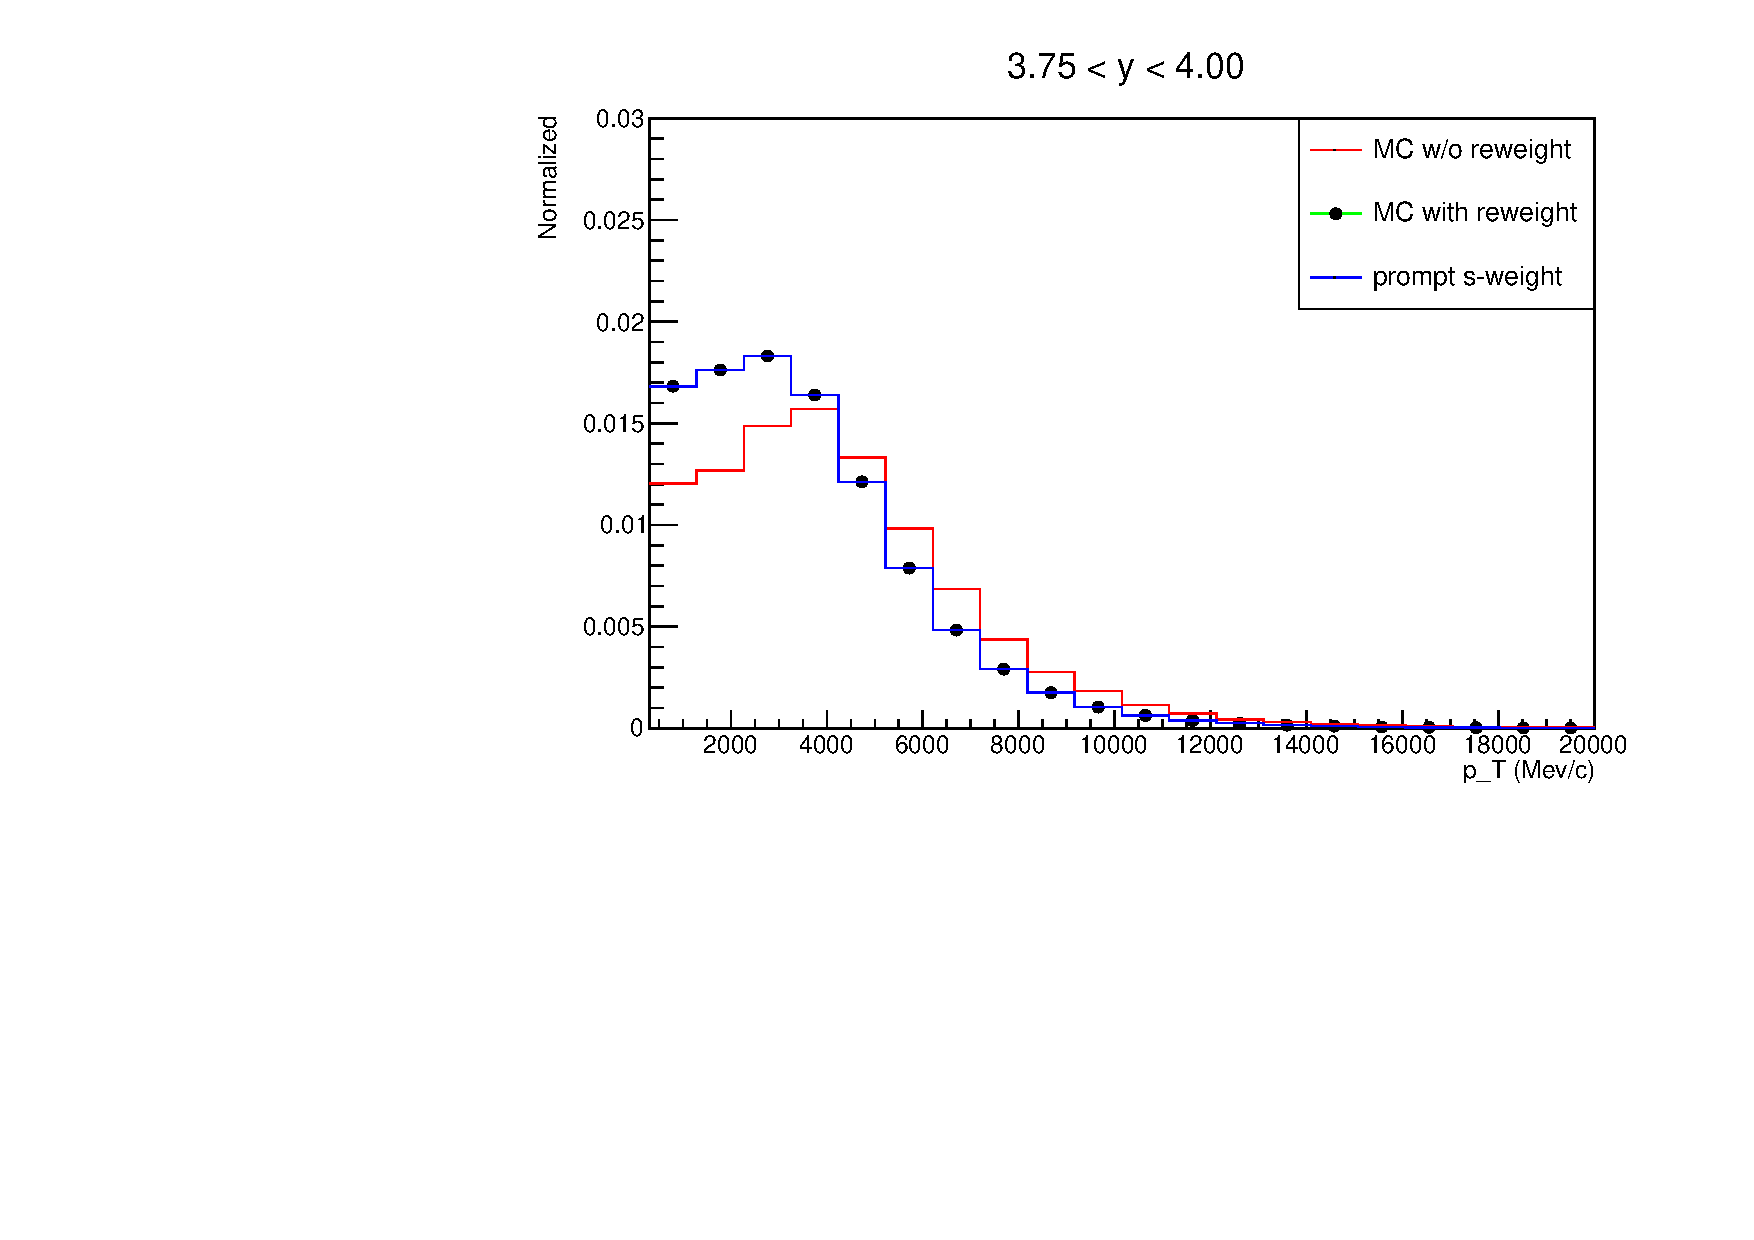
\includegraphics[width=0.19\linewidth]{pdf/Jpsi/reweight/Yp8.pdf}
      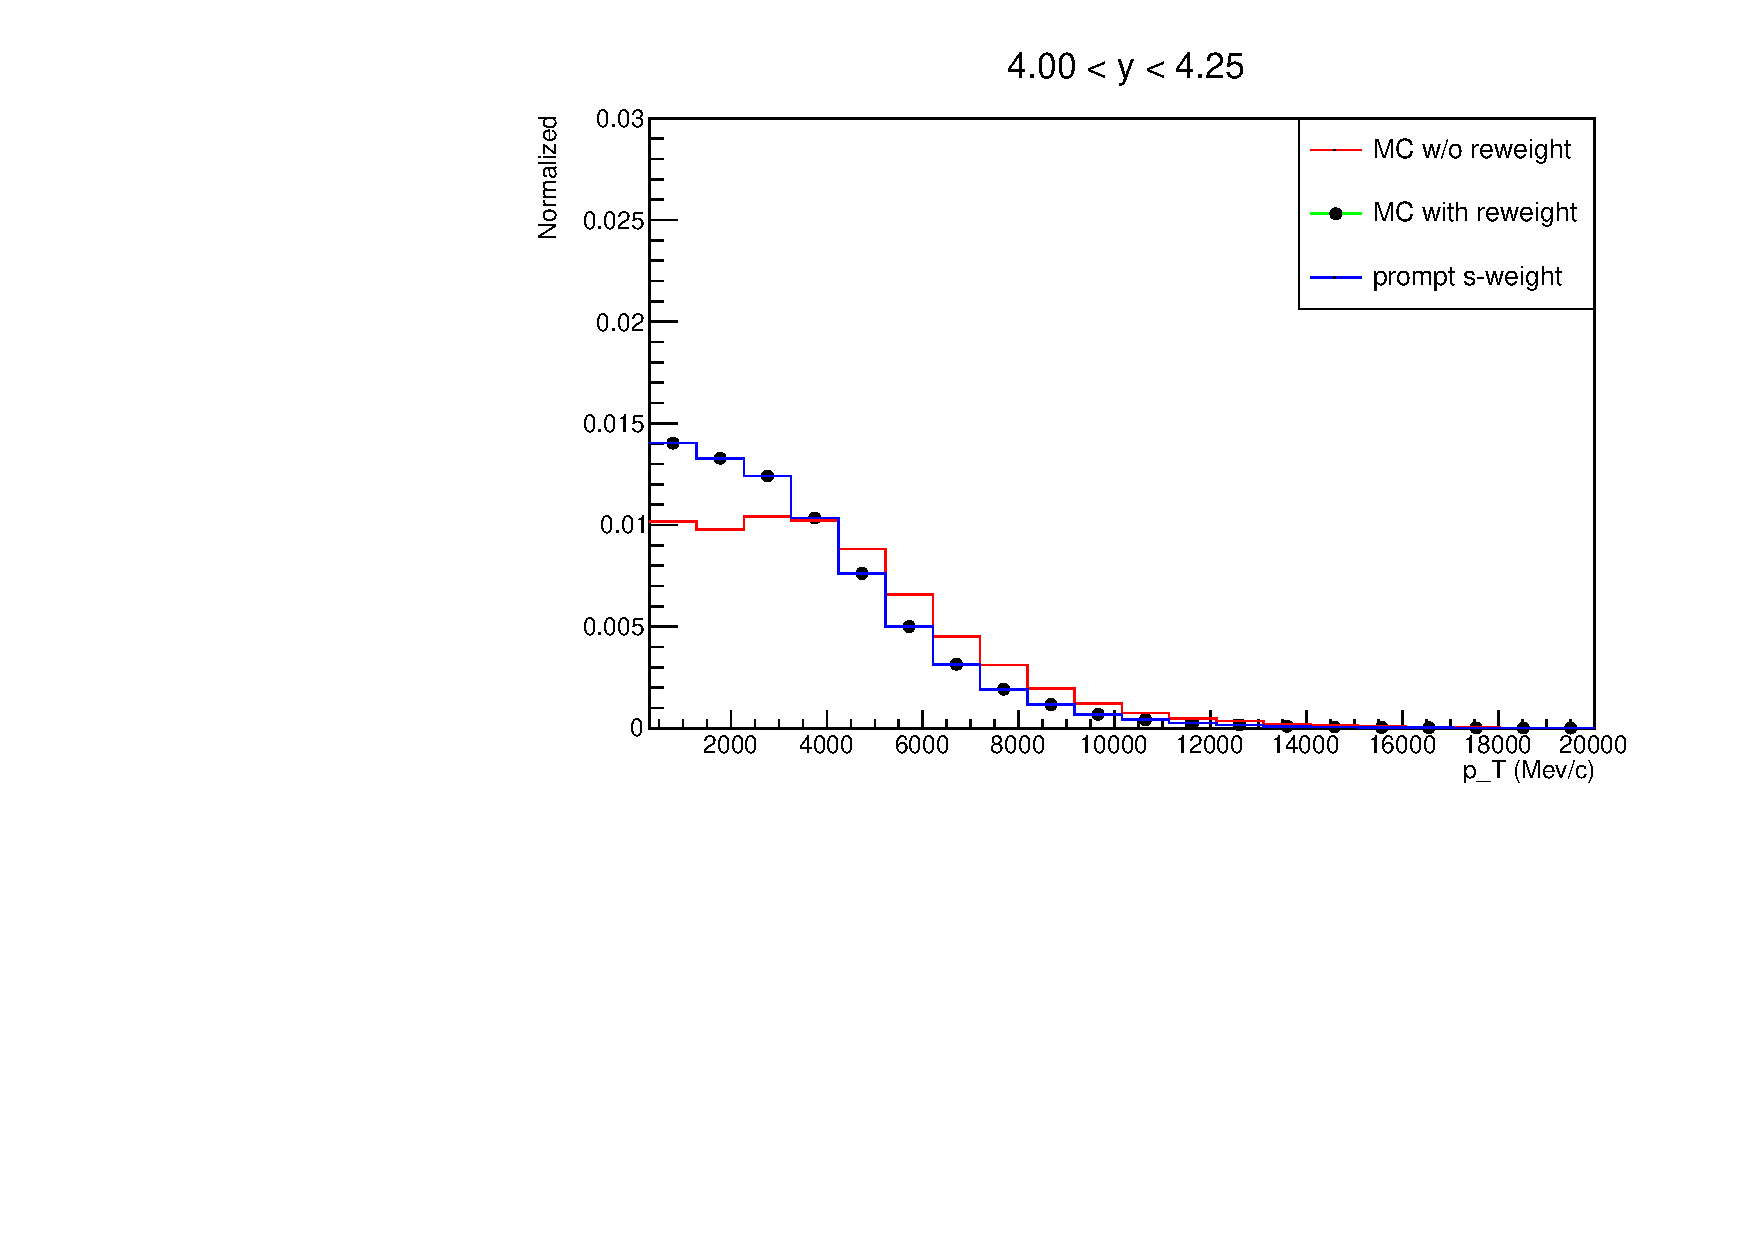
\includegraphics[width=0.19\linewidth]{pdf/Jpsi/reweight/Yp9.pdf}
      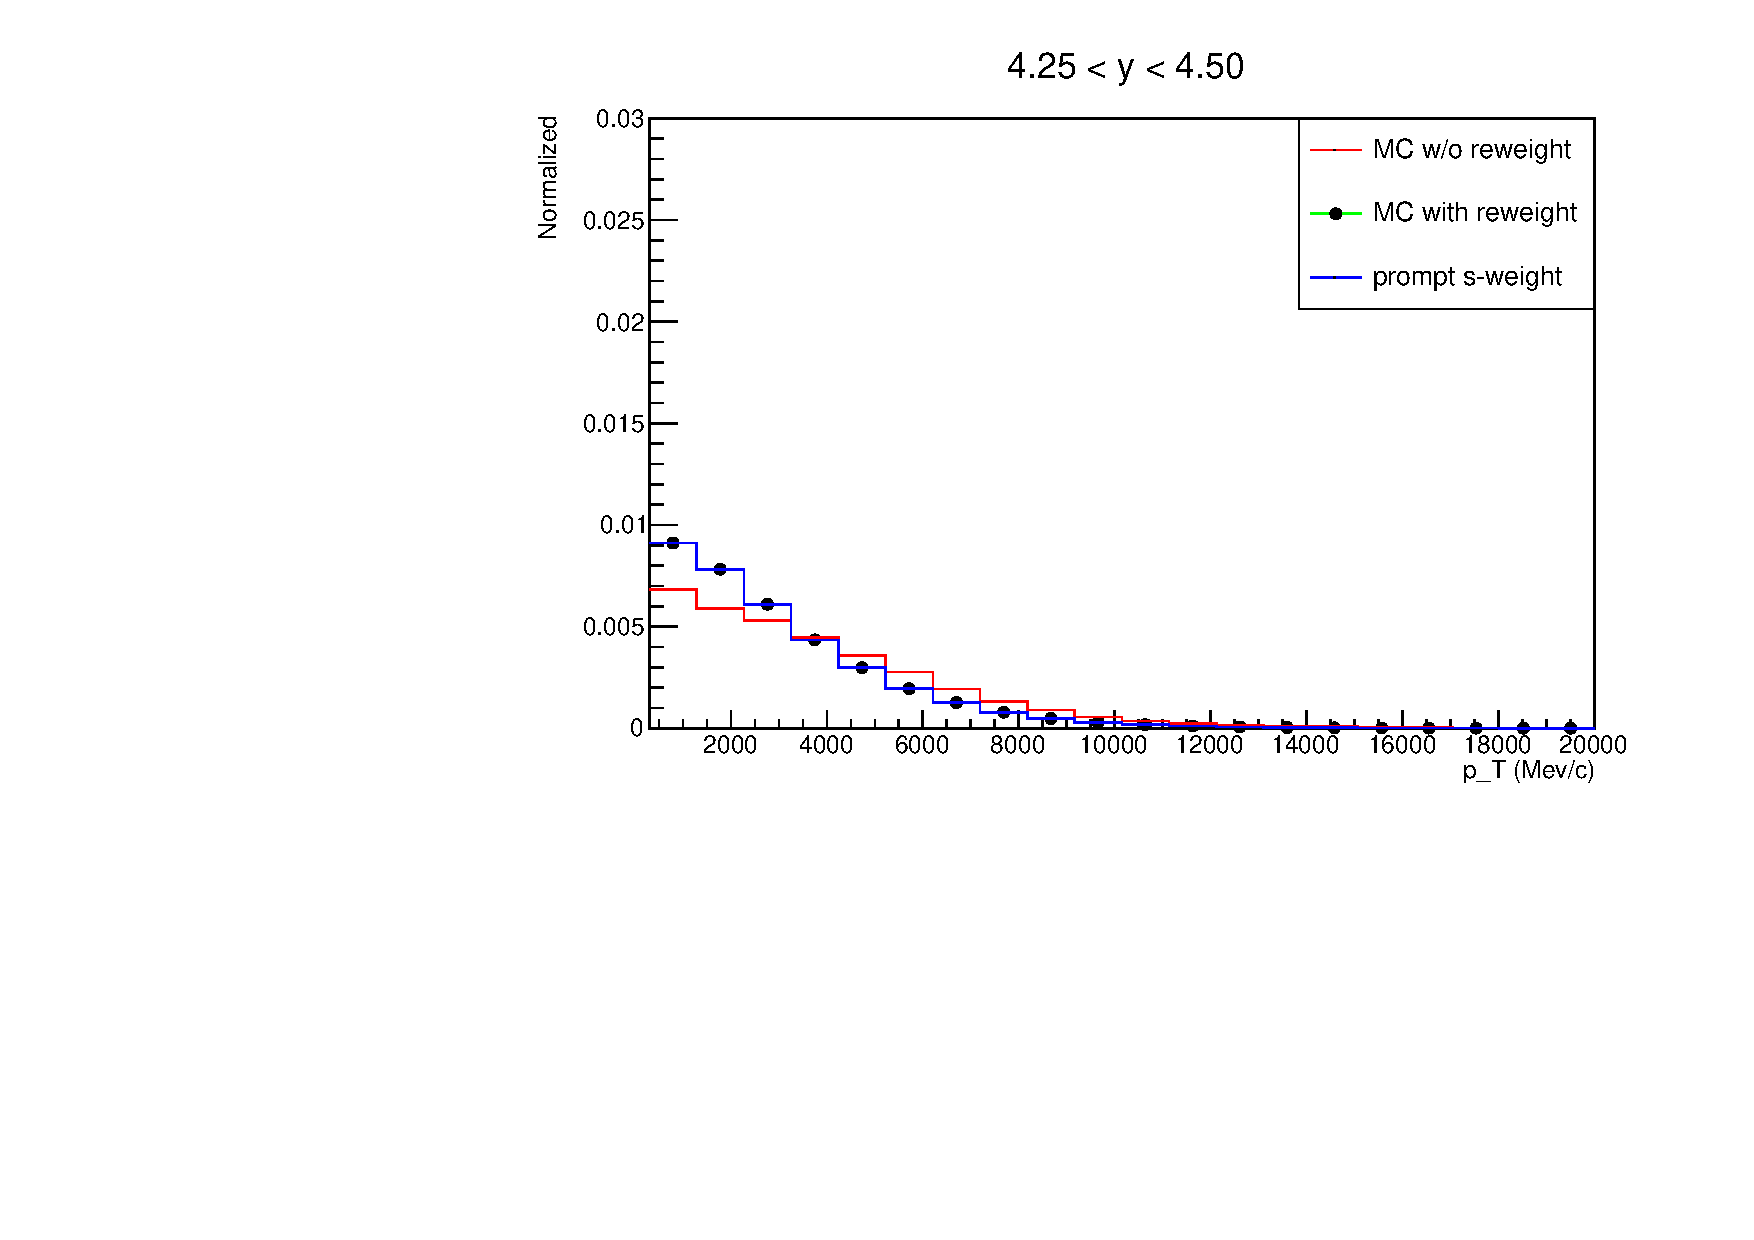
\includegraphics[width=0.19\linewidth]{pdf/Jpsi/reweight/Yp10.pdf}
	  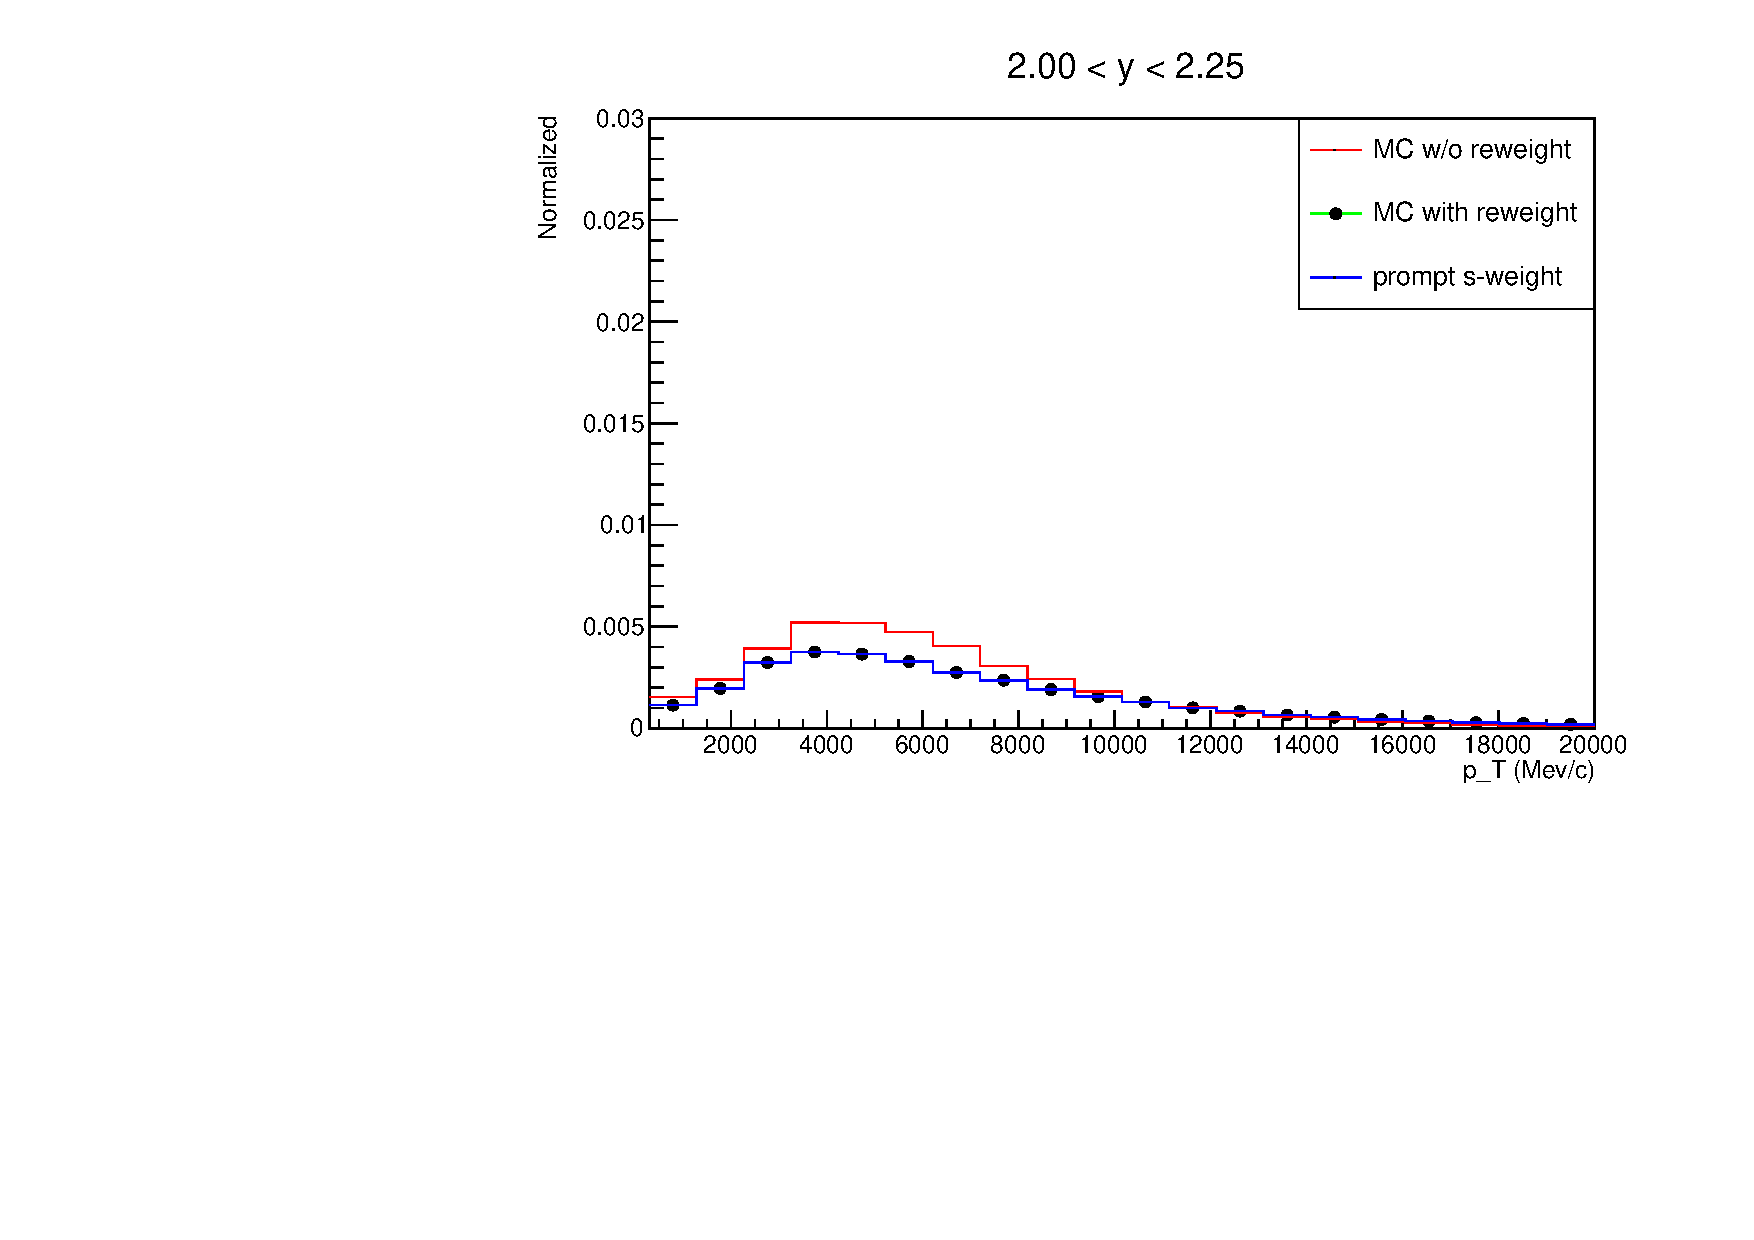
\includegraphics[width=0.19\linewidth]{pdf/Jpsi/reweight/Yb1.pdf}
      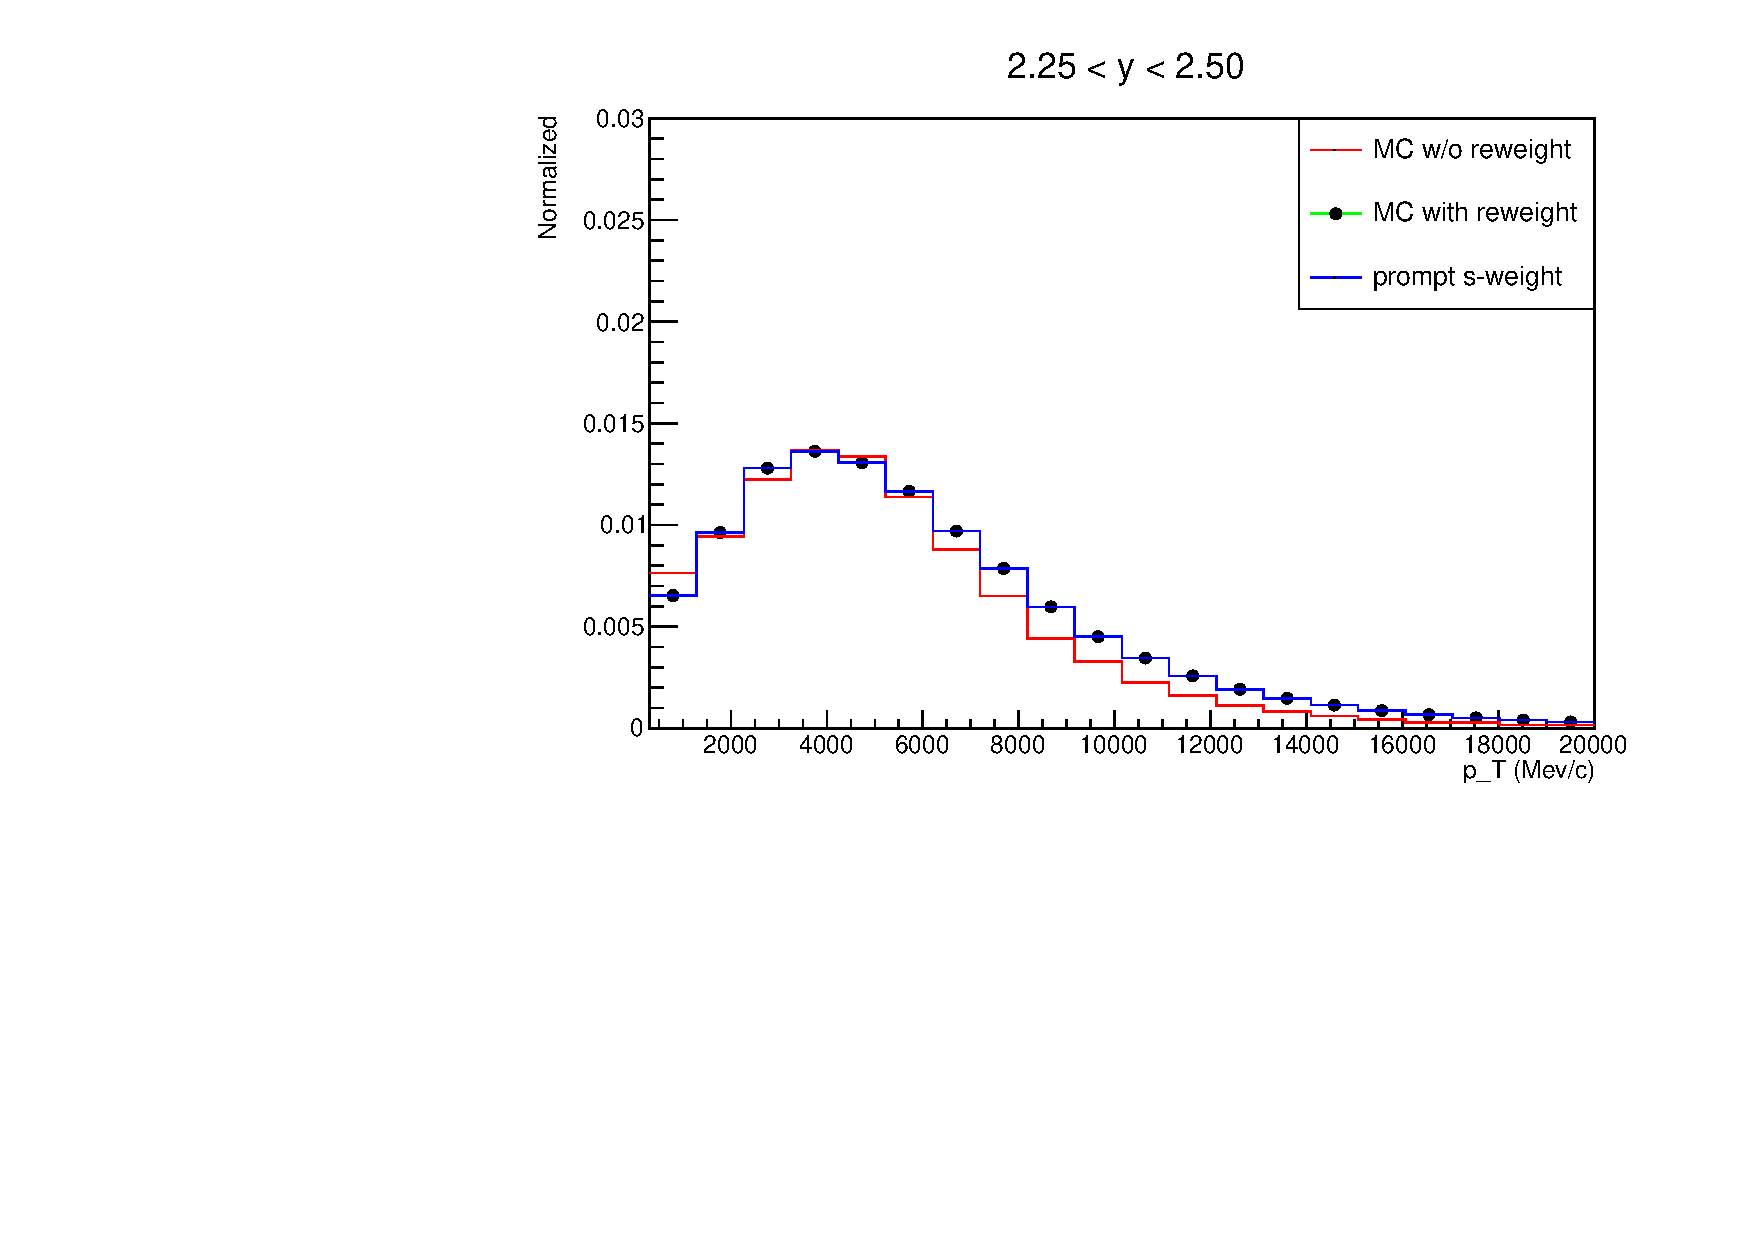
\includegraphics[width=0.19\linewidth]{pdf/Jpsi/reweight/Yb2.pdf} 
      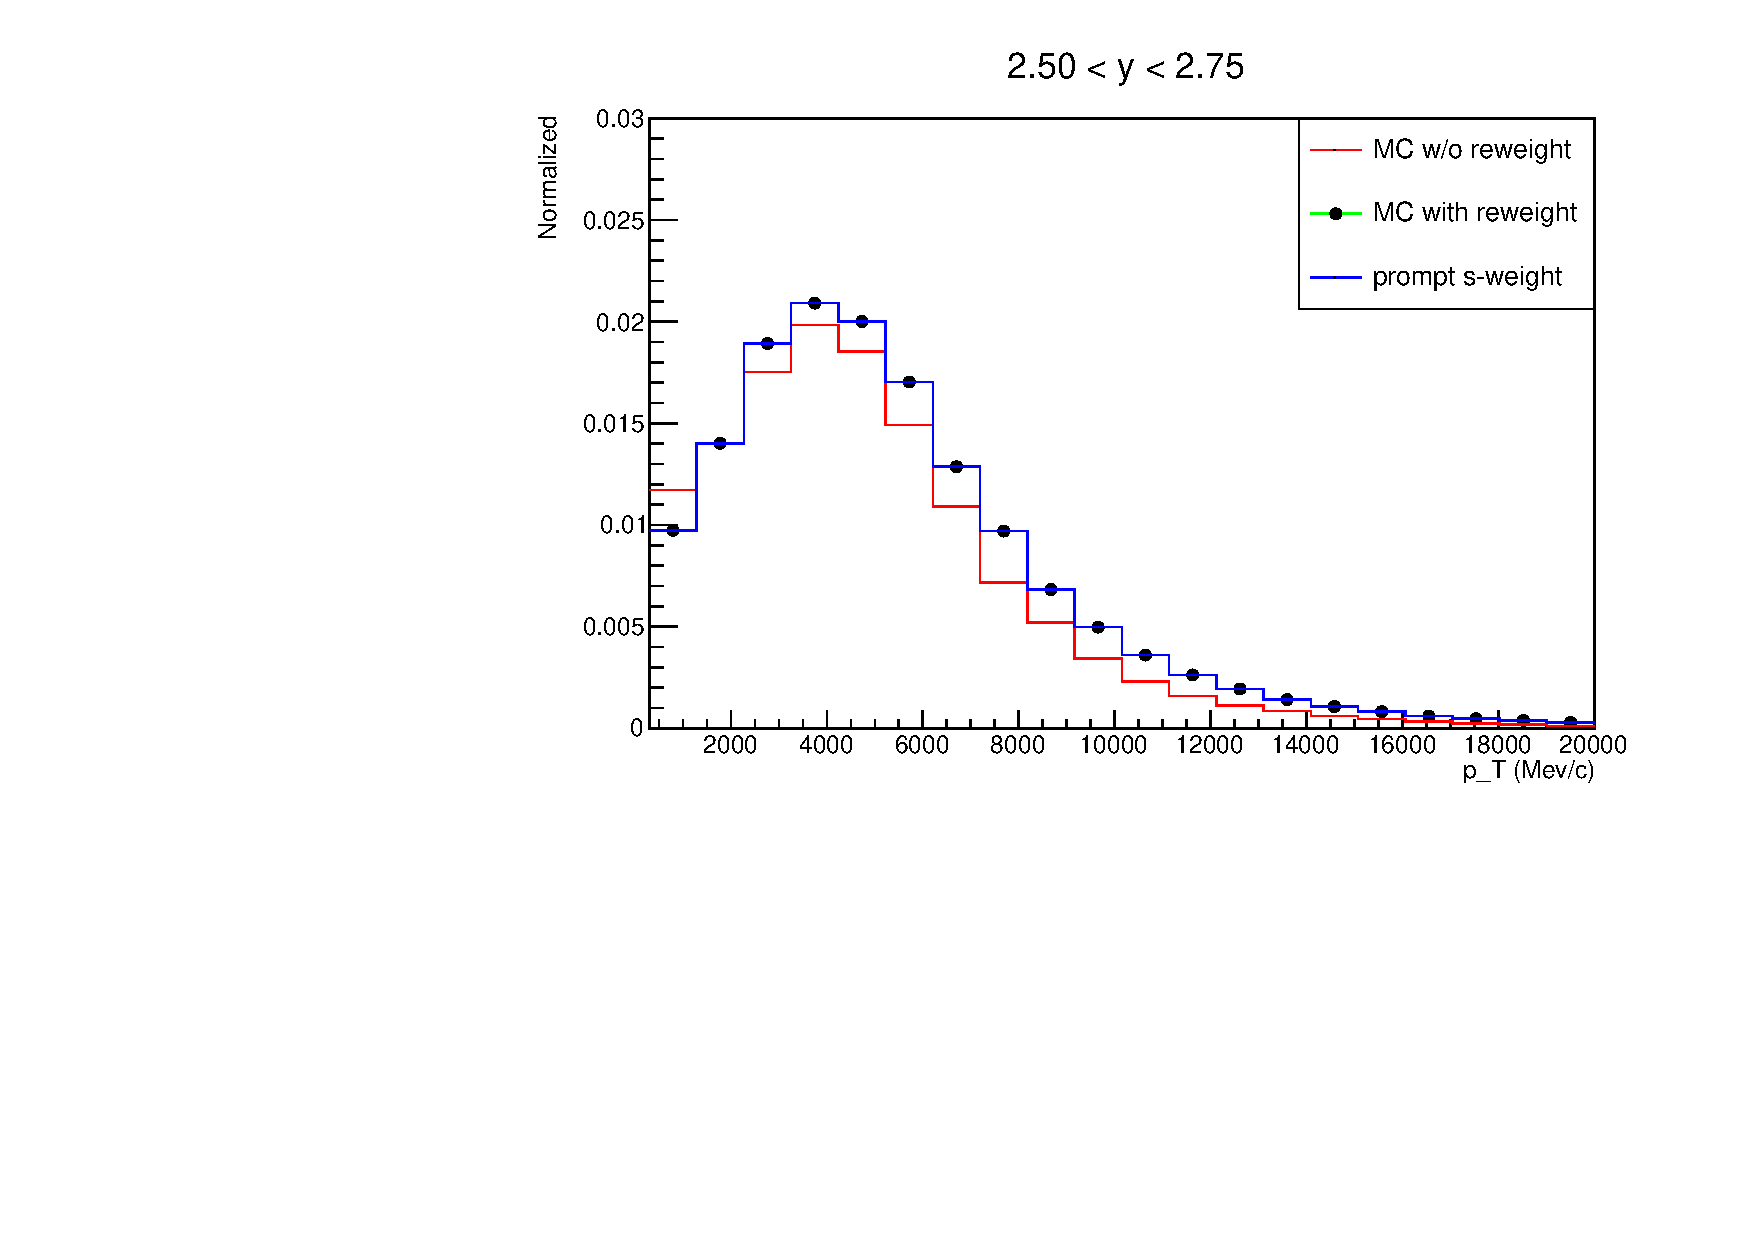
\includegraphics[width=0.19\linewidth]{pdf/Jpsi/reweight/Yb3.pdf}
      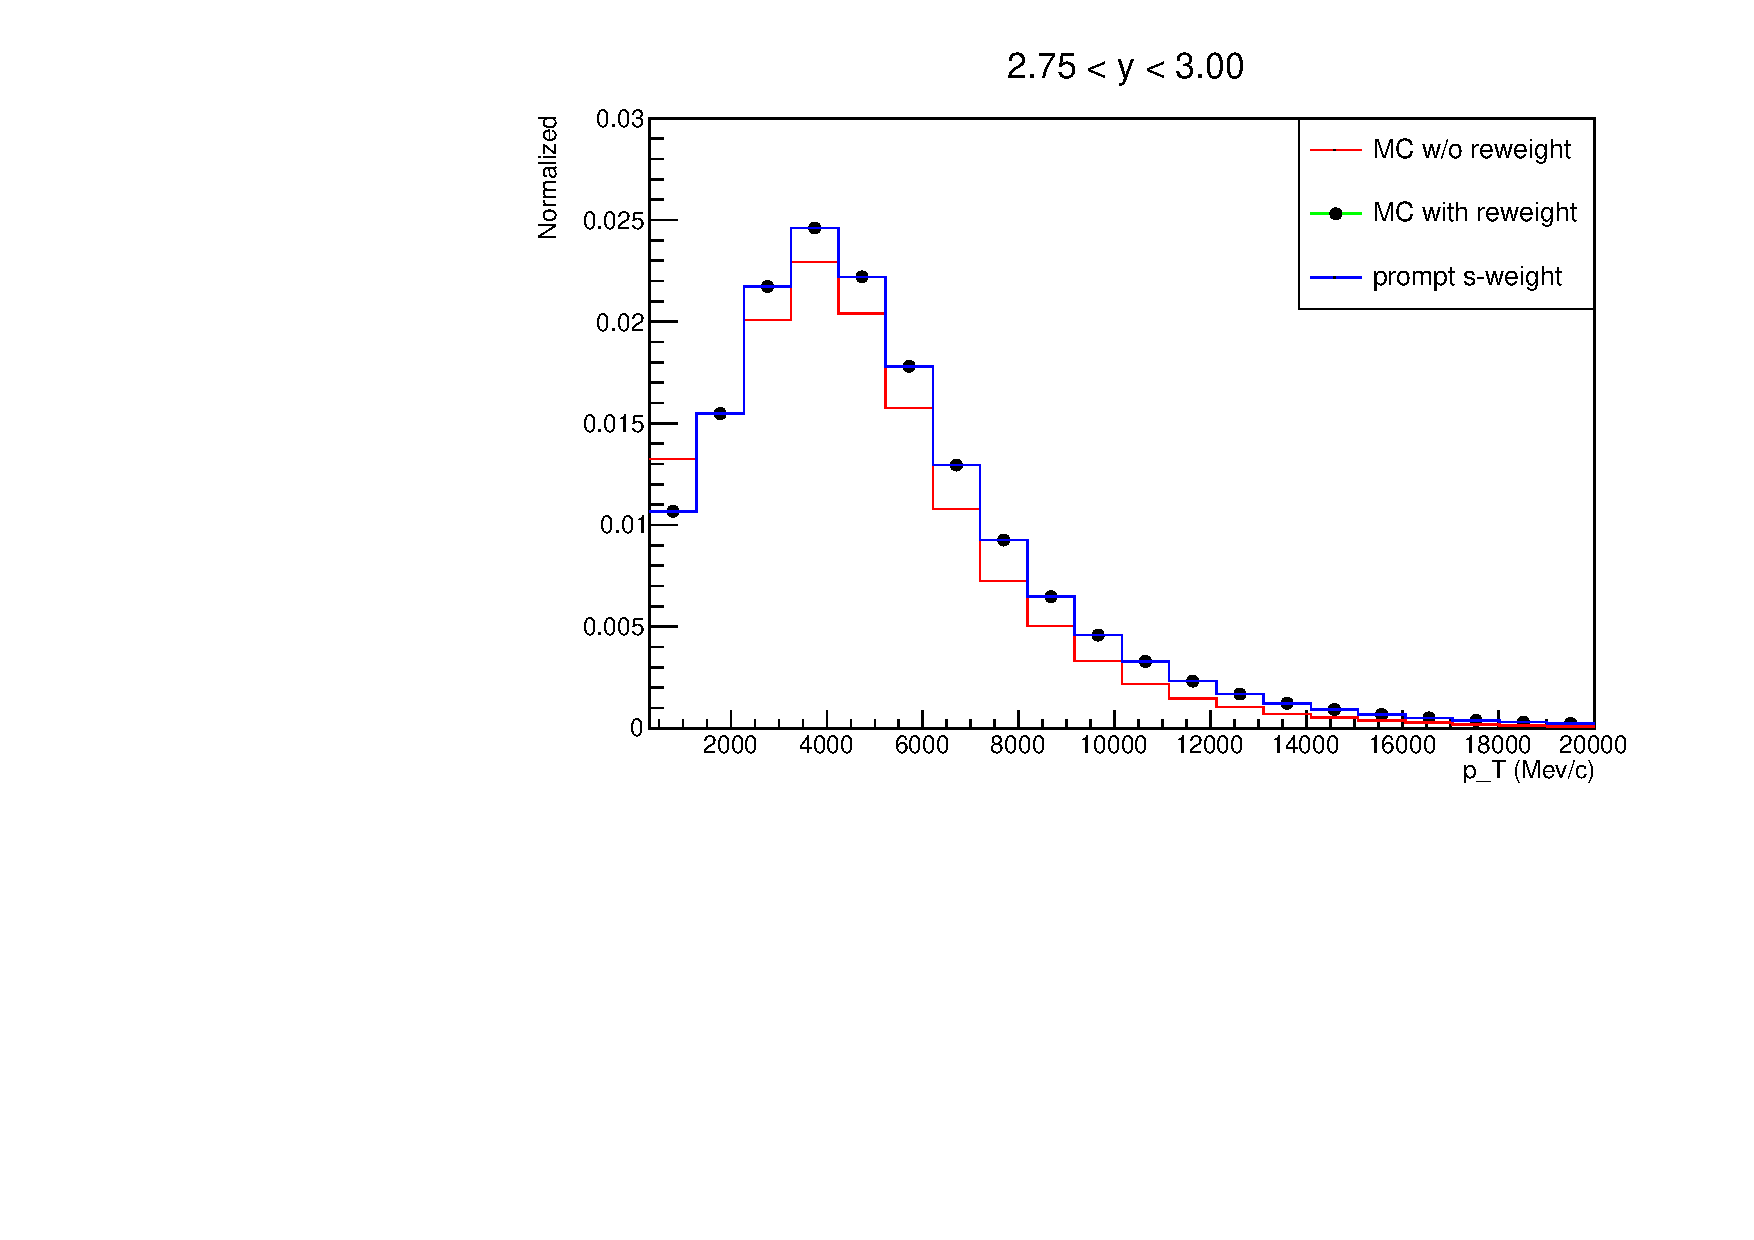
\includegraphics[width=0.19\linewidth]{pdf/Jpsi/reweight/Yb4.pdf}
      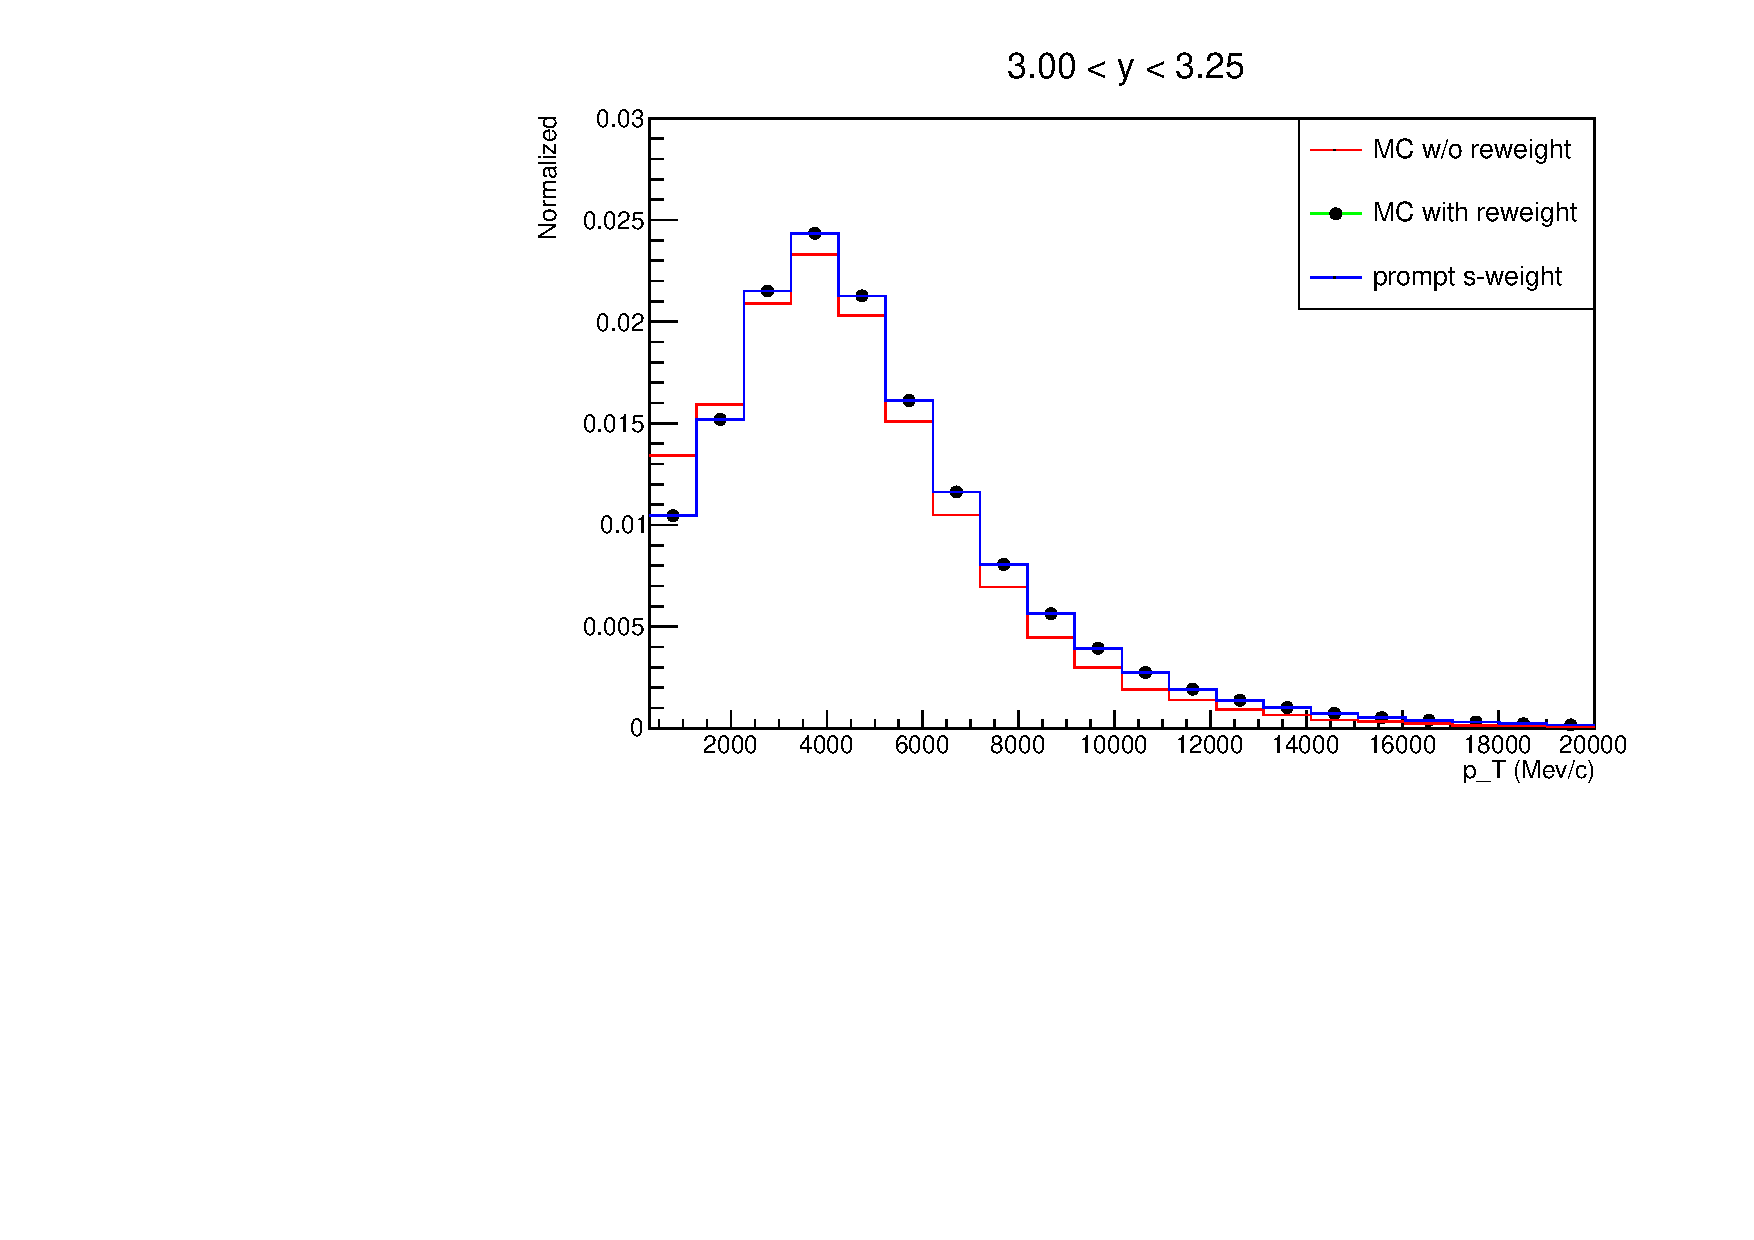
\includegraphics[width=0.19\linewidth]{pdf/Jpsi/reweight/Yb5.pdf}
      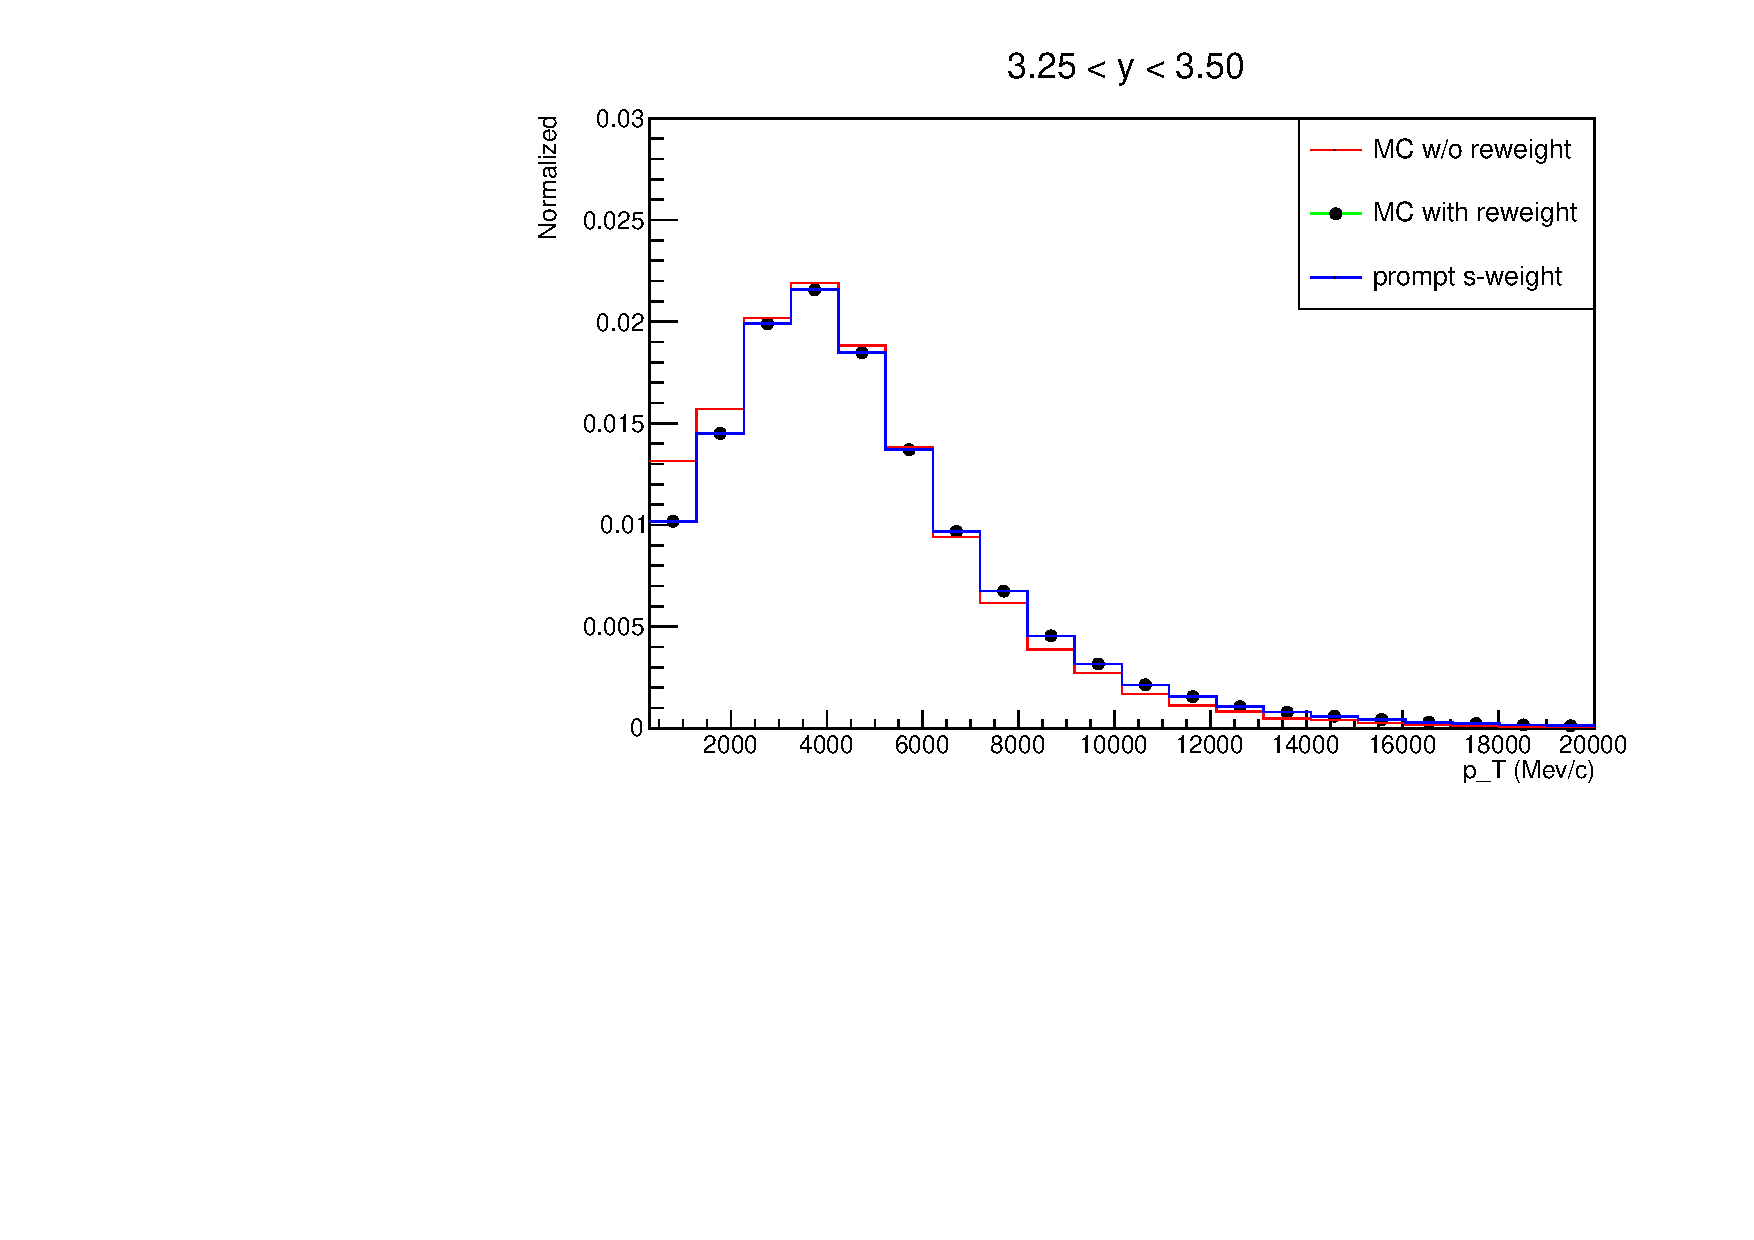
\includegraphics[width=0.19\linewidth]{pdf/Jpsi/reweight/Yb6.pdf}
      \includegraphics[width=0.19\linewidth]{pdf/Jpsi/reweight/Yb7.pdf}
      \includegraphics[width=0.19\linewidth]{pdf/Jpsi/reweight/Yb8.pdf}
      \includegraphics[width=0.19\linewidth]{pdf/Jpsi/reweight/Yb9.pdf}
      \includegraphics[width=0.19\linewidth]{pdf/Jpsi/reweight/Yb10.pdf}
    \end{center}
    \caption{
		Reweight the \pt-$y$ distribution to match MC to s-weight data. The first two rows are results of prompt \jpsi and the rest two rows are that of non-prompt \jpsi. } 
    \label{JreweightPTY}
\end{figure}
\begin{figure}[h]
    \begin{center}
      \includegraphics[width=0.19\linewidth]{pdf/Psi2S/reweight/Yp1.pdf}
      \includegraphics[width=0.19\linewidth]{pdf/Psi2S/reweight/Yp2.pdf}
      \includegraphics[width=0.19\linewidth]{pdf/Psi2S/reweight/Yp3.pdf}
      \includegraphics[width=0.19\linewidth]{pdf/Psi2S/reweight/Yp4.pdf}
      \includegraphics[width=0.19\linewidth]{pdf/Psi2S/reweight/Yp5.pdf}
      \includegraphics[width=0.19\linewidth]{pdf/Psi2S/reweight/Yp6.pdf}
      \includegraphics[width=0.19\linewidth]{pdf/Psi2S/reweight/Yp7.pdf}
      \includegraphics[width=0.19\linewidth]{pdf/Psi2S/reweight/Yp8.pdf}
      \includegraphics[width=0.19\linewidth]{pdf/Psi2S/reweight/Yp9.pdf}
      \includegraphics[width=0.19\linewidth]{pdf/Psi2S/reweight/Yp10.pdf}
      \includegraphics[width=0.19\linewidth]{pdf/Psi2S/reweight/Yb1.pdf}
      \includegraphics[width=0.19\linewidth]{pdf/Psi2S/reweight/Yb2.pdf} 
      \includegraphics[width=0.19\linewidth]{pdf/Psi2S/reweight/Yb3.pdf}
      \includegraphics[width=0.19\linewidth]{pdf/Psi2S/reweight/Yb4.pdf}
      \includegraphics[width=0.19\linewidth]{pdf/Psi2S/reweight/Yb5.pdf}
      \includegraphics[width=0.19\linewidth]{pdf/Psi2S/reweight/Yb6.pdf}
      \includegraphics[width=0.19\linewidth]{pdf/Psi2S/reweight/Yb7.pdf}
      \includegraphics[width=0.19\linewidth]{pdf/Psi2S/reweight/Yb8.pdf}
      \includegraphics[width=0.19\linewidth]{pdf/Psi2S/reweight/Yb9.pdf}
      \includegraphics[width=0.19\linewidth]{pdf/Psi2S/reweight/Yb10.pdf}
    \end{center}
    \caption{
        Reweight the \pt-$y$ distribution to match MC to s-weight data. The first two rows are results of prompt \psitwos and the rest two rows are that of non-prompt \psitwos. } 
    \label{PreweightPTY}
\end{figure}
	
%==============================================================================================================================
\subsection{Geometrical acceptance}
The geometrical acceptance in each kinematic bin is defined as
\begin{equation}
\effAcc \equiv \frac{\mbox{N($\pt$,y) with both $\mu$ in \lhcb acceptance}}{\mbox{N($\pt$,y)}}. 
\end{equation}
The \lhcb acceptance means the polar angle $[10,400]\mrad$ defined with respect to the direction of 
\lhcb $z$-axis, before the effect of the magnetic field. The efficiency $\effAcc$ is determined using 
a simulated sample at the generator level. In Fig.~\ref{EffAcc}, the efficiency in each $\pt$ and 
$y$ bin of \jpsi and \psitwos mesons for $PVZ>-60mm$ and $nPVs=1$ are presented. The geometrical acceptances 
for prompt production and production from $b$-hadron decay are calculated separately for both \jpsi and 
\psitwos. And since the geometrical acceptance is only a function of kinematic variables, we assume that 
there is no difference between the geometrical acceptance between different multiplicity regions.

\begin{figure}[!tbp]
  \begin{center}
    \includegraphics[width=0.49\linewidth]{pdf/Jpsi/eff_acc/eff_prompt_point.pdf}
    \includegraphics[width=0.49\linewidth]{pdf/Psi2S/eff_acc/eff_prompt_point.pdf}
    \vspace*{-0.5cm}
    \includegraphics[width=0.49\linewidth]{pdf/Jpsi/eff_acc/eff_fromb_point.pdf}
    \includegraphics[width=0.49\linewidth]{pdf/Psi2S/eff_acc/eff_fromb_point.pdf}
  \end{center}
  \caption{
    Efficiency of geometrical acceptance for both \jpsi and \psitwos for PVNTRACKS in 4 to 20, where the 
    left is that of \jpsi and the right is of \psitwos. The first row is that of prompt signals and the 
    second row is that of non-prompt signals.}
  \label{EffAcc}
\end{figure}

%==============================================================================================================================
\subsection{Reconstruction-selection efficiency}
The reconstruction and selection efficiency in each kinematic bin is estimated as
\begin{equation}
\effReco  \equiv \frac{\mbox{N($\pt$,y) reconstructed and selected (w/o $\mu$ ID)}}{\mbox{N($\pt$,y) with both $\mu$ in LHCb acceptance}}.
\end{equation}
It includes the efficiency of reconstructing the two muon tracks and the selection of the signals, with the selection criteria listed in Table~\ref{Table32} (excluding muon identification and the trigger). 
Then the reconstruction efficiency is further corrected using the data-over-simulation single tracking efficiency ratio.
The ratio of tracking efficiencies for a single track in data and simulation determined with the Long Tag-Probe method~\cite{LHCb-DP-2013-002} is shown in Fig.~\ref{TrackEfficiencyCalib}, which was given by the tracking group.
\begin{figure}[H]
  \begin{center}
    \includegraphics[width=0.8\linewidth]{pdf/TrackCalib.pdf}
  \end{center}
  \caption{
    Tracking efficiency ratio between data and MC2016 simulation in bins of $p_{\mu}$ and $\eta_{\mu}$ 
    of the muon.}
  \label{TrackEfficiencyCalib}
\end{figure}
For a given event the correction factor is determined by multiplying the efficiency ratios for each of the tracks in the final state. The reweight for prompt and non-prompt signals are done separately with the sWeight extracted from two-dimensional fit. 
For each $\pt$ and $y$ bin, the efficiency of \effReco is shown in Fig.~\ref{EffRec} for PVNTRACKS between 4 to 20. Results in other multiplicity regions are shown in Sec~\ref{sec:EffTables}.
\begin{figure}[!tbp]
  \begin{center}
    \includegraphics[width=0.49\linewidth]{pdf/Jpsi/eff_rec_sel/n1_eff_rec_sel_prompt_point.pdf}
    \includegraphics[width=0.49\linewidth]{pdf/Psi2S/eff_rec_sel/n1_eff_rec_sel_prompt_point.pdf}
    \vspace*{-0.5cm}
    \includegraphics[width=0.49\linewidth]{pdf/Jpsi/eff_rec_sel/n1_eff_rec_sel_fromb_point.pdf}
    \includegraphics[width=0.49\linewidth]{pdf/Psi2S/eff_rec_sel/n1_eff_rec_sel_fromb_point.pdf}
  \end{center}
  \caption{
    Efficiency of reconstruction and selection (excluding muon identification and the trigger) for both \jpsi and \psitwos for PVNTRACKS in 4 to 20, where the 
    left is that of \jpsi and the right is of \psitwos. The first row is that of prompt signals and the 
    second row is that of non-prompt signals.}
  \label{EffRec}
\end{figure}
%==============================================================================================================================
\subsection{Muon identification efficiency}
The muon identification requirement used in this analysis is ${\rm IsMuon}==1\&\& {\rm DLLmu}>2 \&\& {\rm ProbNNmu}>0.8$. 
The efficiency is introduced by 
\begin{equation}
\effID    \equiv \frac{\mbox{N($\pt$,y) selected including $\mu$ID requirement}}{\mbox{N($\pt$,y) reconstructed and selected (w/o $\mu$ID)}}.
\end{equation}

The Muon ID efficiency is obtained using simulated samples and calibrated with the data using the PIDCalib package.
The full simulated samples used here are selected by all the selections except the muon ID and the trigger.
The selected samples are the same as the ones used in the reconstruction and selection.
As estimating the reconstruction and selection efficiency, we first reweight the multiplicity variable according to the variable we used to divide the multiplicity, and \pt-$y$ spectrum.
The muon ID efficiency in each (\pt,$y$) bin is then calculated by averaging the muon ID efficiency of each candidate in the bin, which is the product of the muon ID efficiencies of the two muons from the efficiency table, obtained from the PIDCalib package, according to their $(p,\eta,{\rm nSPDhits})$ values. 
The formula is
\begin{equation}
\overline{\epsilon}(\pt,y)=\frac{\sum \epsilon_\mup(p_\mup,\eta_\mup,\mathrm{nSPDhits})\epsilon_\mun(p_\mun,\eta_\mun,\mathrm{nSPDhits})}{N_\mathrm{res\&sel}}.
\label{eq:muonid}
\end{equation}
where $\epsilon_\mup(p_\mup,\eta_\mup,\mathrm{nSPDhits})$ and $\epsilon_\mun(p_\mun,\eta_\mun,\mathrm{nSPDhits})$ are the muon ID efficiencies obtained from the efficiency table.
The efficiency table we used here is from the calibration sample which contains \jpsi candidates taken in the same period and the average efficiency over the whole period is used.
One 3-Dimensional efficiency table dedicated to the muon ID selection is obtained from this calibration sample in bins of the muon $\mathrm{(p,\eta,\mathrm{nSPDhits})}$ using the tag-and-probe method.
The MagDown and MagUp efficiencies are calculated separately.
For the muon candidates whose $(p, \eta,\mathrm{nSPDhits})$ are out of the range of the calibration sample, we simply set the value to be one due to the fact that the production in those bins is significantly small.
For each $\pt$ and $y$ bin, the efficiency of \effID is shown in Fig.~\ref{EffID}. Results in other multiplicity regions are shown in Sec~\ref{sec:EffTables}.
\begin{figure}[!tbp]
  \begin{center}
    \includegraphics[width=0.49\linewidth]{pdf/Jpsi/eff_pid/n1_eff_pid_prompt_point.pdf}
    \includegraphics[width=0.49\linewidth]{pdf/Psi2S/eff_pid/n1_eff_pid_prompt_point.pdf}
    \vspace*{-0.5cm}
    \includegraphics[width=0.49\linewidth]{pdf/Jpsi/eff_pid/n1_eff_pid_fromb_point.pdf}
    \includegraphics[width=0.49\linewidth]{pdf/Psi2S/eff_pid/n1_eff_pid_fromb_point.pdf}
  \end{center}
  \caption{
    PID efficiencies for both \jpsi and \psitwos for PVNTRACKS in 4 to 20, where the 
    left is that of \jpsi and the right is of \psitwos. The first row is that of prompt signals and the 
    second row is that of non-prompt signals.}
  \label{EffID}
\end{figure}
%==============================================================================================================================
\subsection{Trigger efficiency}
The trigger efficiency in each kinematic bin is defined as 
\begin{equation}
\effTrigger \equiv \frac{\mbox{N($\pt$,y) triggered}}{\mbox{N($\pt$,y) selected including $\mu$ID requirement}} 
\end{equation}
Here the triggers include both TOS requirements of \texttt{L0DiMuon}, \texttt{Hlt1DiMuonHighMass} for both, and \texttt{Hlt2DiMuonJPsiTurbo} for \jpsi and \texttt{Hlt2DiMuonPsi2STurbo} for \psitwos, respectively. 
Only \texttt{L0DiMuon} and \texttt{Hlt1DiMuonHighMass} contribute actually to the efficiency because the \texttt{Hlt2DiMuonJPsiTurbo} and \texttt{Hlt2DiMuonPsi2STurbo} is almost fully efficient due to the facts that the offline selections are tighter.
For each $\pt$ and $y$ bin, the efficiencies of \effTrigger for both \jpsi and \psitwos from different sources for PVNTRACKS between 4 to 20 are shown in Fig.~\ref{EffTrigger}. Results in other multiplicity regions are shown in Sec~\ref{sec:EffTables}.
\begin{figure}[!tbp]
  \begin{center}
    \includegraphics[width=0.49\linewidth]{pdf/Jpsi/eff_trigger/n1_eff_trigger_prompt_point.pdf}
    \includegraphics[width=0.49\linewidth]{pdf/Psi2S/eff_trigger/n1_eff_trigger_prompt_point.pdf}
    \vspace*{-0.5cm}
    \includegraphics[width=0.49\linewidth]{pdf/Jpsi/eff_trigger/n1_eff_trigger_fromb_point.pdf}
    \includegraphics[width=0.49\linewidth]{pdf/Psi2S/eff_trigger/n1_eff_trigger_fromb_point.pdf}
  \end{center}
  \caption{
    Trigger efficiencies for both \jpsi and \psitwos for PVNTRACKS in 4 to 20, where the 
    left is that of \jpsi and the right is of \psitwos. The first row is that of prompt signals and the 
    second row is that of non-prompt signals.}
  \label{EffTrigger}
\end{figure}
%==============================================================================================================================
\subsection{Total efficiency}
The total efficiencies \effTot for \jpsi and \psitwos from different sources for PVNTRACKS between 4 to 20 are shown in Fig.~\ref{EffTot}. Results in other multiplicity regions are shown in Sec~\ref{sec:EffTables}.
The separate efficiencies for prompt and non-prompt signals are used to calculate the final cross-section.
\begin{figure}[!tbp]
  \begin{center}
    \includegraphics[width=0.49\linewidth]{pdf/Jpsi/eff_tot/n1_prompt_point.pdf}
    \includegraphics[width=0.49\linewidth]{pdf/Psi2S/eff_tot/n1_prompt_point.pdf}
    \vspace*{-0.5cm}
    \includegraphics[width=0.49\linewidth]{pdf/Jpsi/eff_tot/n1_fromb_point.pdf}
    \includegraphics[width=0.49\linewidth]{pdf/Psi2S/eff_tot/n1_fromb_point.pdf}
  \end{center}
  \caption{
    Total efficiencies for both \jpsi and \psitwos for PVNTRACKS in 4 to 20, where the 
    left is that of \jpsi and the right is of \psitwos. The first row is that of prompt signals and the 
    second row is that of non-prompt signals.}
  \label{EffTot}
\end{figure}

\subsection{Variation due to different reweight samples}
Since the multiplicity-dependent breakup effects may vary with (\pt, $y$), the two-dimensional (\pt, $y$) distribution may differ in different multiplicity region. To study this effect, the (\pt, $y$) spectra are prepared for three different multiplicity classes:
\begin{itemize}
	\item Data sample with all selections of PVNTRACKS.
	\item Data sample with PVNTRACKS$>=60$ as high-multiplicity sample, where 60 is the bin edge of the second to last bin of \pt binning scheme.
	\item Data sample with PVNTRACKS$<60$ as low-multiplicity sample.
\end{itemize}	
 The (\pt,$y$) distributions of high- and low-multiplicity samples are shown in Figs.~\ref{HighLowDist}. 
With this two samples for (\pt, $y$) reweight, we can calculate the ratio of total efficiencies for both prompt and non-prompt \jpsi and \psitwos in each multiplicity region. And after comparing the newly calculated ratio of total efficiencies with the original one, we record the variation in each (\pt, $y$, PVNTRACKS) bin in form of a certain time of statistical uncertainty in that bin. And the result is shown in Figs~\ref{HighLow}. It's clearly shown that all the variations are within uncertainties, where the center values and uncertainties for ratio of efficiencies are from the results reweighted by the full-multiplicity sample.
\begin{figure}[h]
  \begin{center}
    \includegraphics[width=0.49\linewidth]{pdf/Jpsi/reweight/promptHighLowPTY.pdf}
    \includegraphics[width=0.49\linewidth]{pdf/Psi2S/reweight/promptHighLowPTY.pdf}
    \vspace*{-0.5cm}
    \includegraphics[width=0.49\linewidth]{pdf/Jpsi/reweight/frombHighLowPTY.pdf}
    \includegraphics[width=0.49\linewidth]{pdf/Psi2S/reweight/frombHighLowPTY.pdf}
  \end{center}
  \caption{
    Two-dimensional (\pt, $y$) distribution for prompt and non-prompt \jpsi and \psitwos of different samples (high-multiplicity sample in red).}
  \label{HighLowDist}
\end{figure}

\begin{figure}[h]
  \begin{center}
	  \includegraphics[width=0.6\linewidth]{pdf/HighLow.pdf}
  \end{center}
\caption{
	Distribution of the variation due to different reweight samples recorded in times of the statistical uncertainty.}
\label{HighLow}
\end{figure}


\section{Systematic Uncertainties}
\def\effTri{\ensuremath{\epsilon_{\mathrm{trigger}}}\xspace}
\def\effTotJ{\ensuremath{\epsilon_{\mathrm{tot,\jpsi}}}\xspace}
\def\effTotP{\ensuremath{\epsilon_{\mathrm{tot,\psitwos}}}\xspace}
\def\pandb{prompt components and components from $b$-hadron decay}
The ratio of production of \psitwos to \jpsi in a certain $(\pt,y)$ is 
defined in equation ~\ref{Rsingle}, which is universal for both prompt components and components from $b$-hadron decay in each multiplicity bin and
Systematic uncertainties of various sources are combined through the error propagation formula in each bin.
While when calculating the systematic uncertainties of the ratio of integrated production, the bin size is 
no more canceled and we need to take into account the production as weight in each bin. The ratio of integrated 
production is defined in equation ~\ref{Rintegrated}.

The form of expression for the ratio of integrated production is not a simple production or division (it is a division of sums). So when studying the systematic uncertainties, 
a simple and straightforward way is calculating the uncertainties of $\frac{\Sigma_{(\pt,y)}\sigma_{\psitwos}(\pt,y)}{\Sigma_{(\pt,y)}\sigma_{\jpsi}(\pt,y)}$ itself, 
which is for example, if we calculate the uncertainty of the fit model, instead of combining the uncertainties from 
different bins, we directly calculate how much $\frac{\Sigma_{(\pt,y)}\sigma_{\psitwos}(\pt,y)}{\Sigma_{(\pt,y)}\sigma_{\jpsi}(\pt,y)}$ 
would vary when we change the fit model. For the uncertainties which are independent of bins, we can 
combine them through the error propagation formula, i.e. the Systematic uncertainty due to MC sample size.
The following sources of systematic uncertainties are considered. And the systematic uncertainties are calculated 
separately in each multiplicity bin.
For the rest of the part, we only show the results for the first multiplicity bin, which is 4$\leq$PVNTRACKS$<$20. 
%=============================================================================================
\subsection{Signal extraction}
\subsubsection{Signal mass shape}
\label{sec:masssyst}
Using the sum of two Crystal Ball functions parametrized as described in Section~\ref{Signal Extraction} could bias the signal yields.
For an alternative, the signal invariant mass is also fitted with the model which is extracted from the kernel-estimated distribution from the simulated sample bin dependently. 
In order to account for the resolution difference between data and simulation, a Gaussian function (all the parameters float during the fit procedure) is used to smear the shape of the signals.
The study is performed in each kinematic bin, and the signal yields from the default fit and alternative fit are compared.
For both \jpsi and \psitwos, we change the fit model to get uncertainties for both and then calculate the uncertainties through the error propagation formula.
The detailed results of systematic uncertainty for ratio in each single $\pt$ and $y$ bin and PVNTRACKS from 4 to 20 are shown in Fig.~\ref{sys_mass}.
The result is common for both prompt components and components from $b$-hadron decay since when we fit the mass spectrum, we fit both components simultaneously. 
\begin{figure}[!tbp]
    \begin{center}
      \includegraphics[width=0.49\linewidth]{pdf/SysMPlot/n1Err_point.pdf}
      \includegraphics[width=0.49\linewidth]{pdf/SysMPlot/n1Err.pdf}
    \end{center}
    \caption{The systematic uncertainty of ratio of production due to the fit model in each bin for PVNTRACKS from 4 to 20. It is common for both prompt components and components from $b$-hadron decay.
      }
    \label{sys_mass}
\end{figure}
For the ratio of integrated production, we change the fit model and calculate a new value with equation~\ref{Rintegrated}. The variation 
between the new ratio and the original one is quoted as systematic uncertainty for ratio of integrated production due to mass fit model. 


\subsubsection{Fit to $t_z$ background}
\label{sec:tzsyst}
There are several scenarios that could deviate the fitted $\bquark$ fraction from its true value:  
\begin{itemize}

\item Imperfect modeling of the detector resolution of $t_z$. 
Since the shape of prompt \psitwos is dominated by the resolution, a defective description of the resolution could make the prompt 
\jpsi and \psitwos distribution not fitted very well, and thus will affect the fitted fraction of components from $\bquark$. 
To study this effect, a third wide Gaussian is added to the resolution function.
It is found that the difference of the fitted $F_b$ between the default fit and the new fit is negligible.

\item Systematic uncertainty related to the background description. 
In the nominal procedure, the fit explicitly models the background distribution using the mass sidebands. 
As an alternative, the parameters of the $t_z$ distribution for the background are obtained by the sPlot technique for both \jpsi and \psitwos and are fixed in the $t_z$ fit.
\end{itemize}

For each $\pt$ and $y$ bin, the systematic uncertainties are calculated by combining the uncertainties from \jpsi and \psitwos. For 
the ratio of integrated production, similarly, as above, we change the fit model for $t_z$ background for both \jpsi and \psitwos to calculate a 
new value and quote the variation as a systematic uncertainty. The uncertainties for \pandb are calculated separately.
The results in a single bin are shown in figure~\ref{sys_tzbkg}. 
\begin{figure}[!tbp]
    \begin{center}
      \includegraphics[width=0.49\linewidth]{pdf/SysTzPlot/tzbkg/n1Errp_point.pdf}
      \includegraphics[width=0.49\linewidth]{pdf/SysTzPlot/tzbkg/n1Errp.pdf}
      \vspace*{-0.5cm}
      \includegraphics[width=0.49\linewidth]{pdf/SysTzPlot/tzbkg/n1Errb_point.pdf}
      \includegraphics[width=0.49\linewidth]{pdf/SysTzPlot/tzbkg/n1Errb.pdf}
    \end{center}
    \caption{The systematic uncertainty of ratio of production due to $t_z$ background fit model in each bin for PVNTRACKS from 4 to 20. The first row is that of prompt components and the second row is that of components from $b$-hadron decay.
      }
    \label{sys_tzbkg}
\end{figure}

% \begin{table}[h]
%     \centering
%     \caption{Summary of systematic uncertainties of ratio of integrated production due to the model of $t_z$ background for PVNTRACKS from 4 to 20.}
% \begin{center}
%     \begin{tabular}{ c | c | c }
%         \hline
%         Region & prompt (\%) & from $b$ (\%)\\
%         \hline
%         2.0$<$y$<$2.8&1.08&-0.38\\
%         2.8$<$y$<$3.5&-0.26&2.46\\
%         3.5$<$y$<$4.5&1.31&-0.26\\
%         \hline
%         0\gevc $<$\pt$<$2\gevc&0.55&0.59\\
%         2\gevc $<$\pt$<$4\gevc&1.18&-0.39\\
%         4\gevc $<$\pt$<$6\gevc&0.60&1.34\\
%         6\gevc $<$\pt$<$8\gevc&-0.41&1.73\\
%         8\gevc $<$\pt$<$20\gevc&-0.68&1.52\\
%         \hline
%         all \pt-y region&0.76&0.50\\
%         \hline
%     \end{tabular}
% \end{center}
% \label{sys_tzbkg_int}
% \end{table}

\subsubsection{Fit to $t_z$ signal}
\label{sec:tzsig}
For the imperfect modeling of detector resolution, we fit the $t_z$ spectrum on MC and then 
compare the yields of prompt components to the real counts in MC. The variation is quoted as 
systematic uncertainty due to imperfect modeling of the $t_z$ signal model. When fitting the $t_z$ spectrum on MC for \jpsi or \psitwos, we should take care that one or two Gaussian functions 
should be used depending on the number of Gaussian functions we are using when fitting $t_z$ spectrum on data in a certain (\pt,$y$, PVNTRACKS) bin.
The systematic uncertainties of ratio in different bins~\ref{sys_tzsig} are 
listed for PVNTRACKS from 4 to 20.
\begin{figure}[!tbp]
    \begin{center}
      \includegraphics[width=0.49\linewidth]{pdf/SysTzPlot/tzsig/n1Errp_point.pdf}
      \includegraphics[width=0.49\linewidth]{pdf/SysTzPlot/tzsig/n1Errp.pdf}
      \vspace*{-0.5cm}
      \includegraphics[width=0.49\linewidth]{pdf/SysTzPlot/tzsig/n1Errb_point.pdf}
      \includegraphics[width=0.49\linewidth]{pdf/SysTzPlot/tzsig/n1Errb.pdf}
    \end{center}
    \caption{The systematic uncertainty of ratio of production due to $t_z$ signal fit model in each bin for PVNTRACKS from 4 to 20. The first row is that of prompt components and the second row is that of components from $b$-hadron decay.
      }
    \label{sys_tzsig}
\end{figure}

% \begin{table}[h]
%     \centering
%     \caption{Summary of systematic uncertainties of ratio of integrated production due to the model of $t_z$ signal for PVNTRACKS from 4 to 20.}
% \begin{center}
%     \begin{tabular}{ c | c | c }
%         \hline
%         Region & prompt (\%) & from $b$ (\%)\\
%         \hline
%         2.0$<$y$<$2.8&1.91&0.20\\
%         2.8$<$y$<$3.5&1.04&-0.08\\
%         3.5$<$y$<$4.5&0.58&-0.32\\
%         \hline
%         0\gevc $<$\pt$<$2\gevc&1.41&-0.01\\
%         2\gevc $<$\pt$<$4\gevc&1.18&-0.82\\
%         4\gevc $<$\pt$<$6\gevc&-0.60&0.55\\
%         6\gevc $<$\pt$<$8\gevc&1.95&-2.76\\
%         8\gevc $<$\pt$<$20\gevc&1.23&-0.66\\
%         \hline
%         all \pt-y region&1.22&0.04\\
%         \hline
%     \end{tabular}
% \end{center}
% \label{sys_tzsig_int}
% \end{table}

%=============================================================================================

\subsection{Trigger efficiency}
The trigger efficiency in simulation is cross-checked with data, and the resulting difference in the ratio of production between simulation and data is quoted as a systematic uncertainty. 
For both \texttt{L0DiMuon} and \texttt{Hlt1DiMuonHighMass} the TISTOS method is used to evaluate the efficiency for \texttt{L0DiMuon}\&\&\texttt{Hlt1DiMuonHighMass} both in simulation and data. 
We use \texttt{L0Global} and \texttt{Hlt1Global} as the TIS line.
As the data sample size is limited by the number of the TIS events of \psitwos sample, we only consider the uncertainty in different multiplicity bins. 
By comparing the difference between the calculated efficiencies using TISTOS method in data and MC, we construct an estimate of the difference in trigger efficiency calculate by MC and the true trigger efficiency. It is shown in Figs.~\ref{Sys_Trigger_N}.
\begin{figure}[H]
  \begin{center}
  \includegraphics[width=0.8\linewidth, totalheight=0.35\textheight]{pdf/SysTri_PVN.pdf}
  \end{center}
  \caption{
    Summary of Systematic Uncertainties of ratio due to uncertainty of \effTri in differet multiplicity region.}
  \label{Sys_Trigger_N}
\end{figure}
To compare the ratio as a function of \pt with other measurements in different collision systems, we also find the systematic uncertainties in different \pt bins, where we integrate over the multiplicity and rapidity dimensions due to the limit of TIS sample size. It is shown in Figs.~\ref{Sys_Trigger}.
\begin{figure}[H]
  \begin{center}
    \includegraphics[width=0.8\linewidth,totalheight=0.35\textheight]{pdf/TISTOS.pdf}
  \end{center}
  \caption{
    Summary of Systematic Uncertainties of ratio due to uncertainty of \effTri.}
  \label{Sys_Trigger}
\end{figure}

% \begin{table}[h]
%     \centering
%     \caption{Summary of systematic uncertainties of ratio of integrated production determined by TISTOS method for PVNTRACKS from 4 to 20.}
% \begin{center}
%     \begin{tabular}{ c | c | c }
%         \hline
%         Region & prompt (\%) & from $b$ (\%)\\
%         \hline
%         2.0$<$y$<$2.8&2.82&2.73\\
%         2.8$<$y$<$3.5&2.80&2.81\\
%         3.5$<$y$<$4.5&2.80&2.84\\
%         \hline
%         0\gevc $<$\pt$<$2\gevc&2.70&2.70\\
%         2\gevc $<$\pt$<$4\gevc&2.70&2.70\\
%         4\gevc $<$\pt$<$6\gevc&3.58&3.58\\
%         6\gevc $<$\pt$<$8\gevc&1.02&1.02\\
%         8\gevc $<$\pt$<$20\gevc&0.24&0.24\\
%         \hline
%         all \pt-y region&2.81&2.79\\
%         \hline
%     \end{tabular}
% \end{center}
% \label{Sys_Trigger_int}
% \end{table}

\subsection{Tracking efficiency}
\label{sec:SysTracking}
There are two sources of systematic uncertainties associated with the track reconstruction efficiency. 

One is the statistical uncertainty of the ratios due to the limited sample size used to obtain the tracking correction table.
This part could be obtained by toy studies: 
Two hundred experiments were performed where the efficiency for each bin in the $p$ and $\eta$ was sampled from Fig.~\ref{TrackEfficiencyCalib} by Gaussian distributions with the corresponding central value as the mean and the uncertainty as the width; 
For each experiment, the reconstruction and selection efficiency of\pandb in different bins could be obtained with the sampled efficiency correction table, and hence we can calculate two hundred values for ratio in a single bin or any integrated region; 
Finally, using a gaussian function to fit the two hundred of results, and the sigma divided by the mean value of the fit result is quoted as the relative uncertainty. 
The relative uncertainty in each bin for \pandb for PVNTRACKS from 4 to 20 is shown in figure~\ref{Sys_Tracking1}.
\begin{figure}[!tbp]
    \begin{center}
      \includegraphics[width=0.49\linewidth]{pdf/SysTracking/n1Errp_point.pdf}
      \includegraphics[width=0.49\linewidth]{pdf/SysTracking/n1Errp.pdf}
      \vspace*{-0.5cm}
      \includegraphics[width=0.49\linewidth]{pdf/SysTracking/n1Errb_point.pdf}
      \includegraphics[width=0.49\linewidth]{pdf/SysTracking/n1Errb.pdf}
    \end{center}
    \caption{The systematic uncertainty of ratio of production due to the uncertainty of track table in each bin for PVNTRACKS from 4 to 20. The first row is that of prompt components and the second row is that of components from $b$-hadron decay.
      }
    \label{Sys_Tracking1}
\end{figure}

Another one is the choice of event multiplicity variable.
This systematic uncertainty is provided by the tracking group. 
The tracking experts indicate that the choice of the multiplicity variable (nTracks, nSPDHits, or others) is relevant for deciding the systematics.
They studied this effect and suggest $0.8\%$ per track, as detailed in Ref.~\cite{Trackweb}.
But when we calculate the ratio between \jpsi and \psitwos, the uncertainty due to the choice of multiplicity variable is canceled out since we use 
the same table for calculating both \jpsi and \psitwos.


\subsection{MuonID efficiency}
\label{sec:MuonIDCalib}
The systematic uncertainty due to MuonID includes the following contributions:
\begin{itemize}
\item The statistical uncertainty is due to the finite size of the calibration sample.
To estimate the systematic uncertainty due to the limited calibration sample size, we first generate two hundred tables of efficiencies from the original table, where the efficiency in each bin of each table is randomly sampled from a Gaussian distribution using the central value as the mean and the uncertainty as the width. 
Then, we obtain two hundred efficiency values from the generated efficiency tables, hence, we calculated two hundred productions of \jpsi and \psitwos in each \pt-y bin in different multiplicity region and their ratios.
Finally, we fit the distribution of the two hundred ratios (in a single bin and integrated region) with a Gaussian function. 
The ratio between the width and the mean value of the fitted Gaussian function is quoted as a systematic uncertainty, which is summarized in figure~\ref{Sys_PID1}.
\begin{figure}[!tbp]
    \begin{center}
      \includegraphics[width=0.49\linewidth]{pdf/SysPID/n1Errp_point.pdf}
      \includegraphics[width=0.49\linewidth]{pdf/SysPID/n1Errp.pdf}
      \vspace*{-0.5cm}
      \includegraphics[width=0.49\linewidth]{pdf/SysPID/n1Errb_point.pdf}
      \includegraphics[width=0.49\linewidth]{pdf/SysPID/n1Errb.pdf}
    \end{center}
    \caption{The systematic uncertainty of ratio of production due to the statistical uncertainty of PID efficiency in each bin for PVNTRACKS from 4 to 20. The first row is that of prompt components and the second row is that of components from $b$-hadron decay.
      }
    \label{Sys_PID1}
\end{figure}
% \begin{table}[h]
%     \centering
%     \caption{Summary of systematic uncertainties of ratio of integrated production due to the uncertainty of PID table for PVNTRACKS from 4 to 20.}
% \begin{center}
%     \begin{tabular}{ c | c | c }
%         \hline
%         Region & prompt (\%) & from $b$ (\%)\\
%         \hline
%         2.0$<$y$<$2.8&0.05&0.05\\
%         2.8$<$y$<$3.5&0.04&0.03\\
%         3.5$<$y$<$4.5&0.06&0.06\\
%         \hline
%         0\gevc $<$\pt$<$2\gevc&0.05&0.05\\
%         2\gevc $<$\pt$<$4\gevc&0.03&0.03\\
%         4\gevc $<$\pt$<$6\gevc&0.02&0.02\\
%         6\gevc $<$\pt$<$8\gevc&0.02&0.02\\
%         8\gevc $<$\pt$<$20\gevc&0.02&0.02\\
%         \hline
%         all \pt-y region&0.03&0.03\\
%         \hline
%     \end{tabular}
% \end{center}
% \label{Sys_PID1_int}
% \end{table}
\item Uncertainty due to binning scheme of the calibration sample, studied by varying the binning method in $p_\mu$, $\eta_\mu$, and nSPDHits respectively.
The default one and the two alternative binning schemes could be found below.
The nominal binning scheme of the muon ID efficiency for muons we use to calculate the muon ID efficiency of \jpsi and \psitwos mesons is defined:
\begin{itemize}
  \item $p_\mu$ boundaries [\gevc]: 3, 6, 8, 10, 12, 13, 14, 15, 16, 18, 20, 24, 28, 32, 40, 60, 70, 80, 90, 100, 200, 1000
  \item $\eta$ boundaries: 2.0, 2.5, 3.0, 3.5, 4.0, 4.5, 4.9
  \item nSPDhits boundaries: 0, 200, 400, 1000.
\end{itemize}

One of the two alternative binning schemes is defined:
\begin{itemize}
  \item $p_\mu$ boundaries [\gevc]: 5, 7, 9, 11, 12, 13, 14, 15, 17, 19, 23, 27, 32, 40, 55, 65, 75, 85, 95, 150, 200, 1000
  \item $\eta$ boundaries: 2.0, 2.4, 2.9, 3.4, 3.9, 4.4, 4.9
  \item nSPDhits boundaries: 0, 300, 500, 1000.
\end{itemize}

The other one binning schemes is defined:
\begin{itemize}
  \item $p_\mu$ boundaries [\gevc]: 3, 5.5, 7.5, 9.5, 11.5, 12.5, 13.5, 14.5, 15.5, 17.5, 19.5, 23.5, 27.5, 32, 38, 48, 58, 68, 78, 88, 98, 198,1000
  \item $\eta$ boundaries: 2.0, 2.6, 3.1, 3.6, 4.1, 4.6, 4.9
  \item nSPDhits boundaries: 0, 150, 480, 1000.
\end{itemize}
The maximum difference between the two new ratios calculated by new efficiency and the original ratio is quoted as the systematic uncertainty.
The relative uncertainties for the ratio in each bin for PVNTRACKS from 4 to 20 are summarized in Fig~\ref{Sys_PID2}.
\begin{figure}[!tbp]
    \begin{center}
      \includegraphics[width=0.49\linewidth]{pdf/SysPID/n1InBinErrp_point.pdf}
      \includegraphics[width=0.49\linewidth]{pdf/SysPID/n1InBinErrp.pdf}
      \vspace*{-0.5cm}
      \includegraphics[width=0.49\linewidth]{pdf/SysPID/n1InBinErrb_point.pdf}
      \includegraphics[width=0.49\linewidth]{pdf/SysPID/n1InBinErrb.pdf}
    \end{center}
    \caption{The systematic uncertainty of ratio of production due to the binning scheme of calibration sample in each bin for PVNTRACKS from 4 to 20. The first row is that of prompt components and the second row is that of components from $b$-hadron decay.
      }
    \label{Sys_PID2}
\end{figure}
\end{itemize}

\subsection{MC sample size}
\label{sec:MCSize}
The limited size of the simulation sample used to determine the efficiencies is a source of systematic uncertainties. 
The uncertainty of ratio due to MC sample size in different bin for PVNTRACKS from 4 to 20 are 
summarized in Fig~\ref{Sys_MCSize}.
\begin{figure}[!tbp]
    \begin{center}
      \includegraphics[width=0.49\linewidth]{pdf/SysMCSize/n1Errp_point.pdf}
      \includegraphics[width=0.49\linewidth]{pdf/SysMCSize/n1Errp.pdf}
      \vspace*{-0.5cm}
      \includegraphics[width=0.49\linewidth]{pdf/SysMCSize/n1Errb_point.pdf}
      \includegraphics[width=0.49\linewidth]{pdf/SysMCSize/n1Errb.pdf}
    \end{center}
    \caption{The systematic uncertainty of ratio of production due to limit sample size in each bin for PVNTRACKS from 4 to 20. The first row is that of prompt components and the second row is that of components from $b$-hadron decay.
      }
    \label{Sys_MCSize}
\end{figure}

\subsection{Other systematic uncertainties}
\begin{itemize}
\item The uncertainty of $\BR(\jpsi\rightarrow\mu^+\mu^-)=(5.961\pm0.033)\%$ and  $\BR(\psitwos\rightarrow e^+e^-)=(7.93\pm0.17)\times10^{-3}$ are canceled when we only care the normalized ratio.
\item The relative uncertainty of the luminosity is canceled out when calculating the ratio of production cross-section.
\item A fraction of events is lost because of the QED radiative tail. But when calculating the ratio of production, the effects for \jpsi and \psitwos are canceled out.
\end{itemize}

\section{Bin Width Correction}\label{sec:binCorr}
As shown in Fig.~\ref{reweight}, the distributions of multiplicity skew a lot so that in a certain bin, the center of the bin may not 
represent an ideal horizontal coordinate for plotting the results, especially for the small and large multiplicity regions. 
To study the effect, 10000 fitting trials are done in Monte Carlo. In each trial, in a certain multiplicity region of the three different binning schemes (PVNTRACKS, nForwardTracks, and nBackTracks), 
we randomly sample the mean values of the multiplicity region from a Gaussian sampling, within each bin, mean being the content of the bin and width being the error of the bin. 
Then we fit the 10000 mean values with gaussian distribution to get the central values and uncertainties. To choose a point at which to plot the data, we make the average value of 
the central values we get from the fit. Since the data point is a ratio between two species, \jpsi, and \psitwos, the average value for the ratio is weighted by the inverse of the square of the 
uncertainties (following the PDG weighted average procedure). An example is shown in Fig.~\ref{FitGausMultiplicity}.
\begin{figure}[H]
    \begin{center}
      \includegraphics[width=0.3\linewidth]{pdf/Result/JpsiPrompt_0_to_20.pdf}
      \includegraphics[width=0.3\linewidth]{pdf/Result/JpsiPrompt_20_to_45.pdf}
      \includegraphics[width=0.3\linewidth]{pdf/Result/JpsiPrompt_45_to_70.pdf}
      \includegraphics[width=0.3\linewidth]{pdf/Result/JpsiPrompt_70_to_95.pdf}
      \includegraphics[width=0.3\linewidth]{pdf/Result/JpsiPrompt_95_to_200.pdf}
    \end{center}
	\caption{The distribution of mean value of PVNTRACKS for prompt \jpsi signal in each multiplicity region, which are 4$\leq$ PVNTRACKS$<$20,20$\leq$ PVNTRACKS$<$45,45$\leq$ PVNTRACKS$<$70,70$\leq$ PVNTRACKS$<$95,95$\leq$ PVNTRACKS$<$200. }
  \label{FitGausMultiplicity}
\end{figure}
After finding the proper horizontal coordinates in each multiplicity region, they are further normalized by dividing the mean value of that into no-biased data. 
Finally, the horizontal coordinates for each species are summarized in Table~\ref{XC}.
\begin{table}[H]
  \centering
  \caption{The horizontal coordinates for different binning schemes.}
\begin{center}
  \begin{tabular}{|c|ccccc|}
    \hline
    PVNTRACKS &  4-20 & 20-45  & 45-70   & 70-95   & 95-200   \\ \hline
    prompt & 0.5571 & 1.2791 & 2.1836 & 3.1028 & 4.1852 \\
    \hline
    from $b$ & 0.5758 & 1.2971 & 2.1861 & 3.1010 & 4.1776 \\
    \hline
    nForwardTracks &  0-12 & 12-24  & 24-36   & 36-48   & 48-130 \\ \hline
    prompt & 0.5404 & 1.1143 & 1.8135 & 2.5216 & 3.7005 \\
    \hline
    from $b$ & 0.5415 & 1.1290 & 1.8179 & 2.5229 & 3.6889 \\
    \hline
    nBackTracks &  0-8 & 8-15  & 15-22   & 22-30   & 30-80  \\ \hline
    prompt & 0.4630 & 1.1746 & 1.8747 & 2.6175 & 3.7708 \\
    \hline
    from $b$ & 0.4938 & 1.1793 & 1.8767 & 2.6183 & 3.7710 \\
    \hline
    \end{tabular}
\end{center}
\label{XC}
\end{table}
  

\section{Results}
\label{Results}
\subsection{\psitwos-to-\jpsi ratio as function of multiplicity}
With the signal yields determined from the fitting to dimuon invariant mass distributions, the efficiency ratios estimated from simulation and calibrated control samples, and the systematic uncertainties, the ratio of \psitwos and \jpsi production cross-sections are measured as a function of different multiplicity variables. As mentioned in Sec~\ref{Efficiency determination}, the multiplicity distribution of \jpsi and \psitwos can be treated as the same, and due to the large uncertainty of \psitwos multiplicity distribution, the x-coordinate representing the multiplicity is directly the mean value of \jpsi multiplicity distribution in each bin, normalized by the mean value of multiplicity of NoBias data. The box represents systematic uncertainty and the error bar represents the statistical uncertainty. In this analysis statistical uncertainty dominates.
The normalized \psitwos-to-\jpsi ratio as function of $N_{\rm tracks}^{\rm PV}$ in $p$Pb and Pb$p$ collisions is shown in Figure~\ref{NormPVN}.
\begin{figure}[H]
\begin{center}
\includegraphics[width=0.49\linewidth]{pdf/pPb/Workdir/Result/All.pdf}
\includegraphics[width=0.49\linewidth]{pdf/Pbp/Workdir/Result/All.pdf}
\end{center}
\caption{Normalized \psitwos-to-\jpsi ratio as function of normalized $N_{\rm tracks}^{\rm PV}$ in $p$Pb (left) Pb$p$ (right).}
\label{NormPVN}
\end{figure}
We can conclude that in $p$Pb collisions the prompt ratio decrease with increasing $N_{\rm tracks}^{\rm PV}$, while in Pb$p$ collisions, we can not conlude any significant trend with $N_{\rm tracks}^{\rm PV}$. For \jpsi and \psitwos from $b$ we do not find any dependence between the ratio and multiplicity.
If we compare the prompt ratio (not normalized), we should include the uncertainties branching fraction and the comparison is in Figure~\ref{ComparePVN}.
\begin{figure}[H]
\begin{center}
\includegraphics[width=0.7\linewidth]{pdf/pPb/Workdir/Result/Norm.pdf}
\end{center}
\caption{\psitwos-to-\jpsi ratio as function of normalized $N_{\rm tracks}^{\rm PV}$.}
\label{ComparePVN}
\end{figure}
We find the ratio in Pb$p$ is generally lower than that in $p$Pb collisions. This could results from the higher charged particle multiplicity in Pb$p$ collisions, where \psitwos, with lower bounding energy, is easier to dissociate when interacting with higher amount of co-moving particles. But if this is valid, we should also observe a decreasing trend of the ratio with increasing multiplicity, which is indeed not.
We furtherly measure the normalized ratio and ratio as functions of $N_{\rm fwd}^{\rm PV}$, as shown in Figure~\ref{NormFor}. It comes to an agreement with the results when measuring by $N_{\rm tracks}^{\rm PV}$. The ratio of non-prompt signals is roughly constant with multiplicity in $p$Pb and Pb$p$ collisions. And ratio of prompt signals decreases with increasing $N_{\rm fwd}^{\rm PV}$ in $p$Pb, but not in Pb$p$ collisions. 
If we compare the ratio in $p$Pb and Pb$p$ collisions, the ratios in Pb$p$ collisions are generally lower than that in p$Pb$ collisions. But still, we do not observe a decreasing trend like in $p$Pb collisions. Some extra mechanisms might be needed to explain the phenomenon. Since for both $N_{\rm tracks}^{\rm PV}$ and $N_{\rm fwd}^{\rm PV}$ as multiplicity variables, we get the similar outcomes.
\begin{figure}[H]
\begin{center}
\includegraphics[width=0.49\linewidth]{pdf/pPb/FWorkdir/Result/All.pdf}
\includegraphics[width=0.49\linewidth]{pdf/Pbp/FWorkdir/Result/All.pdf}
\includegraphics[width=0.7\linewidth]{pdf/pPb/FWorkdir/Result/Norm.pdf}
\end{center}
\caption{Normalized \psitwos-to-\jpsi ratio as function of normalized $N_{\rm fwd}^{\rm PV}$ in $p$Pb (left) Pb$p$ (right).}
\label{NormFor}
\end{figure}
When multiplicity is measured by $N_{\rm bwd}^{\rm PV}$, as shown in Figure~\ref{NormBack}, for ratio of prompt signals, the decreasing trend is much slower with increasing $N_{\rm bwd}^{\rm PV}$ in $p$Pb collisions, and for Pb$p$, the ratio for both prompt and non-prompt signals are roughly constant. Since $N_{\rm bwd}^{\rm PV}$ are measured in backward direction, the rapidity range is non-overlapping with where we measure the charmonia production, and co-mover effect is thought to not exist. Additionally, if QGP is not produced, the ratio should keep constant with $N_{\rm bwd}^{\rm PV}$. The subtle decreasing trend for ratio of prompt signals could result from the correlation between $N_{\rm bwd}^{\rm PV}$ in $p$Pb collisions. Similarly, there is an overall reduction on the ratio in Pb$p$ collisions since the mean value of charged particle multiplicity is higher, which results in an overall larger amount of co-moving particles. But still, in Pb$p$ collisions, no dependence was found between ratio and $N_{\rm bwd}^{\rm PV}$.
\begin{figure}[H]
\begin{center}
\includegraphics[width=0.49\linewidth]{pdf/pPb/BWorkdir/Result/All.pdf}
\includegraphics[width=0.49\linewidth]{pdf/Pbp/BWorkdir/Result/All.pdf}
\includegraphics[width=0.7\linewidth]{pdf/pPb/BWorkdir/Result/Norm.pdf}
\end{center}
\caption{Normalized \psitwos-to-\jpsi ratio as function of normalized $N_{\rm fwd}^{\rm PV}$ in $p$Pb (left) Pb$p$ (right).}
\label{NormBack}
\end{figure}

\subsection{Comparison in different collision systems}
The multiplicity dependence of \psitwos to \jpsi ratio in different collision systems is compared as shown in Fig~\ref{pppPb}. 
\begin{figure}[H]
  \begin{center}
  \includegraphics[width=0.7\linewidth]{LHCb-latex-template/latest/latex/pdf/pPb/FWorkdir/Result/pppPb.pdf}
  \end{center}
  \caption{Comparisons on the ratio of \psitwos/\jpsi in $pp$, $p$Pb (Pb$p$) and PbPb collisions~\cite{ALICE:2022jeh}.}
\label{pppPb}
\end{figure}
The multiplicity dependence in $p$Pb collisions is consistent with that in $pp$ result, suggest a similar environment in the final stages in both collision systems. It is within expectation since both are measured in the $p$ going direction, suggesting a similar environment. However, in Pb$p$ collisions, where the charmonia and multiplicity are measured in the $Pb$-going direction, a higher baryon density will achieve, resulting in an environment closer to PbPb collisions. Therefore, a slower decreasing trend is observed in Pb$p$ collisions, which is very close to the result in PbPb collisions measured by ALICE~\cite{ALICE:2022jeh}. A transition phenomenon from small collision systems to large systems is observed.






\section{Conclusion}
\label{conclusion}
The ratio of production cross-sections of \psitwos to \jpsi in $p$Pb and Pb$p$ collisions at a center-of-mass energy $\sqrt{s_{NN}}=8.16\tev$ are reported with a data sample corresponding to an integrated luminosity of $13.6\pm0.3$nb$^{-1}$ for $p$Pb and $20.8\pm0.5$nb$^{-1}$ for Pb$p$ collected by the \lhcb detector in 2016. The (normalized) ratios of prompt and non-prompt \psitwos-to-\jpsi production, as functions of different multiplicity variables, are measured in region of $0\gev<\pt<14\gev$ and $1.5<y^*<4.5$ for $p$Pb and $-5.5<y^*<-2.5$ for Pb$p$.
 In $p$Pb collisions, we see an obvious decreasing trend for ratio of prompt production as a function of $N^{\rm PV}_{\rm tracks}$ and $N^{\rm PV}_{\rm fwd}$ in $p$Pb and a slower decrease as a function of $N^{\rm PV}_{\rm bwd}$. In Pb$p$ collisions, even though the ratios have an overall lower value compared to $p$Pb with same multiplicity scheme, the prompt and non-prompt \psitwos-to-\jpsi ratio does not show an obvious decrease as in $p$Pb. The overall ratios in $p$Pb and Pb$p$ show good agreements with other measurements in different collision systems at different energies. A forward-backward asymmetry is observed, where in $p$-going direction the result is compatible to that in $pp$ collisions and in Pb-going direction the \psitwos is suppressed more than in $pp$ collisions compared to \jpsi, which further indicates that the relative suppression of \psitwos to \jpsi have shown a different pattern to that in traditional small systems, in Pb-going direction (backward) where there is a larger mean multiplicity. The measurement comes to an agreement with other measurements.


\section{Inclusion of supplementary material}
\label{sec:Supplementary}

Three types of supplementary material should be distinguished:
\begin{itemize}
\item{A regular appendix: lengthy equations or long tables are sometimes
better put in an appendix in order not to interrupt the main flow of a paper.
Appendices will appear in the final paper, on arXiv
and on the CDS record and should be considered integral
part of a paper, and are thus to be reviewed like the rest of the paper.
An example of an LHCb paper with an appendix is Ref.~\cite{LHCb-PAPER-2013-070}.
}
\item{Supplementary material for CDS: plots or tables that 
would make the paper exceed the page limit or are
not appropriate to include in the paper itself,
but are desirable to be shown in public
should be added to the paper drafts in an appendix, and
removed from the paper before submitting to arXiv or the journal.
See Appendix~\ref{sec:Supplementary-App} for further instructions.
Examples are: comparison plots of the new result with older results,
plots that illustrate cross-checks.
An example of an LHCb paper with supplementary material for CDS 
is Ref.~\cite{LHCb-PAPER-2013-035}.
Supplementary material for CDS cannot be referenced in the paper.
Supplementary material should be included in the draft paper to be
reviewed by the collaboration.
}
\item{Supplementary material for the paper. This is usually called ``supplemental material'', which distinguishes it from supplementary material for CDS only. Most journals allow
to submit files along with the paper that will not be part of the
text of the article, but will be stored on the journal server.
Examples are plain text files with numerical data corresponding to the plots
in the paper. 
The supplemental material should be cited in the paper by including a reference
which should say ``See supplemental material at [link] for [give brief description of material].''
The journal will insert a specific link for [link]. The arXiv version will usually include the supplemental material as part of the paper and so should not contain the words ``at [link]''.
Supplemental material should be included in the draft paper to be
reviewed by the collaboration.
An example of an LHCb paper with supplemental material 
is Ref.~\cite{LHCb-PAPER-2015-029}
}
\end{itemize}


\appendix
\section{Tables of ratio}
\label{sec:ResultTables}
\subsection*{1 Taking PVNTRACKS as multiplicity variable} 
\begin{table}[H]
    \centering
    \caption{Summary of systematic relative uncertainties of ratio of integrated production due to the uncertainty of trigger requirement for PVNTRACKS from 0 to 20.}
\begin{center}
    \begin{tabular}{ c | c | c }
        \hline
        Region & prompt (\%) & from $b$ (\%)\\
        \hline
        2.0$<$y$<$2.8&2.83&2.75\\
        2.8$<$y$<$3.5&2.81&2.80\\
        3.5$<$y$<$4.5&2.80&2.83\\
        \hline
        0\gevc $<$\pt$<$2\gevc&2.70&2.70\\
        2\gevc $<$\pt$<$4\gevc&2.70&2.70\\
        4\gevc $<$\pt$<$6\gevc&3.58&3.58\\
        6\gevc $<$\pt$<$8\gevc&1.02&1.02\\
        8\gevc $<$\pt$<$20\gevc&0.24&0.24\\
        \hline
        all \pt-y region&2.82&2.80\\
        \hline
    \end{tabular}
\end{center}
\label{input label here}
\end{table}

\begin{table}[H]
    \centering
    \caption{Summary of systematic relative uncertainties of ratio of integrated production due to the uncertainty of statistical uncertainty for PVNTRACKS from 20 to 40.}
\begin{center}
    \begin{tabular}{ c | c | c }
        \hline
        Region & prompt (\%) & from $b$ (\%)\\
        \hline
        2.0$<$y$<$2.8&0.90&1.44\\
        2.8$<$y$<$3.5&0.71&1.24\\
        3.5$<$y$<$4.5&0.65&1.46\\
        \hline
        0\gevc $<$\pt$<$2\gevc&0.87&1.82\\
        2\gevc $<$\pt$<$4\gevc&0.73&1.29\\
        4\gevc $<$\pt$<$6\gevc&0.73&1.34\\
        6\gevc $<$\pt$<$8\gevc&0.94&1.64\\
        8\gevc $<$\pt$<$20\gevc&1.09&1.52\\
        \hline
        all \pt-y region&0.46&0.82\\
        \hline
    \end{tabular}
\end{center}
\label{input label here}
\end{table}

\begin{table}[H]
    \centering
    \caption{Summary of systematic relative uncertainties of ratio of integrated production due to the uncertainty of statistical uncertainty for PVNTRACKS from 40 to 60.}
\begin{center}
    \begin{tabular}{ c | c | c }
        \hline
        Region & prompt (\%) & from $b$ (\%)\\
        \hline
        2.0$<$y$<$2.8&1.43&1.51\\
        2.8$<$y$<$3.5&1.11&1.26\\
        3.5$<$y$<$4.5&0.92&1.55\\
        \hline
        0\gevc $<$\pt$<$2\gevc&1.67&2.06\\
        2\gevc $<$\pt$<$4\gevc&1.08&1.37\\
        4\gevc $<$\pt$<$6\gevc&0.90&1.31\\
        6\gevc $<$\pt$<$8\gevc&0.97&1.52\\
        8\gevc $<$\pt$<$20\gevc&0.97&1.34\\
        \hline
        all \pt-y region&0.71&0.86\\
        \hline
    \end{tabular}
\end{center}
\label{input label here}
\end{table}

\begin{table}[H]
    \centering
    \caption{Summary of systematic relative uncertainties of ratio of integrated production due to the uncertainty of trigger requirement for PVNTRACKS from 60 to 80.}
\begin{center}
    \begin{tabular}{ c | c | c }
        \hline
        Region & prompt (\%) & from $b$ (\%)\\
        \hline
        2.0$<$y$<$2.8&-1.38&-1.41\\
        2.8$<$y$<$3.5&-1.37&-1.48\\
        3.5$<$y$<$4.5&-1.52&-1.62\\
        \hline
        0\gevc $<$\pt$<$2\gevc&-3.21&-3.21\\
        2\gevc $<$\pt$<$4\gevc&-2.88&-2.88\\
        4\gevc $<$\pt$<$6\gevc&1.54&1.54\\
        6\gevc $<$\pt$<$8\gevc&-1.18&-1.18\\
        8\gevc $<$\pt$<$20\gevc&-1.26&-1.26\\
        \hline
        all \pt-y region&2.14&-3.41\\
        \hline
    \end{tabular}
\end{center}
\label{input label here}
\end{table}

\begin{table}[H]
    \centering
    \caption{Summary of systematic relative uncertainties of ratio of integrated production due to the uncertainty of statistical uncertainty for PVNTRACKS from 80 to 200.}
\begin{center}
    \begin{tabular}{ c | c | c }
        \hline
        Region & prompt (\%) & from $b$ (\%)\\
        \hline
        2.0$<$y$<$2.8&4.66&2.64\\
        2.8$<$y$<$3.5&3.13&2.33\\
        3.5$<$y$<$4.5&2.64&2.71\\
        \hline
        0\gevc $<$\pt$<$2\gevc&6.57&4.00\\
        2\gevc $<$\pt$<$4\gevc&3.37&2.38\\
        4\gevc $<$\pt$<$6\gevc&2.20&2.16\\
        6\gevc $<$\pt$<$8\gevc&1.89&2.43\\
        8\gevc $<$\pt$<$20\gevc&1.51&1.98\\
        \hline
        all \pt-y region&2.25&1.54\\
        \hline
    \end{tabular}
\end{center}
\label{input label here}
\end{table}

\subsection*{2 Taking nBackTracks as multiplicity variable} 
\begin{table}[H]
\caption{Ratio(\%) of double differential production cross-section for prompt \psitwos to \jpsi in bins of (\pt,$y$). The first uncertainties are statistical, the second are the systematic uncertainties, for 0 $\leq$ nBackTracks $<$ 8. }
\centering
\resizebox{\linewidth}{!}{
\begin{tabular}{|c|ccc|}
\hline
\multicolumn{4}{|c|}{prompt}\\\hline
\pt(\gevc)& $2<y<2.8$& $2.8<y<3.5$& $3.5<y<4.5$ \\
\hline
0-2&$12.78\pm0.18\pm0.89$&$12.48\pm0.14\pm0.66$&$12.88\pm0.13\pm0.75$\\
2-4&$17.26\pm0.23\pm0.81$&$16.40\pm0.18\pm0.68$&$16.36\pm0.18\pm0.66$\\
4-6&$23.45\pm0.36\pm1.07$&$21.17\pm0.26\pm0.87$&$20.84\pm0.29\pm0.88$\\
6-8&$30.78\pm0.62\pm1.63$&$26.87\pm0.47\pm1.26$&$26.21\pm0.53\pm1.31$\\
8-20&$32.25\pm0.71\pm1.68$&$28.28\pm0.60\pm1.42$&$27.93\pm0.76\pm1.46$\\
\hline
\multicolumn{4}{|c|}{from $b$}\\\hline
\pt(\gevc)& $2<y<2.8$& $2.8<y<3.5$& $3.5<y<4.5$ \\
\hline
0-2&$21.71\pm0.88\pm2.39$&$20.83\pm0.72\pm1.38$&$21.28\pm0.82\pm1.67$\\
2-4&$26.41\pm0.79\pm1.31$&$26.46\pm0.63\pm1.29$&$26.41\pm0.75\pm1.35$\\
4-6&$34.65\pm1.00\pm1.70$&$29.13\pm0.71\pm1.39$&$30.13\pm0.95\pm1.69$\\
6-8&$33.39\pm1.23\pm2.17$&$31.37\pm1.02\pm1.85$&$33.99\pm1.40\pm2.61$\\
8-20&$41.81\pm1.26\pm2.03$&$36.94\pm1.11\pm2.00$&$35.45\pm1.45\pm2.12$\\
\hline
\end{tabular}
}
\label{RatioBACK1}
\end{table}

\begin{table}[H]
\caption{Ratio(\%) of double differential production cross-section for prompt \psitwos to \jpsi in bins of (\pt,$y$). The first uncertainties are statistical, the second are the systematic uncertainties, for 8 $\leq$ nBackTracks $<$ 15. }
\centering
\resizebox{\linewidth}{!}{
\begin{tabular}{|c|ccc|}
\hline
\multicolumn{4}{|c|}{prompt}\\\hline
\pt(\gevc)& $2<y<2.8$& $2.8<y<3.5$& $3.5<y<4.5$ \\
\hline
0-2&$10.88\pm0.21\pm0.53$&$10.31\pm0.17\pm0.40$&$11.35\pm0.16\pm0.55$\\
2-4&$15.30\pm0.24\pm0.56$&$13.74\pm0.18\pm0.43$&$14.85\pm0.19\pm0.47$\\
4-6&$21.98\pm0.33\pm0.78$&$18.69\pm0.23\pm0.60$&$19.23\pm0.27\pm0.64$\\
6-8&$27.76\pm0.49\pm1.19$&$25.11\pm0.38\pm0.91$&$24.65\pm0.47\pm1.04$\\
8-20&$33.44\pm0.60\pm1.44$&$28.62\pm0.51\pm1.09$&$29.46\pm0.66\pm1.52$\\
\hline
\multicolumn{4}{|c|}{from $b$}\\\hline
\pt(\gevc)& $2<y<2.8$& $2.8<y<3.5$& $3.5<y<4.5$ \\
\hline
0-2&$21.38\pm0.82\pm1.35$&$19.44\pm0.63\pm1.01$&$19.59\pm0.71\pm1.30$\\
2-4&$25.22\pm0.68\pm1.05$&$24.62\pm0.53\pm0.91$&$26.11\pm0.70\pm1.00$\\
4-6&$32.12\pm0.80\pm1.27$&$27.71\pm0.60\pm1.04$&$28.15\pm0.81\pm1.36$\\
6-8&$33.65\pm0.99\pm1.64$&$33.25\pm0.88\pm1.46$&$32.86\pm1.20\pm2.38$\\
8-20&$39.68\pm0.95\pm1.75$&$37.19\pm0.94\pm1.58$&$35.36\pm1.31\pm2.08$\\
\hline
\end{tabular}
}
\label{RatioBACK2}
\end{table}

\begin{table}[H]
\caption{Ratio(\%) of double differential production cross-section for prompt \psitwos to \jpsi in bins of (\pt,$y$). The first uncertainties are statistical, the second are the systematic uncertainties, for 15 $\leq$ nBackTracks $<$ 22. }
\centering
\resizebox{\linewidth}{!}{
\begin{tabular}{|c|ccc|}
\hline
\multicolumn{4}{|c|}{prompt}\\\hline
\pt(\gevc)& $2<y<2.8$& $2.8<y<3.5$& $3.5<y<4.5$ \\
\hline
0-2&$8.97\pm0.27\pm0.32$&$9.42\pm0.23\pm0.32$&$9.58\pm0.21\pm0.39$\\
2-4&$13.41\pm0.28\pm0.34$&$12.68\pm0.22\pm0.27$&$13.57\pm0.24\pm0.36$\\
4-6&$20.29\pm0.38\pm0.55$&$17.52\pm0.27\pm0.39$&$18.62\pm0.33\pm0.48$\\
6-8&$25.76\pm0.52\pm0.90$&$23.21\pm0.41\pm0.69$&$22.37\pm0.49\pm0.78$\\
8-20&$32.96\pm0.62\pm1.24$&$28.41\pm0.55\pm0.91$&$28.58\pm0.73\pm1.04$\\
\hline
\multicolumn{4}{|c|}{from $b$}\\\hline
\pt(\gevc)& $2<y<2.8$& $2.8<y<3.5$& $3.5<y<4.5$ \\
\hline
0-2&$18.28\pm0.84\pm0.91$&$19.54\pm0.74\pm0.91$&$21.70\pm0.89\pm1.02$\\
2-4&$26.99\pm0.78\pm0.89$&$24.53\pm0.61\pm0.84$&$24.61\pm0.76\pm1.15$\\
4-6&$31.88\pm0.91\pm1.02$&$25.95\pm0.64\pm1.11$&$27.80\pm0.93\pm1.13$\\
6-8&$35.26\pm1.08\pm1.48$&$31.24\pm0.93\pm1.30$&$32.19\pm1.34\pm1.96$\\
8-20&$40.96\pm1.06\pm1.57$&$36.60\pm1.00\pm1.41$&$37.63\pm1.47\pm1.93$\\
\hline
\end{tabular}
}
\label{RatioBACK3}
\end{table}

\begin{table}[H]
\caption{Ratios (\%) of double differential production cross-section for \psitwos to \jpsi in bins of (\pt,$y$) for 22 $\leq$ $N_{\rm bwd}^{\rm PV}$ $<$ 30. The first uncertainties are statistical, the second are systematic. }
\centering
\resizebox{0.7\linewidth}{!}{
\begin{tabular}{|c|ccc|}
\hline
\multicolumn{4}{|c|}{prompt}\\\hline
\pt(\gevc)& $2<y<2.8$& $2.8<y<3.5$& $3.5<y<4.5$ \\
\hline
0-2&$8.84\pm0.42\pm0.38$&$8.44\pm0.31\pm0.30$&$9.44\pm0.30\pm0.62$\\
2-4&$12.34\pm0.39\pm0.44$&$11.70\pm0.29\pm0.25$&$13.21\pm0.32\pm0.31$\\
4-6&$17.14\pm0.46\pm0.52$&$16.60\pm0.35\pm0.39$&$17.25\pm0.42\pm0.48$\\
6-8&$24.94\pm0.65\pm1.00$&$21.02\pm0.49\pm0.65$&$23.60\pm0.66\pm0.93$\\
8-20&$30.78\pm0.71\pm1.12$&$27.47\pm0.66\pm0.91$&$26.57\pm0.84\pm1.39$\\
\hline
\multicolumn{4}{|c|}{non-prompt}\\\hline
\pt(\gevc)& $2<y<2.8$& $2.8<y<3.5$& $3.5<y<4.5$ \\
\hline
0-2&$19.08\pm1.06\pm1.17$&$18.33\pm0.91\pm0.95$&$18.24\pm1.04\pm1.54$\\
2-4&$24.53\pm0.93\pm0.87$&$24.59\pm0.75\pm0.65$&$24.82\pm0.98\pm0.96$\\
4-6&$34.04\pm1.14\pm1.13$&$27.68\pm0.83\pm0.92$&$28.05\pm1.18\pm1.49$\\
6-8&$30.65\pm1.25\pm1.21$&$30.66\pm1.13\pm1.30$&$31.91\pm1.65\pm1.99$\\
8-20&$38.03\pm1.20\pm1.20$&$36.79\pm1.24\pm1.45$&$35.96\pm1.79\pm2.19$\\
\hline
\end{tabular}
}
\label{RatioBACK4}
\end{table}

\begin{table}[H]
\caption{Ratio(\%) of double differential production cross-section for prompt \psitwos to \jpsi in bins of (\pt,$y$). The first uncertainties are statistical, the second are the systematic uncertainties, for 30 $\leq$ nBackTracks $<$ 80. }
\centering
\resizebox{\linewidth}{!}{
\begin{tabular}{|c|ccc|}
\hline
\multicolumn{4}{|c|}{prompt}\\\hline
\pt(\gevc)& $2<y<2.8$& $2.8<y<3.5$& $3.5<y<4.5$ \\
\hline
0-2&$10.05\pm0.65\pm0.70$&$8.74\pm0.49\pm0.34$&$8.60\pm0.43\pm0.40$\\
2-4&$11.00\pm0.52\pm0.40$&$12.93\pm0.46\pm0.58$&$13.28\pm0.44\pm0.39$\\
4-6&$19.54\pm0.67\pm0.72$&$15.82\pm0.44\pm0.45$&$17.01\pm0.52\pm0.70$\\
6-8&$21.82\pm0.78\pm1.10$&$21.98\pm0.68\pm1.17$&$21.93\pm0.79\pm0.90$\\
8-20&$28.63\pm0.87\pm1.25$&$25.73\pm0.78\pm0.98$&$22.99\pm0.96\pm1.05$\\
\hline
\multicolumn{4}{|c|}{from $b$}\\\hline
\pt(\gevc)& $2<y<2.8$& $2.8<y<3.5$& $3.5<y<4.5$ \\
\hline
0-2&$20.03\pm1.60\pm1.77$&$19.62\pm1.20\pm1.13$&$20.23\pm1.49\pm1.20$\\
2-4&$26.02\pm1.26\pm1.00$&$23.62\pm1.01\pm0.83$&$24.16\pm1.25\pm0.91$\\
4-6&$33.55\pm1.45\pm1.31$&$28.41\pm1.07\pm1.14$&$27.64\pm1.44\pm1.67$\\
6-8&$35.20\pm1.81\pm2.00$&$34.75\pm1.62\pm2.78$&$27.33\pm2.10\pm2.32$\\
8-20&$40.75\pm1.57\pm1.72$&$33.67\pm1.46\pm1.26$&$34.87\pm2.28\pm1.82$\\
\hline
\end{tabular}
}
\label{RatioBACK5}
\end{table}

\subsection*{3 Taking nForwardTracks as multiplicity variable} 
\begin{table}[H]
\caption{Ratio(\%) of double differential production cross-section for prompt \psitwos to \jpsi in bins of (\pt,$y$). The first uncertainties are statistical, the second are the systematic uncertainties, for 0 $\leq$ nForwardTracks $<$ 12. }
\centering
\resizebox{\linewidth}{!}{
\begin{tabular}{|c|ccc|}
\hline
\multicolumn{4}{|c|}{prompt}\\\hline
\pt(\gevc)& $2<y<2.8$& $2.8<y<3.5$& $3.5<y<4.5$ \\
\hline
0-2&$16.01\pm0.22\pm0.69$&$15.86\pm0.18\pm0.62$&$16.07\pm0.18\pm0.64$\\
2-4&$21.67\pm0.37\pm0.92$&$19.67\pm0.27\pm0.76$&$20.59\pm0.31\pm0.80$\\
4-6&$28.37\pm0.70\pm1.21$&$24.31\pm0.51\pm1.00$&$23.25\pm0.58\pm1.01$\\
6-8&$34.96\pm1.38\pm1.75$&$27.17\pm1.00\pm1.31$&$28.99\pm1.26\pm1.47$\\
8-20&$33.65\pm1.77\pm1.87$&$27.14\pm1.59\pm1.41$&$28.53\pm2.28\pm2.00$\\
\hline
\multicolumn{4}{|c|}{from $b$}\\\hline
\pt(\gevc)& $2<y<2.8$& $2.8<y<3.5$& $3.5<y<4.5$ \\
\hline
0-2&$22.02\pm1.35\pm1.27$&$21.28\pm1.08\pm1.27$&$23.51\pm1.43\pm1.48$\\
2-4&$29.87\pm1.36\pm1.82$&$26.89\pm1.03\pm1.41$&$27.32\pm1.33\pm2.18$\\
4-6&$35.66\pm1.82\pm1.71$&$30.86\pm1.42\pm1.81$&$35.67\pm1.97\pm2.15$\\
6-8&$36.27\pm2.50\pm2.10$&$35.57\pm2.18\pm2.07$&$34.00\pm2.92\pm2.13$\\
8-20&$48.13\pm3.00\pm2.48$&$40.55\pm2.76\pm2.12$&$39.03\pm3.58\pm3.07$\\
\hline
\end{tabular}
}
\label{RatioFOR1}
\end{table}

\begin{table}[H]
\caption{Ratios (\%) of double differential production cross-section for \psitwos to \jpsi in bins of (\pt,$y$) for 12 $\leq$ $N_{\rm fwd}^{\rm PV}$ $<$ 24. The first uncertainties are statistical, the second are systematic. }
\centering
\resizebox{0.7\linewidth}{!}{
\begin{tabular}{|c|ccc|}
\hline
\multicolumn{4}{|c|}{prompt}\\\hline
\pt(\gevc)& $2<y<2.8$& $2.8<y<3.5$& $3.5<y<4.5$ \\
\hline
0-2&$12.52\pm0.16\pm0.51$&$12.00\pm0.12\pm0.45$&$12.79\pm0.12\pm0.51$\\
2-4&$17.29\pm0.20\pm0.69$&$16.64\pm0.15\pm0.61$&$16.81\pm0.16\pm0.62$\\
4-6&$24.11\pm0.32\pm0.95$&$21.80\pm0.23\pm0.81$&$22.20\pm0.27\pm0.84$\\
6-8&$30.99\pm0.54\pm1.38$&$27.27\pm0.42\pm1.07$&$25.82\pm0.50\pm1.08$\\
8-20&$34.20\pm0.69\pm1.46$&$28.33\pm0.59\pm1.21$&$28.99\pm0.77\pm1.33$\\
\hline
\multicolumn{4}{|c|}{non-prompt}\\\hline
\pt(\gevc)& $2<y<2.8$& $2.8<y<3.5$& $3.5<y<4.5$ \\
\hline
0-2&$19.02\pm0.69\pm1.00$&$20.54\pm0.60\pm0.90$&$20.53\pm0.69\pm1.05$\\
2-4&$27.70\pm0.70\pm1.17$&$26.41\pm0.55\pm1.15$&$27.35\pm0.69\pm1.20$\\
4-6&$33.87\pm0.87\pm1.40$&$28.73\pm0.63\pm1.24$&$28.92\pm0.85\pm1.66$\\
6-8&$34.24\pm1.10\pm1.97$&$31.66\pm0.95\pm1.53$&$36.00\pm1.40\pm2.05$\\
8-20&$42.40\pm1.14\pm1.83$&$36.58\pm1.06\pm1.62$&$37.08\pm1.47\pm1.96$\\
\hline
\end{tabular}
}
\label{RatioFOR2}
\end{table}

\begin{table}[H]
\caption{Ratios (\%) of double differential production cross-section for \psitwos to \jpsi in bins of (\pt,$y$) for 24 $\leq$ $N_{\rm fwd}^{\rm PV}$ $<$ 36. The first uncertainties are statistical, the second are systematic. }
\centering
\resizebox{0.7\linewidth}{!}{
\begin{tabular}{|c|ccc|}
\hline
\multicolumn{4}{|c|}{prompt}\\\hline
\pt(\gevc)& $2<y<2.8$& $2.8<y<3.5$& $3.5<y<4.5$ \\
\hline
0-2&$10.25\pm0.19\pm0.50$&$9.94\pm0.15\pm0.45$&$10.47\pm0.14\pm0.49$\\
2-4&$15.01\pm0.21\pm0.74$&$14.06\pm0.16\pm0.63$&$15.27\pm0.17\pm0.69$\\
4-6&$22.14\pm0.30\pm1.03$&$19.72\pm0.21\pm0.88$&$19.45\pm0.24\pm0.89$\\
6-8&$27.15\pm0.43\pm1.36$&$24.99\pm0.34\pm1.15$&$24.87\pm0.42\pm1.26$\\
8-20&$34.19\pm0.55\pm1.69$&$29.95\pm0.48\pm1.41$&$28.70\pm0.59\pm1.56$\\
\hline
\multicolumn{4}{|c|}{non-prompt}\\\hline
\pt(\gevc)& $2<y<2.8$& $2.8<y<3.5$& $3.5<y<4.5$ \\
\hline
0-2&$20.86\pm0.70\pm1.14$&$19.55\pm0.57\pm1.06$&$20.70\pm0.66\pm1.15$\\
2-4&$24.64\pm0.59\pm1.30$&$25.44\pm0.49\pm1.22$&$25.49\pm0.61\pm1.24$\\
4-6&$33.39\pm0.75\pm1.71$&$28.38\pm0.55\pm1.50$&$28.53\pm0.75\pm1.59$\\
6-8&$34.21\pm0.91\pm1.88$&$32.26\pm0.78\pm1.66$&$33.53\pm1.12\pm2.48$\\
8-20&$39.71\pm0.87\pm2.00$&$36.66\pm0.85\pm1.87$&$34.49\pm1.16\pm2.10$\\
\hline
\end{tabular}
}
\label{RatioFOR3}
\end{table}

\begin{table}[H]
\caption{Ratio(\%) of double differential production cross-section for prompt \psitwos to \jpsi in bins of (\pt,$y$). The first uncertainties are statistical, the second are the systematic uncertainties, for 36 $\leq$ nForwardTracks $<$ 48. }
\centering
\resizebox{\linewidth}{!}{
\begin{tabular}{|c|ccc|}
\hline
\multicolumn{4}{|c|}{prompt}\\\hline
\pt(\gevc)& $2<y<2.8$& $2.8<y<3.5$& $3.5<y<4.5$ \\
\hline
0-2&$8.97\pm0.27\pm0.34$&$8.91\pm0.21\pm0.28$&$9.18\pm0.19\pm0.35$\\
2-4&$12.98\pm0.25\pm0.40$&$12.24\pm0.20\pm0.35$&$13.34\pm0.21\pm0.40$\\
4-6&$19.67\pm0.33\pm0.66$&$17.34\pm0.24\pm0.48$&$18.71\pm0.27\pm0.62$\\
6-8&$25.22\pm0.45\pm0.91$&$24.19\pm0.37\pm0.77$&$22.53\pm0.43\pm0.93$\\
8-20&$30.83\pm0.52\pm1.17$&$29.39\pm0.48\pm1.01$&$26.80\pm0.58\pm1.10$\\
\hline
\multicolumn{4}{|c|}{from $b$}\\\hline
\pt(\gevc)& $2<y<2.8$& $2.8<y<3.5$& $3.5<y<4.5$ \\
\hline
0-2&$19.55\pm0.82\pm0.94$&$18.95\pm0.68\pm0.89$&$18.66\pm0.73\pm0.97$\\
2-4&$24.04\pm0.66\pm0.87$&$24.03\pm0.55\pm0.86$&$24.57\pm0.67\pm0.97$\\
4-6&$32.21\pm0.79\pm1.18$&$26.33\pm0.56\pm0.83$&$27.16\pm0.79\pm1.37$\\
6-8&$32.09\pm0.91\pm1.37$&$33.16\pm0.85\pm1.31$&$31.59\pm1.13\pm2.03$\\
8-20&$38.94\pm0.89\pm1.47$&$37.14\pm0.87\pm1.45$&$39.10\pm1.30\pm1.88$\\
\hline
\end{tabular}
}
\label{RatioFOR4}
\end{table}

\begin{table}[H]
\caption{Ratios (\%) of double differential production cross-section for \psitwos to \jpsi in bins of (\pt,$y$) for 48 $\leq$ $N_{\rm fwd}^{\rm PV}$ $<$ 130. The first uncertainties are statistical, the second are systematic. }
\centering
\resizebox{0.7\linewidth}{!}{
\begin{tabular}{|c|ccc|}
\hline
\multicolumn{4}{|c|}{prompt}\\\hline
\pt(\gevc)& $2<y<2.8$& $2.8<y<3.5$& $3.5<y<4.5$ \\
\hline
0-2&$7.83\pm0.35\pm0.31$&$7.63\pm0.28\pm0.31$&$8.44\pm0.25\pm0.25$\\
2-4&$10.93\pm0.30\pm0.35$&$10.96\pm0.24\pm0.28$&$11.58\pm0.23\pm0.29$\\
4-6&$18.12\pm0.35\pm0.63$&$15.04\pm0.24\pm0.35$&$16.48\pm0.28\pm0.60$\\
6-8&$23.28\pm0.44\pm0.83$&$19.97\pm0.32\pm0.54$&$22.83\pm0.42\pm0.82$\\
8-20&$29.91\pm0.46\pm0.98$&$27.16\pm0.41\pm1.04$&$25.68\pm0.51\pm1.07$\\
\hline
\multicolumn{4}{|c|}{non-prompt}\\\hline
\pt(\gevc)& $2<y<2.8$& $2.8<y<3.5$& $3.5<y<4.5$ \\
\hline
0-2&$19.00\pm0.87\pm1.09$&$17.31\pm0.66\pm1.00$&$19.72\pm0.79\pm0.85$\\
2-4&$24.67\pm0.68\pm0.83$&$24.22\pm0.55\pm0.70$&$24.98\pm0.68\pm0.83$\\
4-6&$30.68\pm0.76\pm0.98$&$27.65\pm0.57\pm0.94$&$27.95\pm0.74\pm1.13$\\
6-8&$32.93\pm0.89\pm1.21$&$32.79\pm0.78\pm1.22$&$29.56\pm1.01\pm1.59$\\
8-20&$39.20\pm0.79\pm1.35$&$35.10\pm0.75\pm1.30$&$34.72\pm1.11\pm1.71$\\
\hline
\end{tabular}
}
\label{RatioFOR5}
\end{table}

\clearpage

\section{Tables of the fit results in each kinematic bin }
\label{sec:FitResult}
\subsection*{1 Tables of two dimeisional fit for $t_z$}
For each kinematic and multiplicity bin of \jpsi and \psitwos candidates, the mass fitted value of $\mu_{mass}$ (mean value of narrower Gaussian), $\sigma_{mass}$ (width of narrower Gaussian), $n_{sig}$(signal yields), $n_{bkg}$(background number), 1000$p_{0}$(parameter in exponential function) and $t_z$-mass combine fitted value $\beta$ (fraction of first Gaussian of signal resolution function),  $1000\mu_{t_z}$ (bias of $t_z$ distribution), $S(1,2)_{t_z}$ ($\sigma_{1,2}$ of first/second Gaussian resolution function convolved with the $t_z$ function), $\tau_b$(effective $b$-hadron lifetime), $n_\mathrm{bkg}$, $n_{prompt}$ (number of prompt \psitwos), $n_{b-decay}$ (number of \psitwos-from-\bquark) and $n_{tail}$ (number of events in tail) are given below. For those 
bin where only one Gaussian function is used to describe the detector resolution, only $S_2$ is recorded.
\clearpage
\begin{table}[H]
\begin{center}
\caption{The parameters of the invariant mass and $t_z$ fit for \jpsi, including the fitted yields and the shape parameters for different $\pt$ bins in the rapidity bin $2.0<y<2.8$ and multiplicity bin $0<PVNTRACKS<20$.}
\resizebox{\linewidth}{!}{
\begin{tabular}{c|ccccc}
\hline
\multirow{2}{*}{\jpsi parameters} &  \multicolumn{5}{|c}{\pt(\gevc)}  \\ \cline{2-6}
&  0-2 & 2-4  & 4-6   & 6-8   & 8-20   \\ \hline
$\mu_{mass}$  & $3097.7\pm0.0$ & $3097.1\pm0.0$ & $3097.1\pm0.0$ & $3096.9\pm0.1$ & $3096.9\pm0.1$ \\ 
$\sigma_{mass}$  & $16.3\pm0.4$ & $17.5\pm0.5$ & $10.8\pm0.1$ & $22.8\pm4.5$ & $19.9\pm1.1$ \\ 
$n_{sig}$  & $237806\pm530$ & $214317\pm496$ & $115291\pm360$ & $45943\pm253$ & $29342\pm181$ \\
$n_{bkg}$  & $30467\pm271$ & $17008\pm221$ & $5854\pm142$ & $1975\pm141$ & $1353\pm68$ \\
1000*$p_{0}$   & $0.42\pm0.09$  & $-0.88\pm0.13$ & $-0.00\pm0.24$ & $-1.21\pm0.43$ & $-1.49\pm0.50$ \\
$1000*\mu_{tz}$  & $-8.1\pm0.1$ & $-7.1\pm0.1$ & $-4.8\pm0.2$ & $-3.2\pm0.2$ & $-1.4\pm0.3$ \\
$S1_{tz}$& $1.34\pm0.02$& $0.81\pm0.01$& $1.48\pm0.04$& $0.89\pm0.02$& $1.62\pm0.15$\\
$S2_{tz}$  & $0.74\pm0.01$  & $1.36\pm0.03$ & $0.86\pm0.01$ & $1.46\pm0.07$ & $0.97\pm0.03$ \\
$\beta_{tz}$& $0.32\pm0.01$& $0.76\pm0.02$& $0.19\pm0.02$& $0.80\pm0.05$& $0.16\pm0.07$\\
$\tau_{b}$ & $1.62\pm0.02$  & $1.62\pm0.01$ & $1.51\pm0.01$ & $1.50\pm0.02$ & $1.46\pm0.02$ \\
$n_{prompt}$  & $219797\pm494$ & $189247\pm454$ & $95656\pm321$ & $35068\pm194$ & $19202\pm144$ \\
$n_{fromb}$  & $14590\pm149$ & $23770\pm175$ & $19024\pm153$ & $10587\pm113$ & $9975\pm108$ \\
$n_{tail}$  & $2829\pm79$ & $792\pm43$ & $285\pm26$ & $116\pm16$ & $71\pm12$ \\
\hline
\end{tabular}
}
\end{center}
\end{table}

\begin{table}[H]
\begin{center}
\caption{The parameters of $t_z$ background fit for \psitwos in the rapidity bin $2.0<y<2.8$ and multiplicity bin $0<PVNTRACKS<20$.}
\resizebox{\linewidth}{!}{
\begin{tabular}{c|ccccc}
\hline
\multirow{2}{*}{\psitwos parameters} &  \multicolumn{5}{|c}{\pt(\gevc)}  \\ \cline{2-6}
&  0-2 & 2-4  & 4-6   & 6-8   & 8-20   \\ \hline
$\tau_1$& $0.91\pm0.06$& $1.33\pm0.16$& $1.19\pm0.07$& $0.05\pm0.03$& $1.23\pm0.11$\\
$\tau_2$& $0.16\pm0.01$& $0.27\pm0.03$& -& $1.32\pm0.11$& -\\
$\tau_3$& $0.13\pm0.01$& $0.14\pm0.02$& $0.33\pm0.04$& $0.21\pm0.04$& $0.47\pm0.14$\\
$\tau_4$& $2.34\pm0.54$& $2.22\pm0.60$& -& -& -\\
$f_1$& $0.103\pm0.008$& $0.074\pm0.012$& $0.234\pm0.012$& $0.129\pm0.088$& $0.417\pm0.029$\\
$f_2$& $0.196\pm0.010$& $0.154\pm0.011$& 0& $0.366\pm0.024$& 0\\
$f_3$& $0.078\pm0.009$& $0.081\pm0.012$& $0.076\pm0.010$& $0.115\pm0.023$& $0.049\pm0.015$\\
$f_4$& $0.008\pm0.002$& $0.014\pm0.003$& 0& 0& 0\\
$1000*\mu_{tzbkg}$& $-7.3\pm1.1$& $-4.3\pm1.3$& $-2.1\pm2.0$& $-10.7\pm6.4$& $0.6\pm3.0$\\
$\beta_{tzbkg}$& 0& 0& 0& 0& 0\\
$S1_{tzbkg}$& -& -& -& -& -\\
$S2_{tzbkg}$& $0.87\pm0.02$& $0.95\pm0.02$& $1.15\pm0.04$& $0.96\pm0.10$& $1.10\pm0.09$\\
\hline
\end{tabular}
}
\end{center}
\end{table}

\begin{table}[H]
\begin{center}
\caption{The parameters of $t_z$ background fit for \jpsi in the rapidity bin $2.8<y<3.5$ and multiplicity bin $0<PVNTRACKS<20$.}
\resizebox{\linewidth}{!}{
\begin{tabular}{c|ccccc}
\hline
\multirow{2}{*}{\jpsi parameters} &  \multicolumn{5}{|c}{\pt(\gevc)}  \\ \cline{2-6}
&  0-2 & 2-4  & 4-6   & 6-8   & 8-20   \\ \hline
$\tau_1$& $1.45\pm0.06$& $1.55\pm0.05$& $1.50\pm0.04$& $1.47\pm0.05$& $1.36\pm0.06$\\
$\tau_2$& $0.22\pm0.01$& $0.22\pm0.02$& -& -& -\\
$\tau_3$& $0.16\pm0.01$& $0.17\pm0.01$& $3.85\pm1.69$& $1.04\pm0.16$& $0.46\pm0.10$\\
$\tau_4$& $6.70\pm1.64$& $2.54\pm0.50$& $0.20\pm0.01$& -& -\\
$f_1$& $0.092\pm0.004$& $0.150\pm0.005$& $0.281\pm0.006$& $0.414\pm0.011$& $0.483\pm0.015$\\
$f_2$& $0.159\pm0.005$& $0.119\pm0.005$& 0& 0& 0\\
$f_3$& $0.052\pm0.004$& $0.062\pm0.004$& $0.003\pm0.001$& $0.023\pm0.004$& $0.022\pm0.005$\\
$f_4$& $0.010\pm0.001$& $0.009\pm0.001$& $0.121\pm0.007$& 0& 0\\
$1000*\mu_{tzbkg}$& $-5.4\pm0.6$& $-6.7\pm0.6$& $-7.6\pm0.7$& $-7.7\pm1.3$& $-3.1\pm1.5$\\
$\beta_{tzbkg}$& 0& 0& 0& 0& 0\\
$S1_{tzbkg}$& -& -& -& -& -\\
$S2_{tzbkg}$& $0.97\pm0.01$& $0.99\pm0.01$& $1.03\pm0.02$& $1.23\pm0.03$& $1.17\pm0.04$\\
\hline
\end{tabular}
}
\end{center}
\end{table}

\begin{table}[H]
\begin{center}
\caption{The parameters of $t_z$ background fit for \psitwos in the rapidity bin $2.8<y<3.5$ and multiplicity bin $0<PVNTRACKS<20$.}
\resizebox{\linewidth}{!}{
\begin{tabular}{c|ccccc}
\hline
\multirow{2}{*}{\psitwos parameters} &  \multicolumn{5}{|c}{\pt(\gevc)}  \\ \cline{2-6}
&  0-2 & 2-4  & 4-6   & 6-8   & 8-20   \\ \hline
$\tau_1$& $0.91\pm0.05$& $1.30\pm0.17$& $0.87\pm0.04$& $0.27\pm0.11$& $1.46\pm0.15$\\
$\tau_2$& $0.18\pm0.01$& $0.25\pm0.02$& -& $1.29\pm0.17$& -\\
$\tau_3$& $0.16\pm0.01$& $0.21\pm0.01$& $0.44\pm0.04$& $0.18\pm0.03$& $0.57\pm0.18$\\
$\tau_4$& $5.54\pm1.25$& $3.62\pm2.13$& -& -& -\\
$f_1$& $0.105\pm0.007$& $0.073\pm0.011$& $0.260\pm0.010$& $0.119\pm0.050$& $0.405\pm0.034$\\
$f_2$& $0.207\pm0.008$& $0.215\pm0.010$& 0& $0.293\pm0.049$& 0\\
$f_3$& $0.062\pm0.004$& $0.077\pm0.005$& $0.095\pm0.008$& $0.128\pm0.025$& $0.053\pm0.017$\\
$f_4$& $0.009\pm0.001$& $0.005\pm0.002$& 0& 0& 0\\
$1000*\mu_{tzbkg}$& $-4.4\pm0.8$& $-5.3\pm1.0$& $-5.4\pm1.6$& $-1.4\pm3.4$& $1.5\pm3.5$\\
$\beta_{tzbkg}$& 0& 0& 0& 0& 0\\
$S1_{tzbkg}$& -& -& -& -& -\\
$S2_{tzbkg}$& $0.98\pm0.01$& $1.07\pm0.02$& $1.29\pm0.04$& $1.10\pm0.09$& $1.23\pm0.12$\\
\hline
\end{tabular}
}
\end{center}
\end{table}

\begin{table}[H]
\begin{center}
\caption{The parameters of the invariant mass and $t_z$ fit for \jpsi, including the fitted yields and the shape parameters for different $\pt$ bins in the rapidity bin $3.5<y<4.5$ and multiplicity bin $0<PVNTRACKS<20$.}
\resizebox{\linewidth}{!}{
\begin{tabular}{c|ccccc}
\hline
\multirow{2}{*}{\jpsi parameters} &  \multicolumn{5}{|c}{\pt(\gevc)}  \\ \cline{2-6}
&  0-2 & 2-4  & 4-6   & 6-8   & 8-20   \\ \hline
$\mu_{mass}$  & $3096.2\pm0.0$ & $3095.9\pm0.0$ & $3095.9\pm0.0$ & $3095.9\pm0.1$ & $3096.0\pm0.2$ \\ 
$\sigma_{mass}$  & $19.1\pm0.3$ & $19.1\pm0.3$ & $20.7\pm0.4$ & $23.3\pm1.2$ & $28.4\pm1.6$ \\ 
$n_{sig}$  & $449859\pm724$ & $308192\pm590$ & $129805\pm381$ & $39684\pm213$ & $18026\pm146$ \\
$n_{bkg}$  & $33188\pm328$ & $15424\pm236$ & $4428\pm140$ & $1256\pm85$ & $598\pm62$ \\
1000*$p_{0}$   & $-0.05\pm0.10$  & $-0.95\pm0.15$ & $-0.00\pm0.31$ & $-1.87\pm0.58$ & $-0.70\pm0.90$ \\
$1000*\mu_{tz}$  & $4.0\pm0.1$ & $0.3\pm0.1$ & $-1.2\pm0.1$ & $-1.5\pm0.2$ & $-0.9\pm0.3$ \\
$S1_{tz}$& $0.95\pm0.00$& $1.74\pm0.04$& $1.87\pm0.07$& $0.94\pm0.01$& $2.32\pm0.27$\\
$S2_{tz}$  & $1.94\pm0.04$  & $0.92\pm0.00$ & $0.94\pm0.01$ & $1.76\pm0.12$ & $0.96\pm0.01$ \\
$\beta_{tz}$& $0.90\pm0.01$& $0.13\pm0.01$& $0.09\pm0.01$& $0.90\pm0.02$& $0.05\pm0.01$\\
$\tau_{b}$ & $1.45\pm0.02$  & $1.52\pm0.01$ & $1.47\pm0.01$ & $1.42\pm0.02$ & $1.42\pm0.02$ \\
$n_{prompt}$  & $408504\pm673$ & $274907\pm547$ & $110875\pm346$ & $31804\pm185$ & $12899\pm119$ \\
$n_{fromb}$  & $22251\pm212$ & $27849\pm199$ & $17173\pm150$ & $7418\pm96$ & $4944\pm77$ \\
$n_{tail}$  & $16775\pm179$ & $3618\pm87$ & $980\pm46$ & $189\pm20$ & $81\pm13$ \\
\hline
\end{tabular}
}
\end{center}
\end{table}

\begin{table}[H]
\begin{center}
\caption{The parameters of $t_z$ background fit for \psitwos in the rapidity bin $3.5<y<4.5$ and multiplicity bin $0<PVNTRACKS<20$.}
\resizebox{\linewidth}{!}{
\begin{tabular}{c|ccccc}
\hline
\multirow{2}{*}{\psitwos parameters} &  \multicolumn{5}{|c}{\pt(\gevc)}  \\ \cline{2-6}
&  0-2 & 2-4  & 4-6   & 6-8   & 8-20   \\ \hline
$\tau_1$& $0.23\pm0.02$& $1.47\pm0.11$& $1.33\pm0.10$& $0.05\pm0.17$& $1.30\pm0.18$\\
$\tau_2$& $0.97\pm0.06$& $0.27\pm0.02$& -& $1.11\pm0.11$& -\\
$\tau_3$& $0.18\pm0.01$& $0.65\pm0.05$& -& $0.65\pm0.19$& $0.45\pm0.17$\\
$\tau_4$& $6.07\pm1.51$& -& $0.29\pm0.02$& -& -\\
$f_1$& $0.254\pm0.012$& $0.103\pm0.011$& $0.206\pm0.017$& $0.178\pm0.107$& $0.264\pm0.031$\\
$f_2$& $0.147\pm0.015$& $0.276\pm0.014$& 0& $0.388\pm0.031$& 0\\
$f_3$& $0.069\pm0.006$& $0.049\pm0.004$& 0& $0.044\pm0.013$& $0.040\pm0.015$\\
$f_4$& $0.013\pm0.002$& 0& $0.284\pm0.027$& 0& 0\\
$1000*\mu_{tzbkg}$& $5.1\pm1.4$& $-3.1\pm1.8$& $3.7\pm2.4$& $-10.9\pm7.6$& $-1.6\pm2.6$\\
$\beta_{tzbkg}$& 0& 0& 0& 0& 0\\
$S1_{tzbkg}$& -& -& -& -& -\\
$S2_{tzbkg}$& $1.09\pm0.02$& $1.24\pm0.03$& $1.21\pm0.06$& $1.19\pm0.12$& $0.97\pm0.07$\\
\hline
\end{tabular}
}
\end{center}
\end{table}

\begin{table}[H]
\begin{center}
\caption{The parameters of $t_z$ background fit for \jpsi in the rapidity bin $2.0<y<2.8$ and multiplicity bin $20<PVNTRACKS<40$.}
\resizebox{\linewidth}{!}{
\begin{tabular}{c|ccccc}
\hline
\multirow{2}{*}{\jpsi parameters} &  \multicolumn{5}{|c}{\pt(\gevc)}  \\ \cline{2-6}
&  0-2 & 2-4  & 4-6   & 6-8   & 8-20   \\ \hline
$\tau_1$& $1.43\pm0.03$& $1.51\pm0.03$& $1.39\pm0.02$& $1.47\pm0.04$& $1.34\pm0.03$\\
$\tau_2$& $0.25\pm0.01$& $0.25\pm0.01$& $0.11\pm0.01$& $0.17\pm0.04$& $0.07\pm0.02$\\
$\tau_3$& $0.36\pm0.03$& $0.23\pm0.02$& $0.11\pm0.01$& $0.11\pm0.02$& $0.22\pm0.02$\\
$\tau_4$& $3.12\pm0.73$& $1.74\pm0.33$& $0.61\pm0.08$& $0.71\pm0.14$& -\\
$f_1$& $0.050\pm0.002$& $0.081\pm0.002$& $0.180\pm0.003$& $0.296\pm0.008$& $0.454\pm0.008$\\
$f_2$& $0.115\pm0.002$& $0.083\pm0.003$& $0.105\pm0.007$& $0.066\pm0.007$& $0.069\pm0.019$\\
$f_3$& $0.011\pm0.001$& $0.022\pm0.002$& $0.068\pm0.004$& $0.060\pm0.006$& $0.037\pm0.003$\\
$f_4$& $0.002\pm0.000$& $0.002\pm0.000$& $0.018\pm0.004$& $0.015\pm0.005$& 0\\
$1000*\mu_{tzbkg}$& $-7.2\pm0.2$& $-6.4\pm0.2$& $-6.0\pm0.5$& $-2.7\pm0.7$& $-6.2\pm1.2$\\
$\beta_{tzbkg}$& $0.13\pm0.01$& $0.20\pm0.02$& 0& 0& 0\\
$S1_{tzbkg}$& $2.60\pm0.09$& $1.93\pm0.08$& -& -& -\\
$S2_{tzbkg}$& $1.02\pm0.01$& $0.94\pm0.01$& $1.02\pm0.01$& $1.09\pm0.02$& $1.16\pm0.03$\\
\hline
\end{tabular}
}
\end{center}
\end{table}

\begin{table}[H]
\begin{center}
\caption{The parameters of the invariant mass and $t_z$ fit for \psitwos, including the fitted yields and the shape parameters for different $\pt$ bins in the rapidity bin $2.0<y<2.8$ and multiplicity bin $20<PVNTRACKS<40$.}
\resizebox{\linewidth}{!}{
\begin{tabular}{c|ccccc}
\hline
\multirow{2}{*}{\psitwos parameters} &  \multicolumn{5}{|c}{\pt(\gevc)}  \\ \cline{2-6}
&  0-2 & 2-4  & 4-6   & 6-8   & 8-20   \\ \hline
$\mu_{mass}$  & $3686.5\pm0.2$ & $3686.2\pm0.2$ & $3686.1\pm0.2$ & $3685.4\pm0.2$ & $3685.8\pm0.2$ \\ 
$\sigma_{mass}$  & $12.4\pm0.3$ & $13.0\pm0.2$ & $13.5\pm0.2$ & $14.1\pm0.2$ & $15.5\pm0.2$ \\ 
$n_{sig}$  & $18098\pm343$ & $19193\pm275$ & $13623\pm176$ & $7651\pm113$ & $7403\pm104$ \\
$n_{bkg}$  & $221791\pm567$ & $110208\pm408$ & $30533\pm219$ & $7585\pm113$ & $3963\pm86$ \\
1000*$p_{0}$   & $-0.53\pm0.03$  & $-0.45\pm0.04$ & $-0.00\pm0.08$ & $-0.58\pm0.17$ & $-1.10\pm0.24$ \\
$1000*\mu_{tz}$  & $-11.2\pm0.9$ & $-8.0\pm0.7$ & $-6.7\pm0.6$ & $-5.1\pm0.6$ & $-1.4\pm0.6$ \\
$S1_{tz}$& $0.72\pm0.06$& $3.47\pm0.40$& $1.36\pm0.16$& $2.04\pm0.22$& $1.65\pm0.25$\\
$S2_{tz}$  & $1.24\pm0.07$  & $0.95\pm0.01$ & $0.87\pm0.05$ & $0.93\pm0.03$ & $0.94\pm0.07$ \\
$\beta_{tz}$& $0.40\pm0.11$& $0.04\pm0.01$& $0.26\pm0.14$& $0.14\pm0.04$& $0.28\pm0.15$\\
$\tau_{b}$ & $1.67\pm0.05$  & $1.58\pm0.03$ & $1.53\pm0.03$ & $1.53\pm0.04$ & $1.43\pm0.03$ \\
$n_{prompt}$  & $15277\pm264$ & $15378\pm219$ & $10456\pm143$ & $5632\pm93$ & $4696\pm81$ \\
$n_{fromb}$  & $2771\pm90$ & $3784\pm86$ & $3201\pm70$ & $2028\pm54$ & $2679\pm61$ \\
$n_{tail}$  & $56\pm16$ & $6\pm7$ & $12\pm6$ & $7\pm4$ & $12\pm5$ \\
\hline
\end{tabular}
}
\end{center}
\end{table}

\begin{table}[H]
\begin{center}
\caption{The parameters of the invariant mass and $t_z$ fit for \jpsi, including the fitted yields and the shape parameters for different $\pt$ bins in the rapidity bin $2.8<y<3.5$ and multiplicity bin $20<PVNTRACKS<40$.}
\resizebox{\linewidth}{!}{
\begin{tabular}{c|ccccc}
\hline
\multirow{2}{*}{\jpsi parameters} &  \multicolumn{5}{|c}{\pt(\gevc)}  \\ \cline{2-6}
&  0-2 & 2-4  & 4-6   & 6-8   & 8-20   \\ \hline
$\mu_{mass}$  & $3096.8\pm0.0$ & $3096.5\pm0.0$ & $3096.2\pm0.0$ & $3096.1\pm0.0$ & $3095.9\pm0.0$ \\ 
$\sigma_{mass}$  & $15.5\pm0.3$ & $16.1\pm0.2$ & $16.4\pm0.3$ & $17.7\pm0.4$ & $19.4\pm0.6$ \\ 
$n_{sig}$  & $775131\pm1052$ & $1049320\pm1161$ & $671368\pm879$ & $266271\pm544$ & $165299\pm431$ \\
$n_{bkg}$  & $360004\pm832$ & $238027\pm726$ & $60308\pm402$ & $12795\pm207$ & $7259\pm167$ \\
1000*$p_{0}$   & $0.31\pm0.03$  & $-0.63\pm0.03$ & $-0.00\pm0.07$ & $-0.84\pm0.17$ & $-0.56\pm0.23$ \\
$1000*\mu_{tz}$  & $-6.1\pm0.1$ & $-5.8\pm0.1$ & $-4.6\pm0.1$ & $-3.5\pm0.1$ & $-2.3\pm0.1$ \\
$S1_{tz}$& $2.39\pm0.06$& $1.78\pm0.03$& $1.72\pm0.03$& $1.71\pm0.04$& $0.94\pm0.01$\\
$S2_{tz}$  & $1.00\pm0.00$  & $0.96\pm0.00$ & $0.95\pm0.00$ & $0.95\pm0.01$ & $1.64\pm0.05$ \\
$\beta_{tz}$& $0.05\pm0.00$& $0.10\pm0.01$& $0.12\pm0.01$& $0.14\pm0.01$& $0.83\pm0.02$\\
$\tau_{b}$ & $1.55\pm0.01$  & $1.50\pm0.00$ & $1.42\pm0.00$ & $1.38\pm0.01$ & $1.33\pm0.01$ \\
$n_{prompt}$  & $697291\pm938$ & $913033\pm1038$ & $559686\pm788$ & $209353\pm476$ & $115515\pm354$ \\
$n_{fromb}$  & $69202\pm327$ & $130343\pm414$ & $108037\pm365$ & $55499\pm258$ & $48992\pm240$ \\
$n_{tail}$  & $5208\pm117$ & $1508\pm66$ & $622\pm42$ & $169\pm23$ & $61\pm13$ \\
\hline
\end{tabular}
}
\end{center}
\end{table}

\begin{table}[H]
\begin{center}
\caption{The parameters of the invariant mass and $t_z$ fit for \psitwos, including the fitted yields and the shape parameters for different $\pt$ bins in the rapidity bin $2.8<y<3.5$ and multiplicity bin $20<PVNTRACKS<40$.}
\resizebox{\linewidth}{!}{
\begin{tabular}{c|ccccc}
\hline
\multirow{2}{*}{\psitwos parameters} &  \multicolumn{5}{|c}{\pt(\gevc)}  \\ \cline{2-6}
&  0-2 & 2-4  & 4-6   & 6-8   & 8-20   \\ \hline
$\mu_{mass}$  & $3685.5\pm0.2$ & $3685.1\pm0.2$ & $3685.3\pm0.2$ & $3684.8\pm0.2$ & $3685.1\pm0.3$ \\ 
$\sigma_{mass}$  & $13.8\pm0.2$ & $14.2\pm0.2$ & $14.9\pm0.2$ & $15.7\pm0.2$ & $16.5\pm0.2$ \\ 
$n_{sig}$  & $28687\pm444$ & $31235\pm361$ & $20786\pm217$ & $9840\pm126$ & $6960\pm101$ \\
$n_{bkg}$  & $323713\pm702$ & $175404\pm524$ & $40981\pm260$ & $7302\pm115$ & $3409\pm82$ \\
1000*$p_{0}$   & $-0.52\pm0.03$  & $-0.51\pm0.04$ & $-0.00\pm0.07$ & $-0.41\pm0.18$ & $-0.83\pm0.26$ \\
$1000*\mu_{tz}$  & $-6.7\pm0.7$ & $-6.1\pm0.5$ & $-5.1\pm0.4$ & $-3.7\pm0.5$ & $-2.3\pm0.5$ \\
$S1_{tz}$& $1.27\pm0.07$& $1.23\pm0.06$& $1.70\pm0.18$& $2.12\pm0.25$& $1.87\pm0.32$\\
$S2_{tz}$  & $0.72\pm0.06$  & $0.76\pm0.05$ & $0.90\pm0.03$ & $0.96\pm0.02$ & $0.94\pm0.04$ \\
$\beta_{tz}$& $0.56\pm0.10$& $0.55\pm0.11$& $0.19\pm0.06$& $0.11\pm0.03$& $0.14\pm0.07$\\
$\tau_{b}$ & $1.58\pm0.04$  & $1.56\pm0.03$ & $1.56\pm0.03$ & $1.45\pm0.04$ & $1.50\pm0.04$ \\
$n_{prompt}$  & $23890\pm334$ & $25190\pm279$ & $16542\pm178$ & $7441\pm103$ & $4626\pm79$ \\
$n_{fromb}$  & $4293\pm119$ & $5907\pm110$ & $4279\pm83$ & $2369\pm59$ & $2328\pm57$ \\
$n_{tail}$  & $195\pm29$ & $13\pm12$ & $25\pm9$ & $20\pm7$ & $3\pm3$ \\
\hline
\end{tabular}
}
\end{center}
\end{table}

\begin{table}[H]
\begin{center}
\caption{The parameters of $t_z$ background fit for \jpsi in the rapidity bin $3.5<y<4.5$ and multiplicity bin $20<PVNTRACKS<40$.}
\resizebox{\linewidth}{!}{
\begin{tabular}{c|ccccc}
\hline
\multirow{2}{*}{\jpsi parameters} &  \multicolumn{5}{|c}{\pt(\gevc)}  \\ \cline{2-6}
&  0-2 & 2-4  & 4-6   & 6-8   & 8-20   \\ \hline
$\tau_1$& $1.38\pm0.03$& $1.47\pm0.03$& $1.41\pm0.03$& $1.39\pm0.03$& $1.39\pm0.03$\\
$\tau_2$& $0.25\pm0.01$& $0.27\pm0.02$& $0.16\pm0.01$& $0.11\pm0.02$& $0.10\pm0.02$\\
$\tau_3$& $0.40\pm0.03$& $0.32\pm0.02$& $0.14\pm0.01$& $0.18\pm0.02$& $0.09\pm0.02$\\
$\tau_4$& $5.86\pm1.27$& $4.44\pm1.37$& $0.98\pm0.15$& $1.86\pm1.00$& $0.51\pm0.15$\\
$f_1$& $0.082\pm0.002$& $0.118\pm0.003$& $0.220\pm0.004$& $0.298\pm0.007$& $0.351\pm0.008$\\
$f_2$& $0.165\pm0.004$& $0.108\pm0.004$& $0.124\pm0.006$& $0.096\pm0.012$& $0.065\pm0.012$\\
$f_3$& $0.013\pm0.001$& $0.022\pm0.002$& $0.098\pm0.005$& $0.053\pm0.005$& $0.057\pm0.009$\\
$f_4$& $0.004\pm0.000$& $0.002\pm0.000$& $0.010\pm0.002$& $0.004\pm0.002$& $0.014\pm0.007$\\
$1000*\mu_{tzbkg}$& $4.2\pm0.4$& $-2.0\pm0.4$& $-5.9\pm0.6$& $-5.7\pm1.1$& $-2.4\pm1.0$\\
$\beta_{tzbkg}$& $0.19\pm0.01$& $0.79\pm0.01$& 0& 0& 0\\
$S1_{tzbkg}$& $2.46\pm0.07$& $1.02\pm0.01$& -& -& -\\
$S2_{tzbkg}$& $1.01\pm0.01$& $2.57\pm0.10$& $1.07\pm0.01$& $1.17\pm0.02$& $1.18\pm0.03$\\
\hline
\end{tabular}
}
\end{center}
\end{table}

\begin{table}[H]
\begin{center}
\caption{The parameters of the invariant mass and $t_z$ fit for \psitwos, including the fitted yields and the shape parameters for different $\pt$ bins in the rapidity bin $3.5<y<4.5$ and multiplicity bin $20<PVNTRACKS<40$.}
\resizebox{\linewidth}{!}{
\begin{tabular}{c|ccccc}
\hline
\multirow{2}{*}{\psitwos parameters} &  \multicolumn{5}{|c}{\pt(\gevc)}  \\ \cline{2-6}
&  0-2 & 2-4  & 4-6   & 6-8   & 8-20   \\ \hline
$\mu_{mass}$  & $3684.8\pm0.2$ & $3684.6\pm0.2$ & $3684.3\pm0.2$ & $3684.8\pm0.3$ & $3684.1\pm0.4$ \\ 
$\sigma_{mass}$  & $16.8\pm0.2$ & $17.3\pm0.2$ & $18.7\pm0.2$ & $20.0\pm0.3$ & $21.5\pm0.4$ \\ 
$n_{sig}$  & $28682\pm365$ & $25522\pm281$ & $14838\pm175$ & $6550\pm105$ & $4331\pm85$ \\
$n_{bkg}$  & $148091\pm502$ & $69097\pm350$ & $16006\pm179$ & $3685\pm90$ & $2012\pm70$ \\
1000*$p_{0}$   & $-0.66\pm0.04$  & $-0.51\pm0.06$ & $-0.00\pm0.12$ & $-1.18\pm0.26$ & $-1.30\pm0.36$ \\
$1000*\mu_{tz}$  & $0.8\pm0.6$ & $-1.0\pm0.5$ & $-0.5\pm0.5$ & $-0.9\pm0.6$ & $-2.4\pm0.7$ \\
$S1_{tz}$& $1.14\pm0.04$& $1.36\pm0.07$& $0.91\pm0.02$& $3.37\pm0.41$& $1.86\pm0.29$\\
$S2_{tz}$  & $0.66\pm0.07$  & $0.79\pm0.03$ & $1.81\pm0.24$ & $0.94\pm0.02$ & $0.87\pm0.04$ \\
$\beta_{tz}$& $0.71\pm0.09$& $0.37\pm0.07$& $0.87\pm0.05$& $0.07\pm0.01$& $0.16\pm0.06$\\
$\tau_{b}$ & $1.60\pm0.05$  & $1.45\pm0.03$ & $1.52\pm0.04$ & $1.56\pm0.05$ & $1.48\pm0.05$ \\
$n_{prompt}$  & $24402\pm271$ & $20920\pm219$ & $12035\pm141$ & $5031\pm86$ & $2985\pm65$ \\
$n_{fromb}$  & $3783\pm112$ & $4396\pm98$ & $2732\pm69$ & $1503\pm50$ & $1302\pm44$ \\
$n_{tail}$  & $309\pm32$ & $98\pm17$ & $20\pm8$ & $3\pm3$ & $5\pm3$ \\
\hline
\end{tabular}
}
\end{center}
\end{table}

\begin{table}[H]
\begin{center}
\caption{The parameters of $t_z$ background fit for \jpsi in the rapidity bin $2.0<y<2.8$ and multiplicity bin $40<PVNTRACKS<60$.}
\resizebox{\linewidth}{!}{
\begin{tabular}{c|ccccc}
\hline
\multirow{2}{*}{\jpsi parameters} &  \multicolumn{5}{|c}{\pt(\gevc)}  \\ \cline{2-6}
&  0-2 & 2-4  & 4-6   & 6-8   & 8-20   \\ \hline
$\tau_1$& $1.30\pm0.03$& $1.41\pm0.02$& $1.40\pm0.02$& $1.43\pm0.03$& $0.08\pm0.02$\\
$\tau_2$& $0.21\pm0.00$& $0.20\pm0.01$& $0.17\pm0.01$& $0.12\pm0.02$& $1.32\pm0.02$\\
$\tau_3$& $0.31\pm0.02$& $0.23\pm0.01$& $0.17\pm0.01$& $0.07\pm0.01$& $0.20\pm0.01$\\
$\tau_4$& $1.99\pm0.32$& $1.53\pm0.22$& $0.93\pm0.12$& $0.39\pm0.04$& -\\
$f_1$& $0.032\pm0.001$& $0.048\pm0.001$& $0.114\pm0.002$& $0.220\pm0.005$& $0.083\pm0.012$\\
$f_2$& $0.114\pm0.002$& $0.083\pm0.002$& $0.080\pm0.004$& $0.093\pm0.006$& $0.406\pm0.007$\\
$f_3$& $0.011\pm0.001$& $0.019\pm0.001$& $0.043\pm0.004$& $0.105\pm0.013$& $0.045\pm0.003$\\
$f_4$& $0.002\pm0.000$& $0.002\pm0.000$& $0.007\pm0.002$& $0.040\pm0.008$& 0\\
$1000*\mu_{tzbkg}$& $-8.2\pm0.2$& $-6.8\pm0.2$& $-5.7\pm0.3$& $-1.7\pm0.8$& $-4.5\pm0.9$\\
$\beta_{tzbkg}$& $0.15\pm0.01$& $0.17\pm0.01$& $0.24\pm0.04$& 0& 0\\
$S1_{tzbkg}$& $2.58\pm0.06$& $2.17\pm0.06$& $1.82\pm0.13$& -& -\\
$S2_{tzbkg}$& $1.08\pm0.01$& $1.01\pm0.01$& $0.97\pm0.02$& $1.06\pm0.02$& $1.20\pm0.02$\\
\hline
\end{tabular}
}
\end{center}
\end{table}

\begin{table}[H]
\begin{center}
\caption{The parameters of $t_z$ background fit for \psitwos in the rapidity bin $2.0<y<2.8$ and multiplicity bin $40<PVNTRACKS<60$.}
\resizebox{\linewidth}{!}{
\begin{tabular}{c|ccccc}
\hline
\multirow{2}{*}{\psitwos parameters} &  \multicolumn{5}{|c}{\pt(\gevc)}  \\ \cline{2-6}
&  0-2 & 2-4  & 4-6   & 6-8   & 8-20   \\ \hline
$\tau_1$& $0.20\pm0.01$& $1.09\pm0.04$& $0.22\pm0.01$& $1.53\pm0.08$& $1.03\pm0.03$\\
$\tau_2$& $0.94\pm0.03$& $0.20\pm0.01$& $1.23\pm0.07$& $0.12\pm0.01$& -\\
$\tau_3$& $0.29\pm0.02$& $0.23\pm0.02$& $0.22\pm0.02$& $0.08\pm0.01$& $0.21\pm0.01$\\
$\tau_4$& $2.67\pm0.38$& $1.20\pm0.27$& $1.27\pm0.25$& $0.39\pm0.05$& -\\
$f_1$& $0.118\pm0.002$& $0.022\pm0.001$& $0.090\pm0.004$& $0.071\pm0.004$& $0.263\pm0.007$\\
$f_2$& $0.028\pm0.001$& $0.104\pm0.003$& $0.030\pm0.002$& $0.153\pm0.011$& 0\\
$f_3$& $0.014\pm0.001$& $0.020\pm0.002$& $0.036\pm0.004$& $0.133\pm0.018$& $0.085\pm0.007$\\
$f_4$& $0.002\pm0.000$& $0.002\pm0.001$& $0.005\pm0.001$& $0.058\pm0.012$& 0\\
$1000*\mu_{tzbkg}$& $-8.6\pm0.2$& $-7.5\pm0.2$& $-5.5\pm0.3$& $-2.4\pm1.1$& $1.5\pm0.9$\\
$\beta_{tzbkg}$& $0.86\pm0.01$& $0.84\pm0.01$& $0.79\pm0.02$& 0& 0\\
$S1_{tzbkg}$& $1.09\pm0.01$& $1.04\pm0.01$& $1.02\pm0.01$& -& -\\
$S2_{tzbkg}$& $2.58\pm0.07$& $2.32\pm0.09$& $2.26\pm0.11$& $1.11\pm0.02$& $1.40\pm0.03$\\
\hline
\end{tabular}
}
\end{center}
\end{table}

\begin{table}[H]
\begin{center}
\caption{The parameters of the invariant mass and $t_z$ fit for \jpsi, including the fitted yields and the shape parameters for different $\pt$ bins in the rapidity bin $2.8<y<3.5$ and multiplicity bin $40<PVNTRACKS<60$.}
\resizebox{\linewidth}{!}{
\begin{tabular}{c|ccccc}
\hline
\multirow{2}{*}{\jpsi parameters} &  \multicolumn{5}{|c}{\pt(\gevc)}  \\ \cline{2-6}
&  0-2 & 2-4  & 4-6   & 6-8   & 8-20   \\ \hline
$\mu_{mass}$  & $3096.8\pm0.0$ & $3096.5\pm0.0$ & $3096.2\pm0.0$ & $3096.0\pm0.0$ & $3095.9\pm0.0$ \\ 
$\sigma_{mass}$  & $15.3\pm0.3$ & $16.1\pm0.3$ & $11.5\pm0.1$ & $18.9\pm0.4$ & $20.8\pm0.5$ \\ 
$n_{sig}$  & $675810\pm1117$ & $1078240\pm1259$ & $780100\pm974$ & $339639\pm623$ & $235358\pm517$ \\
$n_{bkg}$  & $728497\pm1141$ & $515614\pm1012$ & $123996\pm541$ & $23101\pm268$ & $11644\pm209$ \\
1000*$p_{0}$   & $0.28\pm0.02$  & $-0.48\pm0.02$ & $-0.00\pm0.05$ & $-0.77\pm0.12$ & $-0.84\pm0.18$ \\
$1000*\mu_{tz}$  & $-6.2\pm0.1$ & $-5.8\pm0.1$ & $-4.6\pm0.1$ & $-3.4\pm0.1$ & $-2.1\pm0.1$ \\
$S1_{tz}$& $2.12\pm0.07$& $0.95\pm0.00$& $1.65\pm0.02$& $0.95\pm0.01$& $1.80\pm0.05$\\
$S2_{tz}$  & $1.00\pm0.00$  & $1.70\pm0.02$ & $0.94\pm0.00$ & $1.66\pm0.07$ & $0.97\pm0.01$ \\
$\beta_{tz}$& $0.09\pm0.01$& $0.86\pm0.01$& $0.17\pm0.01$& $0.82\pm0.03$& $0.14\pm0.01$\\
$\tau_{b}$ & $1.54\pm0.01$  & $1.46\pm0.00$ & $1.38\pm0.00$ & $1.34\pm0.01$ & $1.30\pm0.01$ \\
$n_{prompt}$  & $596476\pm941$ & $926437\pm1092$ & $646380\pm864$ & $267792\pm546$ & $167095\pm428$ \\
$n_{fromb}$  & $73048\pm341$ & $146080\pm443$ & $129515\pm403$ & $70054\pm292$ & $67013\pm282$ \\
$n_{tail}$  & $2565\pm88$ & $792\pm51$ & $307\pm33$ & $85\pm17$ & $46\pm12$ \\
\hline
\end{tabular}
}
\end{center}
\end{table}

\begin{table}[H]
\begin{center}
\caption{The parameters of $t_z$ background fit for \psitwos in the rapidity bin $2.8<y<3.5$ and multiplicity bin $40<PVNTRACKS<60$.}
\resizebox{\linewidth}{!}{
\begin{tabular}{c|ccccc}
\hline
\multirow{2}{*}{\psitwos parameters} &  \multicolumn{5}{|c}{\pt(\gevc)}  \\ \cline{2-6}
&  0-2 & 2-4  & 4-6   & 6-8   & 8-20   \\ \hline
$\tau_1$& $0.17\pm0.00$& $0.19\pm0.00$& $0.18\pm0.01$& $1.39\pm0.07$& $0.16\pm0.02$\\
$\tau_2$& $0.82\pm0.02$& $1.09\pm0.03$& $1.38\pm0.05$& $0.12\pm0.01$& $1.26\pm0.06$\\
$\tau_3$& $0.27\pm0.01$& $0.18\pm0.01$& $0.13\pm0.02$& $0.08\pm0.01$& $0.19\pm0.01$\\
$\tau_4$& $2.32\pm0.19$& $0.66\pm0.04$& $0.52\pm0.04$& $0.39\pm0.04$& -\\
$f_1$& $0.144\pm0.002$& $0.111\pm0.002$& $0.103\pm0.005$& $0.089\pm0.005$& $0.160\pm0.013$\\
$f_2$& $0.037\pm0.001$& $0.022\pm0.001$& $0.032\pm0.002$& $0.168\pm0.011$& $0.210\pm0.012$\\
$f_3$& $0.015\pm0.001$& $0.029\pm0.002$& $0.047\pm0.006$& $0.141\pm0.015$& $0.100\pm0.008$\\
$f_4$& $0.002\pm0.000$& $0.011\pm0.002$& $0.037\pm0.006$& $0.086\pm0.015$& 0\\
$1000*\mu_{tzbkg}$& $-4.9\pm0.2$& $-5.2\pm0.2$& $-5.5\pm0.3$& $-2.3\pm1.0$& $-4.0\pm1.0$\\
$\beta_{tzbkg}$& $0.15\pm0.01$& $0.79\pm0.01$& $0.75\pm0.02$& 0& 0\\
$S1_{tzbkg}$& $2.50\pm0.06$& $1.02\pm0.01$& $1.03\pm0.02$& -& -\\
$S2_{tzbkg}$& $1.05\pm0.00$& $2.27\pm0.06$& $2.41\pm0.13$& $1.12\pm0.03$& $1.24\pm0.04$\\
\hline
\end{tabular}
}
\end{center}
\end{table}

\begin{table}[H]
\begin{center}
\caption{The parameters of the invariant mass and $t_z$ fit for \jpsi, including the fitted yields and the shape parameters for different $\pt$ bins in the rapidity bin $3.5<y<4.5$ and multiplicity bin $40<PVNTRACKS<60$.}
\resizebox{\linewidth}{!}{
\begin{tabular}{c|ccccc}
\hline
\multirow{2}{*}{\jpsi parameters} &  \multicolumn{5}{|c}{\pt(\gevc)}  \\ \cline{2-6}
&  0-2 & 2-4  & 4-6   & 6-8   & 8-20   \\ \hline
$\mu_{mass}$  & $3096.2\pm0.0$ & $3095.8\pm0.0$ & $3095.7\pm0.0$ & $3095.8\pm0.0$ & $3095.9\pm0.1$ \\ 
$\sigma_{mass}$  & $18.4\pm0.2$ & $20.2\pm0.3$ & $21.6\pm0.3$ & $24.5\pm0.8$ & $26.3\pm0.6$ \\ 
$n_{sig}$  & $701162\pm1033$ & $857704\pm1067$ & $557631\pm817$ & $233139\pm532$ & $148215\pm425$ \\
$n_{bkg}$  & $317118\pm826$ & $183127\pm681$ & $45849\pm395$ & $11086\pm246$ & $6050\pm195$ \\
1000*$p_{0}$   & $0.06\pm0.03$  & $-0.58\pm0.04$ & $-0.00\pm0.08$ & $-1.01\pm0.18$ & $-0.56\pm0.27$ \\
$1000*\mu_{tz}$  & $4.4\pm0.1$ & $0.6\pm0.1$ & $-1.0\pm0.1$ & $-1.0\pm0.1$ & $-0.8\pm0.1$ \\
$S1_{tz}$& $1.88\pm0.03$& $1.69\pm0.03$& $1.64\pm0.03$& $1.74\pm0.04$& $1.91\pm0.06$\\
$S2_{tz}$  & $0.96\pm0.00$  & $0.94\pm0.00$ & $0.93\pm0.00$ & $0.95\pm0.01$ & $0.97\pm0.01$ \\
$\beta_{tz}$& $0.12\pm0.01$& $0.14\pm0.01$& $0.17\pm0.01$& $0.14\pm0.01$& $0.10\pm0.01$\\
$\tau_{b}$ & $1.47\pm0.01$  & $1.42\pm0.01$ & $1.36\pm0.01$ & $1.32\pm0.01$ & $1.27\pm0.01$ \\
$n_{prompt}$  & $623808\pm906$ & $747348\pm952$ & $470080\pm730$ & $188959\pm457$ & $110802\pm351$ \\
$n_{fromb}$  & $67427\pm336$ & $103379\pm382$ & $83024\pm329$ & $42450\pm231$ & $36329\pm211$ \\
$n_{tail}$  & $5351\pm116$ & $1304\pm61$ & $347\pm35$ & $81\pm18$ & $23\pm9$ \\
\hline
\end{tabular}
}
\end{center}
\end{table}

\begin{table}[H]
\begin{center}
\caption{The parameters of the invariant mass and $t_z$ fit for \psitwos, including the fitted yields and the shape parameters for different $\pt$ bins in the rapidity bin $3.5<y<4.5$ and multiplicity bin $40<PVNTRACKS<60$.}
\resizebox{\linewidth}{!}{
\begin{tabular}{c|ccccc}
\hline
\multirow{2}{*}{\psitwos parameters} &  \multicolumn{5}{|c}{\pt(\gevc)}  \\ \cline{2-6}
&  0-2 & 2-4  & 4-6   & 6-8   & 8-20   \\ \hline
$\mu_{mass}$  & $3684.8\pm0.4$ & $3684.8\pm0.3$ & $3685.0\pm0.3$ & $3683.8\pm0.3$ & $3684.6\pm0.4$ \\ 
$\sigma_{mass}$  & $17.1\pm0.4$ & $17.4\pm0.3$ & $18.8\pm0.3$ & $20.1\pm0.3$ & $21.9\pm0.4$ \\ 
$n_{sig}$  & $20451\pm463$ & $22376\pm347$ & $15497\pm210$ & $7646\pm122$ & $5878\pm103$ \\
$n_{bkg}$  & $257562\pm672$ & $133387\pm481$ & $30952\pm244$ & $6438\pm117$ & $3163\pm89$ \\
1000*$p_{0}$   & $-0.60\pm0.03$  & $-0.48\pm0.04$ & $-0.00\pm0.09$ & $-0.64\pm0.19$ & $-0.62\pm0.28$ \\
$1000*\mu_{tz}$  & $3.0\pm1.1$ & $-1.0\pm0.7$ & $-0.2\pm0.5$ & $-3.6\pm0.6$ & $-1.5\pm0.6$ \\
$S1_{tz}$& $7.58\pm0.98$& $1.42\pm0.10$& $2.55\pm0.25$& $2.22\pm0.33$& $0.96\pm0.02$\\
$S2_{tz}$  & $0.97\pm0.02$  & $0.80\pm0.04$ & $0.90\pm0.02$ & $0.92\pm0.03$ & $3.57\pm0.67$ \\
$\beta_{tz}$& $0.03\pm0.01$& $0.34\pm0.08$& $0.12\pm0.02$& $0.11\pm0.03$& $0.95\pm0.01$\\
$\tau_{b}$ & $1.67\pm0.05$  & $1.53\pm0.04$ & $1.57\pm0.04$ & $1.46\pm0.04$ & $1.40\pm0.04$ \\
$n_{prompt}$  & $16699\pm326$ & $18072\pm260$ & $12526\pm166$ & $5837\pm97$ & $4168\pm80$ \\
$n_{fromb}$  & $3510\pm119$ & $4256\pm102$ & $2920\pm74$ & $1784\pm54$ & $1697\pm51$ \\
$n_{tail}$  & $135\pm25$ & $61\pm14$ & $12\pm6$ & $3\pm3$ & $11\pm6$ \\
\hline
\end{tabular}
}
\end{center}
\end{table}

\begin{table}[H]
\begin{center}
\caption{The parameters of the invariant mass and $t_z$ fit for \jpsi, including the fitted yields and the shape parameters for different $\pt$ bins in the rapidity bin $2.0<y<2.8$ and multiplicity bin $60<PVNTRACKS<80$.}
\resizebox{\linewidth}{!}{
\begin{tabular}{c|ccccc}
\hline
\multirow{2}{*}{\jpsi parameters} &  \multicolumn{5}{|c}{\pt(\gevc)}  \\ \cline{2-6}
&  0-2 & 2-4  & 4-6   & 6-8   & 8-20   \\ \hline
$\mu_{mass}$  & $3097.6\pm0.0$ & $3097.1\pm0.0$ & $3097.0\pm0.0$ & $3096.9\pm0.0$ & $3096.8\pm0.0$ \\ 
$\sigma_{mass}$  & $16.1\pm0.8$ & $15.1\pm0.3$ & $15.9\pm0.3$ & $18.6\pm0.5$ & $19.8\pm0.5$ \\ 
$n_{sig}$  & $267225\pm883$ & $448309\pm875$ & $382752\pm717$ & $214554\pm508$ & $201541\pm484$ \\
$n_{bkg}$  & $558965\pm1035$ & $400046\pm847$ & $125905\pm508$ & $27797\pm267$ & $14401\pm216$ \\
1000*$p_{0}$   & $0.52\pm0.02$  & $-0.41\pm0.02$ & $-0.00\pm0.04$ & $-0.53\pm0.10$ & $-0.69\pm0.15$ \\
$1000*\mu_{tz}$  & $-10.4\pm0.2$ & $-8.6\pm0.1$ & $-5.4\pm0.1$ & $-2.9\pm0.1$ & $-0.9\pm0.1$ \\
$S1_{tz}$& $2.72\pm0.14$& $1.85\pm0.04$& $1.89\pm0.04$& $1.87\pm0.04$& $2.07\pm0.04$\\
$S2_{tz}$  & $1.09\pm0.01$  & $0.99\pm0.01$ & $0.98\pm0.01$ & $0.99\pm0.01$ & $1.05\pm0.01$ \\
$\beta_{tz}$& $0.08\pm0.01$& $0.15\pm0.01$& $0.14\pm0.01$& $0.18\pm0.01$& $0.19\pm0.01$\\
$\tau_{b}$ & $1.55\pm0.01$  & $1.45\pm0.01$ & $1.36\pm0.01$ & $1.33\pm0.01$ & $1.28\pm0.01$ \\
$n_{prompt}$  & $232323\pm642$ & $380383\pm736$ & $314302\pm625$ & $168684\pm441$ & $141030\pm398$ \\
$n_{fromb}$  & $33019\pm236$ & $66174\pm302$ & $67044\pm293$ & $45130\pm236$ & $59726\pm269$ \\
$n_{tail}$  & $379\pm38$ & $120\pm25$ & $50\pm18$ & $38\pm12$ & $20\pm9$ \\
\hline
\end{tabular}
}
\end{center}
\end{table}

\begin{table}[H]
\begin{center}
\caption{The parameters of $t_z$ background fit for \psitwos in the rapidity bin $2.0<y<2.8$ and multiplicity bin $60<PVNTRACKS<80$.}
\resizebox{\linewidth}{!}{
\begin{tabular}{c|ccccc}
\hline
\multirow{2}{*}{\psitwos parameters} &  \multicolumn{5}{|c}{\pt(\gevc)}  \\ \cline{2-6}
&  0-2 & 2-4  & 4-6   & 6-8   & 8-20   \\ \hline
$\tau_1$& $0.85\pm0.03$& $0.17\pm0.01$& $0.18\pm0.01$& $0.10\pm0.01$& $0.13\pm0.02$\\
$\tau_2$& $0.18\pm0.00$& $0.88\pm0.04$& $1.12\pm0.13$& $1.55\pm0.11$& $1.38\pm0.07$\\
$\tau_3$& $0.25\pm0.01$& $0.25\pm0.01$& $0.24\pm0.02$& $0.06\pm0.01$& $0.20\pm0.01$\\
$\tau_4$& $1.97\pm0.21$& $2.22\pm0.46$& $2.14\pm0.72$& $0.35\pm0.03$& -\\
$f_1$& $0.023\pm0.001$& $0.095\pm0.003$& $0.086\pm0.005$& $0.161\pm0.013$& $0.154\pm0.013$\\
$f_2$& $0.116\pm0.002$& $0.020\pm0.001$& $0.023\pm0.003$& $0.037\pm0.003$& $0.142\pm0.009$\\
$f_3$& $0.017\pm0.001$& $0.018\pm0.001$& $0.030\pm0.003$& $0.177\pm0.029$& $0.097\pm0.007$\\
$f_4$& $0.002\pm0.000$& $0.001\pm0.000$& $0.003\pm0.001$& $0.086\pm0.013$& 0\\
$1000*\mu_{tzbkg}$& $-8.8\pm0.2$& $-7.6\pm0.2$& $-6.3\pm0.3$& $-1.2\pm1.3$& $-3.4\pm1.0$\\
$\beta_{tzbkg}$& $0.81\pm0.01$& $0.81\pm0.01$& $0.81\pm0.01$& 0& 0\\
$S1_{tzbkg}$& $1.10\pm0.01$& $1.06\pm0.01$& $1.05\pm0.01$& -& -\\
$S2_{tzbkg}$& $2.35\pm0.05$& $2.26\pm0.07$& $2.47\pm0.12$& $1.06\pm0.03$& $1.26\pm0.03$\\
\hline
\end{tabular}
}
\end{center}
\end{table}

\begin{table}[H]
\begin{center}
\caption{The parameters of $t_z$ background fit for \jpsi in the rapidity bin $2.8<y<3.5$ and multiplicity bin $60<PVNTRACKS<80$.}
\resizebox{\linewidth}{!}{
\begin{tabular}{c|ccccc}
\hline
\multirow{2}{*}{\jpsi parameters} &  \multicolumn{5}{|c}{\pt(\gevc)}  \\ \cline{2-6}
&  0-2 & 2-4  & 4-6   & 6-8   & 8-20   \\ \hline
$\tau_1$& $1.26\pm0.03$& $0.18\pm0.00$& $1.45\pm0.03$& $1.35\pm0.03$& $1.33\pm0.03$\\
$\tau_2$& $0.19\pm0.00$& $1.40\pm0.02$& $0.17\pm0.01$& $0.08\pm0.01$& $0.07\pm0.01$\\
$\tau_3$& $0.26\pm0.01$& $0.20\pm0.01$& $0.15\pm0.01$& $0.07\pm0.01$& $0.06\pm0.01$\\
$\tau_4$& $1.48\pm0.16$& $0.97\pm0.07$& $0.79\pm0.08$& $0.37\pm0.04$& $0.30\pm0.04$\\
$f_1$& $0.024\pm0.001$& $0.087\pm0.002$& $0.087\pm0.002$& $0.218\pm0.004$& $0.350\pm0.007$\\
$f_2$& $0.121\pm0.002$& $0.033\pm0.001$& $0.089\pm0.005$& $0.132\pm0.010$& $0.102\pm0.013$\\
$f_3$& $0.013\pm0.001$& $0.027\pm0.002$& $0.059\pm0.006$& $0.123\pm0.011$& $0.113\pm0.014$\\
$f_4$& $0.003\pm0.000$& $0.006\pm0.001$& $0.012\pm0.002$& $0.040\pm0.007$& $0.035\pm0.009$\\
$1000*\mu_{tzbkg}$& $-5.6\pm0.1$& $-5.8\pm0.1$& $-5.7\pm0.2$& $-5.2\pm0.7$& $-2.6\pm1.0$\\
$\beta_{tzbkg}$& $0.82\pm0.01$& $0.22\pm0.01$& $0.73\pm0.03$& 0& 0\\
$S1_{tzbkg}$& $1.04\pm0.00$& $2.21\pm0.05$& $0.99\pm0.02$& -& -\\
$S2_{tzbkg}$& $2.28\pm0.04$& $1.01\pm0.01$& $2.02\pm0.16$& $1.04\pm0.02$& $1.03\pm0.03$\\
\hline
\end{tabular}
}
\end{center}
\end{table}

\begin{table}[H]
\begin{center}
\caption{The parameters of the invariant mass and $t_z$ fit for \psitwos, including the fitted yields and the shape parameters for different $\pt$ bins in the rapidity bin $2.8<y<3.5$ and multiplicity bin $60<PVNTRACKS<80$.}
\resizebox{\linewidth}{!}{
\begin{tabular}{c|ccccc}
\hline
\multirow{2}{*}{\psitwos parameters} &  \multicolumn{5}{|c}{\pt(\gevc)}  \\ \cline{2-6}
&  0-2 & 2-4  & 4-6   & 6-8   & 8-20   \\ \hline
$\mu_{mass}$  & $3685.7\pm0.7$ & $3685.3\pm0.5$ & $3685.5\pm0.3$ & $3685.0\pm0.3$ & $3684.7\pm0.3$ \\ 
$\sigma_{mass}$  & $13.2\pm0.8$ & $14.9\pm0.5$ & $15.4\pm0.3$ & $16.1\pm0.3$ & $17.3\pm0.3$ \\ 
$n_{sig}$  & $10286\pm584$ & $16490\pm523$ & $14089\pm280$ & $7898\pm139$ & $7094\pm112$ \\
$n_{bkg}$  & $687393\pm1009$ & $423794\pm825$ & $103660\pm410$ & $16423\pm167$ & $5856\pm106$ \\
1000*$p_{0}$   & $-0.53\pm0.02$  & $-0.46\pm0.02$ & $-0.00\pm0.05$ & $-0.36\pm0.12$ & $-0.38\pm0.20$ \\
$1000*\mu_{tz}$  & $-8.1\pm2.3$ & $-5.1\pm1.5$ & $-4.8\pm0.7$ & $-5.0\pm0.6$ & $-2.8\pm0.5$ \\
$S1_{tz}$& $1.50\pm0.07$& -& $1.25\pm0.07$& $1.99\pm0.28$& $2.16\pm0.28$\\
$S2_{tz}$  & $0.38\pm0.05$  & $1.06\pm0.03$ & $0.65\pm0.08$ & $0.94\pm0.04$ & $0.94\pm0.03$ \\
$\beta_{tz}$& $0.67\pm0.06$& 0& $0.68\pm0.10$& $0.19\pm0.06$& $0.14\pm0.04$\\
$\tau_{b}$ & $1.88\pm0.07$  & $1.56\pm0.04$ & $1.49\pm0.03$ & $1.45\pm0.04$ & $1.49\pm0.04$ \\
$n_{prompt}$  & $7767\pm426$ & $12237\pm366$ & $10589\pm208$ & $5826\pm111$ & $4691\pm86$ \\
$n_{fromb}$  & $2468\pm102$ & $4039\pm103$ & $3480\pm80$ & $2058\pm57$ & $2392\pm57$ \\
$n_{tail}$  & $0\pm0$ & $9\pm7$ & $14\pm9$ & $3\pm3$ & $13\pm6$ \\
\hline
\end{tabular}
}
\end{center}
\end{table}

\begin{table}[H]
\begin{center}
\caption{The parameters of the invariant mass and $t_z$ fit for \jpsi, including the fitted yields and the shape parameters for different $\pt$ bins in the rapidity bin $3.5<y<4.5$ and multiplicity bin $60<PVNTRACKS<80$.}
\resizebox{\linewidth}{!}{
\begin{tabular}{c|ccccc}
\hline
\multirow{2}{*}{\jpsi parameters} &  \multicolumn{5}{|c}{\pt(\gevc)}  \\ \cline{2-6}
&  0-2 & 2-4  & 4-6   & 6-8   & 8-20   \\ \hline
$\mu_{mass}$  & $3096.2\pm0.0$ & $3095.8\pm0.0$ & $3095.7\pm0.0$ & $3095.7\pm0.0$ & $3095.8\pm0.1$ \\ 
$\sigma_{mass}$  & $19.6\pm0.5$ & $19.4\pm0.3$ & $21.4\pm0.3$ & $24.7\pm0.9$ & $26.3\pm0.7$ \\ 
$n_{sig}$  & $406374\pm889$ & $542622\pm886$ & $375045\pm682$ & $165798\pm453$ & $109964\pm371$ \\
$n_{bkg}$  & $298511\pm826$ & $182844\pm652$ & $44105\pm367$ & $9557\pm222$ & $5207\pm181$ \\
1000*$p_{0}$   & $0.06\pm0.03$  & $-0.62\pm0.04$ & $-0.00\pm0.08$ & $-0.80\pm0.19$ & $-0.17\pm0.29$ \\
$1000*\mu_{tz}$  & $4.4\pm0.1$ & $0.5\pm0.1$ & $-1.0\pm0.1$ & $-1.0\pm0.1$ & $-0.5\pm0.1$ \\
$S1_{tz}$& $1.85\pm0.05$& $1.60\pm0.03$& $1.74\pm0.03$& $1.83\pm0.06$& $1.77\pm0.07$\\
$S2_{tz}$  & $0.95\pm0.01$  & $0.92\pm0.01$ & $0.93\pm0.00$ & $0.96\pm0.01$ & $0.96\pm0.01$ \\
$\beta_{tz}$& $0.14\pm0.01$& $0.19\pm0.01$& $0.17\pm0.01$& $0.14\pm0.01$& $0.15\pm0.02$\\
$\tau_{b}$ & $1.46\pm0.01$  & $1.40\pm0.01$ & $1.34\pm0.01$ & $1.28\pm0.01$ & $1.24\pm0.01$ \\
$n_{prompt}$  & $358421\pm722$ & $470562\pm776$ & $316379\pm607$ & $134539\pm389$ & $83259\pm306$ \\
$n_{fromb}$  & $42547\pm271$ & $67900\pm312$ & $55991\pm272$ & $29924\pm195$ & $25832\pm179$ \\
$n_{tail}$  & $2392\pm82$ & $578\pm43$ & $157\pm25$ & $59\pm14$ & $0\pm2$ \\
\hline
\end{tabular}
}
\end{center}
\end{table}

\begin{table}[H]
\begin{center}
\caption{The parameters of $t_z$ background fit for \psitwos in the rapidity bin $3.5<y<4.5$ and multiplicity bin $60<PVNTRACKS<80$.}
\resizebox{\linewidth}{!}{
\begin{tabular}{c|ccccc}
\hline
\multirow{2}{*}{\psitwos parameters} &  \multicolumn{5}{|c}{\pt(\gevc)}  \\ \cline{2-6}
&  0-2 & 2-4  & 4-6   & 6-8   & 8-20   \\ \hline
$\tau_1$& $0.18\pm0.01$& $0.25\pm0.01$& $1.28\pm0.07$& $0.16\pm0.02$& $1.06\pm0.05$\\
$\tau_2$& $0.79\pm0.03$& $1.19\pm0.06$& $0.17\pm0.01$& $1.16\pm0.09$& -\\
$\tau_3$& $0.38\pm0.03$& $0.40\pm0.02$& $0.14\pm0.01$& $0.20\pm0.01$& $0.21\pm0.02$\\
$\tau_4$& $4.01\pm0.90$& -& $0.66\pm0.10$& -& -\\
$f_1$& $0.159\pm0.004$& $0.109\pm0.004$& $0.045\pm0.004$& $0.209\pm0.015$& $0.263\pm0.012$\\
$f_2$& $0.054\pm0.003$& $0.026\pm0.002$& $0.182\pm0.007$& $0.107\pm0.011$& 0\\
$f_3$& $0.014\pm0.001$& $0.018\pm0.001$& $0.114\pm0.006$& $0.112\pm0.009$& $0.085\pm0.010$\\
$f_4$& $0.002\pm0.000$& 0& $0.022\pm0.006$& 0& 0\\
$1000*\mu_{tzbkg}$& $2.7\pm0.4$& $-0.2\pm0.3$& $-3.1\pm0.7$& $-4.8\pm1.3$& $0.8\pm1.4$\\
$\beta_{tzbkg}$& $0.20\pm0.01$& $0.75\pm0.01$& 0& 0& 0\\
$S1_{tzbkg}$& $2.56\pm0.07$& $1.07\pm0.01$& -& -& -\\
$S2_{tzbkg}$& $1.06\pm0.01$& $2.77\pm0.07$& $1.23\pm0.02$& $1.25\pm0.04$& $1.40\pm0.05$\\
\hline
\end{tabular}
}
\end{center}
\end{table}

\begin{table}[H]
\begin{center}
\caption{The parameters of the invariant mass and $t_z$ fit for \jpsi, including the fitted yields and the shape parameters for different $\pt$ bins in the rapidity bin $2.0<y<2.8$ and multiplicity bin $80<PVNTRACKS<200$.}
\resizebox{\linewidth}{!}{
\begin{tabular}{c|ccccc}
\hline
\multirow{2}{*}{\jpsi parameters} &  \multicolumn{5}{|c}{\pt(\gevc)}  \\ \cline{2-6}
&  0-2 & 2-4  & 4-6   & 6-8   & 8-20   \\ \hline
$\mu_{mass}$  & $3097.5\pm0.0$ & $3097.1\pm0.0$ & $3097.0\pm0.0$ & $3096.8\pm0.0$ & $3096.8\pm0.0$ \\ 
$\sigma_{mass}$  & $16.7\pm1.0$ & $15.6\pm0.8$ & $16.1\pm0.5$ & $17.8\pm0.6$ & $19.3\pm0.8$ \\ 
$n_{sig}$  & $161677\pm840$ & $287506\pm865$ & $256438\pm626$ & $148719\pm433$ & $144313\pm418$ \\
$n_{bkg}$  & $593211\pm1067$ & $435890\pm947$ & $136808\pm522$ & $28958\pm260$ & $12951\pm207$ \\
1000*$p_{0}$   & $0.52\pm0.02$  & $-0.41\pm0.02$ & $-0.00\pm0.04$ & $-0.47\pm0.09$ & $-0.64\pm0.15$ \\
$1000*\mu_{tz}$  & $-10.8\pm0.2$ & $-8.6\pm0.1$ & $-5.3\pm0.1$ & $-2.8\pm0.1$ & $-0.9\pm0.1$ \\
$S1_{tz}$& $3.27\pm0.16$& $2.24\pm0.08$& $1.89\pm0.05$& $1.98\pm0.05$& $2.03\pm0.05$\\
$S2_{tz}$  & $1.14\pm0.01$  & $1.04\pm0.01$ & $1.00\pm0.01$ & $1.02\pm0.01$ & $1.06\pm0.01$ \\
$\beta_{tz}$& $0.08\pm0.01$& $0.11\pm0.01$& $0.18\pm0.01$& $0.19\pm0.01$& $0.22\pm0.02$\\
$\tau_{b}$ & $1.54\pm0.02$  & $1.43\pm0.01$ & $1.34\pm0.01$ & $1.29\pm0.01$ & $1.25\pm0.01$ \\
$n_{prompt}$  & $140717\pm559$ & $244398\pm631$ & $212257\pm531$ & $118470\pm375$ & $103033\pm343$ \\
$n_{fromb}$  & $19779\pm192$ & $41864\pm247$ & $43192\pm239$ & $29655\pm193$ & $40639\pm223$ \\
$n_{tail}$  & $215\pm31$ & $52\pm16$ & $58\pm15$ & $15\pm7$ & $17\pm9$ \\
\hline
\end{tabular}
}
\end{center}
\end{table}

\begin{table}[H]
\begin{center}
\caption{The parameters of $t_z$ background fit for \psitwos in the rapidity bin $2.0<y<2.8$ and multiplicity bin $80<PVNTRACKS<200$.}
\resizebox{\linewidth}{!}{
\begin{tabular}{c|ccccc}
\hline
\multirow{2}{*}{\psitwos parameters} &  \multicolumn{5}{|c}{\pt(\gevc)}  \\ \cline{2-6}
&  0-2 & 2-4  & 4-6   & 6-8   & 8-20   \\ \hline
$\tau_1$& $0.85\pm0.04$& $0.98\pm0.05$& $0.17\pm0.01$& $0.10\pm0.01$& $1.38\pm0.09$\\
$\tau_2$& $0.17\pm0.00$& $0.17\pm0.01$& $1.00\pm0.06$& $1.32\pm0.10$& $0.10\pm0.02$\\
$\tau_3$& $0.26\pm0.01$& $0.18\pm0.01$& $0.17\pm0.02$& $0.08\pm0.01$& $0.06\pm0.02$\\
$\tau_4$& $1.77\pm0.21$& $0.67\pm0.07$& $0.73\pm0.15$& $0.48\pm0.07$& $0.35\pm0.05$\\
$f_1$& $0.019\pm0.001$& $0.011\pm0.001$& $0.075\pm0.005$& $0.170\pm0.012$& $0.085\pm0.007$\\
$f_2$& $0.111\pm0.002$& $0.089\pm0.003$& $0.016\pm0.002$& $0.029\pm0.003$& $0.161\pm0.021$\\
$f_3$& $0.014\pm0.001$& $0.020\pm0.002$& $0.036\pm0.005$& $0.150\pm0.019$& $0.143\pm0.030$\\
$f_4$& $0.002\pm0.000$& $0.006\pm0.001$& $0.007\pm0.003$& $0.034\pm0.009$& $0.085\pm0.022$\\
$1000*\mu_{tzbkg}$& $-9.9\pm0.2$& $-7.8\pm0.2$& $-5.9\pm0.3$& $-3.4\pm1.0$& $-0.1\pm1.5$\\
$\beta_{tzbkg}$& $0.80\pm0.01$& $0.78\pm0.01$& $0.73\pm0.03$& 0& 0\\
$S1_{tzbkg}$& $1.14\pm0.01$& $1.08\pm0.01$& $1.03\pm0.02$& -& -\\
$S2_{tzbkg}$& $2.58\pm0.05$& $2.24\pm0.06$& $2.15\pm0.12$& $1.14\pm0.03$& $1.16\pm0.05$\\
\hline
\end{tabular}
}
\end{center}
\end{table}

\begin{table}[H]
\begin{center}
\caption{The parameters of $t_z$ background fit for \jpsi in the rapidity bin $2.8<y<3.5$ and multiplicity bin $80<PVNTRACKS<200$.}
\resizebox{\linewidth}{!}{
\begin{tabular}{c|ccccc}
\hline
\multirow{2}{*}{\jpsi parameters} &  \multicolumn{5}{|c}{\pt(\gevc)}  \\ \cline{2-6}
&  0-2 & 2-4  & 4-6   & 6-8   & 8-20   \\ \hline
$\tau_1$& $0.13\pm0.00$& $0.18\pm0.00$& $1.43\pm0.03$& $1.38\pm0.04$& $1.30\pm0.03$\\
$\tau_2$& $1.13\pm0.02$& $1.38\pm0.03$& $0.16\pm0.01$& $0.08\pm0.01$& $0.05\pm0.01$\\
$\tau_3$& $0.09\pm0.00$& $0.21\pm0.01$& $0.13\pm0.01$& $0.05\pm0.01$& $0.04\pm0.01$\\
$\tau_4$& $0.66\pm0.02$& $0.97\pm0.07$& $0.51\pm0.05$& $0.35\pm0.03$& $0.28\pm0.03$\\
$f_1$& $0.190\pm0.002$& $0.083\pm0.002$& $0.055\pm0.002$& $0.143\pm0.004$& $0.306\pm0.007$\\
$f_2$& $0.020\pm0.001$& $0.021\pm0.001$& $0.075\pm0.004$& $0.148\pm0.010$& $0.152\pm0.029$\\
$f_3$& $0.087\pm0.002$& $0.024\pm0.001$& $0.051\pm0.005$& $0.165\pm0.021$& $0.160\pm0.026$\\
$f_4$& $0.011\pm0.001$& $0.006\pm0.001$& $0.020\pm0.004$& $0.067\pm0.009$& $0.056\pm0.011$\\
$1000*\mu_{tzbkg}$& $-6.5\pm0.2$& $-6.1\pm0.1$& $-5.1\pm0.2$& $-3.6\pm0.9$& $-3.7\pm1.7$\\
$\beta_{tzbkg}$& 0& $0.79\pm0.01$& $0.78\pm0.01$& 0& 0\\
$S1_{tzbkg}$& -& $1.05\pm0.01$& $1.06\pm0.01$& -& -\\
$S2_{tzbkg}$& $1.09\pm0.00$& $2.37\pm0.05$& $2.42\pm0.09$& $1.04\pm0.03$& $0.98\pm0.04$\\
\hline
\end{tabular}
}
\end{center}
\end{table}

\begin{table}[H]
\begin{center}
\caption{The parameters of the invariant mass and $t_z$ fit for \psitwos, including the fitted yields and the shape parameters for different $\pt$ bins in the rapidity bin $2.8<y<3.5$ and multiplicity bin $80<PVNTRACKS<200$.}
\resizebox{\linewidth}{!}{
\begin{tabular}{c|ccccc}
\hline
\multirow{2}{*}{\psitwos parameters} &  \multicolumn{5}{|c}{\pt(\gevc)}  \\ \cline{2-6}
&  0-2 & 2-4  & 4-6   & 6-8   & 8-20   \\ \hline
$\mu_{mass}$  & $3684.8\pm1.2$ & $3685.1\pm0.8$ & $3684.8\pm0.5$ & $3685.0\pm0.4$ & $3684.9\pm0.4$ \\ 
$\sigma_{mass}$  & $12.6\pm1.1$ & $15.3\pm1.0$ & $14.7\pm0.5$ & $15.7\pm0.4$ & $17.0\pm0.4$ \\ 
$n_{sig}$  & $6027\pm529$ & $9605\pm535$ & $8336\pm267$ & $4972\pm127$ & $4710\pm98$ \\
$n_{bkg}$  & $686320\pm974$ & $436750\pm845$ & $109219\pm415$ & $17198\pm169$ & $5665\pm102$ \\
1000*$p_{0}$   & $-0.54\pm0.02$  & $-0.48\pm0.02$ & $-0.00\pm0.04$ & $-0.35\pm0.11$ & $-0.30\pm0.20$ \\
$1000*\mu_{tz}$  & $-14.4\pm3.0$ & $-4.2\pm2.3$ & $-6.2\pm1.2$ & $-3.0\pm0.9$ & $-4.6\pm0.7$ \\
$S1_{tz}$& $1.76\pm0.13$& $1.54\pm0.11$& $7.78\pm1.44$& $2.01\pm0.30$& $2.10\pm0.28$\\
$S2_{tz}$  & $0.40\pm0.05$  & $0.49\pm0.07$ & $1.00\pm0.03$ & $0.86\pm0.05$ & $0.89\pm0.05$ \\
$\beta_{tz}$& $0.59\pm0.07$& $0.61\pm0.08$& $0.05\pm0.01$& $0.22\pm0.07$& $0.23\pm0.07$\\
$\tau_{b}$ & $1.62\pm0.11$  & $1.66\pm0.05$ & $1.54\pm0.05$ & $1.36\pm0.05$ & $1.36\pm0.04$ \\
$n_{prompt}$  & $4965\pm394$ & $7101\pm377$ & $6276\pm205$ & $3552\pm99$ & $3188\pm75$ \\
$n_{fromb}$  & $1362\pm94$ & $2450\pm85$ & $2098\pm66$ & $1396\pm47$ & $1504\pm47$ \\
$n_{tail}$  & $111\pm21$ & $0\pm2$ & $0\pm3$ & $10\pm6$ & $3\pm4$ \\
\hline
\end{tabular}
}
\end{center}
\end{table}

\begin{table}[H]
\begin{center}
\caption{The parameters of $t_z$ background fit for \jpsi in the rapidity bin $3.5<y<4.5$ and multiplicity bin $80<PVNTRACKS<200$.}
\resizebox{\linewidth}{!}{
\begin{tabular}{c|ccccc}
\hline
\multirow{2}{*}{\jpsi parameters} &  \multicolumn{5}{|c}{\pt(\gevc)}  \\ \cline{2-6}
&  0-2 & 2-4  & 4-6   & 6-8   & 8-20   \\ \hline
$\tau_1$& $1.23\pm0.04$& $1.30\pm0.04$& $1.31\pm0.03$& $1.43\pm0.05$& $1.31\pm0.04$\\
$\tau_2$& $0.22\pm0.01$& $0.20\pm0.01$& $0.11\pm0.01$& $0.13\pm0.02$& $0.11\pm0.02$\\
$\tau_3$& $0.50\pm0.04$& $0.28\pm0.02$& $0.10\pm0.01$& $0.08\pm0.01$& $0.13\pm0.01$\\
$\tau_4$& $6.02\pm3.49$& $2.29\pm0.92$& $0.43\pm0.05$& $0.41\pm0.08$& $1.21\pm0.97$\\
$f_1$& $0.034\pm0.002$& $0.047\pm0.002$& $0.114\pm0.003$& $0.191\pm0.008$& $0.280\pm0.009$\\
$f_2$& $0.127\pm0.003$& $0.092\pm0.004$& $0.158\pm0.008$& $0.151\pm0.012$& $0.101\pm0.014$\\
$f_3$& $0.008\pm0.001$& $0.026\pm0.002$& $0.118\pm0.007$& $0.138\pm0.016$& $0.065\pm0.009$\\
$f_4$& $0.001\pm0.000$& $0.001\pm0.000$& $0.036\pm0.008$& $0.025\pm0.009$& $0.002\pm0.002$\\
$1000*\mu_{tzbkg}$& $5.0\pm0.3$& $-1.0\pm0.3$& $-4.6\pm0.7$& $-3.0\pm1.3$& $-2.3\pm1.2$\\
$\beta_{tzbkg}$& $0.20\pm0.01$& $0.75\pm0.01$& 0& 0& 0\\
$S1_{tzbkg}$& $2.57\pm0.05$& $1.04\pm0.01$& -& -& -\\
$S2_{tzbkg}$& $1.05\pm0.01$& $2.43\pm0.06$& $1.11\pm0.01$& $1.13\pm0.03$& $1.29\pm0.03$\\
\hline
\end{tabular}
}
\end{center}
\end{table}

\begin{table}[H]
\begin{center}
\caption{The parameters of the invariant mass and $t_z$ fit for \psitwos, including the fitted yields and the shape parameters for different $\pt$ bins in the rapidity bin $3.5<y<4.5$ and multiplicity bin $80<PVNTRACKS<200$.}
\resizebox{\linewidth}{!}{
\begin{tabular}{c|ccccc}
\hline
\multirow{2}{*}{\psitwos parameters} &  \multicolumn{5}{|c}{\pt(\gevc)}  \\ \cline{2-6}
&  0-2 & 2-4  & 4-6   & 6-8   & 8-20   \\ \hline
$\mu_{mass}$  & $3683.4\pm1.3$ & $3685.0\pm0.7$ & $3684.2\pm0.5$ & $3684.5\pm0.6$ & $3684.3\pm0.6$ \\ 
$\sigma_{mass}$  & $17.3\pm1.7$ & $17.8\pm0.8$ & $18.3\pm0.6$ & $21.2\pm0.7$ & $22.7\pm0.6$ \\ 
$n_{sig}$  & $5406\pm455$ & $7494\pm326$ & $5755\pm172$ & $3187\pm98$ & $2739\pm76$ \\
$n_{bkg}$  & $221991\pm650$ & $127565\pm476$ & $29993\pm232$ & $5611\pm109$ & $2207\pm72$ \\
1000*$p_{0}$   & $-0.65\pm0.03$  & $-0.44\pm0.04$ & $-0.00\pm0.09$ & $-0.34\pm0.20$ & $-1.11\pm0.33$ \\
$1000*\mu_{tz}$  & $-10.6\pm2.9$ & $1.8\pm2.2$ & $-1.3\pm1.1$ & $-1.6\pm1.0$ & $-1.3\pm0.7$ \\
$S1_{tz}$& $1.50\pm0.27$& -& $2.37\pm0.31$& $2.65\pm0.32$& $0.07\pm0.04$\\
$S2_{tz}$  & $0.56\pm0.05$  & $1.07\pm0.04$ & $0.81\pm0.04$ & $0.86\pm0.03$ & $1.04\pm0.03$ \\
$\beta_{tz}$& $0.26\pm0.11$& 0& $0.23\pm0.05$& $0.17\pm0.03$& $0.02\pm0.01$\\
$\tau_{b}$ & $1.29\pm0.07$  & $1.56\pm0.06$ & $1.49\pm0.05$ & $1.45\pm0.08$ & $1.18\pm0.05$ \\
$n_{prompt}$  & $3790\pm281$ & $5483\pm227$ & $4516\pm132$ & $2550\pm75$ & $2012\pm57$ \\
$n_{fromb}$  & $1482\pm91$ & $1705\pm69$ & $1339\pm51$ & $653\pm35$ & $712\pm34$ \\
$n_{tail}$  & $98\pm17$ & $2\pm16$ & $0\pm1$ & $0\pm2$ & $0\pm4$ \\
\hline
\end{tabular}
}
\end{center}
\end{table}

\clearpage
\subsection*{Tables of $t_z$ background fit}
The $t_z$ background fitted value of, $\beta$ (fraction of first Gaussian of background resolution function),  $1000\mu_{tzbkg}$ (bias of background $t_z$ distribution), $S(1,2)_{tzbkg}$ ($\sigma^{'}_{1,2}$ correct factor of first/second Gaussian resolution function which will be convolved with the $t_z$ background function), $\tau_{1,2,3,4}$(exponentials parameters), $f_{1,2,3,4}$(fraction of each exponentials component) are given below. 
In some kinetic and multiplicity bin, some ratio of component(s) is set to be 0 since due to the limit size of sample and extremely low proportion  for the certain component(s).
\clearpage
\begin{table}[H]
\begin{center}
\caption{The parameters of the invariant mass and $t_z$ fit for \jpsi, including the fitted yields and the shape parameters for different $\pt$ bins in the rapidity bin $2.0<y<2.8$ and multiplicity bin $0<PVNTRACKS<20$.}
\resizebox{\linewidth}{!}{
\begin{tabular}{c|ccccc}
\hline
\multirow{2}{*}{\jpsi parameters} &  \multicolumn{5}{|c}{\pt(\gevc)}  \\ \cline{2-6}
&  0-2 & 2-4  & 4-6   & 6-8   & 8-20   \\ \hline
$\mu_{mass}$  & $3097.7\pm0.0$ & $3097.1\pm0.0$ & $3097.1\pm0.0$ & $3096.9\pm0.1$ & $3096.9\pm0.1$ \\ 
$\sigma_{mass}$  & $16.3\pm0.4$ & $17.5\pm0.5$ & $10.8\pm0.1$ & $22.8\pm4.5$ & $19.9\pm1.1$ \\ 
$n_{sig}$  & $237806\pm530$ & $214317\pm496$ & $115291\pm360$ & $45943\pm253$ & $29342\pm181$ \\
$n_{bkg}$  & $30467\pm271$ & $17008\pm221$ & $5854\pm142$ & $1975\pm141$ & $1353\pm68$ \\
1000*$p_{0}$   & $0.42\pm0.09$  & $-0.88\pm0.13$ & $-0.00\pm0.24$ & $-1.21\pm0.43$ & $-1.49\pm0.50$ \\
$1000*\mu_{tz}$  & $-8.1\pm0.1$ & $-7.1\pm0.1$ & $-4.8\pm0.2$ & $-3.2\pm0.2$ & $-1.4\pm0.3$ \\
$S1_{tz}$& $1.34\pm0.02$& $0.81\pm0.01$& $1.48\pm0.04$& $0.89\pm0.02$& $1.62\pm0.15$\\
$S2_{tz}$  & $0.74\pm0.01$  & $1.36\pm0.03$ & $0.86\pm0.01$ & $1.46\pm0.07$ & $0.97\pm0.03$ \\
$\beta_{tz}$& $0.32\pm0.01$& $0.76\pm0.02$& $0.19\pm0.02$& $0.80\pm0.05$& $0.16\pm0.07$\\
$\tau_{b}$ & $1.62\pm0.02$  & $1.62\pm0.01$ & $1.51\pm0.01$ & $1.50\pm0.02$ & $1.46\pm0.02$ \\
$n_{prompt}$  & $219797\pm494$ & $189247\pm454$ & $95656\pm321$ & $35068\pm194$ & $19202\pm144$ \\
$n_{fromb}$  & $14590\pm149$ & $23770\pm175$ & $19024\pm153$ & $10587\pm113$ & $9975\pm108$ \\
$n_{tail}$  & $2829\pm79$ & $792\pm43$ & $285\pm26$ & $116\pm16$ & $71\pm12$ \\
\hline
\end{tabular}
}
\end{center}
\end{table}

\begin{table}[H]
\begin{center}
\caption{The parameters of $t_z$ background fit for \psitwos in the rapidity bin $2.0<y<2.8$ and multiplicity bin $0<PVNTRACKS<20$.}
\resizebox{\linewidth}{!}{
\begin{tabular}{c|ccccc}
\hline
\multirow{2}{*}{\psitwos parameters} &  \multicolumn{5}{|c}{\pt(\gevc)}  \\ \cline{2-6}
&  0-2 & 2-4  & 4-6   & 6-8   & 8-20   \\ \hline
$\tau_1$& $0.91\pm0.06$& $1.33\pm0.16$& $1.19\pm0.07$& $0.05\pm0.03$& $1.23\pm0.11$\\
$\tau_2$& $0.16\pm0.01$& $0.27\pm0.03$& -& $1.32\pm0.11$& -\\
$\tau_3$& $0.13\pm0.01$& $0.14\pm0.02$& $0.33\pm0.04$& $0.21\pm0.04$& $0.47\pm0.14$\\
$\tau_4$& $2.34\pm0.54$& $2.22\pm0.60$& -& -& -\\
$f_1$& $0.103\pm0.008$& $0.074\pm0.012$& $0.234\pm0.012$& $0.129\pm0.088$& $0.417\pm0.029$\\
$f_2$& $0.196\pm0.010$& $0.154\pm0.011$& 0& $0.366\pm0.024$& 0\\
$f_3$& $0.078\pm0.009$& $0.081\pm0.012$& $0.076\pm0.010$& $0.115\pm0.023$& $0.049\pm0.015$\\
$f_4$& $0.008\pm0.002$& $0.014\pm0.003$& 0& 0& 0\\
$1000*\mu_{tzbkg}$& $-7.3\pm1.1$& $-4.3\pm1.3$& $-2.1\pm2.0$& $-10.7\pm6.4$& $0.6\pm3.0$\\
$\beta_{tzbkg}$& 0& 0& 0& 0& 0\\
$S1_{tzbkg}$& -& -& -& -& -\\
$S2_{tzbkg}$& $0.87\pm0.02$& $0.95\pm0.02$& $1.15\pm0.04$& $0.96\pm0.10$& $1.10\pm0.09$\\
\hline
\end{tabular}
}
\end{center}
\end{table}

\begin{table}[H]
\begin{center}
\caption{The parameters of $t_z$ background fit for \jpsi in the rapidity bin $2.8<y<3.5$ and multiplicity bin $0<PVNTRACKS<20$.}
\resizebox{\linewidth}{!}{
\begin{tabular}{c|ccccc}
\hline
\multirow{2}{*}{\jpsi parameters} &  \multicolumn{5}{|c}{\pt(\gevc)}  \\ \cline{2-6}
&  0-2 & 2-4  & 4-6   & 6-8   & 8-20   \\ \hline
$\tau_1$& $1.45\pm0.06$& $1.55\pm0.05$& $1.50\pm0.04$& $1.47\pm0.05$& $1.36\pm0.06$\\
$\tau_2$& $0.22\pm0.01$& $0.22\pm0.02$& -& -& -\\
$\tau_3$& $0.16\pm0.01$& $0.17\pm0.01$& $3.85\pm1.69$& $1.04\pm0.16$& $0.46\pm0.10$\\
$\tau_4$& $6.70\pm1.64$& $2.54\pm0.50$& $0.20\pm0.01$& -& -\\
$f_1$& $0.092\pm0.004$& $0.150\pm0.005$& $0.281\pm0.006$& $0.414\pm0.011$& $0.483\pm0.015$\\
$f_2$& $0.159\pm0.005$& $0.119\pm0.005$& 0& 0& 0\\
$f_3$& $0.052\pm0.004$& $0.062\pm0.004$& $0.003\pm0.001$& $0.023\pm0.004$& $0.022\pm0.005$\\
$f_4$& $0.010\pm0.001$& $0.009\pm0.001$& $0.121\pm0.007$& 0& 0\\
$1000*\mu_{tzbkg}$& $-5.4\pm0.6$& $-6.7\pm0.6$& $-7.6\pm0.7$& $-7.7\pm1.3$& $-3.1\pm1.5$\\
$\beta_{tzbkg}$& 0& 0& 0& 0& 0\\
$S1_{tzbkg}$& -& -& -& -& -\\
$S2_{tzbkg}$& $0.97\pm0.01$& $0.99\pm0.01$& $1.03\pm0.02$& $1.23\pm0.03$& $1.17\pm0.04$\\
\hline
\end{tabular}
}
\end{center}
\end{table}

\begin{table}[H]
\begin{center}
\caption{The parameters of $t_z$ background fit for \psitwos in the rapidity bin $2.8<y<3.5$ and multiplicity bin $0<PVNTRACKS<20$.}
\resizebox{\linewidth}{!}{
\begin{tabular}{c|ccccc}
\hline
\multirow{2}{*}{\psitwos parameters} &  \multicolumn{5}{|c}{\pt(\gevc)}  \\ \cline{2-6}
&  0-2 & 2-4  & 4-6   & 6-8   & 8-20   \\ \hline
$\tau_1$& $0.91\pm0.05$& $1.30\pm0.17$& $0.87\pm0.04$& $0.27\pm0.11$& $1.46\pm0.15$\\
$\tau_2$& $0.18\pm0.01$& $0.25\pm0.02$& -& $1.29\pm0.17$& -\\
$\tau_3$& $0.16\pm0.01$& $0.21\pm0.01$& $0.44\pm0.04$& $0.18\pm0.03$& $0.57\pm0.18$\\
$\tau_4$& $5.54\pm1.25$& $3.62\pm2.13$& -& -& -\\
$f_1$& $0.105\pm0.007$& $0.073\pm0.011$& $0.260\pm0.010$& $0.119\pm0.050$& $0.405\pm0.034$\\
$f_2$& $0.207\pm0.008$& $0.215\pm0.010$& 0& $0.293\pm0.049$& 0\\
$f_3$& $0.062\pm0.004$& $0.077\pm0.005$& $0.095\pm0.008$& $0.128\pm0.025$& $0.053\pm0.017$\\
$f_4$& $0.009\pm0.001$& $0.005\pm0.002$& 0& 0& 0\\
$1000*\mu_{tzbkg}$& $-4.4\pm0.8$& $-5.3\pm1.0$& $-5.4\pm1.6$& $-1.4\pm3.4$& $1.5\pm3.5$\\
$\beta_{tzbkg}$& 0& 0& 0& 0& 0\\
$S1_{tzbkg}$& -& -& -& -& -\\
$S2_{tzbkg}$& $0.98\pm0.01$& $1.07\pm0.02$& $1.29\pm0.04$& $1.10\pm0.09$& $1.23\pm0.12$\\
\hline
\end{tabular}
}
\end{center}
\end{table}

\begin{table}[H]
\begin{center}
\caption{The parameters of the invariant mass and $t_z$ fit for \jpsi, including the fitted yields and the shape parameters for different $\pt$ bins in the rapidity bin $3.5<y<4.5$ and multiplicity bin $0<PVNTRACKS<20$.}
\resizebox{\linewidth}{!}{
\begin{tabular}{c|ccccc}
\hline
\multirow{2}{*}{\jpsi parameters} &  \multicolumn{5}{|c}{\pt(\gevc)}  \\ \cline{2-6}
&  0-2 & 2-4  & 4-6   & 6-8   & 8-20   \\ \hline
$\mu_{mass}$  & $3096.2\pm0.0$ & $3095.9\pm0.0$ & $3095.9\pm0.0$ & $3095.9\pm0.1$ & $3096.0\pm0.2$ \\ 
$\sigma_{mass}$  & $19.1\pm0.3$ & $19.1\pm0.3$ & $20.7\pm0.4$ & $23.3\pm1.2$ & $28.4\pm1.6$ \\ 
$n_{sig}$  & $449859\pm724$ & $308192\pm590$ & $129805\pm381$ & $39684\pm213$ & $18026\pm146$ \\
$n_{bkg}$  & $33188\pm328$ & $15424\pm236$ & $4428\pm140$ & $1256\pm85$ & $598\pm62$ \\
1000*$p_{0}$   & $-0.05\pm0.10$  & $-0.95\pm0.15$ & $-0.00\pm0.31$ & $-1.87\pm0.58$ & $-0.70\pm0.90$ \\
$1000*\mu_{tz}$  & $4.0\pm0.1$ & $0.3\pm0.1$ & $-1.2\pm0.1$ & $-1.5\pm0.2$ & $-0.9\pm0.3$ \\
$S1_{tz}$& $0.95\pm0.00$& $1.74\pm0.04$& $1.87\pm0.07$& $0.94\pm0.01$& $2.32\pm0.27$\\
$S2_{tz}$  & $1.94\pm0.04$  & $0.92\pm0.00$ & $0.94\pm0.01$ & $1.76\pm0.12$ & $0.96\pm0.01$ \\
$\beta_{tz}$& $0.90\pm0.01$& $0.13\pm0.01$& $0.09\pm0.01$& $0.90\pm0.02$& $0.05\pm0.01$\\
$\tau_{b}$ & $1.45\pm0.02$  & $1.52\pm0.01$ & $1.47\pm0.01$ & $1.42\pm0.02$ & $1.42\pm0.02$ \\
$n_{prompt}$  & $408504\pm673$ & $274907\pm547$ & $110875\pm346$ & $31804\pm185$ & $12899\pm119$ \\
$n_{fromb}$  & $22251\pm212$ & $27849\pm199$ & $17173\pm150$ & $7418\pm96$ & $4944\pm77$ \\
$n_{tail}$  & $16775\pm179$ & $3618\pm87$ & $980\pm46$ & $189\pm20$ & $81\pm13$ \\
\hline
\end{tabular}
}
\end{center}
\end{table}

\begin{table}[H]
\begin{center}
\caption{The parameters of $t_z$ background fit for \psitwos in the rapidity bin $3.5<y<4.5$ and multiplicity bin $0<PVNTRACKS<20$.}
\resizebox{\linewidth}{!}{
\begin{tabular}{c|ccccc}
\hline
\multirow{2}{*}{\psitwos parameters} &  \multicolumn{5}{|c}{\pt(\gevc)}  \\ \cline{2-6}
&  0-2 & 2-4  & 4-6   & 6-8   & 8-20   \\ \hline
$\tau_1$& $0.23\pm0.02$& $1.47\pm0.11$& $1.33\pm0.10$& $0.05\pm0.17$& $1.30\pm0.18$\\
$\tau_2$& $0.97\pm0.06$& $0.27\pm0.02$& -& $1.11\pm0.11$& -\\
$\tau_3$& $0.18\pm0.01$& $0.65\pm0.05$& -& $0.65\pm0.19$& $0.45\pm0.17$\\
$\tau_4$& $6.07\pm1.51$& -& $0.29\pm0.02$& -& -\\
$f_1$& $0.254\pm0.012$& $0.103\pm0.011$& $0.206\pm0.017$& $0.178\pm0.107$& $0.264\pm0.031$\\
$f_2$& $0.147\pm0.015$& $0.276\pm0.014$& 0& $0.388\pm0.031$& 0\\
$f_3$& $0.069\pm0.006$& $0.049\pm0.004$& 0& $0.044\pm0.013$& $0.040\pm0.015$\\
$f_4$& $0.013\pm0.002$& 0& $0.284\pm0.027$& 0& 0\\
$1000*\mu_{tzbkg}$& $5.1\pm1.4$& $-3.1\pm1.8$& $3.7\pm2.4$& $-10.9\pm7.6$& $-1.6\pm2.6$\\
$\beta_{tzbkg}$& 0& 0& 0& 0& 0\\
$S1_{tzbkg}$& -& -& -& -& -\\
$S2_{tzbkg}$& $1.09\pm0.02$& $1.24\pm0.03$& $1.21\pm0.06$& $1.19\pm0.12$& $0.97\pm0.07$\\
\hline
\end{tabular}
}
\end{center}
\end{table}

\begin{table}[H]
\begin{center}
\caption{The parameters of $t_z$ background fit for \jpsi in the rapidity bin $2.0<y<2.8$ and multiplicity bin $20<PVNTRACKS<40$.}
\resizebox{\linewidth}{!}{
\begin{tabular}{c|ccccc}
\hline
\multirow{2}{*}{\jpsi parameters} &  \multicolumn{5}{|c}{\pt(\gevc)}  \\ \cline{2-6}
&  0-2 & 2-4  & 4-6   & 6-8   & 8-20   \\ \hline
$\tau_1$& $1.43\pm0.03$& $1.51\pm0.03$& $1.39\pm0.02$& $1.47\pm0.04$& $1.34\pm0.03$\\
$\tau_2$& $0.25\pm0.01$& $0.25\pm0.01$& $0.11\pm0.01$& $0.17\pm0.04$& $0.07\pm0.02$\\
$\tau_3$& $0.36\pm0.03$& $0.23\pm0.02$& $0.11\pm0.01$& $0.11\pm0.02$& $0.22\pm0.02$\\
$\tau_4$& $3.12\pm0.73$& $1.74\pm0.33$& $0.61\pm0.08$& $0.71\pm0.14$& -\\
$f_1$& $0.050\pm0.002$& $0.081\pm0.002$& $0.180\pm0.003$& $0.296\pm0.008$& $0.454\pm0.008$\\
$f_2$& $0.115\pm0.002$& $0.083\pm0.003$& $0.105\pm0.007$& $0.066\pm0.007$& $0.069\pm0.019$\\
$f_3$& $0.011\pm0.001$& $0.022\pm0.002$& $0.068\pm0.004$& $0.060\pm0.006$& $0.037\pm0.003$\\
$f_4$& $0.002\pm0.000$& $0.002\pm0.000$& $0.018\pm0.004$& $0.015\pm0.005$& 0\\
$1000*\mu_{tzbkg}$& $-7.2\pm0.2$& $-6.4\pm0.2$& $-6.0\pm0.5$& $-2.7\pm0.7$& $-6.2\pm1.2$\\
$\beta_{tzbkg}$& $0.13\pm0.01$& $0.20\pm0.02$& 0& 0& 0\\
$S1_{tzbkg}$& $2.60\pm0.09$& $1.93\pm0.08$& -& -& -\\
$S2_{tzbkg}$& $1.02\pm0.01$& $0.94\pm0.01$& $1.02\pm0.01$& $1.09\pm0.02$& $1.16\pm0.03$\\
\hline
\end{tabular}
}
\end{center}
\end{table}

\begin{table}[H]
\begin{center}
\caption{The parameters of the invariant mass and $t_z$ fit for \psitwos, including the fitted yields and the shape parameters for different $\pt$ bins in the rapidity bin $2.0<y<2.8$ and multiplicity bin $20<PVNTRACKS<40$.}
\resizebox{\linewidth}{!}{
\begin{tabular}{c|ccccc}
\hline
\multirow{2}{*}{\psitwos parameters} &  \multicolumn{5}{|c}{\pt(\gevc)}  \\ \cline{2-6}
&  0-2 & 2-4  & 4-6   & 6-8   & 8-20   \\ \hline
$\mu_{mass}$  & $3686.5\pm0.2$ & $3686.2\pm0.2$ & $3686.1\pm0.2$ & $3685.4\pm0.2$ & $3685.8\pm0.2$ \\ 
$\sigma_{mass}$  & $12.4\pm0.3$ & $13.0\pm0.2$ & $13.5\pm0.2$ & $14.1\pm0.2$ & $15.5\pm0.2$ \\ 
$n_{sig}$  & $18098\pm343$ & $19193\pm275$ & $13623\pm176$ & $7651\pm113$ & $7403\pm104$ \\
$n_{bkg}$  & $221791\pm567$ & $110208\pm408$ & $30533\pm219$ & $7585\pm113$ & $3963\pm86$ \\
1000*$p_{0}$   & $-0.53\pm0.03$  & $-0.45\pm0.04$ & $-0.00\pm0.08$ & $-0.58\pm0.17$ & $-1.10\pm0.24$ \\
$1000*\mu_{tz}$  & $-11.2\pm0.9$ & $-8.0\pm0.7$ & $-6.7\pm0.6$ & $-5.1\pm0.6$ & $-1.4\pm0.6$ \\
$S1_{tz}$& $0.72\pm0.06$& $3.47\pm0.40$& $1.36\pm0.16$& $2.04\pm0.22$& $1.65\pm0.25$\\
$S2_{tz}$  & $1.24\pm0.07$  & $0.95\pm0.01$ & $0.87\pm0.05$ & $0.93\pm0.03$ & $0.94\pm0.07$ \\
$\beta_{tz}$& $0.40\pm0.11$& $0.04\pm0.01$& $0.26\pm0.14$& $0.14\pm0.04$& $0.28\pm0.15$\\
$\tau_{b}$ & $1.67\pm0.05$  & $1.58\pm0.03$ & $1.53\pm0.03$ & $1.53\pm0.04$ & $1.43\pm0.03$ \\
$n_{prompt}$  & $15277\pm264$ & $15378\pm219$ & $10456\pm143$ & $5632\pm93$ & $4696\pm81$ \\
$n_{fromb}$  & $2771\pm90$ & $3784\pm86$ & $3201\pm70$ & $2028\pm54$ & $2679\pm61$ \\
$n_{tail}$  & $56\pm16$ & $6\pm7$ & $12\pm6$ & $7\pm4$ & $12\pm5$ \\
\hline
\end{tabular}
}
\end{center}
\end{table}

\begin{table}[H]
\begin{center}
\caption{The parameters of the invariant mass and $t_z$ fit for \jpsi, including the fitted yields and the shape parameters for different $\pt$ bins in the rapidity bin $2.8<y<3.5$ and multiplicity bin $20<PVNTRACKS<40$.}
\resizebox{\linewidth}{!}{
\begin{tabular}{c|ccccc}
\hline
\multirow{2}{*}{\jpsi parameters} &  \multicolumn{5}{|c}{\pt(\gevc)}  \\ \cline{2-6}
&  0-2 & 2-4  & 4-6   & 6-8   & 8-20   \\ \hline
$\mu_{mass}$  & $3096.8\pm0.0$ & $3096.5\pm0.0$ & $3096.2\pm0.0$ & $3096.1\pm0.0$ & $3095.9\pm0.0$ \\ 
$\sigma_{mass}$  & $15.5\pm0.3$ & $16.1\pm0.2$ & $16.4\pm0.3$ & $17.7\pm0.4$ & $19.4\pm0.6$ \\ 
$n_{sig}$  & $775131\pm1052$ & $1049320\pm1161$ & $671368\pm879$ & $266271\pm544$ & $165299\pm431$ \\
$n_{bkg}$  & $360004\pm832$ & $238027\pm726$ & $60308\pm402$ & $12795\pm207$ & $7259\pm167$ \\
1000*$p_{0}$   & $0.31\pm0.03$  & $-0.63\pm0.03$ & $-0.00\pm0.07$ & $-0.84\pm0.17$ & $-0.56\pm0.23$ \\
$1000*\mu_{tz}$  & $-6.1\pm0.1$ & $-5.8\pm0.1$ & $-4.6\pm0.1$ & $-3.5\pm0.1$ & $-2.3\pm0.1$ \\
$S1_{tz}$& $2.39\pm0.06$& $1.78\pm0.03$& $1.72\pm0.03$& $1.71\pm0.04$& $0.94\pm0.01$\\
$S2_{tz}$  & $1.00\pm0.00$  & $0.96\pm0.00$ & $0.95\pm0.00$ & $0.95\pm0.01$ & $1.64\pm0.05$ \\
$\beta_{tz}$& $0.05\pm0.00$& $0.10\pm0.01$& $0.12\pm0.01$& $0.14\pm0.01$& $0.83\pm0.02$\\
$\tau_{b}$ & $1.55\pm0.01$  & $1.50\pm0.00$ & $1.42\pm0.00$ & $1.38\pm0.01$ & $1.33\pm0.01$ \\
$n_{prompt}$  & $697291\pm938$ & $913033\pm1038$ & $559686\pm788$ & $209353\pm476$ & $115515\pm354$ \\
$n_{fromb}$  & $69202\pm327$ & $130343\pm414$ & $108037\pm365$ & $55499\pm258$ & $48992\pm240$ \\
$n_{tail}$  & $5208\pm117$ & $1508\pm66$ & $622\pm42$ & $169\pm23$ & $61\pm13$ \\
\hline
\end{tabular}
}
\end{center}
\end{table}

\begin{table}[H]
\begin{center}
\caption{The parameters of the invariant mass and $t_z$ fit for \psitwos, including the fitted yields and the shape parameters for different $\pt$ bins in the rapidity bin $2.8<y<3.5$ and multiplicity bin $20<PVNTRACKS<40$.}
\resizebox{\linewidth}{!}{
\begin{tabular}{c|ccccc}
\hline
\multirow{2}{*}{\psitwos parameters} &  \multicolumn{5}{|c}{\pt(\gevc)}  \\ \cline{2-6}
&  0-2 & 2-4  & 4-6   & 6-8   & 8-20   \\ \hline
$\mu_{mass}$  & $3685.5\pm0.2$ & $3685.1\pm0.2$ & $3685.3\pm0.2$ & $3684.8\pm0.2$ & $3685.1\pm0.3$ \\ 
$\sigma_{mass}$  & $13.8\pm0.2$ & $14.2\pm0.2$ & $14.9\pm0.2$ & $15.7\pm0.2$ & $16.5\pm0.2$ \\ 
$n_{sig}$  & $28687\pm444$ & $31235\pm361$ & $20786\pm217$ & $9840\pm126$ & $6960\pm101$ \\
$n_{bkg}$  & $323713\pm702$ & $175404\pm524$ & $40981\pm260$ & $7302\pm115$ & $3409\pm82$ \\
1000*$p_{0}$   & $-0.52\pm0.03$  & $-0.51\pm0.04$ & $-0.00\pm0.07$ & $-0.41\pm0.18$ & $-0.83\pm0.26$ \\
$1000*\mu_{tz}$  & $-6.7\pm0.7$ & $-6.1\pm0.5$ & $-5.1\pm0.4$ & $-3.7\pm0.5$ & $-2.3\pm0.5$ \\
$S1_{tz}$& $1.27\pm0.07$& $1.23\pm0.06$& $1.70\pm0.18$& $2.12\pm0.25$& $1.87\pm0.32$\\
$S2_{tz}$  & $0.72\pm0.06$  & $0.76\pm0.05$ & $0.90\pm0.03$ & $0.96\pm0.02$ & $0.94\pm0.04$ \\
$\beta_{tz}$& $0.56\pm0.10$& $0.55\pm0.11$& $0.19\pm0.06$& $0.11\pm0.03$& $0.14\pm0.07$\\
$\tau_{b}$ & $1.58\pm0.04$  & $1.56\pm0.03$ & $1.56\pm0.03$ & $1.45\pm0.04$ & $1.50\pm0.04$ \\
$n_{prompt}$  & $23890\pm334$ & $25190\pm279$ & $16542\pm178$ & $7441\pm103$ & $4626\pm79$ \\
$n_{fromb}$  & $4293\pm119$ & $5907\pm110$ & $4279\pm83$ & $2369\pm59$ & $2328\pm57$ \\
$n_{tail}$  & $195\pm29$ & $13\pm12$ & $25\pm9$ & $20\pm7$ & $3\pm3$ \\
\hline
\end{tabular}
}
\end{center}
\end{table}

\begin{table}[H]
\begin{center}
\caption{The parameters of $t_z$ background fit for \jpsi in the rapidity bin $3.5<y<4.5$ and multiplicity bin $20<PVNTRACKS<40$.}
\resizebox{\linewidth}{!}{
\begin{tabular}{c|ccccc}
\hline
\multirow{2}{*}{\jpsi parameters} &  \multicolumn{5}{|c}{\pt(\gevc)}  \\ \cline{2-6}
&  0-2 & 2-4  & 4-6   & 6-8   & 8-20   \\ \hline
$\tau_1$& $1.38\pm0.03$& $1.47\pm0.03$& $1.41\pm0.03$& $1.39\pm0.03$& $1.39\pm0.03$\\
$\tau_2$& $0.25\pm0.01$& $0.27\pm0.02$& $0.16\pm0.01$& $0.11\pm0.02$& $0.10\pm0.02$\\
$\tau_3$& $0.40\pm0.03$& $0.32\pm0.02$& $0.14\pm0.01$& $0.18\pm0.02$& $0.09\pm0.02$\\
$\tau_4$& $5.86\pm1.27$& $4.44\pm1.37$& $0.98\pm0.15$& $1.86\pm1.00$& $0.51\pm0.15$\\
$f_1$& $0.082\pm0.002$& $0.118\pm0.003$& $0.220\pm0.004$& $0.298\pm0.007$& $0.351\pm0.008$\\
$f_2$& $0.165\pm0.004$& $0.108\pm0.004$& $0.124\pm0.006$& $0.096\pm0.012$& $0.065\pm0.012$\\
$f_3$& $0.013\pm0.001$& $0.022\pm0.002$& $0.098\pm0.005$& $0.053\pm0.005$& $0.057\pm0.009$\\
$f_4$& $0.004\pm0.000$& $0.002\pm0.000$& $0.010\pm0.002$& $0.004\pm0.002$& $0.014\pm0.007$\\
$1000*\mu_{tzbkg}$& $4.2\pm0.4$& $-2.0\pm0.4$& $-5.9\pm0.6$& $-5.7\pm1.1$& $-2.4\pm1.0$\\
$\beta_{tzbkg}$& $0.19\pm0.01$& $0.79\pm0.01$& 0& 0& 0\\
$S1_{tzbkg}$& $2.46\pm0.07$& $1.02\pm0.01$& -& -& -\\
$S2_{tzbkg}$& $1.01\pm0.01$& $2.57\pm0.10$& $1.07\pm0.01$& $1.17\pm0.02$& $1.18\pm0.03$\\
\hline
\end{tabular}
}
\end{center}
\end{table}

\begin{table}[H]
\begin{center}
\caption{The parameters of the invariant mass and $t_z$ fit for \psitwos, including the fitted yields and the shape parameters for different $\pt$ bins in the rapidity bin $3.5<y<4.5$ and multiplicity bin $20<PVNTRACKS<40$.}
\resizebox{\linewidth}{!}{
\begin{tabular}{c|ccccc}
\hline
\multirow{2}{*}{\psitwos parameters} &  \multicolumn{5}{|c}{\pt(\gevc)}  \\ \cline{2-6}
&  0-2 & 2-4  & 4-6   & 6-8   & 8-20   \\ \hline
$\mu_{mass}$  & $3684.8\pm0.2$ & $3684.6\pm0.2$ & $3684.3\pm0.2$ & $3684.8\pm0.3$ & $3684.1\pm0.4$ \\ 
$\sigma_{mass}$  & $16.8\pm0.2$ & $17.3\pm0.2$ & $18.7\pm0.2$ & $20.0\pm0.3$ & $21.5\pm0.4$ \\ 
$n_{sig}$  & $28682\pm365$ & $25522\pm281$ & $14838\pm175$ & $6550\pm105$ & $4331\pm85$ \\
$n_{bkg}$  & $148091\pm502$ & $69097\pm350$ & $16006\pm179$ & $3685\pm90$ & $2012\pm70$ \\
1000*$p_{0}$   & $-0.66\pm0.04$  & $-0.51\pm0.06$ & $-0.00\pm0.12$ & $-1.18\pm0.26$ & $-1.30\pm0.36$ \\
$1000*\mu_{tz}$  & $0.8\pm0.6$ & $-1.0\pm0.5$ & $-0.5\pm0.5$ & $-0.9\pm0.6$ & $-2.4\pm0.7$ \\
$S1_{tz}$& $1.14\pm0.04$& $1.36\pm0.07$& $0.91\pm0.02$& $3.37\pm0.41$& $1.86\pm0.29$\\
$S2_{tz}$  & $0.66\pm0.07$  & $0.79\pm0.03$ & $1.81\pm0.24$ & $0.94\pm0.02$ & $0.87\pm0.04$ \\
$\beta_{tz}$& $0.71\pm0.09$& $0.37\pm0.07$& $0.87\pm0.05$& $0.07\pm0.01$& $0.16\pm0.06$\\
$\tau_{b}$ & $1.60\pm0.05$  & $1.45\pm0.03$ & $1.52\pm0.04$ & $1.56\pm0.05$ & $1.48\pm0.05$ \\
$n_{prompt}$  & $24402\pm271$ & $20920\pm219$ & $12035\pm141$ & $5031\pm86$ & $2985\pm65$ \\
$n_{fromb}$  & $3783\pm112$ & $4396\pm98$ & $2732\pm69$ & $1503\pm50$ & $1302\pm44$ \\
$n_{tail}$  & $309\pm32$ & $98\pm17$ & $20\pm8$ & $3\pm3$ & $5\pm3$ \\
\hline
\end{tabular}
}
\end{center}
\end{table}

\begin{table}[H]
\begin{center}
\caption{The parameters of $t_z$ background fit for \jpsi in the rapidity bin $2.0<y<2.8$ and multiplicity bin $40<PVNTRACKS<60$.}
\resizebox{\linewidth}{!}{
\begin{tabular}{c|ccccc}
\hline
\multirow{2}{*}{\jpsi parameters} &  \multicolumn{5}{|c}{\pt(\gevc)}  \\ \cline{2-6}
&  0-2 & 2-4  & 4-6   & 6-8   & 8-20   \\ \hline
$\tau_1$& $1.30\pm0.03$& $1.41\pm0.02$& $1.40\pm0.02$& $1.43\pm0.03$& $0.08\pm0.02$\\
$\tau_2$& $0.21\pm0.00$& $0.20\pm0.01$& $0.17\pm0.01$& $0.12\pm0.02$& $1.32\pm0.02$\\
$\tau_3$& $0.31\pm0.02$& $0.23\pm0.01$& $0.17\pm0.01$& $0.07\pm0.01$& $0.20\pm0.01$\\
$\tau_4$& $1.99\pm0.32$& $1.53\pm0.22$& $0.93\pm0.12$& $0.39\pm0.04$& -\\
$f_1$& $0.032\pm0.001$& $0.048\pm0.001$& $0.114\pm0.002$& $0.220\pm0.005$& $0.083\pm0.012$\\
$f_2$& $0.114\pm0.002$& $0.083\pm0.002$& $0.080\pm0.004$& $0.093\pm0.006$& $0.406\pm0.007$\\
$f_3$& $0.011\pm0.001$& $0.019\pm0.001$& $0.043\pm0.004$& $0.105\pm0.013$& $0.045\pm0.003$\\
$f_4$& $0.002\pm0.000$& $0.002\pm0.000$& $0.007\pm0.002$& $0.040\pm0.008$& 0\\
$1000*\mu_{tzbkg}$& $-8.2\pm0.2$& $-6.8\pm0.2$& $-5.7\pm0.3$& $-1.7\pm0.8$& $-4.5\pm0.9$\\
$\beta_{tzbkg}$& $0.15\pm0.01$& $0.17\pm0.01$& $0.24\pm0.04$& 0& 0\\
$S1_{tzbkg}$& $2.58\pm0.06$& $2.17\pm0.06$& $1.82\pm0.13$& -& -\\
$S2_{tzbkg}$& $1.08\pm0.01$& $1.01\pm0.01$& $0.97\pm0.02$& $1.06\pm0.02$& $1.20\pm0.02$\\
\hline
\end{tabular}
}
\end{center}
\end{table}

\begin{table}[H]
\begin{center}
\caption{The parameters of $t_z$ background fit for \psitwos in the rapidity bin $2.0<y<2.8$ and multiplicity bin $40<PVNTRACKS<60$.}
\resizebox{\linewidth}{!}{
\begin{tabular}{c|ccccc}
\hline
\multirow{2}{*}{\psitwos parameters} &  \multicolumn{5}{|c}{\pt(\gevc)}  \\ \cline{2-6}
&  0-2 & 2-4  & 4-6   & 6-8   & 8-20   \\ \hline
$\tau_1$& $0.20\pm0.01$& $1.09\pm0.04$& $0.22\pm0.01$& $1.53\pm0.08$& $1.03\pm0.03$\\
$\tau_2$& $0.94\pm0.03$& $0.20\pm0.01$& $1.23\pm0.07$& $0.12\pm0.01$& -\\
$\tau_3$& $0.29\pm0.02$& $0.23\pm0.02$& $0.22\pm0.02$& $0.08\pm0.01$& $0.21\pm0.01$\\
$\tau_4$& $2.67\pm0.38$& $1.20\pm0.27$& $1.27\pm0.25$& $0.39\pm0.05$& -\\
$f_1$& $0.118\pm0.002$& $0.022\pm0.001$& $0.090\pm0.004$& $0.071\pm0.004$& $0.263\pm0.007$\\
$f_2$& $0.028\pm0.001$& $0.104\pm0.003$& $0.030\pm0.002$& $0.153\pm0.011$& 0\\
$f_3$& $0.014\pm0.001$& $0.020\pm0.002$& $0.036\pm0.004$& $0.133\pm0.018$& $0.085\pm0.007$\\
$f_4$& $0.002\pm0.000$& $0.002\pm0.001$& $0.005\pm0.001$& $0.058\pm0.012$& 0\\
$1000*\mu_{tzbkg}$& $-8.6\pm0.2$& $-7.5\pm0.2$& $-5.5\pm0.3$& $-2.4\pm1.1$& $1.5\pm0.9$\\
$\beta_{tzbkg}$& $0.86\pm0.01$& $0.84\pm0.01$& $0.79\pm0.02$& 0& 0\\
$S1_{tzbkg}$& $1.09\pm0.01$& $1.04\pm0.01$& $1.02\pm0.01$& -& -\\
$S2_{tzbkg}$& $2.58\pm0.07$& $2.32\pm0.09$& $2.26\pm0.11$& $1.11\pm0.02$& $1.40\pm0.03$\\
\hline
\end{tabular}
}
\end{center}
\end{table}

\begin{table}[H]
\begin{center}
\caption{The parameters of the invariant mass and $t_z$ fit for \jpsi, including the fitted yields and the shape parameters for different $\pt$ bins in the rapidity bin $2.8<y<3.5$ and multiplicity bin $40<PVNTRACKS<60$.}
\resizebox{\linewidth}{!}{
\begin{tabular}{c|ccccc}
\hline
\multirow{2}{*}{\jpsi parameters} &  \multicolumn{5}{|c}{\pt(\gevc)}  \\ \cline{2-6}
&  0-2 & 2-4  & 4-6   & 6-8   & 8-20   \\ \hline
$\mu_{mass}$  & $3096.8\pm0.0$ & $3096.5\pm0.0$ & $3096.2\pm0.0$ & $3096.0\pm0.0$ & $3095.9\pm0.0$ \\ 
$\sigma_{mass}$  & $15.3\pm0.3$ & $16.1\pm0.3$ & $11.5\pm0.1$ & $18.9\pm0.4$ & $20.8\pm0.5$ \\ 
$n_{sig}$  & $675810\pm1117$ & $1078240\pm1259$ & $780100\pm974$ & $339639\pm623$ & $235358\pm517$ \\
$n_{bkg}$  & $728497\pm1141$ & $515614\pm1012$ & $123996\pm541$ & $23101\pm268$ & $11644\pm209$ \\
1000*$p_{0}$   & $0.28\pm0.02$  & $-0.48\pm0.02$ & $-0.00\pm0.05$ & $-0.77\pm0.12$ & $-0.84\pm0.18$ \\
$1000*\mu_{tz}$  & $-6.2\pm0.1$ & $-5.8\pm0.1$ & $-4.6\pm0.1$ & $-3.4\pm0.1$ & $-2.1\pm0.1$ \\
$S1_{tz}$& $2.12\pm0.07$& $0.95\pm0.00$& $1.65\pm0.02$& $0.95\pm0.01$& $1.80\pm0.05$\\
$S2_{tz}$  & $1.00\pm0.00$  & $1.70\pm0.02$ & $0.94\pm0.00$ & $1.66\pm0.07$ & $0.97\pm0.01$ \\
$\beta_{tz}$& $0.09\pm0.01$& $0.86\pm0.01$& $0.17\pm0.01$& $0.82\pm0.03$& $0.14\pm0.01$\\
$\tau_{b}$ & $1.54\pm0.01$  & $1.46\pm0.00$ & $1.38\pm0.00$ & $1.34\pm0.01$ & $1.30\pm0.01$ \\
$n_{prompt}$  & $596476\pm941$ & $926437\pm1092$ & $646380\pm864$ & $267792\pm546$ & $167095\pm428$ \\
$n_{fromb}$  & $73048\pm341$ & $146080\pm443$ & $129515\pm403$ & $70054\pm292$ & $67013\pm282$ \\
$n_{tail}$  & $2565\pm88$ & $792\pm51$ & $307\pm33$ & $85\pm17$ & $46\pm12$ \\
\hline
\end{tabular}
}
\end{center}
\end{table}

\begin{table}[H]
\begin{center}
\caption{The parameters of $t_z$ background fit for \psitwos in the rapidity bin $2.8<y<3.5$ and multiplicity bin $40<PVNTRACKS<60$.}
\resizebox{\linewidth}{!}{
\begin{tabular}{c|ccccc}
\hline
\multirow{2}{*}{\psitwos parameters} &  \multicolumn{5}{|c}{\pt(\gevc)}  \\ \cline{2-6}
&  0-2 & 2-4  & 4-6   & 6-8   & 8-20   \\ \hline
$\tau_1$& $0.17\pm0.00$& $0.19\pm0.00$& $0.18\pm0.01$& $1.39\pm0.07$& $0.16\pm0.02$\\
$\tau_2$& $0.82\pm0.02$& $1.09\pm0.03$& $1.38\pm0.05$& $0.12\pm0.01$& $1.26\pm0.06$\\
$\tau_3$& $0.27\pm0.01$& $0.18\pm0.01$& $0.13\pm0.02$& $0.08\pm0.01$& $0.19\pm0.01$\\
$\tau_4$& $2.32\pm0.19$& $0.66\pm0.04$& $0.52\pm0.04$& $0.39\pm0.04$& -\\
$f_1$& $0.144\pm0.002$& $0.111\pm0.002$& $0.103\pm0.005$& $0.089\pm0.005$& $0.160\pm0.013$\\
$f_2$& $0.037\pm0.001$& $0.022\pm0.001$& $0.032\pm0.002$& $0.168\pm0.011$& $0.210\pm0.012$\\
$f_3$& $0.015\pm0.001$& $0.029\pm0.002$& $0.047\pm0.006$& $0.141\pm0.015$& $0.100\pm0.008$\\
$f_4$& $0.002\pm0.000$& $0.011\pm0.002$& $0.037\pm0.006$& $0.086\pm0.015$& 0\\
$1000*\mu_{tzbkg}$& $-4.9\pm0.2$& $-5.2\pm0.2$& $-5.5\pm0.3$& $-2.3\pm1.0$& $-4.0\pm1.0$\\
$\beta_{tzbkg}$& $0.15\pm0.01$& $0.79\pm0.01$& $0.75\pm0.02$& 0& 0\\
$S1_{tzbkg}$& $2.50\pm0.06$& $1.02\pm0.01$& $1.03\pm0.02$& -& -\\
$S2_{tzbkg}$& $1.05\pm0.00$& $2.27\pm0.06$& $2.41\pm0.13$& $1.12\pm0.03$& $1.24\pm0.04$\\
\hline
\end{tabular}
}
\end{center}
\end{table}

\begin{table}[H]
\begin{center}
\caption{The parameters of the invariant mass and $t_z$ fit for \jpsi, including the fitted yields and the shape parameters for different $\pt$ bins in the rapidity bin $3.5<y<4.5$ and multiplicity bin $40<PVNTRACKS<60$.}
\resizebox{\linewidth}{!}{
\begin{tabular}{c|ccccc}
\hline
\multirow{2}{*}{\jpsi parameters} &  \multicolumn{5}{|c}{\pt(\gevc)}  \\ \cline{2-6}
&  0-2 & 2-4  & 4-6   & 6-8   & 8-20   \\ \hline
$\mu_{mass}$  & $3096.2\pm0.0$ & $3095.8\pm0.0$ & $3095.7\pm0.0$ & $3095.8\pm0.0$ & $3095.9\pm0.1$ \\ 
$\sigma_{mass}$  & $18.4\pm0.2$ & $20.2\pm0.3$ & $21.6\pm0.3$ & $24.5\pm0.8$ & $26.3\pm0.6$ \\ 
$n_{sig}$  & $701162\pm1033$ & $857704\pm1067$ & $557631\pm817$ & $233139\pm532$ & $148215\pm425$ \\
$n_{bkg}$  & $317118\pm826$ & $183127\pm681$ & $45849\pm395$ & $11086\pm246$ & $6050\pm195$ \\
1000*$p_{0}$   & $0.06\pm0.03$  & $-0.58\pm0.04$ & $-0.00\pm0.08$ & $-1.01\pm0.18$ & $-0.56\pm0.27$ \\
$1000*\mu_{tz}$  & $4.4\pm0.1$ & $0.6\pm0.1$ & $-1.0\pm0.1$ & $-1.0\pm0.1$ & $-0.8\pm0.1$ \\
$S1_{tz}$& $1.88\pm0.03$& $1.69\pm0.03$& $1.64\pm0.03$& $1.74\pm0.04$& $1.91\pm0.06$\\
$S2_{tz}$  & $0.96\pm0.00$  & $0.94\pm0.00$ & $0.93\pm0.00$ & $0.95\pm0.01$ & $0.97\pm0.01$ \\
$\beta_{tz}$& $0.12\pm0.01$& $0.14\pm0.01$& $0.17\pm0.01$& $0.14\pm0.01$& $0.10\pm0.01$\\
$\tau_{b}$ & $1.47\pm0.01$  & $1.42\pm0.01$ & $1.36\pm0.01$ & $1.32\pm0.01$ & $1.27\pm0.01$ \\
$n_{prompt}$  & $623808\pm906$ & $747348\pm952$ & $470080\pm730$ & $188959\pm457$ & $110802\pm351$ \\
$n_{fromb}$  & $67427\pm336$ & $103379\pm382$ & $83024\pm329$ & $42450\pm231$ & $36329\pm211$ \\
$n_{tail}$  & $5351\pm116$ & $1304\pm61$ & $347\pm35$ & $81\pm18$ & $23\pm9$ \\
\hline
\end{tabular}
}
\end{center}
\end{table}

\begin{table}[H]
\begin{center}
\caption{The parameters of the invariant mass and $t_z$ fit for \psitwos, including the fitted yields and the shape parameters for different $\pt$ bins in the rapidity bin $3.5<y<4.5$ and multiplicity bin $40<PVNTRACKS<60$.}
\resizebox{\linewidth}{!}{
\begin{tabular}{c|ccccc}
\hline
\multirow{2}{*}{\psitwos parameters} &  \multicolumn{5}{|c}{\pt(\gevc)}  \\ \cline{2-6}
&  0-2 & 2-4  & 4-6   & 6-8   & 8-20   \\ \hline
$\mu_{mass}$  & $3684.8\pm0.4$ & $3684.8\pm0.3$ & $3685.0\pm0.3$ & $3683.8\pm0.3$ & $3684.6\pm0.4$ \\ 
$\sigma_{mass}$  & $17.1\pm0.4$ & $17.4\pm0.3$ & $18.8\pm0.3$ & $20.1\pm0.3$ & $21.9\pm0.4$ \\ 
$n_{sig}$  & $20451\pm463$ & $22376\pm347$ & $15497\pm210$ & $7646\pm122$ & $5878\pm103$ \\
$n_{bkg}$  & $257562\pm672$ & $133387\pm481$ & $30952\pm244$ & $6438\pm117$ & $3163\pm89$ \\
1000*$p_{0}$   & $-0.60\pm0.03$  & $-0.48\pm0.04$ & $-0.00\pm0.09$ & $-0.64\pm0.19$ & $-0.62\pm0.28$ \\
$1000*\mu_{tz}$  & $3.0\pm1.1$ & $-1.0\pm0.7$ & $-0.2\pm0.5$ & $-3.6\pm0.6$ & $-1.5\pm0.6$ \\
$S1_{tz}$& $7.58\pm0.98$& $1.42\pm0.10$& $2.55\pm0.25$& $2.22\pm0.33$& $0.96\pm0.02$\\
$S2_{tz}$  & $0.97\pm0.02$  & $0.80\pm0.04$ & $0.90\pm0.02$ & $0.92\pm0.03$ & $3.57\pm0.67$ \\
$\beta_{tz}$& $0.03\pm0.01$& $0.34\pm0.08$& $0.12\pm0.02$& $0.11\pm0.03$& $0.95\pm0.01$\\
$\tau_{b}$ & $1.67\pm0.05$  & $1.53\pm0.04$ & $1.57\pm0.04$ & $1.46\pm0.04$ & $1.40\pm0.04$ \\
$n_{prompt}$  & $16699\pm326$ & $18072\pm260$ & $12526\pm166$ & $5837\pm97$ & $4168\pm80$ \\
$n_{fromb}$  & $3510\pm119$ & $4256\pm102$ & $2920\pm74$ & $1784\pm54$ & $1697\pm51$ \\
$n_{tail}$  & $135\pm25$ & $61\pm14$ & $12\pm6$ & $3\pm3$ & $11\pm6$ \\
\hline
\end{tabular}
}
\end{center}
\end{table}

\begin{table}[H]
\begin{center}
\caption{The parameters of the invariant mass and $t_z$ fit for \jpsi, including the fitted yields and the shape parameters for different $\pt$ bins in the rapidity bin $2.0<y<2.8$ and multiplicity bin $60<PVNTRACKS<80$.}
\resizebox{\linewidth}{!}{
\begin{tabular}{c|ccccc}
\hline
\multirow{2}{*}{\jpsi parameters} &  \multicolumn{5}{|c}{\pt(\gevc)}  \\ \cline{2-6}
&  0-2 & 2-4  & 4-6   & 6-8   & 8-20   \\ \hline
$\mu_{mass}$  & $3097.6\pm0.0$ & $3097.1\pm0.0$ & $3097.0\pm0.0$ & $3096.9\pm0.0$ & $3096.8\pm0.0$ \\ 
$\sigma_{mass}$  & $16.1\pm0.8$ & $15.1\pm0.3$ & $15.9\pm0.3$ & $18.6\pm0.5$ & $19.8\pm0.5$ \\ 
$n_{sig}$  & $267225\pm883$ & $448309\pm875$ & $382752\pm717$ & $214554\pm508$ & $201541\pm484$ \\
$n_{bkg}$  & $558965\pm1035$ & $400046\pm847$ & $125905\pm508$ & $27797\pm267$ & $14401\pm216$ \\
1000*$p_{0}$   & $0.52\pm0.02$  & $-0.41\pm0.02$ & $-0.00\pm0.04$ & $-0.53\pm0.10$ & $-0.69\pm0.15$ \\
$1000*\mu_{tz}$  & $-10.4\pm0.2$ & $-8.6\pm0.1$ & $-5.4\pm0.1$ & $-2.9\pm0.1$ & $-0.9\pm0.1$ \\
$S1_{tz}$& $2.72\pm0.14$& $1.85\pm0.04$& $1.89\pm0.04$& $1.87\pm0.04$& $2.07\pm0.04$\\
$S2_{tz}$  & $1.09\pm0.01$  & $0.99\pm0.01$ & $0.98\pm0.01$ & $0.99\pm0.01$ & $1.05\pm0.01$ \\
$\beta_{tz}$& $0.08\pm0.01$& $0.15\pm0.01$& $0.14\pm0.01$& $0.18\pm0.01$& $0.19\pm0.01$\\
$\tau_{b}$ & $1.55\pm0.01$  & $1.45\pm0.01$ & $1.36\pm0.01$ & $1.33\pm0.01$ & $1.28\pm0.01$ \\
$n_{prompt}$  & $232323\pm642$ & $380383\pm736$ & $314302\pm625$ & $168684\pm441$ & $141030\pm398$ \\
$n_{fromb}$  & $33019\pm236$ & $66174\pm302$ & $67044\pm293$ & $45130\pm236$ & $59726\pm269$ \\
$n_{tail}$  & $379\pm38$ & $120\pm25$ & $50\pm18$ & $38\pm12$ & $20\pm9$ \\
\hline
\end{tabular}
}
\end{center}
\end{table}

\begin{table}[H]
\begin{center}
\caption{The parameters of $t_z$ background fit for \psitwos in the rapidity bin $2.0<y<2.8$ and multiplicity bin $60<PVNTRACKS<80$.}
\resizebox{\linewidth}{!}{
\begin{tabular}{c|ccccc}
\hline
\multirow{2}{*}{\psitwos parameters} &  \multicolumn{5}{|c}{\pt(\gevc)}  \\ \cline{2-6}
&  0-2 & 2-4  & 4-6   & 6-8   & 8-20   \\ \hline
$\tau_1$& $0.85\pm0.03$& $0.17\pm0.01$& $0.18\pm0.01$& $0.10\pm0.01$& $0.13\pm0.02$\\
$\tau_2$& $0.18\pm0.00$& $0.88\pm0.04$& $1.12\pm0.13$& $1.55\pm0.11$& $1.38\pm0.07$\\
$\tau_3$& $0.25\pm0.01$& $0.25\pm0.01$& $0.24\pm0.02$& $0.06\pm0.01$& $0.20\pm0.01$\\
$\tau_4$& $1.97\pm0.21$& $2.22\pm0.46$& $2.14\pm0.72$& $0.35\pm0.03$& -\\
$f_1$& $0.023\pm0.001$& $0.095\pm0.003$& $0.086\pm0.005$& $0.161\pm0.013$& $0.154\pm0.013$\\
$f_2$& $0.116\pm0.002$& $0.020\pm0.001$& $0.023\pm0.003$& $0.037\pm0.003$& $0.142\pm0.009$\\
$f_3$& $0.017\pm0.001$& $0.018\pm0.001$& $0.030\pm0.003$& $0.177\pm0.029$& $0.097\pm0.007$\\
$f_4$& $0.002\pm0.000$& $0.001\pm0.000$& $0.003\pm0.001$& $0.086\pm0.013$& 0\\
$1000*\mu_{tzbkg}$& $-8.8\pm0.2$& $-7.6\pm0.2$& $-6.3\pm0.3$& $-1.2\pm1.3$& $-3.4\pm1.0$\\
$\beta_{tzbkg}$& $0.81\pm0.01$& $0.81\pm0.01$& $0.81\pm0.01$& 0& 0\\
$S1_{tzbkg}$& $1.10\pm0.01$& $1.06\pm0.01$& $1.05\pm0.01$& -& -\\
$S2_{tzbkg}$& $2.35\pm0.05$& $2.26\pm0.07$& $2.47\pm0.12$& $1.06\pm0.03$& $1.26\pm0.03$\\
\hline
\end{tabular}
}
\end{center}
\end{table}

\begin{table}[H]
\begin{center}
\caption{The parameters of $t_z$ background fit for \jpsi in the rapidity bin $2.8<y<3.5$ and multiplicity bin $60<PVNTRACKS<80$.}
\resizebox{\linewidth}{!}{
\begin{tabular}{c|ccccc}
\hline
\multirow{2}{*}{\jpsi parameters} &  \multicolumn{5}{|c}{\pt(\gevc)}  \\ \cline{2-6}
&  0-2 & 2-4  & 4-6   & 6-8   & 8-20   \\ \hline
$\tau_1$& $1.26\pm0.03$& $0.18\pm0.00$& $1.45\pm0.03$& $1.35\pm0.03$& $1.33\pm0.03$\\
$\tau_2$& $0.19\pm0.00$& $1.40\pm0.02$& $0.17\pm0.01$& $0.08\pm0.01$& $0.07\pm0.01$\\
$\tau_3$& $0.26\pm0.01$& $0.20\pm0.01$& $0.15\pm0.01$& $0.07\pm0.01$& $0.06\pm0.01$\\
$\tau_4$& $1.48\pm0.16$& $0.97\pm0.07$& $0.79\pm0.08$& $0.37\pm0.04$& $0.30\pm0.04$\\
$f_1$& $0.024\pm0.001$& $0.087\pm0.002$& $0.087\pm0.002$& $0.218\pm0.004$& $0.350\pm0.007$\\
$f_2$& $0.121\pm0.002$& $0.033\pm0.001$& $0.089\pm0.005$& $0.132\pm0.010$& $0.102\pm0.013$\\
$f_3$& $0.013\pm0.001$& $0.027\pm0.002$& $0.059\pm0.006$& $0.123\pm0.011$& $0.113\pm0.014$\\
$f_4$& $0.003\pm0.000$& $0.006\pm0.001$& $0.012\pm0.002$& $0.040\pm0.007$& $0.035\pm0.009$\\
$1000*\mu_{tzbkg}$& $-5.6\pm0.1$& $-5.8\pm0.1$& $-5.7\pm0.2$& $-5.2\pm0.7$& $-2.6\pm1.0$\\
$\beta_{tzbkg}$& $0.82\pm0.01$& $0.22\pm0.01$& $0.73\pm0.03$& 0& 0\\
$S1_{tzbkg}$& $1.04\pm0.00$& $2.21\pm0.05$& $0.99\pm0.02$& -& -\\
$S2_{tzbkg}$& $2.28\pm0.04$& $1.01\pm0.01$& $2.02\pm0.16$& $1.04\pm0.02$& $1.03\pm0.03$\\
\hline
\end{tabular}
}
\end{center}
\end{table}

\begin{table}[H]
\begin{center}
\caption{The parameters of the invariant mass and $t_z$ fit for \psitwos, including the fitted yields and the shape parameters for different $\pt$ bins in the rapidity bin $2.8<y<3.5$ and multiplicity bin $60<PVNTRACKS<80$.}
\resizebox{\linewidth}{!}{
\begin{tabular}{c|ccccc}
\hline
\multirow{2}{*}{\psitwos parameters} &  \multicolumn{5}{|c}{\pt(\gevc)}  \\ \cline{2-6}
&  0-2 & 2-4  & 4-6   & 6-8   & 8-20   \\ \hline
$\mu_{mass}$  & $3685.7\pm0.7$ & $3685.3\pm0.5$ & $3685.5\pm0.3$ & $3685.0\pm0.3$ & $3684.7\pm0.3$ \\ 
$\sigma_{mass}$  & $13.2\pm0.8$ & $14.9\pm0.5$ & $15.4\pm0.3$ & $16.1\pm0.3$ & $17.3\pm0.3$ \\ 
$n_{sig}$  & $10286\pm584$ & $16490\pm523$ & $14089\pm280$ & $7898\pm139$ & $7094\pm112$ \\
$n_{bkg}$  & $687393\pm1009$ & $423794\pm825$ & $103660\pm410$ & $16423\pm167$ & $5856\pm106$ \\
1000*$p_{0}$   & $-0.53\pm0.02$  & $-0.46\pm0.02$ & $-0.00\pm0.05$ & $-0.36\pm0.12$ & $-0.38\pm0.20$ \\
$1000*\mu_{tz}$  & $-8.1\pm2.3$ & $-5.1\pm1.5$ & $-4.8\pm0.7$ & $-5.0\pm0.6$ & $-2.8\pm0.5$ \\
$S1_{tz}$& $1.50\pm0.07$& -& $1.25\pm0.07$& $1.99\pm0.28$& $2.16\pm0.28$\\
$S2_{tz}$  & $0.38\pm0.05$  & $1.06\pm0.03$ & $0.65\pm0.08$ & $0.94\pm0.04$ & $0.94\pm0.03$ \\
$\beta_{tz}$& $0.67\pm0.06$& 0& $0.68\pm0.10$& $0.19\pm0.06$& $0.14\pm0.04$\\
$\tau_{b}$ & $1.88\pm0.07$  & $1.56\pm0.04$ & $1.49\pm0.03$ & $1.45\pm0.04$ & $1.49\pm0.04$ \\
$n_{prompt}$  & $7767\pm426$ & $12237\pm366$ & $10589\pm208$ & $5826\pm111$ & $4691\pm86$ \\
$n_{fromb}$  & $2468\pm102$ & $4039\pm103$ & $3480\pm80$ & $2058\pm57$ & $2392\pm57$ \\
$n_{tail}$  & $0\pm0$ & $9\pm7$ & $14\pm9$ & $3\pm3$ & $13\pm6$ \\
\hline
\end{tabular}
}
\end{center}
\end{table}

\begin{table}[H]
\begin{center}
\caption{The parameters of the invariant mass and $t_z$ fit for \jpsi, including the fitted yields and the shape parameters for different $\pt$ bins in the rapidity bin $3.5<y<4.5$ and multiplicity bin $60<PVNTRACKS<80$.}
\resizebox{\linewidth}{!}{
\begin{tabular}{c|ccccc}
\hline
\multirow{2}{*}{\jpsi parameters} &  \multicolumn{5}{|c}{\pt(\gevc)}  \\ \cline{2-6}
&  0-2 & 2-4  & 4-6   & 6-8   & 8-20   \\ \hline
$\mu_{mass}$  & $3096.2\pm0.0$ & $3095.8\pm0.0$ & $3095.7\pm0.0$ & $3095.7\pm0.0$ & $3095.8\pm0.1$ \\ 
$\sigma_{mass}$  & $19.6\pm0.5$ & $19.4\pm0.3$ & $21.4\pm0.3$ & $24.7\pm0.9$ & $26.3\pm0.7$ \\ 
$n_{sig}$  & $406374\pm889$ & $542622\pm886$ & $375045\pm682$ & $165798\pm453$ & $109964\pm371$ \\
$n_{bkg}$  & $298511\pm826$ & $182844\pm652$ & $44105\pm367$ & $9557\pm222$ & $5207\pm181$ \\
1000*$p_{0}$   & $0.06\pm0.03$  & $-0.62\pm0.04$ & $-0.00\pm0.08$ & $-0.80\pm0.19$ & $-0.17\pm0.29$ \\
$1000*\mu_{tz}$  & $4.4\pm0.1$ & $0.5\pm0.1$ & $-1.0\pm0.1$ & $-1.0\pm0.1$ & $-0.5\pm0.1$ \\
$S1_{tz}$& $1.85\pm0.05$& $1.60\pm0.03$& $1.74\pm0.03$& $1.83\pm0.06$& $1.77\pm0.07$\\
$S2_{tz}$  & $0.95\pm0.01$  & $0.92\pm0.01$ & $0.93\pm0.00$ & $0.96\pm0.01$ & $0.96\pm0.01$ \\
$\beta_{tz}$& $0.14\pm0.01$& $0.19\pm0.01$& $0.17\pm0.01$& $0.14\pm0.01$& $0.15\pm0.02$\\
$\tau_{b}$ & $1.46\pm0.01$  & $1.40\pm0.01$ & $1.34\pm0.01$ & $1.28\pm0.01$ & $1.24\pm0.01$ \\
$n_{prompt}$  & $358421\pm722$ & $470562\pm776$ & $316379\pm607$ & $134539\pm389$ & $83259\pm306$ \\
$n_{fromb}$  & $42547\pm271$ & $67900\pm312$ & $55991\pm272$ & $29924\pm195$ & $25832\pm179$ \\
$n_{tail}$  & $2392\pm82$ & $578\pm43$ & $157\pm25$ & $59\pm14$ & $0\pm2$ \\
\hline
\end{tabular}
}
\end{center}
\end{table}

\begin{table}[H]
\begin{center}
\caption{The parameters of $t_z$ background fit for \psitwos in the rapidity bin $3.5<y<4.5$ and multiplicity bin $60<PVNTRACKS<80$.}
\resizebox{\linewidth}{!}{
\begin{tabular}{c|ccccc}
\hline
\multirow{2}{*}{\psitwos parameters} &  \multicolumn{5}{|c}{\pt(\gevc)}  \\ \cline{2-6}
&  0-2 & 2-4  & 4-6   & 6-8   & 8-20   \\ \hline
$\tau_1$& $0.18\pm0.01$& $0.25\pm0.01$& $1.28\pm0.07$& $0.16\pm0.02$& $1.06\pm0.05$\\
$\tau_2$& $0.79\pm0.03$& $1.19\pm0.06$& $0.17\pm0.01$& $1.16\pm0.09$& -\\
$\tau_3$& $0.38\pm0.03$& $0.40\pm0.02$& $0.14\pm0.01$& $0.20\pm0.01$& $0.21\pm0.02$\\
$\tau_4$& $4.01\pm0.90$& -& $0.66\pm0.10$& -& -\\
$f_1$& $0.159\pm0.004$& $0.109\pm0.004$& $0.045\pm0.004$& $0.209\pm0.015$& $0.263\pm0.012$\\
$f_2$& $0.054\pm0.003$& $0.026\pm0.002$& $0.182\pm0.007$& $0.107\pm0.011$& 0\\
$f_3$& $0.014\pm0.001$& $0.018\pm0.001$& $0.114\pm0.006$& $0.112\pm0.009$& $0.085\pm0.010$\\
$f_4$& $0.002\pm0.000$& 0& $0.022\pm0.006$& 0& 0\\
$1000*\mu_{tzbkg}$& $2.7\pm0.4$& $-0.2\pm0.3$& $-3.1\pm0.7$& $-4.8\pm1.3$& $0.8\pm1.4$\\
$\beta_{tzbkg}$& $0.20\pm0.01$& $0.75\pm0.01$& 0& 0& 0\\
$S1_{tzbkg}$& $2.56\pm0.07$& $1.07\pm0.01$& -& -& -\\
$S2_{tzbkg}$& $1.06\pm0.01$& $2.77\pm0.07$& $1.23\pm0.02$& $1.25\pm0.04$& $1.40\pm0.05$\\
\hline
\end{tabular}
}
\end{center}
\end{table}

\begin{table}[H]
\begin{center}
\caption{The parameters of the invariant mass and $t_z$ fit for \jpsi, including the fitted yields and the shape parameters for different $\pt$ bins in the rapidity bin $2.0<y<2.8$ and multiplicity bin $80<PVNTRACKS<200$.}
\resizebox{\linewidth}{!}{
\begin{tabular}{c|ccccc}
\hline
\multirow{2}{*}{\jpsi parameters} &  \multicolumn{5}{|c}{\pt(\gevc)}  \\ \cline{2-6}
&  0-2 & 2-4  & 4-6   & 6-8   & 8-20   \\ \hline
$\mu_{mass}$  & $3097.5\pm0.0$ & $3097.1\pm0.0$ & $3097.0\pm0.0$ & $3096.8\pm0.0$ & $3096.8\pm0.0$ \\ 
$\sigma_{mass}$  & $16.7\pm1.0$ & $15.6\pm0.8$ & $16.1\pm0.5$ & $17.8\pm0.6$ & $19.3\pm0.8$ \\ 
$n_{sig}$  & $161677\pm840$ & $287506\pm865$ & $256438\pm626$ & $148719\pm433$ & $144313\pm418$ \\
$n_{bkg}$  & $593211\pm1067$ & $435890\pm947$ & $136808\pm522$ & $28958\pm260$ & $12951\pm207$ \\
1000*$p_{0}$   & $0.52\pm0.02$  & $-0.41\pm0.02$ & $-0.00\pm0.04$ & $-0.47\pm0.09$ & $-0.64\pm0.15$ \\
$1000*\mu_{tz}$  & $-10.8\pm0.2$ & $-8.6\pm0.1$ & $-5.3\pm0.1$ & $-2.8\pm0.1$ & $-0.9\pm0.1$ \\
$S1_{tz}$& $3.27\pm0.16$& $2.24\pm0.08$& $1.89\pm0.05$& $1.98\pm0.05$& $2.03\pm0.05$\\
$S2_{tz}$  & $1.14\pm0.01$  & $1.04\pm0.01$ & $1.00\pm0.01$ & $1.02\pm0.01$ & $1.06\pm0.01$ \\
$\beta_{tz}$& $0.08\pm0.01$& $0.11\pm0.01$& $0.18\pm0.01$& $0.19\pm0.01$& $0.22\pm0.02$\\
$\tau_{b}$ & $1.54\pm0.02$  & $1.43\pm0.01$ & $1.34\pm0.01$ & $1.29\pm0.01$ & $1.25\pm0.01$ \\
$n_{prompt}$  & $140717\pm559$ & $244398\pm631$ & $212257\pm531$ & $118470\pm375$ & $103033\pm343$ \\
$n_{fromb}$  & $19779\pm192$ & $41864\pm247$ & $43192\pm239$ & $29655\pm193$ & $40639\pm223$ \\
$n_{tail}$  & $215\pm31$ & $52\pm16$ & $58\pm15$ & $15\pm7$ & $17\pm9$ \\
\hline
\end{tabular}
}
\end{center}
\end{table}

\begin{table}[H]
\begin{center}
\caption{The parameters of $t_z$ background fit for \psitwos in the rapidity bin $2.0<y<2.8$ and multiplicity bin $80<PVNTRACKS<200$.}
\resizebox{\linewidth}{!}{
\begin{tabular}{c|ccccc}
\hline
\multirow{2}{*}{\psitwos parameters} &  \multicolumn{5}{|c}{\pt(\gevc)}  \\ \cline{2-6}
&  0-2 & 2-4  & 4-6   & 6-8   & 8-20   \\ \hline
$\tau_1$& $0.85\pm0.04$& $0.98\pm0.05$& $0.17\pm0.01$& $0.10\pm0.01$& $1.38\pm0.09$\\
$\tau_2$& $0.17\pm0.00$& $0.17\pm0.01$& $1.00\pm0.06$& $1.32\pm0.10$& $0.10\pm0.02$\\
$\tau_3$& $0.26\pm0.01$& $0.18\pm0.01$& $0.17\pm0.02$& $0.08\pm0.01$& $0.06\pm0.02$\\
$\tau_4$& $1.77\pm0.21$& $0.67\pm0.07$& $0.73\pm0.15$& $0.48\pm0.07$& $0.35\pm0.05$\\
$f_1$& $0.019\pm0.001$& $0.011\pm0.001$& $0.075\pm0.005$& $0.170\pm0.012$& $0.085\pm0.007$\\
$f_2$& $0.111\pm0.002$& $0.089\pm0.003$& $0.016\pm0.002$& $0.029\pm0.003$& $0.161\pm0.021$\\
$f_3$& $0.014\pm0.001$& $0.020\pm0.002$& $0.036\pm0.005$& $0.150\pm0.019$& $0.143\pm0.030$\\
$f_4$& $0.002\pm0.000$& $0.006\pm0.001$& $0.007\pm0.003$& $0.034\pm0.009$& $0.085\pm0.022$\\
$1000*\mu_{tzbkg}$& $-9.9\pm0.2$& $-7.8\pm0.2$& $-5.9\pm0.3$& $-3.4\pm1.0$& $-0.1\pm1.5$\\
$\beta_{tzbkg}$& $0.80\pm0.01$& $0.78\pm0.01$& $0.73\pm0.03$& 0& 0\\
$S1_{tzbkg}$& $1.14\pm0.01$& $1.08\pm0.01$& $1.03\pm0.02$& -& -\\
$S2_{tzbkg}$& $2.58\pm0.05$& $2.24\pm0.06$& $2.15\pm0.12$& $1.14\pm0.03$& $1.16\pm0.05$\\
\hline
\end{tabular}
}
\end{center}
\end{table}

\begin{table}[H]
\begin{center}
\caption{The parameters of $t_z$ background fit for \jpsi in the rapidity bin $2.8<y<3.5$ and multiplicity bin $80<PVNTRACKS<200$.}
\resizebox{\linewidth}{!}{
\begin{tabular}{c|ccccc}
\hline
\multirow{2}{*}{\jpsi parameters} &  \multicolumn{5}{|c}{\pt(\gevc)}  \\ \cline{2-6}
&  0-2 & 2-4  & 4-6   & 6-8   & 8-20   \\ \hline
$\tau_1$& $0.13\pm0.00$& $0.18\pm0.00$& $1.43\pm0.03$& $1.38\pm0.04$& $1.30\pm0.03$\\
$\tau_2$& $1.13\pm0.02$& $1.38\pm0.03$& $0.16\pm0.01$& $0.08\pm0.01$& $0.05\pm0.01$\\
$\tau_3$& $0.09\pm0.00$& $0.21\pm0.01$& $0.13\pm0.01$& $0.05\pm0.01$& $0.04\pm0.01$\\
$\tau_4$& $0.66\pm0.02$& $0.97\pm0.07$& $0.51\pm0.05$& $0.35\pm0.03$& $0.28\pm0.03$\\
$f_1$& $0.190\pm0.002$& $0.083\pm0.002$& $0.055\pm0.002$& $0.143\pm0.004$& $0.306\pm0.007$\\
$f_2$& $0.020\pm0.001$& $0.021\pm0.001$& $0.075\pm0.004$& $0.148\pm0.010$& $0.152\pm0.029$\\
$f_3$& $0.087\pm0.002$& $0.024\pm0.001$& $0.051\pm0.005$& $0.165\pm0.021$& $0.160\pm0.026$\\
$f_4$& $0.011\pm0.001$& $0.006\pm0.001$& $0.020\pm0.004$& $0.067\pm0.009$& $0.056\pm0.011$\\
$1000*\mu_{tzbkg}$& $-6.5\pm0.2$& $-6.1\pm0.1$& $-5.1\pm0.2$& $-3.6\pm0.9$& $-3.7\pm1.7$\\
$\beta_{tzbkg}$& 0& $0.79\pm0.01$& $0.78\pm0.01$& 0& 0\\
$S1_{tzbkg}$& -& $1.05\pm0.01$& $1.06\pm0.01$& -& -\\
$S2_{tzbkg}$& $1.09\pm0.00$& $2.37\pm0.05$& $2.42\pm0.09$& $1.04\pm0.03$& $0.98\pm0.04$\\
\hline
\end{tabular}
}
\end{center}
\end{table}

\begin{table}[H]
\begin{center}
\caption{The parameters of the invariant mass and $t_z$ fit for \psitwos, including the fitted yields and the shape parameters for different $\pt$ bins in the rapidity bin $2.8<y<3.5$ and multiplicity bin $80<PVNTRACKS<200$.}
\resizebox{\linewidth}{!}{
\begin{tabular}{c|ccccc}
\hline
\multirow{2}{*}{\psitwos parameters} &  \multicolumn{5}{|c}{\pt(\gevc)}  \\ \cline{2-6}
&  0-2 & 2-4  & 4-6   & 6-8   & 8-20   \\ \hline
$\mu_{mass}$  & $3684.8\pm1.2$ & $3685.1\pm0.8$ & $3684.8\pm0.5$ & $3685.0\pm0.4$ & $3684.9\pm0.4$ \\ 
$\sigma_{mass}$  & $12.6\pm1.1$ & $15.3\pm1.0$ & $14.7\pm0.5$ & $15.7\pm0.4$ & $17.0\pm0.4$ \\ 
$n_{sig}$  & $6027\pm529$ & $9605\pm535$ & $8336\pm267$ & $4972\pm127$ & $4710\pm98$ \\
$n_{bkg}$  & $686320\pm974$ & $436750\pm845$ & $109219\pm415$ & $17198\pm169$ & $5665\pm102$ \\
1000*$p_{0}$   & $-0.54\pm0.02$  & $-0.48\pm0.02$ & $-0.00\pm0.04$ & $-0.35\pm0.11$ & $-0.30\pm0.20$ \\
$1000*\mu_{tz}$  & $-14.4\pm3.0$ & $-4.2\pm2.3$ & $-6.2\pm1.2$ & $-3.0\pm0.9$ & $-4.6\pm0.7$ \\
$S1_{tz}$& $1.76\pm0.13$& $1.54\pm0.11$& $7.78\pm1.44$& $2.01\pm0.30$& $2.10\pm0.28$\\
$S2_{tz}$  & $0.40\pm0.05$  & $0.49\pm0.07$ & $1.00\pm0.03$ & $0.86\pm0.05$ & $0.89\pm0.05$ \\
$\beta_{tz}$& $0.59\pm0.07$& $0.61\pm0.08$& $0.05\pm0.01$& $0.22\pm0.07$& $0.23\pm0.07$\\
$\tau_{b}$ & $1.62\pm0.11$  & $1.66\pm0.05$ & $1.54\pm0.05$ & $1.36\pm0.05$ & $1.36\pm0.04$ \\
$n_{prompt}$  & $4965\pm394$ & $7101\pm377$ & $6276\pm205$ & $3552\pm99$ & $3188\pm75$ \\
$n_{fromb}$  & $1362\pm94$ & $2450\pm85$ & $2098\pm66$ & $1396\pm47$ & $1504\pm47$ \\
$n_{tail}$  & $111\pm21$ & $0\pm2$ & $0\pm3$ & $10\pm6$ & $3\pm4$ \\
\hline
\end{tabular}
}
\end{center}
\end{table}

\begin{table}[H]
\begin{center}
\caption{The parameters of $t_z$ background fit for \jpsi in the rapidity bin $3.5<y<4.5$ and multiplicity bin $80<PVNTRACKS<200$.}
\resizebox{\linewidth}{!}{
\begin{tabular}{c|ccccc}
\hline
\multirow{2}{*}{\jpsi parameters} &  \multicolumn{5}{|c}{\pt(\gevc)}  \\ \cline{2-6}
&  0-2 & 2-4  & 4-6   & 6-8   & 8-20   \\ \hline
$\tau_1$& $1.23\pm0.04$& $1.30\pm0.04$& $1.31\pm0.03$& $1.43\pm0.05$& $1.31\pm0.04$\\
$\tau_2$& $0.22\pm0.01$& $0.20\pm0.01$& $0.11\pm0.01$& $0.13\pm0.02$& $0.11\pm0.02$\\
$\tau_3$& $0.50\pm0.04$& $0.28\pm0.02$& $0.10\pm0.01$& $0.08\pm0.01$& $0.13\pm0.01$\\
$\tau_4$& $6.02\pm3.49$& $2.29\pm0.92$& $0.43\pm0.05$& $0.41\pm0.08$& $1.21\pm0.97$\\
$f_1$& $0.034\pm0.002$& $0.047\pm0.002$& $0.114\pm0.003$& $0.191\pm0.008$& $0.280\pm0.009$\\
$f_2$& $0.127\pm0.003$& $0.092\pm0.004$& $0.158\pm0.008$& $0.151\pm0.012$& $0.101\pm0.014$\\
$f_3$& $0.008\pm0.001$& $0.026\pm0.002$& $0.118\pm0.007$& $0.138\pm0.016$& $0.065\pm0.009$\\
$f_4$& $0.001\pm0.000$& $0.001\pm0.000$& $0.036\pm0.008$& $0.025\pm0.009$& $0.002\pm0.002$\\
$1000*\mu_{tzbkg}$& $5.0\pm0.3$& $-1.0\pm0.3$& $-4.6\pm0.7$& $-3.0\pm1.3$& $-2.3\pm1.2$\\
$\beta_{tzbkg}$& $0.20\pm0.01$& $0.75\pm0.01$& 0& 0& 0\\
$S1_{tzbkg}$& $2.57\pm0.05$& $1.04\pm0.01$& -& -& -\\
$S2_{tzbkg}$& $1.05\pm0.01$& $2.43\pm0.06$& $1.11\pm0.01$& $1.13\pm0.03$& $1.29\pm0.03$\\
\hline
\end{tabular}
}
\end{center}
\end{table}

\begin{table}[H]
\begin{center}
\caption{The parameters of the invariant mass and $t_z$ fit for \psitwos, including the fitted yields and the shape parameters for different $\pt$ bins in the rapidity bin $3.5<y<4.5$ and multiplicity bin $80<PVNTRACKS<200$.}
\resizebox{\linewidth}{!}{
\begin{tabular}{c|ccccc}
\hline
\multirow{2}{*}{\psitwos parameters} &  \multicolumn{5}{|c}{\pt(\gevc)}  \\ \cline{2-6}
&  0-2 & 2-4  & 4-6   & 6-8   & 8-20   \\ \hline
$\mu_{mass}$  & $3683.4\pm1.3$ & $3685.0\pm0.7$ & $3684.2\pm0.5$ & $3684.5\pm0.6$ & $3684.3\pm0.6$ \\ 
$\sigma_{mass}$  & $17.3\pm1.7$ & $17.8\pm0.8$ & $18.3\pm0.6$ & $21.2\pm0.7$ & $22.7\pm0.6$ \\ 
$n_{sig}$  & $5406\pm455$ & $7494\pm326$ & $5755\pm172$ & $3187\pm98$ & $2739\pm76$ \\
$n_{bkg}$  & $221991\pm650$ & $127565\pm476$ & $29993\pm232$ & $5611\pm109$ & $2207\pm72$ \\
1000*$p_{0}$   & $-0.65\pm0.03$  & $-0.44\pm0.04$ & $-0.00\pm0.09$ & $-0.34\pm0.20$ & $-1.11\pm0.33$ \\
$1000*\mu_{tz}$  & $-10.6\pm2.9$ & $1.8\pm2.2$ & $-1.3\pm1.1$ & $-1.6\pm1.0$ & $-1.3\pm0.7$ \\
$S1_{tz}$& $1.50\pm0.27$& -& $2.37\pm0.31$& $2.65\pm0.32$& $0.07\pm0.04$\\
$S2_{tz}$  & $0.56\pm0.05$  & $1.07\pm0.04$ & $0.81\pm0.04$ & $0.86\pm0.03$ & $1.04\pm0.03$ \\
$\beta_{tz}$& $0.26\pm0.11$& 0& $0.23\pm0.05$& $0.17\pm0.03$& $0.02\pm0.01$\\
$\tau_{b}$ & $1.29\pm0.07$  & $1.56\pm0.06$ & $1.49\pm0.05$ & $1.45\pm0.08$ & $1.18\pm0.05$ \\
$n_{prompt}$  & $3790\pm281$ & $5483\pm227$ & $4516\pm132$ & $2550\pm75$ & $2012\pm57$ \\
$n_{fromb}$  & $1482\pm91$ & $1705\pm69$ & $1339\pm51$ & $653\pm35$ & $712\pm34$ \\
$n_{tail}$  & $98\pm17$ & $2\pm16$ & $0\pm1$ & $0\pm2$ & $0\pm4$ \\
\hline
\end{tabular}
}
\end{center}
\end{table}

\clearpage

\section{Efficiency tables} 
\label{sec:EffTables}
\subsection*{C.1 Geometrical Acceptance (Universal for three multiplicity binning schemes)}  
\begin{table}[H]
\centering
\caption{The efficiency $\epsilon_\mathrm{acc}$ in different bins of \pt and $y$ for prompt \jpsi mesons for PVZ > -30mm.}
\begin{center}
\begin{tabular}{c|ccc}
\hline
\pt(\gevc)& $2<y<2.8$& $2.8<y<3.5$& $3.5<y<4.5$ \\
\hline
0-2&$0.671\pm0.004$&$0.905\pm0.003$&$0.851\pm0.003$\\
2-4&$0.749\pm0.004$&$0.936\pm0.003$&$0.901\pm0.003$\\
4-6&$0.834\pm0.005$&$0.959\pm0.003$&$0.944\pm0.003$\\
6-8&$0.898\pm0.007$&$0.978\pm0.004$&$0.966\pm0.005$\\
8-20&$0.933\pm0.007$&$0.988\pm0.004$&$0.981\pm0.005$\\
\hline
\end{tabular}
\end{center}
\end{table}

\begin{table}[H]
\centering
\caption{The efficiency $\epsilon_\mathrm{MuonID}$ for \psitwos prompt signals in different (\pt,$y$) bins.}
\begin{center}
\begin{tabular}{|c|ccccc|}
\hline
\multicolumn{6}{|c|}{0$\leq$PVNTRACKS$<$20}\\
\hline
\pt(\gevc)& 0-2 &  2-4 & 4-6 & 6-8 & 8-20  \\
\hline
$2.0<y<2.8$&$0.689\pm0.004$&$0.719\pm0.005$&$0.769\pm0.007$&$0.820\pm0.011$&$0.861\pm0.012$\\
$2.8<y<3.5$&$0.735\pm0.003$&$0.764\pm0.004$&$0.815\pm0.006$&$0.854\pm0.009$&$0.877\pm0.012$\\
$3.5<y<4.5$&$0.636\pm0.003$&$0.644\pm0.004$&$0.662\pm0.006$&$0.683\pm0.011$&$0.706\pm0.016$\\
\hline
\hline
\multicolumn{6}{|c|}{20$\leq$PVNTRACKS$<$45}\\
\hline
\pt(\gevc)& 0-2 &  2-4 & 4-6 & 6-8 & 8-20  \\
\hline
$2.0<y<2.8$&$0.687\pm0.003$&$0.719\pm0.004$&$0.771\pm0.005$&$0.819\pm0.006$&$0.861\pm0.006$\\
$2.8<y<3.5$&$0.734\pm0.003$&$0.764\pm0.003$&$0.813\pm0.004$&$0.854\pm0.005$&$0.878\pm0.006$\\
$3.5<y<4.5$&$0.634\pm0.003$&$0.644\pm0.003$&$0.661\pm0.004$&$0.684\pm0.006$&$0.710\pm0.008$\\
\hline
\hline
\multicolumn{6}{|c|}{45$\leq$PVNTRACKS$<$70}\\
\hline
\pt(\gevc)& 0-2 &  2-4 & 4-6 & 6-8 & 8-20  \\
\hline
$2.0<y<2.8$&$0.674\pm0.004$&$0.709\pm0.004$&$0.763\pm0.005$&$0.816\pm0.007$&$0.857\pm0.007$\\
$2.8<y<3.5$&$0.720\pm0.003$&$0.752\pm0.003$&$0.804\pm0.004$&$0.850\pm0.006$&$0.874\pm0.006$\\
$3.5<y<4.5$&$0.625\pm0.003$&$0.635\pm0.004$&$0.652\pm0.005$&$0.671\pm0.007$&$0.699\pm0.008$\\
\hline
\hline
\multicolumn{6}{|c|}{70$\leq$PVNTRACKS$<$95}\\
\hline
\pt(\gevc)& 0-2 &  2-4 & 4-6 & 6-8 & 8-20  \\
\hline
$2.0<y<2.8$&$0.654\pm0.007$&$0.692\pm0.007$&$0.751\pm0.008$&$0.806\pm0.010$&$0.850\pm0.010$\\
$2.8<y<3.5$&$0.698\pm0.005$&$0.735\pm0.006$&$0.792\pm0.007$&$0.837\pm0.009$&$0.865\pm0.009$\\
$3.5<y<4.5$&$0.605\pm0.005$&$0.622\pm0.006$&$0.642\pm0.007$&$0.666\pm0.010$&$0.697\pm0.012$\\
\hline
\hline
\multicolumn{6}{|c|}{95$\leq$PVNTRACKS$<$200}\\
\hline
\pt(\gevc)& 0-2 &  2-4 & 4-6 & 6-8 & 8-20  \\
\hline
$2.0<y<2.8$&$0.636\pm0.014$&$0.679\pm0.015$&$0.742\pm0.018$&$0.800\pm0.022$&$0.846\pm0.019$\\
$2.8<y<3.5$&$0.679\pm0.012$&$0.723\pm0.012$&$0.784\pm0.014$&$0.833\pm0.018$&$0.854\pm0.017$\\
$3.5<y<4.5$&$0.589\pm0.012$&$0.613\pm0.012$&$0.631\pm0.015$&$0.663\pm0.021$&$0.681\pm0.023$\\
\hline
\end{tabular}
\end{center}
\end{table}

\begin{table}[H]
\centering
\caption{The efficiency $\epsilon_\mathrm{acc}$ in different bins of \pt and $y$ for \jpsi from b hardron decay mesons for PVZ > -30mm.}
\begin{center}
\begin{tabular}{c|ccc}
\hline
\pt(\gevc)& $2<y<2.8$& $2.8<y<3.5$& $3.5<y<4.5$ \\
\hline
0-2&$0.661\pm0.009$&$0.894\pm0.007$&$0.846\pm0.008$\\
2-4&$0.743\pm0.007$&$0.924\pm0.005$&$0.885\pm0.006$\\
4-6&$0.834\pm0.008$&$0.958\pm0.005$&$0.952\pm0.006$\\
6-8&$0.859\pm0.012$&$0.982\pm0.006$&$0.971\pm0.008$\\
8-20&$0.927\pm0.009$&$0.998\pm0.002$&$0.991\pm0.005$\\
\hline
\end{tabular}
\end{center}
\end{table}

\begin{table}[H]
\centering
\caption{The efficiency $\epsilon_\mathrm{acc}$ in different bins of \pt and $y$ for \psitwos from b hardron decay mesons for PVZ$>$-60mm.}
\begin{center}
\begin{tabular}{c|ccc}
\hline
\pt(\gevc)& $2<y<2.8$& $2.8<y<3.5$& $3.5<y<4.5$ \\
\hline
0-2&$0.671\pm0.008$&$0.908\pm0.006$&$0.867\pm0.007$\\
2-4&$0.718\pm0.006$&$0.918\pm0.005$&$0.897\pm0.005$\\
4-6&$0.798\pm0.007$&$0.959\pm0.004$&$0.937\pm0.006$\\
6-8&$0.867\pm0.008$&$0.969\pm0.005$&$0.958\pm0.007$\\
8-20&$0.904\pm0.007$&$0.985\pm0.004$&$0.981\pm0.005$\\
\hline
\end{tabular}
\end{center}
\end{table}

\subsection*{2 Efficiency of reconstruction and selection} 
In different PVNTRACKS region:
\begin{table}[H]
\centering
\caption{The efficiency $\epsilon_\mathrm{acc}$ in different bins of \pt and $y$ for prompt \jpsi mesons for PVZ > -30mm.}
\begin{center}
\begin{tabular}{c|ccc}
\hline
\pt(\gevc)& $2<y<2.8$& $2.8<y<3.5$& $3.5<y<4.5$ \\
\hline
0-2&$0.671\pm0.004$&$0.905\pm0.003$&$0.851\pm0.003$\\
2-4&$0.749\pm0.004$&$0.936\pm0.003$&$0.901\pm0.003$\\
4-6&$0.834\pm0.005$&$0.959\pm0.003$&$0.944\pm0.003$\\
6-8&$0.898\pm0.007$&$0.978\pm0.004$&$0.966\pm0.005$\\
8-20&$0.933\pm0.007$&$0.988\pm0.004$&$0.981\pm0.005$\\
\hline
\end{tabular}
\end{center}
\end{table}

\begin{table}[H]
\centering
\caption{The efficiency $\epsilon_\mathrm{MuonID}$ for \psitwos prompt signals in different (\pt,$y$) bins.}
\begin{center}
\begin{tabular}{|c|ccccc|}
\hline
\multicolumn{6}{|c|}{0$\leq$PVNTRACKS$<$20}\\
\hline
\pt(\gevc)& 0-2 &  2-4 & 4-6 & 6-8 & 8-20  \\
\hline
$2.0<y<2.8$&$0.689\pm0.004$&$0.719\pm0.005$&$0.769\pm0.007$&$0.820\pm0.011$&$0.861\pm0.012$\\
$2.8<y<3.5$&$0.735\pm0.003$&$0.764\pm0.004$&$0.815\pm0.006$&$0.854\pm0.009$&$0.877\pm0.012$\\
$3.5<y<4.5$&$0.636\pm0.003$&$0.644\pm0.004$&$0.662\pm0.006$&$0.683\pm0.011$&$0.706\pm0.016$\\
\hline
\hline
\multicolumn{6}{|c|}{20$\leq$PVNTRACKS$<$45}\\
\hline
\pt(\gevc)& 0-2 &  2-4 & 4-6 & 6-8 & 8-20  \\
\hline
$2.0<y<2.8$&$0.687\pm0.003$&$0.719\pm0.004$&$0.771\pm0.005$&$0.819\pm0.006$&$0.861\pm0.006$\\
$2.8<y<3.5$&$0.734\pm0.003$&$0.764\pm0.003$&$0.813\pm0.004$&$0.854\pm0.005$&$0.878\pm0.006$\\
$3.5<y<4.5$&$0.634\pm0.003$&$0.644\pm0.003$&$0.661\pm0.004$&$0.684\pm0.006$&$0.710\pm0.008$\\
\hline
\hline
\multicolumn{6}{|c|}{45$\leq$PVNTRACKS$<$70}\\
\hline
\pt(\gevc)& 0-2 &  2-4 & 4-6 & 6-8 & 8-20  \\
\hline
$2.0<y<2.8$&$0.674\pm0.004$&$0.709\pm0.004$&$0.763\pm0.005$&$0.816\pm0.007$&$0.857\pm0.007$\\
$2.8<y<3.5$&$0.720\pm0.003$&$0.752\pm0.003$&$0.804\pm0.004$&$0.850\pm0.006$&$0.874\pm0.006$\\
$3.5<y<4.5$&$0.625\pm0.003$&$0.635\pm0.004$&$0.652\pm0.005$&$0.671\pm0.007$&$0.699\pm0.008$\\
\hline
\hline
\multicolumn{6}{|c|}{70$\leq$PVNTRACKS$<$95}\\
\hline
\pt(\gevc)& 0-2 &  2-4 & 4-6 & 6-8 & 8-20  \\
\hline
$2.0<y<2.8$&$0.654\pm0.007$&$0.692\pm0.007$&$0.751\pm0.008$&$0.806\pm0.010$&$0.850\pm0.010$\\
$2.8<y<3.5$&$0.698\pm0.005$&$0.735\pm0.006$&$0.792\pm0.007$&$0.837\pm0.009$&$0.865\pm0.009$\\
$3.5<y<4.5$&$0.605\pm0.005$&$0.622\pm0.006$&$0.642\pm0.007$&$0.666\pm0.010$&$0.697\pm0.012$\\
\hline
\hline
\multicolumn{6}{|c|}{95$\leq$PVNTRACKS$<$200}\\
\hline
\pt(\gevc)& 0-2 &  2-4 & 4-6 & 6-8 & 8-20  \\
\hline
$2.0<y<2.8$&$0.636\pm0.014$&$0.679\pm0.015$&$0.742\pm0.018$&$0.800\pm0.022$&$0.846\pm0.019$\\
$2.8<y<3.5$&$0.679\pm0.012$&$0.723\pm0.012$&$0.784\pm0.014$&$0.833\pm0.018$&$0.854\pm0.017$\\
$3.5<y<4.5$&$0.589\pm0.012$&$0.613\pm0.012$&$0.631\pm0.015$&$0.663\pm0.021$&$0.681\pm0.023$\\
\hline
\end{tabular}
\end{center}
\end{table}

\begin{table}[H]
\centering
\caption{The efficiency $\epsilon_\mathrm{acc}$ in different bins of \pt and $y$ for \jpsi from b hardron decay mesons for PVZ > -30mm.}
\begin{center}
\begin{tabular}{c|ccc}
\hline
\pt(\gevc)& $2<y<2.8$& $2.8<y<3.5$& $3.5<y<4.5$ \\
\hline
0-2&$0.661\pm0.009$&$0.894\pm0.007$&$0.846\pm0.008$\\
2-4&$0.743\pm0.007$&$0.924\pm0.005$&$0.885\pm0.006$\\
4-6&$0.834\pm0.008$&$0.958\pm0.005$&$0.952\pm0.006$\\
6-8&$0.859\pm0.012$&$0.982\pm0.006$&$0.971\pm0.008$\\
8-20&$0.927\pm0.009$&$0.998\pm0.002$&$0.991\pm0.005$\\
\hline
\end{tabular}
\end{center}
\end{table}

\begin{table}[H]
\centering
\caption{The efficiency $\epsilon_\mathrm{acc}$ in different bins of \pt and $y$ for \psitwos from b hardron decay mesons for PVZ$>$-60mm.}
\begin{center}
\begin{tabular}{c|ccc}
\hline
\pt(\gevc)& $2<y<2.8$& $2.8<y<3.5$& $3.5<y<4.5$ \\
\hline
0-2&$0.671\pm0.008$&$0.908\pm0.006$&$0.867\pm0.007$\\
2-4&$0.718\pm0.006$&$0.918\pm0.005$&$0.897\pm0.005$\\
4-6&$0.798\pm0.007$&$0.959\pm0.004$&$0.937\pm0.006$\\
6-8&$0.867\pm0.008$&$0.969\pm0.005$&$0.958\pm0.007$\\
8-20&$0.904\pm0.007$&$0.985\pm0.004$&$0.981\pm0.005$\\
\hline
\end{tabular}
\end{center}
\end{table}

In different nBackTracks region:
\begin{table}[H]
\centering
\caption{The efficiency $\epsilon_\mathrm{tot}$ for \jpsi prompt signals in different (\pt,$y$) bins.}
\begin{center}
\begin{tabular}{|c|ccccc|}
\hline
\multicolumn{6}{|c|}{0$\leq$nBackTracks$<$8}\\
\hline
\pt(\gevc)& 0-2 &  2-4 & 4-6 & 6-8 & 8-20  \\
\hline
$2.0<y<2.8$&$0.033\pm0.000$&$0.056\pm0.001$&$0.132\pm0.002$&$0.224\pm0.004$&$0.320\pm0.006$\\
$2.8<y<3.5$&$0.070\pm0.001$&$0.114\pm0.001$&$0.232\pm0.002$&$0.334\pm0.005$&$0.393\pm0.006$\\
$3.5<y<4.5$&$0.068\pm0.001$&$0.094\pm0.001$&$0.179\pm0.002$&$0.255\pm0.004$&$0.321\pm0.006$\\
\hline
\hline
\multicolumn{6}{|c|}{8$\leq$nBackTracks$<$15}\\
\hline
\pt(\gevc)& 0-2 &  2-4 & 4-6 & 6-8 & 8-20  \\
\hline
$2.0<y<2.8$&$0.033\pm0.000$&$0.057\pm0.001$&$0.134\pm0.002$&$0.220\pm0.003$&$0.313\pm0.005$\\
$2.8<y<3.5$&$0.069\pm0.001$&$0.114\pm0.001$&$0.232\pm0.002$&$0.324\pm0.004$&$0.395\pm0.005$\\
$3.5<y<4.5$&$0.068\pm0.001$&$0.094\pm0.001$&$0.176\pm0.002$&$0.257\pm0.004$&$0.317\pm0.005$\\
\hline
\hline
\multicolumn{6}{|c|}{15$\leq$nBackTracks$<$22}\\
\hline
\pt(\gevc)& 0-2 &  2-4 & 4-6 & 6-8 & 8-20  \\
\hline
$2.0<y<2.8$&$0.032\pm0.001$&$0.057\pm0.001$&$0.131\pm0.002$&$0.216\pm0.003$&$0.315\pm0.005$\\
$2.8<y<3.5$&$0.071\pm0.001$&$0.113\pm0.001$&$0.233\pm0.002$&$0.322\pm0.004$&$0.401\pm0.006$\\
$3.5<y<4.5$&$0.066\pm0.001$&$0.094\pm0.001$&$0.178\pm0.002$&$0.246\pm0.004$&$0.316\pm0.005$\\
\hline
\hline
\multicolumn{6}{|c|}{22$\leq$nBackTracks$<$30}\\
\hline
\pt(\gevc)& 0-2 &  2-4 & 4-6 & 6-8 & 8-20  \\
\hline
$2.0<y<2.8$&$0.033\pm0.001$&$0.056\pm0.001$&$0.133\pm0.002$&$0.219\pm0.004$&$0.308\pm0.005$\\
$2.8<y<3.5$&$0.069\pm0.001$&$0.114\pm0.001$&$0.227\pm0.002$&$0.319\pm0.004$&$0.398\pm0.006$\\
$3.5<y<4.5$&$0.065\pm0.001$&$0.092\pm0.001$&$0.173\pm0.002$&$0.248\pm0.004$&$0.311\pm0.006$\\
\hline
\hline
\multicolumn{6}{|c|}{30$\leq$nBackTracks$<$80}\\
\hline
\pt(\gevc)& 0-2 &  2-4 & 4-6 & 6-8 & 8-20  \\
\hline
$2.0<y<2.8$&$0.032\pm0.001$&$0.056\pm0.001$&$0.133\pm0.002$&$0.215\pm0.004$&$0.312\pm0.005$\\
$2.8<y<3.5$&$0.067\pm0.001$&$0.114\pm0.001$&$0.227\pm0.002$&$0.325\pm0.005$&$0.396\pm0.006$\\
$3.5<y<4.5$&$0.063\pm0.001$&$0.092\pm0.001$&$0.172\pm0.002$&$0.241\pm0.004$&$0.303\pm0.006$\\
\hline
\end{tabular}
\end{center}
\end{table}

\begin{table}[H]
\centering
\caption{The efficiency $\epsilon_\mathrm{MuonID}$ for \psitwos prompt signals in different (\pt,$y$) bins.}
\begin{center}
\begin{tabular}{|c|ccccc|}
\hline
\multicolumn{6}{|c|}{0$\leq$nBackTracks$<$8}\\
\hline
\pt(\gevc)& 0-2 &  2-4 & 4-6 & 6-8 & 8-20  \\
\hline
$2.0<y<2.8$&$0.688\pm0.004$&$0.719\pm0.005$&$0.770\pm0.007$&$0.819\pm0.010$&$0.860\pm0.010$\\
$2.8<y<3.5$&$0.735\pm0.003$&$0.764\pm0.004$&$0.814\pm0.005$&$0.854\pm0.008$&$0.880\pm0.009$\\
$3.5<y<4.5$&$0.635\pm0.003$&$0.644\pm0.004$&$0.659\pm0.006$&$0.682\pm0.010$&$0.706\pm0.012$\\
\hline
\hline
\multicolumn{6}{|c|}{8$\leq$nBackTracks$<$15}\\
\hline
\pt(\gevc)& 0-2 &  2-4 & 4-6 & 6-8 & 8-20  \\
\hline
$2.0<y<2.8$&$0.684\pm0.005$&$0.717\pm0.005$&$0.769\pm0.006$&$0.817\pm0.008$&$0.860\pm0.009$\\
$2.8<y<3.5$&$0.731\pm0.004$&$0.761\pm0.004$&$0.811\pm0.005$&$0.855\pm0.007$&$0.875\pm0.008$\\
$3.5<y<4.5$&$0.633\pm0.004$&$0.643\pm0.004$&$0.659\pm0.006$&$0.682\pm0.008$&$0.709\pm0.010$\\
\hline
\hline
\multicolumn{6}{|c|}{15$\leq$nBackTracks$<$22}\\
\hline
\pt(\gevc)& 0-2 &  2-4 & 4-6 & 6-8 & 8-20  \\
\hline
$2.0<y<2.8$&$0.678\pm0.005$&$0.711\pm0.005$&$0.766\pm0.007$&$0.816\pm0.009$&$0.857\pm0.009$\\
$2.8<y<3.5$&$0.724\pm0.004$&$0.755\pm0.004$&$0.807\pm0.005$&$0.849\pm0.008$&$0.874\pm0.008$\\
$3.5<y<4.5$&$0.628\pm0.004$&$0.638\pm0.005$&$0.655\pm0.006$&$0.684\pm0.009$&$0.700\pm0.011$\\
\hline
\hline
\multicolumn{6}{|c|}{22$\leq$nBackTracks$<$30}\\
\hline
\pt(\gevc)& 0-2 &  2-4 & 4-6 & 6-8 & 8-20  \\
\hline
$2.0<y<2.8$&$0.671\pm0.006$&$0.706\pm0.006$&$0.761\pm0.008$&$0.815\pm0.010$&$0.854\pm0.010$\\
$2.8<y<3.5$&$0.717\pm0.005$&$0.750\pm0.005$&$0.802\pm0.006$&$0.846\pm0.008$&$0.872\pm0.009$\\
$3.5<y<4.5$&$0.623\pm0.005$&$0.632\pm0.005$&$0.652\pm0.007$&$0.670\pm0.010$&$0.700\pm0.012$\\
\hline
\hline
\multicolumn{6}{|c|}{30$\leq$nBackTracks$<$80}\\
\hline
\pt(\gevc)& 0-2 &  2-4 & 4-6 & 6-8 & 8-20  \\
\hline
$2.0<y<2.8$&$0.663\pm0.007$&$0.699\pm0.007$&$0.754\pm0.009$&$0.810\pm0.011$&$0.853\pm0.011$\\
$2.8<y<3.5$&$0.706\pm0.006$&$0.742\pm0.006$&$0.797\pm0.007$&$0.842\pm0.009$&$0.865\pm0.010$\\
$3.5<y<4.5$&$0.613\pm0.006$&$0.629\pm0.006$&$0.645\pm0.008$&$0.673\pm0.012$&$0.694\pm0.014$\\
\hline
\end{tabular}
\end{center}
\end{table}

\begin{table}[H]
\centering
\caption{The efficiency $\epsilon_\mathrm{tot}$ for \jpsi from b signals in different (\pt,$y$) bins.}
\begin{center}
\begin{tabular}{|c|ccccc|}
\hline
\multicolumn{6}{|c|}{0$\leq$nBackTracks$<$8}\\
\hline
\pt(\gevc)& 0-2 &  2-4 & 4-6 & 6-8 & 8-20  \\
\hline
$2.0<y<2.8$&$0.031\pm0.001$&$0.057\pm0.001$&$0.135\pm0.003$&$0.212\pm0.006$&$0.331\pm0.008$\\
$2.8<y<3.5$&$0.065\pm0.002$&$0.118\pm0.002$&$0.237\pm0.004$&$0.319\pm0.008$&$0.402\pm0.009$\\
$3.5<y<4.5$&$0.066\pm0.002$&$0.097\pm0.002$&$0.187\pm0.004$&$0.267\pm0.008$&$0.323\pm0.010$\\
\hline
\hline
\multicolumn{6}{|c|}{8$\leq$nBackTracks$<$15}\\
\hline
\pt(\gevc)& 0-2 &  2-4 & 4-6 & 6-8 & 8-20  \\
\hline
$2.0<y<2.8$&$0.031\pm0.001$&$0.057\pm0.001$&$0.132\pm0.003$&$0.212\pm0.005$&$0.322\pm0.006$\\
$2.8<y<3.5$&$0.067\pm0.002$&$0.113\pm0.002$&$0.232\pm0.004$&$0.330\pm0.006$&$0.410\pm0.007$\\
$3.5<y<4.5$&$0.063\pm0.002$&$0.098\pm0.002$&$0.186\pm0.004$&$0.259\pm0.007$&$0.329\pm0.009$\\
\hline
\hline
\multicolumn{6}{|c|}{15$\leq$nBackTracks$<$22}\\
\hline
\pt(\gevc)& 0-2 &  2-4 & 4-6 & 6-8 & 8-20  \\
\hline
$2.0<y<2.8$&$0.029\pm0.001$&$0.056\pm0.001$&$0.132\pm0.003$&$0.210\pm0.005$&$0.326\pm0.006$\\
$2.8<y<3.5$&$0.068\pm0.002$&$0.116\pm0.002$&$0.229\pm0.004$&$0.319\pm0.006$&$0.400\pm0.007$\\
$3.5<y<4.5$&$0.064\pm0.002$&$0.094\pm0.002$&$0.184\pm0.004$&$0.259\pm0.007$&$0.330\pm0.009$\\
\hline
\hline
\multicolumn{6}{|c|}{22$\leq$nBackTracks$<$30}\\
\hline
\pt(\gevc)& 0-2 &  2-4 & 4-6 & 6-8 & 8-20  \\
\hline
$2.0<y<2.8$&$0.028\pm0.001$&$0.055\pm0.001$&$0.133\pm0.003$&$0.207\pm0.005$&$0.304\pm0.006$\\
$2.8<y<3.5$&$0.067\pm0.002$&$0.114\pm0.002$&$0.230\pm0.004$&$0.326\pm0.007$&$0.402\pm0.008$\\
$3.5<y<4.5$&$0.061\pm0.002$&$0.094\pm0.002$&$0.182\pm0.004$&$0.255\pm0.007$&$0.322\pm0.009$\\
\hline
\hline
\multicolumn{6}{|c|}{30$\leq$nBackTracks$<$80}\\
\hline
\pt(\gevc)& 0-2 &  2-4 & 4-6 & 6-8 & 8-20  \\
\hline
$2.0<y<2.8$&$0.028\pm0.001$&$0.055\pm0.001$&$0.128\pm0.003$&$0.203\pm0.005$&$0.315\pm0.006$\\
$2.8<y<3.5$&$0.065\pm0.002$&$0.115\pm0.002$&$0.228\pm0.004$&$0.323\pm0.007$&$0.390\pm0.008$\\
$3.5<y<4.5$&$0.062\pm0.002$&$0.092\pm0.002$&$0.174\pm0.004$&$0.259\pm0.008$&$0.319\pm0.009$\\
\hline
\end{tabular}
\end{center}
\end{table}

\begin{table}[H]
\centering
\caption{The efficiency $\epsilon_\mathrm{MuonID}$ for \psitwos from b signals in different (\pt,$y$) bins.}
\begin{center}
\begin{tabular}{|c|ccccc|}
\hline
\multicolumn{6}{|c|}{0$\leq$nBackTracks$<$8}\\
\hline
\pt(\gevc)& 0-2 &  2-4 & 4-6 & 6-8 & 8-20  \\
\hline
$2.0<y<2.8$&$0.685\pm0.007$&$0.719\pm0.006$&$0.771\pm0.007$&$0.821\pm0.008$&$0.864\pm0.007$\\
$2.8<y<3.5$&$0.736\pm0.006$&$0.764\pm0.005$&$0.814\pm0.006$&$0.855\pm0.007$&$0.880\pm0.007$\\
$3.5<y<4.5$&$0.623\pm0.006$&$0.635\pm0.006$&$0.667\pm0.007$&$0.704\pm0.009$&$0.737\pm0.010$\\
\hline
\hline
\multicolumn{6}{|c|}{8$\leq$nBackTracks$<$15}\\
\hline
\pt(\gevc)& 0-2 &  2-4 & 4-6 & 6-8 & 8-20  \\
\hline
$2.0<y<2.8$&$0.680\pm0.006$&$0.715\pm0.005$&$0.768\pm0.006$&$0.818\pm0.007$&$0.863\pm0.005$\\
$2.8<y<3.5$&$0.729\pm0.005$&$0.759\pm0.004$&$0.813\pm0.005$&$0.852\pm0.006$&$0.879\pm0.005$\\
$3.5<y<4.5$&$0.618\pm0.005$&$0.633\pm0.005$&$0.665\pm0.006$&$0.698\pm0.008$&$0.735\pm0.008$\\
\hline
\hline
\multicolumn{6}{|c|}{15$\leq$nBackTracks$<$22}\\
\hline
\pt(\gevc)& 0-2 &  2-4 & 4-6 & 6-8 & 8-20  \\
\hline
$2.0<y<2.8$&$0.674\pm0.006$&$0.710\pm0.006$&$0.764\pm0.006$&$0.816\pm0.007$&$0.860\pm0.006$\\
$2.8<y<3.5$&$0.722\pm0.005$&$0.754\pm0.005$&$0.807\pm0.005$&$0.847\pm0.006$&$0.875\pm0.006$\\
$3.5<y<4.5$&$0.614\pm0.006$&$0.630\pm0.005$&$0.659\pm0.006$&$0.691\pm0.008$&$0.733\pm0.008$\\
\hline
\hline
\multicolumn{6}{|c|}{22$\leq$nBackTracks$<$30}\\
\hline
\pt(\gevc)& 0-2 &  2-4 & 4-6 & 6-8 & 8-20  \\
\hline
$2.0<y<2.8$&$0.665\pm0.007$&$0.704\pm0.006$&$0.760\pm0.007$&$0.813\pm0.008$&$0.858\pm0.006$\\
$2.8<y<3.5$&$0.714\pm0.006$&$0.747\pm0.005$&$0.803\pm0.006$&$0.846\pm0.007$&$0.872\pm0.006$\\
$3.5<y<4.5$&$0.605\pm0.007$&$0.627\pm0.006$&$0.656\pm0.007$&$0.687\pm0.009$&$0.720\pm0.009$\\
\hline
\hline
\multicolumn{6}{|c|}{30$\leq$nBackTracks$<$80}\\
\hline
\pt(\gevc)& 0-2 &  2-4 & 4-6 & 6-8 & 8-20  \\
\hline
$2.0<y<2.8$&$0.656\pm0.008$&$0.697\pm0.007$&$0.754\pm0.007$&$0.808\pm0.008$&$0.853\pm0.006$\\
$2.8<y<3.5$&$0.705\pm0.007$&$0.740\pm0.006$&$0.796\pm0.006$&$0.839\pm0.007$&$0.867\pm0.006$\\
$3.5<y<4.5$&$0.601\pm0.007$&$0.622\pm0.007$&$0.654\pm0.007$&$0.685\pm0.010$&$0.720\pm0.010$\\
\hline
\end{tabular}
\end{center}
\end{table}

In different nForwardTracks region:
\begin{table}[H]
\centering
\caption{The efficiency $\epsilon_\mathrm{Trigger}$ for \jpsi prompt signals in different (\pt,$y$) bins.}
\begin{center}
\begin{tabular}{|c|ccccc|}
\hline
\multicolumn{6}{|c|}{0$\leq$nForwardTracks$<$12}\\
\hline
\pt(\gevc)& 0-2 &  2-4 & 4-6 & 6-8 & 8-20  \\
\hline
$2.0<y<2.8$&$0.255\pm0.003$&$0.396\pm0.003$&$0.522\pm0.004$&$0.588\pm0.007$&$0.640\pm0.009$\\
$2.8<y<3.5$&$0.356\pm0.003$&$0.468\pm0.003$&$0.576\pm0.004$&$0.641\pm0.007$&$0.679\pm0.009$\\
$3.5<y<4.5$&$0.424\pm0.003$&$0.521\pm0.003$&$0.592\pm0.005$&$0.641\pm0.008$&$0.688\pm0.011$\\
\hline
\hline
\multicolumn{6}{|c|}{12$\leq$nForwardTracks$<$24}\\
\hline
\pt(\gevc)& 0-2 &  2-4 & 4-6 & 6-8 & 8-20  \\
\hline
$2.0<y<2.8$&$0.267\pm0.002$&$0.402\pm0.003$&$0.519\pm0.003$&$0.597\pm0.004$&$0.651\pm0.005$\\
$2.8<y<3.5$&$0.361\pm0.002$&$0.477\pm0.002$&$0.583\pm0.003$&$0.638\pm0.004$&$0.665\pm0.005$\\
$3.5<y<4.5$&$0.434\pm0.003$&$0.524\pm0.003$&$0.598\pm0.003$&$0.654\pm0.005$&$0.679\pm0.006$\\
\hline
\hline
\multicolumn{6}{|c|}{24$\leq$nForwardTracks$<$36}\\
\hline
\pt(\gevc)& 0-2 &  2-4 & 4-6 & 6-8 & 8-20  \\
\hline
$2.0<y<2.8$&$0.275\pm0.003$&$0.408\pm0.003$&$0.525\pm0.003$&$0.593\pm0.004$&$0.665\pm0.005$\\
$2.8<y<3.5$&$0.372\pm0.003$&$0.479\pm0.002$&$0.582\pm0.003$&$0.643\pm0.004$&$0.676\pm0.005$\\
$3.5<y<4.5$&$0.437\pm0.003$&$0.526\pm0.003$&$0.604\pm0.003$&$0.651\pm0.005$&$0.681\pm0.006$\\
\hline
\hline
\multicolumn{6}{|c|}{36$\leq$nForwardTracks$<$48}\\
\hline
\pt(\gevc)& 0-2 &  2-4 & 4-6 & 6-8 & 8-20  \\
\hline
$2.0<y<2.8$&$0.279\pm0.003$&$0.409\pm0.003$&$0.525\pm0.004$&$0.591\pm0.005$&$0.655\pm0.005$\\
$2.8<y<3.5$&$0.380\pm0.003$&$0.487\pm0.003$&$0.594\pm0.003$&$0.650\pm0.005$&$0.682\pm0.006$\\
$3.5<y<4.5$&$0.441\pm0.004$&$0.534\pm0.003$&$0.606\pm0.004$&$0.642\pm0.005$&$0.665\pm0.006$\\
\hline
\hline
\multicolumn{6}{|c|}{48$\leq$nForwardTracks$<$130}\\
\hline
\pt(\gevc)& 0-2 &  2-4 & 4-6 & 6-8 & 8-20  \\
\hline
$2.0<y<2.8$&$0.282\pm0.004$&$0.420\pm0.004$&$0.540\pm0.004$&$0.608\pm0.006$&$0.663\pm0.006$\\
$2.8<y<3.5$&$0.380\pm0.004$&$0.489\pm0.003$&$0.591\pm0.004$&$0.644\pm0.005$&$0.683\pm0.006$\\
$3.5<y<4.5$&$0.445\pm0.004$&$0.533\pm0.004$&$0.600\pm0.004$&$0.641\pm0.006$&$0.687\pm0.007$\\
\hline
\end{tabular}
\end{center}
\end{table}

\begin{table}[H]
\centering
\caption{The efficiency $\epsilon_\mathrm{Trigger}$ for \psitwos prompt signals in different (\pt,$y$) bins.}
\begin{center}
\begin{tabular}{|c|ccccc|}
\hline
\multicolumn{6}{|c|}{0$\leq$nForwardTracks$<$12}\\
\hline
\pt(\gevc)& 0-2 &  2-4 & 4-6 & 6-8 & 8-20  \\
\hline
$2.0<y<2.8$&$0.404\pm0.004$&$0.486\pm0.005$&$0.563\pm0.008$&$0.606\pm0.012$&$0.695\pm0.014$\\
$2.8<y<3.5$&$0.450\pm0.004$&$0.513\pm0.004$&$0.596\pm0.006$&$0.646\pm0.010$&$0.699\pm0.014$\\
$3.5<y<4.5$&$0.512\pm0.004$&$0.550\pm0.005$&$0.609\pm0.008$&$0.637\pm0.013$&$0.669\pm0.018$\\
\hline
\hline
\multicolumn{6}{|c|}{12$\leq$nForwardTracks$<$24}\\
\hline
\pt(\gevc)& 0-2 &  2-4 & 4-6 & 6-8 & 8-20  \\
\hline
$2.0<y<2.8$&$0.410\pm0.004$&$0.488\pm0.004$&$0.576\pm0.005$&$0.637\pm0.007$&$0.681\pm0.008$\\
$2.8<y<3.5$&$0.461\pm0.003$&$0.520\pm0.003$&$0.593\pm0.004$&$0.645\pm0.006$&$0.681\pm0.008$\\
$3.5<y<4.5$&$0.515\pm0.003$&$0.559\pm0.004$&$0.613\pm0.005$&$0.671\pm0.007$&$0.679\pm0.009$\\
\hline
\hline
\multicolumn{6}{|c|}{24$\leq$nForwardTracks$<$36}\\
\hline
\pt(\gevc)& 0-2 &  2-4 & 4-6 & 6-8 & 8-20  \\
\hline
$2.0<y<2.8$&$0.413\pm0.004$&$0.495\pm0.005$&$0.572\pm0.006$&$0.636\pm0.007$&$0.686\pm0.008$\\
$2.8<y<3.5$&$0.459\pm0.004$&$0.519\pm0.004$&$0.593\pm0.005$&$0.635\pm0.007$&$0.678\pm0.007$\\
$3.5<y<4.5$&$0.519\pm0.004$&$0.553\pm0.004$&$0.621\pm0.005$&$0.646\pm0.007$&$0.665\pm0.009$\\
\hline
\hline
\multicolumn{6}{|c|}{36$\leq$nForwardTracks$<$48}\\
\hline
\pt(\gevc)& 0-2 &  2-4 & 4-6 & 6-8 & 8-20  \\
\hline
$2.0<y<2.8$&$0.431\pm0.005$&$0.501\pm0.006$&$0.585\pm0.007$&$0.635\pm0.009$&$0.695\pm0.008$\\
$2.8<y<3.5$&$0.467\pm0.004$&$0.527\pm0.005$&$0.599\pm0.005$&$0.627\pm0.008$&$0.671\pm0.008$\\
$3.5<y<4.5$&$0.515\pm0.005$&$0.558\pm0.005$&$0.605\pm0.006$&$0.648\pm0.009$&$0.690\pm0.010$\\
\hline
\hline
\multicolumn{6}{|c|}{48$\leq$nForwardTracks$<$130}\\
\hline
\pt(\gevc)& 0-2 &  2-4 & 4-6 & 6-8 & 8-20  \\
\hline
$2.0<y<2.8$&$0.426\pm0.007$&$0.494\pm0.007$&$0.593\pm0.008$&$0.637\pm0.010$&$0.694\pm0.009$\\
$2.8<y<3.5$&$0.471\pm0.006$&$0.533\pm0.006$&$0.609\pm0.007$&$0.652\pm0.009$&$0.689\pm0.009$\\
$3.5<y<4.5$&$0.517\pm0.006$&$0.565\pm0.006$&$0.608\pm0.008$&$0.632\pm0.010$&$0.687\pm0.011$\\
\hline
\end{tabular}
\end{center}
\end{table}

\begin{table}[H]
\centering
\caption{The efficiency $\epsilon_\mathrm{Trigger}$ for \jpsi from b signals in different (\pt,$y$) bins.}
\begin{center}
\begin{tabular}{|c|ccccc|}
\hline
\multicolumn{6}{|c|}{0$\leq$nForwardTracks$<$12}\\
\hline
\pt(\gevc)& 0-2 &  2-4 & 4-6 & 6-8 & 8-20  \\
\hline
$2.0<y<2.8$&$0.279\pm0.008$&$0.396\pm0.008$&$0.516\pm0.009$&$0.596\pm0.012$&$0.670\pm0.012$\\
$2.8<y<3.5$&$0.352\pm0.009$&$0.465\pm0.007$&$0.584\pm0.009$&$0.622\pm0.013$&$0.680\pm0.015$\\
$3.5<y<4.5$&$0.450\pm0.010$&$0.518\pm0.010$&$0.609\pm0.011$&$0.660\pm0.017$&$0.649\pm0.023$\\
\hline
\hline
\multicolumn{6}{|c|}{12$\leq$nForwardTracks$<$24}\\
\hline
\pt(\gevc)& 0-2 &  2-4 & 4-6 & 6-8 & 8-20  \\
\hline
$2.0<y<2.8$&$0.259\pm0.006$&$0.405\pm0.005$&$0.522\pm0.006$&$0.595\pm0.007$&$0.684\pm0.007$\\
$2.8<y<3.5$&$0.365\pm0.006$&$0.484\pm0.005$&$0.585\pm0.005$&$0.634\pm0.007$&$0.672\pm0.008$\\
$3.5<y<4.5$&$0.431\pm0.007$&$0.528\pm0.006$&$0.598\pm0.007$&$0.660\pm0.009$&$0.662\pm0.011$\\
\hline
\hline
\multicolumn{6}{|c|}{24$\leq$nForwardTracks$<$36}\\
\hline
\pt(\gevc)& 0-2 &  2-4 & 4-6 & 6-8 & 8-20  \\
\hline
$2.0<y<2.8$&$0.277\pm0.006$&$0.405\pm0.005$&$0.535\pm0.005$&$0.605\pm0.007$&$0.672\pm0.006$\\
$2.8<y<3.5$&$0.382\pm0.006$&$0.487\pm0.005$&$0.595\pm0.005$&$0.645\pm0.007$&$0.679\pm0.007$\\
$3.5<y<4.5$&$0.433\pm0.007$&$0.527\pm0.006$&$0.609\pm0.006$&$0.660\pm0.008$&$0.679\pm0.009$\\
\hline
\hline
\multicolumn{6}{|c|}{36$\leq$nForwardTracks$<$48}\\
\hline
\pt(\gevc)& 0-2 &  2-4 & 4-6 & 6-8 & 8-20  \\
\hline
$2.0<y<2.8$&$0.268\pm0.007$&$0.408\pm0.006$&$0.523\pm0.006$&$0.606\pm0.008$&$0.679\pm0.007$\\
$2.8<y<3.5$&$0.397\pm0.007$&$0.500\pm0.006$&$0.578\pm0.006$&$0.648\pm0.007$&$0.683\pm0.007$\\
$3.5<y<4.5$&$0.438\pm0.008$&$0.538\pm0.007$&$0.605\pm0.007$&$0.652\pm0.009$&$0.695\pm0.010$\\
\hline
\hline
\multicolumn{6}{|c|}{48$\leq$nForwardTracks$<$130}\\
\hline
\pt(\gevc)& 0-2 &  2-4 & 4-6 & 6-8 & 8-20  \\
\hline
$2.0<y<2.8$&$0.284\pm0.008$&$0.426\pm0.007$&$0.538\pm0.007$&$0.616\pm0.008$&$0.688\pm0.007$\\
$2.8<y<3.5$&$0.384\pm0.009$&$0.488\pm0.006$&$0.592\pm0.006$&$0.647\pm0.008$&$0.678\pm0.008$\\
$3.5<y<4.5$&$0.440\pm0.010$&$0.539\pm0.008$&$0.600\pm0.008$&$0.651\pm0.010$&$0.674\pm0.011$\\
\hline
\end{tabular}
\end{center}
\end{table}

\begin{table}[H]
\centering
\caption{The efficiency $\epsilon_\mathrm{tot}$ for \psitwos from b signals in different (\pt,$y$) bins.}
\begin{center}
\begin{tabular}{|c|ccccc|}
\hline
\multicolumn{6}{|c|}{0$\leq$nForwardTracks$<$12}\\
\hline
\pt(\gevc)& 0-2 &  2-4 & 4-6 & 6-8 & 8-20  \\
\hline
$2.0<y<2.8$&$0.067\pm0.002$&$0.067\pm0.001$&$0.117\pm0.003$&$0.184\pm0.005$&$0.263\pm0.006$\\
$2.8<y<3.5$&$0.157\pm0.003$&$0.154\pm0.003$&$0.246\pm0.004$&$0.326\pm0.007$&$0.422\pm0.009$\\
$3.5<y<4.5$&$0.136\pm0.003$&$0.126\pm0.003$&$0.197\pm0.004$&$0.266\pm0.008$&$0.345\pm0.011$\\
\hline
\hline
\multicolumn{6}{|c|}{12$\leq$nForwardTracks$<$24}\\
\hline
\pt(\gevc)& 0-2 &  2-4 & 4-6 & 6-8 & 8-20  \\
\hline
$2.0<y<2.8$&$0.068\pm0.001$&$0.070\pm0.001$&$0.116\pm0.002$&$0.183\pm0.003$&$0.266\pm0.004$\\
$2.8<y<3.5$&$0.159\pm0.002$&$0.157\pm0.002$&$0.249\pm0.003$&$0.329\pm0.004$&$0.413\pm0.005$\\
$3.5<y<4.5$&$0.137\pm0.002$&$0.127\pm0.002$&$0.188\pm0.003$&$0.251\pm0.004$&$0.329\pm0.006$\\
\hline
\hline
\multicolumn{6}{|c|}{24$\leq$nForwardTracks$<$36}\\
\hline
\pt(\gevc)& 0-2 &  2-4 & 4-6 & 6-8 & 8-20  \\
\hline
$2.0<y<2.8$&$0.067\pm0.001$&$0.070\pm0.001$&$0.115\pm0.002$&$0.181\pm0.003$&$0.269\pm0.004$\\
$2.8<y<3.5$&$0.158\pm0.002$&$0.152\pm0.002$&$0.245\pm0.003$&$0.321\pm0.004$&$0.408\pm0.004$\\
$3.5<y<4.5$&$0.135\pm0.002$&$0.123\pm0.002$&$0.186\pm0.003$&$0.250\pm0.004$&$0.322\pm0.005$\\
\hline
\hline
\multicolumn{6}{|c|}{36$\leq$nForwardTracks$<$48}\\
\hline
\pt(\gevc)& 0-2 &  2-4 & 4-6 & 6-8 & 8-20  \\
\hline
$2.0<y<2.8$&$0.066\pm0.002$&$0.068\pm0.001$&$0.113\pm0.002$&$0.184\pm0.003$&$0.266\pm0.004$\\
$2.8<y<3.5$&$0.153\pm0.003$&$0.153\pm0.002$&$0.244\pm0.003$&$0.314\pm0.005$&$0.394\pm0.005$\\
$3.5<y<4.5$&$0.132\pm0.002$&$0.123\pm0.002$&$0.180\pm0.003$&$0.246\pm0.005$&$0.313\pm0.006$\\
\hline
\hline
\multicolumn{6}{|c|}{48$\leq$nForwardTracks$<$130}\\
\hline
\pt(\gevc)& 0-2 &  2-4 & 4-6 & 6-8 & 8-20  \\
\hline
$2.0<y<2.8$&$0.064\pm0.002$&$0.065\pm0.001$&$0.109\pm0.002$&$0.174\pm0.004$&$0.261\pm0.004$\\
$2.8<y<3.5$&$0.152\pm0.003$&$0.147\pm0.002$&$0.237\pm0.003$&$0.303\pm0.005$&$0.385\pm0.005$\\
$3.5<y<4.5$&$0.125\pm0.003$&$0.119\pm0.002$&$0.180\pm0.003$&$0.238\pm0.005$&$0.304\pm0.006$\\
\hline
\end{tabular}
\end{center}
\end{table}


\section{Fitting plots in each kinematic bin}
\label{sec:FitPlots}
\subsection*{1 Separated by PVNTRACKS}
For each kinematic bin of \jpsi and \psitwos candidates, the two-dimensional fit to the invariant mass and the lifetime are shown below.
The left is the invariant mass and the right is pseudo-proper decay time fit results. The first row in each figure set is  that of \jpsi and the second row is that of \psitwos.
\begin{figure}[H]
\begin{center}
\includegraphics[width=0.47\linewidth]{pdf/Jpsi/drawmass/n1y1pt1.pdf}
\includegraphics[width=0.47\linewidth]{pdf/Jpsi/2DFit/n1y1pt1.pdf}
\vspace*{-0.5cm}
\includegraphics[width=0.47\linewidth]{pdf/Psi2S/drawmass/n1y1pt1.pdf}
\includegraphics[width=0.47\linewidth]{pdf/Psi2S/2DFit/n1y1pt1.pdf}
\vspace*{-0.5cm}
\end{center}
\caption{Fit results in $0\gevc<\pt<2\gevc$, $2.0<y<2.8$ and 0$\leq$PVNTRACKS$<$20.}
\label{Fitn1y1pt1}
\end{figure}
\begin{figure}[H]
\begin{center}
\includegraphics[width=0.47\linewidth]{pdf/Jpsi/drawmass/n1y1pt2.pdf}
\includegraphics[width=0.47\linewidth]{pdf/Jpsi/2DFit/n1y1pt2.pdf}
\vspace*{-0.5cm}
\includegraphics[width=0.47\linewidth]{pdf/Psi2S/drawmass/n1y1pt2.pdf}
\includegraphics[width=0.47\linewidth]{pdf/Psi2S/2DFit/n1y1pt2.pdf}
\vspace*{-0.5cm}
\end{center}
\caption{Fit results in $2\gevc<\pt<4\gevc$, $2.0<y<2.8$ and 0$\leq$PVNTRACKS$<$20.}
\label{Fitn1y1pt2}
\end{figure}
\begin{figure}[H]
\begin{center}
\includegraphics[width=0.47\linewidth]{pdf/Jpsi/drawmass/n1y1pt3.pdf}
\includegraphics[width=0.47\linewidth]{pdf/Jpsi/2DFit/n1y1pt3.pdf}
\vspace*{-0.5cm}
\includegraphics[width=0.47\linewidth]{pdf/Psi2S/drawmass/n1y1pt3.pdf}
\includegraphics[width=0.47\linewidth]{pdf/Psi2S/2DFit/n1y1pt3.pdf}
\vspace*{-0.5cm}
\end{center}
\caption{Fit results in $4\gevc<\pt<6\gevc$, $2.0<y<2.8$ and 0$\leq$PVNTRACKS$<$20.}
\label{Fitn1y1pt3}
\end{figure}
\begin{figure}[H]
\begin{center}
\includegraphics[width=0.47\linewidth]{pdf/Jpsi/drawmass/n1y1pt4.pdf}
\includegraphics[width=0.47\linewidth]{pdf/Jpsi/2DFit/n1y1pt4.pdf}
\vspace*{-0.5cm}
\includegraphics[width=0.47\linewidth]{pdf/Psi2S/drawmass/n1y1pt4.pdf}
\includegraphics[width=0.47\linewidth]{pdf/Psi2S/2DFit/n1y1pt4.pdf}
\vspace*{-0.5cm}
\end{center}
\caption{Fit results in $6\gevc<\pt<8\gevc$, $2.0<y<2.8$ and 0$\leq$PVNTRACKS$<$20.}
\label{Fitn1y1pt4}
\end{figure}
\begin{figure}[H]
\begin{center}
\includegraphics[width=0.47\linewidth]{pdf/Jpsi/drawmass/n1y1pt5.pdf}
\includegraphics[width=0.47\linewidth]{pdf/Jpsi/2DFit/n1y1pt5.pdf}
\vspace*{-0.5cm}
\includegraphics[width=0.47\linewidth]{pdf/Psi2S/drawmass/n1y1pt5.pdf}
\includegraphics[width=0.47\linewidth]{pdf/Psi2S/2DFit/n1y1pt5.pdf}
\vspace*{-0.5cm}
\end{center}
\caption{Fit results in $8\gevc<\pt<20\gevc$, $2.0<y<2.8$ and 0$\leq$PVNTRACKS$<$20.}
\label{Fitn1y1pt5}
\end{figure}
\begin{figure}[H]
\begin{center}
\includegraphics[width=0.47\linewidth]{pdf/Jpsi/drawmass/n1y2pt1.pdf}
\includegraphics[width=0.47\linewidth]{pdf/Jpsi/2DFit/n1y2pt1.pdf}
\vspace*{-0.5cm}
\includegraphics[width=0.47\linewidth]{pdf/Psi2S/drawmass/n1y2pt1.pdf}
\includegraphics[width=0.47\linewidth]{pdf/Psi2S/2DFit/n1y2pt1.pdf}
\vspace*{-0.5cm}
\end{center}
\caption{Fit results in $0\gevc<\pt<2\gevc$, $2.8<y<3.5$ and 0$\leq$PVNTRACKS$<$20.}
\label{Fitn1y2pt1}
\end{figure}
\begin{figure}[H]
\begin{center}
\includegraphics[width=0.47\linewidth]{pdf/Jpsi/drawmass/n1y2pt2.pdf}
\includegraphics[width=0.47\linewidth]{pdf/Jpsi/2DFit/n1y2pt2.pdf}
\vspace*{-0.5cm}
\includegraphics[width=0.47\linewidth]{pdf/Psi2S/drawmass/n1y2pt2.pdf}
\includegraphics[width=0.47\linewidth]{pdf/Psi2S/2DFit/n1y2pt2.pdf}
\vspace*{-0.5cm}
\end{center}
\caption{Fit results in $2\gevc<\pt<4\gevc$, $2.8<y<3.5$ and 0$\leq$PVNTRACKS$<$20.}
\label{Fitn1y2pt2}
\end{figure}
\begin{figure}[H]
\begin{center}
\includegraphics[width=0.47\linewidth]{pdf/Jpsi/drawmass/n1y2pt3.pdf}
\includegraphics[width=0.47\linewidth]{pdf/Jpsi/2DFit/n1y2pt3.pdf}
\vspace*{-0.5cm}
\includegraphics[width=0.47\linewidth]{pdf/Psi2S/drawmass/n1y2pt3.pdf}
\includegraphics[width=0.47\linewidth]{pdf/Psi2S/2DFit/n1y2pt3.pdf}
\vspace*{-0.5cm}
\end{center}
\caption{Fit results in $4\gevc<\pt<6\gevc$, $2.8<y<3.5$ and 0$\leq$PVNTRACKS$<$20.}
\label{Fitn1y2pt3}
\end{figure}
\begin{figure}[H]
\begin{center}
\includegraphics[width=0.47\linewidth]{pdf/Jpsi/drawmass/n1y2pt4.pdf}
\includegraphics[width=0.47\linewidth]{pdf/Jpsi/2DFit/n1y2pt4.pdf}
\vspace*{-0.5cm}
\includegraphics[width=0.47\linewidth]{pdf/Psi2S/drawmass/n1y2pt4.pdf}
\includegraphics[width=0.47\linewidth]{pdf/Psi2S/2DFit/n1y2pt4.pdf}
\vspace*{-0.5cm}
\end{center}
\caption{Fit results in $6\gevc<\pt<8\gevc$, $2.8<y<3.5$ and 0$\leq$PVNTRACKS$<$20.}
\label{Fitn1y2pt4}
\end{figure}
\begin{figure}[H]
\begin{center}
\includegraphics[width=0.47\linewidth]{pdf/Jpsi/drawmass/n1y2pt5.pdf}
\includegraphics[width=0.47\linewidth]{pdf/Jpsi/2DFit/n1y2pt5.pdf}
\vspace*{-0.5cm}
\includegraphics[width=0.47\linewidth]{pdf/Psi2S/drawmass/n1y2pt5.pdf}
\includegraphics[width=0.47\linewidth]{pdf/Psi2S/2DFit/n1y2pt5.pdf}
\vspace*{-0.5cm}
\end{center}
\caption{Fit results in $8\gevc<\pt<20\gevc$, $2.8<y<3.5$ and 0$\leq$PVNTRACKS$<$20.}
\label{Fitn1y2pt5}
\end{figure}
\begin{figure}[H]
\begin{center}
\includegraphics[width=0.47\linewidth]{pdf/Jpsi/drawmass/n1y3pt1.pdf}
\includegraphics[width=0.47\linewidth]{pdf/Jpsi/2DFit/n1y3pt1.pdf}
\vspace*{-0.5cm}
\includegraphics[width=0.47\linewidth]{pdf/Psi2S/drawmass/n1y3pt1.pdf}
\includegraphics[width=0.47\linewidth]{pdf/Psi2S/2DFit/n1y3pt1.pdf}
\vspace*{-0.5cm}
\end{center}
\caption{Fit results in $0\gevc<\pt<2\gevc$, $3.5<y<4.5$ and 0$\leq$PVNTRACKS$<$20.}
\label{Fitn1y3pt1}
\end{figure}
\begin{figure}[H]
\begin{center}
\includegraphics[width=0.47\linewidth]{pdf/Jpsi/drawmass/n1y3pt2.pdf}
\includegraphics[width=0.47\linewidth]{pdf/Jpsi/2DFit/n1y3pt2.pdf}
\vspace*{-0.5cm}
\includegraphics[width=0.47\linewidth]{pdf/Psi2S/drawmass/n1y3pt2.pdf}
\includegraphics[width=0.47\linewidth]{pdf/Psi2S/2DFit/n1y3pt2.pdf}
\vspace*{-0.5cm}
\end{center}
\caption{Fit results in $2\gevc<\pt<4\gevc$, $3.5<y<4.5$ and 0$\leq$PVNTRACKS$<$20.}
\label{Fitn1y3pt2}
\end{figure}
\begin{figure}[H]
\begin{center}
\includegraphics[width=0.47\linewidth]{pdf/Jpsi/drawmass/n1y3pt3.pdf}
\includegraphics[width=0.47\linewidth]{pdf/Jpsi/2DFit/n1y3pt3.pdf}
\vspace*{-0.5cm}
\includegraphics[width=0.47\linewidth]{pdf/Psi2S/drawmass/n1y3pt3.pdf}
\includegraphics[width=0.47\linewidth]{pdf/Psi2S/2DFit/n1y3pt3.pdf}
\vspace*{-0.5cm}
\end{center}
\caption{Fit results in $4\gevc<\pt<6\gevc$, $3.5<y<4.5$ and 0$\leq$PVNTRACKS$<$20.}
\label{Fitn1y3pt3}
\end{figure}
\begin{figure}[H]
\begin{center}
\includegraphics[width=0.47\linewidth]{pdf/Jpsi/drawmass/n1y3pt4.pdf}
\includegraphics[width=0.47\linewidth]{pdf/Jpsi/2DFit/n1y3pt4.pdf}
\vspace*{-0.5cm}
\includegraphics[width=0.47\linewidth]{pdf/Psi2S/drawmass/n1y3pt4.pdf}
\includegraphics[width=0.47\linewidth]{pdf/Psi2S/2DFit/n1y3pt4.pdf}
\vspace*{-0.5cm}
\end{center}
\caption{Fit results in $6\gevc<\pt<8\gevc$, $3.5<y<4.5$ and 0$\leq$PVNTRACKS$<$20.}
\label{Fitn1y3pt4}
\end{figure}
\begin{figure}[H]
\begin{center}
\includegraphics[width=0.47\linewidth]{pdf/Jpsi/drawmass/n1y3pt5.pdf}
\includegraphics[width=0.47\linewidth]{pdf/Jpsi/2DFit/n1y3pt5.pdf}
\vspace*{-0.5cm}
\includegraphics[width=0.47\linewidth]{pdf/Psi2S/drawmass/n1y3pt5.pdf}
\includegraphics[width=0.47\linewidth]{pdf/Psi2S/2DFit/n1y3pt5.pdf}
\vspace*{-0.5cm}
\end{center}
\caption{Fit results in $8\gevc<\pt<20\gevc$, $3.5<y<4.5$ and 0$\leq$PVNTRACKS$<$20.}
\label{Fitn1y3pt5}
\end{figure}
\begin{figure}[H]
\begin{center}
\includegraphics[width=0.47\linewidth]{pdf/Jpsi/drawmass/n2y1pt1.pdf}
\includegraphics[width=0.47\linewidth]{pdf/Jpsi/2DFit/n2y1pt1.pdf}
\vspace*{-0.5cm}
\includegraphics[width=0.47\linewidth]{pdf/Psi2S/drawmass/n2y1pt1.pdf}
\includegraphics[width=0.47\linewidth]{pdf/Psi2S/2DFit/n2y1pt1.pdf}
\vspace*{-0.5cm}
\end{center}
\caption{Fit results in $0\gevc<\pt<2\gevc$, $2.0<y<2.8$ and 20$\leq$PVNTRACKS$<$45.}
\label{Fitn2y1pt1}
\end{figure}
\begin{figure}[H]
\begin{center}
\includegraphics[width=0.47\linewidth]{pdf/Jpsi/drawmass/n2y1pt2.pdf}
\includegraphics[width=0.47\linewidth]{pdf/Jpsi/2DFit/n2y1pt2.pdf}
\vspace*{-0.5cm}
\includegraphics[width=0.47\linewidth]{pdf/Psi2S/drawmass/n2y1pt2.pdf}
\includegraphics[width=0.47\linewidth]{pdf/Psi2S/2DFit/n2y1pt2.pdf}
\vspace*{-0.5cm}
\end{center}
\caption{Fit results in $2\gevc<\pt<4\gevc$, $2.0<y<2.8$ and 20$\leq$PVNTRACKS$<$45.}
\label{Fitn2y1pt2}
\end{figure}
\begin{figure}[H]
\begin{center}
\includegraphics[width=0.47\linewidth]{pdf/Jpsi/drawmass/n2y1pt3.pdf}
\includegraphics[width=0.47\linewidth]{pdf/Jpsi/2DFit/n2y1pt3.pdf}
\vspace*{-0.5cm}
\includegraphics[width=0.47\linewidth]{pdf/Psi2S/drawmass/n2y1pt3.pdf}
\includegraphics[width=0.47\linewidth]{pdf/Psi2S/2DFit/n2y1pt3.pdf}
\vspace*{-0.5cm}
\end{center}
\caption{Fit results in $4\gevc<\pt<6\gevc$, $2.0<y<2.8$ and 20$\leq$PVNTRACKS$<$45.}
\label{Fitn2y1pt3}
\end{figure}
\begin{figure}[H]
\begin{center}
\includegraphics[width=0.47\linewidth]{pdf/Jpsi/drawmass/n2y1pt4.pdf}
\includegraphics[width=0.47\linewidth]{pdf/Jpsi/2DFit/n2y1pt4.pdf}
\vspace*{-0.5cm}
\includegraphics[width=0.47\linewidth]{pdf/Psi2S/drawmass/n2y1pt4.pdf}
\includegraphics[width=0.47\linewidth]{pdf/Psi2S/2DFit/n2y1pt4.pdf}
\vspace*{-0.5cm}
\end{center}
\caption{Fit results in $6\gevc<\pt<8\gevc$, $2.0<y<2.8$ and 20$\leq$PVNTRACKS$<$45.}
\label{Fitn2y1pt4}
\end{figure}
\begin{figure}[H]
\begin{center}
\includegraphics[width=0.47\linewidth]{pdf/Jpsi/drawmass/n2y1pt5.pdf}
\includegraphics[width=0.47\linewidth]{pdf/Jpsi/2DFit/n2y1pt5.pdf}
\vspace*{-0.5cm}
\includegraphics[width=0.47\linewidth]{pdf/Psi2S/drawmass/n2y1pt5.pdf}
\includegraphics[width=0.47\linewidth]{pdf/Psi2S/2DFit/n2y1pt5.pdf}
\vspace*{-0.5cm}
\end{center}
\caption{Fit results in $8\gevc<\pt<20\gevc$, $2.0<y<2.8$ and 20$\leq$PVNTRACKS$<$45.}
\label{Fitn2y1pt5}
\end{figure}
\begin{figure}[H]
\begin{center}
\includegraphics[width=0.47\linewidth]{pdf/Jpsi/drawmass/n2y2pt1.pdf}
\includegraphics[width=0.47\linewidth]{pdf/Jpsi/2DFit/n2y2pt1.pdf}
\vspace*{-0.5cm}
\includegraphics[width=0.47\linewidth]{pdf/Psi2S/drawmass/n2y2pt1.pdf}
\includegraphics[width=0.47\linewidth]{pdf/Psi2S/2DFit/n2y2pt1.pdf}
\vspace*{-0.5cm}
\end{center}
\caption{Fit results in $0\gevc<\pt<2\gevc$, $2.8<y<3.5$ and 20$\leq$PVNTRACKS$<$45.}
\label{Fitn2y2pt1}
\end{figure}
\begin{figure}[H]
\begin{center}
\includegraphics[width=0.47\linewidth]{pdf/Jpsi/drawmass/n2y2pt2.pdf}
\includegraphics[width=0.47\linewidth]{pdf/Jpsi/2DFit/n2y2pt2.pdf}
\vspace*{-0.5cm}
\includegraphics[width=0.47\linewidth]{pdf/Psi2S/drawmass/n2y2pt2.pdf}
\includegraphics[width=0.47\linewidth]{pdf/Psi2S/2DFit/n2y2pt2.pdf}
\vspace*{-0.5cm}
\end{center}
\caption{Fit results in $2\gevc<\pt<4\gevc$, $2.8<y<3.5$ and 20$\leq$PVNTRACKS$<$45.}
\label{Fitn2y2pt2}
\end{figure}
\begin{figure}[H]
\begin{center}
\includegraphics[width=0.47\linewidth]{pdf/Jpsi/drawmass/n2y2pt3.pdf}
\includegraphics[width=0.47\linewidth]{pdf/Jpsi/2DFit/n2y2pt3.pdf}
\vspace*{-0.5cm}
\includegraphics[width=0.47\linewidth]{pdf/Psi2S/drawmass/n2y2pt3.pdf}
\includegraphics[width=0.47\linewidth]{pdf/Psi2S/2DFit/n2y2pt3.pdf}
\vspace*{-0.5cm}
\end{center}
\caption{Fit results in $4\gevc<\pt<6\gevc$, $2.8<y<3.5$ and 20$\leq$PVNTRACKS$<$45.}
\label{Fitn2y2pt3}
\end{figure}
\begin{figure}[H]
\begin{center}
\includegraphics[width=0.47\linewidth]{pdf/Jpsi/drawmass/n2y2pt4.pdf}
\includegraphics[width=0.47\linewidth]{pdf/Jpsi/2DFit/n2y2pt4.pdf}
\vspace*{-0.5cm}
\includegraphics[width=0.47\linewidth]{pdf/Psi2S/drawmass/n2y2pt4.pdf}
\includegraphics[width=0.47\linewidth]{pdf/Psi2S/2DFit/n2y2pt4.pdf}
\vspace*{-0.5cm}
\end{center}
\caption{Fit results in $6\gevc<\pt<8\gevc$, $2.8<y<3.5$ and 20$\leq$PVNTRACKS$<$45.}
\label{Fitn2y2pt4}
\end{figure}
\begin{figure}[H]
\begin{center}
\includegraphics[width=0.47\linewidth]{pdf/Jpsi/drawmass/n2y2pt5.pdf}
\includegraphics[width=0.47\linewidth]{pdf/Jpsi/2DFit/n2y2pt5.pdf}
\vspace*{-0.5cm}
\includegraphics[width=0.47\linewidth]{pdf/Psi2S/drawmass/n2y2pt5.pdf}
\includegraphics[width=0.47\linewidth]{pdf/Psi2S/2DFit/n2y2pt5.pdf}
\vspace*{-0.5cm}
\end{center}
\caption{Fit results in $8\gevc<\pt<20\gevc$, $2.8<y<3.5$ and 20$\leq$PVNTRACKS$<$45.}
\label{Fitn2y2pt5}
\end{figure}
\begin{figure}[H]
\begin{center}
\includegraphics[width=0.47\linewidth]{pdf/Jpsi/drawmass/n2y3pt1.pdf}
\includegraphics[width=0.47\linewidth]{pdf/Jpsi/2DFit/n2y3pt1.pdf}
\vspace*{-0.5cm}
\includegraphics[width=0.47\linewidth]{pdf/Psi2S/drawmass/n2y3pt1.pdf}
\includegraphics[width=0.47\linewidth]{pdf/Psi2S/2DFit/n2y3pt1.pdf}
\vspace*{-0.5cm}
\end{center}
\caption{Fit results in $0\gevc<\pt<2\gevc$, $3.5<y<4.5$ and 20$\leq$PVNTRACKS$<$45.}
\label{Fitn2y3pt1}
\end{figure}
\begin{figure}[H]
\begin{center}
\includegraphics[width=0.47\linewidth]{pdf/Jpsi/drawmass/n2y3pt2.pdf}
\includegraphics[width=0.47\linewidth]{pdf/Jpsi/2DFit/n2y3pt2.pdf}
\vspace*{-0.5cm}
\includegraphics[width=0.47\linewidth]{pdf/Psi2S/drawmass/n2y3pt2.pdf}
\includegraphics[width=0.47\linewidth]{pdf/Psi2S/2DFit/n2y3pt2.pdf}
\vspace*{-0.5cm}
\end{center}
\caption{Fit results in $2\gevc<\pt<4\gevc$, $3.5<y<4.5$ and 20$\leq$PVNTRACKS$<$45.}
\label{Fitn2y3pt2}
\end{figure}
\begin{figure}[H]
\begin{center}
\includegraphics[width=0.47\linewidth]{pdf/Jpsi/drawmass/n2y3pt3.pdf}
\includegraphics[width=0.47\linewidth]{pdf/Jpsi/2DFit/n2y3pt3.pdf}
\vspace*{-0.5cm}
\includegraphics[width=0.47\linewidth]{pdf/Psi2S/drawmass/n2y3pt3.pdf}
\includegraphics[width=0.47\linewidth]{pdf/Psi2S/2DFit/n2y3pt3.pdf}
\vspace*{-0.5cm}
\end{center}
\caption{Fit results in $4\gevc<\pt<6\gevc$, $3.5<y<4.5$ and 20$\leq$PVNTRACKS$<$45.}
\label{Fitn2y3pt3}
\end{figure}
\begin{figure}[H]
\begin{center}
\includegraphics[width=0.47\linewidth]{pdf/Jpsi/drawmass/n2y3pt4.pdf}
\includegraphics[width=0.47\linewidth]{pdf/Jpsi/2DFit/n2y3pt4.pdf}
\vspace*{-0.5cm}
\includegraphics[width=0.47\linewidth]{pdf/Psi2S/drawmass/n2y3pt4.pdf}
\includegraphics[width=0.47\linewidth]{pdf/Psi2S/2DFit/n2y3pt4.pdf}
\vspace*{-0.5cm}
\end{center}
\caption{Fit results in $6\gevc<\pt<8\gevc$, $3.5<y<4.5$ and 20$\leq$PVNTRACKS$<$45.}
\label{Fitn2y3pt4}
\end{figure}
\begin{figure}[H]
\begin{center}
\includegraphics[width=0.47\linewidth]{pdf/Jpsi/drawmass/n2y3pt5.pdf}
\includegraphics[width=0.47\linewidth]{pdf/Jpsi/2DFit/n2y3pt5.pdf}
\vspace*{-0.5cm}
\includegraphics[width=0.47\linewidth]{pdf/Psi2S/drawmass/n2y3pt5.pdf}
\includegraphics[width=0.47\linewidth]{pdf/Psi2S/2DFit/n2y3pt5.pdf}
\vspace*{-0.5cm}
\end{center}
\caption{Fit results in $8\gevc<\pt<20\gevc$, $3.5<y<4.5$ and 20$\leq$PVNTRACKS$<$45.}
\label{Fitn2y3pt5}
\end{figure}
\begin{figure}[H]
\begin{center}
\includegraphics[width=0.47\linewidth]{pdf/Jpsi/drawmass/n3y1pt1.pdf}
\includegraphics[width=0.47\linewidth]{pdf/Jpsi/2DFit/n3y1pt1.pdf}
\vspace*{-0.5cm}
\includegraphics[width=0.47\linewidth]{pdf/Psi2S/drawmass/n3y1pt1.pdf}
\includegraphics[width=0.47\linewidth]{pdf/Psi2S/2DFit/n3y1pt1.pdf}
\vspace*{-0.5cm}
\end{center}
\caption{Fit results in $0\gevc<\pt<2\gevc$, $2.0<y<2.8$ and 45$\leq$PVNTRACKS$<$70.}
\label{Fitn3y1pt1}
\end{figure}
\begin{figure}[H]
\begin{center}
\includegraphics[width=0.47\linewidth]{pdf/Jpsi/drawmass/n3y1pt2.pdf}
\includegraphics[width=0.47\linewidth]{pdf/Jpsi/2DFit/n3y1pt2.pdf}
\vspace*{-0.5cm}
\includegraphics[width=0.47\linewidth]{pdf/Psi2S/drawmass/n3y1pt2.pdf}
\includegraphics[width=0.47\linewidth]{pdf/Psi2S/2DFit/n3y1pt2.pdf}
\vspace*{-0.5cm}
\end{center}
\caption{Fit results in $2\gevc<\pt<4\gevc$, $2.0<y<2.8$ and 45$\leq$PVNTRACKS$<$70.}
\label{Fitn3y1pt2}
\end{figure}
\begin{figure}[H]
\begin{center}
\includegraphics[width=0.47\linewidth]{pdf/Jpsi/drawmass/n3y1pt3.pdf}
\includegraphics[width=0.47\linewidth]{pdf/Jpsi/2DFit/n3y1pt3.pdf}
\vspace*{-0.5cm}
\includegraphics[width=0.47\linewidth]{pdf/Psi2S/drawmass/n3y1pt3.pdf}
\includegraphics[width=0.47\linewidth]{pdf/Psi2S/2DFit/n3y1pt3.pdf}
\vspace*{-0.5cm}
\end{center}
\caption{Fit results in $4\gevc<\pt<6\gevc$, $2.0<y<2.8$ and 45$\leq$PVNTRACKS$<$70.}
\label{Fitn3y1pt3}
\end{figure}
\begin{figure}[H]
\begin{center}
\includegraphics[width=0.47\linewidth]{pdf/Jpsi/drawmass/n3y1pt4.pdf}
\includegraphics[width=0.47\linewidth]{pdf/Jpsi/2DFit/n3y1pt4.pdf}
\vspace*{-0.5cm}
\includegraphics[width=0.47\linewidth]{pdf/Psi2S/drawmass/n3y1pt4.pdf}
\includegraphics[width=0.47\linewidth]{pdf/Psi2S/2DFit/n3y1pt4.pdf}
\vspace*{-0.5cm}
\end{center}
\caption{Fit results in $6\gevc<\pt<8\gevc$, $2.0<y<2.8$ and 45$\leq$PVNTRACKS$<$70.}
\label{Fitn3y1pt4}
\end{figure}
\begin{figure}[H]
\begin{center}
\includegraphics[width=0.47\linewidth]{pdf/Jpsi/drawmass/n3y1pt5.pdf}
\includegraphics[width=0.47\linewidth]{pdf/Jpsi/2DFit/n3y1pt5.pdf}
\vspace*{-0.5cm}
\includegraphics[width=0.47\linewidth]{pdf/Psi2S/drawmass/n3y1pt5.pdf}
\includegraphics[width=0.47\linewidth]{pdf/Psi2S/2DFit/n3y1pt5.pdf}
\vspace*{-0.5cm}
\end{center}
\caption{Fit results in $8\gevc<\pt<20\gevc$, $2.0<y<2.8$ and 45$\leq$PVNTRACKS$<$70.}
\label{Fitn3y1pt5}
\end{figure}
\begin{figure}[H]
\begin{center}
\includegraphics[width=0.47\linewidth]{pdf/Jpsi/drawmass/n3y2pt1.pdf}
\includegraphics[width=0.47\linewidth]{pdf/Jpsi/2DFit/n3y2pt1.pdf}
\vspace*{-0.5cm}
\includegraphics[width=0.47\linewidth]{pdf/Psi2S/drawmass/n3y2pt1.pdf}
\includegraphics[width=0.47\linewidth]{pdf/Psi2S/2DFit/n3y2pt1.pdf}
\vspace*{-0.5cm}
\end{center}
\caption{Fit results in $0\gevc<\pt<2\gevc$, $2.8<y<3.5$ and 45$\leq$PVNTRACKS$<$70.}
\label{Fitn3y2pt1}
\end{figure}
\begin{figure}[H]
\begin{center}
\includegraphics[width=0.47\linewidth]{pdf/Jpsi/drawmass/n3y2pt2.pdf}
\includegraphics[width=0.47\linewidth]{pdf/Jpsi/2DFit/n3y2pt2.pdf}
\vspace*{-0.5cm}
\includegraphics[width=0.47\linewidth]{pdf/Psi2S/drawmass/n3y2pt2.pdf}
\includegraphics[width=0.47\linewidth]{pdf/Psi2S/2DFit/n3y2pt2.pdf}
\vspace*{-0.5cm}
\end{center}
\caption{Fit results in $2\gevc<\pt<4\gevc$, $2.8<y<3.5$ and 45$\leq$PVNTRACKS$<$70.}
\label{Fitn3y2pt2}
\end{figure}
\begin{figure}[H]
\begin{center}
\includegraphics[width=0.47\linewidth]{pdf/Jpsi/drawmass/n3y2pt3.pdf}
\includegraphics[width=0.47\linewidth]{pdf/Jpsi/2DFit/n3y2pt3.pdf}
\vspace*{-0.5cm}
\includegraphics[width=0.47\linewidth]{pdf/Psi2S/drawmass/n3y2pt3.pdf}
\includegraphics[width=0.47\linewidth]{pdf/Psi2S/2DFit/n3y2pt3.pdf}
\vspace*{-0.5cm}
\end{center}
\caption{Fit results in $4\gevc<\pt<6\gevc$, $2.8<y<3.5$ and 45$\leq$PVNTRACKS$<$70.}
\label{Fitn3y2pt3}
\end{figure}
\begin{figure}[H]
\begin{center}
\includegraphics[width=0.47\linewidth]{pdf/Jpsi/drawmass/n3y2pt4.pdf}
\includegraphics[width=0.47\linewidth]{pdf/Jpsi/2DFit/n3y2pt4.pdf}
\vspace*{-0.5cm}
\includegraphics[width=0.47\linewidth]{pdf/Psi2S/drawmass/n3y2pt4.pdf}
\includegraphics[width=0.47\linewidth]{pdf/Psi2S/2DFit/n3y2pt4.pdf}
\vspace*{-0.5cm}
\end{center}
\caption{Fit results in $6\gevc<\pt<8\gevc$, $2.8<y<3.5$ and 45$\leq$PVNTRACKS$<$70.}
\label{Fitn3y2pt4}
\end{figure}
\begin{figure}[H]
\begin{center}
\includegraphics[width=0.47\linewidth]{pdf/Jpsi/drawmass/n3y2pt5.pdf}
\includegraphics[width=0.47\linewidth]{pdf/Jpsi/2DFit/n3y2pt5.pdf}
\vspace*{-0.5cm}
\includegraphics[width=0.47\linewidth]{pdf/Psi2S/drawmass/n3y2pt5.pdf}
\includegraphics[width=0.47\linewidth]{pdf/Psi2S/2DFit/n3y2pt5.pdf}
\vspace*{-0.5cm}
\end{center}
\caption{Fit results in $8\gevc<\pt<20\gevc$, $2.8<y<3.5$ and 45$\leq$PVNTRACKS$<$70.}
\label{Fitn3y2pt5}
\end{figure}
\begin{figure}[H]
\begin{center}
\includegraphics[width=0.47\linewidth]{pdf/Jpsi/drawmass/n3y3pt1.pdf}
\includegraphics[width=0.47\linewidth]{pdf/Jpsi/2DFit/n3y3pt1.pdf}
\vspace*{-0.5cm}
\includegraphics[width=0.47\linewidth]{pdf/Psi2S/drawmass/n3y3pt1.pdf}
\includegraphics[width=0.47\linewidth]{pdf/Psi2S/2DFit/n3y3pt1.pdf}
\vspace*{-0.5cm}
\end{center}
\caption{Fit results in $0\gevc<\pt<2\gevc$, $3.5<y<4.5$ and 45$\leq$PVNTRACKS$<$70.}
\label{Fitn3y3pt1}
\end{figure}
\begin{figure}[H]
\begin{center}
\includegraphics[width=0.47\linewidth]{pdf/Jpsi/drawmass/n3y3pt2.pdf}
\includegraphics[width=0.47\linewidth]{pdf/Jpsi/2DFit/n3y3pt2.pdf}
\vspace*{-0.5cm}
\includegraphics[width=0.47\linewidth]{pdf/Psi2S/drawmass/n3y3pt2.pdf}
\includegraphics[width=0.47\linewidth]{pdf/Psi2S/2DFit/n3y3pt2.pdf}
\vspace*{-0.5cm}
\end{center}
\caption{Fit results in $2\gevc<\pt<4\gevc$, $3.5<y<4.5$ and 45$\leq$PVNTRACKS$<$70.}
\label{Fitn3y3pt2}
\end{figure}
\begin{figure}[H]
\begin{center}
\includegraphics[width=0.47\linewidth]{pdf/Jpsi/drawmass/n3y3pt3.pdf}
\includegraphics[width=0.47\linewidth]{pdf/Jpsi/2DFit/n3y3pt3.pdf}
\vspace*{-0.5cm}
\includegraphics[width=0.47\linewidth]{pdf/Psi2S/drawmass/n3y3pt3.pdf}
\includegraphics[width=0.47\linewidth]{pdf/Psi2S/2DFit/n3y3pt3.pdf}
\vspace*{-0.5cm}
\end{center}
\caption{Fit results in $4\gevc<\pt<6\gevc$, $3.5<y<4.5$ and 45$\leq$PVNTRACKS$<$70.}
\label{Fitn3y3pt3}
\end{figure}
\begin{figure}[H]
\begin{center}
\includegraphics[width=0.47\linewidth]{pdf/Jpsi/drawmass/n3y3pt4.pdf}
\includegraphics[width=0.47\linewidth]{pdf/Jpsi/2DFit/n3y3pt4.pdf}
\vspace*{-0.5cm}
\includegraphics[width=0.47\linewidth]{pdf/Psi2S/drawmass/n3y3pt4.pdf}
\includegraphics[width=0.47\linewidth]{pdf/Psi2S/2DFit/n3y3pt4.pdf}
\vspace*{-0.5cm}
\end{center}
\caption{Fit results in $6\gevc<\pt<8\gevc$, $3.5<y<4.5$ and 45$\leq$PVNTRACKS$<$70.}
\label{Fitn3y3pt4}
\end{figure}
\begin{figure}[H]
\begin{center}
\includegraphics[width=0.47\linewidth]{pdf/Jpsi/drawmass/n3y3pt5.pdf}
\includegraphics[width=0.47\linewidth]{pdf/Jpsi/2DFit/n3y3pt5.pdf}
\vspace*{-0.5cm}
\includegraphics[width=0.47\linewidth]{pdf/Psi2S/drawmass/n3y3pt5.pdf}
\includegraphics[width=0.47\linewidth]{pdf/Psi2S/2DFit/n3y3pt5.pdf}
\vspace*{-0.5cm}
\end{center}
\caption{Fit results in $8\gevc<\pt<20\gevc$, $3.5<y<4.5$ and 45$\leq$PVNTRACKS$<$70.}
\label{Fitn3y3pt5}
\end{figure}
\begin{figure}[H]
\begin{center}
\includegraphics[width=0.47\linewidth]{pdf/Jpsi/drawmass/n4y1pt1.pdf}
\includegraphics[width=0.47\linewidth]{pdf/Jpsi/2DFit/n4y1pt1.pdf}
\vspace*{-0.5cm}
\includegraphics[width=0.47\linewidth]{pdf/Psi2S/drawmass/n4y1pt1.pdf}
\includegraphics[width=0.47\linewidth]{pdf/Psi2S/2DFit/n4y1pt1.pdf}
\vspace*{-0.5cm}
\end{center}
\caption{Fit results in $0\gevc<\pt<2\gevc$, $2.0<y<2.8$ and 70$\leq$PVNTRACKS$<$95.}
\label{Fitn4y1pt1}
\end{figure}
\begin{figure}[H]
\begin{center}
\includegraphics[width=0.47\linewidth]{pdf/Jpsi/drawmass/n4y1pt2.pdf}
\includegraphics[width=0.47\linewidth]{pdf/Jpsi/2DFit/n4y1pt2.pdf}
\vspace*{-0.5cm}
\includegraphics[width=0.47\linewidth]{pdf/Psi2S/drawmass/n4y1pt2.pdf}
\includegraphics[width=0.47\linewidth]{pdf/Psi2S/2DFit/n4y1pt2.pdf}
\vspace*{-0.5cm}
\end{center}
\caption{Fit results in $2\gevc<\pt<4\gevc$, $2.0<y<2.8$ and 70$\leq$PVNTRACKS$<$95.}
\label{Fitn4y1pt2}
\end{figure}
\begin{figure}[H]
\begin{center}
\includegraphics[width=0.47\linewidth]{pdf/Jpsi/drawmass/n4y1pt3.pdf}
\includegraphics[width=0.47\linewidth]{pdf/Jpsi/2DFit/n4y1pt3.pdf}
\vspace*{-0.5cm}
\includegraphics[width=0.47\linewidth]{pdf/Psi2S/drawmass/n4y1pt3.pdf}
\includegraphics[width=0.47\linewidth]{pdf/Psi2S/2DFit/n4y1pt3.pdf}
\vspace*{-0.5cm}
\end{center}
\caption{Fit results in $4\gevc<\pt<6\gevc$, $2.0<y<2.8$ and 70$\leq$PVNTRACKS$<$95.}
\label{Fitn4y1pt3}
\end{figure}
\begin{figure}[H]
\begin{center}
\includegraphics[width=0.47\linewidth]{pdf/Jpsi/drawmass/n4y1pt4.pdf}
\includegraphics[width=0.47\linewidth]{pdf/Jpsi/2DFit/n4y1pt4.pdf}
\vspace*{-0.5cm}
\includegraphics[width=0.47\linewidth]{pdf/Psi2S/drawmass/n4y1pt4.pdf}
\includegraphics[width=0.47\linewidth]{pdf/Psi2S/2DFit/n4y1pt4.pdf}
\vspace*{-0.5cm}
\end{center}
\caption{Fit results in $6\gevc<\pt<8\gevc$, $2.0<y<2.8$ and 70$\leq$PVNTRACKS$<$95.}
\label{Fitn4y1pt4}
\end{figure}
\begin{figure}[H]
\begin{center}
\includegraphics[width=0.47\linewidth]{pdf/Jpsi/drawmass/n4y1pt5.pdf}
\includegraphics[width=0.47\linewidth]{pdf/Jpsi/2DFit/n4y1pt5.pdf}
\vspace*{-0.5cm}
\includegraphics[width=0.47\linewidth]{pdf/Psi2S/drawmass/n4y1pt5.pdf}
\includegraphics[width=0.47\linewidth]{pdf/Psi2S/2DFit/n4y1pt5.pdf}
\vspace*{-0.5cm}
\end{center}
\caption{Fit results in $8\gevc<\pt<20\gevc$, $2.0<y<2.8$ and 70$\leq$PVNTRACKS$<$95.}
\label{Fitn4y1pt5}
\end{figure}
\begin{figure}[H]
\begin{center}
\includegraphics[width=0.47\linewidth]{pdf/Jpsi/drawmass/n4y2pt1.pdf}
\includegraphics[width=0.47\linewidth]{pdf/Jpsi/2DFit/n4y2pt1.pdf}
\vspace*{-0.5cm}
\includegraphics[width=0.47\linewidth]{pdf/Psi2S/drawmass/n4y2pt1.pdf}
\includegraphics[width=0.47\linewidth]{pdf/Psi2S/2DFit/n4y2pt1.pdf}
\vspace*{-0.5cm}
\end{center}
\caption{Fit results in $0\gevc<\pt<2\gevc$, $2.8<y<3.5$ and 70$\leq$PVNTRACKS$<$95.}
\label{Fitn4y2pt1}
\end{figure}
\begin{figure}[H]
\begin{center}
\includegraphics[width=0.47\linewidth]{pdf/Jpsi/drawmass/n4y2pt2.pdf}
\includegraphics[width=0.47\linewidth]{pdf/Jpsi/2DFit/n4y2pt2.pdf}
\vspace*{-0.5cm}
\includegraphics[width=0.47\linewidth]{pdf/Psi2S/drawmass/n4y2pt2.pdf}
\includegraphics[width=0.47\linewidth]{pdf/Psi2S/2DFit/n4y2pt2.pdf}
\vspace*{-0.5cm}
\end{center}
\caption{Fit results in $2\gevc<\pt<4\gevc$, $2.8<y<3.5$ and 70$\leq$PVNTRACKS$<$95.}
\label{Fitn4y2pt2}
\end{figure}
\begin{figure}[H]
\begin{center}
\includegraphics[width=0.47\linewidth]{pdf/Jpsi/drawmass/n4y2pt3.pdf}
\includegraphics[width=0.47\linewidth]{pdf/Jpsi/2DFit/n4y2pt3.pdf}
\vspace*{-0.5cm}
\includegraphics[width=0.47\linewidth]{pdf/Psi2S/drawmass/n4y2pt3.pdf}
\includegraphics[width=0.47\linewidth]{pdf/Psi2S/2DFit/n4y2pt3.pdf}
\vspace*{-0.5cm}
\end{center}
\caption{Fit results in $4\gevc<\pt<6\gevc$, $2.8<y<3.5$ and 70$\leq$PVNTRACKS$<$95.}
\label{Fitn4y2pt3}
\end{figure}
\begin{figure}[H]
\begin{center}
\includegraphics[width=0.47\linewidth]{pdf/Jpsi/drawmass/n4y2pt4.pdf}
\includegraphics[width=0.47\linewidth]{pdf/Jpsi/2DFit/n4y2pt4.pdf}
\vspace*{-0.5cm}
\includegraphics[width=0.47\linewidth]{pdf/Psi2S/drawmass/n4y2pt4.pdf}
\includegraphics[width=0.47\linewidth]{pdf/Psi2S/2DFit/n4y2pt4.pdf}
\vspace*{-0.5cm}
\end{center}
\caption{Fit results in $6\gevc<\pt<8\gevc$, $2.8<y<3.5$ and 70$\leq$PVNTRACKS$<$95.}
\label{Fitn4y2pt4}
\end{figure}
\begin{figure}[H]
\begin{center}
\includegraphics[width=0.47\linewidth]{pdf/Jpsi/drawmass/n4y2pt5.pdf}
\includegraphics[width=0.47\linewidth]{pdf/Jpsi/2DFit/n4y2pt5.pdf}
\vspace*{-0.5cm}
\includegraphics[width=0.47\linewidth]{pdf/Psi2S/drawmass/n4y2pt5.pdf}
\includegraphics[width=0.47\linewidth]{pdf/Psi2S/2DFit/n4y2pt5.pdf}
\vspace*{-0.5cm}
\end{center}
\caption{Fit results in $8\gevc<\pt<20\gevc$, $2.8<y<3.5$ and 70$\leq$PVNTRACKS$<$95.}
\label{Fitn4y2pt5}
\end{figure}
\begin{figure}[H]
\begin{center}
\includegraphics[width=0.47\linewidth]{pdf/Jpsi/drawmass/n4y3pt1.pdf}
\includegraphics[width=0.47\linewidth]{pdf/Jpsi/2DFit/n4y3pt1.pdf}
\vspace*{-0.5cm}
\includegraphics[width=0.47\linewidth]{pdf/Psi2S/drawmass/n4y3pt1.pdf}
\includegraphics[width=0.47\linewidth]{pdf/Psi2S/2DFit/n4y3pt1.pdf}
\vspace*{-0.5cm}
\end{center}
\caption{Fit results in $0\gevc<\pt<2\gevc$, $3.5<y<4.5$ and 70$\leq$PVNTRACKS$<$95.}
\label{Fitn4y3pt1}
\end{figure}
\begin{figure}[H]
\begin{center}
\includegraphics[width=0.47\linewidth]{pdf/Jpsi/drawmass/n4y3pt2.pdf}
\includegraphics[width=0.47\linewidth]{pdf/Jpsi/2DFit/n4y3pt2.pdf}
\vspace*{-0.5cm}
\includegraphics[width=0.47\linewidth]{pdf/Psi2S/drawmass/n4y3pt2.pdf}
\includegraphics[width=0.47\linewidth]{pdf/Psi2S/2DFit/n4y3pt2.pdf}
\vspace*{-0.5cm}
\end{center}
\caption{Fit results in $2\gevc<\pt<4\gevc$, $3.5<y<4.5$ and 70$\leq$PVNTRACKS$<$95.}
\label{Fitn4y3pt2}
\end{figure}
\begin{figure}[H]
\begin{center}
\includegraphics[width=0.47\linewidth]{pdf/Jpsi/drawmass/n4y3pt3.pdf}
\includegraphics[width=0.47\linewidth]{pdf/Jpsi/2DFit/n4y3pt3.pdf}
\vspace*{-0.5cm}
\includegraphics[width=0.47\linewidth]{pdf/Psi2S/drawmass/n4y3pt3.pdf}
\includegraphics[width=0.47\linewidth]{pdf/Psi2S/2DFit/n4y3pt3.pdf}
\vspace*{-0.5cm}
\end{center}
\caption{Fit results in $4\gevc<\pt<6\gevc$, $3.5<y<4.5$ and 70$\leq$PVNTRACKS$<$95.}
\label{Fitn4y3pt3}
\end{figure}
\begin{figure}[H]
\begin{center}
\includegraphics[width=0.47\linewidth]{pdf/Jpsi/drawmass/n4y3pt4.pdf}
\includegraphics[width=0.47\linewidth]{pdf/Jpsi/2DFit/n4y3pt4.pdf}
\vspace*{-0.5cm}
\includegraphics[width=0.47\linewidth]{pdf/Psi2S/drawmass/n4y3pt4.pdf}
\includegraphics[width=0.47\linewidth]{pdf/Psi2S/2DFit/n4y3pt4.pdf}
\vspace*{-0.5cm}
\end{center}
\caption{Fit results in $6\gevc<\pt<8\gevc$, $3.5<y<4.5$ and 70$\leq$PVNTRACKS$<$95.}
\label{Fitn4y3pt4}
\end{figure}
\begin{figure}[H]
\begin{center}
\includegraphics[width=0.47\linewidth]{pdf/Jpsi/drawmass/n4y3pt5.pdf}
\includegraphics[width=0.47\linewidth]{pdf/Jpsi/2DFit/n4y3pt5.pdf}
\vspace*{-0.5cm}
\includegraphics[width=0.47\linewidth]{pdf/Psi2S/drawmass/n4y3pt5.pdf}
\includegraphics[width=0.47\linewidth]{pdf/Psi2S/2DFit/n4y3pt5.pdf}
\vspace*{-0.5cm}
\end{center}
\caption{Fit results in $8\gevc<\pt<20\gevc$, $3.5<y<4.5$ and 70$\leq$PVNTRACKS$<$95.}
\label{Fitn4y3pt5}
\end{figure}
\begin{figure}[H]
\begin{center}
\includegraphics[width=0.47\linewidth]{pdf/Jpsi/drawmass/n5y1pt1.pdf}
\includegraphics[width=0.47\linewidth]{pdf/Jpsi/2DFit/n5y1pt1.pdf}
\vspace*{-0.5cm}
\includegraphics[width=0.47\linewidth]{pdf/Psi2S/drawmass/n5y1pt1.pdf}
\includegraphics[width=0.47\linewidth]{pdf/Psi2S/2DFit/n5y1pt1.pdf}
\vspace*{-0.5cm}
\end{center}
\caption{Fit results in $0\gevc<\pt<2\gevc$, $2.0<y<2.8$ and 95$\leq$PVNTRACKS$<$200.}
\label{Fitn5y1pt1}
\end{figure}
\begin{figure}[H]
\begin{center}
\includegraphics[width=0.47\linewidth]{pdf/Jpsi/drawmass/n5y1pt2.pdf}
\includegraphics[width=0.47\linewidth]{pdf/Jpsi/2DFit/n5y1pt2.pdf}
\vspace*{-0.5cm}
\includegraphics[width=0.47\linewidth]{pdf/Psi2S/drawmass/n5y1pt2.pdf}
\includegraphics[width=0.47\linewidth]{pdf/Psi2S/2DFit/n5y1pt2.pdf}
\vspace*{-0.5cm}
\end{center}
\caption{Fit results in $2\gevc<\pt<4\gevc$, $2.0<y<2.8$ and 95$\leq$PVNTRACKS$<$200.}
\label{Fitn5y1pt2}
\end{figure}
\begin{figure}[H]
\begin{center}
\includegraphics[width=0.47\linewidth]{pdf/Jpsi/drawmass/n5y1pt3.pdf}
\includegraphics[width=0.47\linewidth]{pdf/Jpsi/2DFit/n5y1pt3.pdf}
\vspace*{-0.5cm}
\includegraphics[width=0.47\linewidth]{pdf/Psi2S/drawmass/n5y1pt3.pdf}
\includegraphics[width=0.47\linewidth]{pdf/Psi2S/2DFit/n5y1pt3.pdf}
\vspace*{-0.5cm}
\end{center}
\caption{Fit results in $4\gevc<\pt<6\gevc$, $2.0<y<2.8$ and 95$\leq$PVNTRACKS$<$200.}
\label{Fitn5y1pt3}
\end{figure}
\begin{figure}[H]
\begin{center}
\includegraphics[width=0.47\linewidth]{pdf/Jpsi/drawmass/n5y1pt4.pdf}
\includegraphics[width=0.47\linewidth]{pdf/Jpsi/2DFit/n5y1pt4.pdf}
\vspace*{-0.5cm}
\includegraphics[width=0.47\linewidth]{pdf/Psi2S/drawmass/n5y1pt4.pdf}
\includegraphics[width=0.47\linewidth]{pdf/Psi2S/2DFit/n5y1pt4.pdf}
\vspace*{-0.5cm}
\end{center}
\caption{Fit results in $6\gevc<\pt<8\gevc$, $2.0<y<2.8$ and 95$\leq$PVNTRACKS$<$200.}
\label{Fitn5y1pt4}
\end{figure}
\begin{figure}[H]
\begin{center}
\includegraphics[width=0.47\linewidth]{pdf/Jpsi/drawmass/n5y1pt5.pdf}
\includegraphics[width=0.47\linewidth]{pdf/Jpsi/2DFit/n5y1pt5.pdf}
\vspace*{-0.5cm}
\includegraphics[width=0.47\linewidth]{pdf/Psi2S/drawmass/n5y1pt5.pdf}
\includegraphics[width=0.47\linewidth]{pdf/Psi2S/2DFit/n5y1pt5.pdf}
\vspace*{-0.5cm}
\end{center}
\caption{Fit results in $8\gevc<\pt<20\gevc$, $2.0<y<2.8$ and 95$\leq$PVNTRACKS$<$200.}
\label{Fitn5y1pt5}
\end{figure}
\begin{figure}[H]
\begin{center}
\includegraphics[width=0.47\linewidth]{pdf/Jpsi/drawmass/n5y2pt1.pdf}
\includegraphics[width=0.47\linewidth]{pdf/Jpsi/2DFit/n5y2pt1.pdf}
\vspace*{-0.5cm}
\includegraphics[width=0.47\linewidth]{pdf/Psi2S/drawmass/n5y2pt1.pdf}
\includegraphics[width=0.47\linewidth]{pdf/Psi2S/2DFit/n5y2pt1.pdf}
\vspace*{-0.5cm}
\end{center}
\caption{Fit results in $0\gevc<\pt<2\gevc$, $2.8<y<3.5$ and 95$\leq$PVNTRACKS$<$200.}
\label{Fitn5y2pt1}
\end{figure}
\begin{figure}[H]
\begin{center}
\includegraphics[width=0.47\linewidth]{pdf/Jpsi/drawmass/n5y2pt2.pdf}
\includegraphics[width=0.47\linewidth]{pdf/Jpsi/2DFit/n5y2pt2.pdf}
\vspace*{-0.5cm}
\includegraphics[width=0.47\linewidth]{pdf/Psi2S/drawmass/n5y2pt2.pdf}
\includegraphics[width=0.47\linewidth]{pdf/Psi2S/2DFit/n5y2pt2.pdf}
\vspace*{-0.5cm}
\end{center}
\caption{Fit results in $2\gevc<\pt<4\gevc$, $2.8<y<3.5$ and 95$\leq$PVNTRACKS$<$200.}
\label{Fitn5y2pt2}
\end{figure}
\begin{figure}[H]
\begin{center}
\includegraphics[width=0.47\linewidth]{pdf/Jpsi/drawmass/n5y2pt3.pdf}
\includegraphics[width=0.47\linewidth]{pdf/Jpsi/2DFit/n5y2pt3.pdf}
\vspace*{-0.5cm}
\includegraphics[width=0.47\linewidth]{pdf/Psi2S/drawmass/n5y2pt3.pdf}
\includegraphics[width=0.47\linewidth]{pdf/Psi2S/2DFit/n5y2pt3.pdf}
\vspace*{-0.5cm}
\end{center}
\caption{Fit results in $4\gevc<\pt<6\gevc$, $2.8<y<3.5$ and 95$\leq$PVNTRACKS$<$200.}
\label{Fitn5y2pt3}
\end{figure}
\begin{figure}[H]
\begin{center}
\includegraphics[width=0.47\linewidth]{pdf/Jpsi/drawmass/n5y2pt4.pdf}
\includegraphics[width=0.47\linewidth]{pdf/Jpsi/2DFit/n5y2pt4.pdf}
\vspace*{-0.5cm}
\includegraphics[width=0.47\linewidth]{pdf/Psi2S/drawmass/n5y2pt4.pdf}
\includegraphics[width=0.47\linewidth]{pdf/Psi2S/2DFit/n5y2pt4.pdf}
\vspace*{-0.5cm}
\end{center}
\caption{Fit results in $6\gevc<\pt<8\gevc$, $2.8<y<3.5$ and 95$\leq$PVNTRACKS$<$200.}
\label{Fitn5y2pt4}
\end{figure}
\begin{figure}[H]
\begin{center}
\includegraphics[width=0.47\linewidth]{pdf/Jpsi/drawmass/n5y2pt5.pdf}
\includegraphics[width=0.47\linewidth]{pdf/Jpsi/2DFit/n5y2pt5.pdf}
\vspace*{-0.5cm}
\includegraphics[width=0.47\linewidth]{pdf/Psi2S/drawmass/n5y2pt5.pdf}
\includegraphics[width=0.47\linewidth]{pdf/Psi2S/2DFit/n5y2pt5.pdf}
\vspace*{-0.5cm}
\end{center}
\caption{Fit results in $8\gevc<\pt<20\gevc$, $2.8<y<3.5$ and 95$\leq$PVNTRACKS$<$200.}
\label{Fitn5y2pt5}
\end{figure}
\begin{figure}[H]
\begin{center}
\includegraphics[width=0.47\linewidth]{pdf/Jpsi/drawmass/n5y3pt1.pdf}
\includegraphics[width=0.47\linewidth]{pdf/Jpsi/2DFit/n5y3pt1.pdf}
\vspace*{-0.5cm}
\includegraphics[width=0.47\linewidth]{pdf/Psi2S/drawmass/n5y3pt1.pdf}
\includegraphics[width=0.47\linewidth]{pdf/Psi2S/2DFit/n5y3pt1.pdf}
\vspace*{-0.5cm}
\end{center}
\caption{Fit results in $0\gevc<\pt<2\gevc$, $3.5<y<4.5$ and 95$\leq$PVNTRACKS$<$200.}
\label{Fitn5y3pt1}
\end{figure}
\begin{figure}[H]
\begin{center}
\includegraphics[width=0.47\linewidth]{pdf/Jpsi/drawmass/n5y3pt2.pdf}
\includegraphics[width=0.47\linewidth]{pdf/Jpsi/2DFit/n5y3pt2.pdf}
\vspace*{-0.5cm}
\includegraphics[width=0.47\linewidth]{pdf/Psi2S/drawmass/n5y3pt2.pdf}
\includegraphics[width=0.47\linewidth]{pdf/Psi2S/2DFit/n5y3pt2.pdf}
\vspace*{-0.5cm}
\end{center}
\caption{Fit results in $2\gevc<\pt<4\gevc$, $3.5<y<4.5$ and 95$\leq$PVNTRACKS$<$200.}
\label{Fitn5y3pt2}
\end{figure}
\begin{figure}[H]
\begin{center}
\includegraphics[width=0.47\linewidth]{pdf/Jpsi/drawmass/n5y3pt3.pdf}
\includegraphics[width=0.47\linewidth]{pdf/Jpsi/2DFit/n5y3pt3.pdf}
\vspace*{-0.5cm}
\includegraphics[width=0.47\linewidth]{pdf/Psi2S/drawmass/n5y3pt3.pdf}
\includegraphics[width=0.47\linewidth]{pdf/Psi2S/2DFit/n5y3pt3.pdf}
\vspace*{-0.5cm}
\end{center}
\caption{Fit results in $4\gevc<\pt<6\gevc$, $3.5<y<4.5$ and 95$\leq$PVNTRACKS$<$200.}
\label{Fitn5y3pt3}
\end{figure}
\begin{figure}[H]
\begin{center}
\includegraphics[width=0.47\linewidth]{pdf/Jpsi/drawmass/n5y3pt4.pdf}
\includegraphics[width=0.47\linewidth]{pdf/Jpsi/2DFit/n5y3pt4.pdf}
\vspace*{-0.5cm}
\includegraphics[width=0.47\linewidth]{pdf/Psi2S/drawmass/n5y3pt4.pdf}
\includegraphics[width=0.47\linewidth]{pdf/Psi2S/2DFit/n5y3pt4.pdf}
\vspace*{-0.5cm}
\end{center}
\caption{Fit results in $6\gevc<\pt<8\gevc$, $3.5<y<4.5$ and 95$\leq$PVNTRACKS$<$200.}
\label{Fitn5y3pt4}
\end{figure}
\begin{figure}[H]
\begin{center}
\includegraphics[width=0.47\linewidth]{pdf/Jpsi/drawmass/n5y3pt5.pdf}
\includegraphics[width=0.47\linewidth]{pdf/Jpsi/2DFit/n5y3pt5.pdf}
\vspace*{-0.5cm}
\includegraphics[width=0.47\linewidth]{pdf/Psi2S/drawmass/n5y3pt5.pdf}
\includegraphics[width=0.47\linewidth]{pdf/Psi2S/2DFit/n5y3pt5.pdf}
\vspace*{-0.5cm}
\end{center}
\caption{Fit results in $8\gevc<\pt<20\gevc$, $3.5<y<4.5$ and 95$\leq$PVNTRACKS$<$200.}
\label{Fitn5y3pt5}
\end{figure}

\clearpage

\subsection*{2 Separated by nBackTracks}
\begin{figure}[H]
\begin{center}
\includegraphics[width=0.47\linewidth]{pdf/Jpsi/drawmassB/n1y1pt1.pdf}
\includegraphics[width=0.47\linewidth]{pdf/Jpsi/2DFitB/n1y1pt1.pdf}
\vspace*{-0.5cm}
\includegraphics[width=0.47\linewidth]{pdf/Psi2S/drawmassB/n1y1pt1.pdf}
\includegraphics[width=0.47\linewidth]{pdf/Psi2S/2DFitB/n1y1pt1.pdf}
\vspace*{-0.5cm}
\end{center}
\caption{Fit results in $0\gevc<\pt<2\gevc$, $2.0<y<2.8$ and 0$\leq$nBackTracks$<$8.}
\label{Fitn1y1pt1}
\end{figure}
\begin{figure}[H]
\begin{center}
\includegraphics[width=0.47\linewidth]{pdf/Jpsi/drawmassB/n1y1pt2.pdf}
\includegraphics[width=0.47\linewidth]{pdf/Jpsi/2DFitB/n1y1pt2.pdf}
\vspace*{-0.5cm}
\includegraphics[width=0.47\linewidth]{pdf/Psi2S/drawmassB/n1y1pt2.pdf}
\includegraphics[width=0.47\linewidth]{pdf/Psi2S/2DFitB/n1y1pt2.pdf}
\vspace*{-0.5cm}
\end{center}
\caption{Fit results in $2\gevc<\pt<4\gevc$, $2.0<y<2.8$ and 0$\leq$nBackTracks$<$8.}
\label{Fitn1y1pt2}
\end{figure}
\begin{figure}[H]
\begin{center}
\includegraphics[width=0.47\linewidth]{pdf/Jpsi/drawmassB/n1y1pt3.pdf}
\includegraphics[width=0.47\linewidth]{pdf/Jpsi/2DFitB/n1y1pt3.pdf}
\vspace*{-0.5cm}
\includegraphics[width=0.47\linewidth]{pdf/Psi2S/drawmassB/n1y1pt3.pdf}
\includegraphics[width=0.47\linewidth]{pdf/Psi2S/2DFitB/n1y1pt3.pdf}
\vspace*{-0.5cm}
\end{center}
\caption{Fit results in $4\gevc<\pt<6\gevc$, $2.0<y<2.8$ and 0$\leq$nBackTracks$<$8.}
\label{Fitn1y1pt3}
\end{figure}
\begin{figure}[H]
\begin{center}
\includegraphics[width=0.47\linewidth]{pdf/Jpsi/drawmassB/n1y1pt4.pdf}
\includegraphics[width=0.47\linewidth]{pdf/Jpsi/2DFitB/n1y1pt4.pdf}
\vspace*{-0.5cm}
\includegraphics[width=0.47\linewidth]{pdf/Psi2S/drawmassB/n1y1pt4.pdf}
\includegraphics[width=0.47\linewidth]{pdf/Psi2S/2DFitB/n1y1pt4.pdf}
\vspace*{-0.5cm}
\end{center}
\caption{Fit results in $6\gevc<\pt<8\gevc$, $2.0<y<2.8$ and 0$\leq$nBackTracks$<$8.}
\label{Fitn1y1pt4}
\end{figure}
\begin{figure}[H]
\begin{center}
\includegraphics[width=0.47\linewidth]{pdf/Jpsi/drawmassB/n1y1pt5.pdf}
\includegraphics[width=0.47\linewidth]{pdf/Jpsi/2DFitB/n1y1pt5.pdf}
\vspace*{-0.5cm}
\includegraphics[width=0.47\linewidth]{pdf/Psi2S/drawmassB/n1y1pt5.pdf}
\includegraphics[width=0.47\linewidth]{pdf/Psi2S/2DFitB/n1y1pt5.pdf}
\vspace*{-0.5cm}
\end{center}
\caption{Fit results in $8\gevc<\pt<20\gevc$, $2.0<y<2.8$ and 0$\leq$nBackTracks$<$8.}
\label{Fitn1y1pt5}
\end{figure}
\begin{figure}[H]
\begin{center}
\includegraphics[width=0.47\linewidth]{pdf/Jpsi/drawmassB/n1y2pt1.pdf}
\includegraphics[width=0.47\linewidth]{pdf/Jpsi/2DFitB/n1y2pt1.pdf}
\vspace*{-0.5cm}
\includegraphics[width=0.47\linewidth]{pdf/Psi2S/drawmassB/n1y2pt1.pdf}
\includegraphics[width=0.47\linewidth]{pdf/Psi2S/2DFitB/n1y2pt1.pdf}
\vspace*{-0.5cm}
\end{center}
\caption{Fit results in $0\gevc<\pt<2\gevc$, $2.8<y<3.5$ and 0$\leq$nBackTracks$<$8.}
\label{Fitn1y2pt1}
\end{figure}
\begin{figure}[H]
\begin{center}
\includegraphics[width=0.47\linewidth]{pdf/Jpsi/drawmassB/n1y2pt2.pdf}
\includegraphics[width=0.47\linewidth]{pdf/Jpsi/2DFitB/n1y2pt2.pdf}
\vspace*{-0.5cm}
\includegraphics[width=0.47\linewidth]{pdf/Psi2S/drawmassB/n1y2pt2.pdf}
\includegraphics[width=0.47\linewidth]{pdf/Psi2S/2DFitB/n1y2pt2.pdf}
\vspace*{-0.5cm}
\end{center}
\caption{Fit results in $2\gevc<\pt<4\gevc$, $2.8<y<3.5$ and 0$\leq$nBackTracks$<$8.}
\label{Fitn1y2pt2}
\end{figure}
\begin{figure}[H]
\begin{center}
\includegraphics[width=0.47\linewidth]{pdf/Jpsi/drawmassB/n1y2pt3.pdf}
\includegraphics[width=0.47\linewidth]{pdf/Jpsi/2DFitB/n1y2pt3.pdf}
\vspace*{-0.5cm}
\includegraphics[width=0.47\linewidth]{pdf/Psi2S/drawmassB/n1y2pt3.pdf}
\includegraphics[width=0.47\linewidth]{pdf/Psi2S/2DFitB/n1y2pt3.pdf}
\vspace*{-0.5cm}
\end{center}
\caption{Fit results in $4\gevc<\pt<6\gevc$, $2.8<y<3.5$ and 0$\leq$nBackTracks$<$8.}
\label{Fitn1y2pt3}
\end{figure}
\begin{figure}[H]
\begin{center}
\includegraphics[width=0.47\linewidth]{pdf/Jpsi/drawmassB/n1y2pt4.pdf}
\includegraphics[width=0.47\linewidth]{pdf/Jpsi/2DFitB/n1y2pt4.pdf}
\vspace*{-0.5cm}
\includegraphics[width=0.47\linewidth]{pdf/Psi2S/drawmassB/n1y2pt4.pdf}
\includegraphics[width=0.47\linewidth]{pdf/Psi2S/2DFitB/n1y2pt4.pdf}
\vspace*{-0.5cm}
\end{center}
\caption{Fit results in $6\gevc<\pt<8\gevc$, $2.8<y<3.5$ and 0$\leq$nBackTracks$<$8.}
\label{Fitn1y2pt4}
\end{figure}
\begin{figure}[H]
\begin{center}
\includegraphics[width=0.47\linewidth]{pdf/Jpsi/drawmassB/n1y2pt5.pdf}
\includegraphics[width=0.47\linewidth]{pdf/Jpsi/2DFitB/n1y2pt5.pdf}
\vspace*{-0.5cm}
\includegraphics[width=0.47\linewidth]{pdf/Psi2S/drawmassB/n1y2pt5.pdf}
\includegraphics[width=0.47\linewidth]{pdf/Psi2S/2DFitB/n1y2pt5.pdf}
\vspace*{-0.5cm}
\end{center}
\caption{Fit results in $8\gevc<\pt<20\gevc$, $2.8<y<3.5$ and 0$\leq$nBackTracks$<$8.}
\label{Fitn1y2pt5}
\end{figure}
\begin{figure}[H]
\begin{center}
\includegraphics[width=0.47\linewidth]{pdf/Jpsi/drawmassB/n1y3pt1.pdf}
\includegraphics[width=0.47\linewidth]{pdf/Jpsi/2DFitB/n1y3pt1.pdf}
\vspace*{-0.5cm}
\includegraphics[width=0.47\linewidth]{pdf/Psi2S/drawmassB/n1y3pt1.pdf}
\includegraphics[width=0.47\linewidth]{pdf/Psi2S/2DFitB/n1y3pt1.pdf}
\vspace*{-0.5cm}
\end{center}
\caption{Fit results in $0\gevc<\pt<2\gevc$, $3.5<y<4.5$ and 0$\leq$nBackTracks$<$8.}
\label{Fitn1y3pt1}
\end{figure}
\begin{figure}[H]
\begin{center}
\includegraphics[width=0.47\linewidth]{pdf/Jpsi/drawmassB/n1y3pt2.pdf}
\includegraphics[width=0.47\linewidth]{pdf/Jpsi/2DFitB/n1y3pt2.pdf}
\vspace*{-0.5cm}
\includegraphics[width=0.47\linewidth]{pdf/Psi2S/drawmassB/n1y3pt2.pdf}
\includegraphics[width=0.47\linewidth]{pdf/Psi2S/2DFitB/n1y3pt2.pdf}
\vspace*{-0.5cm}
\end{center}
\caption{Fit results in $2\gevc<\pt<4\gevc$, $3.5<y<4.5$ and 0$\leq$nBackTracks$<$8.}
\label{Fitn1y3pt2}
\end{figure}
\begin{figure}[H]
\begin{center}
\includegraphics[width=0.47\linewidth]{pdf/Jpsi/drawmassB/n1y3pt3.pdf}
\includegraphics[width=0.47\linewidth]{pdf/Jpsi/2DFitB/n1y3pt3.pdf}
\vspace*{-0.5cm}
\includegraphics[width=0.47\linewidth]{pdf/Psi2S/drawmassB/n1y3pt3.pdf}
\includegraphics[width=0.47\linewidth]{pdf/Psi2S/2DFitB/n1y3pt3.pdf}
\vspace*{-0.5cm}
\end{center}
\caption{Fit results in $4\gevc<\pt<6\gevc$, $3.5<y<4.5$ and 0$\leq$nBackTracks$<$8.}
\label{Fitn1y3pt3}
\end{figure}
\begin{figure}[H]
\begin{center}
\includegraphics[width=0.47\linewidth]{pdf/Jpsi/drawmassB/n1y3pt4.pdf}
\includegraphics[width=0.47\linewidth]{pdf/Jpsi/2DFitB/n1y3pt4.pdf}
\vspace*{-0.5cm}
\includegraphics[width=0.47\linewidth]{pdf/Psi2S/drawmassB/n1y3pt4.pdf}
\includegraphics[width=0.47\linewidth]{pdf/Psi2S/2DFitB/n1y3pt4.pdf}
\vspace*{-0.5cm}
\end{center}
\caption{Fit results in $6\gevc<\pt<8\gevc$, $3.5<y<4.5$ and 0$\leq$nBackTracks$<$8.}
\label{Fitn1y3pt4}
\end{figure}
\begin{figure}[H]
\begin{center}
\includegraphics[width=0.47\linewidth]{pdf/Jpsi/drawmassB/n1y3pt5.pdf}
\includegraphics[width=0.47\linewidth]{pdf/Jpsi/2DFitB/n1y3pt5.pdf}
\vspace*{-0.5cm}
\includegraphics[width=0.47\linewidth]{pdf/Psi2S/drawmassB/n1y3pt5.pdf}
\includegraphics[width=0.47\linewidth]{pdf/Psi2S/2DFitB/n1y3pt5.pdf}
\vspace*{-0.5cm}
\end{center}
\caption{Fit results in $8\gevc<\pt<20\gevc$, $3.5<y<4.5$ and 0$\leq$nBackTracks$<$8.}
\label{Fitn1y3pt5}
\end{figure}
\begin{figure}[H]
\begin{center}
\includegraphics[width=0.47\linewidth]{pdf/Jpsi/drawmassB/n2y1pt1.pdf}
\includegraphics[width=0.47\linewidth]{pdf/Jpsi/2DFitB/n2y1pt1.pdf}
\vspace*{-0.5cm}
\includegraphics[width=0.47\linewidth]{pdf/Psi2S/drawmassB/n2y1pt1.pdf}
\includegraphics[width=0.47\linewidth]{pdf/Psi2S/2DFitB/n2y1pt1.pdf}
\vspace*{-0.5cm}
\end{center}
\caption{Fit results in $0\gevc<\pt<2\gevc$, $2.0<y<2.8$ and 8$\leq$nBackTracks$<$15.}
\label{Fitn2y1pt1}
\end{figure}
\begin{figure}[H]
\begin{center}
\includegraphics[width=0.47\linewidth]{pdf/Jpsi/drawmassB/n2y1pt2.pdf}
\includegraphics[width=0.47\linewidth]{pdf/Jpsi/2DFitB/n2y1pt2.pdf}
\vspace*{-0.5cm}
\includegraphics[width=0.47\linewidth]{pdf/Psi2S/drawmassB/n2y1pt2.pdf}
\includegraphics[width=0.47\linewidth]{pdf/Psi2S/2DFitB/n2y1pt2.pdf}
\vspace*{-0.5cm}
\end{center}
\caption{Fit results in $2\gevc<\pt<4\gevc$, $2.0<y<2.8$ and 8$\leq$nBackTracks$<$15.}
\label{Fitn2y1pt2}
\end{figure}
\begin{figure}[H]
\begin{center}
\includegraphics[width=0.47\linewidth]{pdf/Jpsi/drawmassB/n2y1pt3.pdf}
\includegraphics[width=0.47\linewidth]{pdf/Jpsi/2DFitB/n2y1pt3.pdf}
\vspace*{-0.5cm}
\includegraphics[width=0.47\linewidth]{pdf/Psi2S/drawmassB/n2y1pt3.pdf}
\includegraphics[width=0.47\linewidth]{pdf/Psi2S/2DFitB/n2y1pt3.pdf}
\vspace*{-0.5cm}
\end{center}
\caption{Fit results in $4\gevc<\pt<6\gevc$, $2.0<y<2.8$ and 8$\leq$nBackTracks$<$15.}
\label{Fitn2y1pt3}
\end{figure}
\begin{figure}[H]
\begin{center}
\includegraphics[width=0.47\linewidth]{pdf/Jpsi/drawmassB/n2y1pt4.pdf}
\includegraphics[width=0.47\linewidth]{pdf/Jpsi/2DFitB/n2y1pt4.pdf}
\vspace*{-0.5cm}
\includegraphics[width=0.47\linewidth]{pdf/Psi2S/drawmassB/n2y1pt4.pdf}
\includegraphics[width=0.47\linewidth]{pdf/Psi2S/2DFitB/n2y1pt4.pdf}
\vspace*{-0.5cm}
\end{center}
\caption{Fit results in $6\gevc<\pt<8\gevc$, $2.0<y<2.8$ and 8$\leq$nBackTracks$<$15.}
\label{Fitn2y1pt4}
\end{figure}
\begin{figure}[H]
\begin{center}
\includegraphics[width=0.47\linewidth]{pdf/Jpsi/drawmassB/n2y1pt5.pdf}
\includegraphics[width=0.47\linewidth]{pdf/Jpsi/2DFitB/n2y1pt5.pdf}
\vspace*{-0.5cm}
\includegraphics[width=0.47\linewidth]{pdf/Psi2S/drawmassB/n2y1pt5.pdf}
\includegraphics[width=0.47\linewidth]{pdf/Psi2S/2DFitB/n2y1pt5.pdf}
\vspace*{-0.5cm}
\end{center}
\caption{Fit results in $8\gevc<\pt<20\gevc$, $2.0<y<2.8$ and 8$\leq$nBackTracks$<$15.}
\label{Fitn2y1pt5}
\end{figure}
\begin{figure}[H]
\begin{center}
\includegraphics[width=0.47\linewidth]{pdf/Jpsi/drawmassB/n2y2pt1.pdf}
\includegraphics[width=0.47\linewidth]{pdf/Jpsi/2DFitB/n2y2pt1.pdf}
\vspace*{-0.5cm}
\includegraphics[width=0.47\linewidth]{pdf/Psi2S/drawmassB/n2y2pt1.pdf}
\includegraphics[width=0.47\linewidth]{pdf/Psi2S/2DFitB/n2y2pt1.pdf}
\vspace*{-0.5cm}
\end{center}
\caption{Fit results in $0\gevc<\pt<2\gevc$, $2.8<y<3.5$ and 8$\leq$nBackTracks$<$15.}
\label{Fitn2y2pt1}
\end{figure}
\begin{figure}[H]
\begin{center}
\includegraphics[width=0.47\linewidth]{pdf/Jpsi/drawmassB/n2y2pt2.pdf}
\includegraphics[width=0.47\linewidth]{pdf/Jpsi/2DFitB/n2y2pt2.pdf}
\vspace*{-0.5cm}
\includegraphics[width=0.47\linewidth]{pdf/Psi2S/drawmassB/n2y2pt2.pdf}
\includegraphics[width=0.47\linewidth]{pdf/Psi2S/2DFitB/n2y2pt2.pdf}
\vspace*{-0.5cm}
\end{center}
\caption{Fit results in $2\gevc<\pt<4\gevc$, $2.8<y<3.5$ and 8$\leq$nBackTracks$<$15.}
\label{Fitn2y2pt2}
\end{figure}
\begin{figure}[H]
\begin{center}
\includegraphics[width=0.47\linewidth]{pdf/Jpsi/drawmassB/n2y2pt3.pdf}
\includegraphics[width=0.47\linewidth]{pdf/Jpsi/2DFitB/n2y2pt3.pdf}
\vspace*{-0.5cm}
\includegraphics[width=0.47\linewidth]{pdf/Psi2S/drawmassB/n2y2pt3.pdf}
\includegraphics[width=0.47\linewidth]{pdf/Psi2S/2DFitB/n2y2pt3.pdf}
\vspace*{-0.5cm}
\end{center}
\caption{Fit results in $4\gevc<\pt<6\gevc$, $2.8<y<3.5$ and 8$\leq$nBackTracks$<$15.}
\label{Fitn2y2pt3}
\end{figure}
\begin{figure}[H]
\begin{center}
\includegraphics[width=0.47\linewidth]{pdf/Jpsi/drawmassB/n2y2pt4.pdf}
\includegraphics[width=0.47\linewidth]{pdf/Jpsi/2DFitB/n2y2pt4.pdf}
\vspace*{-0.5cm}
\includegraphics[width=0.47\linewidth]{pdf/Psi2S/drawmassB/n2y2pt4.pdf}
\includegraphics[width=0.47\linewidth]{pdf/Psi2S/2DFitB/n2y2pt4.pdf}
\vspace*{-0.5cm}
\end{center}
\caption{Fit results in $6\gevc<\pt<8\gevc$, $2.8<y<3.5$ and 8$\leq$nBackTracks$<$15.}
\label{Fitn2y2pt4}
\end{figure}
\begin{figure}[H]
\begin{center}
\includegraphics[width=0.47\linewidth]{pdf/Jpsi/drawmassB/n2y2pt5.pdf}
\includegraphics[width=0.47\linewidth]{pdf/Jpsi/2DFitB/n2y2pt5.pdf}
\vspace*{-0.5cm}
\includegraphics[width=0.47\linewidth]{pdf/Psi2S/drawmassB/n2y2pt5.pdf}
\includegraphics[width=0.47\linewidth]{pdf/Psi2S/2DFitB/n2y2pt5.pdf}
\vspace*{-0.5cm}
\end{center}
\caption{Fit results in $8\gevc<\pt<20\gevc$, $2.8<y<3.5$ and 8$\leq$nBackTracks$<$15.}
\label{Fitn2y2pt5}
\end{figure}
\begin{figure}[H]
\begin{center}
\includegraphics[width=0.47\linewidth]{pdf/Jpsi/drawmassB/n2y3pt1.pdf}
\includegraphics[width=0.47\linewidth]{pdf/Jpsi/2DFitB/n2y3pt1.pdf}
\vspace*{-0.5cm}
\includegraphics[width=0.47\linewidth]{pdf/Psi2S/drawmassB/n2y3pt1.pdf}
\includegraphics[width=0.47\linewidth]{pdf/Psi2S/2DFitB/n2y3pt1.pdf}
\vspace*{-0.5cm}
\end{center}
\caption{Fit results in $0\gevc<\pt<2\gevc$, $3.5<y<4.5$ and 8$\leq$nBackTracks$<$15.}
\label{Fitn2y3pt1}
\end{figure}
\begin{figure}[H]
\begin{center}
\includegraphics[width=0.47\linewidth]{pdf/Jpsi/drawmassB/n2y3pt2.pdf}
\includegraphics[width=0.47\linewidth]{pdf/Jpsi/2DFitB/n2y3pt2.pdf}
\vspace*{-0.5cm}
\includegraphics[width=0.47\linewidth]{pdf/Psi2S/drawmassB/n2y3pt2.pdf}
\includegraphics[width=0.47\linewidth]{pdf/Psi2S/2DFitB/n2y3pt2.pdf}
\vspace*{-0.5cm}
\end{center}
\caption{Fit results in $2\gevc<\pt<4\gevc$, $3.5<y<4.5$ and 8$\leq$nBackTracks$<$15.}
\label{Fitn2y3pt2}
\end{figure}
\begin{figure}[H]
\begin{center}
\includegraphics[width=0.47\linewidth]{pdf/Jpsi/drawmassB/n2y3pt3.pdf}
\includegraphics[width=0.47\linewidth]{pdf/Jpsi/2DFitB/n2y3pt3.pdf}
\vspace*{-0.5cm}
\includegraphics[width=0.47\linewidth]{pdf/Psi2S/drawmassB/n2y3pt3.pdf}
\includegraphics[width=0.47\linewidth]{pdf/Psi2S/2DFitB/n2y3pt3.pdf}
\vspace*{-0.5cm}
\end{center}
\caption{Fit results in $4\gevc<\pt<6\gevc$, $3.5<y<4.5$ and 8$\leq$nBackTracks$<$15.}
\label{Fitn2y3pt3}
\end{figure}
\begin{figure}[H]
\begin{center}
\includegraphics[width=0.47\linewidth]{pdf/Jpsi/drawmassB/n2y3pt4.pdf}
\includegraphics[width=0.47\linewidth]{pdf/Jpsi/2DFitB/n2y3pt4.pdf}
\vspace*{-0.5cm}
\includegraphics[width=0.47\linewidth]{pdf/Psi2S/drawmassB/n2y3pt4.pdf}
\includegraphics[width=0.47\linewidth]{pdf/Psi2S/2DFitB/n2y3pt4.pdf}
\vspace*{-0.5cm}
\end{center}
\caption{Fit results in $6\gevc<\pt<8\gevc$, $3.5<y<4.5$ and 8$\leq$nBackTracks$<$15.}
\label{Fitn2y3pt4}
\end{figure}
\begin{figure}[H]
\begin{center}
\includegraphics[width=0.47\linewidth]{pdf/Jpsi/drawmassB/n2y3pt5.pdf}
\includegraphics[width=0.47\linewidth]{pdf/Jpsi/2DFitB/n2y3pt5.pdf}
\vspace*{-0.5cm}
\includegraphics[width=0.47\linewidth]{pdf/Psi2S/drawmassB/n2y3pt5.pdf}
\includegraphics[width=0.47\linewidth]{pdf/Psi2S/2DFitB/n2y3pt5.pdf}
\vspace*{-0.5cm}
\end{center}
\caption{Fit results in $8\gevc<\pt<20\gevc$, $3.5<y<4.5$ and 8$\leq$nBackTracks$<$15.}
\label{Fitn2y3pt5}
\end{figure}
\begin{figure}[H]
\begin{center}
\includegraphics[width=0.47\linewidth]{pdf/Jpsi/drawmassB/n3y1pt1.pdf}
\includegraphics[width=0.47\linewidth]{pdf/Jpsi/2DFitB/n3y1pt1.pdf}
\vspace*{-0.5cm}
\includegraphics[width=0.47\linewidth]{pdf/Psi2S/drawmassB/n3y1pt1.pdf}
\includegraphics[width=0.47\linewidth]{pdf/Psi2S/2DFitB/n3y1pt1.pdf}
\vspace*{-0.5cm}
\end{center}
\caption{Fit results in $0\gevc<\pt<2\gevc$, $2.0<y<2.8$ and 15$\leq$nBackTracks$<$22.}
\label{Fitn3y1pt1}
\end{figure}
\begin{figure}[H]
\begin{center}
\includegraphics[width=0.47\linewidth]{pdf/Jpsi/drawmassB/n3y1pt2.pdf}
\includegraphics[width=0.47\linewidth]{pdf/Jpsi/2DFitB/n3y1pt2.pdf}
\vspace*{-0.5cm}
\includegraphics[width=0.47\linewidth]{pdf/Psi2S/drawmassB/n3y1pt2.pdf}
\includegraphics[width=0.47\linewidth]{pdf/Psi2S/2DFitB/n3y1pt2.pdf}
\vspace*{-0.5cm}
\end{center}
\caption{Fit results in $2\gevc<\pt<4\gevc$, $2.0<y<2.8$ and 15$\leq$nBackTracks$<$22.}
\label{Fitn3y1pt2}
\end{figure}
\begin{figure}[H]
\begin{center}
\includegraphics[width=0.47\linewidth]{pdf/Jpsi/drawmassB/n3y1pt3.pdf}
\includegraphics[width=0.47\linewidth]{pdf/Jpsi/2DFitB/n3y1pt3.pdf}
\vspace*{-0.5cm}
\includegraphics[width=0.47\linewidth]{pdf/Psi2S/drawmassB/n3y1pt3.pdf}
\includegraphics[width=0.47\linewidth]{pdf/Psi2S/2DFitB/n3y1pt3.pdf}
\vspace*{-0.5cm}
\end{center}
\caption{Fit results in $4\gevc<\pt<6\gevc$, $2.0<y<2.8$ and 15$\leq$nBackTracks$<$22.}
\label{Fitn3y1pt3}
\end{figure}
\begin{figure}[H]
\begin{center}
\includegraphics[width=0.47\linewidth]{pdf/Jpsi/drawmassB/n3y1pt4.pdf}
\includegraphics[width=0.47\linewidth]{pdf/Jpsi/2DFitB/n3y1pt4.pdf}
\vspace*{-0.5cm}
\includegraphics[width=0.47\linewidth]{pdf/Psi2S/drawmassB/n3y1pt4.pdf}
\includegraphics[width=0.47\linewidth]{pdf/Psi2S/2DFitB/n3y1pt4.pdf}
\vspace*{-0.5cm}
\end{center}
\caption{Fit results in $6\gevc<\pt<8\gevc$, $2.0<y<2.8$ and 15$\leq$nBackTracks$<$22.}
\label{Fitn3y1pt4}
\end{figure}
\begin{figure}[H]
\begin{center}
\includegraphics[width=0.47\linewidth]{pdf/Jpsi/drawmassB/n3y1pt5.pdf}
\includegraphics[width=0.47\linewidth]{pdf/Jpsi/2DFitB/n3y1pt5.pdf}
\vspace*{-0.5cm}
\includegraphics[width=0.47\linewidth]{pdf/Psi2S/drawmassB/n3y1pt5.pdf}
\includegraphics[width=0.47\linewidth]{pdf/Psi2S/2DFitB/n3y1pt5.pdf}
\vspace*{-0.5cm}
\end{center}
\caption{Fit results in $8\gevc<\pt<20\gevc$, $2.0<y<2.8$ and 15$\leq$nBackTracks$<$22.}
\label{Fitn3y1pt5}
\end{figure}
\begin{figure}[H]
\begin{center}
\includegraphics[width=0.47\linewidth]{pdf/Jpsi/drawmassB/n3y2pt1.pdf}
\includegraphics[width=0.47\linewidth]{pdf/Jpsi/2DFitB/n3y2pt1.pdf}
\vspace*{-0.5cm}
\includegraphics[width=0.47\linewidth]{pdf/Psi2S/drawmassB/n3y2pt1.pdf}
\includegraphics[width=0.47\linewidth]{pdf/Psi2S/2DFitB/n3y2pt1.pdf}
\vspace*{-0.5cm}
\end{center}
\caption{Fit results in $0\gevc<\pt<2\gevc$, $2.8<y<3.5$ and 15$\leq$nBackTracks$<$22.}
\label{Fitn3y2pt1}
\end{figure}
\begin{figure}[H]
\begin{center}
\includegraphics[width=0.47\linewidth]{pdf/Jpsi/drawmassB/n3y2pt2.pdf}
\includegraphics[width=0.47\linewidth]{pdf/Jpsi/2DFitB/n3y2pt2.pdf}
\vspace*{-0.5cm}
\includegraphics[width=0.47\linewidth]{pdf/Psi2S/drawmassB/n3y2pt2.pdf}
\includegraphics[width=0.47\linewidth]{pdf/Psi2S/2DFitB/n3y2pt2.pdf}
\vspace*{-0.5cm}
\end{center}
\caption{Fit results in $2\gevc<\pt<4\gevc$, $2.8<y<3.5$ and 15$\leq$nBackTracks$<$22.}
\label{Fitn3y2pt2}
\end{figure}
\begin{figure}[H]
\begin{center}
\includegraphics[width=0.47\linewidth]{pdf/Jpsi/drawmassB/n3y2pt3.pdf}
\includegraphics[width=0.47\linewidth]{pdf/Jpsi/2DFitB/n3y2pt3.pdf}
\vspace*{-0.5cm}
\includegraphics[width=0.47\linewidth]{pdf/Psi2S/drawmassB/n3y2pt3.pdf}
\includegraphics[width=0.47\linewidth]{pdf/Psi2S/2DFitB/n3y2pt3.pdf}
\vspace*{-0.5cm}
\end{center}
\caption{Fit results in $4\gevc<\pt<6\gevc$, $2.8<y<3.5$ and 15$\leq$nBackTracks$<$22.}
\label{Fitn3y2pt3}
\end{figure}
\begin{figure}[H]
\begin{center}
\includegraphics[width=0.47\linewidth]{pdf/Jpsi/drawmassB/n3y2pt4.pdf}
\includegraphics[width=0.47\linewidth]{pdf/Jpsi/2DFitB/n3y2pt4.pdf}
\vspace*{-0.5cm}
\includegraphics[width=0.47\linewidth]{pdf/Psi2S/drawmassB/n3y2pt4.pdf}
\includegraphics[width=0.47\linewidth]{pdf/Psi2S/2DFitB/n3y2pt4.pdf}
\vspace*{-0.5cm}
\end{center}
\caption{Fit results in $6\gevc<\pt<8\gevc$, $2.8<y<3.5$ and 15$\leq$nBackTracks$<$22.}
\label{Fitn3y2pt4}
\end{figure}
\begin{figure}[H]
\begin{center}
\includegraphics[width=0.47\linewidth]{pdf/Jpsi/drawmassB/n3y2pt5.pdf}
\includegraphics[width=0.47\linewidth]{pdf/Jpsi/2DFitB/n3y2pt5.pdf}
\vspace*{-0.5cm}
\includegraphics[width=0.47\linewidth]{pdf/Psi2S/drawmassB/n3y2pt5.pdf}
\includegraphics[width=0.47\linewidth]{pdf/Psi2S/2DFitB/n3y2pt5.pdf}
\vspace*{-0.5cm}
\end{center}
\caption{Fit results in $8\gevc<\pt<20\gevc$, $2.8<y<3.5$ and 15$\leq$nBackTracks$<$22.}
\label{Fitn3y2pt5}
\end{figure}
\begin{figure}[H]
\begin{center}
\includegraphics[width=0.47\linewidth]{pdf/Jpsi/drawmassB/n3y3pt1.pdf}
\includegraphics[width=0.47\linewidth]{pdf/Jpsi/2DFitB/n3y3pt1.pdf}
\vspace*{-0.5cm}
\includegraphics[width=0.47\linewidth]{pdf/Psi2S/drawmassB/n3y3pt1.pdf}
\includegraphics[width=0.47\linewidth]{pdf/Psi2S/2DFitB/n3y3pt1.pdf}
\vspace*{-0.5cm}
\end{center}
\caption{Fit results in $0\gevc<\pt<2\gevc$, $3.5<y<4.5$ and 15$\leq$nBackTracks$<$22.}
\label{Fitn3y3pt1}
\end{figure}
\begin{figure}[H]
\begin{center}
\includegraphics[width=0.47\linewidth]{pdf/Jpsi/drawmassB/n3y3pt2.pdf}
\includegraphics[width=0.47\linewidth]{pdf/Jpsi/2DFitB/n3y3pt2.pdf}
\vspace*{-0.5cm}
\includegraphics[width=0.47\linewidth]{pdf/Psi2S/drawmassB/n3y3pt2.pdf}
\includegraphics[width=0.47\linewidth]{pdf/Psi2S/2DFitB/n3y3pt2.pdf}
\vspace*{-0.5cm}
\end{center}
\caption{Fit results in $2\gevc<\pt<4\gevc$, $3.5<y<4.5$ and 15$\leq$nBackTracks$<$22.}
\label{Fitn3y3pt2}
\end{figure}
\begin{figure}[H]
\begin{center}
\includegraphics[width=0.47\linewidth]{pdf/Jpsi/drawmassB/n3y3pt3.pdf}
\includegraphics[width=0.47\linewidth]{pdf/Jpsi/2DFitB/n3y3pt3.pdf}
\vspace*{-0.5cm}
\includegraphics[width=0.47\linewidth]{pdf/Psi2S/drawmassB/n3y3pt3.pdf}
\includegraphics[width=0.47\linewidth]{pdf/Psi2S/2DFitB/n3y3pt3.pdf}
\vspace*{-0.5cm}
\end{center}
\caption{Fit results in $4\gevc<\pt<6\gevc$, $3.5<y<4.5$ and 15$\leq$nBackTracks$<$22.}
\label{Fitn3y3pt3}
\end{figure}
\begin{figure}[H]
\begin{center}
\includegraphics[width=0.47\linewidth]{pdf/Jpsi/drawmassB/n3y3pt4.pdf}
\includegraphics[width=0.47\linewidth]{pdf/Jpsi/2DFitB/n3y3pt4.pdf}
\vspace*{-0.5cm}
\includegraphics[width=0.47\linewidth]{pdf/Psi2S/drawmassB/n3y3pt4.pdf}
\includegraphics[width=0.47\linewidth]{pdf/Psi2S/2DFitB/n3y3pt4.pdf}
\vspace*{-0.5cm}
\end{center}
\caption{Fit results in $6\gevc<\pt<8\gevc$, $3.5<y<4.5$ and 15$\leq$nBackTracks$<$22.}
\label{Fitn3y3pt4}
\end{figure}
\begin{figure}[H]
\begin{center}
\includegraphics[width=0.47\linewidth]{pdf/Jpsi/drawmassB/n3y3pt5.pdf}
\includegraphics[width=0.47\linewidth]{pdf/Jpsi/2DFitB/n3y3pt5.pdf}
\vspace*{-0.5cm}
\includegraphics[width=0.47\linewidth]{pdf/Psi2S/drawmassB/n3y3pt5.pdf}
\includegraphics[width=0.47\linewidth]{pdf/Psi2S/2DFitB/n3y3pt5.pdf}
\vspace*{-0.5cm}
\end{center}
\caption{Fit results in $8\gevc<\pt<20\gevc$, $3.5<y<4.5$ and 15$\leq$nBackTracks$<$22.}
\label{Fitn3y3pt5}
\end{figure}
\begin{figure}[H]
\begin{center}
\includegraphics[width=0.47\linewidth]{pdf/Jpsi/drawmassB/n4y1pt1.pdf}
\includegraphics[width=0.47\linewidth]{pdf/Jpsi/2DFitB/n4y1pt1.pdf}
\vspace*{-0.5cm}
\includegraphics[width=0.47\linewidth]{pdf/Psi2S/drawmassB/n4y1pt1.pdf}
\includegraphics[width=0.47\linewidth]{pdf/Psi2S/2DFitB/n4y1pt1.pdf}
\vspace*{-0.5cm}
\end{center}
\caption{Fit results in $0\gevc<\pt<2\gevc$, $2.0<y<2.8$ and 22$\leq$nBackTracks$<$30.}
\label{Fitn4y1pt1}
\end{figure}
\begin{figure}[H]
\begin{center}
\includegraphics[width=0.47\linewidth]{pdf/Jpsi/drawmassB/n4y1pt2.pdf}
\includegraphics[width=0.47\linewidth]{pdf/Jpsi/2DFitB/n4y1pt2.pdf}
\vspace*{-0.5cm}
\includegraphics[width=0.47\linewidth]{pdf/Psi2S/drawmassB/n4y1pt2.pdf}
\includegraphics[width=0.47\linewidth]{pdf/Psi2S/2DFitB/n4y1pt2.pdf}
\vspace*{-0.5cm}
\end{center}
\caption{Fit results in $2\gevc<\pt<4\gevc$, $2.0<y<2.8$ and 22$\leq$nBackTracks$<$30.}
\label{Fitn4y1pt2}
\end{figure}
\begin{figure}[H]
\begin{center}
\includegraphics[width=0.47\linewidth]{pdf/Jpsi/drawmassB/n4y1pt3.pdf}
\includegraphics[width=0.47\linewidth]{pdf/Jpsi/2DFitB/n4y1pt3.pdf}
\vspace*{-0.5cm}
\includegraphics[width=0.47\linewidth]{pdf/Psi2S/drawmassB/n4y1pt3.pdf}
\includegraphics[width=0.47\linewidth]{pdf/Psi2S/2DFitB/n4y1pt3.pdf}
\vspace*{-0.5cm}
\end{center}
\caption{Fit results in $4\gevc<\pt<6\gevc$, $2.0<y<2.8$ and 22$\leq$nBackTracks$<$30.}
\label{Fitn4y1pt3}
\end{figure}
\begin{figure}[H]
\begin{center}
\includegraphics[width=0.47\linewidth]{pdf/Jpsi/drawmassB/n4y1pt4.pdf}
\includegraphics[width=0.47\linewidth]{pdf/Jpsi/2DFitB/n4y1pt4.pdf}
\vspace*{-0.5cm}
\includegraphics[width=0.47\linewidth]{pdf/Psi2S/drawmassB/n4y1pt4.pdf}
\includegraphics[width=0.47\linewidth]{pdf/Psi2S/2DFitB/n4y1pt4.pdf}
\vspace*{-0.5cm}
\end{center}
\caption{Fit results in $6\gevc<\pt<8\gevc$, $2.0<y<2.8$ and 22$\leq$nBackTracks$<$30.}
\label{Fitn4y1pt4}
\end{figure}
\begin{figure}[H]
\begin{center}
\includegraphics[width=0.47\linewidth]{pdf/Jpsi/drawmassB/n4y1pt5.pdf}
\includegraphics[width=0.47\linewidth]{pdf/Jpsi/2DFitB/n4y1pt5.pdf}
\vspace*{-0.5cm}
\includegraphics[width=0.47\linewidth]{pdf/Psi2S/drawmassB/n4y1pt5.pdf}
\includegraphics[width=0.47\linewidth]{pdf/Psi2S/2DFitB/n4y1pt5.pdf}
\vspace*{-0.5cm}
\end{center}
\caption{Fit results in $8\gevc<\pt<20\gevc$, $2.0<y<2.8$ and 22$\leq$nBackTracks$<$30.}
\label{Fitn4y1pt5}
\end{figure}
\begin{figure}[H]
\begin{center}
\includegraphics[width=0.47\linewidth]{pdf/Jpsi/drawmassB/n4y2pt1.pdf}
\includegraphics[width=0.47\linewidth]{pdf/Jpsi/2DFitB/n4y2pt1.pdf}
\vspace*{-0.5cm}
\includegraphics[width=0.47\linewidth]{pdf/Psi2S/drawmassB/n4y2pt1.pdf}
\includegraphics[width=0.47\linewidth]{pdf/Psi2S/2DFitB/n4y2pt1.pdf}
\vspace*{-0.5cm}
\end{center}
\caption{Fit results in $0\gevc<\pt<2\gevc$, $2.8<y<3.5$ and 22$\leq$nBackTracks$<$30.}
\label{Fitn4y2pt1}
\end{figure}
\begin{figure}[H]
\begin{center}
\includegraphics[width=0.47\linewidth]{pdf/Jpsi/drawmassB/n4y2pt2.pdf}
\includegraphics[width=0.47\linewidth]{pdf/Jpsi/2DFitB/n4y2pt2.pdf}
\vspace*{-0.5cm}
\includegraphics[width=0.47\linewidth]{pdf/Psi2S/drawmassB/n4y2pt2.pdf}
\includegraphics[width=0.47\linewidth]{pdf/Psi2S/2DFitB/n4y2pt2.pdf}
\vspace*{-0.5cm}
\end{center}
\caption{Fit results in $2\gevc<\pt<4\gevc$, $2.8<y<3.5$ and 22$\leq$nBackTracks$<$30.}
\label{Fitn4y2pt2}
\end{figure}
\begin{figure}[H]
\begin{center}
\includegraphics[width=0.47\linewidth]{pdf/Jpsi/drawmassB/n4y2pt3.pdf}
\includegraphics[width=0.47\linewidth]{pdf/Jpsi/2DFitB/n4y2pt3.pdf}
\vspace*{-0.5cm}
\includegraphics[width=0.47\linewidth]{pdf/Psi2S/drawmassB/n4y2pt3.pdf}
\includegraphics[width=0.47\linewidth]{pdf/Psi2S/2DFitB/n4y2pt3.pdf}
\vspace*{-0.5cm}
\end{center}
\caption{Fit results in $4\gevc<\pt<6\gevc$, $2.8<y<3.5$ and 22$\leq$nBackTracks$<$30.}
\label{Fitn4y2pt3}
\end{figure}
\begin{figure}[H]
\begin{center}
\includegraphics[width=0.47\linewidth]{pdf/Jpsi/drawmassB/n4y2pt4.pdf}
\includegraphics[width=0.47\linewidth]{pdf/Jpsi/2DFitB/n4y2pt4.pdf}
\vspace*{-0.5cm}
\includegraphics[width=0.47\linewidth]{pdf/Psi2S/drawmassB/n4y2pt4.pdf}
\includegraphics[width=0.47\linewidth]{pdf/Psi2S/2DFitB/n4y2pt4.pdf}
\vspace*{-0.5cm}
\end{center}
\caption{Fit results in $6\gevc<\pt<8\gevc$, $2.8<y<3.5$ and 22$\leq$nBackTracks$<$30.}
\label{Fitn4y2pt4}
\end{figure}
\begin{figure}[H]
\begin{center}
\includegraphics[width=0.47\linewidth]{pdf/Jpsi/drawmassB/n4y2pt5.pdf}
\includegraphics[width=0.47\linewidth]{pdf/Jpsi/2DFitB/n4y2pt5.pdf}
\vspace*{-0.5cm}
\includegraphics[width=0.47\linewidth]{pdf/Psi2S/drawmassB/n4y2pt5.pdf}
\includegraphics[width=0.47\linewidth]{pdf/Psi2S/2DFitB/n4y2pt5.pdf}
\vspace*{-0.5cm}
\end{center}
\caption{Fit results in $8\gevc<\pt<20\gevc$, $2.8<y<3.5$ and 22$\leq$nBackTracks$<$30.}
\label{Fitn4y2pt5}
\end{figure}
\begin{figure}[H]
\begin{center}
\includegraphics[width=0.47\linewidth]{pdf/Jpsi/drawmassB/n4y3pt1.pdf}
\includegraphics[width=0.47\linewidth]{pdf/Jpsi/2DFitB/n4y3pt1.pdf}
\vspace*{-0.5cm}
\includegraphics[width=0.47\linewidth]{pdf/Psi2S/drawmassB/n4y3pt1.pdf}
\includegraphics[width=0.47\linewidth]{pdf/Psi2S/2DFitB/n4y3pt1.pdf}
\vspace*{-0.5cm}
\end{center}
\caption{Fit results in $0\gevc<\pt<2\gevc$, $3.5<y<4.5$ and 22$\leq$nBackTracks$<$30.}
\label{Fitn4y3pt1}
\end{figure}
\begin{figure}[H]
\begin{center}
\includegraphics[width=0.47\linewidth]{pdf/Jpsi/drawmassB/n4y3pt2.pdf}
\includegraphics[width=0.47\linewidth]{pdf/Jpsi/2DFitB/n4y3pt2.pdf}
\vspace*{-0.5cm}
\includegraphics[width=0.47\linewidth]{pdf/Psi2S/drawmassB/n4y3pt2.pdf}
\includegraphics[width=0.47\linewidth]{pdf/Psi2S/2DFitB/n4y3pt2.pdf}
\vspace*{-0.5cm}
\end{center}
\caption{Fit results in $2\gevc<\pt<4\gevc$, $3.5<y<4.5$ and 22$\leq$nBackTracks$<$30.}
\label{Fitn4y3pt2}
\end{figure}
\begin{figure}[H]
\begin{center}
\includegraphics[width=0.47\linewidth]{pdf/Jpsi/drawmassB/n4y3pt3.pdf}
\includegraphics[width=0.47\linewidth]{pdf/Jpsi/2DFitB/n4y3pt3.pdf}
\vspace*{-0.5cm}
\includegraphics[width=0.47\linewidth]{pdf/Psi2S/drawmassB/n4y3pt3.pdf}
\includegraphics[width=0.47\linewidth]{pdf/Psi2S/2DFitB/n4y3pt3.pdf}
\vspace*{-0.5cm}
\end{center}
\caption{Fit results in $4\gevc<\pt<6\gevc$, $3.5<y<4.5$ and 22$\leq$nBackTracks$<$30.}
\label{Fitn4y3pt3}
\end{figure}
\begin{figure}[H]
\begin{center}
\includegraphics[width=0.47\linewidth]{pdf/Jpsi/drawmassB/n4y3pt4.pdf}
\includegraphics[width=0.47\linewidth]{pdf/Jpsi/2DFitB/n4y3pt4.pdf}
\vspace*{-0.5cm}
\includegraphics[width=0.47\linewidth]{pdf/Psi2S/drawmassB/n4y3pt4.pdf}
\includegraphics[width=0.47\linewidth]{pdf/Psi2S/2DFitB/n4y3pt4.pdf}
\vspace*{-0.5cm}
\end{center}
\caption{Fit results in $6\gevc<\pt<8\gevc$, $3.5<y<4.5$ and 22$\leq$nBackTracks$<$30.}
\label{Fitn4y3pt4}
\end{figure}
\begin{figure}[H]
\begin{center}
\includegraphics[width=0.47\linewidth]{pdf/Jpsi/drawmassB/n4y3pt5.pdf}
\includegraphics[width=0.47\linewidth]{pdf/Jpsi/2DFitB/n4y3pt5.pdf}
\vspace*{-0.5cm}
\includegraphics[width=0.47\linewidth]{pdf/Psi2S/drawmassB/n4y3pt5.pdf}
\includegraphics[width=0.47\linewidth]{pdf/Psi2S/2DFitB/n4y3pt5.pdf}
\vspace*{-0.5cm}
\end{center}
\caption{Fit results in $8\gevc<\pt<20\gevc$, $3.5<y<4.5$ and 22$\leq$nBackTracks$<$30.}
\label{Fitn4y3pt5}
\end{figure}
\begin{figure}[H]
\begin{center}
\includegraphics[width=0.47\linewidth]{pdf/Jpsi/drawmassB/n5y1pt1.pdf}
\includegraphics[width=0.47\linewidth]{pdf/Jpsi/2DFitB/n5y1pt1.pdf}
\vspace*{-0.5cm}
\includegraphics[width=0.47\linewidth]{pdf/Psi2S/drawmassB/n5y1pt1.pdf}
\includegraphics[width=0.47\linewidth]{pdf/Psi2S/2DFitB/n5y1pt1.pdf}
\vspace*{-0.5cm}
\end{center}
\caption{Fit results in $0\gevc<\pt<2\gevc$, $2.0<y<2.8$ and 30$\leq$nBackTracks$<$80.}
\label{Fitn5y1pt1}
\end{figure}
\begin{figure}[H]
\begin{center}
\includegraphics[width=0.47\linewidth]{pdf/Jpsi/drawmassB/n5y1pt2.pdf}
\includegraphics[width=0.47\linewidth]{pdf/Jpsi/2DFitB/n5y1pt2.pdf}
\vspace*{-0.5cm}
\includegraphics[width=0.47\linewidth]{pdf/Psi2S/drawmassB/n5y1pt2.pdf}
\includegraphics[width=0.47\linewidth]{pdf/Psi2S/2DFitB/n5y1pt2.pdf}
\vspace*{-0.5cm}
\end{center}
\caption{Fit results in $2\gevc<\pt<4\gevc$, $2.0<y<2.8$ and 30$\leq$nBackTracks$<$80.}
\label{Fitn5y1pt2}
\end{figure}
\begin{figure}[H]
\begin{center}
\includegraphics[width=0.47\linewidth]{pdf/Jpsi/drawmassB/n5y1pt3.pdf}
\includegraphics[width=0.47\linewidth]{pdf/Jpsi/2DFitB/n5y1pt3.pdf}
\vspace*{-0.5cm}
\includegraphics[width=0.47\linewidth]{pdf/Psi2S/drawmassB/n5y1pt3.pdf}
\includegraphics[width=0.47\linewidth]{pdf/Psi2S/2DFitB/n5y1pt3.pdf}
\vspace*{-0.5cm}
\end{center}
\caption{Fit results in $4\gevc<\pt<6\gevc$, $2.0<y<2.8$ and 30$\leq$nBackTracks$<$80.}
\label{Fitn5y1pt3}
\end{figure}
\begin{figure}[H]
\begin{center}
\includegraphics[width=0.47\linewidth]{pdf/Jpsi/drawmassB/n5y1pt4.pdf}
\includegraphics[width=0.47\linewidth]{pdf/Jpsi/2DFitB/n5y1pt4.pdf}
\vspace*{-0.5cm}
\includegraphics[width=0.47\linewidth]{pdf/Psi2S/drawmassB/n5y1pt4.pdf}
\includegraphics[width=0.47\linewidth]{pdf/Psi2S/2DFitB/n5y1pt4.pdf}
\vspace*{-0.5cm}
\end{center}
\caption{Fit results in $6\gevc<\pt<8\gevc$, $2.0<y<2.8$ and 30$\leq$nBackTracks$<$80.}
\label{Fitn5y1pt4}
\end{figure}
\begin{figure}[H]
\begin{center}
\includegraphics[width=0.47\linewidth]{pdf/Jpsi/drawmassB/n5y1pt5.pdf}
\includegraphics[width=0.47\linewidth]{pdf/Jpsi/2DFitB/n5y1pt5.pdf}
\vspace*{-0.5cm}
\includegraphics[width=0.47\linewidth]{pdf/Psi2S/drawmassB/n5y1pt5.pdf}
\includegraphics[width=0.47\linewidth]{pdf/Psi2S/2DFitB/n5y1pt5.pdf}
\vspace*{-0.5cm}
\end{center}
\caption{Fit results in $8\gevc<\pt<20\gevc$, $2.0<y<2.8$ and 30$\leq$nBackTracks$<$80.}
\label{Fitn5y1pt5}
\end{figure}
\begin{figure}[H]
\begin{center}
\includegraphics[width=0.47\linewidth]{pdf/Jpsi/drawmassB/n5y2pt1.pdf}
\includegraphics[width=0.47\linewidth]{pdf/Jpsi/2DFitB/n5y2pt1.pdf}
\vspace*{-0.5cm}
\includegraphics[width=0.47\linewidth]{pdf/Psi2S/drawmassB/n5y2pt1.pdf}
\includegraphics[width=0.47\linewidth]{pdf/Psi2S/2DFitB/n5y2pt1.pdf}
\vspace*{-0.5cm}
\end{center}
\caption{Fit results in $0\gevc<\pt<2\gevc$, $2.8<y<3.5$ and 30$\leq$nBackTracks$<$80.}
\label{Fitn5y2pt1}
\end{figure}
\begin{figure}[H]
\begin{center}
\includegraphics[width=0.47\linewidth]{pdf/Jpsi/drawmassB/n5y2pt2.pdf}
\includegraphics[width=0.47\linewidth]{pdf/Jpsi/2DFitB/n5y2pt2.pdf}
\vspace*{-0.5cm}
\includegraphics[width=0.47\linewidth]{pdf/Psi2S/drawmassB/n5y2pt2.pdf}
\includegraphics[width=0.47\linewidth]{pdf/Psi2S/2DFitB/n5y2pt2.pdf}
\vspace*{-0.5cm}
\end{center}
\caption{Fit results in $2\gevc<\pt<4\gevc$, $2.8<y<3.5$ and 30$\leq$nBackTracks$<$80.}
\label{Fitn5y2pt2}
\end{figure}
\begin{figure}[H]
\begin{center}
\includegraphics[width=0.47\linewidth]{pdf/Jpsi/drawmassB/n5y2pt3.pdf}
\includegraphics[width=0.47\linewidth]{pdf/Jpsi/2DFitB/n5y2pt3.pdf}
\vspace*{-0.5cm}
\includegraphics[width=0.47\linewidth]{pdf/Psi2S/drawmassB/n5y2pt3.pdf}
\includegraphics[width=0.47\linewidth]{pdf/Psi2S/2DFitB/n5y2pt3.pdf}
\vspace*{-0.5cm}
\end{center}
\caption{Fit results in $4\gevc<\pt<6\gevc$, $2.8<y<3.5$ and 30$\leq$nBackTracks$<$80.}
\label{Fitn5y2pt3}
\end{figure}
\begin{figure}[H]
\begin{center}
\includegraphics[width=0.47\linewidth]{pdf/Jpsi/drawmassB/n5y2pt4.pdf}
\includegraphics[width=0.47\linewidth]{pdf/Jpsi/2DFitB/n5y2pt4.pdf}
\vspace*{-0.5cm}
\includegraphics[width=0.47\linewidth]{pdf/Psi2S/drawmassB/n5y2pt4.pdf}
\includegraphics[width=0.47\linewidth]{pdf/Psi2S/2DFitB/n5y2pt4.pdf}
\vspace*{-0.5cm}
\end{center}
\caption{Fit results in $6\gevc<\pt<8\gevc$, $2.8<y<3.5$ and 30$\leq$nBackTracks$<$80.}
\label{Fitn5y2pt4}
\end{figure}
\begin{figure}[H]
\begin{center}
\includegraphics[width=0.47\linewidth]{pdf/Jpsi/drawmassB/n5y2pt5.pdf}
\includegraphics[width=0.47\linewidth]{pdf/Jpsi/2DFitB/n5y2pt5.pdf}
\vspace*{-0.5cm}
\includegraphics[width=0.47\linewidth]{pdf/Psi2S/drawmassB/n5y2pt5.pdf}
\includegraphics[width=0.47\linewidth]{pdf/Psi2S/2DFitB/n5y2pt5.pdf}
\vspace*{-0.5cm}
\end{center}
\caption{Fit results in $8\gevc<\pt<20\gevc$, $2.8<y<3.5$ and 30$\leq$nBackTracks$<$80.}
\label{Fitn5y2pt5}
\end{figure}
\begin{figure}[H]
\begin{center}
\includegraphics[width=0.47\linewidth]{pdf/Jpsi/drawmassB/n5y3pt1.pdf}
\includegraphics[width=0.47\linewidth]{pdf/Jpsi/2DFitB/n5y3pt1.pdf}
\vspace*{-0.5cm}
\includegraphics[width=0.47\linewidth]{pdf/Psi2S/drawmassB/n5y3pt1.pdf}
\includegraphics[width=0.47\linewidth]{pdf/Psi2S/2DFitB/n5y3pt1.pdf}
\vspace*{-0.5cm}
\end{center}
\caption{Fit results in $0\gevc<\pt<2\gevc$, $3.5<y<4.5$ and 30$\leq$nBackTracks$<$80.}
\label{Fitn5y3pt1}
\end{figure}
\begin{figure}[H]
\begin{center}
\includegraphics[width=0.47\linewidth]{pdf/Jpsi/drawmassB/n5y3pt2.pdf}
\includegraphics[width=0.47\linewidth]{pdf/Jpsi/2DFitB/n5y3pt2.pdf}
\vspace*{-0.5cm}
\includegraphics[width=0.47\linewidth]{pdf/Psi2S/drawmassB/n5y3pt2.pdf}
\includegraphics[width=0.47\linewidth]{pdf/Psi2S/2DFitB/n5y3pt2.pdf}
\vspace*{-0.5cm}
\end{center}
\caption{Fit results in $2\gevc<\pt<4\gevc$, $3.5<y<4.5$ and 30$\leq$nBackTracks$<$80.}
\label{Fitn5y3pt2}
\end{figure}
\begin{figure}[H]
\begin{center}
\includegraphics[width=0.47\linewidth]{pdf/Jpsi/drawmassB/n5y3pt3.pdf}
\includegraphics[width=0.47\linewidth]{pdf/Jpsi/2DFitB/n5y3pt3.pdf}
\vspace*{-0.5cm}
\includegraphics[width=0.47\linewidth]{pdf/Psi2S/drawmassB/n5y3pt3.pdf}
\includegraphics[width=0.47\linewidth]{pdf/Psi2S/2DFitB/n5y3pt3.pdf}
\vspace*{-0.5cm}
\end{center}
\caption{Fit results in $4\gevc<\pt<6\gevc$, $3.5<y<4.5$ and 30$\leq$nBackTracks$<$80.}
\label{Fitn5y3pt3}
\end{figure}
\begin{figure}[H]
\begin{center}
\includegraphics[width=0.47\linewidth]{pdf/Jpsi/drawmassB/n5y3pt4.pdf}
\includegraphics[width=0.47\linewidth]{pdf/Jpsi/2DFitB/n5y3pt4.pdf}
\vspace*{-0.5cm}
\includegraphics[width=0.47\linewidth]{pdf/Psi2S/drawmassB/n5y3pt4.pdf}
\includegraphics[width=0.47\linewidth]{pdf/Psi2S/2DFitB/n5y3pt4.pdf}
\vspace*{-0.5cm}
\end{center}
\caption{Fit results in $6\gevc<\pt<8\gevc$, $3.5<y<4.5$ and 30$\leq$nBackTracks$<$80.}
\label{Fitn5y3pt4}
\end{figure}
\begin{figure}[H]
\begin{center}
\includegraphics[width=0.47\linewidth]{pdf/Jpsi/drawmassB/n5y3pt5.pdf}
\includegraphics[width=0.47\linewidth]{pdf/Jpsi/2DFitB/n5y3pt5.pdf}
\vspace*{-0.5cm}
\includegraphics[width=0.47\linewidth]{pdf/Psi2S/drawmassB/n5y3pt5.pdf}
\includegraphics[width=0.47\linewidth]{pdf/Psi2S/2DFitB/n5y3pt5.pdf}
\vspace*{-0.5cm}
\end{center}
\caption{Fit results in $8\gevc<\pt<20\gevc$, $3.5<y<4.5$ and 30$\leq$nBackTracks$<$80.}
\label{Fitn5y3pt5}
\end{figure}


\clearpage
\subsection*{3 Separated by nForwardTracks}
\begin{figure}[H]
\begin{center}
\includegraphics[width=0.47\linewidth]{pdf/Jpsi/drawmassF/n1y1pt1.pdf}
\includegraphics[width=0.47\linewidth]{pdf/Jpsi/2DFitF/n1y1pt1.pdf}
\vspace*{-0.5cm}
\includegraphics[width=0.47\linewidth]{pdf/Psi2S/drawmassF/n1y1pt1.pdf}
\includegraphics[width=0.47\linewidth]{pdf/Psi2S/2DFitF/n1y1pt1.pdf}
\vspace*{-0.5cm}
\end{center}
\caption{Fit results in $0\gevc<\pt<2\gevc$, $2.0<y<2.8$ and 0$\leq$nForwardTracks$<$12.}
\label{Fitn1y1pt1}
\end{figure}
\begin{figure}[H]
\begin{center}
\includegraphics[width=0.47\linewidth]{pdf/Jpsi/drawmassF/n1y1pt2.pdf}
\includegraphics[width=0.47\linewidth]{pdf/Jpsi/2DFitF/n1y1pt2.pdf}
\vspace*{-0.5cm}
\includegraphics[width=0.47\linewidth]{pdf/Psi2S/drawmassF/n1y1pt2.pdf}
\includegraphics[width=0.47\linewidth]{pdf/Psi2S/2DFitF/n1y1pt2.pdf}
\vspace*{-0.5cm}
\end{center}
\caption{Fit results in $2\gevc<\pt<4\gevc$, $2.0<y<2.8$ and 0$\leq$nForwardTracks$<$12.}
\label{Fitn1y1pt2}
\end{figure}
\begin{figure}[H]
\begin{center}
\includegraphics[width=0.47\linewidth]{pdf/Jpsi/drawmassF/n1y1pt3.pdf}
\includegraphics[width=0.47\linewidth]{pdf/Jpsi/2DFitF/n1y1pt3.pdf}
\vspace*{-0.5cm}
\includegraphics[width=0.47\linewidth]{pdf/Psi2S/drawmassF/n1y1pt3.pdf}
\includegraphics[width=0.47\linewidth]{pdf/Psi2S/2DFitF/n1y1pt3.pdf}
\vspace*{-0.5cm}
\end{center}
\caption{Fit results in $4\gevc<\pt<6\gevc$, $2.0<y<2.8$ and 0$\leq$nForwardTracks$<$12.}
\label{Fitn1y1pt3}
\end{figure}
\begin{figure}[H]
\begin{center}
\includegraphics[width=0.47\linewidth]{pdf/Jpsi/drawmassF/n1y1pt4.pdf}
\includegraphics[width=0.47\linewidth]{pdf/Jpsi/2DFitF/n1y1pt4.pdf}
\vspace*{-0.5cm}
\includegraphics[width=0.47\linewidth]{pdf/Psi2S/drawmassF/n1y1pt4.pdf}
\includegraphics[width=0.47\linewidth]{pdf/Psi2S/2DFitF/n1y1pt4.pdf}
\vspace*{-0.5cm}
\end{center}
\caption{Fit results in $6\gevc<\pt<8\gevc$, $2.0<y<2.8$ and 0$\leq$nForwardTracks$<$12.}
\label{Fitn1y1pt4}
\end{figure}
\begin{figure}[H]
\begin{center}
\includegraphics[width=0.47\linewidth]{pdf/Jpsi/drawmassF/n1y1pt5.pdf}
\includegraphics[width=0.47\linewidth]{pdf/Jpsi/2DFitF/n1y1pt5.pdf}
\vspace*{-0.5cm}
\includegraphics[width=0.47\linewidth]{pdf/Psi2S/drawmassF/n1y1pt5.pdf}
\includegraphics[width=0.47\linewidth]{pdf/Psi2S/2DFitF/n1y1pt5.pdf}
\vspace*{-0.5cm}
\end{center}
\caption{Fit results in $8\gevc<\pt<20\gevc$, $2.0<y<2.8$ and 0$\leq$nForwardTracks$<$12.}
\label{Fitn1y1pt5}
\end{figure}
\begin{figure}[H]
\begin{center}
\includegraphics[width=0.47\linewidth]{pdf/Jpsi/drawmassF/n1y2pt1.pdf}
\includegraphics[width=0.47\linewidth]{pdf/Jpsi/2DFitF/n1y2pt1.pdf}
\vspace*{-0.5cm}
\includegraphics[width=0.47\linewidth]{pdf/Psi2S/drawmassF/n1y2pt1.pdf}
\includegraphics[width=0.47\linewidth]{pdf/Psi2S/2DFitF/n1y2pt1.pdf}
\vspace*{-0.5cm}
\end{center}
\caption{Fit results in $0\gevc<\pt<2\gevc$, $2.8<y<3.5$ and 0$\leq$nForwardTracks$<$12.}
\label{Fitn1y2pt1}
\end{figure}
\begin{figure}[H]
\begin{center}
\includegraphics[width=0.47\linewidth]{pdf/Jpsi/drawmassF/n1y2pt2.pdf}
\includegraphics[width=0.47\linewidth]{pdf/Jpsi/2DFitF/n1y2pt2.pdf}
\vspace*{-0.5cm}
\includegraphics[width=0.47\linewidth]{pdf/Psi2S/drawmassF/n1y2pt2.pdf}
\includegraphics[width=0.47\linewidth]{pdf/Psi2S/2DFitF/n1y2pt2.pdf}
\vspace*{-0.5cm}
\end{center}
\caption{Fit results in $2\gevc<\pt<4\gevc$, $2.8<y<3.5$ and 0$\leq$nForwardTracks$<$12.}
\label{Fitn1y2pt2}
\end{figure}
\begin{figure}[H]
\begin{center}
\includegraphics[width=0.47\linewidth]{pdf/Jpsi/drawmassF/n1y2pt3.pdf}
\includegraphics[width=0.47\linewidth]{pdf/Jpsi/2DFitF/n1y2pt3.pdf}
\vspace*{-0.5cm}
\includegraphics[width=0.47\linewidth]{pdf/Psi2S/drawmassF/n1y2pt3.pdf}
\includegraphics[width=0.47\linewidth]{pdf/Psi2S/2DFitF/n1y2pt3.pdf}
\vspace*{-0.5cm}
\end{center}
\caption{Fit results in $4\gevc<\pt<6\gevc$, $2.8<y<3.5$ and 0$\leq$nForwardTracks$<$12.}
\label{Fitn1y2pt3}
\end{figure}
\begin{figure}[H]
\begin{center}
\includegraphics[width=0.47\linewidth]{pdf/Jpsi/drawmassF/n1y2pt4.pdf}
\includegraphics[width=0.47\linewidth]{pdf/Jpsi/2DFitF/n1y2pt4.pdf}
\vspace*{-0.5cm}
\includegraphics[width=0.47\linewidth]{pdf/Psi2S/drawmassF/n1y2pt4.pdf}
\includegraphics[width=0.47\linewidth]{pdf/Psi2S/2DFitF/n1y2pt4.pdf}
\vspace*{-0.5cm}
\end{center}
\caption{Fit results in $6\gevc<\pt<8\gevc$, $2.8<y<3.5$ and 0$\leq$nForwardTracks$<$12.}
\label{Fitn1y2pt4}
\end{figure}
\begin{figure}[H]
\begin{center}
\includegraphics[width=0.47\linewidth]{pdf/Jpsi/drawmassF/n1y2pt5.pdf}
\includegraphics[width=0.47\linewidth]{pdf/Jpsi/2DFitF/n1y2pt5.pdf}
\vspace*{-0.5cm}
\includegraphics[width=0.47\linewidth]{pdf/Psi2S/drawmassF/n1y2pt5.pdf}
\includegraphics[width=0.47\linewidth]{pdf/Psi2S/2DFitF/n1y2pt5.pdf}
\vspace*{-0.5cm}
\end{center}
\caption{Fit results in $8\gevc<\pt<20\gevc$, $2.8<y<3.5$ and 0$\leq$nForwardTracks$<$12.}
\label{Fitn1y2pt5}
\end{figure}
\begin{figure}[H]
\begin{center}
\includegraphics[width=0.47\linewidth]{pdf/Jpsi/drawmassF/n1y3pt1.pdf}
\includegraphics[width=0.47\linewidth]{pdf/Jpsi/2DFitF/n1y3pt1.pdf}
\vspace*{-0.5cm}
\includegraphics[width=0.47\linewidth]{pdf/Psi2S/drawmassF/n1y3pt1.pdf}
\includegraphics[width=0.47\linewidth]{pdf/Psi2S/2DFitF/n1y3pt1.pdf}
\vspace*{-0.5cm}
\end{center}
\caption{Fit results in $0\gevc<\pt<2\gevc$, $3.5<y<4.5$ and 0$\leq$nForwardTracks$<$12.}
\label{Fitn1y3pt1}
\end{figure}
\begin{figure}[H]
\begin{center}
\includegraphics[width=0.47\linewidth]{pdf/Jpsi/drawmassF/n1y3pt2.pdf}
\includegraphics[width=0.47\linewidth]{pdf/Jpsi/2DFitF/n1y3pt2.pdf}
\vspace*{-0.5cm}
\includegraphics[width=0.47\linewidth]{pdf/Psi2S/drawmassF/n1y3pt2.pdf}
\includegraphics[width=0.47\linewidth]{pdf/Psi2S/2DFitF/n1y3pt2.pdf}
\vspace*{-0.5cm}
\end{center}
\caption{Fit results in $2\gevc<\pt<4\gevc$, $3.5<y<4.5$ and 0$\leq$nForwardTracks$<$12.}
\label{Fitn1y3pt2}
\end{figure}
\begin{figure}[H]
\begin{center}
\includegraphics[width=0.47\linewidth]{pdf/Jpsi/drawmassF/n1y3pt3.pdf}
\includegraphics[width=0.47\linewidth]{pdf/Jpsi/2DFitF/n1y3pt3.pdf}
\vspace*{-0.5cm}
\includegraphics[width=0.47\linewidth]{pdf/Psi2S/drawmassF/n1y3pt3.pdf}
\includegraphics[width=0.47\linewidth]{pdf/Psi2S/2DFitF/n1y3pt3.pdf}
\vspace*{-0.5cm}
\end{center}
\caption{Fit results in $4\gevc<\pt<6\gevc$, $3.5<y<4.5$ and 0$\leq$nForwardTracks$<$12.}
\label{Fitn1y3pt3}
\end{figure}
\begin{figure}[H]
\begin{center}
\includegraphics[width=0.47\linewidth]{pdf/Jpsi/drawmassF/n1y3pt4.pdf}
\includegraphics[width=0.47\linewidth]{pdf/Jpsi/2DFitF/n1y3pt4.pdf}
\vspace*{-0.5cm}
\includegraphics[width=0.47\linewidth]{pdf/Psi2S/drawmassF/n1y3pt4.pdf}
\includegraphics[width=0.47\linewidth]{pdf/Psi2S/2DFitF/n1y3pt4.pdf}
\vspace*{-0.5cm}
\end{center}
\caption{Fit results in $6\gevc<\pt<8\gevc$, $3.5<y<4.5$ and 0$\leq$nForwardTracks$<$12.}
\label{Fitn1y3pt4}
\end{figure}
\begin{figure}[H]
\begin{center}
\includegraphics[width=0.47\linewidth]{pdf/Jpsi/drawmassF/n1y3pt5.pdf}
\includegraphics[width=0.47\linewidth]{pdf/Jpsi/2DFitF/n1y3pt5.pdf}
\vspace*{-0.5cm}
\includegraphics[width=0.47\linewidth]{pdf/Psi2S/drawmassF/n1y3pt5.pdf}
\includegraphics[width=0.47\linewidth]{pdf/Psi2S/2DFitF/n1y3pt5.pdf}
\vspace*{-0.5cm}
\end{center}
\caption{Fit results in $8\gevc<\pt<20\gevc$, $3.5<y<4.5$ and 0$\leq$nForwardTracks$<$12.}
\label{Fitn1y3pt5}
\end{figure}
\begin{figure}[H]
\begin{center}
\includegraphics[width=0.47\linewidth]{pdf/Jpsi/drawmassF/n2y1pt1.pdf}
\includegraphics[width=0.47\linewidth]{pdf/Jpsi/2DFitF/n2y1pt1.pdf}
\vspace*{-0.5cm}
\includegraphics[width=0.47\linewidth]{pdf/Psi2S/drawmassF/n2y1pt1.pdf}
\includegraphics[width=0.47\linewidth]{pdf/Psi2S/2DFitF/n2y1pt1.pdf}
\vspace*{-0.5cm}
\end{center}
\caption{Fit results in $0\gevc<\pt<2\gevc$, $2.0<y<2.8$ and 12$\leq$nForwardTracks$<$24.}
\label{Fitn2y1pt1}
\end{figure}
\begin{figure}[H]
\begin{center}
\includegraphics[width=0.47\linewidth]{pdf/Jpsi/drawmassF/n2y1pt2.pdf}
\includegraphics[width=0.47\linewidth]{pdf/Jpsi/2DFitF/n2y1pt2.pdf}
\vspace*{-0.5cm}
\includegraphics[width=0.47\linewidth]{pdf/Psi2S/drawmassF/n2y1pt2.pdf}
\includegraphics[width=0.47\linewidth]{pdf/Psi2S/2DFitF/n2y1pt2.pdf}
\vspace*{-0.5cm}
\end{center}
\caption{Fit results in $2\gevc<\pt<4\gevc$, $2.0<y<2.8$ and 12$\leq$nForwardTracks$<$24.}
\label{Fitn2y1pt2}
\end{figure}
\begin{figure}[H]
\begin{center}
\includegraphics[width=0.47\linewidth]{pdf/Jpsi/drawmassF/n2y1pt3.pdf}
\includegraphics[width=0.47\linewidth]{pdf/Jpsi/2DFitF/n2y1pt3.pdf}
\vspace*{-0.5cm}
\includegraphics[width=0.47\linewidth]{pdf/Psi2S/drawmassF/n2y1pt3.pdf}
\includegraphics[width=0.47\linewidth]{pdf/Psi2S/2DFitF/n2y1pt3.pdf}
\vspace*{-0.5cm}
\end{center}
\caption{Fit results in $4\gevc<\pt<6\gevc$, $2.0<y<2.8$ and 12$\leq$nForwardTracks$<$24.}
\label{Fitn2y1pt3}
\end{figure}
\begin{figure}[H]
\begin{center}
\includegraphics[width=0.47\linewidth]{pdf/Jpsi/drawmassF/n2y1pt4.pdf}
\includegraphics[width=0.47\linewidth]{pdf/Jpsi/2DFitF/n2y1pt4.pdf}
\vspace*{-0.5cm}
\includegraphics[width=0.47\linewidth]{pdf/Psi2S/drawmassF/n2y1pt4.pdf}
\includegraphics[width=0.47\linewidth]{pdf/Psi2S/2DFitF/n2y1pt4.pdf}
\vspace*{-0.5cm}
\end{center}
\caption{Fit results in $6\gevc<\pt<8\gevc$, $2.0<y<2.8$ and 12$\leq$nForwardTracks$<$24.}
\label{Fitn2y1pt4}
\end{figure}
\begin{figure}[H]
\begin{center}
\includegraphics[width=0.47\linewidth]{pdf/Jpsi/drawmassF/n2y1pt5.pdf}
\includegraphics[width=0.47\linewidth]{pdf/Jpsi/2DFitF/n2y1pt5.pdf}
\vspace*{-0.5cm}
\includegraphics[width=0.47\linewidth]{pdf/Psi2S/drawmassF/n2y1pt5.pdf}
\includegraphics[width=0.47\linewidth]{pdf/Psi2S/2DFitF/n2y1pt5.pdf}
\vspace*{-0.5cm}
\end{center}
\caption{Fit results in $8\gevc<\pt<20\gevc$, $2.0<y<2.8$ and 12$\leq$nForwardTracks$<$24.}
\label{Fitn2y1pt5}
\end{figure}
\begin{figure}[H]
\begin{center}
\includegraphics[width=0.47\linewidth]{pdf/Jpsi/drawmassF/n2y2pt1.pdf}
\includegraphics[width=0.47\linewidth]{pdf/Jpsi/2DFitF/n2y2pt1.pdf}
\vspace*{-0.5cm}
\includegraphics[width=0.47\linewidth]{pdf/Psi2S/drawmassF/n2y2pt1.pdf}
\includegraphics[width=0.47\linewidth]{pdf/Psi2S/2DFitF/n2y2pt1.pdf}
\vspace*{-0.5cm}
\end{center}
\caption{Fit results in $0\gevc<\pt<2\gevc$, $2.8<y<3.5$ and 12$\leq$nForwardTracks$<$24.}
\label{Fitn2y2pt1}
\end{figure}
\begin{figure}[H]
\begin{center}
\includegraphics[width=0.47\linewidth]{pdf/Jpsi/drawmassF/n2y2pt2.pdf}
\includegraphics[width=0.47\linewidth]{pdf/Jpsi/2DFitF/n2y2pt2.pdf}
\vspace*{-0.5cm}
\includegraphics[width=0.47\linewidth]{pdf/Psi2S/drawmassF/n2y2pt2.pdf}
\includegraphics[width=0.47\linewidth]{pdf/Psi2S/2DFitF/n2y2pt2.pdf}
\vspace*{-0.5cm}
\end{center}
\caption{Fit results in $2\gevc<\pt<4\gevc$, $2.8<y<3.5$ and 12$\leq$nForwardTracks$<$24.}
\label{Fitn2y2pt2}
\end{figure}
\begin{figure}[H]
\begin{center}
\includegraphics[width=0.47\linewidth]{pdf/Jpsi/drawmassF/n2y2pt3.pdf}
\includegraphics[width=0.47\linewidth]{pdf/Jpsi/2DFitF/n2y2pt3.pdf}
\vspace*{-0.5cm}
\includegraphics[width=0.47\linewidth]{pdf/Psi2S/drawmassF/n2y2pt3.pdf}
\includegraphics[width=0.47\linewidth]{pdf/Psi2S/2DFitF/n2y2pt3.pdf}
\vspace*{-0.5cm}
\end{center}
\caption{Fit results in $4\gevc<\pt<6\gevc$, $2.8<y<3.5$ and 12$\leq$nForwardTracks$<$24.}
\label{Fitn2y2pt3}
\end{figure}
\begin{figure}[H]
\begin{center}
\includegraphics[width=0.47\linewidth]{pdf/Jpsi/drawmassF/n2y2pt4.pdf}
\includegraphics[width=0.47\linewidth]{pdf/Jpsi/2DFitF/n2y2pt4.pdf}
\vspace*{-0.5cm}
\includegraphics[width=0.47\linewidth]{pdf/Psi2S/drawmassF/n2y2pt4.pdf}
\includegraphics[width=0.47\linewidth]{pdf/Psi2S/2DFitF/n2y2pt4.pdf}
\vspace*{-0.5cm}
\end{center}
\caption{Fit results in $6\gevc<\pt<8\gevc$, $2.8<y<3.5$ and 12$\leq$nForwardTracks$<$24.}
\label{Fitn2y2pt4}
\end{figure}
\begin{figure}[H]
\begin{center}
\includegraphics[width=0.47\linewidth]{pdf/Jpsi/drawmassF/n2y2pt5.pdf}
\includegraphics[width=0.47\linewidth]{pdf/Jpsi/2DFitF/n2y2pt5.pdf}
\vspace*{-0.5cm}
\includegraphics[width=0.47\linewidth]{pdf/Psi2S/drawmassF/n2y2pt5.pdf}
\includegraphics[width=0.47\linewidth]{pdf/Psi2S/2DFitF/n2y2pt5.pdf}
\vspace*{-0.5cm}
\end{center}
\caption{Fit results in $8\gevc<\pt<20\gevc$, $2.8<y<3.5$ and 12$\leq$nForwardTracks$<$24.}
\label{Fitn2y2pt5}
\end{figure}
\begin{figure}[H]
\begin{center}
\includegraphics[width=0.47\linewidth]{pdf/Jpsi/drawmassF/n2y3pt1.pdf}
\includegraphics[width=0.47\linewidth]{pdf/Jpsi/2DFitF/n2y3pt1.pdf}
\vspace*{-0.5cm}
\includegraphics[width=0.47\linewidth]{pdf/Psi2S/drawmassF/n2y3pt1.pdf}
\includegraphics[width=0.47\linewidth]{pdf/Psi2S/2DFitF/n2y3pt1.pdf}
\vspace*{-0.5cm}
\end{center}
\caption{Fit results in $0\gevc<\pt<2\gevc$, $3.5<y<4.5$ and 12$\leq$nForwardTracks$<$24.}
\label{Fitn2y3pt1}
\end{figure}
\begin{figure}[H]
\begin{center}
\includegraphics[width=0.47\linewidth]{pdf/Jpsi/drawmassF/n2y3pt2.pdf}
\includegraphics[width=0.47\linewidth]{pdf/Jpsi/2DFitF/n2y3pt2.pdf}
\vspace*{-0.5cm}
\includegraphics[width=0.47\linewidth]{pdf/Psi2S/drawmassF/n2y3pt2.pdf}
\includegraphics[width=0.47\linewidth]{pdf/Psi2S/2DFitF/n2y3pt2.pdf}
\vspace*{-0.5cm}
\end{center}
\caption{Fit results in $2\gevc<\pt<4\gevc$, $3.5<y<4.5$ and 12$\leq$nForwardTracks$<$24.}
\label{Fitn2y3pt2}
\end{figure}
\begin{figure}[H]
\begin{center}
\includegraphics[width=0.47\linewidth]{pdf/Jpsi/drawmassF/n2y3pt3.pdf}
\includegraphics[width=0.47\linewidth]{pdf/Jpsi/2DFitF/n2y3pt3.pdf}
\vspace*{-0.5cm}
\includegraphics[width=0.47\linewidth]{pdf/Psi2S/drawmassF/n2y3pt3.pdf}
\includegraphics[width=0.47\linewidth]{pdf/Psi2S/2DFitF/n2y3pt3.pdf}
\vspace*{-0.5cm}
\end{center}
\caption{Fit results in $4\gevc<\pt<6\gevc$, $3.5<y<4.5$ and 12$\leq$nForwardTracks$<$24.}
\label{Fitn2y3pt3}
\end{figure}
\begin{figure}[H]
\begin{center}
\includegraphics[width=0.47\linewidth]{pdf/Jpsi/drawmassF/n2y3pt4.pdf}
\includegraphics[width=0.47\linewidth]{pdf/Jpsi/2DFitF/n2y3pt4.pdf}
\vspace*{-0.5cm}
\includegraphics[width=0.47\linewidth]{pdf/Psi2S/drawmassF/n2y3pt4.pdf}
\includegraphics[width=0.47\linewidth]{pdf/Psi2S/2DFitF/n2y3pt4.pdf}
\vspace*{-0.5cm}
\end{center}
\caption{Fit results in $6\gevc<\pt<8\gevc$, $3.5<y<4.5$ and 12$\leq$nForwardTracks$<$24.}
\label{Fitn2y3pt4}
\end{figure}
\begin{figure}[H]
\begin{center}
\includegraphics[width=0.47\linewidth]{pdf/Jpsi/drawmassF/n2y3pt5.pdf}
\includegraphics[width=0.47\linewidth]{pdf/Jpsi/2DFitF/n2y3pt5.pdf}
\vspace*{-0.5cm}
\includegraphics[width=0.47\linewidth]{pdf/Psi2S/drawmassF/n2y3pt5.pdf}
\includegraphics[width=0.47\linewidth]{pdf/Psi2S/2DFitF/n2y3pt5.pdf}
\vspace*{-0.5cm}
\end{center}
\caption{Fit results in $8\gevc<\pt<20\gevc$, $3.5<y<4.5$ and 12$\leq$nForwardTracks$<$24.}
\label{Fitn2y3pt5}
\end{figure}
\begin{figure}[H]
\begin{center}
\includegraphics[width=0.47\linewidth]{pdf/Jpsi/drawmassF/n3y1pt1.pdf}
\includegraphics[width=0.47\linewidth]{pdf/Jpsi/2DFitF/n3y1pt1.pdf}
\vspace*{-0.5cm}
\includegraphics[width=0.47\linewidth]{pdf/Psi2S/drawmassF/n3y1pt1.pdf}
\includegraphics[width=0.47\linewidth]{pdf/Psi2S/2DFitF/n3y1pt1.pdf}
\vspace*{-0.5cm}
\end{center}
\caption{Fit results in $0\gevc<\pt<2\gevc$, $2.0<y<2.8$ and 24$\leq$nForwardTracks$<$36.}
\label{Fitn3y1pt1}
\end{figure}
\begin{figure}[H]
\begin{center}
\includegraphics[width=0.47\linewidth]{pdf/Jpsi/drawmassF/n3y1pt2.pdf}
\includegraphics[width=0.47\linewidth]{pdf/Jpsi/2DFitF/n3y1pt2.pdf}
\vspace*{-0.5cm}
\includegraphics[width=0.47\linewidth]{pdf/Psi2S/drawmassF/n3y1pt2.pdf}
\includegraphics[width=0.47\linewidth]{pdf/Psi2S/2DFitF/n3y1pt2.pdf}
\vspace*{-0.5cm}
\end{center}
\caption{Fit results in $2\gevc<\pt<4\gevc$, $2.0<y<2.8$ and 24$\leq$nForwardTracks$<$36.}
\label{Fitn3y1pt2}
\end{figure}
\begin{figure}[H]
\begin{center}
\includegraphics[width=0.47\linewidth]{pdf/Jpsi/drawmassF/n3y1pt3.pdf}
\includegraphics[width=0.47\linewidth]{pdf/Jpsi/2DFitF/n3y1pt3.pdf}
\vspace*{-0.5cm}
\includegraphics[width=0.47\linewidth]{pdf/Psi2S/drawmassF/n3y1pt3.pdf}
\includegraphics[width=0.47\linewidth]{pdf/Psi2S/2DFitF/n3y1pt3.pdf}
\vspace*{-0.5cm}
\end{center}
\caption{Fit results in $4\gevc<\pt<6\gevc$, $2.0<y<2.8$ and 24$\leq$nForwardTracks$<$36.}
\label{Fitn3y1pt3}
\end{figure}
\begin{figure}[H]
\begin{center}
\includegraphics[width=0.47\linewidth]{pdf/Jpsi/drawmassF/n3y1pt4.pdf}
\includegraphics[width=0.47\linewidth]{pdf/Jpsi/2DFitF/n3y1pt4.pdf}
\vspace*{-0.5cm}
\includegraphics[width=0.47\linewidth]{pdf/Psi2S/drawmassF/n3y1pt4.pdf}
\includegraphics[width=0.47\linewidth]{pdf/Psi2S/2DFitF/n3y1pt4.pdf}
\vspace*{-0.5cm}
\end{center}
\caption{Fit results in $6\gevc<\pt<8\gevc$, $2.0<y<2.8$ and 24$\leq$nForwardTracks$<$36.}
\label{Fitn3y1pt4}
\end{figure}
\begin{figure}[H]
\begin{center}
\includegraphics[width=0.47\linewidth]{pdf/Jpsi/drawmassF/n3y1pt5.pdf}
\includegraphics[width=0.47\linewidth]{pdf/Jpsi/2DFitF/n3y1pt5.pdf}
\vspace*{-0.5cm}
\includegraphics[width=0.47\linewidth]{pdf/Psi2S/drawmassF/n3y1pt5.pdf}
\includegraphics[width=0.47\linewidth]{pdf/Psi2S/2DFitF/n3y1pt5.pdf}
\vspace*{-0.5cm}
\end{center}
\caption{Fit results in $8\gevc<\pt<20\gevc$, $2.0<y<2.8$ and 24$\leq$nForwardTracks$<$36.}
\label{Fitn3y1pt5}
\end{figure}
\begin{figure}[H]
\begin{center}
\includegraphics[width=0.47\linewidth]{pdf/Jpsi/drawmassF/n3y2pt1.pdf}
\includegraphics[width=0.47\linewidth]{pdf/Jpsi/2DFitF/n3y2pt1.pdf}
\vspace*{-0.5cm}
\includegraphics[width=0.47\linewidth]{pdf/Psi2S/drawmassF/n3y2pt1.pdf}
\includegraphics[width=0.47\linewidth]{pdf/Psi2S/2DFitF/n3y2pt1.pdf}
\vspace*{-0.5cm}
\end{center}
\caption{Fit results in $0\gevc<\pt<2\gevc$, $2.8<y<3.5$ and 24$\leq$nForwardTracks$<$36.}
\label{Fitn3y2pt1}
\end{figure}
\begin{figure}[H]
\begin{center}
\includegraphics[width=0.47\linewidth]{pdf/Jpsi/drawmassF/n3y2pt2.pdf}
\includegraphics[width=0.47\linewidth]{pdf/Jpsi/2DFitF/n3y2pt2.pdf}
\vspace*{-0.5cm}
\includegraphics[width=0.47\linewidth]{pdf/Psi2S/drawmassF/n3y2pt2.pdf}
\includegraphics[width=0.47\linewidth]{pdf/Psi2S/2DFitF/n3y2pt2.pdf}
\vspace*{-0.5cm}
\end{center}
\caption{Fit results in $2\gevc<\pt<4\gevc$, $2.8<y<3.5$ and 24$\leq$nForwardTracks$<$36.}
\label{Fitn3y2pt2}
\end{figure}
\begin{figure}[H]
\begin{center}
\includegraphics[width=0.47\linewidth]{pdf/Jpsi/drawmassF/n3y2pt3.pdf}
\includegraphics[width=0.47\linewidth]{pdf/Jpsi/2DFitF/n3y2pt3.pdf}
\vspace*{-0.5cm}
\includegraphics[width=0.47\linewidth]{pdf/Psi2S/drawmassF/n3y2pt3.pdf}
\includegraphics[width=0.47\linewidth]{pdf/Psi2S/2DFitF/n3y2pt3.pdf}
\vspace*{-0.5cm}
\end{center}
\caption{Fit results in $4\gevc<\pt<6\gevc$, $2.8<y<3.5$ and 24$\leq$nForwardTracks$<$36.}
\label{Fitn3y2pt3}
\end{figure}
\begin{figure}[H]
\begin{center}
\includegraphics[width=0.47\linewidth]{pdf/Jpsi/drawmassF/n3y2pt4.pdf}
\includegraphics[width=0.47\linewidth]{pdf/Jpsi/2DFitF/n3y2pt4.pdf}
\vspace*{-0.5cm}
\includegraphics[width=0.47\linewidth]{pdf/Psi2S/drawmassF/n3y2pt4.pdf}
\includegraphics[width=0.47\linewidth]{pdf/Psi2S/2DFitF/n3y2pt4.pdf}
\vspace*{-0.5cm}
\end{center}
\caption{Fit results in $6\gevc<\pt<8\gevc$, $2.8<y<3.5$ and 24$\leq$nForwardTracks$<$36.}
\label{Fitn3y2pt4}
\end{figure}
\begin{figure}[H]
\begin{center}
\includegraphics[width=0.47\linewidth]{pdf/Jpsi/drawmassF/n3y2pt5.pdf}
\includegraphics[width=0.47\linewidth]{pdf/Jpsi/2DFitF/n3y2pt5.pdf}
\vspace*{-0.5cm}
\includegraphics[width=0.47\linewidth]{pdf/Psi2S/drawmassF/n3y2pt5.pdf}
\includegraphics[width=0.47\linewidth]{pdf/Psi2S/2DFitF/n3y2pt5.pdf}
\vspace*{-0.5cm}
\end{center}
\caption{Fit results in $8\gevc<\pt<20\gevc$, $2.8<y<3.5$ and 24$\leq$nForwardTracks$<$36.}
\label{Fitn3y2pt5}
\end{figure}
\begin{figure}[H]
\begin{center}
\includegraphics[width=0.47\linewidth]{pdf/Jpsi/drawmassF/n3y3pt1.pdf}
\includegraphics[width=0.47\linewidth]{pdf/Jpsi/2DFitF/n3y3pt1.pdf}
\vspace*{-0.5cm}
\includegraphics[width=0.47\linewidth]{pdf/Psi2S/drawmassF/n3y3pt1.pdf}
\includegraphics[width=0.47\linewidth]{pdf/Psi2S/2DFitF/n3y3pt1.pdf}
\vspace*{-0.5cm}
\end{center}
\caption{Fit results in $0\gevc<\pt<2\gevc$, $3.5<y<4.5$ and 24$\leq$nForwardTracks$<$36.}
\label{Fitn3y3pt1}
\end{figure}
\begin{figure}[H]
\begin{center}
\includegraphics[width=0.47\linewidth]{pdf/Jpsi/drawmassF/n3y3pt2.pdf}
\includegraphics[width=0.47\linewidth]{pdf/Jpsi/2DFitF/n3y3pt2.pdf}
\vspace*{-0.5cm}
\includegraphics[width=0.47\linewidth]{pdf/Psi2S/drawmassF/n3y3pt2.pdf}
\includegraphics[width=0.47\linewidth]{pdf/Psi2S/2DFitF/n3y3pt2.pdf}
\vspace*{-0.5cm}
\end{center}
\caption{Fit results in $2\gevc<\pt<4\gevc$, $3.5<y<4.5$ and 24$\leq$nForwardTracks$<$36.}
\label{Fitn3y3pt2}
\end{figure}
\begin{figure}[H]
\begin{center}
\includegraphics[width=0.47\linewidth]{pdf/Jpsi/drawmassF/n3y3pt3.pdf}
\includegraphics[width=0.47\linewidth]{pdf/Jpsi/2DFitF/n3y3pt3.pdf}
\vspace*{-0.5cm}
\includegraphics[width=0.47\linewidth]{pdf/Psi2S/drawmassF/n3y3pt3.pdf}
\includegraphics[width=0.47\linewidth]{pdf/Psi2S/2DFitF/n3y3pt3.pdf}
\vspace*{-0.5cm}
\end{center}
\caption{Fit results in $4\gevc<\pt<6\gevc$, $3.5<y<4.5$ and 24$\leq$nForwardTracks$<$36.}
\label{Fitn3y3pt3}
\end{figure}
\begin{figure}[H]
\begin{center}
\includegraphics[width=0.47\linewidth]{pdf/Jpsi/drawmassF/n3y3pt4.pdf}
\includegraphics[width=0.47\linewidth]{pdf/Jpsi/2DFitF/n3y3pt4.pdf}
\vspace*{-0.5cm}
\includegraphics[width=0.47\linewidth]{pdf/Psi2S/drawmassF/n3y3pt4.pdf}
\includegraphics[width=0.47\linewidth]{pdf/Psi2S/2DFitF/n3y3pt4.pdf}
\vspace*{-0.5cm}
\end{center}
\caption{Fit results in $6\gevc<\pt<8\gevc$, $3.5<y<4.5$ and 24$\leq$nForwardTracks$<$36.}
\label{Fitn3y3pt4}
\end{figure}
\begin{figure}[H]
\begin{center}
\includegraphics[width=0.47\linewidth]{pdf/Jpsi/drawmassF/n3y3pt5.pdf}
\includegraphics[width=0.47\linewidth]{pdf/Jpsi/2DFitF/n3y3pt5.pdf}
\vspace*{-0.5cm}
\includegraphics[width=0.47\linewidth]{pdf/Psi2S/drawmassF/n3y3pt5.pdf}
\includegraphics[width=0.47\linewidth]{pdf/Psi2S/2DFitF/n3y3pt5.pdf}
\vspace*{-0.5cm}
\end{center}
\caption{Fit results in $8\gevc<\pt<20\gevc$, $3.5<y<4.5$ and 24$\leq$nForwardTracks$<$36.}
\label{Fitn3y3pt5}
\end{figure}
\begin{figure}[H]
\begin{center}
\includegraphics[width=0.47\linewidth]{pdf/Jpsi/drawmassF/n4y1pt1.pdf}
\includegraphics[width=0.47\linewidth]{pdf/Jpsi/2DFitF/n4y1pt1.pdf}
\vspace*{-0.5cm}
\includegraphics[width=0.47\linewidth]{pdf/Psi2S/drawmassF/n4y1pt1.pdf}
\includegraphics[width=0.47\linewidth]{pdf/Psi2S/2DFitF/n4y1pt1.pdf}
\vspace*{-0.5cm}
\end{center}
\caption{Fit results in $0\gevc<\pt<2\gevc$, $2.0<y<2.8$ and 36$\leq$nForwardTracks$<$48.}
\label{Fitn4y1pt1}
\end{figure}
\begin{figure}[H]
\begin{center}
\includegraphics[width=0.47\linewidth]{pdf/Jpsi/drawmassF/n4y1pt2.pdf}
\includegraphics[width=0.47\linewidth]{pdf/Jpsi/2DFitF/n4y1pt2.pdf}
\vspace*{-0.5cm}
\includegraphics[width=0.47\linewidth]{pdf/Psi2S/drawmassF/n4y1pt2.pdf}
\includegraphics[width=0.47\linewidth]{pdf/Psi2S/2DFitF/n4y1pt2.pdf}
\vspace*{-0.5cm}
\end{center}
\caption{Fit results in $2\gevc<\pt<4\gevc$, $2.0<y<2.8$ and 36$\leq$nForwardTracks$<$48.}
\label{Fitn4y1pt2}
\end{figure}
\begin{figure}[H]
\begin{center}
\includegraphics[width=0.47\linewidth]{pdf/Jpsi/drawmassF/n4y1pt3.pdf}
\includegraphics[width=0.47\linewidth]{pdf/Jpsi/2DFitF/n4y1pt3.pdf}
\vspace*{-0.5cm}
\includegraphics[width=0.47\linewidth]{pdf/Psi2S/drawmassF/n4y1pt3.pdf}
\includegraphics[width=0.47\linewidth]{pdf/Psi2S/2DFitF/n4y1pt3.pdf}
\vspace*{-0.5cm}
\end{center}
\caption{Fit results in $4\gevc<\pt<6\gevc$, $2.0<y<2.8$ and 36$\leq$nForwardTracks$<$48.}
\label{Fitn4y1pt3}
\end{figure}
\begin{figure}[H]
\begin{center}
\includegraphics[width=0.47\linewidth]{pdf/Jpsi/drawmassF/n4y1pt4.pdf}
\includegraphics[width=0.47\linewidth]{pdf/Jpsi/2DFitF/n4y1pt4.pdf}
\vspace*{-0.5cm}
\includegraphics[width=0.47\linewidth]{pdf/Psi2S/drawmassF/n4y1pt4.pdf}
\includegraphics[width=0.47\linewidth]{pdf/Psi2S/2DFitF/n4y1pt4.pdf}
\vspace*{-0.5cm}
\end{center}
\caption{Fit results in $6\gevc<\pt<8\gevc$, $2.0<y<2.8$ and 36$\leq$nForwardTracks$<$48.}
\label{Fitn4y1pt4}
\end{figure}
\begin{figure}[H]
\begin{center}
\includegraphics[width=0.47\linewidth]{pdf/Jpsi/drawmassF/n4y1pt5.pdf}
\includegraphics[width=0.47\linewidth]{pdf/Jpsi/2DFitF/n4y1pt5.pdf}
\vspace*{-0.5cm}
\includegraphics[width=0.47\linewidth]{pdf/Psi2S/drawmassF/n4y1pt5.pdf}
\includegraphics[width=0.47\linewidth]{pdf/Psi2S/2DFitF/n4y1pt5.pdf}
\vspace*{-0.5cm}
\end{center}
\caption{Fit results in $8\gevc<\pt<20\gevc$, $2.0<y<2.8$ and 36$\leq$nForwardTracks$<$48.}
\label{Fitn4y1pt5}
\end{figure}
\begin{figure}[H]
\begin{center}
\includegraphics[width=0.47\linewidth]{pdf/Jpsi/drawmassF/n4y2pt1.pdf}
\includegraphics[width=0.47\linewidth]{pdf/Jpsi/2DFitF/n4y2pt1.pdf}
\vspace*{-0.5cm}
\includegraphics[width=0.47\linewidth]{pdf/Psi2S/drawmassF/n4y2pt1.pdf}
\includegraphics[width=0.47\linewidth]{pdf/Psi2S/2DFitF/n4y2pt1.pdf}
\vspace*{-0.5cm}
\end{center}
\caption{Fit results in $0\gevc<\pt<2\gevc$, $2.8<y<3.5$ and 36$\leq$nForwardTracks$<$48.}
\label{Fitn4y2pt1}
\end{figure}
\begin{figure}[H]
\begin{center}
\includegraphics[width=0.47\linewidth]{pdf/Jpsi/drawmassF/n4y2pt2.pdf}
\includegraphics[width=0.47\linewidth]{pdf/Jpsi/2DFitF/n4y2pt2.pdf}
\vspace*{-0.5cm}
\includegraphics[width=0.47\linewidth]{pdf/Psi2S/drawmassF/n4y2pt2.pdf}
\includegraphics[width=0.47\linewidth]{pdf/Psi2S/2DFitF/n4y2pt2.pdf}
\vspace*{-0.5cm}
\end{center}
\caption{Fit results in $2\gevc<\pt<4\gevc$, $2.8<y<3.5$ and 36$\leq$nForwardTracks$<$48.}
\label{Fitn4y2pt2}
\end{figure}
\begin{figure}[H]
\begin{center}
\includegraphics[width=0.47\linewidth]{pdf/Jpsi/drawmassF/n4y2pt3.pdf}
\includegraphics[width=0.47\linewidth]{pdf/Jpsi/2DFitF/n4y2pt3.pdf}
\vspace*{-0.5cm}
\includegraphics[width=0.47\linewidth]{pdf/Psi2S/drawmassF/n4y2pt3.pdf}
\includegraphics[width=0.47\linewidth]{pdf/Psi2S/2DFitF/n4y2pt3.pdf}
\vspace*{-0.5cm}
\end{center}
\caption{Fit results in $4\gevc<\pt<6\gevc$, $2.8<y<3.5$ and 36$\leq$nForwardTracks$<$48.}
\label{Fitn4y2pt3}
\end{figure}
\begin{figure}[H]
\begin{center}
\includegraphics[width=0.47\linewidth]{pdf/Jpsi/drawmassF/n4y2pt4.pdf}
\includegraphics[width=0.47\linewidth]{pdf/Jpsi/2DFitF/n4y2pt4.pdf}
\vspace*{-0.5cm}
\includegraphics[width=0.47\linewidth]{pdf/Psi2S/drawmassF/n4y2pt4.pdf}
\includegraphics[width=0.47\linewidth]{pdf/Psi2S/2DFitF/n4y2pt4.pdf}
\vspace*{-0.5cm}
\end{center}
\caption{Fit results in $6\gevc<\pt<8\gevc$, $2.8<y<3.5$ and 36$\leq$nForwardTracks$<$48.}
\label{Fitn4y2pt4}
\end{figure}
\begin{figure}[H]
\begin{center}
\includegraphics[width=0.47\linewidth]{pdf/Jpsi/drawmassF/n4y2pt5.pdf}
\includegraphics[width=0.47\linewidth]{pdf/Jpsi/2DFitF/n4y2pt5.pdf}
\vspace*{-0.5cm}
\includegraphics[width=0.47\linewidth]{pdf/Psi2S/drawmassF/n4y2pt5.pdf}
\includegraphics[width=0.47\linewidth]{pdf/Psi2S/2DFitF/n4y2pt5.pdf}
\vspace*{-0.5cm}
\end{center}
\caption{Fit results in $8\gevc<\pt<20\gevc$, $2.8<y<3.5$ and 36$\leq$nForwardTracks$<$48.}
\label{Fitn4y2pt5}
\end{figure}
\begin{figure}[H]
\begin{center}
\includegraphics[width=0.47\linewidth]{pdf/Jpsi/drawmassF/n4y3pt1.pdf}
\includegraphics[width=0.47\linewidth]{pdf/Jpsi/2DFitF/n4y3pt1.pdf}
\vspace*{-0.5cm}
\includegraphics[width=0.47\linewidth]{pdf/Psi2S/drawmassF/n4y3pt1.pdf}
\includegraphics[width=0.47\linewidth]{pdf/Psi2S/2DFitF/n4y3pt1.pdf}
\vspace*{-0.5cm}
\end{center}
\caption{Fit results in $0\gevc<\pt<2\gevc$, $3.5<y<4.5$ and 36$\leq$nForwardTracks$<$48.}
\label{Fitn4y3pt1}
\end{figure}
\begin{figure}[H]
\begin{center}
\includegraphics[width=0.47\linewidth]{pdf/Jpsi/drawmassF/n4y3pt2.pdf}
\includegraphics[width=0.47\linewidth]{pdf/Jpsi/2DFitF/n4y3pt2.pdf}
\vspace*{-0.5cm}
\includegraphics[width=0.47\linewidth]{pdf/Psi2S/drawmassF/n4y3pt2.pdf}
\includegraphics[width=0.47\linewidth]{pdf/Psi2S/2DFitF/n4y3pt2.pdf}
\vspace*{-0.5cm}
\end{center}
\caption{Fit results in $2\gevc<\pt<4\gevc$, $3.5<y<4.5$ and 36$\leq$nForwardTracks$<$48.}
\label{Fitn4y3pt2}
\end{figure}
\begin{figure}[H]
\begin{center}
\includegraphics[width=0.47\linewidth]{pdf/Jpsi/drawmassF/n4y3pt3.pdf}
\includegraphics[width=0.47\linewidth]{pdf/Jpsi/2DFitF/n4y3pt3.pdf}
\vspace*{-0.5cm}
\includegraphics[width=0.47\linewidth]{pdf/Psi2S/drawmassF/n4y3pt3.pdf}
\includegraphics[width=0.47\linewidth]{pdf/Psi2S/2DFitF/n4y3pt3.pdf}
\vspace*{-0.5cm}
\end{center}
\caption{Fit results in $4\gevc<\pt<6\gevc$, $3.5<y<4.5$ and 36$\leq$nForwardTracks$<$48.}
\label{Fitn4y3pt3}
\end{figure}
\begin{figure}[H]
\begin{center}
\includegraphics[width=0.47\linewidth]{pdf/Jpsi/drawmassF/n4y3pt4.pdf}
\includegraphics[width=0.47\linewidth]{pdf/Jpsi/2DFitF/n4y3pt4.pdf}
\vspace*{-0.5cm}
\includegraphics[width=0.47\linewidth]{pdf/Psi2S/drawmassF/n4y3pt4.pdf}
\includegraphics[width=0.47\linewidth]{pdf/Psi2S/2DFitF/n4y3pt4.pdf}
\vspace*{-0.5cm}
\end{center}
\caption{Fit results in $6\gevc<\pt<8\gevc$, $3.5<y<4.5$ and 36$\leq$nForwardTracks$<$48.}
\label{Fitn4y3pt4}
\end{figure}
\begin{figure}[H]
\begin{center}
\includegraphics[width=0.47\linewidth]{pdf/Jpsi/drawmassF/n4y3pt5.pdf}
\includegraphics[width=0.47\linewidth]{pdf/Jpsi/2DFitF/n4y3pt5.pdf}
\vspace*{-0.5cm}
\includegraphics[width=0.47\linewidth]{pdf/Psi2S/drawmassF/n4y3pt5.pdf}
\includegraphics[width=0.47\linewidth]{pdf/Psi2S/2DFitF/n4y3pt5.pdf}
\vspace*{-0.5cm}
\end{center}
\caption{Fit results in $8\gevc<\pt<20\gevc$, $3.5<y<4.5$ and 36$\leq$nForwardTracks$<$48.}
\label{Fitn4y3pt5}
\end{figure}
\begin{figure}[H]
\begin{center}
\includegraphics[width=0.47\linewidth]{pdf/Jpsi/drawmassF/n5y1pt1.pdf}
\includegraphics[width=0.47\linewidth]{pdf/Jpsi/2DFitF/n5y1pt1.pdf}
\vspace*{-0.5cm}
\includegraphics[width=0.47\linewidth]{pdf/Psi2S/drawmassF/n5y1pt1.pdf}
\includegraphics[width=0.47\linewidth]{pdf/Psi2S/2DFitF/n5y1pt1.pdf}
\vspace*{-0.5cm}
\end{center}
\caption{Fit results in $0\gevc<\pt<2\gevc$, $2.0<y<2.8$ and 48$\leq$nForwardTracks$<$130.}
\label{Fitn5y1pt1}
\end{figure}
\begin{figure}[H]
\begin{center}
\includegraphics[width=0.47\linewidth]{pdf/Jpsi/drawmassF/n5y1pt2.pdf}
\includegraphics[width=0.47\linewidth]{pdf/Jpsi/2DFitF/n5y1pt2.pdf}
\vspace*{-0.5cm}
\includegraphics[width=0.47\linewidth]{pdf/Psi2S/drawmassF/n5y1pt2.pdf}
\includegraphics[width=0.47\linewidth]{pdf/Psi2S/2DFitF/n5y1pt2.pdf}
\vspace*{-0.5cm}
\end{center}
\caption{Fit results in $2\gevc<\pt<4\gevc$, $2.0<y<2.8$ and 48$\leq$nForwardTracks$<$130.}
\label{Fitn5y1pt2}
\end{figure}
\begin{figure}[H]
\begin{center}
\includegraphics[width=0.47\linewidth]{pdf/Jpsi/drawmassF/n5y1pt3.pdf}
\includegraphics[width=0.47\linewidth]{pdf/Jpsi/2DFitF/n5y1pt3.pdf}
\vspace*{-0.5cm}
\includegraphics[width=0.47\linewidth]{pdf/Psi2S/drawmassF/n5y1pt3.pdf}
\includegraphics[width=0.47\linewidth]{pdf/Psi2S/2DFitF/n5y1pt3.pdf}
\vspace*{-0.5cm}
\end{center}
\caption{Fit results in $4\gevc<\pt<6\gevc$, $2.0<y<2.8$ and 48$\leq$nForwardTracks$<$130.}
\label{Fitn5y1pt3}
\end{figure}
\begin{figure}[H]
\begin{center}
\includegraphics[width=0.47\linewidth]{pdf/Jpsi/drawmassF/n5y1pt4.pdf}
\includegraphics[width=0.47\linewidth]{pdf/Jpsi/2DFitF/n5y1pt4.pdf}
\vspace*{-0.5cm}
\includegraphics[width=0.47\linewidth]{pdf/Psi2S/drawmassF/n5y1pt4.pdf}
\includegraphics[width=0.47\linewidth]{pdf/Psi2S/2DFitF/n5y1pt4.pdf}
\vspace*{-0.5cm}
\end{center}
\caption{Fit results in $6\gevc<\pt<8\gevc$, $2.0<y<2.8$ and 48$\leq$nForwardTracks$<$130.}
\label{Fitn5y1pt4}
\end{figure}
\begin{figure}[H]
\begin{center}
\includegraphics[width=0.47\linewidth]{pdf/Jpsi/drawmassF/n5y1pt5.pdf}
\includegraphics[width=0.47\linewidth]{pdf/Jpsi/2DFitF/n5y1pt5.pdf}
\vspace*{-0.5cm}
\includegraphics[width=0.47\linewidth]{pdf/Psi2S/drawmassF/n5y1pt5.pdf}
\includegraphics[width=0.47\linewidth]{pdf/Psi2S/2DFitF/n5y1pt5.pdf}
\vspace*{-0.5cm}
\end{center}
\caption{Fit results in $8\gevc<\pt<20\gevc$, $2.0<y<2.8$ and 48$\leq$nForwardTracks$<$130.}
\label{Fitn5y1pt5}
\end{figure}
\begin{figure}[H]
\begin{center}
\includegraphics[width=0.47\linewidth]{pdf/Jpsi/drawmassF/n5y2pt1.pdf}
\includegraphics[width=0.47\linewidth]{pdf/Jpsi/2DFitF/n5y2pt1.pdf}
\vspace*{-0.5cm}
\includegraphics[width=0.47\linewidth]{pdf/Psi2S/drawmassF/n5y2pt1.pdf}
\includegraphics[width=0.47\linewidth]{pdf/Psi2S/2DFitF/n5y2pt1.pdf}
\vspace*{-0.5cm}
\end{center}
\caption{Fit results in $0\gevc<\pt<2\gevc$, $2.8<y<3.5$ and 48$\leq$nForwardTracks$<$130.}
\label{Fitn5y2pt1}
\end{figure}
\begin{figure}[H]
\begin{center}
\includegraphics[width=0.47\linewidth]{pdf/Jpsi/drawmassF/n5y2pt2.pdf}
\includegraphics[width=0.47\linewidth]{pdf/Jpsi/2DFitF/n5y2pt2.pdf}
\vspace*{-0.5cm}
\includegraphics[width=0.47\linewidth]{pdf/Psi2S/drawmassF/n5y2pt2.pdf}
\includegraphics[width=0.47\linewidth]{pdf/Psi2S/2DFitF/n5y2pt2.pdf}
\vspace*{-0.5cm}
\end{center}
\caption{Fit results in $2\gevc<\pt<4\gevc$, $2.8<y<3.5$ and 48$\leq$nForwardTracks$<$130.}
\label{Fitn5y2pt2}
\end{figure}
\begin{figure}[H]
\begin{center}
\includegraphics[width=0.47\linewidth]{pdf/Jpsi/drawmassF/n5y2pt3.pdf}
\includegraphics[width=0.47\linewidth]{pdf/Jpsi/2DFitF/n5y2pt3.pdf}
\vspace*{-0.5cm}
\includegraphics[width=0.47\linewidth]{pdf/Psi2S/drawmassF/n5y2pt3.pdf}
\includegraphics[width=0.47\linewidth]{pdf/Psi2S/2DFitF/n5y2pt3.pdf}
\vspace*{-0.5cm}
\end{center}
\caption{Fit results in $4\gevc<\pt<6\gevc$, $2.8<y<3.5$ and 48$\leq$nForwardTracks$<$130.}
\label{Fitn5y2pt3}
\end{figure}
\begin{figure}[H]
\begin{center}
\includegraphics[width=0.47\linewidth]{pdf/Jpsi/drawmassF/n5y2pt4.pdf}
\includegraphics[width=0.47\linewidth]{pdf/Jpsi/2DFitF/n5y2pt4.pdf}
\vspace*{-0.5cm}
\includegraphics[width=0.47\linewidth]{pdf/Psi2S/drawmassF/n5y2pt4.pdf}
\includegraphics[width=0.47\linewidth]{pdf/Psi2S/2DFitF/n5y2pt4.pdf}
\vspace*{-0.5cm}
\end{center}
\caption{Fit results in $6\gevc<\pt<8\gevc$, $2.8<y<3.5$ and 48$\leq$nForwardTracks$<$130.}
\label{Fitn5y2pt4}
\end{figure}
\begin{figure}[H]
\begin{center}
\includegraphics[width=0.47\linewidth]{pdf/Jpsi/drawmassF/n5y2pt5.pdf}
\includegraphics[width=0.47\linewidth]{pdf/Jpsi/2DFitF/n5y2pt5.pdf}
\vspace*{-0.5cm}
\includegraphics[width=0.47\linewidth]{pdf/Psi2S/drawmassF/n5y2pt5.pdf}
\includegraphics[width=0.47\linewidth]{pdf/Psi2S/2DFitF/n5y2pt5.pdf}
\vspace*{-0.5cm}
\end{center}
\caption{Fit results in $8\gevc<\pt<20\gevc$, $2.8<y<3.5$ and 48$\leq$nForwardTracks$<$130.}
\label{Fitn5y2pt5}
\end{figure}
\begin{figure}[H]
\begin{center}
\includegraphics[width=0.47\linewidth]{pdf/Jpsi/drawmassF/n5y3pt1.pdf}
\includegraphics[width=0.47\linewidth]{pdf/Jpsi/2DFitF/n5y3pt1.pdf}
\vspace*{-0.5cm}
\includegraphics[width=0.47\linewidth]{pdf/Psi2S/drawmassF/n5y3pt1.pdf}
\includegraphics[width=0.47\linewidth]{pdf/Psi2S/2DFitF/n5y3pt1.pdf}
\vspace*{-0.5cm}
\end{center}
\caption{Fit results in $0\gevc<\pt<2\gevc$, $3.5<y<4.5$ and 48$\leq$nForwardTracks$<$130.}
\label{Fitn5y3pt1}
\end{figure}
\begin{figure}[H]
\begin{center}
\includegraphics[width=0.47\linewidth]{pdf/Jpsi/drawmassF/n5y3pt2.pdf}
\includegraphics[width=0.47\linewidth]{pdf/Jpsi/2DFitF/n5y3pt2.pdf}
\vspace*{-0.5cm}
\includegraphics[width=0.47\linewidth]{pdf/Psi2S/drawmassF/n5y3pt2.pdf}
\includegraphics[width=0.47\linewidth]{pdf/Psi2S/2DFitF/n5y3pt2.pdf}
\vspace*{-0.5cm}
\end{center}
\caption{Fit results in $2\gevc<\pt<4\gevc$, $3.5<y<4.5$ and 48$\leq$nForwardTracks$<$130.}
\label{Fitn5y3pt2}
\end{figure}
\begin{figure}[H]
\begin{center}
\includegraphics[width=0.47\linewidth]{pdf/Jpsi/drawmassF/n5y3pt3.pdf}
\includegraphics[width=0.47\linewidth]{pdf/Jpsi/2DFitF/n5y3pt3.pdf}
\vspace*{-0.5cm}
\includegraphics[width=0.47\linewidth]{pdf/Psi2S/drawmassF/n5y3pt3.pdf}
\includegraphics[width=0.47\linewidth]{pdf/Psi2S/2DFitF/n5y3pt3.pdf}
\vspace*{-0.5cm}
\end{center}
\caption{Fit results in $4\gevc<\pt<6\gevc$, $3.5<y<4.5$ and 48$\leq$nForwardTracks$<$130.}
\label{Fitn5y3pt3}
\end{figure}
\begin{figure}[H]
\begin{center}
\includegraphics[width=0.47\linewidth]{pdf/Jpsi/drawmassF/n5y3pt4.pdf}
\includegraphics[width=0.47\linewidth]{pdf/Jpsi/2DFitF/n5y3pt4.pdf}
\vspace*{-0.5cm}
\includegraphics[width=0.47\linewidth]{pdf/Psi2S/drawmassF/n5y3pt4.pdf}
\includegraphics[width=0.47\linewidth]{pdf/Psi2S/2DFitF/n5y3pt4.pdf}
\vspace*{-0.5cm}
\end{center}
\caption{Fit results in $6\gevc<\pt<8\gevc$, $3.5<y<4.5$ and 48$\leq$nForwardTracks$<$130.}
\label{Fitn5y3pt4}
\end{figure}
\begin{figure}[H]
\begin{center}
\includegraphics[width=0.47\linewidth]{pdf/Jpsi/drawmassF/n5y3pt5.pdf}
\includegraphics[width=0.47\linewidth]{pdf/Jpsi/2DFitF/n5y3pt5.pdf}
\vspace*{-0.5cm}
\includegraphics[width=0.47\linewidth]{pdf/Psi2S/drawmassF/n5y3pt5.pdf}
\includegraphics[width=0.47\linewidth]{pdf/Psi2S/2DFitF/n5y3pt5.pdf}
\vspace*{-0.5cm}
\end{center}
\caption{Fit results in $8\gevc<\pt<20\gevc$, $3.5<y<4.5$ and 48$\leq$nForwardTracks$<$130.}
\label{Fitn5y3pt5}
\end{figure}


\clearpage




    

%\clearpage
\section*{E. Tables of systematic uncertainties}
\label{SYSERR_APPENDIX}
\clearpage
\subsection*{E.1 Systematic uncertainties due to mass fit modelling}
\begin{table}[H]
    \centering
    \caption{Summary of systematic relative uncertainties of ratio of integrated production due to the uncertainty of trigger requirement for PVNTRACKS from 0 to 20.}
\begin{center}
    \begin{tabular}{ c | c | c }
        \hline
        Region & prompt (\%) & from $b$ (\%)\\
        \hline
        2.0$<$y$<$2.8&2.83&2.75\\
        2.8$<$y$<$3.5&2.81&2.80\\
        3.5$<$y$<$4.5&2.80&2.83\\
        \hline
        0\gevc $<$\pt$<$2\gevc&2.70&2.70\\
        2\gevc $<$\pt$<$4\gevc&2.70&2.70\\
        4\gevc $<$\pt$<$6\gevc&3.58&3.58\\
        6\gevc $<$\pt$<$8\gevc&1.02&1.02\\
        8\gevc $<$\pt$<$20\gevc&0.24&0.24\\
        \hline
        all \pt-y region&2.82&2.80\\
        \hline
    \end{tabular}
\end{center}
\label{input label here}
\end{table}

\begin{table}[H]
    \centering
    \caption{Summary of systematic relative uncertainties of ratio of integrated production due to the uncertainty of statistical uncertainty for PVNTRACKS from 20 to 40.}
\begin{center}
    \begin{tabular}{ c | c | c }
        \hline
        Region & prompt (\%) & from $b$ (\%)\\
        \hline
        2.0$<$y$<$2.8&0.90&1.44\\
        2.8$<$y$<$3.5&0.71&1.24\\
        3.5$<$y$<$4.5&0.65&1.46\\
        \hline
        0\gevc $<$\pt$<$2\gevc&0.87&1.82\\
        2\gevc $<$\pt$<$4\gevc&0.73&1.29\\
        4\gevc $<$\pt$<$6\gevc&0.73&1.34\\
        6\gevc $<$\pt$<$8\gevc&0.94&1.64\\
        8\gevc $<$\pt$<$20\gevc&1.09&1.52\\
        \hline
        all \pt-y region&0.46&0.82\\
        \hline
    \end{tabular}
\end{center}
\label{input label here}
\end{table}

\begin{table}[H]
    \centering
    \caption{Summary of systematic relative uncertainties of ratio of integrated production due to the uncertainty of statistical uncertainty for PVNTRACKS from 40 to 60.}
\begin{center}
    \begin{tabular}{ c | c | c }
        \hline
        Region & prompt (\%) & from $b$ (\%)\\
        \hline
        2.0$<$y$<$2.8&1.43&1.51\\
        2.8$<$y$<$3.5&1.11&1.26\\
        3.5$<$y$<$4.5&0.92&1.55\\
        \hline
        0\gevc $<$\pt$<$2\gevc&1.67&2.06\\
        2\gevc $<$\pt$<$4\gevc&1.08&1.37\\
        4\gevc $<$\pt$<$6\gevc&0.90&1.31\\
        6\gevc $<$\pt$<$8\gevc&0.97&1.52\\
        8\gevc $<$\pt$<$20\gevc&0.97&1.34\\
        \hline
        all \pt-y region&0.71&0.86\\
        \hline
    \end{tabular}
\end{center}
\label{input label here}
\end{table}

\begin{table}[H]
    \centering
    \caption{Summary of systematic relative uncertainties of ratio of integrated production due to the uncertainty of trigger requirement for PVNTRACKS from 60 to 80.}
\begin{center}
    \begin{tabular}{ c | c | c }
        \hline
        Region & prompt (\%) & from $b$ (\%)\\
        \hline
        2.0$<$y$<$2.8&-1.38&-1.41\\
        2.8$<$y$<$3.5&-1.37&-1.48\\
        3.5$<$y$<$4.5&-1.52&-1.62\\
        \hline
        0\gevc $<$\pt$<$2\gevc&-3.21&-3.21\\
        2\gevc $<$\pt$<$4\gevc&-2.88&-2.88\\
        4\gevc $<$\pt$<$6\gevc&1.54&1.54\\
        6\gevc $<$\pt$<$8\gevc&-1.18&-1.18\\
        8\gevc $<$\pt$<$20\gevc&-1.26&-1.26\\
        \hline
        all \pt-y region&2.14&-3.41\\
        \hline
    \end{tabular}
\end{center}
\label{input label here}
\end{table}

\begin{table}[H]
    \centering
    \caption{Summary of systematic relative uncertainties of ratio of integrated production due to the uncertainty of statistical uncertainty for PVNTRACKS from 80 to 200.}
\begin{center}
    \begin{tabular}{ c | c | c }
        \hline
        Region & prompt (\%) & from $b$ (\%)\\
        \hline
        2.0$<$y$<$2.8&4.66&2.64\\
        2.8$<$y$<$3.5&3.13&2.33\\
        3.5$<$y$<$4.5&2.64&2.71\\
        \hline
        0\gevc $<$\pt$<$2\gevc&6.57&4.00\\
        2\gevc $<$\pt$<$4\gevc&3.37&2.38\\
        4\gevc $<$\pt$<$6\gevc&2.20&2.16\\
        6\gevc $<$\pt$<$8\gevc&1.89&2.43\\
        8\gevc $<$\pt$<$20\gevc&1.51&1.98\\
        \hline
        all \pt-y region&2.25&1.54\\
        \hline
    \end{tabular}
\end{center}
\label{input label here}
\end{table}

\clearpage
\subsection*{E.2 Systematic uncertainties due to $t_z$ signal modelling}
\begin{table}[H]
    \centering
    \caption{Summary of systematic relative uncertainties of ratio of integrated production due to the uncertainty of trigger requirement for PVNTRACKS from 0 to 20.}
\begin{center}
    \begin{tabular}{ c | c | c }
        \hline
        Region & prompt (\%) & from $b$ (\%)\\
        \hline
        2.0$<$y$<$2.8&2.83&2.75\\
        2.8$<$y$<$3.5&2.81&2.80\\
        3.5$<$y$<$4.5&2.80&2.83\\
        \hline
        0\gevc $<$\pt$<$2\gevc&2.70&2.70\\
        2\gevc $<$\pt$<$4\gevc&2.70&2.70\\
        4\gevc $<$\pt$<$6\gevc&3.58&3.58\\
        6\gevc $<$\pt$<$8\gevc&1.02&1.02\\
        8\gevc $<$\pt$<$20\gevc&0.24&0.24\\
        \hline
        all \pt-y region&2.82&2.80\\
        \hline
    \end{tabular}
\end{center}
\label{input label here}
\end{table}

\begin{table}[H]
    \centering
    \caption{Summary of systematic relative uncertainties of ratio of integrated production due to the uncertainty of statistical uncertainty for PVNTRACKS from 20 to 40.}
\begin{center}
    \begin{tabular}{ c | c | c }
        \hline
        Region & prompt (\%) & from $b$ (\%)\\
        \hline
        2.0$<$y$<$2.8&0.90&1.44\\
        2.8$<$y$<$3.5&0.71&1.24\\
        3.5$<$y$<$4.5&0.65&1.46\\
        \hline
        0\gevc $<$\pt$<$2\gevc&0.87&1.82\\
        2\gevc $<$\pt$<$4\gevc&0.73&1.29\\
        4\gevc $<$\pt$<$6\gevc&0.73&1.34\\
        6\gevc $<$\pt$<$8\gevc&0.94&1.64\\
        8\gevc $<$\pt$<$20\gevc&1.09&1.52\\
        \hline
        all \pt-y region&0.46&0.82\\
        \hline
    \end{tabular}
\end{center}
\label{input label here}
\end{table}

\begin{table}[H]
    \centering
    \caption{Summary of systematic relative uncertainties of ratio of integrated production due to the uncertainty of statistical uncertainty for PVNTRACKS from 40 to 60.}
\begin{center}
    \begin{tabular}{ c | c | c }
        \hline
        Region & prompt (\%) & from $b$ (\%)\\
        \hline
        2.0$<$y$<$2.8&1.43&1.51\\
        2.8$<$y$<$3.5&1.11&1.26\\
        3.5$<$y$<$4.5&0.92&1.55\\
        \hline
        0\gevc $<$\pt$<$2\gevc&1.67&2.06\\
        2\gevc $<$\pt$<$4\gevc&1.08&1.37\\
        4\gevc $<$\pt$<$6\gevc&0.90&1.31\\
        6\gevc $<$\pt$<$8\gevc&0.97&1.52\\
        8\gevc $<$\pt$<$20\gevc&0.97&1.34\\
        \hline
        all \pt-y region&0.71&0.86\\
        \hline
    \end{tabular}
\end{center}
\label{input label here}
\end{table}

\begin{table}[H]
    \centering
    \caption{Summary of systematic relative uncertainties of ratio of integrated production due to the uncertainty of trigger requirement for PVNTRACKS from 60 to 80.}
\begin{center}
    \begin{tabular}{ c | c | c }
        \hline
        Region & prompt (\%) & from $b$ (\%)\\
        \hline
        2.0$<$y$<$2.8&-1.38&-1.41\\
        2.8$<$y$<$3.5&-1.37&-1.48\\
        3.5$<$y$<$4.5&-1.52&-1.62\\
        \hline
        0\gevc $<$\pt$<$2\gevc&-3.21&-3.21\\
        2\gevc $<$\pt$<$4\gevc&-2.88&-2.88\\
        4\gevc $<$\pt$<$6\gevc&1.54&1.54\\
        6\gevc $<$\pt$<$8\gevc&-1.18&-1.18\\
        8\gevc $<$\pt$<$20\gevc&-1.26&-1.26\\
        \hline
        all \pt-y region&2.14&-3.41\\
        \hline
    \end{tabular}
\end{center}
\label{input label here}
\end{table}

\begin{table}[H]
    \centering
    \caption{Summary of systematic relative uncertainties of ratio of integrated production due to the uncertainty of statistical uncertainty for PVNTRACKS from 80 to 200.}
\begin{center}
    \begin{tabular}{ c | c | c }
        \hline
        Region & prompt (\%) & from $b$ (\%)\\
        \hline
        2.0$<$y$<$2.8&4.66&2.64\\
        2.8$<$y$<$3.5&3.13&2.33\\
        3.5$<$y$<$4.5&2.64&2.71\\
        \hline
        0\gevc $<$\pt$<$2\gevc&6.57&4.00\\
        2\gevc $<$\pt$<$4\gevc&3.37&2.38\\
        4\gevc $<$\pt$<$6\gevc&2.20&2.16\\
        6\gevc $<$\pt$<$8\gevc&1.89&2.43\\
        8\gevc $<$\pt$<$20\gevc&1.51&1.98\\
        \hline
        all \pt-y region&2.25&1.54\\
        \hline
    \end{tabular}
\end{center}
\label{input label here}
\end{table}

\clearpage
\subsection*{E.3 Systematic uncertainties due to $t_z$ background modelling}
\begin{table}[H]
    \centering
    \caption{Summary of systematic relative uncertainties of ratio of integrated production due to the uncertainty of trigger requirement for PVNTRACKS from 0 to 20.}
\begin{center}
    \begin{tabular}{ c | c | c }
        \hline
        Region & prompt (\%) & from $b$ (\%)\\
        \hline
        2.0$<$y$<$2.8&2.83&2.75\\
        2.8$<$y$<$3.5&2.81&2.80\\
        3.5$<$y$<$4.5&2.80&2.83\\
        \hline
        0\gevc $<$\pt$<$2\gevc&2.70&2.70\\
        2\gevc $<$\pt$<$4\gevc&2.70&2.70\\
        4\gevc $<$\pt$<$6\gevc&3.58&3.58\\
        6\gevc $<$\pt$<$8\gevc&1.02&1.02\\
        8\gevc $<$\pt$<$20\gevc&0.24&0.24\\
        \hline
        all \pt-y region&2.82&2.80\\
        \hline
    \end{tabular}
\end{center}
\label{input label here}
\end{table}

\begin{table}[H]
    \centering
    \caption{Summary of systematic relative uncertainties of ratio of integrated production due to the uncertainty of statistical uncertainty for PVNTRACKS from 20 to 40.}
\begin{center}
    \begin{tabular}{ c | c | c }
        \hline
        Region & prompt (\%) & from $b$ (\%)\\
        \hline
        2.0$<$y$<$2.8&0.90&1.44\\
        2.8$<$y$<$3.5&0.71&1.24\\
        3.5$<$y$<$4.5&0.65&1.46\\
        \hline
        0\gevc $<$\pt$<$2\gevc&0.87&1.82\\
        2\gevc $<$\pt$<$4\gevc&0.73&1.29\\
        4\gevc $<$\pt$<$6\gevc&0.73&1.34\\
        6\gevc $<$\pt$<$8\gevc&0.94&1.64\\
        8\gevc $<$\pt$<$20\gevc&1.09&1.52\\
        \hline
        all \pt-y region&0.46&0.82\\
        \hline
    \end{tabular}
\end{center}
\label{input label here}
\end{table}

\begin{table}[H]
    \centering
    \caption{Summary of systematic relative uncertainties of ratio of integrated production due to the uncertainty of statistical uncertainty for PVNTRACKS from 40 to 60.}
\begin{center}
    \begin{tabular}{ c | c | c }
        \hline
        Region & prompt (\%) & from $b$ (\%)\\
        \hline
        2.0$<$y$<$2.8&1.43&1.51\\
        2.8$<$y$<$3.5&1.11&1.26\\
        3.5$<$y$<$4.5&0.92&1.55\\
        \hline
        0\gevc $<$\pt$<$2\gevc&1.67&2.06\\
        2\gevc $<$\pt$<$4\gevc&1.08&1.37\\
        4\gevc $<$\pt$<$6\gevc&0.90&1.31\\
        6\gevc $<$\pt$<$8\gevc&0.97&1.52\\
        8\gevc $<$\pt$<$20\gevc&0.97&1.34\\
        \hline
        all \pt-y region&0.71&0.86\\
        \hline
    \end{tabular}
\end{center}
\label{input label here}
\end{table}

\begin{table}[H]
    \centering
    \caption{Summary of systematic relative uncertainties of ratio of integrated production due to the uncertainty of trigger requirement for PVNTRACKS from 60 to 80.}
\begin{center}
    \begin{tabular}{ c | c | c }
        \hline
        Region & prompt (\%) & from $b$ (\%)\\
        \hline
        2.0$<$y$<$2.8&-1.38&-1.41\\
        2.8$<$y$<$3.5&-1.37&-1.48\\
        3.5$<$y$<$4.5&-1.52&-1.62\\
        \hline
        0\gevc $<$\pt$<$2\gevc&-3.21&-3.21\\
        2\gevc $<$\pt$<$4\gevc&-2.88&-2.88\\
        4\gevc $<$\pt$<$6\gevc&1.54&1.54\\
        6\gevc $<$\pt$<$8\gevc&-1.18&-1.18\\
        8\gevc $<$\pt$<$20\gevc&-1.26&-1.26\\
        \hline
        all \pt-y region&2.14&-3.41\\
        \hline
    \end{tabular}
\end{center}
\label{input label here}
\end{table}

\begin{table}[H]
    \centering
    \caption{Summary of systematic relative uncertainties of ratio of integrated production due to the uncertainty of statistical uncertainty for PVNTRACKS from 80 to 200.}
\begin{center}
    \begin{tabular}{ c | c | c }
        \hline
        Region & prompt (\%) & from $b$ (\%)\\
        \hline
        2.0$<$y$<$2.8&4.66&2.64\\
        2.8$<$y$<$3.5&3.13&2.33\\
        3.5$<$y$<$4.5&2.64&2.71\\
        \hline
        0\gevc $<$\pt$<$2\gevc&6.57&4.00\\
        2\gevc $<$\pt$<$4\gevc&3.37&2.38\\
        4\gevc $<$\pt$<$6\gevc&2.20&2.16\\
        6\gevc $<$\pt$<$8\gevc&1.89&2.43\\
        8\gevc $<$\pt$<$20\gevc&1.51&1.98\\
        \hline
        all \pt-y region&2.25&1.54\\
        \hline
    \end{tabular}
\end{center}
\label{input label here}
\end{table}

\clearpage
\subsection*{E.4 Systematic uncertainties due to MC sample size}
\begin{table}[H]
    \centering
    \caption{Summary of systematic relative uncertainties of ratio of integrated production due to the uncertainty of trigger requirement for PVNTRACKS from 0 to 20.}
\begin{center}
    \begin{tabular}{ c | c | c }
        \hline
        Region & prompt (\%) & from $b$ (\%)\\
        \hline
        2.0$<$y$<$2.8&2.83&2.75\\
        2.8$<$y$<$3.5&2.81&2.80\\
        3.5$<$y$<$4.5&2.80&2.83\\
        \hline
        0\gevc $<$\pt$<$2\gevc&2.70&2.70\\
        2\gevc $<$\pt$<$4\gevc&2.70&2.70\\
        4\gevc $<$\pt$<$6\gevc&3.58&3.58\\
        6\gevc $<$\pt$<$8\gevc&1.02&1.02\\
        8\gevc $<$\pt$<$20\gevc&0.24&0.24\\
        \hline
        all \pt-y region&2.82&2.80\\
        \hline
    \end{tabular}
\end{center}
\label{input label here}
\end{table}

\begin{table}[H]
    \centering
    \caption{Summary of systematic relative uncertainties of ratio of integrated production due to the uncertainty of statistical uncertainty for PVNTRACKS from 20 to 40.}
\begin{center}
    \begin{tabular}{ c | c | c }
        \hline
        Region & prompt (\%) & from $b$ (\%)\\
        \hline
        2.0$<$y$<$2.8&0.90&1.44\\
        2.8$<$y$<$3.5&0.71&1.24\\
        3.5$<$y$<$4.5&0.65&1.46\\
        \hline
        0\gevc $<$\pt$<$2\gevc&0.87&1.82\\
        2\gevc $<$\pt$<$4\gevc&0.73&1.29\\
        4\gevc $<$\pt$<$6\gevc&0.73&1.34\\
        6\gevc $<$\pt$<$8\gevc&0.94&1.64\\
        8\gevc $<$\pt$<$20\gevc&1.09&1.52\\
        \hline
        all \pt-y region&0.46&0.82\\
        \hline
    \end{tabular}
\end{center}
\label{input label here}
\end{table}

\begin{table}[H]
    \centering
    \caption{Summary of systematic relative uncertainties of ratio of integrated production due to the uncertainty of statistical uncertainty for PVNTRACKS from 40 to 60.}
\begin{center}
    \begin{tabular}{ c | c | c }
        \hline
        Region & prompt (\%) & from $b$ (\%)\\
        \hline
        2.0$<$y$<$2.8&1.43&1.51\\
        2.8$<$y$<$3.5&1.11&1.26\\
        3.5$<$y$<$4.5&0.92&1.55\\
        \hline
        0\gevc $<$\pt$<$2\gevc&1.67&2.06\\
        2\gevc $<$\pt$<$4\gevc&1.08&1.37\\
        4\gevc $<$\pt$<$6\gevc&0.90&1.31\\
        6\gevc $<$\pt$<$8\gevc&0.97&1.52\\
        8\gevc $<$\pt$<$20\gevc&0.97&1.34\\
        \hline
        all \pt-y region&0.71&0.86\\
        \hline
    \end{tabular}
\end{center}
\label{input label here}
\end{table}

\begin{table}[H]
    \centering
    \caption{Summary of systematic relative uncertainties of ratio of integrated production due to the uncertainty of trigger requirement for PVNTRACKS from 60 to 80.}
\begin{center}
    \begin{tabular}{ c | c | c }
        \hline
        Region & prompt (\%) & from $b$ (\%)\\
        \hline
        2.0$<$y$<$2.8&-1.38&-1.41\\
        2.8$<$y$<$3.5&-1.37&-1.48\\
        3.5$<$y$<$4.5&-1.52&-1.62\\
        \hline
        0\gevc $<$\pt$<$2\gevc&-3.21&-3.21\\
        2\gevc $<$\pt$<$4\gevc&-2.88&-2.88\\
        4\gevc $<$\pt$<$6\gevc&1.54&1.54\\
        6\gevc $<$\pt$<$8\gevc&-1.18&-1.18\\
        8\gevc $<$\pt$<$20\gevc&-1.26&-1.26\\
        \hline
        all \pt-y region&2.14&-3.41\\
        \hline
    \end{tabular}
\end{center}
\label{input label here}
\end{table}

\begin{table}[H]
    \centering
    \caption{Summary of systematic relative uncertainties of ratio of integrated production due to the uncertainty of statistical uncertainty for PVNTRACKS from 80 to 200.}
\begin{center}
    \begin{tabular}{ c | c | c }
        \hline
        Region & prompt (\%) & from $b$ (\%)\\
        \hline
        2.0$<$y$<$2.8&4.66&2.64\\
        2.8$<$y$<$3.5&3.13&2.33\\
        3.5$<$y$<$4.5&2.64&2.71\\
        \hline
        0\gevc $<$\pt$<$2\gevc&6.57&4.00\\
        2\gevc $<$\pt$<$4\gevc&3.37&2.38\\
        4\gevc $<$\pt$<$6\gevc&2.20&2.16\\
        6\gevc $<$\pt$<$8\gevc&1.89&2.43\\
        8\gevc $<$\pt$<$20\gevc&1.51&1.98\\
        \hline
        all \pt-y region&2.25&1.54\\
        \hline
    \end{tabular}
\end{center}
\label{input label here}
\end{table}

\clearpage
\subsection*{E.5 Systematic uncertainties due to uncertainty of PID table}
\begin{table}[H]
    \centering
    \caption{Summary of systematic relative uncertainties of ratio of integrated production due to the uncertainty of trigger requirement for PVNTRACKS from 0 to 20.}
\begin{center}
    \begin{tabular}{ c | c | c }
        \hline
        Region & prompt (\%) & from $b$ (\%)\\
        \hline
        2.0$<$y$<$2.8&2.83&2.75\\
        2.8$<$y$<$3.5&2.81&2.80\\
        3.5$<$y$<$4.5&2.80&2.83\\
        \hline
        0\gevc $<$\pt$<$2\gevc&2.70&2.70\\
        2\gevc $<$\pt$<$4\gevc&2.70&2.70\\
        4\gevc $<$\pt$<$6\gevc&3.58&3.58\\
        6\gevc $<$\pt$<$8\gevc&1.02&1.02\\
        8\gevc $<$\pt$<$20\gevc&0.24&0.24\\
        \hline
        all \pt-y region&2.82&2.80\\
        \hline
    \end{tabular}
\end{center}
\label{input label here}
\end{table}

\begin{table}[H]
    \centering
    \caption{Summary of systematic relative uncertainties of ratio of integrated production due to the uncertainty of statistical uncertainty for PVNTRACKS from 20 to 40.}
\begin{center}
    \begin{tabular}{ c | c | c }
        \hline
        Region & prompt (\%) & from $b$ (\%)\\
        \hline
        2.0$<$y$<$2.8&0.90&1.44\\
        2.8$<$y$<$3.5&0.71&1.24\\
        3.5$<$y$<$4.5&0.65&1.46\\
        \hline
        0\gevc $<$\pt$<$2\gevc&0.87&1.82\\
        2\gevc $<$\pt$<$4\gevc&0.73&1.29\\
        4\gevc $<$\pt$<$6\gevc&0.73&1.34\\
        6\gevc $<$\pt$<$8\gevc&0.94&1.64\\
        8\gevc $<$\pt$<$20\gevc&1.09&1.52\\
        \hline
        all \pt-y region&0.46&0.82\\
        \hline
    \end{tabular}
\end{center}
\label{input label here}
\end{table}

\begin{table}[H]
    \centering
    \caption{Summary of systematic relative uncertainties of ratio of integrated production due to the uncertainty of statistical uncertainty for PVNTRACKS from 40 to 60.}
\begin{center}
    \begin{tabular}{ c | c | c }
        \hline
        Region & prompt (\%) & from $b$ (\%)\\
        \hline
        2.0$<$y$<$2.8&1.43&1.51\\
        2.8$<$y$<$3.5&1.11&1.26\\
        3.5$<$y$<$4.5&0.92&1.55\\
        \hline
        0\gevc $<$\pt$<$2\gevc&1.67&2.06\\
        2\gevc $<$\pt$<$4\gevc&1.08&1.37\\
        4\gevc $<$\pt$<$6\gevc&0.90&1.31\\
        6\gevc $<$\pt$<$8\gevc&0.97&1.52\\
        8\gevc $<$\pt$<$20\gevc&0.97&1.34\\
        \hline
        all \pt-y region&0.71&0.86\\
        \hline
    \end{tabular}
\end{center}
\label{input label here}
\end{table}

\begin{table}[H]
    \centering
    \caption{Summary of systematic relative uncertainties of ratio of integrated production due to the uncertainty of trigger requirement for PVNTRACKS from 60 to 80.}
\begin{center}
    \begin{tabular}{ c | c | c }
        \hline
        Region & prompt (\%) & from $b$ (\%)\\
        \hline
        2.0$<$y$<$2.8&-1.38&-1.41\\
        2.8$<$y$<$3.5&-1.37&-1.48\\
        3.5$<$y$<$4.5&-1.52&-1.62\\
        \hline
        0\gevc $<$\pt$<$2\gevc&-3.21&-3.21\\
        2\gevc $<$\pt$<$4\gevc&-2.88&-2.88\\
        4\gevc $<$\pt$<$6\gevc&1.54&1.54\\
        6\gevc $<$\pt$<$8\gevc&-1.18&-1.18\\
        8\gevc $<$\pt$<$20\gevc&-1.26&-1.26\\
        \hline
        all \pt-y region&2.14&-3.41\\
        \hline
    \end{tabular}
\end{center}
\label{input label here}
\end{table}

\begin{table}[H]
    \centering
    \caption{Summary of systematic relative uncertainties of ratio of integrated production due to the uncertainty of statistical uncertainty for PVNTRACKS from 80 to 200.}
\begin{center}
    \begin{tabular}{ c | c | c }
        \hline
        Region & prompt (\%) & from $b$ (\%)\\
        \hline
        2.0$<$y$<$2.8&4.66&2.64\\
        2.8$<$y$<$3.5&3.13&2.33\\
        3.5$<$y$<$4.5&2.64&2.71\\
        \hline
        0\gevc $<$\pt$<$2\gevc&6.57&4.00\\
        2\gevc $<$\pt$<$4\gevc&3.37&2.38\\
        4\gevc $<$\pt$<$6\gevc&2.20&2.16\\
        6\gevc $<$\pt$<$8\gevc&1.89&2.43\\
        8\gevc $<$\pt$<$20\gevc&1.51&1.98\\
        \hline
        all \pt-y region&2.25&1.54\\
        \hline
    \end{tabular}
\end{center}
\label{input label here}
\end{table}

\clearpage
\subsection*{E.6 Systematic uncertainties due to binning scheme of PID table}
\begin{table}[H]
    \centering
    \caption{Summary of systematic relative uncertainties of ratio of integrated production due to the uncertainty of trigger requirement for PVNTRACKS from 0 to 20.}
\begin{center}
    \begin{tabular}{ c | c | c }
        \hline
        Region & prompt (\%) & from $b$ (\%)\\
        \hline
        2.0$<$y$<$2.8&2.83&2.75\\
        2.8$<$y$<$3.5&2.81&2.80\\
        3.5$<$y$<$4.5&2.80&2.83\\
        \hline
        0\gevc $<$\pt$<$2\gevc&2.70&2.70\\
        2\gevc $<$\pt$<$4\gevc&2.70&2.70\\
        4\gevc $<$\pt$<$6\gevc&3.58&3.58\\
        6\gevc $<$\pt$<$8\gevc&1.02&1.02\\
        8\gevc $<$\pt$<$20\gevc&0.24&0.24\\
        \hline
        all \pt-y region&2.82&2.80\\
        \hline
    \end{tabular}
\end{center}
\label{input label here}
\end{table}

\begin{table}[H]
    \centering
    \caption{Summary of systematic relative uncertainties of ratio of integrated production due to the uncertainty of statistical uncertainty for PVNTRACKS from 20 to 40.}
\begin{center}
    \begin{tabular}{ c | c | c }
        \hline
        Region & prompt (\%) & from $b$ (\%)\\
        \hline
        2.0$<$y$<$2.8&0.90&1.44\\
        2.8$<$y$<$3.5&0.71&1.24\\
        3.5$<$y$<$4.5&0.65&1.46\\
        \hline
        0\gevc $<$\pt$<$2\gevc&0.87&1.82\\
        2\gevc $<$\pt$<$4\gevc&0.73&1.29\\
        4\gevc $<$\pt$<$6\gevc&0.73&1.34\\
        6\gevc $<$\pt$<$8\gevc&0.94&1.64\\
        8\gevc $<$\pt$<$20\gevc&1.09&1.52\\
        \hline
        all \pt-y region&0.46&0.82\\
        \hline
    \end{tabular}
\end{center}
\label{input label here}
\end{table}

\begin{table}[H]
    \centering
    \caption{Summary of systematic relative uncertainties of ratio of integrated production due to the uncertainty of statistical uncertainty for PVNTRACKS from 40 to 60.}
\begin{center}
    \begin{tabular}{ c | c | c }
        \hline
        Region & prompt (\%) & from $b$ (\%)\\
        \hline
        2.0$<$y$<$2.8&1.43&1.51\\
        2.8$<$y$<$3.5&1.11&1.26\\
        3.5$<$y$<$4.5&0.92&1.55\\
        \hline
        0\gevc $<$\pt$<$2\gevc&1.67&2.06\\
        2\gevc $<$\pt$<$4\gevc&1.08&1.37\\
        4\gevc $<$\pt$<$6\gevc&0.90&1.31\\
        6\gevc $<$\pt$<$8\gevc&0.97&1.52\\
        8\gevc $<$\pt$<$20\gevc&0.97&1.34\\
        \hline
        all \pt-y region&0.71&0.86\\
        \hline
    \end{tabular}
\end{center}
\label{input label here}
\end{table}

\begin{table}[H]
    \centering
    \caption{Summary of systematic relative uncertainties of ratio of integrated production due to the uncertainty of trigger requirement for PVNTRACKS from 60 to 80.}
\begin{center}
    \begin{tabular}{ c | c | c }
        \hline
        Region & prompt (\%) & from $b$ (\%)\\
        \hline
        2.0$<$y$<$2.8&-1.38&-1.41\\
        2.8$<$y$<$3.5&-1.37&-1.48\\
        3.5$<$y$<$4.5&-1.52&-1.62\\
        \hline
        0\gevc $<$\pt$<$2\gevc&-3.21&-3.21\\
        2\gevc $<$\pt$<$4\gevc&-2.88&-2.88\\
        4\gevc $<$\pt$<$6\gevc&1.54&1.54\\
        6\gevc $<$\pt$<$8\gevc&-1.18&-1.18\\
        8\gevc $<$\pt$<$20\gevc&-1.26&-1.26\\
        \hline
        all \pt-y region&2.14&-3.41\\
        \hline
    \end{tabular}
\end{center}
\label{input label here}
\end{table}

\begin{table}[H]
    \centering
    \caption{Summary of systematic relative uncertainties of ratio of integrated production due to the uncertainty of statistical uncertainty for PVNTRACKS from 80 to 200.}
\begin{center}
    \begin{tabular}{ c | c | c }
        \hline
        Region & prompt (\%) & from $b$ (\%)\\
        \hline
        2.0$<$y$<$2.8&4.66&2.64\\
        2.8$<$y$<$3.5&3.13&2.33\\
        3.5$<$y$<$4.5&2.64&2.71\\
        \hline
        0\gevc $<$\pt$<$2\gevc&6.57&4.00\\
        2\gevc $<$\pt$<$4\gevc&3.37&2.38\\
        4\gevc $<$\pt$<$6\gevc&2.20&2.16\\
        6\gevc $<$\pt$<$8\gevc&1.89&2.43\\
        8\gevc $<$\pt$<$20\gevc&1.51&1.98\\
        \hline
        all \pt-y region&2.25&1.54\\
        \hline
    \end{tabular}
\end{center}
\label{input label here}
\end{table}

\clearpage
\subsection*{E.7 Systematic uncertainties due to uncertainty of track table}
\begin{table}[H]
    \centering
    \caption{Summary of systematic relative uncertainties of ratio of integrated production due to the uncertainty of trigger requirement for PVNTRACKS from 0 to 20.}
\begin{center}
    \begin{tabular}{ c | c | c }
        \hline
        Region & prompt (\%) & from $b$ (\%)\\
        \hline
        2.0$<$y$<$2.8&2.83&2.75\\
        2.8$<$y$<$3.5&2.81&2.80\\
        3.5$<$y$<$4.5&2.80&2.83\\
        \hline
        0\gevc $<$\pt$<$2\gevc&2.70&2.70\\
        2\gevc $<$\pt$<$4\gevc&2.70&2.70\\
        4\gevc $<$\pt$<$6\gevc&3.58&3.58\\
        6\gevc $<$\pt$<$8\gevc&1.02&1.02\\
        8\gevc $<$\pt$<$20\gevc&0.24&0.24\\
        \hline
        all \pt-y region&2.82&2.80\\
        \hline
    \end{tabular}
\end{center}
\label{input label here}
\end{table}

\begin{table}[H]
    \centering
    \caption{Summary of systematic relative uncertainties of ratio of integrated production due to the uncertainty of statistical uncertainty for PVNTRACKS from 20 to 40.}
\begin{center}
    \begin{tabular}{ c | c | c }
        \hline
        Region & prompt (\%) & from $b$ (\%)\\
        \hline
        2.0$<$y$<$2.8&0.90&1.44\\
        2.8$<$y$<$3.5&0.71&1.24\\
        3.5$<$y$<$4.5&0.65&1.46\\
        \hline
        0\gevc $<$\pt$<$2\gevc&0.87&1.82\\
        2\gevc $<$\pt$<$4\gevc&0.73&1.29\\
        4\gevc $<$\pt$<$6\gevc&0.73&1.34\\
        6\gevc $<$\pt$<$8\gevc&0.94&1.64\\
        8\gevc $<$\pt$<$20\gevc&1.09&1.52\\
        \hline
        all \pt-y region&0.46&0.82\\
        \hline
    \end{tabular}
\end{center}
\label{input label here}
\end{table}

\begin{table}[H]
    \centering
    \caption{Summary of systematic relative uncertainties of ratio of integrated production due to the uncertainty of statistical uncertainty for PVNTRACKS from 40 to 60.}
\begin{center}
    \begin{tabular}{ c | c | c }
        \hline
        Region & prompt (\%) & from $b$ (\%)\\
        \hline
        2.0$<$y$<$2.8&1.43&1.51\\
        2.8$<$y$<$3.5&1.11&1.26\\
        3.5$<$y$<$4.5&0.92&1.55\\
        \hline
        0\gevc $<$\pt$<$2\gevc&1.67&2.06\\
        2\gevc $<$\pt$<$4\gevc&1.08&1.37\\
        4\gevc $<$\pt$<$6\gevc&0.90&1.31\\
        6\gevc $<$\pt$<$8\gevc&0.97&1.52\\
        8\gevc $<$\pt$<$20\gevc&0.97&1.34\\
        \hline
        all \pt-y region&0.71&0.86\\
        \hline
    \end{tabular}
\end{center}
\label{input label here}
\end{table}

\begin{table}[H]
    \centering
    \caption{Summary of systematic relative uncertainties of ratio of integrated production due to the uncertainty of trigger requirement for PVNTRACKS from 60 to 80.}
\begin{center}
    \begin{tabular}{ c | c | c }
        \hline
        Region & prompt (\%) & from $b$ (\%)\\
        \hline
        2.0$<$y$<$2.8&-1.38&-1.41\\
        2.8$<$y$<$3.5&-1.37&-1.48\\
        3.5$<$y$<$4.5&-1.52&-1.62\\
        \hline
        0\gevc $<$\pt$<$2\gevc&-3.21&-3.21\\
        2\gevc $<$\pt$<$4\gevc&-2.88&-2.88\\
        4\gevc $<$\pt$<$6\gevc&1.54&1.54\\
        6\gevc $<$\pt$<$8\gevc&-1.18&-1.18\\
        8\gevc $<$\pt$<$20\gevc&-1.26&-1.26\\
        \hline
        all \pt-y region&2.14&-3.41\\
        \hline
    \end{tabular}
\end{center}
\label{input label here}
\end{table}

\begin{table}[H]
    \centering
    \caption{Summary of systematic relative uncertainties of ratio of integrated production due to the uncertainty of statistical uncertainty for PVNTRACKS from 80 to 200.}
\begin{center}
    \begin{tabular}{ c | c | c }
        \hline
        Region & prompt (\%) & from $b$ (\%)\\
        \hline
        2.0$<$y$<$2.8&4.66&2.64\\
        2.8$<$y$<$3.5&3.13&2.33\\
        3.5$<$y$<$4.5&2.64&2.71\\
        \hline
        0\gevc $<$\pt$<$2\gevc&6.57&4.00\\
        2\gevc $<$\pt$<$4\gevc&3.37&2.38\\
        4\gevc $<$\pt$<$6\gevc&2.20&2.16\\
        6\gevc $<$\pt$<$8\gevc&1.89&2.43\\
        8\gevc $<$\pt$<$20\gevc&1.51&1.98\\
        \hline
        all \pt-y region&2.25&1.54\\
        \hline
    \end{tabular}
\end{center}
\label{input label here}
\end{table}

\clearpage
\subsection*{E.8 Systematic uncertainties due to trigger requirement}
\begin{table}[H]
    \centering
    \caption{Summary of systematic relative uncertainties of ratio of integrated production due to the uncertainty of trigger requirement for PVNTRACKS from 0 to 20.}
\begin{center}
    \begin{tabular}{ c | c | c }
        \hline
        Region & prompt (\%) & from $b$ (\%)\\
        \hline
        2.0$<$y$<$2.8&2.83&2.75\\
        2.8$<$y$<$3.5&2.81&2.80\\
        3.5$<$y$<$4.5&2.80&2.83\\
        \hline
        0\gevc $<$\pt$<$2\gevc&2.70&2.70\\
        2\gevc $<$\pt$<$4\gevc&2.70&2.70\\
        4\gevc $<$\pt$<$6\gevc&3.58&3.58\\
        6\gevc $<$\pt$<$8\gevc&1.02&1.02\\
        8\gevc $<$\pt$<$20\gevc&0.24&0.24\\
        \hline
        all \pt-y region&2.82&2.80\\
        \hline
    \end{tabular}
\end{center}
\label{input label here}
\end{table}

\begin{table}[H]
    \centering
    \caption{Summary of systematic relative uncertainties of ratio of integrated production due to the uncertainty of statistical uncertainty for PVNTRACKS from 20 to 40.}
\begin{center}
    \begin{tabular}{ c | c | c }
        \hline
        Region & prompt (\%) & from $b$ (\%)\\
        \hline
        2.0$<$y$<$2.8&0.90&1.44\\
        2.8$<$y$<$3.5&0.71&1.24\\
        3.5$<$y$<$4.5&0.65&1.46\\
        \hline
        0\gevc $<$\pt$<$2\gevc&0.87&1.82\\
        2\gevc $<$\pt$<$4\gevc&0.73&1.29\\
        4\gevc $<$\pt$<$6\gevc&0.73&1.34\\
        6\gevc $<$\pt$<$8\gevc&0.94&1.64\\
        8\gevc $<$\pt$<$20\gevc&1.09&1.52\\
        \hline
        all \pt-y region&0.46&0.82\\
        \hline
    \end{tabular}
\end{center}
\label{input label here}
\end{table}

\begin{table}[H]
    \centering
    \caption{Summary of systematic relative uncertainties of ratio of integrated production due to the uncertainty of statistical uncertainty for PVNTRACKS from 40 to 60.}
\begin{center}
    \begin{tabular}{ c | c | c }
        \hline
        Region & prompt (\%) & from $b$ (\%)\\
        \hline
        2.0$<$y$<$2.8&1.43&1.51\\
        2.8$<$y$<$3.5&1.11&1.26\\
        3.5$<$y$<$4.5&0.92&1.55\\
        \hline
        0\gevc $<$\pt$<$2\gevc&1.67&2.06\\
        2\gevc $<$\pt$<$4\gevc&1.08&1.37\\
        4\gevc $<$\pt$<$6\gevc&0.90&1.31\\
        6\gevc $<$\pt$<$8\gevc&0.97&1.52\\
        8\gevc $<$\pt$<$20\gevc&0.97&1.34\\
        \hline
        all \pt-y region&0.71&0.86\\
        \hline
    \end{tabular}
\end{center}
\label{input label here}
\end{table}

\begin{table}[H]
    \centering
    \caption{Summary of systematic relative uncertainties of ratio of integrated production due to the uncertainty of trigger requirement for PVNTRACKS from 60 to 80.}
\begin{center}
    \begin{tabular}{ c | c | c }
        \hline
        Region & prompt (\%) & from $b$ (\%)\\
        \hline
        2.0$<$y$<$2.8&-1.38&-1.41\\
        2.8$<$y$<$3.5&-1.37&-1.48\\
        3.5$<$y$<$4.5&-1.52&-1.62\\
        \hline
        0\gevc $<$\pt$<$2\gevc&-3.21&-3.21\\
        2\gevc $<$\pt$<$4\gevc&-2.88&-2.88\\
        4\gevc $<$\pt$<$6\gevc&1.54&1.54\\
        6\gevc $<$\pt$<$8\gevc&-1.18&-1.18\\
        8\gevc $<$\pt$<$20\gevc&-1.26&-1.26\\
        \hline
        all \pt-y region&2.14&-3.41\\
        \hline
    \end{tabular}
\end{center}
\label{input label here}
\end{table}

\begin{table}[H]
    \centering
    \caption{Summary of systematic relative uncertainties of ratio of integrated production due to the uncertainty of statistical uncertainty for PVNTRACKS from 80 to 200.}
\begin{center}
    \begin{tabular}{ c | c | c }
        \hline
        Region & prompt (\%) & from $b$ (\%)\\
        \hline
        2.0$<$y$<$2.8&4.66&2.64\\
        2.8$<$y$<$3.5&3.13&2.33\\
        3.5$<$y$<$4.5&2.64&2.71\\
        \hline
        0\gevc $<$\pt$<$2\gevc&6.57&4.00\\
        2\gevc $<$\pt$<$4\gevc&3.37&2.38\\
        4\gevc $<$\pt$<$6\gevc&2.20&2.16\\
        6\gevc $<$\pt$<$8\gevc&1.89&2.43\\
        8\gevc $<$\pt$<$20\gevc&1.51&1.98\\
        \hline
        all \pt-y region&2.25&1.54\\
        \hline
    \end{tabular}
\end{center}
\label{input label here}
\end{table}


% Do not include this in any draft (just for information in the template)
%\section{Acknowledgements paragraph}

Include the following text in the Acknowledgements section in all paper
drafts. It is not needed for analysis notes or conference reports.

The text below are the acknowledgements as approved by the collaboration
board. Extending the acknowledgements to include individuals from outside the
collaboration who have contributed to the analysis should be approved by the
EB. The extra acknowledgements are normally placed before the standard 
acknowledgements, unless it matches better with the text of the standard 
acknowledgements to put them elsewhere. They should be included in the draft 
for the first circulation. Except in exceptional circumstances, to be approved by the
EB chair, authors of the paper should not be named in extended acknowledgements.

%\vspace{1cm}

\section*{Acknowledgements}
%
% These Acknowledgements valid from 3-May-2019
%
We express our gratitute to Elena Gonzalez Ferreiro for the co-mover model predictions and YanQing Ma for the NRQCD model predictions.
We express our gratitude to our colleagues in the CERN
accelerator departments for the excellent performance of the LHC. We
thank the technical and administrative staff at the LHCb
institutes.
We acknowledge support from CERN and from the national agencies:
CAPES, CNPq, FAPERJ and FINEP (Brazil); 
MOST and NSFC (China); 
CNRS/IN2P3 (France); 
BMBF, DFG and MPG (Germany); 
INFN (Italy); 
NWO (Netherlands); 
MNiSW and NCN (Poland); 
MCID/IFA (Romania); 
%MSHE (Russia); 
MICINN (Spain); 
SNSF and SER (Switzerland); 
NASU (Ukraine); 
STFC (United Kingdom); 
DOE NP and NSF (USA).
We acknowledge the computing resources that are provided by CERN, IN2P3
(France), KIT and DESY (Germany), INFN (Italy), SURF (Netherlands),
PIC (Spain), GridPP (United Kingdom), 
%RRCKI and Yandex LLC (Russia), 
CSCS (Switzerland), IFIN-HH (Romania), CBPF (Brazil),
and Polish WLCG (Poland).
We are indebted to the communities behind the multiple open-source
software packages on which we depend.
Individual groups or members have received support from
ARC and ARDC (Australia);
Key Research Program of Frontier Sciences of CAS, CAS PIFI, CAS CCEPP, 
Fundamental Research Funds for the Central Universities, 
and Sci. \& Tech. Program of Guangzhou (China);
Minciencias (Colombia);
EPLANET, Marie Sk\l{}odowska-Curie Actions, ERC and NextGenerationEU (European Union);
A*MIDEX, ANR, IPhU and Labex P2IO, and R\'{e}gion Auvergne-Rh\^{o}ne-Alpes (France);
%RFBR, RSF and Yandex LLC (Russia);
AvH Foundation (Germany);
ICSC (Italy); 
GVA, XuntaGal, GENCAT, Inditex, InTalent and Prog.~Atracci\'on Talento, CM (Spain);
SRC (Sweden);
the Leverhulme Trust, the Royal Society
 and UKRI (United Kingdom).

% Comment this in for paper drafts; do not include this in analysis note, conference and figure reports
%\section*{Acknowledgements}
%
% These Acknowledgements valid from 3-May-2019
%
We express our gratitute to Elena Gonzalez Ferreiro for the co-mover model predictions and YanQing Ma for the NRQCD model predictions.
We express our gratitude to our colleagues in the CERN
accelerator departments for the excellent performance of the LHC. We
thank the technical and administrative staff at the LHCb
institutes.
We acknowledge support from CERN and from the national agencies:
CAPES, CNPq, FAPERJ and FINEP (Brazil); 
MOST and NSFC (China); 
CNRS/IN2P3 (France); 
BMBF, DFG and MPG (Germany); 
INFN (Italy); 
NWO (Netherlands); 
MNiSW and NCN (Poland); 
MCID/IFA (Romania); 
%MSHE (Russia); 
MICINN (Spain); 
SNSF and SER (Switzerland); 
NASU (Ukraine); 
STFC (United Kingdom); 
DOE NP and NSF (USA).
We acknowledge the computing resources that are provided by CERN, IN2P3
(France), KIT and DESY (Germany), INFN (Italy), SURF (Netherlands),
PIC (Spain), GridPP (United Kingdom), 
%RRCKI and Yandex LLC (Russia), 
CSCS (Switzerland), IFIN-HH (Romania), CBPF (Brazil),
and Polish WLCG (Poland).
We are indebted to the communities behind the multiple open-source
software packages on which we depend.
Individual groups or members have received support from
ARC and ARDC (Australia);
Key Research Program of Frontier Sciences of CAS, CAS PIFI, CAS CCEPP, 
Fundamental Research Funds for the Central Universities, 
and Sci. \& Tech. Program of Guangzhou (China);
Minciencias (Colombia);
EPLANET, Marie Sk\l{}odowska-Curie Actions, ERC and NextGenerationEU (European Union);
A*MIDEX, ANR, IPhU and Labex P2IO, and R\'{e}gion Auvergne-Rh\^{o}ne-Alpes (France);
%RFBR, RSF and Yandex LLC (Russia);
AvH Foundation (Germany);
ICSC (Italy); 
GVA, XuntaGal, GENCAT, Inditex, InTalent and Prog.~Atracci\'on Talento, CM (Spain);
SRC (Sweden);
the Leverhulme Trust, the Royal Society
 and UKRI (United Kingdom).
%\section{Inclusion of supplementary material}
\label{sec:Supplementary}

Three types of supplementary material should be distinguished:
\begin{itemize}
\item{A regular appendix: lengthy equations or long tables are sometimes
better put in an appendix in order not to interrupt the main flow of a paper.
Appendices will appear in the final paper, on arXiv
and on the CDS record and should be considered integral
part of a paper, and are thus to be reviewed like the rest of the paper.
An example of an LHCb paper with an appendix is Ref.~\cite{LHCb-PAPER-2013-070}.
}
\item{Supplementary material for CDS: plots or tables that 
would make the paper exceed the page limit or are
not appropriate to include in the paper itself,
but are desirable to be shown in public
should be added to the paper drafts in an appendix, and
removed from the paper before submitting to arXiv or the journal.
See Appendix~\ref{sec:Supplementary-App} for further instructions.
Examples are: comparison plots of the new result with older results,
plots that illustrate cross-checks.
An example of an LHCb paper with supplementary material for CDS 
is Ref.~\cite{LHCb-PAPER-2013-035}.
Supplementary material for CDS cannot be referenced in the paper.
Supplementary material should be included in the draft paper to be
reviewed by the collaboration.
}
\item{Supplementary material for the paper. This is usually called ``supplemental material'', which distinguishes it from supplementary material for CDS only. Most journals allow
to submit files along with the paper that will not be part of the
text of the article, but will be stored on the journal server.
Examples are plain text files with numerical data corresponding to the plots
in the paper. 
The supplemental material should be cited in the paper by including a reference
which should say ``See supplemental material at [link] for [give brief description of material].''
The journal will insert a specific link for [link]. The arXiv version will usually include the supplemental material as part of the paper and so should not contain the words ``at [link]''.
Supplemental material should be included in the draft paper to be
reviewed by the collaboration.
An example of an LHCb paper with supplemental material 
is Ref.~\cite{LHCb-PAPER-2015-029}
}
\end{itemize}


%% ===============================================================================
% Purpose: appendix to the standard template: standard symbol alises from Ulrik
% Author: Tomasz Skwarnicki
% Created on: 2009-09-24
% ===============================================================================

%{\noindent\normalfont\bfseries\Large Appendices}
\section*{Appendices}

\appendix

\section{Standard References}
\label{sec:StandardReferences}
Below is a list of common references, as
well as a list of all \lhcb publications.
As they are already in prepared bib files, they can be used as simply as
\texttt{\textbackslash cite\{LHCb-DP-2008-001\}} to get the \lhcb detector paper.
The references are defined in the files \texttt{main.bib},  \texttt{LHCb-PAPER.bib},
\texttt{LHCb-CONF.bib}, \texttt{LHCb-DP.bib} \texttt{LHCb-TDR.bib} files, with obvious contents.
Each of these have their \texttt{LHCb-ZZZ-20XX-0YY} number as their cite code.
If you believe there is a problem with the formatting or
content of one of the entries, then get in contact with the Editorial
Board rather than just editing it in your local file,
since you are likely to need the latest version just before submitting the article.

%%%%%%%%%%%%%%%%%%%%%%%%%%%%%%%%%%
\newcommand{\showcite}[1]{\texttt{#1}~\cite{#1}}%
\newcommand{\revshowcite}[1]{\begin{minipage}{1cm}\cite{#1}\end{minipage}\texttt{#1}}%
%%%%%%%%%%%%%%%%%%%%%%%%%%%%%%%%%%
\begin{center}
  \begin{longtable}{ll}
\caption{\small Standard references.}\label{tab:Refs}
\endfirsthead
\multicolumn{2}{c}{ -- continued from previous page.}
\endhead
\endfoot
\endlastfoot
\hline
Description & \begin{minipage}{1cm}Ref.\end{minipage}\texttt{cite} code \\
\hline % standard physics papers
Lee, Weinberg, Zumino & \revshowcite{Lee:1967iu}  \\ % {Weinberg:1967} \\
Cabibbo, Kobayashi, Maskawa & \revshowcite{Cabibbo:1963yz,*Kobayashi:1973fv}  \\ % {Cabibbo:1963yz,*Kobayashi:1973fv} \\
Gell-Mann, Zweig & \revshowcite{GellMann:1964nj,*Zweig:352337}  \\ % {GellMann:1964nj,*Zweig:352337} \\
Baryon asymmetry \& SM \CP &  \revshowcite{Gavela:1994dt}  \\ % {Gavela:1994dt} \\
Baryon asymmetry \& SM \CP &  \revshowcite{Gavela:1993ts}  \\ % {Gavela:1993ts} \\
EW Baryogenesis \& \CP &  \revshowcite{Huet:1994jb}  \\ % {Huet:1994jb} \\
Dalitz Plot\footnote{Dalitz invented the method, Fabri added relativistic corrections.} & \revshowcite{Dalitz:1953cp,*Fabri:1954zz} \\
\hline % physics resources
PDG 2020  & \revshowcite{PDG2020} \\
PDG 2019  & \revshowcite{PDG2019} \\
PDG 2018 & \revshowcite{PDG2018} \\
PDG 2016 & \revshowcite{PDG2016}  \\ % {PDG2016} \\
PDG 2014 & \revshowcite{PDG2014}  \\ % {PDG2014} \\
HFlav 2018 & \revshowcite{HFLAV18}  \\ 
HFlav 2016 & \revshowcite{HFLAV16}  \\ 
HFlav (pre-2016)  & \revshowcite{Amhis:2014hma}  \\ 
CKMfitter group & \revshowcite{CKMfitter2005}  \\ % {CKMfitter2005} \\
CKMfitter group & \revshowcite{CKMfitter2015}  \\ % {CKMfitter2015} \\
UTfit (Standard Model/CKM) & \revshowcite{UTfit-UT}  \\ % {UTfit-UT} \\
UTfit (New Physics) & \revshowcite{UTfit-NP}  \\ % {UTfit-NP} \\
\hline % computing
\pythia & \revshowcite{Sjostrand:2007gs,*Sjostrand:2006za}  \\ 
\lhcb \pythia tuning & \revshowcite{LHCb-PROC-2010-056}  \\ % {LHCb-PROC-2010-056} \\
\evtgen & \revshowcite{Lange:2001uf}   \\ % {Lange:2001uf} \\
%\photos & \revshowcite{Golonka:2005pn}   \\ % {Golonka:2005pn} \\
\photos & \revshowcite{davidson2015photos}   \\ % {davidson2015photos} \\
\geant & \revshowcite{Allison:2006ve, *Agostinelli:2002hh}  \\ % {Allison:2006ve, *Agostinelli:2002hh} \\
\lhcb simulation & \revshowcite{LHCb-PROC-2011-006}  \\ % {LHCb-PROC-2011-006} \\
RapidSim & \revshowcite{Cowan:2016tnm}  \\ % {Cowan:2016tnm} \\
\dirac & \revshowcite{Tsaregorodtsev:2010zz,*BelleDIRAC}  \\ % {Tsaregorodtsev:2010zz, *BelleDIRAC}  \\
\hline % LHCb-specific
HLT2 topological trigger & \revshowcite{BBDT}  \\ % {BBDT} \\
Topological trigger reoptimization --- Run 2 & \revshowcite{LHCb-PROC-2015-018}\\
Turbo and real-time alignment --- Run 2 & \revshowcite{LHCb-PROC-2015-011}  \\
TisTos method & \revshowcite{LHCb-PUB-2014-039}  \\
Allen &  \revshowcite{Aaij:2019zbu}  \\
PIDCalib (for Run~1) & \revshowcite{LHCb-PUB-2016-021}  \\ % {LHCb-PUB-2016-021} \\
Ghost probability & \revshowcite{DeCian:2255039}  \\ % {DeCian:2255039}\\
Primary vertex reconstruction & \revshowcite{Kucharczyk:1756296} \\
DecayTreeFitter & \revshowcite{Hulsbergen:2005pu}  \\ % {Hulsbergen:2005pu} \\
SMOG & \revshowcite{FerroLuzzi:2005em}  \\ % {FerroLuzzi:2005em} \\
Run-2 tagging & \revshowcite{Fazzini:2018dyq}\\
OS \kaon, \muon, \electron and VS tagging & \revshowcite{LHCb-PAPER-2011-027}\\
OS charm tagging & \revshowcite{LHCb-PAPER-2015-027}\\
SS kaon tagging & \revshowcite{LHCb-PAPER-2015-056}\\
SS proton and pion tagging & \revshowcite{LHCb-PAPER-2016-039}\\
Reommendations for multiple candidates & \revshowcite{Koppenburg:2017zsh} \\
\multicolumn{2}{l}{See also Table~\ref{tab:LHCb-DPs} for LHCb performance references.}\\
\hline % selection
\sPlot & \revshowcite{Pivk:2004ty}  \\ % {Pivk:2004ty} \\
sFit & \revshowcite{Xie:2009rka}  \\ % {Xie:2009rka} \\
Punzi's optimization & \revshowcite{Punzi:2003bu}  \\ % {Punzi:2003bu} \\
BDT & \revshowcite{Breiman}  \\ % {Breiman} \\
BDT training & \revshowcite{AdaBoost}  \\ % {AdaBoost} \\
TMVA\footnote{Do not cite this instead of the actual reference for the MVA being used.}  & \revshowcite{Hocker:2007ht,*TMVA4}  \\ % {Hocker:2007ht,*TMVA4} \\
RooUnfold & \revshowcite{Adye:2011gm}  \\ % {Adye:2011gm} \\
scikit-learn & \revshowcite{Scikit-learn-paper}  \\ % {Scikit-learn-paper} \\
\textsc{Laura}$^{++}$ & \revshowcite{Back:2017zqt}  \\ % {Back:2017zqt} \\
\texttt{hep\_ml} & \revshowcite{Rogozhnikov:2016bdp}  \\ % {Rogozhnikov:2016bdp} \\
\texttt{root\_numpy} & \revshowcite{root-numpy}  \\
\texttt{GammaCombo}\footnote{Always cite this along with Ref.~\cite{LHCb-PAPER-2016-032} as {\tt\textbackslash{}cite\{GammaCombo,*LHCb-PAPER-2016-032\}} (unless {\tt LHCb-PAPER-2016-032} is cited elsewhere).} & \revshowcite{GammaCombo}  \\
\tensorflow & \revshowcite{tensorflow2015-whitepaper}  \\ % {tensorflow2015-whitepaper} \\
\hline % Fits
Crystal Ball function\footnote{A valid alternative for most papers where the normalisation is not critical is to use the expression``Gaussian function with a low-mass power-law tail'' or ``Gaussian function with power-law tails''. In that case, no citation is needed} & \revshowcite{Skwarnicki:1986xj}  \\ % {Skwarnicki:1986xj} \\
Hypatia function & \revshowcite{Santos:2013gra}  \\ % {Santos:2013gra}\\
Modified Novosibirsk function & \revshowcite{Ikeda:1999aq} \\
Bukin function & \revshowcite{Bukin:2007} \\
Wilks' theorem & \revshowcite{Wilks:1938dza}  \\ % {Wilks:1938dza}\\
CL$_s$ method & \revshowcite{CLs}  \\ % {CLs} \\
BLUE method & \revshowcite{Nisius:2020jmf}  \\ 
Bootstrapping & \revshowcite{efron:1979}  \\ % {efron:1979} \\
Blatt--Weisskopf barrier & \revshowcite{Blatt:1952ije}  \\ % {Blatt:1952ije} \\
\hline % LHC
$f_s/f_d$ at 7--8\tev & \revshowcite{fsfd}  \\ % {fsfd} \\
LHC beam energy uncertainty  & \revshowcite{PhysRevAccelBeams.20.081003}  \\ % {PhysRevAccelBeams.20.081003}\\
\hline
\end{longtable}
%  \end{tabular}
\end{center}

\begin{center}
\begin{longtable}{ll}
\caption{\small LHCb detector performance papers.}\label{tab:LHCb-DPs}
\endfirsthead
\multicolumn{2}{c}{ -- continued from previous page.}
\endhead
\endfoot
\endlastfoot
\hline
    \hline
    \texttt{LHCb-DP} number & Title \\
    \hline
    \showcite{LHCb-DP-2021-005} &  {\small TBD}\\
    \showcite{LHCb-DP-2021-004} &  {\small TBD}\\
    \showcite{LHCb-DP-2021-003} &  {\small TBD}\\
    \showcite{LHCb-DP-2021-002} &  {\small Centrality determination in heavy-ion collisions with the LHCb detector}\\
    \showcite{LHCb-DP-2021-001} &  {\small TBD}\\
    \showcite{LHCb-DP-2020-003} &  {\small TBD}\\
    \showcite{LHCb-DP-2020-002} &  {\small TBD}\\
    \showcite{LHCb-DP-2020-001} &  {\small TBD}\\
    \showcite{LHCb-DP-2019-006} &  {\small TBD}\\
    \showcite{LHCb-DP-2019-005} &  {\small TBD}\\
    \showcite{LHCb-DP-2019-004} &  {\small Diphoton discrimination}\\
    \showcite{LHCb-DP-2019-003} &  {\small Electron reconstruction efficiency}\\
    \showcite{LHCb-DP-2019-002} &  {\small Real-Time analysis}\\
    \showcite{LHCb-DP-2019-001} &  {\small Run~2 trigger performance}\\
    \showcite{LHCb-DP-2018-004} &  {\small ReDecay}\\
    \showcite{LHCb-DP-2018-003} &  {\small Radiation damage in TT}\\
    \showcite{LHCb-DP-2018-002} &  {\small VeLo material map using SMOG}\\
    \showcite{LHCb-DP-2018-001} &  {\small PIDCalib for Run 2 (use Ref.~\cite{LHCb-PUB-2016-021} for Run~1)} \\
    \showcite{LHCb-DP-2017-001} &  {\small Performance of the Outer Tracker --- Run 2}\\
    \showcite{LHCb-DP-2016-003} &  {\small HeRSCheL} \\
    \showcite{LHCb-DP-2016-001} &  {\small TESLA project --- Run 2} \\
    \showcite{LHCb-DP-2014-002} &  {\small LHCb detector performance} \\
    \showcite{LHCb-DP-2014-001} &  {\small Performance of the LHCb Vertex Locator} \\
%    \showcite{LHCb-DP-2013-004} &  {\small Performance of the LHCb calorimeters} \\
    \showcite{LHCb-DP-2013-003} &  {\small Performance of the LHCb Outer Tracker --- Run 1} \\
    \showcite{LHCb-DP-2013-002} &  {\small Measurement of the track reconstruction efficiency at LHCb} \\
    \showcite{LHCb-DP-2013-001} &  {\small Performance of the muon identification at LHCb} \\
    \showcite{LHCb-DP-2012-005} &  {\small Radiation damage in the LHCb Vertex Locator} \\
    \showcite{LHCb-DP-2012-004} &  {\small The \lhcb trigger and its performance in 2011} \\
    \showcite{LHCb-DP-2012-003} &  {\small Performance of the \lhcb RICH detector at the LHC} \\
    \showcite{LHCb-DP-2012-002} &  {\small Performance of the LHCb muon system} \\
    \showcite{LHCb-DP-2012-001} &  {\small Radiation hardness of the LHCb Outer Tracker} \\
    \showcite{LHCb-DP-2011-002} &  {\small Simulation of machine induced background \dots} \\
    \showcite{LHCb-DP-2011-001} &  {\small Performance of the LHCb muon system with cosmic rays} \\
    \showcite{LHCb-DP-2010-001} &  {\small First spatial alignment of the LHCb VELO \dots} \\
    \showcite{LHCb-DP-2008-001} &  {\small \lhcb detector} \\
    \hline
  \end{longtable}
\end{center}

\begin{center}
\begin{longtable}{ll}
\caption{\small LHCb TDRs.}\label{tab:LHCb-TDRs}
\endfirsthead
\multicolumn{2}{c}{ -- continued from previous page.}
\endhead
\endfoot
\endlastfoot
    \hline
    \texttt{LHCb-TDR} number & Title \\
    \hline
    \showcite{LHCb-TDR-023} & {\small Framework TDR for LHCb Upgrade II} \\
    \showcite{LHCb-TDR-022} & {\small PLUME} \\
    \showcite{LHCb-TDR-021} & {\small Allen} \\
    \showcite{LHCb-TDR-020} & {\small SMOG Upgrade} \\
    \showcite{LHCb-TDR-018} & {\small Upgrade computing model} \\
    \showcite{LHCb-PII-Physics} & {\small Phase-II upgrade physics case} \\
    \showcite{LHCb-PII-EoI} & {\small Expression of interest for Phase-II upgrade} \\
    \showcite{LHCb-TDR-017} & {\small Upgrade software and computing} \\
    \showcite{LHCb-TDR-016} & {\small Trigger and online upgrade} \\
    \showcite{LHCb-TDR-015} & {\small Tracker upgrade} \\
    \showcite{LHCb-TDR-014} & {\small PID upgrade} \\
    \showcite{LHCb-TDR-013} & {\small VELO upgrade} \\
    \showcite{LHCb-TDR-012} & {\small Framework TDR for the upgrade} \\
    \showcite{LHCb-TDR-011} & {\small Computing} \\
    \showcite{LHCb-TDR-010} & {\small Trigger} \\
    \showcite{LHCb-TDR-009} & {\small Reoptimized detector} \\
    \showcite{LHCb-TDR-008} & {\small Inner Tracker} \\
    \showcite{LHCb-TDR-007} & {\small Online, DAQ, ECS} \\
    \showcite{LHCb-TDR-006} & {\small Outer Tracker} \\
    \showcite{LHCb-TDR-005} & {\small VELO} \\
    \showcite{LHCb-TDR-004} & {\small Muon system} \\
    \showcite{LHCb-TDR-003} & {\small RICH} \\
    \showcite{LHCb-TDR-002} & {\small Calorimeters} \\
    \showcite{LHCb-TDR-001} & {\small Magnet} \\
    \hline
  \end{longtable}
\end{center}

{\tiny\begin{center}
%  \begin{tabular}{l|l}
\begin{longtable}{lllll}
\caption{\small
  LHCb-PAPERs (which have their identifier as their cite code).
  DNE: Does not exist.
}
\label{tab:LHCb-PAPERs}
\endfirsthead
\multicolumn{5}{c}{ -- continued from previous page.}
\endhead
\endfoot
\endlastfoot
\showcite{LHCb-PAPER-2022-020}  &
\showcite{LHCb-PAPER-2022-019}  &
\showcite{LHCb-PAPER-2022-018}  &
\showcite{LHCb-PAPER-2022-017}  &
\showcite{LHCb-PAPER-2022-016} \\
\showcite{LHCb-PAPER-2022-015}  &
\showcite{LHCb-PAPER-2022-014}  &
\showcite{LHCb-PAPER-2022-013}  &
\showcite{LHCb-PAPER-2022-012}  &
\showcite{LHCb-PAPER-2022-011}  \\
\showcite{LHCb-PAPER-2022-010}  &
\showcite{LHCb-PAPER-2022-009}  &
\showcite{LHCb-PAPER-2022-008}  &
\showcite{LHCb-PAPER-2022-007}  &
\showcite{LHCb-PAPER-2022-006} \\
\showcite{LHCb-PAPER-2022-005}  &
\showcite{LHCb-PAPER-2022-004}  &
\showcite{LHCb-PAPER-2022-003}  &
\showcite{LHCb-PAPER-2022-002}  &
\showcite{LHCb-PAPER-2022-001}  \\
\showcite{LHCb-PAPER-2021-053}  &
\showcite{LHCb-PAPER-2021-052}  &
\showcite{LHCb-PAPER-2021-051} \\
\showcite{LHCb-PAPER-2021-050}  &
\showcite{LHCb-PAPER-2021-049}  &
\showcite{LHCb-PAPER-2021-048}  &
\showcite{LHCb-PAPER-2021-047}  &
\showcite{LHCb-PAPER-2021-046} \\
\showcite{LHCb-PAPER-2021-045}  &
\showcite{LHCb-PAPER-2021-044}  &
\showcite{LHCb-PAPER-2021-043}  &
\showcite{LHCb-PAPER-2021-042}  &
\showcite{LHCb-PAPER-2021-041} \\
\showcite{LHCb-PAPER-2021-040}  &
\showcite{LHCb-PAPER-2021-039}  &
\showcite{LHCb-PAPER-2021-038}  &
\showcite{LHCb-PAPER-2021-037}  &
\showcite{LHCb-PAPER-2021-036} \\
\showcite{LHCb-PAPER-2021-035}  &
\showcite{LHCb-PAPER-2021-034}  &
\showcite{LHCb-PAPER-2021-033}  &
\showcite{LHCb-PAPER-2021-032}  &
\showcite{LHCb-PAPER-2021-031} \\
\showcite{LHCb-PAPER-2021-030}  &
\showcite{LHCb-PAPER-2021-029}  &
\showcite{LHCb-PAPER-2021-028}  &
\showcite{LHCb-PAPER-2021-027}  &
\showcite{LHCb-PAPER-2021-026} \\
\showcite{LHCb-PAPER-2021-025}  &
\showcite{LHCb-PAPER-2021-024}  &
\showcite{LHCb-PAPER-2021-023}  &
\showcite{LHCb-PAPER-2021-022}  &
\showcite{LHCb-PAPER-2021-021} \\
\showcite{LHCb-PAPER-2021-020}  &
\showcite{LHCb-PAPER-2021-019}  &
\showcite{LHCb-PAPER-2021-018}  &
\showcite{LHCb-PAPER-2021-017}  &
\showcite{LHCb-PAPER-2021-016} \\
\showcite{LHCb-PAPER-2021-015}  &
\showcite{LHCb-PAPER-2021-014}  &
\showcite{LHCb-PAPER-2021-013}  &
\showcite{LHCb-PAPER-2021-012}  &
\showcite{LHCb-PAPER-2021-011} \\
\showcite{LHCb-PAPER-2021-010}  &
\showcite{LHCb-PAPER-2021-009}  &
\showcite{LHCb-PAPER-2021-008}  &
\showcite{LHCb-PAPER-2021-007}  &
\showcite{LHCb-PAPER-2021-006} \\
\showcite{LHCb-PAPER-2021-005}  &
\showcite{LHCb-PAPER-2021-004}  &
\showcite{LHCb-PAPER-2021-003}  &
\showcite{LHCb-PAPER-2021-002}  &
\showcite{LHCb-PAPER-2021-001} \\
\showcite{LHCb-PAPER-2020-048}  &
\showcite{LHCb-PAPER-2020-047}  &
\showcite{LHCb-PAPER-2020-046}  \\
\showcite{LHCb-PAPER-2020-045}  &
\showcite{LHCb-PAPER-2020-044}  &
\showcite{LHCb-PAPER-2020-043}  &
\showcite{LHCb-PAPER-2020-042}  &
\showcite{LHCb-PAPER-2020-041} \\
\showcite{LHCb-PAPER-2020-040}  &
\showcite{LHCb-PAPER-2020-039}  &
\showcite{LHCb-PAPER-2020-038}  &
\showcite{LHCb-PAPER-2020-037}  &
\showcite{LHCb-PAPER-2020-036} \\
\showcite{LHCb-PAPER-2020-035}  &
\showcite{LHCb-PAPER-2020-034}  &
\showcite{LHCb-PAPER-2020-033}  &
\showcite{LHCb-PAPER-2020-032}  &
\showcite{LHCb-PAPER-2020-031} \\
\showcite{LHCb-PAPER-2020-030}  &
\showcite{LHCb-PAPER-2020-029}  &
\showcite{LHCb-PAPER-2020-028}  &
\showcite{LHCb-PAPER-2020-027}  &
\showcite{LHCb-PAPER-2020-026} \\
\showcite{LHCb-PAPER-2020-025}  &
\showcite{LHCb-PAPER-2020-024}  &
\showcite{LHCb-PAPER-2020-023}  &
\showcite{LHCb-PAPER-2020-022}  &
\showcite{LHCb-PAPER-2020-021} \\
\showcite{LHCb-PAPER-2020-020}  &
\showcite{LHCb-PAPER-2020-019}  &
\showcite{LHCb-PAPER-2020-018}  &
\showcite{LHCb-PAPER-2020-017}  &
\showcite{LHCb-PAPER-2020-016} \\
\showcite{LHCb-PAPER-2020-015}  &
\showcite{LHCb-PAPER-2020-014}  &
\showcite{LHCb-PAPER-2020-013}  &
\showcite{LHCb-PAPER-2020-012}  &
\showcite{LHCb-PAPER-2020-011} \\
\showcite{LHCb-PAPER-2020-010}  &
\showcite{LHCb-PAPER-2020-009}  &
\showcite{LHCb-PAPER-2020-008}  &
\showcite{LHCb-PAPER-2020-007}  &
\showcite{LHCb-PAPER-2020-006} \\
\showcite{LHCb-PAPER-2020-005}  &
\showcite{LHCb-PAPER-2020-004}  &
\showcite{LHCb-PAPER-2020-003}  &
\showcite{LHCb-PAPER-2020-002}  &
\showcite{LHCb-PAPER-2020-001} \\
\hline
\showcite{LHCb-PAPER-2019-046} \\
\showcite{LHCb-PAPER-2019-045}  &
\showcite{LHCb-PAPER-2019-044}  &
\showcite{LHCb-PAPER-2019-043}  &
\showcite{LHCb-PAPER-2019-042}  &
\showcite{LHCb-PAPER-2019-041} \\
\showcite{LHCb-PAPER-2019-040}  &
\showcite{LHCb-PAPER-2019-039}  &
\showcite{LHCb-PAPER-2019-038}  &
\showcite{LHCb-PAPER-2019-037}  &
\showcite{LHCb-PAPER-2019-036} \\
\showcite{LHCb-PAPER-2019-035}  &
\showcite{LHCb-PAPER-2019-034}  &
\showcite{LHCb-PAPER-2019-033}  &
\showcite{LHCb-PAPER-2019-032}  &
\showcite{LHCb-PAPER-2019-031} \\
\showcite{LHCb-PAPER-2019-030}  &
\showcite{LHCb-PAPER-2019-029}  &
\showcite{LHCb-PAPER-2019-028}  &
\showcite{LHCb-PAPER-2019-027}  &
\showcite{LHCb-PAPER-2019-026} \\
\showcite{LHCb-PAPER-2019-025}  &
\showcite{LHCb-PAPER-2019-024}  &
\showcite{LHCb-PAPER-2019-023}  &
\showcite{LHCb-PAPER-2019-022}  &
\showcite{LHCb-PAPER-2019-021} \\
\showcite{LHCb-PAPER-2019-020}  &
\showcite{LHCb-PAPER-2019-019}  &
\showcite{LHCb-PAPER-2019-018}  &
\showcite{LHCb-PAPER-2019-017}  &
\showcite{LHCb-PAPER-2019-016} \\
\showcite{LHCb-PAPER-2019-015}  &
\showcite{LHCb-PAPER-2019-014}  &
\showcite{LHCb-PAPER-2019-013}  &
\showcite{LHCb-PAPER-2019-012}  &
\showcite{LHCb-PAPER-2019-011} \\
\showcite{LHCb-PAPER-2019-010}  &
\showcite{LHCb-PAPER-2019-009}  &
\showcite{LHCb-PAPER-2019-008}  &
\showcite{LHCb-PAPER-2019-007}  &
\showcite{LHCb-PAPER-2019-006} \\
\showcite{LHCb-PAPER-2019-005}  &
\showcite{LHCb-PAPER-2019-004}  &
\showcite{LHCb-PAPER-2019-003}  &
\showcite{LHCb-PAPER-2019-002}  &
\showcite{LHCb-PAPER-2019-001} \\
\hline
\showcite{LHCb-PAPER-2018-051} \\
\showcite{LHCb-PAPER-2018-050}  &
\showcite{LHCb-PAPER-2018-049}  &
\showcite{LHCb-PAPER-2018-048}  &
\showcite{LHCb-PAPER-2018-047}  &
\showcite{LHCb-PAPER-2018-046} \\
\showcite{LHCb-PAPER-2018-045}  &
\showcite{LHCb-PAPER-2018-044}  &
\showcite{LHCb-PAPER-2018-043}  &
\showcite{LHCb-PAPER-2018-042}  &
\showcite{LHCb-PAPER-2018-041} \\
\showcite{LHCb-PAPER-2018-040}  &
\showcite{LHCb-PAPER-2018-039}  &
\showcite{LHCb-PAPER-2018-038}  &
\showcite{LHCb-PAPER-2018-037}  &
\showcite{LHCb-PAPER-2018-036} \\
\showcite{LHCb-PAPER-2018-035}  &
\showcite{LHCb-PAPER-2018-034}  &
\showcite{LHCb-PAPER-2018-033}  &
\showcite{LHCb-PAPER-2018-032}  &
\showcite{LHCb-PAPER-2018-031} \\
\showcite{LHCb-PAPER-2018-030}  &
\showcite{LHCb-PAPER-2018-029}  &
\showcite{LHCb-PAPER-2018-028}  &
\showcite{LHCb-PAPER-2018-027}  &
\showcite{LHCb-PAPER-2018-026} \\
\showcite{LHCb-PAPER-2018-025}  &
\showcite{LHCb-PAPER-2018-024}  &
\showcite{LHCb-PAPER-2018-023}  &
\showcite{LHCb-PAPER-2018-022}  &
\showcite{LHCb-PAPER-2018-021} \\
\showcite{LHCb-PAPER-2018-020}  &
\showcite{LHCb-PAPER-2018-019}  &
\showcite{LHCb-PAPER-2018-018}  &
\showcite{LHCb-PAPER-2018-017}  &
\showcite{LHCb-PAPER-2018-016} \\
\showcite{LHCb-PAPER-2018-015}  &
\showcite{LHCb-PAPER-2018-014}  &
\showcite{LHCb-PAPER-2018-013}  &
\showcite{LHCb-PAPER-2018-012}  &
\showcite{LHCb-PAPER-2018-011} \\
\showcite{LHCb-PAPER-2018-010}  &
\showcite{LHCb-PAPER-2018-009}  &
\showcite{LHCb-PAPER-2018-008}  &
\showcite{LHCb-PAPER-2018-007}  &
\showcite{LHCb-PAPER-2018-006} \\
\showcite{LHCb-PAPER-2018-005}  &
\showcite{LHCb-PAPER-2018-004}  &
\showcite{LHCb-PAPER-2018-003}  &
\showcite{LHCb-PAPER-2018-002}  &
\showcite{LHCb-PAPER-2018-001} \\
\hline 
\showcite{LHCb-PAPER-2017-050}  &
\showcite{LHCb-PAPER-2017-049}  &
\showcite{LHCb-PAPER-2017-048}  &
\showcite{LHCb-PAPER-2017-047}  &
\showcite{LHCb-PAPER-2017-046} \\
\showcite{LHCb-PAPER-2017-045}  &
\showcite{LHCb-PAPER-2017-044}  &
\showcite{LHCb-PAPER-2017-043}  &
\showcite{LHCb-PAPER-2017-042}  &
\showcite{LHCb-PAPER-2017-041} \\
\showcite{LHCb-PAPER-2017-040}  &
\showcite{LHCb-PAPER-2017-039}  &
\showcite{LHCb-PAPER-2017-038}  &
\showcite{LHCb-PAPER-2017-037}  &
\showcite{LHCb-PAPER-2017-036} \\
\showcite{LHCb-PAPER-2017-035}  &
\showcite{LHCb-PAPER-2017-034}  &
\showcite{LHCb-PAPER-2017-033}  &
\showcite{LHCb-PAPER-2017-032}  &
\showcite{LHCb-PAPER-2017-031} \\
\showcite{LHCb-PAPER-2017-030}  &
\showcite{LHCb-PAPER-2017-029}  &
\showcite{LHCb-PAPER-2017-028}  &
\showcite{LHCb-PAPER-2017-027}  &
\showcite{LHCb-PAPER-2017-026} \\
\showcite{LHCb-PAPER-2017-025}  &
\showcite{LHCb-PAPER-2017-024}  &
\showcite{LHCb-PAPER-2017-023}  &
\showcite{LHCb-PAPER-2017-022}  &
\showcite{LHCb-PAPER-2017-021} \\
\showcite{LHCb-PAPER-2017-020}  &
\showcite{LHCb-PAPER-2017-019}  &
\showcite{LHCb-PAPER-2017-018}  &
\showcite{LHCb-PAPER-2017-017}  &
\showcite{LHCb-PAPER-2017-016} \\
\showcite{LHCb-PAPER-2017-015}  &
\showcite{LHCb-PAPER-2017-014}  &
\showcite{LHCb-PAPER-2017-013}  &
\showcite{LHCb-PAPER-2017-012}  &
\showcite{LHCb-PAPER-2017-011} \\
\showcite{LHCb-PAPER-2017-010}  &
\showcite{LHCb-PAPER-2017-009}  &
\showcite{LHCb-PAPER-2017-008}  &
\showcite{LHCb-PAPER-2017-007}  &
\showcite{LHCb-PAPER-2017-006} \\
\showcite{LHCb-PAPER-2017-005}  &
\showcite{LHCb-PAPER-2017-004}  &
\showcite{LHCb-PAPER-2017-003}  &
\showcite{LHCb-PAPER-2017-002}  &
\showcite{LHCb-PAPER-2017-001} \\
\hline 
\showcite{LHCb-PAPER-2016-065}  &
\showcite{LHCb-PAPER-2016-064}  &
\showcite{LHCb-PAPER-2016-063}  &
\showcite{LHCb-PAPER-2016-062}  &
\showcite{LHCb-PAPER-2016-061} \\
\showcite{LHCb-PAPER-2016-060}  &
\showcite{LHCb-PAPER-2016-059}  &
\showcite{LHCb-PAPER-2016-058}  &
\showcite{LHCb-PAPER-2016-057}  &
\showcite{LHCb-PAPER-2016-056} \\
\showcite{LHCb-PAPER-2016-055}  &
\showcite{LHCb-PAPER-2016-054}  &
\showcite{LHCb-PAPER-2016-053}  &
\showcite{LHCb-PAPER-2016-052}  &
\showcite{LHCb-PAPER-2016-051} \\
\showcite{LHCb-PAPER-2016-050}  &
\showcite{LHCb-PAPER-2016-049}  &
\showcite{LHCb-PAPER-2016-048}  &
\showcite{LHCb-PAPER-2016-047}  &
\showcite{LHCb-PAPER-2016-046} \\
\showcite{LHCb-PAPER-2016-045}  &
\showcite{LHCb-PAPER-2016-044}  &
\showcite{LHCb-PAPER-2016-043}  &
\showcite{LHCb-PAPER-2016-042}  &
\showcite{LHCb-PAPER-2016-041} \\
\showcite{LHCb-PAPER-2016-040}  &
\showcite{LHCb-PAPER-2016-039}  &
\showcite{LHCb-PAPER-2016-038}  &
\showcite{LHCb-PAPER-2016-037}  &
\showcite{LHCb-PAPER-2016-036} \\
\showcite{LHCb-PAPER-2016-035}  &
\showcite{LHCb-PAPER-2016-034}  &
\showcite{LHCb-PAPER-2016-033}  &
\showcite{LHCb-PAPER-2016-032}  &
\showcite{LHCb-PAPER-2016-031} \\
\showcite{LHCb-PAPER-2016-030}  &
\showcite{LHCb-PAPER-2016-029}  &
\showcite{LHCb-PAPER-2016-028}  &
\showcite{LHCb-PAPER-2016-027}  &
\showcite{LHCb-PAPER-2016-026} \\
\showcite{LHCb-PAPER-2016-025}  &
\showcite{LHCb-PAPER-2016-024}  &
\showcite{LHCb-PAPER-2016-023}  &
\showcite{LHCb-PAPER-2016-022}  &
\showcite{LHCb-PAPER-2016-021} \\
\showcite{LHCb-PAPER-2016-020}  &
\showcite{LHCb-PAPER-2016-019}  &
\showcite{LHCb-PAPER-2016-018}  &
\showcite{LHCb-PAPER-2016-017}  &
\showcite{LHCb-PAPER-2016-016} \\
\showcite{LHCb-PAPER-2016-015}  &
\showcite{LHCb-PAPER-2016-014}  &
\showcite{LHCb-PAPER-2016-013}  &
\showcite{LHCb-PAPER-2016-012}  &
\showcite{LHCb-PAPER-2016-011} \\
\showcite{LHCb-PAPER-2016-010}  &
\showcite{LHCb-PAPER-2016-009}  &
\showcite{LHCb-PAPER-2016-008}  &
\showcite{LHCb-PAPER-2016-007}  &
\showcite{LHCb-PAPER-2016-006} \\
\showcite{LHCb-PAPER-2016-005}  &
\showcite{LHCb-PAPER-2016-004}  &
\showcite{LHCb-PAPER-2016-003}  &
\showcite{LHCb-PAPER-2016-002}  &
\showcite{LHCb-PAPER-2016-001} \\
\hline
\showcite{LHCb-PAPER-2015-060}  &
\showcite{LHCb-PAPER-2015-059}  &
\showcite{LHCb-PAPER-2015-058}  &
\showcite{LHCb-PAPER-2015-057}  &
\showcite{LHCb-PAPER-2015-056} \\
\showcite{LHCb-PAPER-2015-055}  &
\showcite{LHCb-PAPER-2015-054}  &
\showcite{LHCb-PAPER-2015-053}  &
\showcite{LHCb-PAPER-2015-052}  &
\showcite{LHCb-PAPER-2015-051} \\
\showcite{LHCb-PAPER-2015-050}  &
\showcite{LHCb-PAPER-2015-049}  &
\showcite{LHCb-PAPER-2015-048}  &
\showcite{LHCb-PAPER-2015-047}  &
\showcite{LHCb-PAPER-2015-046} \\
\showcite{LHCb-PAPER-2015-045}  &
\showcite{LHCb-PAPER-2015-044}  &
\showcite{LHCb-PAPER-2015-043}  &
\showcite{LHCb-PAPER-2015-042}  &
\showcite{LHCb-PAPER-2015-041} \\
\showcite{LHCb-PAPER-2015-040}  &
\showcite{LHCb-PAPER-2015-039}  &
\showcite{LHCb-PAPER-2015-038}  &
\showcite{LHCb-PAPER-2015-037}  &
\showcite{LHCb-PAPER-2015-036} \\
\showcite{LHCb-PAPER-2015-035}  &
\showcite{LHCb-PAPER-2015-034}  &
\showcite{LHCb-PAPER-2015-033}  &
\showcite{LHCb-PAPER-2015-032}  &
\showcite{LHCb-PAPER-2015-031} \\
\showcite{LHCb-PAPER-2015-030}  &
\showcite{LHCb-PAPER-2015-029}  &
\showcite{LHCb-PAPER-2015-028}  &
\showcite{LHCb-PAPER-2015-027}  &
\showcite{LHCb-PAPER-2015-026} \\
\showcite{LHCb-PAPER-2015-025}  &
\showcite{LHCb-PAPER-2015-024}  &
\showcite{LHCb-PAPER-2015-023}  &
\showcite{LHCb-PAPER-2015-022}  &
\showcite{LHCb-PAPER-2015-021} \\
\showcite{LHCb-PAPER-2015-020}  &
\showcite{LHCb-PAPER-2015-019}  &
\showcite{LHCb-PAPER-2015-018}  &
\showcite{LHCb-PAPER-2015-017}  &
\showcite{LHCb-PAPER-2015-016} \\
\showcite{LHCb-PAPER-2015-015}  &
\showcite{LHCb-PAPER-2015-014}  &
\showcite{LHCb-PAPER-2015-013}  &
\showcite{LHCb-PAPER-2015-012}  &
\showcite{LHCb-PAPER-2015-011} \\
\showcite{LHCb-PAPER-2015-010}  &
\showcite{LHCb-PAPER-2015-009}  &
\showcite{LHCb-PAPER-2015-008}  &
\showcite{LHCb-PAPER-2015-007}  &
\showcite{LHCb-PAPER-2015-006} \\
\showcite{LHCb-PAPER-2015-005}  &
\showcite{LHCb-PAPER-2015-004}  &
\showcite{LHCb-PAPER-2015-003}  &
\showcite{LHCb-PAPER-2015-002}  &
\showcite{LHCb-PAPER-2015-001} \\
\hline 
\showcite{LHCb-PAPER-2014-070}  &
\showcite{LHCb-PAPER-2014-069}  &
\showcite{LHCb-PAPER-2014-068}  &
\showcite{LHCb-PAPER-2014-067}  &
\showcite{LHCb-PAPER-2014-066} \\
\showcite{LHCb-PAPER-2014-065}  &
\showcite{LHCb-PAPER-2014-064}  &
\showcite{LHCb-PAPER-2014-063}  &
\showcite{LHCb-PAPER-2014-062}  &
\showcite{LHCb-PAPER-2014-061} \\
\showcite{LHCb-PAPER-2014-060}  &
\showcite{LHCb-PAPER-2014-059}  &
\showcite{LHCb-PAPER-2014-058}  &
\showcite{LHCb-PAPER-2014-057}  &
\showcite{LHCb-PAPER-2014-056} \\
\showcite{LHCb-PAPER-2014-055}  &
\showcite{LHCb-PAPER-2014-054}  &
\showcite{LHCb-PAPER-2014-053}  &
\showcite{LHCb-PAPER-2014-052}  &
\showcite{LHCb-PAPER-2014-051} \\
\showcite{LHCb-PAPER-2014-050}  &
\showcite{LHCb-PAPER-2014-049}  &
\showcite{LHCb-PAPER-2014-048}  &
\showcite{LHCb-PAPER-2014-047}  &
\showcite{LHCb-PAPER-2014-046} \\
\showcite{LHCb-PAPER-2014-045}  &
\showcite{LHCb-PAPER-2014-044}  &
\showcite{LHCb-PAPER-2014-043}  &
\showcite{LHCb-PAPER-2014-042}  &
\showcite{LHCb-PAPER-2014-041} \\
\showcite{LHCb-PAPER-2014-040}  &
\showcite{LHCb-PAPER-2014-039}  &
\showcite{LHCb-PAPER-2014-038}  &
\showcite{LHCb-PAPER-2014-037}  &
\showcite{LHCb-PAPER-2014-036} \\
\showcite{LHCb-PAPER-2014-035}  &
\showcite{LHCb-PAPER-2014-034}  &
\showcite{LHCb-PAPER-2014-033}  &
\showcite{LHCb-PAPER-2014-032}  &
\showcite{LHCb-PAPER-2014-031} \\
\showcite{LHCb-PAPER-2014-030}  &
\showcite{LHCb-PAPER-2014-029}  &
\showcite{LHCb-PAPER-2014-028}  &
\showcite{LHCb-PAPER-2014-027}  &
\showcite{LHCb-PAPER-2014-026} \\
\showcite{LHCb-PAPER-2014-025}  &
\showcite{LHCb-PAPER-2014-024}  &
\showcite{LHCb-PAPER-2014-023}  &
\showcite{LHCb-PAPER-2014-022}  &
\showcite{LHCb-PAPER-2014-021} \\
\showcite{LHCb-PAPER-2014-020}  &
\showcite{LHCb-PAPER-2014-019}  &
\showcite{LHCb-PAPER-2014-018}  &
\showcite{LHCb-PAPER-2014-017}  &
\showcite{LHCb-PAPER-2014-016} \\
\showcite{LHCb-PAPER-2014-015}  &
\showcite{LHCb-PAPER-2014-014}  &
\showcite{LHCb-PAPER-2014-013}  &
\showcite{LHCb-PAPER-2014-012}  &
\showcite{LHCb-PAPER-2014-011} \\
\showcite{LHCb-PAPER-2014-010}  &
\showcite{LHCb-PAPER-2014-009}  &
\showcite{LHCb-PAPER-2014-008}  &
\showcite{LHCb-PAPER-2014-007}  &
\showcite{LHCb-PAPER-2014-006} \\
\showcite{LHCb-PAPER-2014-005}  &
\showcite{LHCb-PAPER-2014-004}  &
\showcite{LHCb-PAPER-2014-003}  &
\showcite{LHCb-PAPER-2014-002}  &
\showcite{LHCb-PAPER-2014-001} \\
\hline 
\showcite{LHCb-PAPER-2013-070}  &
\showcite{LHCb-PAPER-2013-069}  &
\showcite{LHCb-PAPER-2013-068}  &
\showcite{LHCb-PAPER-2013-067}  &
\showcite{LHCb-PAPER-2013-066} \\
\showcite{LHCb-PAPER-2013-065}  &
\showcite{LHCb-PAPER-2013-064}  &
\showcite{LHCb-PAPER-2013-063}  &
\showcite{LHCb-PAPER-2013-062}  &
\showcite{LHCb-PAPER-2013-061} \\
\showcite{LHCb-PAPER-2013-060}  &
\showcite{LHCb-PAPER-2013-059}  &
\showcite{LHCb-PAPER-2013-058}  &
\showcite{LHCb-PAPER-2013-057}  &
\showcite{LHCb-PAPER-2013-056} \\
\showcite{LHCb-PAPER-2013-055}  &
\showcite{LHCb-PAPER-2013-054}  &
\showcite{LHCb-PAPER-2013-053}  &
\showcite{LHCb-PAPER-2013-052}  &
\showcite{LHCb-PAPER-2013-051} \\
\showcite{LHCb-PAPER-2013-050}  &
\showcite{LHCb-PAPER-2013-049}  &
\showcite{LHCb-PAPER-2013-048}  &
\showcite{LHCb-PAPER-2013-047}  &
\showcite{LHCb-PAPER-2013-046} \\
\showcite{LHCb-PAPER-2013-045}  &
\showcite{LHCb-PAPER-2013-044}  &
\showcite{LHCb-PAPER-2013-043}  &
\showcite{LHCb-PAPER-2013-042}  &
\showcite{LHCb-PAPER-2013-041} \\
\showcite{LHCb-PAPER-2013-040}  &
\showcite{LHCb-PAPER-2013-039}  &
\showcite{LHCb-PAPER-2013-038}  &
\showcite{LHCb-PAPER-2013-037}  &
\showcite{LHCb-PAPER-2013-036} \\
\showcite{LHCb-PAPER-2013-035}  &
\showcite{LHCb-PAPER-2013-034}  &
\showcite{LHCb-PAPER-2013-033}  &
\showcite{LHCb-PAPER-2013-032}  &
\showcite{LHCb-PAPER-2013-031} \\
\showcite{LHCb-PAPER-2013-030}  &
\showcite{LHCb-PAPER-2013-029}  &
\showcite{LHCb-PAPER-2013-028}  &
\showcite{LHCb-PAPER-2013-027}  &
\showcite{LHCb-PAPER-2013-026} \\
\showcite{LHCb-PAPER-2013-025}  &
\showcite{LHCb-PAPER-2013-024}  &
\showcite{LHCb-PAPER-2013-023}  &
\showcite{LHCb-PAPER-2013-022}  &
\showcite{LHCb-PAPER-2013-021} \\
\showcite{LHCb-PAPER-2013-020}  &
\showcite{LHCb-PAPER-2013-019}  &
\showcite{LHCb-PAPER-2013-018}  &
\showcite{LHCb-PAPER-2013-017}  &
\showcite{LHCb-PAPER-2013-016} \\
\showcite{LHCb-PAPER-2013-015}  &
\showcite{LHCb-PAPER-2013-014}  &
\showcite{LHCb-PAPER-2013-013}  &
\showcite{LHCb-PAPER-2013-012}  &
\showcite{LHCb-PAPER-2013-011} \\
\showcite{LHCb-PAPER-2013-010}  &
\showcite{LHCb-PAPER-2013-009}  &
\showcite{LHCb-PAPER-2013-008}  &
\showcite{LHCb-PAPER-2013-007}  &
\showcite{LHCb-PAPER-2013-006} \\
\showcite{LHCb-PAPER-2013-005}  &
\showcite{LHCb-PAPER-2013-004}  &
\showcite{LHCb-PAPER-2013-003}  &
\showcite{LHCb-PAPER-2013-002}  &
\showcite{LHCb-PAPER-2013-001} \\
\hline
\showcite{LHCb-PAPER-2012-057}  &
\showcite{LHCb-PAPER-2012-056} \\
\showcite{LHCb-PAPER-2012-055}  &
\showcite{LHCb-PAPER-2012-054}  &
\showcite{LHCb-PAPER-2012-053}  &
\showcite{LHCb-PAPER-2012-052}  &
\showcite{LHCb-PAPER-2012-051} \\
\showcite{LHCb-PAPER-2012-050}  &
\showcite{LHCb-PAPER-2012-049}  &
\showcite{LHCb-PAPER-2012-048}  &
\showcite{LHCb-PAPER-2012-047}  &
\showcite{LHCb-PAPER-2012-046} \\
\showcite{LHCb-PAPER-2012-045}  &
\showcite{LHCb-PAPER-2012-044}  &
\showcite{LHCb-PAPER-2012-043}  &
\showcite{LHCb-PAPER-2012-042}  &
\showcite{LHCb-PAPER-2012-041} \\
\showcite{LHCb-PAPER-2012-040}  &
\showcite{LHCb-PAPER-2012-039}  &
\showcite{LHCb-PAPER-2012-038}  &
\showcite{LHCb-PAPER-2012-037}  &
\showcite{LHCb-PAPER-2012-036} \\
\showcite{LHCb-PAPER-2012-035}  &
\showcite{LHCb-PAPER-2012-034}  &
\showcite{LHCb-PAPER-2012-033}  &
\showcite{LHCb-PAPER-2012-032}  &
\showcite{LHCb-PAPER-2012-031} \\
\showcite{LHCb-PAPER-2012-030}  &
\showcite{LHCb-PAPER-2012-029}  &
\showcite{LHCb-PAPER-2012-028}  &
\showcite{LHCb-PAPER-2012-027}  &
\showcite{LHCb-PAPER-2012-026} \\
\showcite{LHCb-PAPER-2012-025}  &
\showcite{LHCb-PAPER-2012-024}  &
\showcite{LHCb-PAPER-2012-023}  &
\showcite{LHCb-PAPER-2012-022}  &
\showcite{LHCb-PAPER-2012-021} \\
\showcite{LHCb-PAPER-2012-020}  &
\showcite{LHCb-PAPER-2012-019}  &
\showcite{LHCb-PAPER-2012-018}  &
\showcite{LHCb-PAPER-2012-017}  &
\showcite{LHCb-PAPER-2012-016} \\
\showcite{LHCb-PAPER-2012-015}  &
\showcite{LHCb-PAPER-2012-014}  &
\showcite{LHCb-PAPER-2012-013}  &
\showcite{LHCb-PAPER-2012-012}  &
\showcite{LHCb-PAPER-2012-011} \\
\showcite{LHCb-PAPER-2012-010}  &
\showcite{LHCb-PAPER-2012-009}  &
\showcite{LHCb-PAPER-2012-008}  &
\showcite{LHCb-PAPER-2012-007}  &
\showcite{LHCb-PAPER-2012-006} \\
\showcite{LHCb-PAPER-2012-005}  &
\showcite{LHCb-PAPER-2012-004}  &
\showcite{LHCb-PAPER-2012-003}  &
\showcite{LHCb-PAPER-2012-002}  &
\showcite{LHCb-PAPER-2012-001} \\
\hline
\showcite{LHCb-PAPER-2011-045}  &
\showcite{LHCb-PAPER-2011-044}  &
\showcite{LHCb-PAPER-2011-043}  &
\showcite{LHCb-PAPER-2011-042}  &
\showcite{LHCb-PAPER-2011-041} \\
\showcite{LHCb-PAPER-2011-040}  &
{\tt LHCb-PAPER-2011-039}\footnote{LHCb-PAPER-2011-039 does not exist.} &
\showcite{LHCb-PAPER-2011-038}  &
\showcite{LHCb-PAPER-2011-037}  &
\showcite{LHCb-PAPER-2011-036} \\
\showcite{LHCb-PAPER-2011-035}  &
\showcite{LHCb-PAPER-2011-034}  &
\showcite{LHCb-PAPER-2011-033}  &
\showcite{LHCb-PAPER-2011-032}  &
\showcite{LHCb-PAPER-2011-031} \\
\showcite{LHCb-PAPER-2011-030}  &
\showcite{LHCb-PAPER-2011-029}  &
\showcite{LHCb-PAPER-2011-028}  &
\showcite{LHCb-PAPER-2011-027}  &
\showcite{LHCb-PAPER-2011-026} \\
\showcite{LHCb-PAPER-2011-025}  &
\showcite{LHCb-PAPER-2011-024}  &
\showcite{LHCb-PAPER-2011-023}  &
\showcite{LHCb-PAPER-2011-022}  &
\showcite{LHCb-PAPER-2011-021} \\
\showcite{LHCb-PAPER-2011-020}  &
\showcite{LHCb-PAPER-2011-019}  &
\showcite{LHCb-PAPER-2011-018}  &
\showcite{LHCb-PAPER-2011-017}  &
\showcite{LHCb-PAPER-2011-016} \\
\showcite{LHCb-PAPER-2011-015}  &
\showcite{LHCb-PAPER-2011-014}  &
\showcite{LHCb-PAPER-2011-013}  &
\showcite{LHCb-PAPER-2011-012}  &
\showcite{LHCb-PAPER-2011-011} \\
\showcite{LHCb-PAPER-2011-010}  &
\showcite{LHCb-PAPER-2011-009}  &
\showcite{LHCb-PAPER-2011-008}  &
\showcite{LHCb-PAPER-2011-007}  &
\showcite{LHCb-PAPER-2011-006} \\
\showcite{LHCb-PAPER-2011-005}  &
\showcite{LHCb-PAPER-2011-004}  &
\showcite{LHCb-PAPER-2011-003}  &
\showcite{LHCb-PAPER-2011-002}  &
\showcite{LHCb-PAPER-2011-001} \\
\hline
\showcite{LHCb-PAPER-2010-002}  &
\showcite{LHCb-PAPER-2010-001} \\
\hline
%  \end{tabular}
\end{longtable}
\end{center}}

{\tiny\begin{center}
\begin{longtable}{lllll}
\caption{\small
  LHCb-CONFs (which have their identifier as their cite code).
  Most CONF notes have been superseded by a paper and are thus retired.
  This is indicated in the bibtex entry. Do not cite retired CONF notes.
   DNE: Does not exist.
}
\label{tab:LHCb-CONFs}
\endfirsthead
\multicolumn{5}{c}{ -- continued from previous page.}
\endhead
\endfoot
\endlastfoot
\hline
\showcite{LHCb-CONF-2021-005}  &
\showcite{LHCb-CONF-2021-004}  &
\showcite{LHCb-CONF-2021-003}  &
\showcite{LHCb-CONF-2021-002}  &
\showcite{LHCb-CONF-2021-001} \\
\hline
\showcite{LHCb-CONF-2020-003}  &
\showcite{LHCb-CONF-2020-002}  &
\showcite{LHCb-CONF-2020-001} \\
\hline
\showcite{LHCb-CONF-2019-005}  &
\showcite{LHCb-CONF-2019-004}  &
\showcite{LHCb-CONF-2019-003}  &
\showcite{LHCb-CONF-2019-002}  &
\showcite{LHCb-CONF-2019-001} \\
\hline
\showcite{LHCb-CONF-2018-006} \\
\showcite{LHCb-CONF-2018-005}  &
\showcite{LHCb-CONF-2018-004}  &
\showcite{LHCb-CONF-2018-003}  &
\showcite{LHCb-CONF-2018-002}\footnote{If you cite
the gamma combination, always also cite the latest gamma paper as
\texttt{\textbackslash{}cite\{LHCb-PAPER-2013-020,*LHCb-CONF-2018-002\}}
(unless you cite LHCb-PAPER-2013-020 separately too).}  &
\showcite{LHCb-CONF-2018-001} \\
\hline
\showcite{LHCb-CONF-2017-005}  &
\showcite{LHCb-CONF-2017-004}  &
\showcite{LHCb-CONF-2017-003}  &
\showcite{LHCb-CONF-2017-002}  &
\showcite{LHCb-CONF-2017-001} \\
\hline
\showcite{LHCb-CONF-2016-018}  &
\showcite{LHCb-CONF-2016-016} \\
\showcite{LHCb-CONF-2016-015}  &
\showcite{LHCb-CONF-2016-014}  &
\showcite{LHCb-CONF-2016-013}  &
\showcite{LHCb-CONF-2016-012}  &
\showcite{LHCb-CONF-2016-011} \\
\showcite{LHCb-CONF-2016-010}  &
\showcite{LHCb-CONF-2016-009}  &
\showcite{LHCb-CONF-2016-008}  &
\showcite{LHCb-CONF-2016-007}  &
\showcite{LHCb-CONF-2016-006} \\
\showcite{LHCb-CONF-2016-005}  &
\showcite{LHCb-CONF-2016-004}  &
\showcite{LHCb-CONF-2016-003}  &
\showcite{LHCb-CONF-2016-002}  &
\showcite{LHCb-CONF-2016-001} \\
\hline
\showcite{LHCb-CONF-2015-005}  &
\showcite{LHCb-CONF-2015-004}  &
\showcite{LHCb-CONF-2015-003}  &
\showcite{LHCb-CONF-2015-002}  &
\showcite{LHCb-CONF-2015-001} \\
\hline
\showcite{LHCb-CONF-2014-004}  &
\showcite{LHCb-CONF-2014-003}  &
\showcite{LHCb-CONF-2014-002}  &
\showcite{LHCb-CONF-2014-001} \\
\hline
\showcite{LHCb-CONF-2013-013}  &
\showcite{LHCb-CONF-2013-012}  &
\showcite{LHCb-CONF-2013-011} \\
\showcite{LHCb-CONF-2013-010}  &
\showcite{LHCb-CONF-2013-009}  &
\showcite{LHCb-CONF-2013-008}  &
\showcite{LHCb-CONF-2013-007}  &
\showcite{LHCb-CONF-2013-006} \\
\showcite{LHCb-CONF-2013-005}  &
\showcite{LHCb-CONF-2013-004}  &
\showcite{LHCb-CONF-2013-003}  &
\showcite{LHCb-CONF-2013-002}  &
\showcite{LHCb-CONF-2013-001} \\
\hline
\showcite{LHCb-CONF-2012-034}  &
\showcite{LHCb-CONF-2012-033}  &
\showcite{LHCb-CONF-2012-032}  &
\showcite{LHCb-CONF-2012-031} \\
\showcite{LHCb-CONF-2012-030}  &
\showcite{LHCb-CONF-2012-029}  &
\showcite{LHCb-CONF-2012-028}  &
\showcite{LHCb-CONF-2012-027}  &
\showcite{LHCb-CONF-2012-026} \\
\showcite{LHCb-CONF-2012-025}  &
\showcite{LHCb-CONF-2012-024}  &
\showcite{LHCb-CONF-2012-023}  &
\showcite{LHCb-CONF-2012-022}  &
\showcite{LHCb-CONF-2012-021} \\
\showcite{LHCb-CONF-2012-020}  &
\showcite{LHCb-CONF-2012-019}  &
\showcite{LHCb-CONF-2012-018}  &
\showcite{LHCb-CONF-2012-017}  &
\showcite{LHCb-CONF-2012-016} \\
\showcite{LHCb-CONF-2012-015}  &
\showcite{LHCb-CONF-2012-014}  &
\showcite{LHCb-CONF-2012-013}  &
\showcite{LHCb-CONF-2012-012}  &
\showcite{LHCb-CONF-2012-011} \\
\showcite{LHCb-CONF-2012-010}  &
\showcite{LHCb-CONF-2012-009}  &
\showcite{LHCb-CONF-2012-008}  &
\showcite{LHCb-CONF-2012-007}  &
\showcite{LHCb-CONF-2012-006} \\
\showcite{LHCb-CONF-2012-005}  &
\showcite{LHCb-CONF-2012-004}  &
\showcite{LHCb-CONF-2012-003}  &
\showcite{LHCb-CONF-2012-002}  &
\showcite{LHCb-CONF-2012-001} \\
\hline
\showcite{LHCb-CONF-2011-062}  &
\showcite{LHCb-CONF-2011-061} \\
\showcite{LHCb-CONF-2011-060}  &
\showcite{LHCb-CONF-2011-059}  &
\showcite{LHCb-CONF-2011-058}  &
\showcite{LHCb-CONF-2011-057}  &
\showcite{LHCb-CONF-2011-056} \\
\showcite{LHCb-CONF-2011-055}  &
\showcite{LHCb-CONF-2011-054}  &
\showcite{LHCb-CONF-2011-053}  &
\showcite{LHCb-CONF-2011-052}  &
\showcite{LHCb-CONF-2011-051} \\
\showcite{LHCb-CONF-2011-050}  &
\showcite{LHCb-CONF-2011-049}  &
\showcite{LHCb-CONF-2011-048}  &
\showcite{LHCb-CONF-2011-047}  &
\showcite{LHCb-CONF-2011-046} \\
\showcite{LHCb-CONF-2011-045}  &
\showcite{LHCb-CONF-2011-044}  &
\showcite{LHCb-CONF-2011-043}  &
\showcite{LHCb-CONF-2011-042}  &
\showcite{LHCb-CONF-2011-041} \\
\showcite{LHCb-CONF-2011-040}  &
\showcite{LHCb-CONF-2011-039}  &
\showcite{LHCb-CONF-2011-038}  &
\showcite{LHCb-CONF-2011-037}  &
\showcite{LHCb-CONF-2011-036} \\
\showcite{LHCb-CONF-2011-035}  &
\showcite{LHCb-CONF-2011-034}  &
\showcite{LHCb-CONF-2011-033}  &
\texttt{LHCb-CONF-2011-032} DNE &
\showcite{LHCb-CONF-2011-031} \\
\showcite{LHCb-CONF-2011-030}  &
\showcite{LHCb-CONF-2011-029}  &
\showcite{LHCb-CONF-2011-028}  &
\showcite{LHCb-CONF-2011-027}  &
\showcite{LHCb-CONF-2011-026} \\
\showcite{LHCb-CONF-2011-025}  &
\showcite{LHCb-CONF-2011-024}  &
\showcite{LHCb-CONF-2011-023}  &
\showcite{LHCb-CONF-2011-022}  &
\showcite{LHCb-CONF-2011-021} \\
\showcite{LHCb-CONF-2011-020}  &
\showcite{LHCb-CONF-2011-019}  &
\showcite{LHCb-CONF-2011-018}  &
\showcite{LHCb-CONF-2011-017}  &
\showcite{LHCb-CONF-2011-016} \\
\showcite{LHCb-CONF-2011-015}  &
\showcite{LHCb-CONF-2011-014}  &
\showcite{LHCb-CONF-2011-013}  &
\showcite{LHCb-CONF-2011-012}  &
\showcite{LHCb-CONF-2011-011} \\
\showcite{LHCb-CONF-2011-010}  &
\showcite{LHCb-CONF-2011-009}  &
\showcite{LHCb-CONF-2011-008}  &
\showcite{LHCb-CONF-2011-007}  &
\showcite{LHCb-CONF-2011-006} \\
\showcite{LHCb-CONF-2011-005}  &
\showcite{LHCb-CONF-2011-004}  &
\showcite{LHCb-CONF-2011-003}  &
\showcite{LHCb-CONF-2011-002}  &
\showcite{LHCb-CONF-2011-001} \\
\hline
\showcite{LHCb-CONF-2010-014}  &
\showcite{LHCb-CONF-2010-013}  &
\showcite{LHCb-CONF-2010-012}  &
\showcite{LHCb-CONF-2010-011} \\
\showcite{LHCb-CONF-2010-010}  &
\showcite{LHCb-CONF-2010-009}  &
\showcite{LHCb-CONF-2010-008} \\
\multicolumn{5}{c}{Earlier documents in {\tt LHCb-CONF} series are actually proceedings.} \\
\hline
%  \end{tabular}
\end{longtable}
\end{center}}

\section{Standard symbols}

As explained in Sect.~\ref{sec:typography} this appendix contains standard
typesetting of symbols, particle names, units etc.\ in \lhcb
documents.

In the file \texttt{lhcb-symbols-def.tex}, which is included, a
large number of symbols is defined. While they can lead to quicker
typing, the main reason is to ensure a uniform notation within a
document and between different \lhcb documents. If a symbol
like \texttt{\textbackslash CP} to typeset \CP violation is available
for a unit, particle name, process or whatever, it should be used.  If
you do not agree with the notation you should ask to get the
definition in \texttt{lhcb-symbols-def.tex} changed rather than just
ignoring it.

All the main particles have been given symbols. The \B mesons are thus
named \Bp, \Bd, \Bs, and \Bc. There is no need to go into math mode to
use particle names, thus saving the typing of many \$ signs. By
default particle names are typeset in italic type to agree with the
PDG preference. To get roman particle
names you can just change
\texttt{\textbackslash setboolean\{uprightparticles\}\{false\}}
to \texttt{true} at the top of this template.

There is a large number of units typeset that ensures the correct use
of fonts, capitals and spacing. As an example we have
$\mBs=5366.3\pm0.6\mevcc$. Note that \mum is typeset with an upright
$\upmu$, even if the particle names have slanted Greek letters.

A set of useful symbols are defined for working groups. More of these
symbols can be included later. As an example in the Rare Decay group
we have several different analyses looking for a measurement of
\Cpeff7 and \Opep7.

% This is an automatically generated appendix to template.tex. 
% When included it will show all the symbols defined in lhcb-symbols-def.tex.
%
% To regenerate with the latest definitions run the script python listsymbols.py

\section{List of all symbols}
\label{sec:listofsymbols}
\subsection{Experiments}
\begin{tabular*}{\linewidth}{@{\extracolsep{\fill}}l@{\extracolsep{0.5cm}}l@{\extracolsep{\fill}}l@{\extracolsep{0.5cm}}l@{\extracolsep{\fill}}l@{\extracolsep{0.5cm}}l}
\texttt{\textbackslash lhcb} & \lhcb & \texttt{\textbackslash atlas} & \atlas & \texttt{\textbackslash cms} & \cms \\
\texttt{\textbackslash alice} & \alice & \texttt{\textbackslash babar} & \babar & \texttt{\textbackslash belle} & \belle \\
\texttt{\textbackslash belletwo} & \belletwo & \texttt{\textbackslash besiii} & \besiii & \texttt{\textbackslash cleo} & \cleo \\
\texttt{\textbackslash cdf} & \cdf & \texttt{\textbackslash dzero} & \dzero & \texttt{\textbackslash aleph} & \aleph \\
\texttt{\textbackslash delphi} & \delphi & \texttt{\textbackslash opal} & \opal & \texttt{\textbackslash lthree} & \lthree \\
\texttt{\textbackslash sld} & \sld & \texttt{\textbackslash cern} & \cern & \texttt{\textbackslash lhc} & \lhc \\
\texttt{\textbackslash lep} & \lep & \texttt{\textbackslash tevatron} & \tevatron & \texttt{\textbackslash bfactories} & \bfactories \\
\texttt{\textbackslash bfactory} & \bfactory & \texttt{\textbackslash upgradeone} & \upgradeone & \texttt{\textbackslash upgradetwo} & \upgradetwo \\
\end{tabular*}

\subsubsection{LHCb sub-detectors and sub-systems}
\begin{tabular*}{\linewidth}{@{\extracolsep{\fill}}l@{\extracolsep{0.5cm}}l@{\extracolsep{\fill}}l@{\extracolsep{0.5cm}}l@{\extracolsep{\fill}}l@{\extracolsep{0.5cm}}l}
\texttt{\textbackslash velo} & \velo & \texttt{\textbackslash rich} & \rich & \texttt{\textbackslash richone} & \richone \\
\texttt{\textbackslash richtwo} & \richtwo & \texttt{\textbackslash ttracker} & \ttracker & \texttt{\textbackslash intr} & \intr \\
\texttt{\textbackslash st} & \st & \texttt{\textbackslash ot} & \ot & \texttt{\textbackslash herschel} & \herschel \\
\texttt{\textbackslash spd} & \spd & \texttt{\textbackslash presh} & \presh & \texttt{\textbackslash ecal} & \ecal \\
\texttt{\textbackslash hcal} & \hcal & \texttt{\textbackslash MagUp} & \MagUp & \texttt{\textbackslash MagDown} & \MagDown \\
\texttt{\textbackslash ode} & \ode & \texttt{\textbackslash daq} & \daq & \texttt{\textbackslash tfc} & \tfc \\
\texttt{\textbackslash ecs} & \ecs & \texttt{\textbackslash lone} & \lone & \texttt{\textbackslash hlt} & \hlt \\
\texttt{\textbackslash hltone} & \hltone & \texttt{\textbackslash hlttwo} & \hlttwo &  \\
\end{tabular*}

\subsection{Particles}
\subsubsection{Leptons}
\begin{tabular*}{\linewidth}{@{\extracolsep{\fill}}l@{\extracolsep{0.5cm}}l@{\extracolsep{\fill}}l@{\extracolsep{0.5cm}}l@{\extracolsep{\fill}}l@{\extracolsep{0.5cm}}l}
\texttt{\textbackslash electron} & \electron & \texttt{\textbackslash en} & \en & \texttt{\textbackslash ep} & \ep \\
\texttt{\textbackslash epm} & \epm & \texttt{\textbackslash emp} & \emp & \texttt{\textbackslash epem} & \epem \\
\texttt{\textbackslash muon} & \muon & \texttt{\textbackslash mup} & \mup & \texttt{\textbackslash mun} & \mun \\
\texttt{\textbackslash mupm} & \mupm & \texttt{\textbackslash mump} & \mump & \texttt{\textbackslash mumu} & \mumu \\
\texttt{\textbackslash tauon} & \tauon & \texttt{\textbackslash taup} & \taup & \texttt{\textbackslash taum} & \taum \\
\texttt{\textbackslash taupm} & \taupm & \texttt{\textbackslash taump} & \taump & \texttt{\textbackslash tautau} & \tautau \\
\texttt{\textbackslash lepton} & \lepton & \texttt{\textbackslash ellm} & \ellm & \texttt{\textbackslash ellp} & \ellp \\
\texttt{\textbackslash ellpm} & \ellpm & \texttt{\textbackslash ellmp} & \ellmp & \texttt{\textbackslash ellell} & \ellell \\
\texttt{\textbackslash neu} & \neu & \texttt{\textbackslash neub} & \neub & \texttt{\textbackslash neue} & \neue \\
\texttt{\textbackslash neueb} & \neueb & \texttt{\textbackslash neum} & \neum & \texttt{\textbackslash neumb} & \neumb \\
\texttt{\textbackslash neut} & \neut & \texttt{\textbackslash neutb} & \neutb & \texttt{\textbackslash neul} & \neul \\
\texttt{\textbackslash neulb} & \neulb &  \\
\end{tabular*}

\subsubsection{Gauge bosons and scalars}
\begin{tabular*}{\linewidth}{@{\extracolsep{\fill}}l@{\extracolsep{0.5cm}}l@{\extracolsep{\fill}}l@{\extracolsep{0.5cm}}l@{\extracolsep{\fill}}l@{\extracolsep{0.5cm}}l}
\texttt{\textbackslash g} & \g & \texttt{\textbackslash H} & \H & \texttt{\textbackslash Hp} & \Hp \\
\texttt{\textbackslash Hm} & \Hm & \texttt{\textbackslash Hpm} & \Hpm & \texttt{\textbackslash W} & \W \\
\texttt{\textbackslash Wp} & \Wp & \texttt{\textbackslash Wm} & \Wm & \texttt{\textbackslash Wpm} & \Wpm \\
\texttt{\textbackslash Z} & \Z &  \\
\end{tabular*}

\subsubsection{Quarks}
\begin{tabular*}{\linewidth}{@{\extracolsep{\fill}}l@{\extracolsep{0.5cm}}l@{\extracolsep{\fill}}l@{\extracolsep{0.5cm}}l@{\extracolsep{\fill}}l@{\extracolsep{0.5cm}}l}
\texttt{\textbackslash quark} & \quark & \texttt{\textbackslash quarkbar} & \quarkbar & \texttt{\textbackslash qqbar} & \qqbar \\
\texttt{\textbackslash uquark} & \uquark & \texttt{\textbackslash uquarkbar} & \uquarkbar & \texttt{\textbackslash uubar} & \uubar \\
\texttt{\textbackslash dquark} & \dquark & \texttt{\textbackslash dquarkbar} & \dquarkbar & \texttt{\textbackslash ddbar} & \ddbar \\
\texttt{\textbackslash squark} & \squark & \texttt{\textbackslash squarkbar} & \squarkbar & \texttt{\textbackslash ssbar} & \ssbar \\
\texttt{\textbackslash cquark} & \cquark & \texttt{\textbackslash cquarkbar} & \cquarkbar & \texttt{\textbackslash ccbar} & \ccbar \\
\texttt{\textbackslash bquark} & \bquark & \texttt{\textbackslash bquarkbar} & \bquarkbar & \texttt{\textbackslash bbbar} & \bbbar \\
\texttt{\textbackslash tquark} & \tquark & \texttt{\textbackslash tquarkbar} & \tquarkbar & \texttt{\textbackslash ttbar} & \ttbar \\
\end{tabular*}

\subsubsection{Light mesons}
\begin{tabular*}{\linewidth}{@{\extracolsep{\fill}}l@{\extracolsep{0.5cm}}l@{\extracolsep{\fill}}l@{\extracolsep{0.5cm}}l@{\extracolsep{\fill}}l@{\extracolsep{0.5cm}}l}
\texttt{\textbackslash hadron} & \hadron & \texttt{\textbackslash pion} & \pion & \texttt{\textbackslash piz} & \piz \\
\texttt{\textbackslash pip} & \pip & \texttt{\textbackslash pim} & \pim & \texttt{\textbackslash pipm} & \pipm \\
\texttt{\textbackslash pimp} & \pimp & \texttt{\textbackslash rhomeson} & \rhomeson & \texttt{\textbackslash rhoz} & \rhoz \\
\texttt{\textbackslash rhop} & \rhop & \texttt{\textbackslash rhom} & \rhom & \texttt{\textbackslash rhopm} & \rhopm \\
\texttt{\textbackslash rhomp} & \rhomp & \texttt{\textbackslash kaon} & \kaon & \texttt{\textbackslash Kbar} & \Kbar \\
\texttt{\textbackslash Kb} & \Kb & \texttt{\textbackslash KorKbar} & \KorKbar & \texttt{\textbackslash Kz} & \Kz \\
\texttt{\textbackslash Kzb} & \Kzb & \texttt{\textbackslash Kp} & \Kp & \texttt{\textbackslash Km} & \Km \\
\texttt{\textbackslash Kpm} & \Kpm & \texttt{\textbackslash Kmp} & \Kmp & \texttt{\textbackslash KS} & \KS \\
\texttt{\textbackslash Vzero} & \Vzero & \texttt{\textbackslash KL} & \KL & \texttt{\textbackslash Kstarz} & \Kstarz \\
\texttt{\textbackslash Kstarzb} & \Kstarzb & \texttt{\textbackslash Kstar} & \Kstar & \texttt{\textbackslash Kstarb} & \Kstarb \\
\texttt{\textbackslash Kstarp} & \Kstarp & \texttt{\textbackslash Kstarm} & \Kstarm & \texttt{\textbackslash Kstarpm} & \Kstarpm \\
\texttt{\textbackslash Kstarmp} & \Kstarmp & \texttt{\textbackslash KorKbarz} & \KorKbarz & \texttt{\textbackslash etaz} & \etaz \\
\texttt{\textbackslash etapr} & \etapr & \texttt{\textbackslash phiz} & \phiz & \texttt{\textbackslash omegaz} & \omegaz \\
\end{tabular*}

\subsubsection{Charmed mesons}
\begin{tabular*}{\linewidth}{@{\extracolsep{\fill}}l@{\extracolsep{0.5cm}}l@{\extracolsep{\fill}}l@{\extracolsep{0.5cm}}l@{\extracolsep{\fill}}l@{\extracolsep{0.5cm}}l}
\texttt{\textbackslash Dbar} & \Dbar & \texttt{\textbackslash D} & \D & \texttt{\textbackslash Db} & \Db \\
\texttt{\textbackslash DorDbar} & \DorDbar & \texttt{\textbackslash Dz} & \Dz & \texttt{\textbackslash Dzb} & \Dzb \\
\texttt{\textbackslash Dp} & \Dp & \texttt{\textbackslash Dm} & \Dm & \texttt{\textbackslash Dpm} & \Dpm \\
\texttt{\textbackslash Dmp} & \Dmp & \texttt{\textbackslash DpDm} & \DpDm & \texttt{\textbackslash Dstar} & \Dstar \\
\texttt{\textbackslash Dstarb} & \Dstarb & \texttt{\textbackslash Dstarz} & \Dstarz & \texttt{\textbackslash Dstarzb} & \Dstarzb \\
\texttt{\textbackslash theDstarz} & \theDstarz & \texttt{\textbackslash theDstarzb} & \theDstarzb & \texttt{\textbackslash Dstarp} & \Dstarp \\
\texttt{\textbackslash Dstarm} & \Dstarm & \texttt{\textbackslash Dstarpm} & \Dstarpm & \texttt{\textbackslash Dstarmp} & \Dstarmp \\
\texttt{\textbackslash theDstarp} & \theDstarp & \texttt{\textbackslash theDstarm} & \theDstarm & \texttt{\textbackslash theDstarpm} & \theDstarpm \\
\texttt{\textbackslash theDstarmp} & \theDstarmp & \texttt{\textbackslash Ds} & \Ds & \texttt{\textbackslash Dsp} & \Dsp \\
\texttt{\textbackslash Dsm} & \Dsm & \texttt{\textbackslash Dspm} & \Dspm & \texttt{\textbackslash Dsmp} & \Dsmp \\
\texttt{\textbackslash Dss} & \Dss & \texttt{\textbackslash Dssp} & \Dssp & \texttt{\textbackslash Dssm} & \Dssm \\
\texttt{\textbackslash Dsspm} & \Dsspm & \texttt{\textbackslash Dssmp} & \Dssmp & \texttt{\textbackslash DporDsp} & \DporDsp \\
\texttt{\textbackslash DmorDsm} & \DmorDsm & \texttt{\textbackslash DpmorDspm} & \DpmorDspm &  \\
\end{tabular*}

\subsubsection{Beauty mesons}
\begin{tabular*}{\linewidth}{@{\extracolsep{\fill}}l@{\extracolsep{0.5cm}}l@{\extracolsep{\fill}}l@{\extracolsep{0.5cm}}l@{\extracolsep{\fill}}l@{\extracolsep{0.5cm}}l}
\texttt{\textbackslash B} & \B & \texttt{\textbackslash Bbar} & \Bbar & \texttt{\textbackslash Bb} & \Bb \\
\texttt{\textbackslash BorBbar} & \BorBbar & \texttt{\textbackslash Bz} & \Bz & \texttt{\textbackslash Bzb} & \Bzb \\
\texttt{\textbackslash Bd} & \Bd & \texttt{\textbackslash Bdb} & \Bdb & \texttt{\textbackslash BdorBdbar} & \BdorBdbar \\
\texttt{\textbackslash Bu} & \Bu & \texttt{\textbackslash Bub} & \Bub & \texttt{\textbackslash Bp} & \Bp \\
\texttt{\textbackslash Bm} & \Bm & \texttt{\textbackslash Bpm} & \Bpm & \texttt{\textbackslash Bmp} & \Bmp \\
\texttt{\textbackslash Bs} & \Bs & \texttt{\textbackslash Bsb} & \Bsb & \texttt{\textbackslash BsorBsbar} & \BsorBsbar \\
\texttt{\textbackslash Bc} & \Bc & \texttt{\textbackslash Bcp} & \Bcp & \texttt{\textbackslash Bcm} & \Bcm \\
\texttt{\textbackslash Bcpm} & \Bcpm & \texttt{\textbackslash Bds} & \Bds & \texttt{\textbackslash Bdsb} & \Bdsb \\
\texttt{\textbackslash BdorBs} & \BdorBs & \texttt{\textbackslash BdorBsbar} & \BdorBsbar &  \\
\end{tabular*}

\subsubsection{Onia}
\begin{tabular*}{\linewidth}{@{\extracolsep{\fill}}l@{\extracolsep{0.5cm}}l@{\extracolsep{\fill}}l@{\extracolsep{0.5cm}}l@{\extracolsep{\fill}}l@{\extracolsep{0.5cm}}l}
\texttt{\textbackslash jpsi} & \jpsi & \texttt{\textbackslash psitwos} & \psitwos & \texttt{\textbackslash psiprpr} & \psiprpr \\
\texttt{\textbackslash etac} & \etac & \texttt{\textbackslash psires} & \psires & \texttt{\textbackslash chic} & \chic \\
\texttt{\textbackslash chiczero} & \chiczero & \texttt{\textbackslash chicone} & \chicone & \texttt{\textbackslash chictwo} & \chictwo \\
\texttt{\textbackslash chicJ} & \chicJ & \texttt{\textbackslash Upsilonres} & \Upsilonres & \texttt{\textbackslash OneS} & \OneS \\
\texttt{\textbackslash TwoS} & \TwoS & \texttt{\textbackslash ThreeS} & \ThreeS & \texttt{\textbackslash FourS} & \FourS \\
\texttt{\textbackslash FiveS} & \FiveS & \texttt{\textbackslash chib} & \chib & \texttt{\textbackslash chibzero} & \chibzero \\
\texttt{\textbackslash chibone} & \chibone & \texttt{\textbackslash chibtwo} & \chibtwo & \texttt{\textbackslash chibJ} & \chibJ \\
\texttt{\textbackslash theX} & \theX &  \\
\end{tabular*}

\subsubsection{Light Baryons}
\begin{tabular*}{\linewidth}{@{\extracolsep{\fill}}l@{\extracolsep{0.5cm}}l@{\extracolsep{\fill}}l@{\extracolsep{0.5cm}}l@{\extracolsep{\fill}}l@{\extracolsep{0.5cm}}l}
\texttt{\textbackslash proton} & \proton & \texttt{\textbackslash antiproton} & \antiproton & \texttt{\textbackslash neutron} & \neutron \\
\texttt{\textbackslash antineutron} & \antineutron & \texttt{\textbackslash Deltares} & \Deltares & \texttt{\textbackslash Deltaresbar} & \Deltaresbar \\
\texttt{\textbackslash Lz} & \Lz & \texttt{\textbackslash Lbar} & \Lbar & \texttt{\textbackslash LorLbar} & \LorLbar \\
\texttt{\textbackslash Lambdares} & \Lambdares & \texttt{\textbackslash Lambdaresbar} & \Lambdaresbar & \texttt{\textbackslash Sigmares} & \Sigmares \\
\texttt{\textbackslash Sigmaz} & \Sigmaz & \texttt{\textbackslash Sigmap} & \Sigmap & \texttt{\textbackslash Sigmam} & \Sigmam \\
\texttt{\textbackslash Sigmaresbar} & \Sigmaresbar & \texttt{\textbackslash Sigmabarz} & \Sigmabarz & \texttt{\textbackslash Sigmabarp} & \Sigmabarp \\
\texttt{\textbackslash Sigmabarm} & \Sigmabarm & \texttt{\textbackslash Xires} & \Xires & \texttt{\textbackslash Xiz} & \Xiz \\
\texttt{\textbackslash Xim} & \Xim & \texttt{\textbackslash Xiresbar} & \Xiresbar & \texttt{\textbackslash Xibarz} & \Xibarz \\
\texttt{\textbackslash Xibarp} & \Xibarp & \texttt{\textbackslash Omegares} & \Omegares & \texttt{\textbackslash Omegaresbar} & \Omegaresbar \\
\texttt{\textbackslash Omegam} & \Omegam & \texttt{\textbackslash Omegabarp} & \Omegabarp &  \\
\end{tabular*}

\subsubsection{Charmed Baryons}
\begin{tabular*}{\linewidth}{@{\extracolsep{\fill}}l@{\extracolsep{0.5cm}}l@{\extracolsep{\fill}}l@{\extracolsep{0.5cm}}l@{\extracolsep{\fill}}l@{\extracolsep{0.5cm}}l}
\texttt{\textbackslash Lc} & \Lc & \texttt{\textbackslash Lcbar} & \Lcbar & \texttt{\textbackslash Xic} & \Xic \\
\texttt{\textbackslash Xicz} & \Xicz & \texttt{\textbackslash Xicp} & \Xicp & \texttt{\textbackslash Xicbar} & \Xicbar \\
\texttt{\textbackslash Xicbarz} & \Xicbarz & \texttt{\textbackslash Xicbarm} & \Xicbarm & \texttt{\textbackslash Omegac} & \Omegac \\
\texttt{\textbackslash Omegacbar} & \Omegacbar & \texttt{\textbackslash Xicc} & \Xicc & \texttt{\textbackslash Xiccbar} & \Xiccbar \\
\texttt{\textbackslash Xiccp} & \Xiccp & \texttt{\textbackslash Xiccpp} & \Xiccpp & \texttt{\textbackslash Xiccbarm} & \Xiccbarm \\
\texttt{\textbackslash Xiccbarmm} & \Xiccbarmm & \texttt{\textbackslash Omegacc} & \Omegacc & \texttt{\textbackslash Omegaccbar} & \Omegaccbar \\
\texttt{\textbackslash Omegaccc} & \Omegaccc & \texttt{\textbackslash Omegacccbar} & \Omegacccbar &  \\
\end{tabular*}

\subsubsection{Beauty Baryons}
\begin{tabular*}{\linewidth}{@{\extracolsep{\fill}}l@{\extracolsep{0.5cm}}l@{\extracolsep{\fill}}l@{\extracolsep{0.5cm}}l@{\extracolsep{\fill}}l@{\extracolsep{0.5cm}}l}
\texttt{\textbackslash Lb} & \Lb & \texttt{\textbackslash Lbbar} & \Lbbar & \texttt{\textbackslash Sigmab} & \Sigmab \\
\texttt{\textbackslash Sigmabp} & \Sigmabp & \texttt{\textbackslash Sigmabz} & \Sigmabz & \texttt{\textbackslash Sigmabm} & \Sigmabm \\
\texttt{\textbackslash Sigmabpm} & \Sigmabpm & \texttt{\textbackslash Sigmabbar} & \Sigmabbar & \texttt{\textbackslash Sigmabbarp} & \Sigmabbarp \\
\texttt{\textbackslash Sigmabbarz} & \Sigmabbarz & \texttt{\textbackslash Sigmabbarm} & \Sigmabbarm & \texttt{\textbackslash Sigmabbarpm} & \Sigmabbarpm \\
\texttt{\textbackslash Xib} & \Xib & \texttt{\textbackslash Xibz} & \Xibz & \texttt{\textbackslash Xibm} & \Xibm \\
\texttt{\textbackslash Xibbar} & \Xibbar & \texttt{\textbackslash Xibbarz} & \Xibbarz & \texttt{\textbackslash Xibbarp} & \Xibbarp \\
\texttt{\textbackslash Omegab} & \Omegab & \texttt{\textbackslash Omegabbar} & \Omegabbar &  \\
\end{tabular*}

\subsection{Physics symbols}
\subsubsection{Decays}
\begin{tabular*}{\linewidth}{@{\extracolsep{\fill}}l@{\extracolsep{0.5cm}}l@{\extracolsep{\fill}}l@{\extracolsep{0.5cm}}l@{\extracolsep{\fill}}l@{\extracolsep{0.5cm}}l}
\texttt{\textbackslash BF} & \BF & \texttt{\textbackslash BR} & \BR & \texttt{\textbackslash BRvis} & \BRvis \\
\texttt{\textbackslash ra} & \ra & \texttt{\textbackslash to} & \to &  \\
\end{tabular*}

\subsubsection{Lifetimes}
\begin{tabular*}{\linewidth}{@{\extracolsep{\fill}}l@{\extracolsep{0.5cm}}l@{\extracolsep{\fill}}l@{\extracolsep{0.5cm}}l@{\extracolsep{\fill}}l@{\extracolsep{0.5cm}}l}
\texttt{\textbackslash tauBs} & \tauBs & \texttt{\textbackslash tauBd} & \tauBd & \texttt{\textbackslash tauBz} & \tauBz \\
\texttt{\textbackslash tauBu} & \tauBu & \texttt{\textbackslash tauDp} & \tauDp & \texttt{\textbackslash tauDz} & \tauDz \\
\texttt{\textbackslash tauL} & \tauL & \texttt{\textbackslash tauH} & \tauH &  \\
\end{tabular*}

\subsubsection{Masses}
\begin{tabular*}{\linewidth}{@{\extracolsep{\fill}}l@{\extracolsep{0.5cm}}l@{\extracolsep{\fill}}l@{\extracolsep{0.5cm}}l@{\extracolsep{\fill}}l@{\extracolsep{0.5cm}}l}
\texttt{\textbackslash mBd} & \mBd & \texttt{\textbackslash mBp} & \mBp & \texttt{\textbackslash mBs} & \mBs \\
\texttt{\textbackslash mBc} & \mBc & \texttt{\textbackslash mLb} & \mLb &  \\
\end{tabular*}

\subsubsection{EW theory, groups}
\begin{tabular*}{\linewidth}{@{\extracolsep{\fill}}l@{\extracolsep{0.5cm}}l@{\extracolsep{\fill}}l@{\extracolsep{0.5cm}}l@{\extracolsep{\fill}}l@{\extracolsep{0.5cm}}l}
\texttt{\textbackslash grpsuthree} & \grpsuthree & \texttt{\textbackslash grpsutw} & \grpsutw & \texttt{\textbackslash grpuone} & \grpuone \\
\texttt{\textbackslash ssqtw} & \ssqtw & \texttt{\textbackslash csqtw} & \csqtw & \texttt{\textbackslash stw} & \stw \\
\texttt{\textbackslash ctw} & \ctw & \texttt{\textbackslash ssqtwef} & \ssqtwef & \texttt{\textbackslash csqtwef} & \csqtwef \\
\texttt{\textbackslash stwef} & \stwef & \texttt{\textbackslash ctwef} & \ctwef & \texttt{\textbackslash gv} & \gv \\
\texttt{\textbackslash ga} & \ga & \texttt{\textbackslash order} & \order & \texttt{\textbackslash ordalph} & \ordalph \\
\texttt{\textbackslash ordalsq} & \ordalsq & \texttt{\textbackslash ordalcb} & \ordalcb &  \\
\end{tabular*}

\subsubsection{QCD parameters}
\begin{tabular*}{\linewidth}{@{\extracolsep{\fill}}l@{\extracolsep{0.5cm}}l@{\extracolsep{\fill}}l@{\extracolsep{0.5cm}}l@{\extracolsep{\fill}}l@{\extracolsep{0.5cm}}l}
\texttt{\textbackslash as} & \as & \texttt{\textbackslash MSb} & \MSb & \texttt{\textbackslash lqcd} & \lqcd \\
\texttt{\textbackslash qsq} & \qsq &  \\
\end{tabular*}

\subsubsection{CKM, \boldmath \CP violation}
\begin{tabular*}{\linewidth}{@{\extracolsep{\fill}}l@{\extracolsep{0.5cm}}l@{\extracolsep{\fill}}l@{\extracolsep{0.5cm}}l@{\extracolsep{\fill}}l@{\extracolsep{0.5cm}}l}
\texttt{\textbackslash eps} & \eps & \texttt{\textbackslash epsK} & \epsK & \texttt{\textbackslash epsB} & \epsB \\
\texttt{\textbackslash epsp} & \epsp & \texttt{\textbackslash CP} & \CP & \texttt{\textbackslash CPT} & \CPT \\
\texttt{\textbackslash T} & \T & \texttt{\textbackslash rhobar} & \rhobar & \texttt{\textbackslash etabar} & \etabar \\
\texttt{\textbackslash Vud} & \Vud & \texttt{\textbackslash Vcd} & \Vcd & \texttt{\textbackslash Vtd} & \Vtd \\
\texttt{\textbackslash Vus} & \Vus & \texttt{\textbackslash Vcs} & \Vcs & \texttt{\textbackslash Vts} & \Vts \\
\texttt{\textbackslash Vub} & \Vub & \texttt{\textbackslash Vcb} & \Vcb & \texttt{\textbackslash Vtb} & \Vtb \\
\texttt{\textbackslash Vuds} & \Vuds & \texttt{\textbackslash Vcds} & \Vcds & \texttt{\textbackslash Vtds} & \Vtds \\
\texttt{\textbackslash Vuss} & \Vuss & \texttt{\textbackslash Vcss} & \Vcss & \texttt{\textbackslash Vtss} & \Vtss \\
\texttt{\textbackslash Vubs} & \Vubs & \texttt{\textbackslash Vcbs} & \Vcbs & \texttt{\textbackslash Vtbs} & \Vtbs \\
\end{tabular*}

\subsubsection{Oscillations}
\begin{tabular*}{\linewidth}{@{\extracolsep{\fill}}l@{\extracolsep{0.5cm}}l@{\extracolsep{\fill}}l@{\extracolsep{0.5cm}}l@{\extracolsep{\fill}}l@{\extracolsep{0.5cm}}l}
\texttt{\textbackslash dm} & \dm & \texttt{\textbackslash dms} & \dms & \texttt{\textbackslash dmd} & \dmd \\
\texttt{\textbackslash DG} & \DG & \texttt{\textbackslash DGs} & \DGs & \texttt{\textbackslash DGd} & \DGd \\
\texttt{\textbackslash Gs} & \Gs & \texttt{\textbackslash Gd} & \Gd & \texttt{\textbackslash MBq} & \MBq \\
\texttt{\textbackslash DGq} & \DGq & \texttt{\textbackslash Gq} & \Gq & \texttt{\textbackslash dmq} & \dmq \\
\texttt{\textbackslash GL} & \GL & \texttt{\textbackslash GH} & \GH & \texttt{\textbackslash DGsGs} & \DGsGs \\
\texttt{\textbackslash Delm} & \Delm & \texttt{\textbackslash ACP} & \ACP & \texttt{\textbackslash Adir} & \Adir \\
\texttt{\textbackslash Amix} & \Amix & \texttt{\textbackslash ADelta} & \ADelta & \texttt{\textbackslash phid} & \phid \\
\texttt{\textbackslash sinphid} & \sinphid & \texttt{\textbackslash phis} & \phis & \texttt{\textbackslash betas} & \betas \\
\texttt{\textbackslash sbetas} & \sbetas & \texttt{\textbackslash stbetas} & \stbetas & \texttt{\textbackslash stphis} & \stphis \\
\texttt{\textbackslash sinphis} & \sinphis &  \\
\end{tabular*}

\subsubsection{Tagging}
\begin{tabular*}{\linewidth}{@{\extracolsep{\fill}}l@{\extracolsep{0.5cm}}l@{\extracolsep{\fill}}l@{\extracolsep{0.5cm}}l@{\extracolsep{\fill}}l@{\extracolsep{0.5cm}}l}
\texttt{\textbackslash edet} & \edet & \texttt{\textbackslash erec} & \erec & \texttt{\textbackslash esel} & \esel \\
\texttt{\textbackslash etrg} & \etrg & \texttt{\textbackslash etot} & \etot & \texttt{\textbackslash mistag} & \mistag \\
\texttt{\textbackslash wcomb} & \wcomb & \texttt{\textbackslash etag} & \etag & \texttt{\textbackslash etagcomb} & \etagcomb \\
\texttt{\textbackslash effeff} & \effeff & \texttt{\textbackslash effeffcomb} & \effeffcomb & \texttt{\textbackslash efftag} & \efftag \\
\texttt{\textbackslash effD} & \effD & \texttt{\textbackslash etagprompt} & \etagprompt & \texttt{\textbackslash etagLL} & \etagLL \\
\end{tabular*}

\subsubsection{Key decay channels}
\begin{tabular*}{\linewidth}{@{\extracolsep{\fill}}l@{\extracolsep{0.5cm}}l@{\extracolsep{\fill}}l@{\extracolsep{0.5cm}}l@{\extracolsep{\fill}}l@{\extracolsep{0.5cm}}l}
\texttt{\textbackslash BdToKstmm} & \BdToKstmm & \texttt{\textbackslash BdbToKstmm} & \BdbToKstmm & \texttt{\textbackslash BsToJPsiPhi} & \BsToJPsiPhi \\
\texttt{\textbackslash BdToJPsiKst} & \BdToJPsiKst & \texttt{\textbackslash BdbToJPsiKst} & \BdbToJPsiKst & \texttt{\textbackslash BsPhiGam} & \BsPhiGam \\
\texttt{\textbackslash BdKstGam} & \BdKstGam & \texttt{\textbackslash BTohh} & \BTohh & \texttt{\textbackslash BdTopipi} & \BdTopipi \\
\texttt{\textbackslash BdToKpi} & \BdToKpi & \texttt{\textbackslash BsToKK} & \BsToKK & \texttt{\textbackslash BsTopiK} & \BsTopiK \\
\texttt{\textbackslash Cpipi} & \Cpipi & \texttt{\textbackslash Spipi} & \Spipi & \texttt{\textbackslash CKK} & \CKK \\
\texttt{\textbackslash SKK} & \SKK & \texttt{\textbackslash ADGKK} & \ADGKK &  \\
\end{tabular*}

\subsubsection{Rare decays}
\begin{tabular*}{\linewidth}{@{\extracolsep{\fill}}l@{\extracolsep{0.5cm}}l@{\extracolsep{\fill}}l@{\extracolsep{0.5cm}}l@{\extracolsep{\fill}}l@{\extracolsep{0.5cm}}l}
\texttt{\textbackslash BdKstee} & \BdKstee & \texttt{\textbackslash BdbKstee} & \BdbKstee & \texttt{\textbackslash bsll} & \bsll \\
\texttt{\textbackslash AFB} & \AFB & \texttt{\textbackslash FL} & \FL & \texttt{\textbackslash AT\#1 \textbackslash AT2} & \AT2 \\
\texttt{\textbackslash btosgam} & \btosgam & \texttt{\textbackslash btodgam} & \btodgam & \texttt{\textbackslash Bsmm} & \Bsmm \\
\texttt{\textbackslash Bdmm} & \Bdmm & \texttt{\textbackslash Bsee} & \Bsee & \texttt{\textbackslash Bdee} & \Bdee \\
\texttt{\textbackslash ctl} & \ctl & \texttt{\textbackslash ctk} & \ctk &  \\
\end{tabular*}

\subsubsection{Wilson coefficients and operators}
\begin{tabular*}{\linewidth}{@{\extracolsep{\fill}}l@{\extracolsep{0.5cm}}l@{\extracolsep{\fill}}l@{\extracolsep{0.5cm}}l@{\extracolsep{\fill}}l@{\extracolsep{0.5cm}}l}
\texttt{\textbackslash C\#1 \textbackslash C9} & \C9 & \texttt{\textbackslash Cp\#1 \textbackslash Cp7} & \Cp7 & \texttt{\textbackslash Ceff\#1 \textbackslash Ceff9  } & \Ceff9   \\
\texttt{\textbackslash Cpeff\#1 \textbackslash Cpeff7} & \Cpeff7 & \texttt{\textbackslash Ope\#1 \textbackslash Ope2} & \Ope2 & \texttt{\textbackslash Opep\#1 \textbackslash Opep7} & \Opep7 \\
\end{tabular*}

\subsubsection{Charm}
\begin{tabular*}{\linewidth}{@{\extracolsep{\fill}}l@{\extracolsep{0.5cm}}l@{\extracolsep{\fill}}l@{\extracolsep{0.5cm}}l@{\extracolsep{\fill}}l@{\extracolsep{0.5cm}}l}
\texttt{\textbackslash xprime} & \xprime & \texttt{\textbackslash yprime} & \yprime & \texttt{\textbackslash ycp} & \ycp \\
\texttt{\textbackslash agamma} & \agamma & \texttt{\textbackslash dkpicf} & \dkpicf &  \\
\end{tabular*}

\subsubsection{QM}
\begin{tabular*}{\linewidth}{@{\extracolsep{\fill}}l@{\extracolsep{0.5cm}}l@{\extracolsep{\fill}}l@{\extracolsep{0.5cm}}l@{\extracolsep{\fill}}l@{\extracolsep{0.5cm}}l}
\texttt{\textbackslash bra[1] \textbackslash bra\{a\}} & \bra{a} & \texttt{\textbackslash ket[1] \textbackslash ket\{b\}} & \ket{b} & \texttt{\textbackslash braket[2] \textbackslash braket\{a\}\{b\}} & \braket{a}{b} \\
\end{tabular*}

\subsection{Units (these macros add a small space in front)}
\begin{tabular*}{\linewidth}{@{\extracolsep{\fill}}l@{\extracolsep{0.5cm}}l@{\extracolsep{\fill}}l@{\extracolsep{0.5cm}}l@{\extracolsep{\fill}}l@{\extracolsep{0.5cm}}l}
\texttt{\textbackslash unit[1] \textbackslash unit\{kg\}   } & \unit{kg}    &  \\
\end{tabular*}

\subsubsection{Energy and momentum }
\begin{tabular*}{\linewidth}{@{\extracolsep{\fill}}l@{\extracolsep{0.5cm}}l@{\extracolsep{\fill}}l@{\extracolsep{0.5cm}}l@{\extracolsep{\fill}}l@{\extracolsep{0.5cm}}l}
\texttt{\textbackslash tev} & \tev & \texttt{\textbackslash gev} & \gev & \texttt{\textbackslash mev} & \mev \\
\texttt{\textbackslash kev} & \kev & \texttt{\textbackslash ev} & \ev & \texttt{\textbackslash gevgev} & \gevgev \\
\texttt{\textbackslash mevc} & \mevc & \texttt{\textbackslash gevc} & \gevc & \texttt{\textbackslash mevcc} & \mevcc \\
\texttt{\textbackslash gevcc} & \gevcc & \texttt{\textbackslash gevgevcc} & \gevgevcc & \texttt{\textbackslash gevgevcccc} & \gevgevcccc \\
\end{tabular*}

\subsubsection{Distance and area (these macros add a small space)}
\begin{tabular*}{\linewidth}{@{\extracolsep{\fill}}l@{\extracolsep{0.5cm}}l@{\extracolsep{\fill}}l@{\extracolsep{0.5cm}}l@{\extracolsep{\fill}}l@{\extracolsep{0.5cm}}l}
\texttt{\textbackslash km} & \km & \texttt{\textbackslash m} & \m & \texttt{\textbackslash ma} & \ma \\
\texttt{\textbackslash cm} & \cm & \texttt{\textbackslash cma} & \cma & \texttt{\textbackslash mm} & \mm \\
\texttt{\textbackslash mma} & \mma & \texttt{\textbackslash mum} & \mum & \texttt{\textbackslash muma} & \muma \\
\texttt{\textbackslash nm} & \nm & \texttt{\textbackslash fm} & \fm & \texttt{\textbackslash barn} & \barn \\
\texttt{\textbackslash mbarn} & \mbarn & \texttt{\textbackslash mub} & \mub & \texttt{\textbackslash nb} & \nb \\
\texttt{\textbackslash invnb} & \invnb & \texttt{\textbackslash pb} & \pb & \texttt{\textbackslash invpb} & \invpb \\
\texttt{\textbackslash fb} & \fb & \texttt{\textbackslash invfb} & \invfb & \texttt{\textbackslash ab} & \ab \\
\texttt{\textbackslash invab} & \invab &  \\
\end{tabular*}

\subsubsection{Time }
\begin{tabular*}{\linewidth}{@{\extracolsep{\fill}}l@{\extracolsep{0.5cm}}l@{\extracolsep{\fill}}l@{\extracolsep{0.5cm}}l@{\extracolsep{\fill}}l@{\extracolsep{0.5cm}}l}
\texttt{\textbackslash sec} & \sec & \texttt{\textbackslash ms} & \ms & \texttt{\textbackslash mus} & \mus \\
\texttt{\textbackslash ns} & \ns & \texttt{\textbackslash ps} & \ps & \texttt{\textbackslash fs} & \fs \\
\texttt{\textbackslash mhz} & \mhz & \texttt{\textbackslash khz} & \khz & \texttt{\textbackslash hz} & \hz \\
\texttt{\textbackslash invps} & \invps & \texttt{\textbackslash invns} & \invns & \texttt{\textbackslash yr} & \yr \\
\texttt{\textbackslash hr} & \hr &  \\
\end{tabular*}

\subsubsection{Temperature}
\begin{tabular*}{\linewidth}{@{\extracolsep{\fill}}l@{\extracolsep{0.5cm}}l@{\extracolsep{\fill}}l@{\extracolsep{0.5cm}}l@{\extracolsep{\fill}}l@{\extracolsep{0.5cm}}l}
\texttt{\textbackslash degc} & \degc & \texttt{\textbackslash degk} & \degk &  \\
\end{tabular*}

\subsubsection{Material lengths, radiation}
\begin{tabular*}{\linewidth}{@{\extracolsep{\fill}}l@{\extracolsep{0.5cm}}l@{\extracolsep{\fill}}l@{\extracolsep{0.5cm}}l@{\extracolsep{\fill}}l@{\extracolsep{0.5cm}}l}
\texttt{\textbackslash Xrad} & \Xrad & \texttt{\textbackslash NIL} & \NIL & \texttt{\textbackslash mip} & \mip \\
\texttt{\textbackslash neutroneq} & \neutroneq & \texttt{\textbackslash neqcmcm} & \neqcmcm & \texttt{\textbackslash kRad} & \kRad \\
\texttt{\textbackslash MRad} & \MRad & \texttt{\textbackslash ci} & \ci & \texttt{\textbackslash mci} & \mci \\
\end{tabular*}

\subsubsection{Uncertainties}
\begin{tabular*}{\linewidth}{@{\extracolsep{\fill}}l@{\extracolsep{0.5cm}}l@{\extracolsep{\fill}}l@{\extracolsep{0.5cm}}l@{\extracolsep{\fill}}l@{\extracolsep{0.5cm}}l}
\texttt{\textbackslash sx} & \sx & \texttt{\textbackslash sy} & \sy & \texttt{\textbackslash sz} & \sz \\
\texttt{\textbackslash stat} & \stat & \texttt{\textbackslash syst} & \syst & \texttt{\textbackslash lumi} & \lumi \\
\end{tabular*}

\subsubsection{Maths}
\begin{tabular*}{\linewidth}{@{\extracolsep{\fill}}l@{\extracolsep{0.5cm}}l@{\extracolsep{\fill}}l@{\extracolsep{0.5cm}}l@{\extracolsep{\fill}}l@{\extracolsep{0.5cm}}l}
\texttt{\textbackslash order} & \order & \texttt{\textbackslash chisq} & \chisq & \texttt{\textbackslash chisqndf} & \chisqndf \\
\texttt{\textbackslash chisqip} & \chisqip & \texttt{\textbackslash chisqvs} & \chisqvs & \texttt{\textbackslash chisqvtx} & \chisqvtx \\
\texttt{\textbackslash chisqvtxndf} & \chisqvtxndf & \texttt{\textbackslash chisqfd} & \chisqfd & \texttt{\textbackslash gsim} & \gsim \\
\texttt{\textbackslash lsim} & \lsim & \texttt{\textbackslash mean[1] \textbackslash mean\{x\}} & \mean{x} & \texttt{\textbackslash abs[1] \textbackslash abs\{x\}} & \abs{x} \\
\texttt{\textbackslash Real} & \Real & \texttt{\textbackslash Imag} & \Imag & \texttt{\textbackslash PDF} & \PDF \\
\texttt{\textbackslash sPlot} & \sPlot & \texttt{\textbackslash sFit} & \sFit & \texttt{\textbackslash deriv} & \deriv \\
\end{tabular*}

\subsection{Kinematics}
\subsubsection{Energy, Momenta}
\begin{tabular*}{\linewidth}{@{\extracolsep{\fill}}l@{\extracolsep{0.5cm}}l@{\extracolsep{\fill}}l@{\extracolsep{0.5cm}}l@{\extracolsep{\fill}}l@{\extracolsep{0.5cm}}l}
\texttt{\textbackslash Ebeam} & \Ebeam & \texttt{\textbackslash sqs} & \sqs & \texttt{\textbackslash sqsnn} & \sqsnn \\
\texttt{\textbackslash pt} & \pt & \texttt{\textbackslash ptsq} & \ptsq & \texttt{\textbackslash ptot} & \ptot \\
\texttt{\textbackslash et} & \et & \texttt{\textbackslash mt} & \mt & \texttt{\textbackslash dpp} & \dpp \\
\texttt{\textbackslash msq} & \msq & \texttt{\textbackslash dedx} & \dedx &  \\
\end{tabular*}

\subsubsection{PID}
\begin{tabular*}{\linewidth}{@{\extracolsep{\fill}}l@{\extracolsep{0.5cm}}l@{\extracolsep{\fill}}l@{\extracolsep{0.5cm}}l@{\extracolsep{\fill}}l@{\extracolsep{0.5cm}}l}
\texttt{\textbackslash dllkpi} & \dllkpi & \texttt{\textbackslash dllppi} & \dllppi & \texttt{\textbackslash dllepi} & \dllepi \\
\texttt{\textbackslash dllmupi} & \dllmupi &  \\
\end{tabular*}

\subsubsection{Geometry}
\begin{tabular*}{\linewidth}{@{\extracolsep{\fill}}l@{\extracolsep{0.5cm}}l@{\extracolsep{\fill}}l@{\extracolsep{0.5cm}}l@{\extracolsep{\fill}}l@{\extracolsep{0.5cm}}l}
\texttt{\textbackslash degrees} & \degrees & \texttt{\textbackslash murad} & \murad & \texttt{\textbackslash mrad} & \mrad \\
\texttt{\textbackslash rad} & \rad &  \\
\end{tabular*}

\subsubsection{Accelerator}
\begin{tabular*}{\linewidth}{@{\extracolsep{\fill}}l@{\extracolsep{0.5cm}}l@{\extracolsep{\fill}}l@{\extracolsep{0.5cm}}l@{\extracolsep{\fill}}l@{\extracolsep{0.5cm}}l}
\texttt{\textbackslash betastar} & \betastar & \texttt{\textbackslash lum} & \lum & \texttt{\textbackslash intlum[1] \textbackslash intlum\{2 \,\invfb\}} & \intlum{2 \,\invfb} \\
\end{tabular*}

\subsection{Software}
\subsubsection{Programs}
\begin{tabular*}{\linewidth}{@{\extracolsep{\fill}}l@{\extracolsep{0.5cm}}l@{\extracolsep{\fill}}l@{\extracolsep{0.5cm}}l@{\extracolsep{\fill}}l@{\extracolsep{0.5cm}}l}
\texttt{\textbackslash bcvegpy} & \bcvegpy & \texttt{\textbackslash boole} & \boole & \texttt{\textbackslash brunel} & \brunel \\
\texttt{\textbackslash davinci} & \davinci & \texttt{\textbackslash dirac} & \dirac & \texttt{\textbackslash evtgen} & \evtgen \\
\texttt{\textbackslash fewz} & \fewz & \texttt{\textbackslash fluka} & \fluka & \texttt{\textbackslash ganga} & \ganga \\
\texttt{\textbackslash gaudi} & \gaudi & \texttt{\textbackslash gauss} & \gauss & \texttt{\textbackslash geant} & \geant \\
\texttt{\textbackslash hepmc} & \hepmc & \texttt{\textbackslash herwig} & \herwig & \texttt{\textbackslash moore} & \moore \\
\texttt{\textbackslash neurobayes} & \neurobayes & \texttt{\textbackslash photos} & \photos & \texttt{\textbackslash powheg} & \powheg \\
\texttt{\textbackslash pythia} & \pythia & \texttt{\textbackslash resbos} & \resbos & \texttt{\textbackslash roofit} & \roofit \\
\texttt{\textbackslash root} & \root & \texttt{\textbackslash spice} & \spice & \texttt{\textbackslash tensorflow} & \tensorflow \\
\texttt{\textbackslash urania} & \urania \\
\end{tabular*}

\subsubsection{Languages}
\begin{tabular*}{\linewidth}{@{\extracolsep{\fill}}l@{\extracolsep{0.5cm}}l@{\extracolsep{\fill}}l@{\extracolsep{0.5cm}}l@{\extracolsep{\fill}}l@{\extracolsep{0.5cm}}l}
\texttt{\textbackslash cpp} & \cpp & \texttt{\textbackslash ruby} & \ruby & \texttt{\textbackslash fortran} & \fortran \\
\texttt{\textbackslash svn} & \svn & \texttt{\textbackslash git} & \git & \texttt{\textbackslash latex} & \latex \\
\end{tabular*}

\subsubsection{Data processing}
\begin{tabular*}{\linewidth}{@{\extracolsep{\fill}}l@{\extracolsep{0.5cm}}l@{\extracolsep{\fill}}l@{\extracolsep{0.5cm}}l@{\extracolsep{\fill}}l@{\extracolsep{0.5cm}}l}
\texttt{\textbackslash kbit} & \kbit & \texttt{\textbackslash kbps} & \kbps & \texttt{\textbackslash kbytes} & \kbytes \\
\texttt{\textbackslash kbyps} & \kbyps & \texttt{\textbackslash mbit} & \mbit & \texttt{\textbackslash mbps} & \mbps \\
\texttt{\textbackslash mbytes} & \mbytes & \texttt{\textbackslash mbyps} & \mbyps & \texttt{\textbackslash gbit} & \gbit \\
\texttt{\textbackslash gbps} & \gbps & \texttt{\textbackslash gbytes} & \gbytes & \texttt{\textbackslash gbyps} & \gbyps \\
\texttt{\textbackslash tbit} & \tbit & \texttt{\textbackslash tbps} & \tbps & \texttt{\textbackslash tbytes} & \tbytes \\
\texttt{\textbackslash tbyps} & \tbyps & \texttt{\textbackslash dst} & \dst &  \\
\end{tabular*}

\subsection{Detector related}
\subsubsection{Detector technologies}
\begin{tabular*}{\linewidth}{@{\extracolsep{\fill}}l@{\extracolsep{0.5cm}}l@{\extracolsep{\fill}}l@{\extracolsep{0.5cm}}l@{\extracolsep{\fill}}l@{\extracolsep{0.5cm}}l}
\texttt{\textbackslash nonn} & \nonn & \texttt{\textbackslash ponn} & \ponn & \texttt{\textbackslash nonp} & \nonp \\
\texttt{\textbackslash cvd} & \cvd & \texttt{\textbackslash mwpc} & \mwpc & \texttt{\textbackslash gem} & \gem \\
\end{tabular*}

\subsubsection{Detector components, electronics}
\begin{tabular*}{\linewidth}{@{\extracolsep{\fill}}l@{\extracolsep{0.5cm}}l@{\extracolsep{\fill}}l@{\extracolsep{0.5cm}}l@{\extracolsep{\fill}}l@{\extracolsep{0.5cm}}l}
\texttt{\textbackslash tell1} & \tell1 & \texttt{\textbackslash ukl1} & \ukl1 & \texttt{\textbackslash beetle} & \beetle \\
\texttt{\textbackslash otis} & \otis & \texttt{\textbackslash croc} & \croc & \texttt{\textbackslash carioca} & \carioca \\
\texttt{\textbackslash dialog} & \dialog & \texttt{\textbackslash sync} & \sync & \texttt{\textbackslash cardiac} & \cardiac \\
\texttt{\textbackslash gol} & \gol & \texttt{\textbackslash vcsel} & \vcsel & \texttt{\textbackslash ttc} & \ttc \\
\texttt{\textbackslash ttcrx} & \ttcrx & \texttt{\textbackslash hpd} & \hpd & \texttt{\textbackslash pmt} & \pmt \\
\texttt{\textbackslash specs} & \specs & \texttt{\textbackslash elmb} & \elmb & \texttt{\textbackslash fpga} & \fpga \\
\texttt{\textbackslash plc} & \plc & \texttt{\textbackslash rasnik} & \rasnik & \texttt{\textbackslash elmb} & \elmb \\
\texttt{\textbackslash can} & \can & \texttt{\textbackslash lvds} & \lvds & \texttt{\textbackslash ntc} & \ntc \\
\texttt{\textbackslash adc} & \adc & \texttt{\textbackslash led} & \led & \texttt{\textbackslash ccd} & \ccd \\
\texttt{\textbackslash hv} & \hv & \texttt{\textbackslash lv} & \lv & \texttt{\textbackslash pvss} & \pvss \\
\texttt{\textbackslash cmos} & \cmos & \texttt{\textbackslash fifo} & \fifo & \texttt{\textbackslash ccpc} & \ccpc \\
\end{tabular*}

\subsubsection{Chemical symbols}
\begin{tabular*}{\linewidth}{@{\extracolsep{\fill}}l@{\extracolsep{0.5cm}}l@{\extracolsep{\fill}}l@{\extracolsep{0.5cm}}l@{\extracolsep{\fill}}l@{\extracolsep{0.5cm}}l}
\texttt{\textbackslash cfourften} & \cfourften & \texttt{\textbackslash cffour} & \cffour & \texttt{\textbackslash cotwo} & \cotwo \\
\texttt{\textbackslash csixffouteen} & \csixffouteen & \texttt{\textbackslash mgftwo} & \mgftwo & \texttt{\textbackslash siotwo} & \siotwo \\
\end{tabular*}

\subsection{Special Text }
\begin{tabular*}{\linewidth}{@{\extracolsep{\fill}}l@{\extracolsep{0.5cm}}l@{\extracolsep{\fill}}l@{\extracolsep{0.5cm}}l@{\extracolsep{\fill}}l@{\extracolsep{0.5cm}}l}
\texttt{\textbackslash eg} & \eg & \texttt{\textbackslash ie} & \ie & \texttt{\textbackslash etal} & \etal \\
\texttt{\textbackslash etc} & \etc & \texttt{\textbackslash cf} & \cf & \texttt{\textbackslash ffp} & \ffp \\
\texttt{\textbackslash vs} & \vs &  \\
\end{tabular*}

\subsubsection{Helpful to align numbers in tables}
\begin{tabular*}{\linewidth}{@{\extracolsep{\fill}}l@{\extracolsep{0.5cm}}l@{\extracolsep{\fill}}l@{\extracolsep{0.5cm}}l@{\extracolsep{\fill}}l@{\extracolsep{0.5cm}}l}
\texttt{\textbackslash phz} & \phz &  \\
\end{tabular*}



% This should be taken out in the final paper
%\clearpage

\section{Supplementary material for LHCb-PAPER-20XX-YYY}
\label{sec:Supplementary-App}

This appendix contains supplementary material that will be posted
on the public CDS record but will not appear in the paper.

Please leave the above sentence in your draft for first and 
second circulation and replace what follows by your actual supplementary material.
For more information about other types of supplementary material, see Section~\ref{sec:Supplementary}. Plots and tables that follow should be well described, either with captions or with additional explanatory text.


\begin{figure}[!htb]
  \begin{center}
    \includegraphics[scale=0.65,bb=50 300 580 700,clip=true]{Roger-plot}
    \vspace*{-1.0cm}
  \end{center}
  \caption{
    \small %captions should be a little bit smaller than main text
    Comparison of our result to those from other experiments.
    Note that the style of this figure differs slightly from that of Figure~\ref{fig:example}}
  \label{fig:roger}
\end{figure}

\clearpage

\addcontentsline{toc}{section}{References}
%\setboolean{inbibliography}{true}
\bibliographystyle{LHCb}
\bibliography{main,standard,LHCb-PAPER,LHCb-CONF,LHCb-DP,LHCb-TDR}
%\newpage
%% ===============================================================================
% Purpose: example of authorlist for LHCb template
% Author:
% Created on: 2009-09-24
% ===============================================================================

%\documentclass[a4paper]{article}
%\setlength{\oddsidemargin}{0cm}
%\setlength{\evensidemargin}{0cm}
%\setlength{\textwidth}{16.5cm}
%\setlength{\parindent}{0cm}
%\begin{document}
\centerline{\large\normalfont\bfseries LHCb collaboration}
\begin{flushleft}
\small
%-- LHCb Authorlist, Example typesetting
%-- 
A.~N.~Other$^{1}$.\bigskip\newline{\it
\footnotesize
$ ^{1}$University of nowhere\\
}
%-- 
%-- 
\end{flushleft}
%\end{document}



%The author list for journal publications is generated from the
%Membership Database shortly after 'approval to go to paper' has been
%given.  It is available at \url{https://lbfence.cern.ch/membership/authorship}
%and will be sent to you by email shortly after a paper number
%has been assigned.  
%The author list should be included in the draft used for 
%first and second circulation, to allow new members of the collaboration to verify
%that they have been included correctly. Occasionally a misspelled
%name is corrected, or associated institutions become full members.
%Therefore an updated author list will be sent to you after the final
%EB review of the paper.  In case line numbering doesn't work well
%after including the authorlist, try moving the \verb!\bigskip! after
%the last author to a separate line.
%The authorship for Conference Reports should be ``The LHCb
%collaboration'', with a footnote giving the name(s) of the contact
%author(s), but without the full list of collaboration names.
%The authorship for Figure Reports should be ``The LHCb
%collaboration'', with no contact author and without the full list 
%of collaboration names.
\end{document}
